% book.tex
% Updated January 5, 2012

\documentclass[10pt,letterpaper,chapterprefix]{scrbook}
\pdfoptionpdfminorversion=5
\usepackage{amsthm,amsmath,amssymb,graphicx,color,array,pict2e,multicol,marvosym,enumerate}
%\usepackage{chappg}
% multicol to get multiple columns for multi-part exercises
% (esp. genfunction.tex)
% marvosym to get \EURdig (euro symbol) in genfunction.tex
% enumerate to allow easy changes to formatting of enumerate labels
\usepackage[T1]{fontenc}
\usepackage[sc]{mathpazo}

\usepackage{scrpage2}
\usepackage{subfig}
%\usepackage{showkeys}
\usepackage[Bjarne]{fncychap}
\usepackage{shorttoc}
\usepackage{overpic}
\usepackage[colorlinks,linkcolor=blue,urlcolor=blue]{hyperref}
\numberwithin{figure}{chapter}
\numberwithin{section}{chapter}
%\renewcommand{\baselinestretch}{1.66}
\renewenvironment{tt}{\ttfamily}{\par}
 %% THEOREMS AND SUCH
\newtheorem{theorem}{Theorem}[chapter]
\newtheorem{lemma}[theorem]{Lemma}
\newtheorem{corollary}[theorem]{Corollary}
\newtheorem{proposition}[theorem]{Proposition}
\newtheorem*{claim*}{Claim}
%
\theoremstyle{remark}
\newtheorem{example}[theorem]{Example}
\newtheorem{question}[theorem]{Question}
\newtheorem{notation}[theorem]{Notation}
\newtheorem{conjecture}[theorem]{Conjecture}
\newtheorem{discussion}[theorem]{Discussion}
%\newtheorem{exercise}[theorem]{Exercise}
\newtheorem{problem}[theorem]{Problem}
\newtheorem{remark}[theorem]{Remark}
\newtheorem{homework}{Homework}
\theoremstyle{definition}
\newtheorem{definition}[theorem]{Definition}
\newtheorem*{problem*}{Problem}
%% MACROS
\newcommand{\set}[1]{\{1,2,\dotsc,#1\,\}}
\newcommand{\ints}{\mathbb{Z}}
\newcommand{\posints}{\mathbb{N}}
\newcommand{\rats}{\mathbb{Q}}
\newcommand{\reals}{\mathbb{R}}
\newcommand{\twospace}{\mathbb{R}^2}
\newcommand{\threepace}{\mathbb{R}^3}
\newcommand{\dspace}{\mathbb{R}^d}
\newcommand{\nni}{\mathbb{N}_0}
\newcommand{\nonnegints}{\mathbb{N}_0}
\newcommand{\dom}{\operatorname{dom}}
\newcommand{\ran}{\operatorname{ran}}
\newcommand{\prob}{\operatorname{prob}}
\newcommand{\Prob}{\operatorname{Prob}}
\newcommand{\height}{\operatorname{height}}
\newcommand{\width}{\operatorname{width}}
\newcommand{\length}{\operatorname{length}}
\newcommand{\crit}{\operatorname{crit}}
\newcommand{\inc}{\operatorname{inc}}
\newcommand{\HP}{\mathbf{H_P}}
\newcommand{\HCP}{\mathbf{H^c_P}}
\newcommand{\GP}{\mathbf{G_P}}
\newcommand{\GQ}{\mathbf{G_Q}}
\newcommand{\AG}{\mathbf{A_G}}
\newcommand{\GCP}{\mathbf{G^c_P}}
\newcommand{\PXP}{\mathbf{P}=(X,P)}
\newcommand{\QYQ}{\mathbf{Q}=(Y,Q)}
\newcommand{\GVE}{\mathbf{G}=(V,E)}
\newcommand{\HWF}{\mathbf{H}=(W,F)}
\newcommand{\bfC}{\mathbf{C}}
\newcommand{\bfG}{\mathbf{G}}
\newcommand{\bfH}{\mathbf{H}}
\newcommand{\bfF}{\mathbf{F}}
\newcommand{\bfI}{\mathbf{I}}
\newcommand{\bfK}{\mathbf{K}}
\newcommand{\bfP}{\mathbf{P}}
\newcommand{\bfQ}{\mathbf{Q}}
\newcommand{\bfS}{\mathbf{S}}
\newcommand{\bfT}{\mathbf{T}}
\newcommand{\bfNP}{\mathbf{NP}}
\newcommand{\bftwo}{\mathbf{2}}
\newcommand{\cgA}{\mathcal{A}}
\newcommand{\cgB}{\mathcal{B}}
\newcommand{\cgC}{\mathcal{C}}
\newcommand{\cgD}{\mathcal{D}}
\newcommand{\cgE}{\mathcal{E}}
\newcommand{\cgF}{\mathcal{F}}
\newcommand{\cgG}{\mathcal{G}}
\newcommand{\cgM}{\mathcal{M}}
\newcommand{\cgN}{\mathcal{N}}
\newcommand{\cgP}{\mathcal{P}}
\newcommand{\cgR}{\mathcal{R}}
\newcommand{\cgS}{\mathcal{S}}
\newcommand{\bfn}{\mathbf{n}}
\newcommand{\bfm}{\mathbf{m}}
\newcommand{\bfk}{\mathbf{k}}
\newcommand{\bfs}{\mathbf{s}}
\newcommand{\bijection}{\xrightarrow[\text{onto}]{\text{$1$--$1$}}}
\newcommand{\injection}{\xrightarrow[]{\text{$1$--$1$}}}
\newcommand{\surjection}{\xrightarrow[\text{onto}]{}}
\newcommand{\nin}{\not\in}
\newcommand{\prufer}{\mbox{pr\"ufer}}
\DeclareMathOperator{\fix}{fix}
\DeclareMathOperator{\stab}{stab}
\DeclareMathOperator{\var}{var}
\newcommand{\inv}{^{-1}}
\setkomafont{captionlabel}{\sc\bfseries}
\setkomafont{caption}{\sc}
\refoot{Copyright \copyright 2010--2012}% Mitchel T.\ Keller and William T.\ Trotter}
\lofoot{Mitchel T.\ Keller and William T.\ Trotter}
%\includeonly{strings}


\begin{document}
\begin{titlepage}
\begin{center}
\parbox{1in}{}

\vspace{.6in}
\Huge{\textsf{Applied Combinatorics}}

\vspace{24pt}
\LARGE{\textsf{\textsl{Preliminary Edition}}}
\vspace{36pt}

\Large{\textsf{January 11, 2012}}

%\end{center}
%\begin{flushright}
\vspace{3in} \LARGE{\textsf{\textsl{Mitchel T.\ Keller}}\\\textsf{\textsl{William T.\ Trotter}}}\\
  \Large{\textsf{Georgia Institute of Technology}}
\end{center}
%\end{flushright}
\end{titlepage}
\thispagestyle{empty}
\parbox{1in}{ }
\vskip4.75in

%\lowertitleback{
\begin{center}
  \textsf{Copyright \copyright\ 2012 Mitchel T.\ Keller and William
    T.\ Trotter. All rights reserved.}

  \vspace{12pt}
  % \textsf{This text is licensed under the CreativeCommons
  %   Attribution-NonCommercial-ShareAlike 3.0 Unported (CC BY-NC-SA
  %   3.0) license. For more details, please see
  %   \url{http://creativecommons.org/licenses/by-nc-sa/3.0/}\\
\includegraphics{cc-by-nc-sa}}
  
  % \vspace{12pt}
  \textsf{This manuscript was typeset by the authors using the 
    \LaTeX\ document processing system.}
\end{center}
%}


\author{Mitchel T.\ Keller}
\author{William T.\ Trotter}
\title{Applied Combinatorics}
%\maketitle
\pagestyle{scrheadings}
\frontmatter

%\shorttoc{Brief table of contents}{0}
\setcounter{tocdepth}{1}
\tableofcontents
% preface.tex
% Updated January 11, 2012

\chapter{Preface}\label{ch:preface}

At Georgia Tech, MATH 3012: Applied Combinatorics, is a junior-level
course targeted primarily at students pursuing the B.S. in
Computer Science.  The purpose of the course is to give students a
broad exposure to combinatorial mathematics, using applications to
emphasize fundamental concepts and techniques.
Applied Combinatorics is also required of students seeking the B.S. in
Applied Mathematics or the B.S in Discrete Mathematics, and it is one
of two discrete mathematics courses that computer engineering students may select to
fulfill a breadth requirement.  The course will also often contain a selection
of other engineering and science majors who are interested in learning
more mathematics.   As a consequence, in a typical semester, some 250 Georgia
Tech students are enrolled in Applied Combinatorics. Students enrolled
in Applied Combinatorics at Georgia Tech have already completed the
three semester calculus sequence---with many students bypassing
one or more of the these courses on the basis of advanced placement
scores.  Also, the students will know some linear algebra and can
at least have a reasonable discussion about vector spaces, bases and
dimension.  

Our approach to the course is to show students the beauty of
combinatorics and how combinatorial problems naturally arise in many
settings, particularly in computer science. While proofs are
periodically presented in class, the course is not intended to teach
students how to write proofs; there are other required courses in our
curriculum that meet this need. Students may occasionally be asked to
prove small facts, but these arguments are closer to the kind we
expect from students in second or third semester calculus as contrasted
with proofs we expect from a mathematics major in an upper-division course.
Regardless, we cut very few corners, and our text can readily be
used by instructors who elect to be even more rigorous in their
approach.

This book arose from our feeling that a text that met our approach to
Applied Combinatorics was not available. Because of the diverse set of
instructors assigned to the course, the standard text was one that
covered every topic imaginable (and then some), but provided little
depth. We've taken a different approach, attacking the central
subjects of the course description to provide exposure, but taking the
time to go into greater depth in select areas to give the students a
better feel for how combinatorics works. We have also included some
results and topics that are not found in other texts at this level but
help reveal the nature of combinatorics to students. We want 
students to understand that combinatorics is a subject
that you must feel ``in the gut'', and we hope that our presentation
achieves this goal. The emphasis throughout remains on applications,
including algorithms. We do not get deeply into the details of what it
means for an algorithm to be ``efficient'', but we do include an informal
discussion of the basic principles of complexity, intended 
to prepare students in computer science, engineering and applied mathematics
for subsequent coursework.

The materials included in this book have evolved over time.  Early
versions of a few chapters date from 2004, but the pace quickened in
2006 when the authors team taught a large section of Applied 
Combinatorics.  In the last five years, existing chapters have been
updated and expanded, while new chapters
have been added.  As matters now stand, our book includes more material
than we can cover in a single semester. We feel that the topics of
Chapters~1 through~9 plus Chapters 12, 13 and 14 are the core of
a one semester course in Applied Combinatorics. 
Additional topics can then be selected from the remaining chapters 
based on the interests of the instructor and students. 

We are grateful to our colleagues Alan Diaz, Thang Le, Noah Strebi, Prasad Tetali
and Carl Yerger, who have taught Applied Combinatorics from preliminary 
versions and have given valuable feedback.  As this text is freely
available on the internet, we welcome comments, criticisms, suggestions
and corrections from anyone who takes a look at our work. 

\vspace{.5in}
\noindent
\textbf{About the Authors}

\medskip
\noindent
William T. Trotter is a Professor in the School of Mathematics at
Georgia Tech.  He was first exposed to combinatorial mathematics through 
the 1971 Bowdoin Combinatorics Conference which featured an array of 
superstars of that era, including Gian Carlo Rota, Paul Erd\H{o}s, 
Marshall Hall, Herb Ryzer, Herb Wilf, William Tutte, Ron Graham, 
Daniel Kleitman and Ray Fulkerson.
Since that time, he has published more than 120 research papers on graph theory,
discrete geometry, ramsey theory and extremal combinatorics.  Perhaps
his best known work is in the area of combinatorics and partially ordered
sets, and his 1992 research monograph on this topic has been very influential.
(He takes some pride in the fact that this monograph is still in print
and copies are being sold in 2014.) He has more than 70 co-authors, but
considers his extensive joint work with Graham Brightwell, 
Stefan Felsner, Peter Fishburn, Hal Kierstead and Endre Szemer\`{e}di 
as representing his best work.  His career includes invited 
presentations at more than 50 international conferences
and more than 30 meetings of professional societies.  He was the founding
editor of the \textit{SIAM Journal on Discrete Mathematics} and has served on
the Editorial Board of \textit{Order} since the journal was launched
in 1984, and his service includes an eight year stint as Editor-in-Chief.  Currently,
he serves on the editorial boards of three other journals in combinatorial
mathematics.

Still he has his quirks. First, he insists on being called ``Tom'',
as Thomas is his middle name, while continuing to sign as William T. Trotter.
Second, he has invested time and energy serving five terms as department/school
chair, one at Georgia Tech, two at Arizona State University and two at
the University of South Carolina.  In addition, he has served as
a Vice Provost and as an Assistant Dean.  Third, he is fascinated by
computer operating systems and is always installing new ones.  In one
particular week, he put eleven different flavors of Linux on the
same machine, interspersed with four complete installs of Windows~7.
Incidentally, the entire process started and ended with Windows~7.  Fourth, he
likes to hit golf balls, not play golf, just hit balls.  Without these
diversions, he might even have had enough time to settle the Riemann hypothesis.

He has had eleven Ph.D. students, one of which is now his co-author on this
text.

\bigskip
\noindent
Mitchel T. Keller is a super-achiever (this description is written by WTT) 
extraordinaire from North Dakota.  As a graduate student at Georgia Tech,
he won a lengthy list of honors and awards, including a Vigre Graduate
Fellowship, an IMPACT Scholarship, a John R.~Festa Fellowship and
the 2009 Price Research Award.  Mitch is a natural leader and was
elected President (and Vice President) of the Georgia Tech Graduate
Student Governance Association, roles in which he served with distinction.
Indeed, after completing his terms, his student colleagues voted to
establish a continuing award for distinguished leadership, to be named
the Mitchel T.~Keller award, with Mitch as the first recipient.  Very
few graduate students win awards in the first place, but Mitch is the
only one I know who has an award \textit{named} after them.

Mitch is also a gifted teacher of mathematics, receiving the prestigious
Georgia Tech 2008 Outstanding Teacher Award, a campus-wide competition.  
He is quick to experiment with the latest approaches to teaching mathematics, 
adopting what works for him while refining and polishing things along the
way.  He really understands the literature behind active learning
and the principles of engaging students in the learning process.  
Mitch has even taught his more senior (some say ancient)
co-author a thing or two and got him to try personal response
systems in a large calculus section this fall.

Mitch is off to a fast start in his own research career, and is already
an expert in the subject of linear discrepancy.  Mitch has also made
substantive contributions to a topic known as Stanley depth,
which is right at the boundary of combinatorial mathematics and
algebraic combinatorics.

%\newpage
After finishing his Ph.D., Mitch received another signal honor,
a Marshall Sherfield Postdoctoral Fellowship and spent 
two years at the London School of Economics.  He is presently an
Assistant Professor of Mathematics at Washington and Lee University, and a few years down the road,
he'll probably be president of something.

On the personal side, Mitch is the keeper of the Mathematical
Genealogy Project, and he is a great cook.  His desserts are to
die for.

\begin{flushright}
  Mitch Keller, \texttt{kellermt@wlu.edu}\\
  Tom Trotter, \texttt{trotter@math.gatech.edu}\\
  \textit{Lexington, Virginia and Atlanta, Georgia}
\end{flushright}

%%% Local Variables: 
%%% mode: latex
%%% TeX-master: "book"
%%% End: 

% prologue.tex
% Updated January 11, 2012

\chapter{Prologue}\label{ch:prologue}

A unique feature of this book is a recurring cast of characters: Alice, Bob, Carlos,
Dave, Xing, Yolanda and Zori.  They are undergraduate
students at Georgia Tech, they're taking an 8:05am section
of Math~3012: Applied Combinatorics, and they frequently go for coffee
at the Clough Undergraduate Learning Center immendiately
after the class is over.  They've become friends of sorts and
you may find their conversations about Applied Combinatorics
of interest, as they will may reveal subtleties behind topics
currently being studied, reinforce connections with previously
studied material or set the table for topics which will come later.  
Sometimes, these conversations will set aside in a clearly
marked \textit{Dicussion} section, but they will also
be sprinkled as brief remarks throughout the text.

In time, you will get to know these characters and will sense that, 
for example, when Dave comments on a topic, it will represent a perspective 
that Zori is unlikely to share.  Some comments are right on target while 
others are ``out in left field.''  Some may even be humorous, at least
we hope this is the case.  Regardless, our goal is not to entertain---although
that is not all that bad a side benefit.  Instead, we intend that our 
informal approach adds to the instructional value of our text. 

Now it is time to meet our characters.

\medskip
\noindent
\textbf{Alice} is a computer engineering major from Philadelphia. She is
ambitious, smart and intense.  Alice is quick to come to conclusions, most 
of which are right.  On occasion, Alice is not kind to Bob.

\medskip
\noindent
\textbf{Bob} is a management major from Omaha. He is a hard working and conscientious.
Bob doesn't always keep pace with his friends, but anything he understands,
he owns, and in the end, he gets almost everything.  On the other hand,
Bob has never quite understood why Alice is short with him at times.

\medskip
\noindent
\textbf{Carlos} is a really, really smart physics major from San Antonio.  He
has three older brothers and two sisters, one older, one younger.  His high
school background wasn't all that great, but Carlos is clearly a special student
at Georgia Tech.  He absorbs new concepts at lightning speed and sees through to 
the heart of almost every topic.  He thinks carefully before he says something
and is admirably polite.

\medskip
\noindent
\textbf{Dave} is a discrete math major from Los Angeles. Dave is a flake.  
He's plenty smart enough but not all that diligent.  Still, he has unique 
insights into things and from time to time says something worth 
hearing---not always but sometimes.  His friends say that Dave suffers
from occasional brain--mouth disconnects.

\medskip
\noindent
\textbf{Xing} is a computer science major from New York.  Xing's parents 
immigrated from Beijing, and he was strongly supported and encouraged in 
his high school studies. Xing is detail oriented and not afraid to work
hard.

\medskip
\noindent
\textbf{Yolanda} is a double major (computer science and chemistry) from
Cumming, a small town just north of Atlanta.  Yolanda is the first in her
extended family to go to a college or university.  She is smart
and absorbs knowledge like a sponge.  It's all new to her and her
horizons are raised day by day.

\medskip
\noindent
\textbf{Zori} is an applied math major from Detroit.  She is bottom-line
focused, has little time for puzzles and always wants to see applications
to justify why something is included in the course.  Zori is determined, 
driven and impatient at times.

%%% Local Variables: 
%%% mode: latex
%%% TeX-master: "book"
%%% End: 


\mainmatter
% introduction.tex
% Updated January 6, 2013

\chapter{An Introduction to Combinatorics}\label{ch:intro}

As we hope you will sense right from the beginning, we believe that
combinatorial mathematics is one of the most fascinating and
captivating subjects on the planet.  Combinatorics is \textit{very}
concrete and has a wide range of applications, but it also has an
intellectually appealing theoretical side. Our goal is to give you a
taste of both. In order to begin, we want to develop, through a series
of examples, a feeling for what types of problems combinatorics addresses.

\section{Introduction}\label{s:intro:intro}

There are three principal themes to our course:

\begin{description}
\item[Discrete Structures] Graphs, digraphs, networks, designs, posets, 
strings, patterns, distributions, coverings, and partitions.
\item[Enumeration] Permutations, combinations, inclusion/exclusion, 
generating functions, recurrence relations, and P\'olya counting. 
\item[Algorithms and Optimization] Sorting, spanning trees, shortest 
paths, eulerian circuits, hamiltonian cycles, graph coloring, 
planarity testing, network flows, bipartite matchings, and chain partitions. 
\end{description}

To illustrate the accessible, concrete nature of combinatorics and to
motivate topics that we will study, this preliminary chapter provides
a first look at combinatorial problems, choosing examples from
enumeration, graph theory, number theory, and optimization.  The
discussion is very informal---but this should serve to explain why we
have to be more precise at later stages.  We ask lots of questions,
but at this stage, you'll only be able to answer a few.  Later, you'll
be able to answer many more \dots but as promised earlier, most likely
you'll never be able to answer them all.  And if we're wrong in making
that statement, then you're certain to become \textit{very} famous.
Also, you'll get an A$++$ in the course and maybe even a Ph.D. too.

\section{Enumeration}\label{s:intro:enum}

Many basic problems in combinatorics involve counting the
number of distributions of objects into cells---where we may
or may not be able to distinguish between the objects and the
same for the cells.  Also, the cells may be arranged in patterns.
Here are concrete examples.

Amanda has three children: \quad Dawn, Keesha and Seth.

\begin{enumerate}
\item Amanda has ten one dollar bills and decides to give the full
  amount to her children.  How many ways can she do this?  For
  example, one way she might distribute the funds is to give Dawn and
  Keesha four dollars each with Seth receiving the balance---two
  dollars.  Another way is to give the entire amount to Keesha, an
  option that probably won't make Dawn and Seth very happy.  Note that
  hidden within this question is the assumption that Amanda does not
  distinguish the individual dollar bills, say by carefully examining
  their serial numbers.  Instead, we intend that she need only
  decide the \textit{amount} each of the three children is to receive.
  
\item  The amounts of money distributed to the three children form a
sequence which if written in non-increasing order has the form:\quad
$a_1, a_2, a_3$ with $a_1\ge a_2\ge a_3$ and $a_1+a_2+a_3=10$.  How many
such sequences are there?
\item Suppose Amanda decides to give each child at least one dollar.  How
does this change the answers to the first two questions?
\item Now suppose that Amanda has ten books, in fact the top 10 books from the New
York Times best-seller list, and decides to give them to her
children.  How many ways can she do this?  Again, we note that there is
a hidden assumption---the ten books are all different.
\item Suppose the ten books are labeled $B_1, B_2,\dots, B_{10}$.
The sets of books given to the three children are pairwise disjoint and
their union is $\{B_1,B_2,\dots,B_{10}\}$.  How many different sets of 
the form $\{S_1, S_2, S_3\}$ where $S_1$, $S_2$ and $S_3$ are pairwise
disjoint and $S_1\cup S_2\cup S_3=\{B_1,B_2,\dots,B_{10}\}$?
\item Suppose Amanda decides to give each child at least one book.  How
does this change the answers to the preceding two questions?
\item How would we possibly answer these kinds of questions if ten 
was really ten thousand (OK, we're not talking about children any more!)
and three was three thousand?  Could you write the answer on a single
page in a book?
\end{enumerate}

A circular necklace with a total of six beads will be assembled using beads
of three different colors.  In \autoref{fig:intro:necklace}, we show four such
necklaces---however, note that the first three are actually the \textit{same}
necklace.  Each has three red beads, two blues and one green.  On the 
other hand, the fourth necklace has the same number of beads of each color but
it is a \textit{different} necklace.

\begin{figure}
\begin{center}
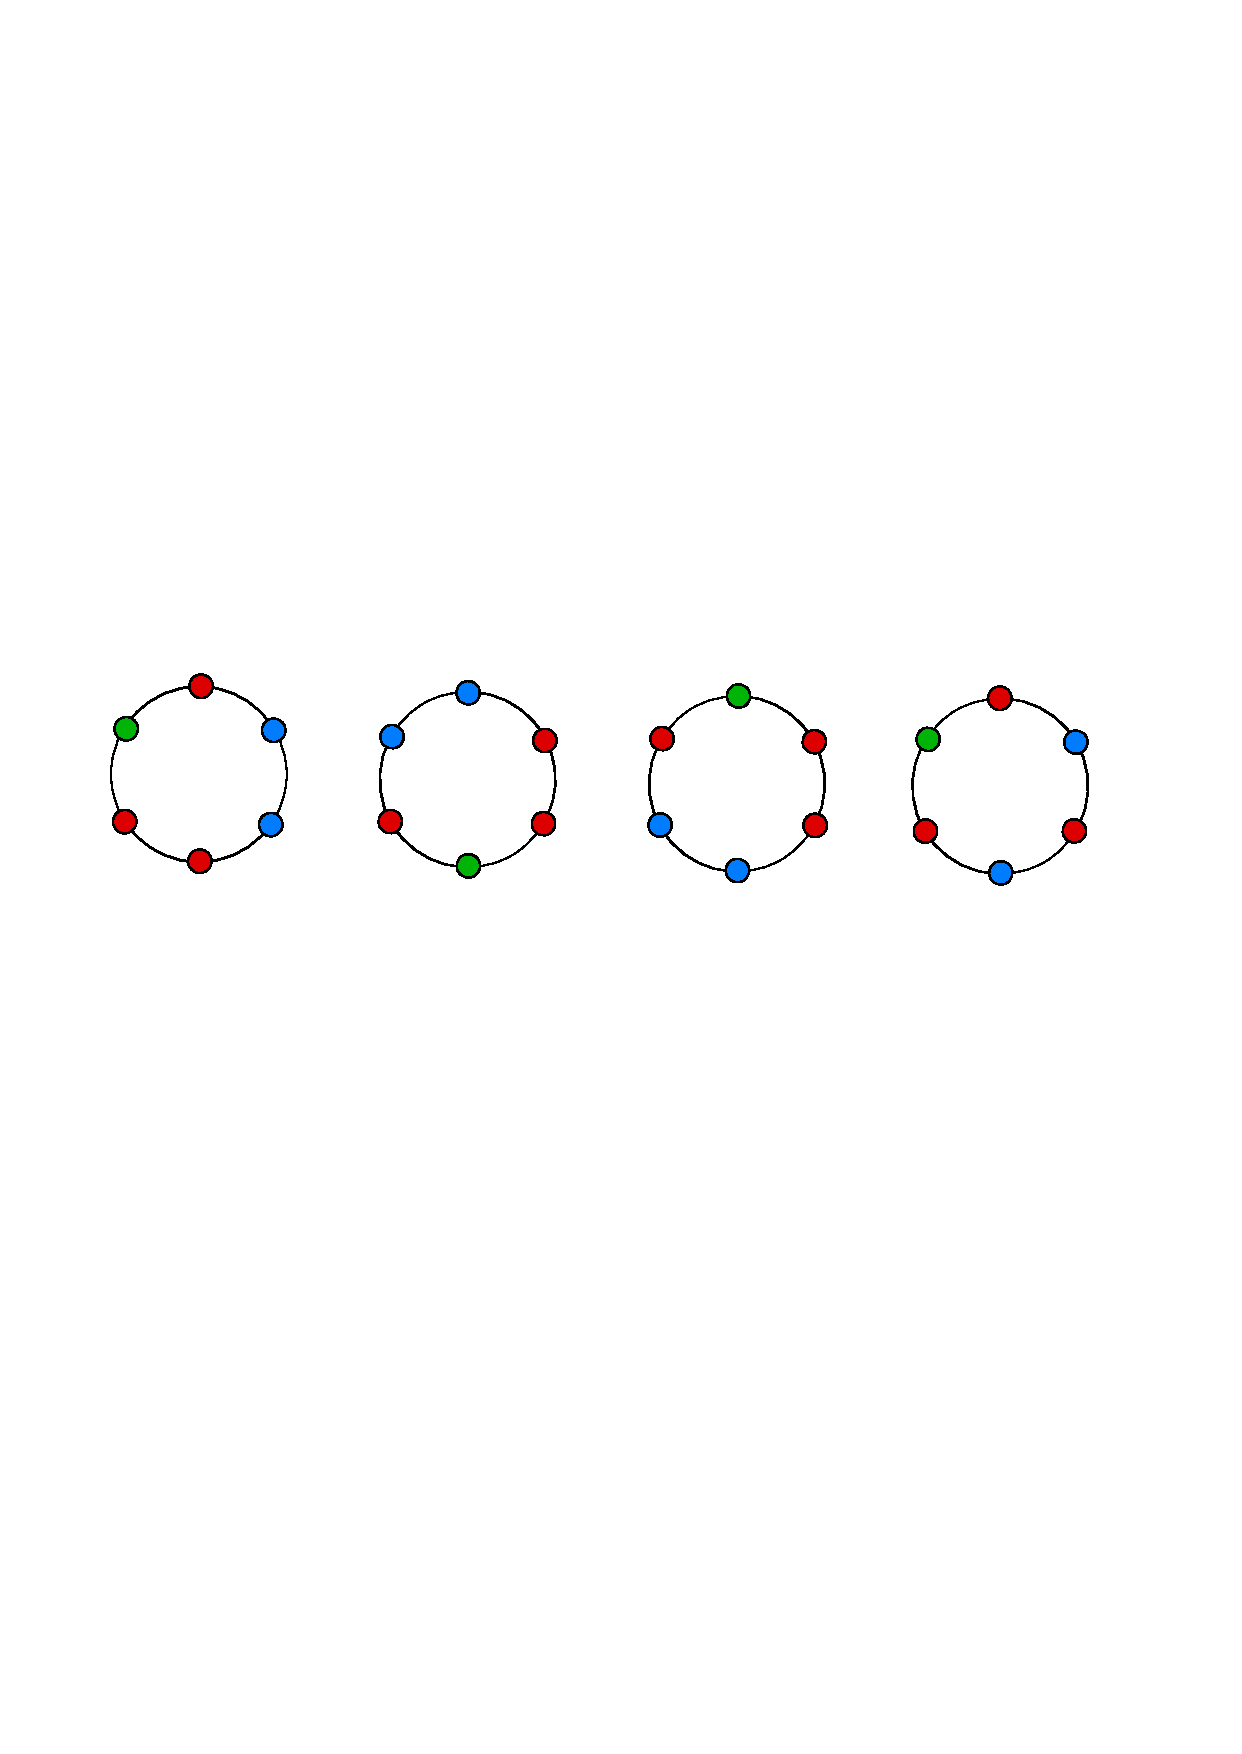
\includegraphics[viewport=44 401 537 528, scale=.6]{intro-figs/necklaces}\\
\caption{Necklaces made with three colors} 
\label{fig:intro:necklace}
\end{center}
\end{figure}


\begin{enumerate}
\item How many different necklaces of six beads can be formed using three reds, two
blues and one green?
\item How many different necklaces of six beads can be formed using red, blue and green
beads (not all colors have to be used)?
\item How many different necklaces of six beads can be formed using red, blue and green
beads if all three colors have to be used?
\item How would we possibly answer these questions for necklaces of six 
thousand beads made with beads from three thousand different colors?
What special software would be required to find the exact answer and how
long would the computation take?
\end{enumerate}

\section{Combinatorics and Graph Theory}\label{s:intro:graph}

A \textit{graph} $G$ consists of a \textit{vertex} set $V$ and
a collection $E$ of $2$-element subsets of $ V$. Elements of $E$ are
called edges.  In our course, we will (almost always) use the convention
that $V=\{1,2,3,\dots,n\}$ for some positive integer~$n$.  With
this convention, graphs can be described \textit{precisely}
with a text file:
\begin{enumerate}
\item The first line of the file contains a single integer $n$, the
number of vertices in the graph.
\item Each of the remaining lines of the file contains a pair of 
distinct integers and specifies an edge of the graph.
\end{enumerate}
We illustrate this convention in \autoref{fig:graphdata} with a text 
file and the diagram for the graph~$G$ it defines.

\hspace{.5in}
\begin{figure}
\begin{minipage}{1.5in}
\texttt{graph1.txt}\\
9\\
6 2\\
1 5\\
1 7\\
6 8\\
9 1\\
4 3\\
5 7\\
1 3\\
5 9\\
7 9
\end{minipage}
\begin{minipage}{3in}
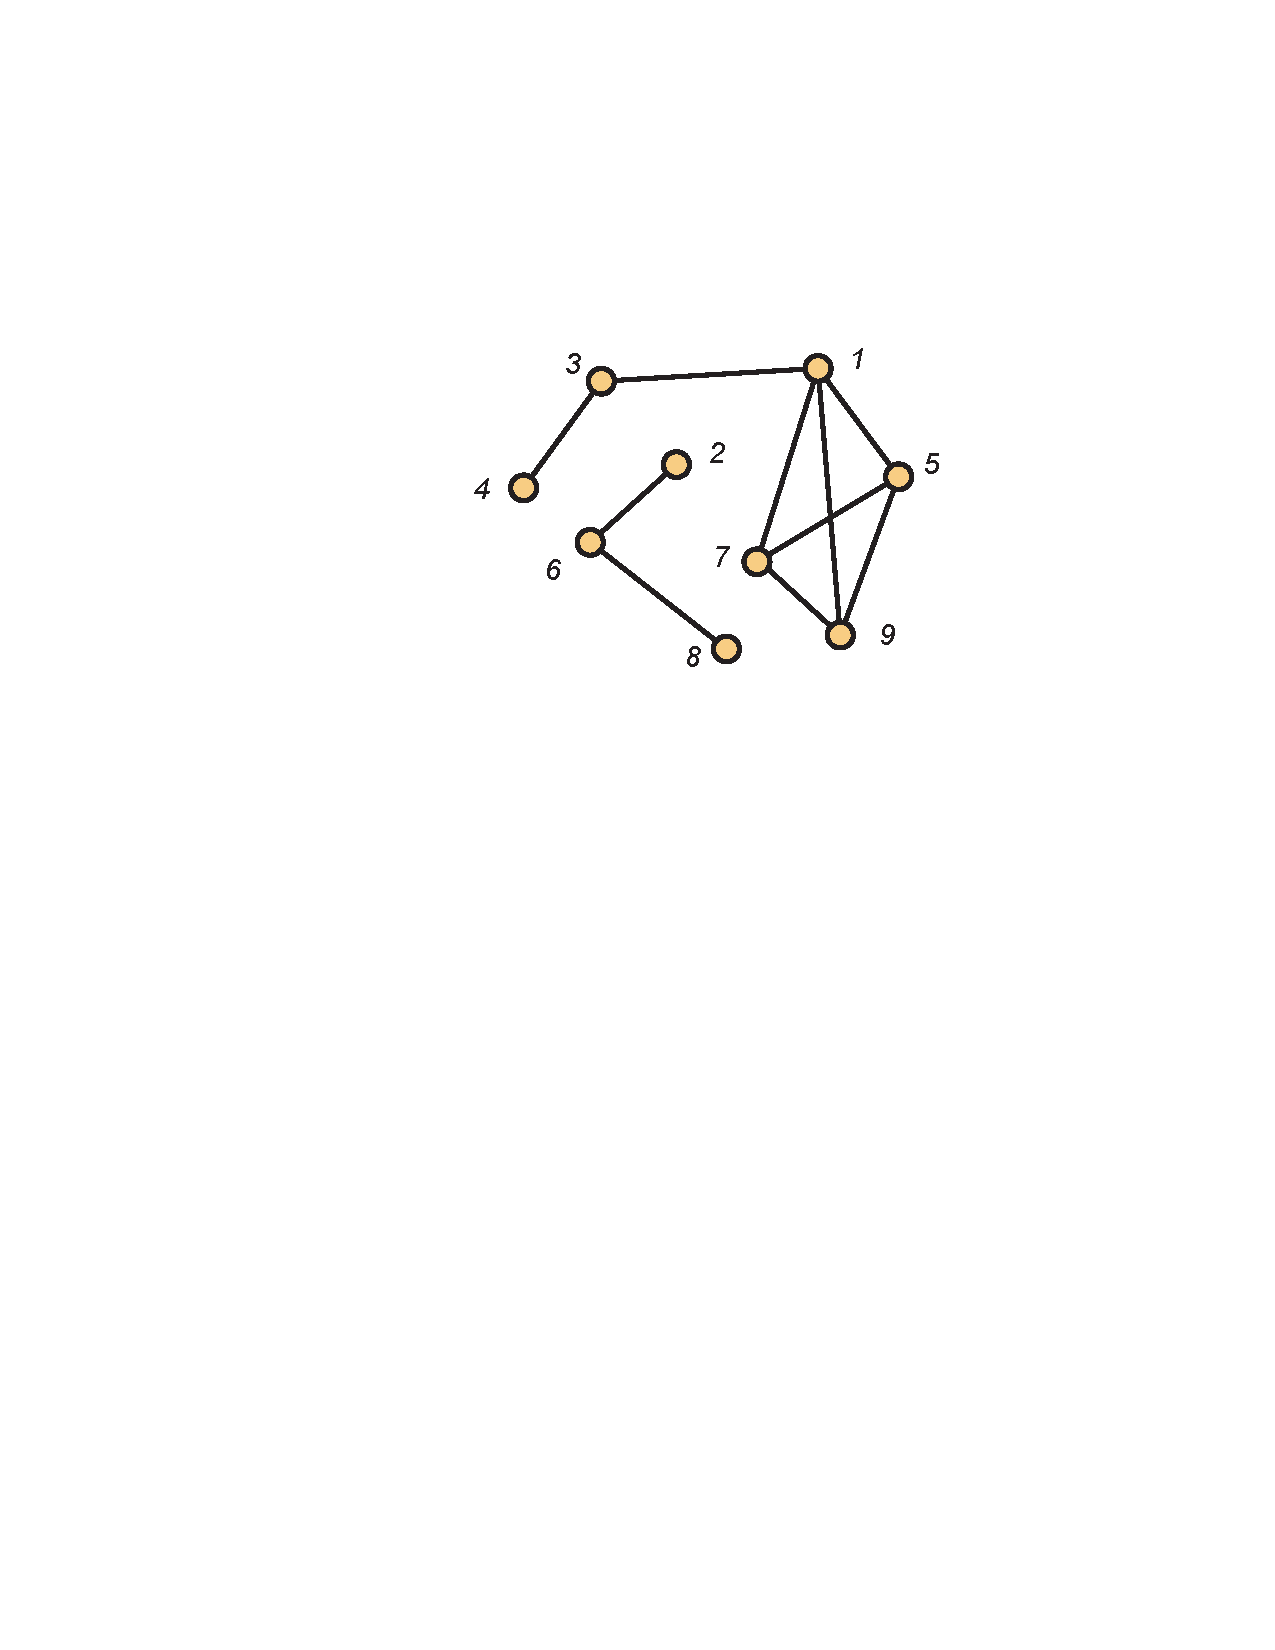
\includegraphics[viewport=223 457 460 629, scale=.6]{intro-figs/3012-fig15}\\
\caption{A graph defined by data}
\label{fig:graphdata}
\end{minipage}
\end{figure}

\medskip
Much of the notation and terminology for graphs is quite natural.
See if you can make sense out of the following statements which
apply to the graph $G$ defined above:
\begin{enumerate}
\item $G$ has $9$ vertices and $10$ edges.
\item $\{2,6\}$ is an edge.
\item Vertices $5$ and $9$ are adjacent.
\item $\{5,4\}$ is not an edge.
\item Vertices $3$ and $7$ are not adjacent.
\item $P = (4, 3,1, 7,9,5)$ is a path 
of length~$5$ from vertex $4$ to vertex~$5$.
\item $C=(5,9,7,1)$ is cycle of length~$4$.
\item $G$ is disconnected and has two components.
One of the components has vertex set $\{2,6,8\}$.
\item $\{1,5,7\}$ is a triangle.
\item $\{1,7,5,9\}$ is a clique of size~$4$.
\item $\{4,2,8,5\}$ is an independent set of
size~$4$.
\end{enumerate}

Equipped only with this little bit of background
material, we are already able to pose a number
of interesting and challenging problems.  

\begin{example}
Consider the graph $G$ shown in \autoref{fig:connectedgraph}.

\begin{figure}
\begin{center}
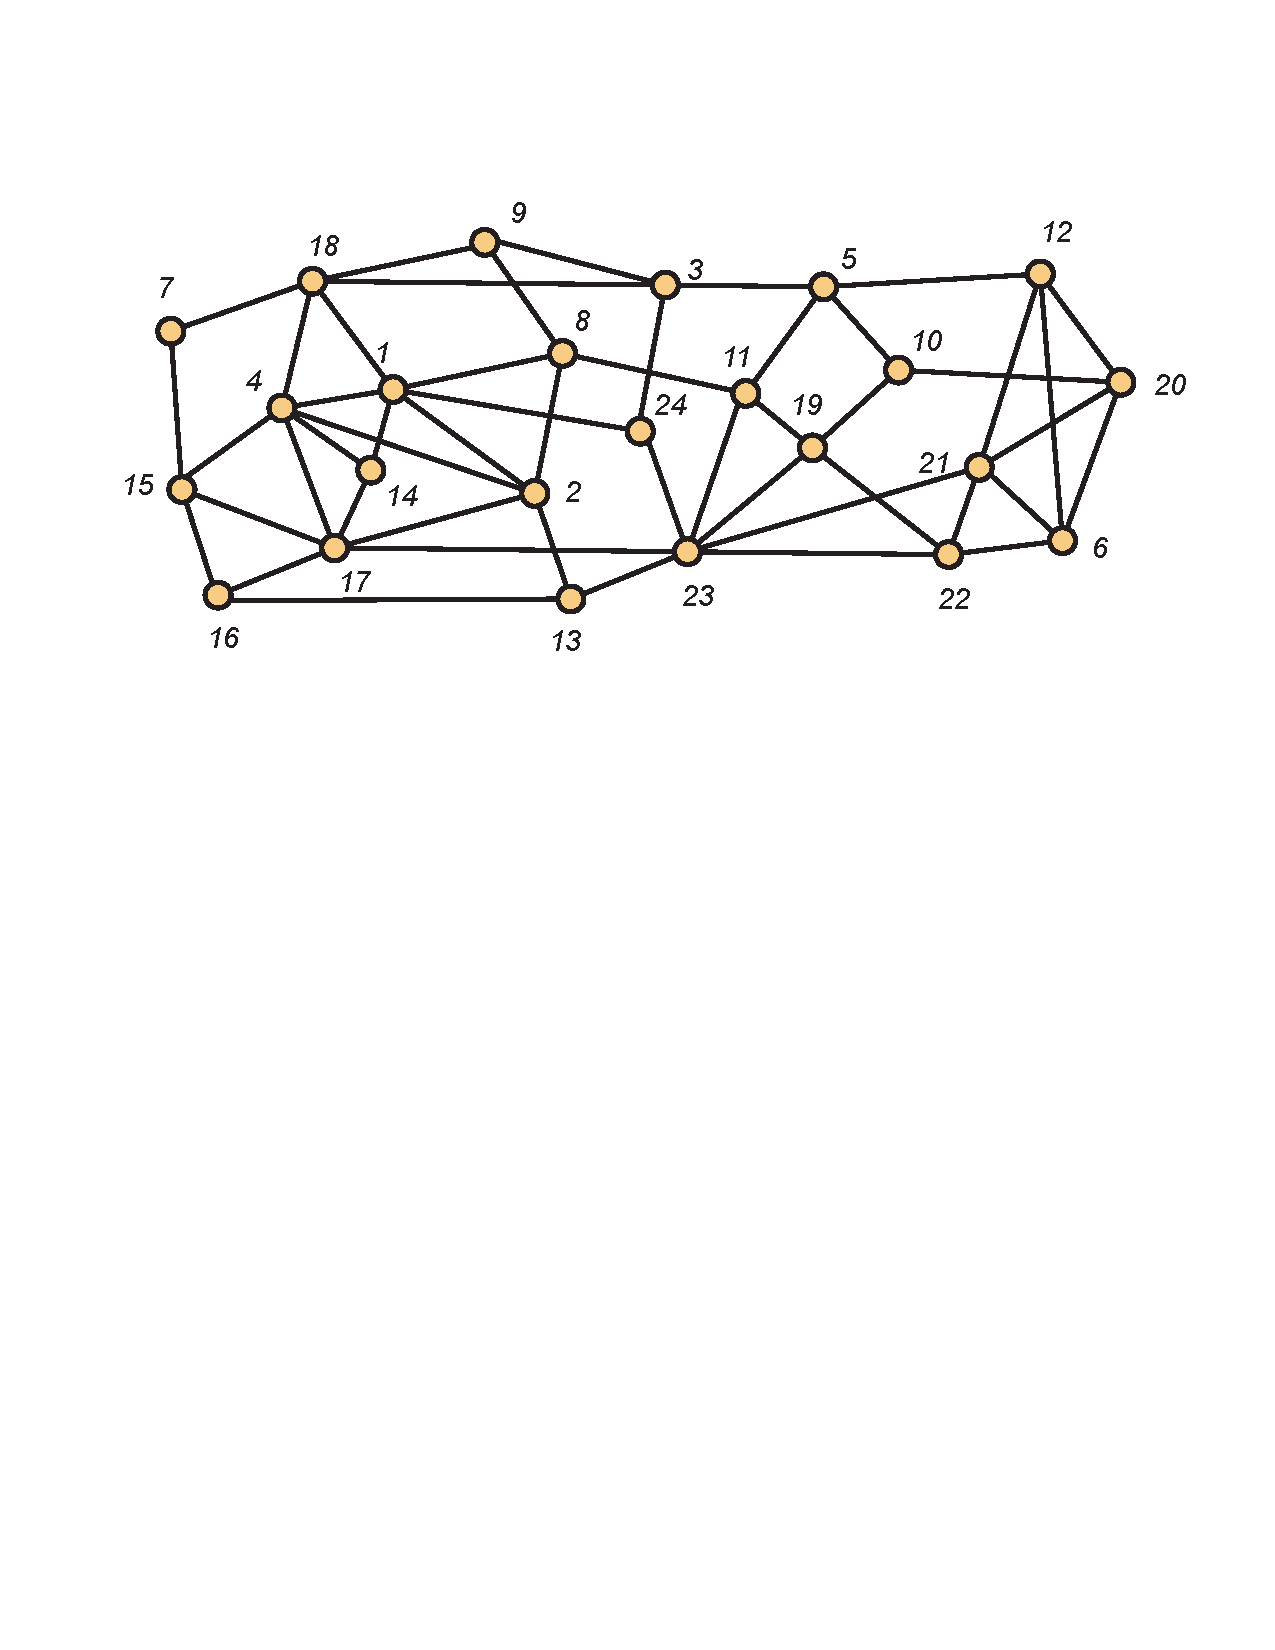
\includegraphics[viewport=55 462 575 702, scale=.6]{intro-figs/3012-fig17}\\
\caption{A connected graph}
\label{fig:connectedgraph}
\end{center}
\end{figure}

\begin{enumerate}
\item What is the largest $k$ for which $G$ has a path
of length~$k$? 
\item What is the largest $k$ for which $G$ has a cycle 
of length~$k$? 
\item What is the largest $k$ for which $G$ has a clique
of size~$k$? 
\item What is the largest $k$ for which $G$ has an
independent set of size~$k$? 
\item  What is the shortest path from vertex~$7$ to
vertex~$6$?
\end{enumerate}

Suppose we gave the class a text data file for a graph
on $1500$ vertices and asked whether the graph contains
a cycle of length at least $500$.  Raoul says yes and
Carla says no. How do we decide who is right?

Suppose instead we asked whether the graph has a clique of
size~$500$.  Helene says that she doesn't think so, but isn't
certain.  Is it reasonable that her classmates insist that
she make up her mind, one way or the other?  Is determining whether
this graph has a clique of size~$500$ harder, easier or
more or less the same as determining whether
it has a cycle of size~$500$.
\end{example}

We will frequently study problems in which graphs
arise in a very natural manner.  Here's an example.

\begin{example}\label{ex:radiostations}
In \autoref{fig:radiostations}, we show the location of some radio stations in the
plane, together with a scale indicating a distance of~$200$ miles.
Radio stations that are closer than~$200$ miles apart must broadcast
on different frequencies to avoid interference.  

\begin{figure}
\begin{center}
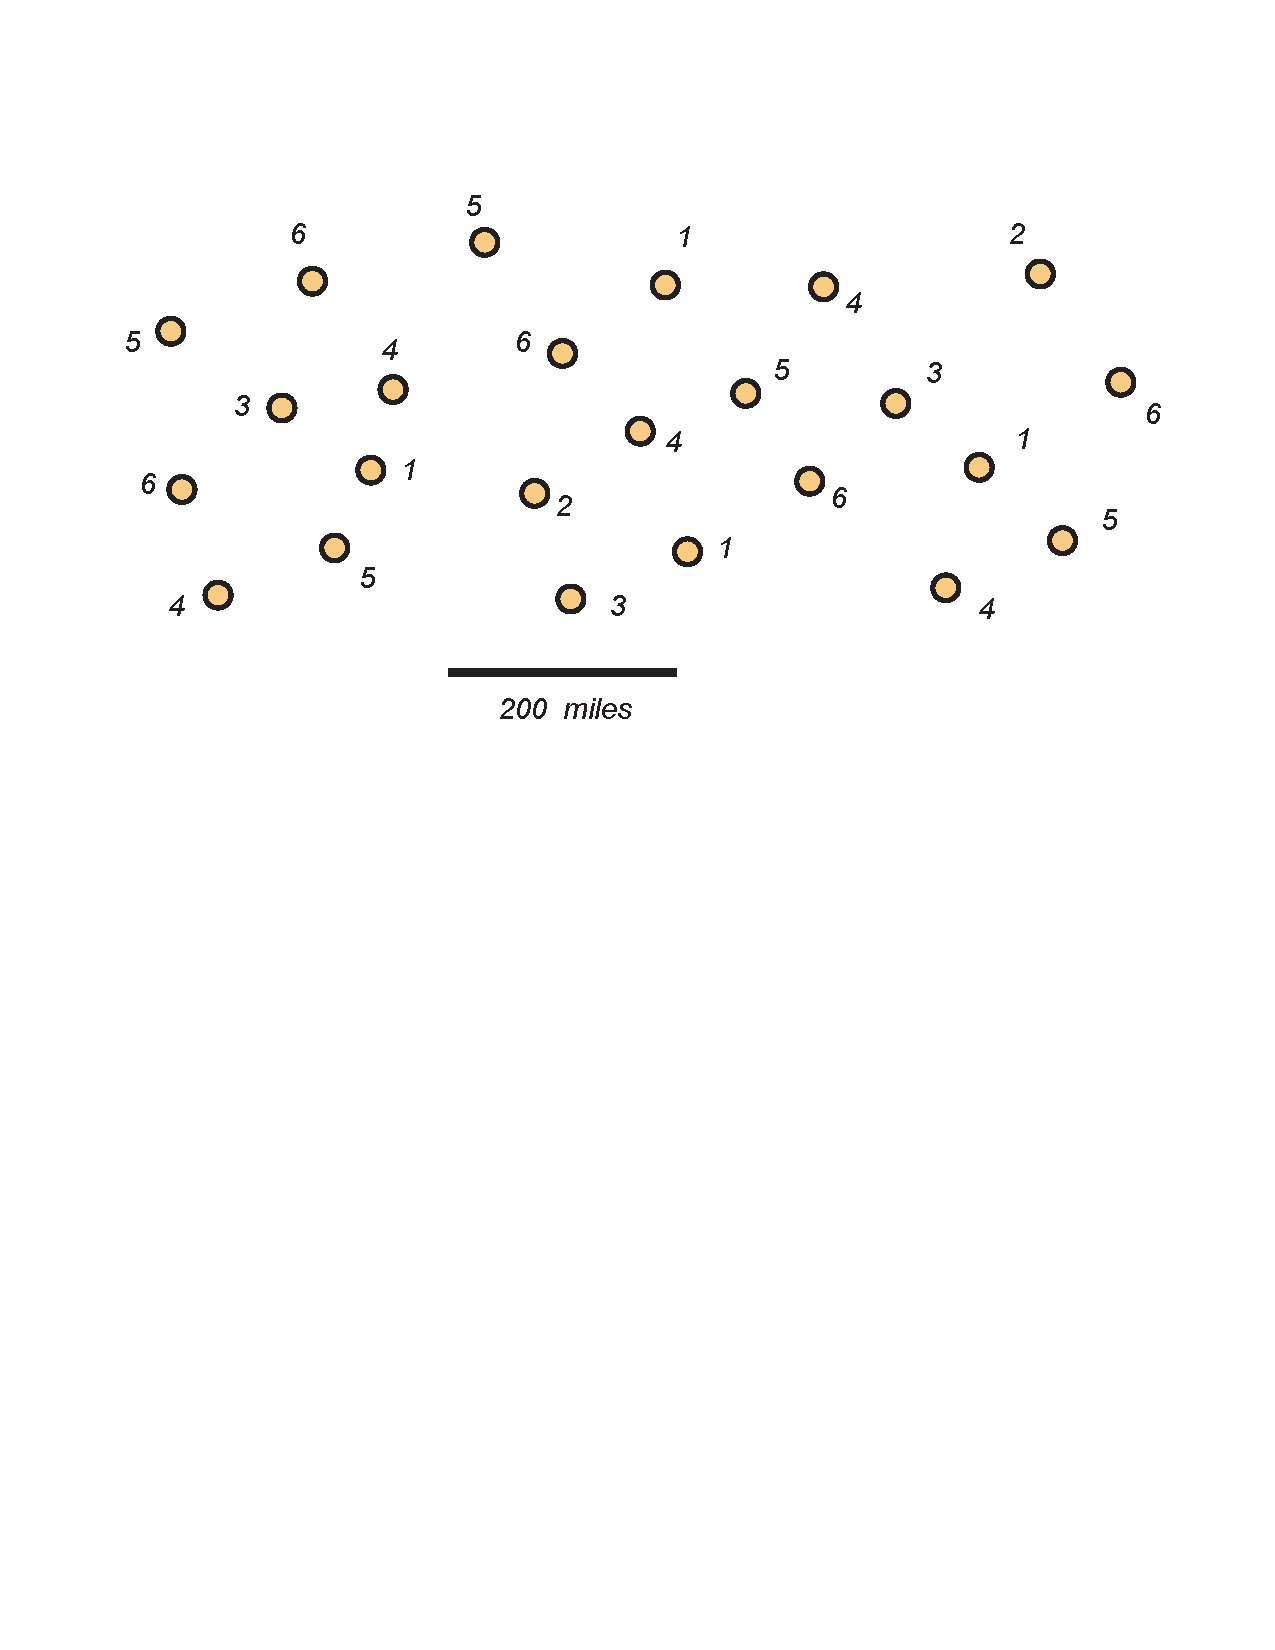
\includegraphics[viewport=46 433 576 706, scale=.6]{intro-figs/3012-fig4}\\
\end{center}
\caption{Radio Stations}
\label{fig:radiostations}
\end{figure}

We've shown that~$6$ different frequencies are enough.  
Can you do better?

Can you find~$4$ stations each of which is within
$200$ miles of the other~$3$?  Can you find $8$ stations each of is more
than $200$ miles away from the other~$7$?   Is there a natural
way to define a graph associated with this problem?
\end{example}

\begin{example}
How big must an applied combinatorics class be so that there are
either (a)~six students with each pair having taken at least one
other class together, or (b)~six students with each pair together
in a class for the first time.  Is this really a hard problem or
can we figure it out in just a few minutes, scribbling on a napkin?
\end{example}
 
\section{Combinatorics and Number Theory}\label{s:intro:number}

Broadly, number theory concerns itself with the properties of the
positive integers. G.H.\ Hardy was a brilliant British mathematician
who lived through both World Wars and conducted a large deal of
number-theoretic research. He was also a pacifist who was happy that,
from his perspective, his research was not ``useful''. He wrote in his
1940 essay \emph{A Mathematician's Apology} ``[n]o one has yet
discovered any warlike purpose to be served by the theory of numbers
or relativity, and it seems very unlikely that anyone will do so for
many years.''\footnote{G.H.\ Hardy, \textit{A Mathematician's
    Apology}, Cambridge University Press, p. 140. (1993 printing)}
Little did he know, the purest mathematical ideas of number theory
would soon become indispensable for the cryptographic techniques that
kept communications secure. Our subject here is not number theory, but
we will see a few times where combinatorial techniques are of use in
number theory.

\begin{example}\label{ex:collatz}
Form a sequence of positive integers using the
following rules.  Start with a positive integer $n>1$. If $n$ is odd,
then the next number is $3n+1$.  If $n$ is even, then the
next number is $n/2$.  Halt if you ever reach~$1$.
For example, if we start with $28$, the sequence is
\[
28, 14, 7, 22, 11, 34, 17, 52, 26, 13, 40, 20, 10, 5, 16, 8, 4, 2, 1.
\]

Now suppose you start with $19$.  Then the first few terms are
\[
19, 58, 29, 88, 44, 22.
\]
But now we note that the integer $22$ appears in the first sequence,
so the two sequences will agree from this point on.  Sequences formed
by this rule are called \textit{Collatz sequences}.

Pick a number somewhere between $100$ and $200$ and write down the sequence
you get.  Regardless of your choice, you will eventually halt with a~$1$.
However, is there some positive integer $n$ (possibly quite large) so
that if you start from $n$, you will never reach~$1$?
\end{example}
 
\begin{example}
Students in middle school are taught to add fractions by finding
least common multiples.  For example, the least common multiple
of $15$ and $12$ is $60$, so:

\[
\frac{2}{15}+ \frac{7}{12} = \frac{8}{60}+\frac{35}{60} = \frac{43}{60}.
\]

How hard is it to find the least common multiple of two integers?
It's really easy if you can factor them into primes.  For example,
consider the problem of finding the least common multiple
of $351785000$ and  $316752027900$ if you just happen to know that

\begin{align*}
 351785000 = & 2^3\times 5^4\times 7\times19\times 23^2\quad\text{and}\\ 
 316752027900 = & 2^2\times3\times 5^2\times 7^3\times 11\times 23^4. 
\end{align*}
Then the least common multiple is
\begin{align*}
300914426505000 = & 2^3\times3\times 5^4\times 7^3\times 11\times 19\times 23^4.
\end{align*}
So to find the least common multiple of two numbers, we just have
to factor them into primes.  That doesn't sound too hard. For starters, can you
factor $1961$?  OK, how about $1348433$?  Now for a real challenge.
Suppose you are told that the integer
\[
c = 5220070641387698449504000148751379227274095462521
\]
is the product of two primes $a$ and $b$.  Can you find them?

What if factoring is hard?  Can you find the least common multiple of
two relatively large integers, say each with about~$500$ digits, by
another method? How should middle school students be taught to add
fractions?

As an aside, we note that most calculators can't add or multiply two
$20$ digits numbers, much less two numbers with more than~$500$
digits.  But it is relatively straightforward to write a computer
program that will do the job for us.  Also, there are some powerful
mathematical software tools available.  Two very well known examples
are \emph{Maple}\textsuperscript{\tiny\textregistered} and
\emph{Mathematica}\textsuperscript{\tiny\textregistered}.  For example, if you open up a
\emph{Maple} workspace and enter the command:

\begin{center}
\texttt{ifactor(300914426505000)};
\end{center}
then about as fast as you hit the carriage return, you
will get the prime factorization shown above.

Now here's how we made up the challenge problem.  First, we found a
site on the web that lists large primes and found these two values:

\begin{align*}
a = & 45095080578985454453\quad\text{and}\\ 
b = & 115756986668303657898962467957.
\end{align*}
We then used \emph{Maple} to multiply them together using the following command:

\[
45095080578985454453*115756986668303657898962467957;
\]
Almost instantly, \emph{Maple} reported the value for $c$ given above.

Out of curiosity, we then asked \emph{Maple} to factor~$c$.  It took almost
$12$ minutes on a powerful desktop computer.
\end{example}

Questions arising in number theory can also have an enumerative flair,
as the following example shows.

\begin{example}
In \autoref{fig:intro:partsof8}, we show the integer partitions
of~$8$.
\begin{figure}[hb]
%\centering
\begin{multicols}{3}
  8\quad\text{distinct}\\
  7+1\quad\text{distinct and odd}\\
  6+2\quad\text{distinct}\\
  6+1+1\\
  5+3\quad\text{distinct and odd}\\
  5+2+1\quad\text{distinct}\\
  5+1+1+1\quad\text{odd}\\
  4+4\\
  4+3+1\quad\text{distinct}\\
  4+2+2\\
  4+2+1+1\\
  4+1+1+1+1\\
  3+3+2\\
  3+3+1+1\quad\text{odd}\\
  3+2+2+1\\
  3+2+1+1+1\\
  3+1+1+1+1+1\quad\text{odd}\\
  2+2+2+2\\
  2+2+2+1+1\\
  2+2+1+1+1+1\\
  2+1+1+1+1+1+1\\
  1+1+1+1+1+1+1+1\quad\text{odd}  
\end{multicols}
% \begin{tabular}{lll}
%   8\quad\text{distinct parts}&
%   7+1\quad\text{distinct parts, odd parts}&
%   6+2\quad\text{distinct parts}\\
%   6+1+1&
%   5+3\quad\text{distinct parts, odd parts}&
%   5+2+1\quad\text{distinct parts}\\
%   5+1+1+1\quad\text{odd parts}&
%   4+4&
%   4+3+1\quad\text{distinct parts}\\
%   4+2+2&
%   4+2+1+1&
%   4+1+1+1+1\\
%   3+3+2&
%   3+3+1+1\quad\text{odd parts}&
%   3+2+2+1\\
%   3+2+1+1+1&
%   3+1+1+1+1+1\quad\text{odd parts}&
%   2+2+2+2\\
%   2+2+2+1+1&
%   2+2+1+1+1+1&
%   2+1+1+1+1+1+1\\&
%   1+1+1+1+1+1+1+1\quad\text{odd parts}
% \end{tabular}
\caption{The partitions of $8$, noting those into distinct parts
  and those into odd parts.}
\label{fig:intro:partsof8}
\end{figure}
There are~$22$ partitions altogether, and as noted, exactly~$6$
of them are partitions of~$8$ into odd parts.  Also, exactly~$6$ of them
are partitions of~$8$ into distinct parts.

What would be your reaction if we asked you to find the number of
integer partitions of $25892$?  Do you think that the number of
partitions of $25892$ into odd parts equals the number of partitions
of $25892$ into distinct parts?  Is there a way to answer this
question \textit{without} actually calculating the number of
partitions of each type?
\end{example}

\section{Combinatorics and Geometry}\label{s:intro:geom}

There are many problems in geometry that are innately combinatorial or
for which combinatorial techniques shed light on the problem.

\begin{example}  
  In \autoref{fig:linesregions}, we show a family of $4$ lines in
  the plane.  Each pair of lines intersects and no point in the plane
  belongs to more than two lines.  These lines determine~$11$ regions.

\begin{figure}[hbt]
\begin{center}
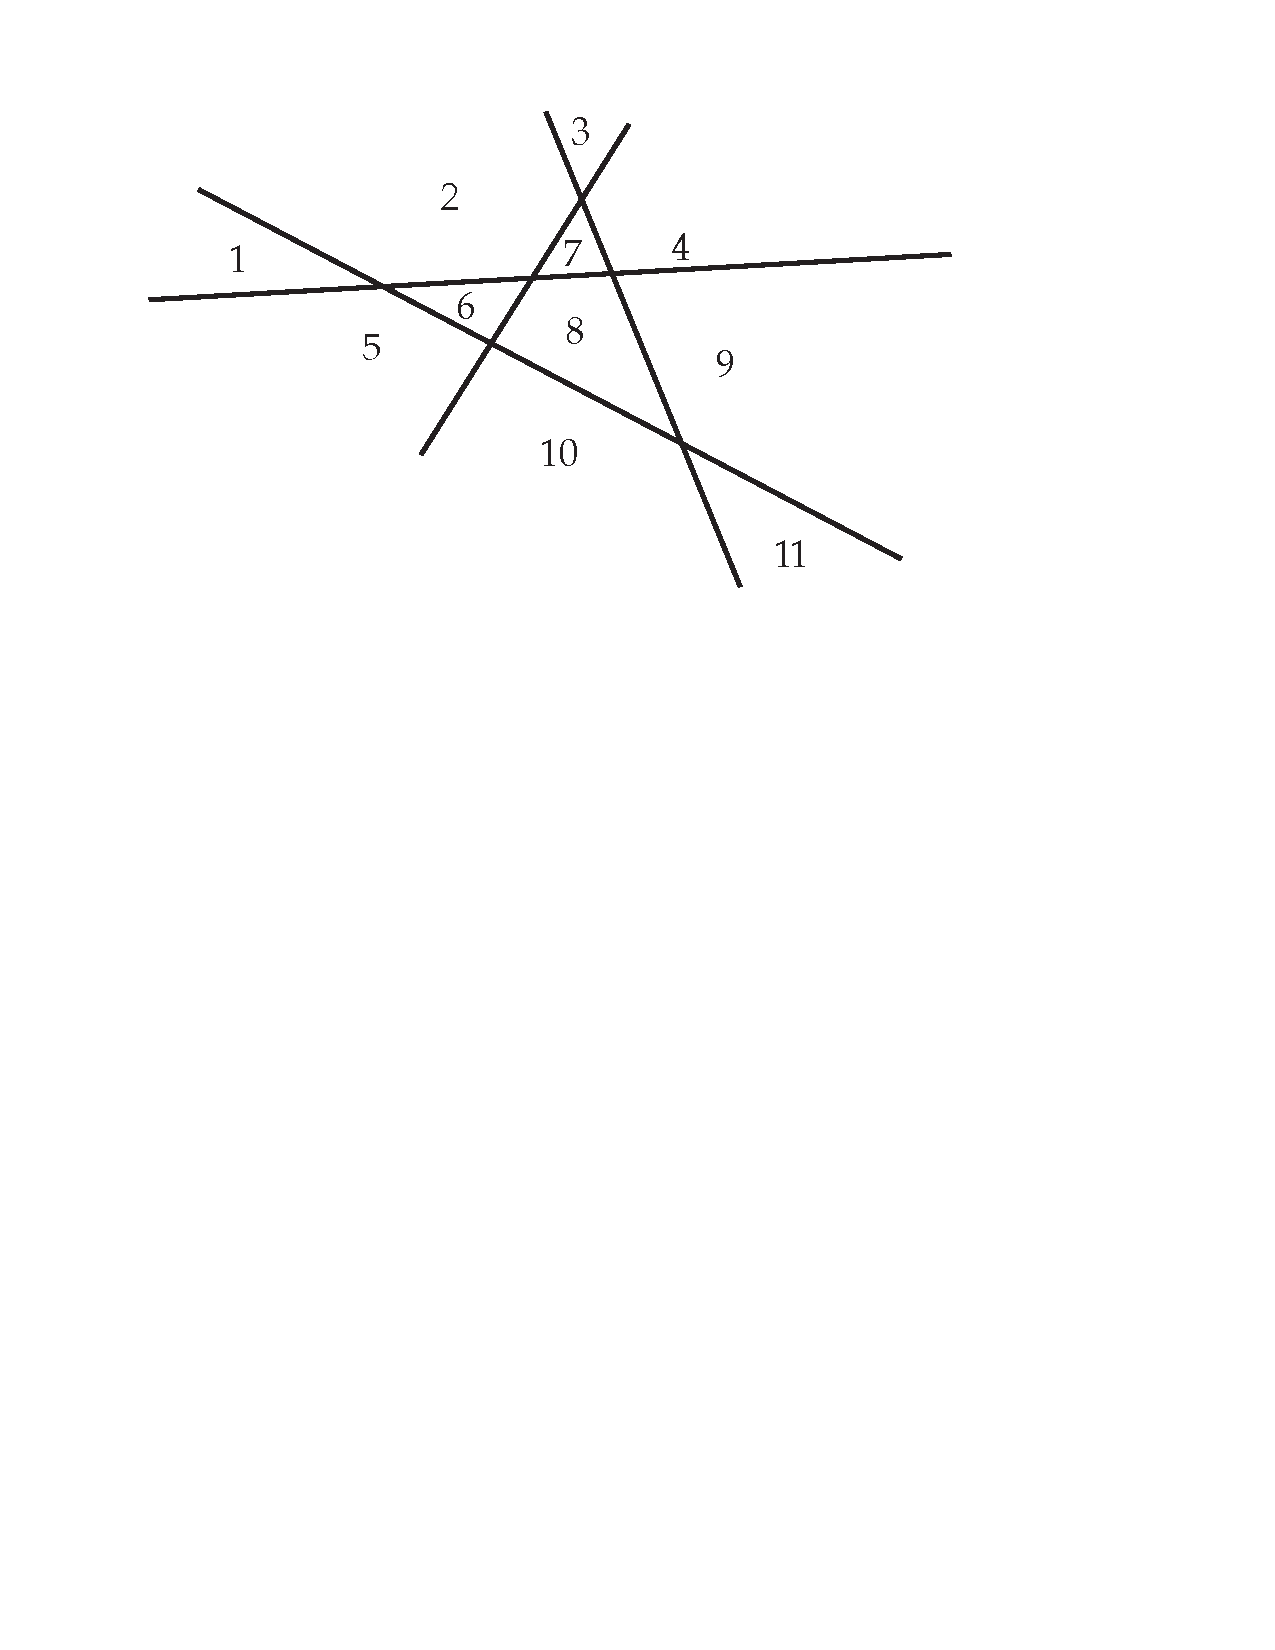
\includegraphics[viewport=60 480 470 745, scale=.6]{intro-figs/3012-fig9}\\
\end{center}
\caption{Lines and regions}
\label{fig:linesregions}
\end{figure}

Under these same restrictions, how many regions would a family of
$8947$ lines determine?  Can different arrangements of lines determine
different numbers of regions?
\end{example}

\begin{example}
Mandy says she has found a set of~$882$ points in the plane that
determine exactly $752$ lines.  Tobias disputes her claim.
Who is right?
\end{example}

\begin{example}
There are many different ways to draw a graph in the plane. Some
drawings may have crossing edges while others don't.  But sometimes, crossing
edges must appear in any drawing.
Consider the graph $G$ shown in \autoref{fig:crossingedges}.
\begin{figure}
\begin{center}
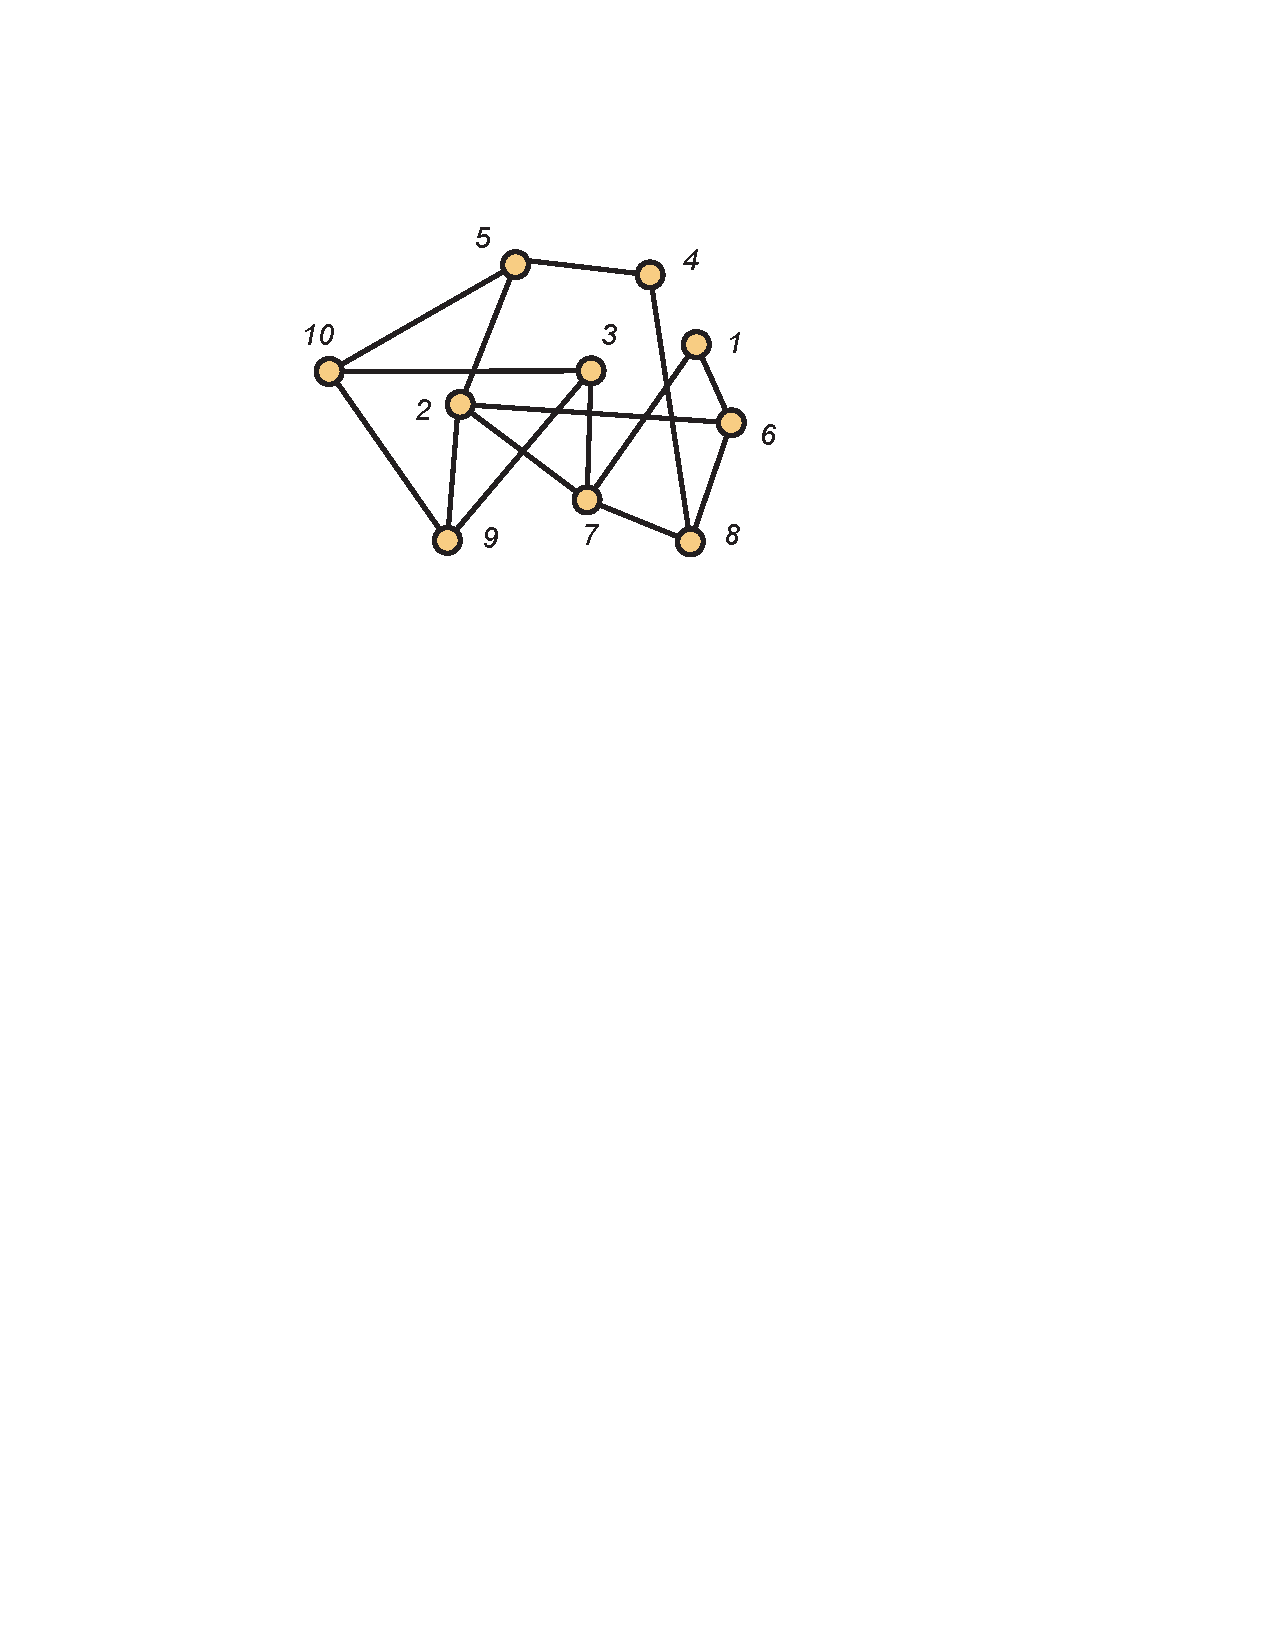
\includegraphics[viewport=132 509 372 683, scale=.6]{intro-figs/3012-fig8}\\
\end{center}
\caption{A graph with crossing edges}
\label{fig:crossingedges}
\end{figure}
Can you redraw $G$ without crossing edges?

Suppose Sam and Deborah were given a homework problem asking whether a
particular graph on $2843952$ vertices and $9748032$ edges could be
drawn without edge crossings.  Deborah just looked at the number of
vertices and the number of edges and said that the answer is ``no.''
Sam questions how she can be so certain---without looking more
closely at the structure of the graph.  Is there a way for
Deborah to justify her definitive response?
\end{example}

\section{Combinatorics and Optimization}\label{s:intro:opt}

You likely have already been introduced to optimization problems, as
calculus students around the world are familiar with the plight of
farmers trying to fence the largest area of land given a certain
amount of fence or people needing to cross rivers downstream from
their current location who must decide where they should cross based
on the speed at which they can run and swim. However, these problems
are inherently continuous. In theory, you can cross the river at any
point you want, even if it were irrational. (OK, so not exactly
irrational, but a good decimal approximation.) In this course, we will
examine a few optimization problems that are not continuous, as only
integer values for the variables will make sense. It turns out that
many of these problems are very hard to solve in general.

\begin{example}
In \autoref{fig:wgraph-1}, we use letters for the labels on the
vertices to help distinguish visually from the integer weights
on the edges. 

\begin{figure}
\begin{center}
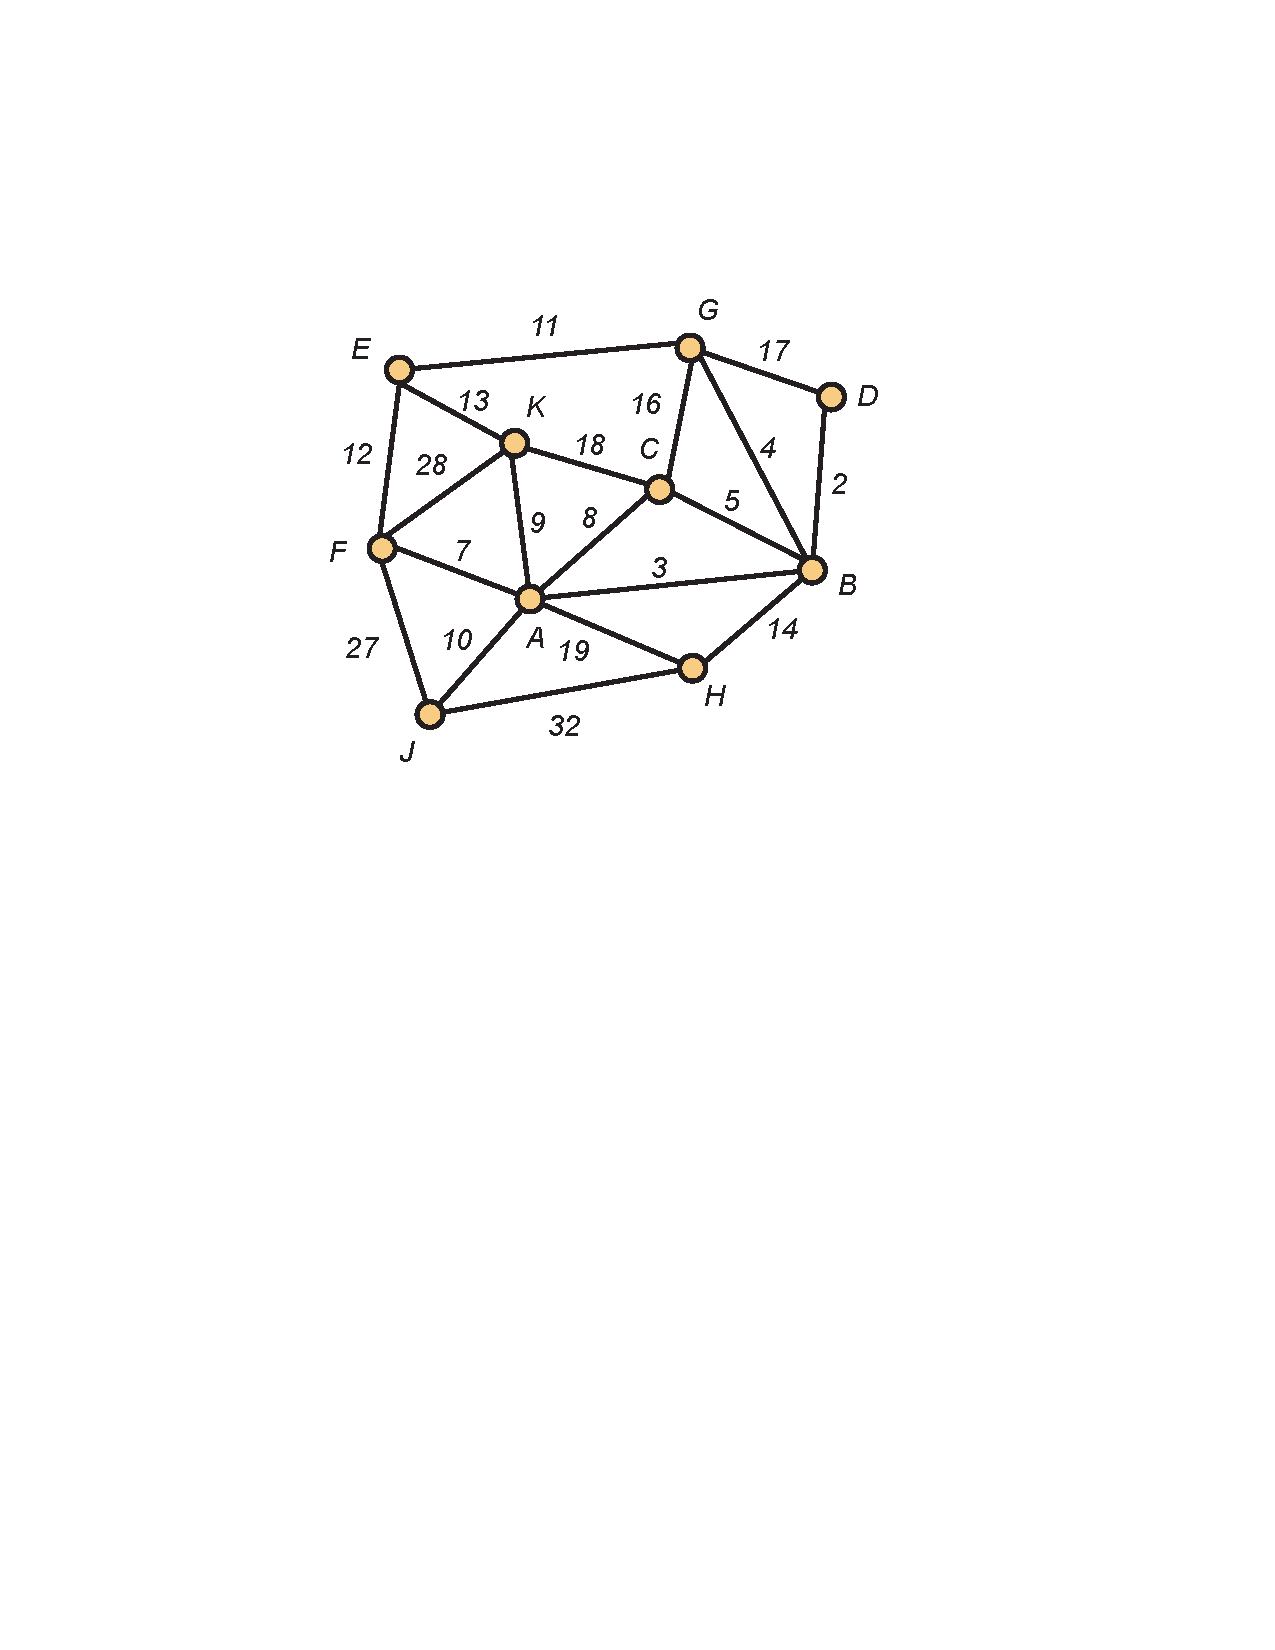
\includegraphics[viewport=140 413 430 650, scale=.6]{intro-figs/3012-fig12}\\
\end{center}
\caption{A labeled graph with weighted edges}
\label{fig:wgraph-1}
\end{figure}

Suppose the vertices are cities, the edges are highways
and the weights on the edges represent \textit{distance}.

\medskip
\noindent
$Q_1$:\quad  What is the shortest path from vertex~$E$ to vertex~$B$?

\medskip
Suppose Ariel is a salesperson whose home base is city~$A$. 

\medskip
\noindent
$Q_2$:\quad In what order should Ariel visit the other cities so that she
goes through each of them at least once and returns home
at the end---while keeping the total distance traveled to a minimum?  
Can Ariel accomplish such a tour visiting
each city \textit{exactly} once? 

\medskip
Sanjay is a highway inspection engineer and must traverse every
highway each month.  Sanjay's homebase is City~$E$.  

\medskip
\noindent
$Q_3$:\quad In what
order should Sanjay traverse the highways to minimize the total
distance traveled?  Can Sanjay make such a tour traveling
along each highway exactly once?
\end{example}

\begin{example}
  Now suppose that the vertices are locations of branch banks in
  Atlanta and that the weights on an edge represents the cost, in
  millions of dollars, of building a high capacity data link between
  the branch banks at it two end points.  In this model, if there is
  no edge between two branch banks, it means that the cost of building
  a data link between this particular pair is prohibitively high (here
  we might be tempted to say the cost is infinite, but the authors don't
  admit to knowing the meaning of this word).

  Our challenge is to decide which data links should be constructed to
  form a network in which any branch bank can communicate with any
  other branch.  We assume that data can flow in either direction on a
  link, should it be built, and that data can be relayed through any
  number of data links.  So to allow full communication, we should
  construct a \textit{spanning tree} in this network.  In
  \autoref{fig:spantree-1}, we show a graph $G$ on the left and one of
  its many \textit{spanning trees} on the right.

\begin{figure}
\begin{center}
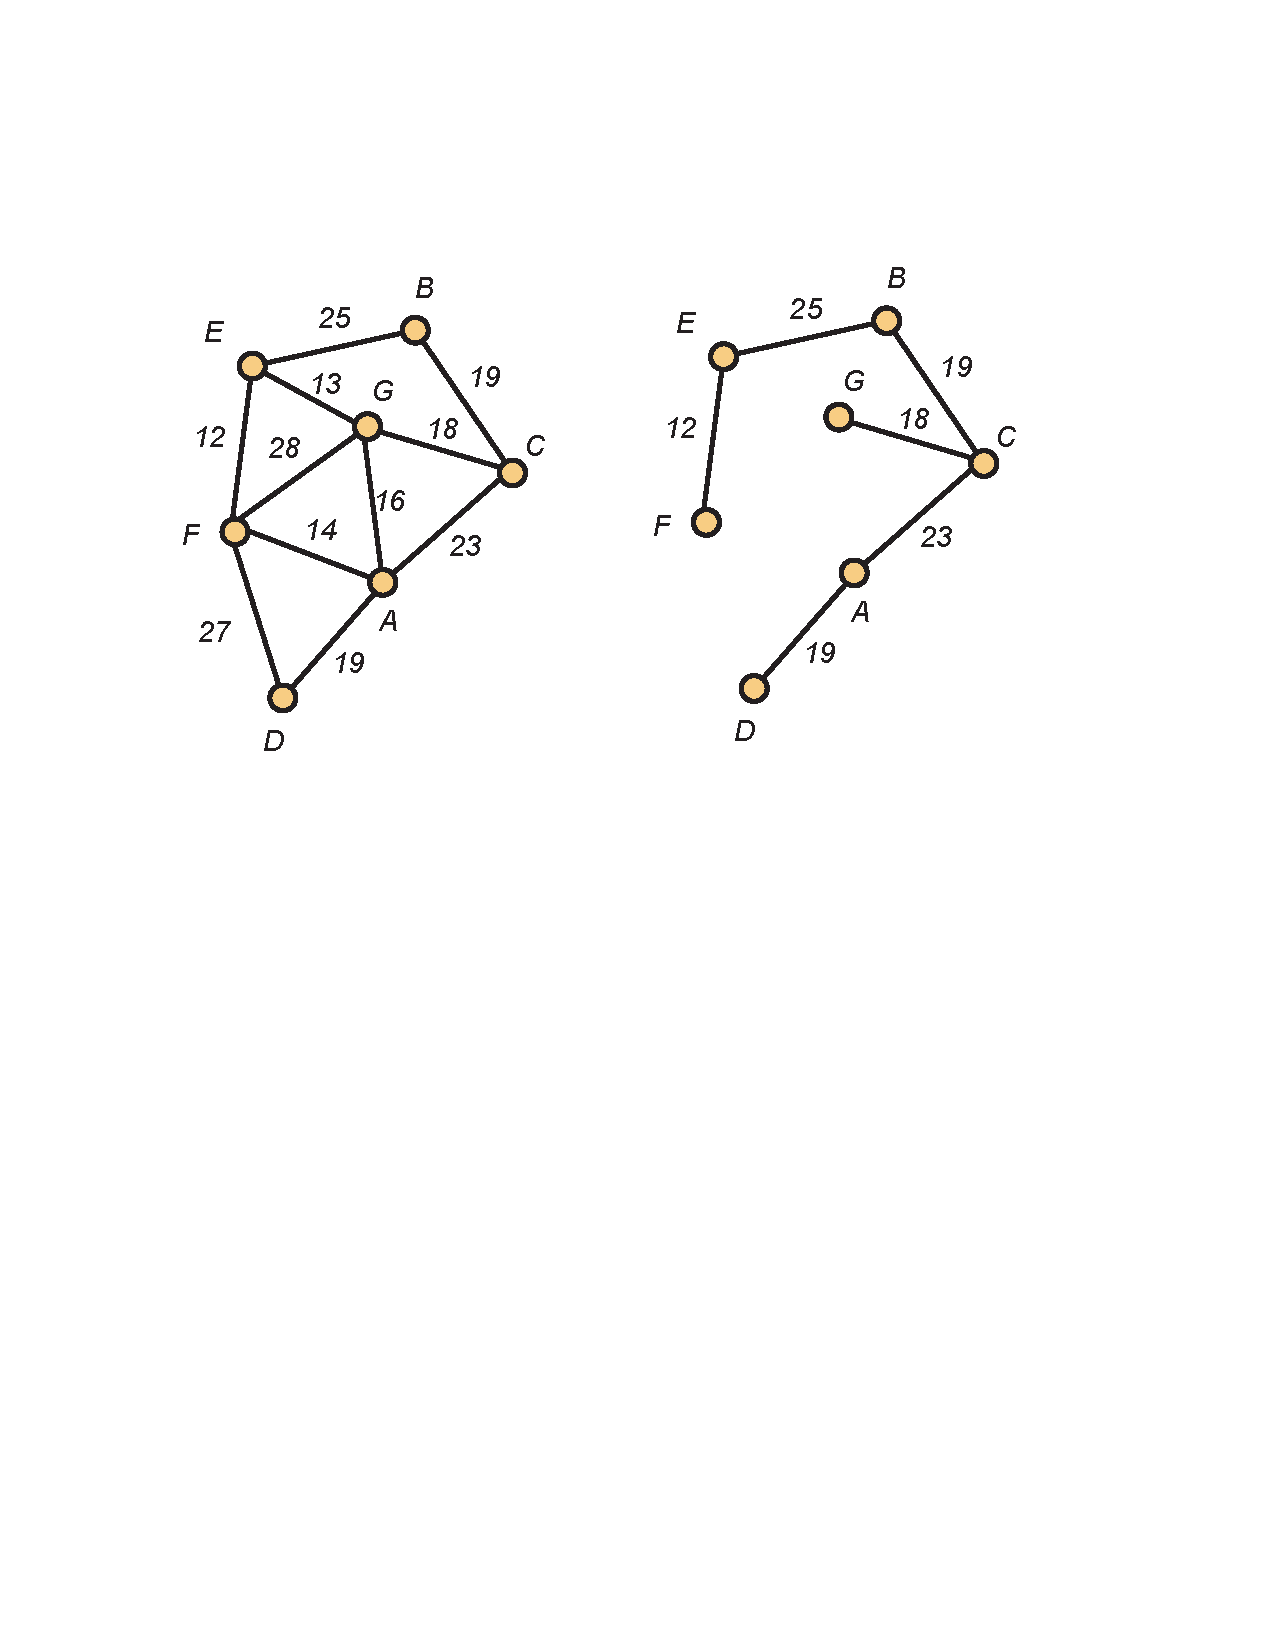
\includegraphics[viewport=82 420 500 677, scale=.6]{intro-figs/3012-fig19}\\
\end{center}
\caption{A weighted graph and spanning tree}
\label{fig:spantree-1}
\end{figure}

The weight of the spanning tree is the sum of the weights on the
edges.  In our model, this represents the costs, again in millions of
dollars, of building the data links associated with the edges in the
spanning tree.  For the spanning tree shown in
\autoref{fig:spantree-1}, this total is
\[
12+25+19+18+23+19 = 116.
\]
Of all spanning trees, the bank would naturally like to find one
having minimum weight.

How many spanning trees does this graph have?  For a large graph, say
one with $2875$ vertices, does it make sense to find all spanning
trees and simply take the one with minimum cost?  In particular, for a
positive integer~$n$, how many trees have vertex set
$\{1,2,3,\dots,n\}$?
\end{example}

\section{Sudoku Puzzles}\label{s:intro:sudoku}

Here's an example which has more substance than you might
think at first glance.  It involves Sudoku puzzles, which
have become immensely popular in recent years.
\begin{example}
  A Sudoku puzzle is a $9\times 9$ array of cells that when completed
  have the integers $1,2,\dots,9$ appearing exactly once in each row
  and each column.  Also (and this is what makes the puzzles so
  fascinating), the numbers $1$, $2$, $3,\dots,9$ appear once in each
  of the nine $3\times 3$ subquares identified by the darkened
  borders.  To be considered a legitimate Sudoku puzzle, there should
  be a \textit{unique} solution.  In \autoref{fig:sudoku}, we show two
  Sudoku puzzles.  The one on the right is fairly easy, and the one on
  the left is far more challenging.

\begin{figure}[hb]
\begin{center}
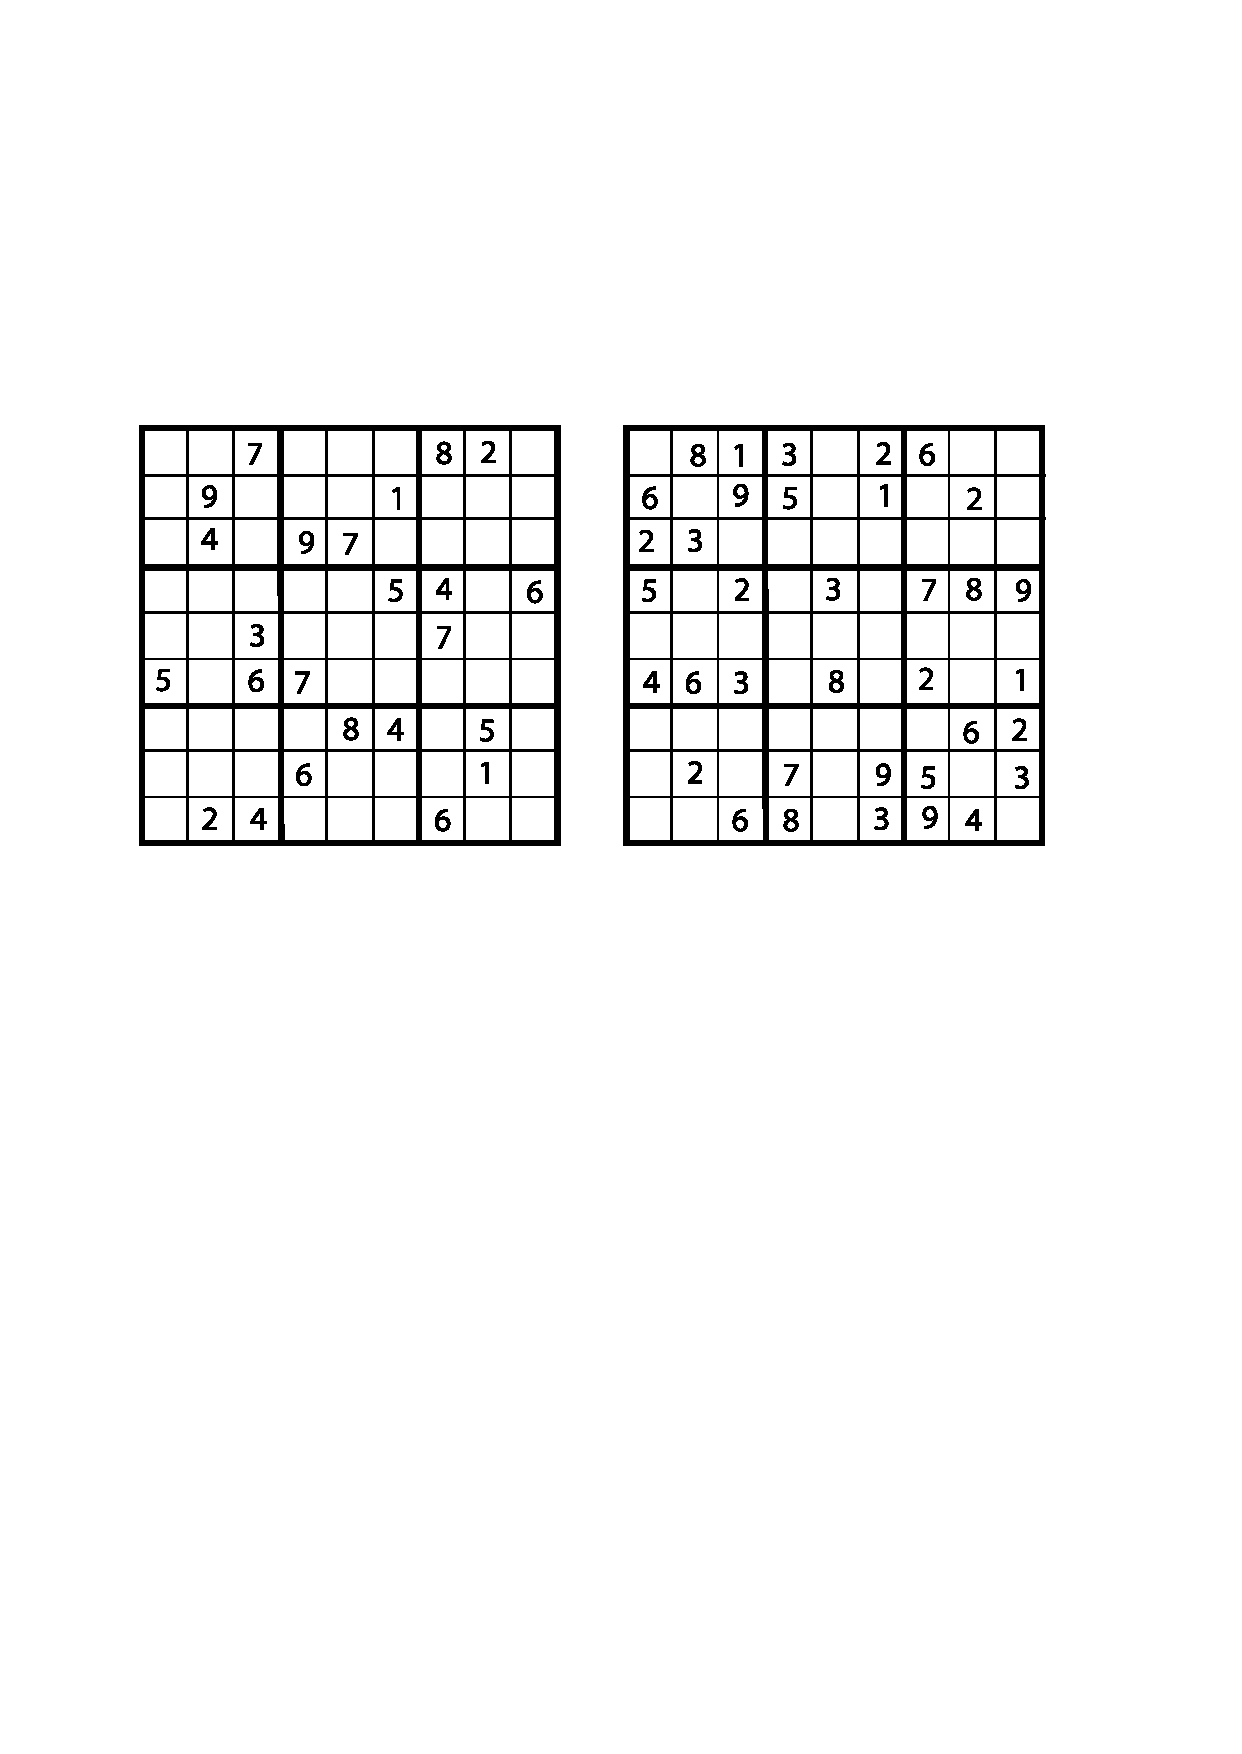
\includegraphics[viewport=60 428 509 645, scale=.8]{intro-figs/mysudoku}\\
\end{center}
\caption{Sudoku puzzles}
\label{fig:sudoku}
\end{figure}

There are many sources of Sudoku puzzles, and software that generates
Sudoku puzzles and then allows you to play them with an attractive GUI
is available for all operating systems we know anything about (although
not recommend to play them during class!).  Also, you can find 
Sudoku puzzles on the web at:

\medskip
\begin{center}
\href{http://www.websudoku.com}.
\end{center}

\medskip
\noindent
On this site, the ``Evil'' ones are just that.

How does Rory make up good Sudoku puzzles, ones that are difficult
for Mandy to solve?  How could Mandy use
a computer to solve puzzles that Rory has constructed? 
What makes some Sudoku puzzles easy and some of them hard?

The size of a Sudoku puzzle can be expanded in an obvious
way, and many newspapers include a $16\times16$ Sudoku puzzle
in their Sunday edition (just next to a challenging crosswords puzzle).
How difficult would it be to solve a $1024\times1024$ Sudoku puzzle,
even if you had access to a powerful computer?
\end{example}

\section{Discussion}\label{s:intro:closing}

Over coffee after their first combinatorics class, Xing remarked
''This doesn't seem to be going like calculus.  I'm expecting
the professor to teach us how to solve problems---at least some
kinds of problems.  Instead, a whole bunch
of problems were posed and we were asked whether 
\textit{we} could solve them.'' Yolanda jumped in ``You may be 
judging things too quickly.  I'm fascinated by these kinds
of questions.  They're different.''  Zori grumpily layed
bare her concerns
``After getting out of Georgia Tech, who's going to pay me to
count necklaces, distribute library books or solve Sudoku puzzles.''
Bob politely countered ``But the problems on networks and graphs
seemed to have practical applications.  I heard my uncle, a very
successful business guy, talk about franchising problems that
sound just like those.''  Alice speculated ``All those network problems
sound the same to me.  A fair to middling computer science major could 
probably write programs to solve any of them.''  Dave mumbled ``Maybe not.
Similar sounding problems might actually be quite different in the end.  
Maybe we'll learn to tell the difference.'' 
After a bit of quiet time interrupted only by latte's disappearing,
Carlos said softly ``It might not be so easy to distinguish hard 
problems from easy ones.'' Alice followed ``Regardless, what strikes 
me is that we all,  well almost all of us,''
she said, rolling her eyes at Bob ``seem to understand everything talked 
about in class today.  It was so very concrete. I liked that.''

%%% Local Variables: 
%%% mode: latex
%%% TeX-master: "book"
%%% End: 

% strings.tex
% Updated January 11, 2012

\chapter{Strings, Sets, and Binomial Coefficients}\label{ch:strings}

Much of combinatorial mathematics can be reduced to the study of
strings, as they form the basis of all written human communications.
Also, strings are the way humans communicate with computers, as well
as the way one computer communicates with another. As we shall see,
sets and binomial coefficients are topics that fall under the string
umbrella. So it makes sense to begin our in-depth study of
combinatorics with strings.

\section{Strings: A First Look}\label{s:strings:intro}

Let $n$ be a positive integer.  Throughout this text, we will use the
shorthand notation $[n]$ to denote the $n$-element set
$\{1,2,\dots,n\}$.  Now let $X$ be a set.  Then a function
$s\colon[n]\rightarrow~X$ is also called an $X$-\textit{string of
  length} $n$.  In discussions of $X$-strings, it is customary to
refer to the elements of $X$ as \textit{characters}, while the element
$s(i)$ is the $i^{\text{th}}$ character of $s$.  Whenever practical, we
prefer to denote a string $s$ by writing $s=$``$x_1x_2x_3\dots x_n$'',
rather than the more cumbersome notation $s(1)=x_1$, $s(2)=x_2$,
\dots, $s(n)=x_n$.

There are several alternatives for the notation and terminology
associated with strings.  First, the characters in a string $s$ are
frequently written using subscripts as $s_1,s_2,\dots,s_n$, so the
$i^{\text{th}}$-term of $s$ can be denoted $s_i$ rather than $s(i)$.
Strings are also called \textit{sequences}, especially when $X$ is a
set of numbers and the function $s$ is defined by an algebraic rule.
For example, the sequence of odd integers is defined by $s_i=2i-1$.

Alternatively, strings are called \textit{words}, the set $X$ is
called the \textit{alphabet} and the elements of $X$ are
called \textit{letters}.  For example, $aababbccabcbb$ is a
$13$-letter word on the $3$-letter alphabet $\{a,b,c\}$.

In many computing languages, strings are called \textit{arrays}.
Also, when the character $s(i)$ is constrained to belong to a subset
$X_i\subseteq X$, a string can be considered as an element of the
cartesian product $X_1\times X_2\times \dots\times X_n$, which
is normally viewed as $n$-tuples of the form $(x_1,x_2,\dots,x_n)$
such that $x_i\in X_i$ for all $i\in [n]$.

\begin{example}\label{exa:strings:ga-plate}
  In the state of Georgia, license plates consist of four digits
  followed by a space followed by three capital letters. The first
  digit cannot be a~$0$.  How many license plates are possible?

  \medskip Let $X$ consist of the digits $\{0,1,2,\dots,9\}$, let $Y$
  be the singleton set whose only element is a space, and let $Z$
  denote the set of capital letters.  A valid license plate is just a
  string from
  \[
  (X-\{0\})\times X\times X\times X\times Y\times Z\times Z\times Z
  \]
  so the number of different license plates is
  $9\times10^3\times1\times 26^3=158\,184\,000$, since the size of a
  product of sets is the product of the sets' sizes. We can get a feel
  for why this is the case by focusing just on the digit part of the
  string here. We can think about the digits portion as being four
  blanks that need to be filled. The first blank has $9$ options (the
  digits $1$ through $9$). If we focus on just the digit strings
  beginning with $1$, one perspective is that they range from $1000$
  to $1999$, so there are $1000$ of them. However, we could also think
  about there being $10$ options for the second spot, $10$ options for
  the third spot, and $10$ options for the fourth. Multiplying
  $10\times 10\times 10$ gives $1000$. Since our analysis of filling
  the remaining digit blanks didn't depend on our choice of a $1$ for
  the first position, we see that each of the $9$ choices of initial
  digit gives $1\, 000$ strings, for a total of $9\,000 = 9\times 10^3$.
\end{example}

In the case that $X=\{0,1\}$, an $X$-string is called a $0$--$1$
string (also a \emph{binary string} or \textit{bit string.}).  When $X=\{0,1,2\}$, an
$X$-string is also called a \textit{ternary} string.

\begin{example}
  A machine instruction in a $32$-bit operating system is just a bit
  string of length~$32$. Thus, there are $2$ options for each of $32$
  positions to fill, making the number of such strings $2^{32} =
  4\,294\,967\,296$.  In general, the number of bit strings of length~$n$ is
  $2^n$.
\end{example}

\begin{example}
  Suppose that a website allows its users to pick their own usernames
  for accounts, but imposes some restrictions. The first chracter must
  be an upper-case letter in the English alphabet. The second through
  sixth characters can be letters (both upper-case and lower-case
  allowed) in the English alphabet or decimal digits ($0$--$9$). The
  seventh position must be `@' or `.'. The eighth through twelfth
  positions allow lower-case English letters, `*', `\%',
  and `\#'. The thirteenth position must be a digit. How many users
  can the website accept registrations from?

  We can visualize the options by thinking of the $13$
  positions in the string as blanks that need to be filled in and
  putting the options for that blank above. Below, we've used U to
  denote the set of upper-case letters, L for the set of lower-case
  letters, and D for the set of digits.
  \begin{figure}[h]
    \centering
    \begin{tikzpicture}
      \draw (0,0) -- node[midway,below] {$26$} node[midway,above]{U}
      (0.4,0);
            \draw (0.45,0) -- node[midway,below] {$62$}
            node[midway,above]{U} node[midway,above]{L}  (0.85,0);
    \end{tikzpicture}
    \caption{String Template}
    \label{fig:string-template}
  \end{figure}
  \begin{center}
    \begin{tabular}{ccccccccccccc}
      &&&&&&&\#&\#&\#&\#&\#&\\
      &D&D&D&D&D&&\%&\%&\%&\%&\%&\\
      &L&L&L&L&L&.&*&*&*&*&*&\\
      U&U&U&U&U&U&@&L&L&L&L&L&D\\\hline
      26 & 62 & 62 & 62 & 62 & 62 & 2 & 29 & 29 & 29 & 29 & 29 & 10
    \end{tabular}
  \end{center}
  \noindent Below each position in the string, we've written the
  number of options for that position. (For example, there are 62
  options for the second position, since there are $52$ letters once
  both cases are accounted for and $10$ digits. We then multiply these
  possibilities together, since each choice is independent of the
  others. Therefore, we have
  \[26\times 62^5 \times 2 \times 29^5\times 10 = 
  9\,771\,287\,250\,890\,863\,360\]
  total possible usernames.
\end{example}

\section{Permutations}\label{s:strings:permutations}

In the previous section, we considered strings in which repetition of
symbols is allowed. For instance, ``$01110000$'' is a perfectly good
bit string of length eight. However, in many applied settings where a
string is an appropriate model, a symbol may be used in at most one
position.

\begin{example}\label{exa:strings:perm}
  Imagine placing the $26$ letters of the English alphabet in a bag
  and drawing them out one at a time (without returning a letter once
  it's been drawn) to form a six-character string. We know there are
  $26^6$ strings of length six that can be formed from the English
  alphabet. However, if we restrict the manner of string formation,
  not all strings are possible. The string ``yellow'' has six
  characters, but it uses the letter ``l'' twice and thus cannot be
  formed by drawing letters from a bag. However, ``jacket'' can be
  formed in this manner. Starting from a full bag, we note there are
  $26$ choices for the first letter. Once it has been removed, there
  are $25$ letters remaining in the bag. After drawing the second
  letter, there are $24$ letters remaining. Continuing, we note that
  immediately before the sixth letter is drawn from the bag, there are
  $21$ letters in the bag. Thus, we can form $26\cdot 25\cdot 24\cdot
  23\cdot 22\cdot 21$ six-character strings of English letters by
  drawing letters from a bag, a little more than half the total number
  of six-character strings on this alphabet.
\end{example}

To generalize the preceding example, we now introduce permutations. To
do so, let $X$ be a finite set and let $n$ be a positive integer.  An
$X$-string $s=x_1x_2\dots x_n$ is called a \textit{permutation} if all
$n$ characters used in $s$ are distinct.  Clearly, the existence of an
$X$-permutation of length~$n$ requires that $|X|\ge n$.

When $n$ is a positive integer, we define $n!$ (read ``$n$
\textit{factorial}'') by
\[
n! = n\cdot (n-1)\cdot (n-2)\cdot \ldots\cdot 3\cdot 2\cdot 1. 
\]
By convention, we set $0!=1$. As an example, $7!=7\cdot 6\cdot 5\cdot
4\cdot 3\cdot 2 \cdot 1=5040$.  Now for integers $m,n$ with $m\ge
n\ge0$ define $P(m,n)$ by
\[
P(m,n) = \frac{m!}{(m-n)!} = m(m-1)\cdots(m-n+1).
\]
For example, $P(9,3)=9\cdot 8\cdot 7=504$ and $P(8,4)=8\cdot 7\cdot
6\cdot5 =1680$.  Also, a computer algebra system will quickly report
that
\[
P(68,23) = 20732231223375515741894286164203929600000.
\]

\begin{proposition}\label{prop:strings:permutations}
If $X$ is an $m$-element set and $n$ is a positive integer with $m\ge n$,
then the number of $X$-strings of length~$n$ that are permutations
is $P(m,n)$.
\end{proposition}

\begin{proof}
  The proposition is true since when constructing a permutation
  $s=x_1x_2,\dots x_n$ from an $m$-element set, we see that there are
  $m$ choices for $x_1$. After fixing $x_1$, we have that for $x_2$,
  there are $m-1$ choices, as we can use any element of
  $X-\{x_1\}$. For $x_3$, there are $m-2$ choices, since we can use
  any element in $X-\{x_1,x_2\}$. For $x_n$, there are $m-n+1$
  choices, because we can use any element of $X$ except $x_1,x_2,\dots
  x_{n-1}$. Noting that
  \[P(m,n)=\frac{m!}{(m-n)!} = m(m-1)(m-2)\dots(m-n+1),\]
  our proof is complete.
\end{proof}

Note that the answer we arrived at in
\hyperref[exa:strings:perm]{Example~\ref*{exa:strings:perm}} is simply
$P(26,20)$ as we would expect in light of
\hyperref[prop:strings:permutations]{Proposition~\ref*{prop:strings:permutations}}.

\begin{example}\label{exa:strings:officers}
  It's time to elect a slate of four class officers (President,
  Vice President, Secretary and Treasurer) from the pool of $80$
  students enrolled in Applied Combinatorics. 
  If any interested student could be elected to
  any position (Alice contends this is a big ``if'' since Bob is
  running), how many different slates of officers can be elected?

  To count possible officer slates, work from a set $X$ containing the
  names of the $80$ interested students (yes, even poor Bob). A
  permutation of length four chosen from $X$ is then a slate of
  officers by considering the first name in the permutation as the
  President, the second as the Vice President, the third as the
  Secretary, and the fourth as the Treasurer. Thus, the number of
  officer slates is $P(80,4)=37957920$.
\end{example}

\begin{example}
  Let's return to the license plate question of
  \hyperref[exa:strings:ga-plate]{Example~\ref*{exa:strings:ga-plate}}. Suppose
  that Georgia required that the three letters be distinct from each
  other. Then, instead of having $26^3=17\,576$ ways to fill the last three
  positions on the license plate, we'd have $P(26,3) = 26\times
  25\times 24 = 15\,600$ options, giving a total of $140\,400\,000$
  license plates. 

  As another example, suppose that repetition of letters were allowed
  but the three digits in positions two through four must all be
  distinct from each other (but could repeat the first digit, which
  must still be nonzero). Then there are still $9$ options for the
  first position and $26^3$ options for the letters, but the three
  remaining digits can be completed in $P(10,3)$ ways. The total
  number of license plates would then be $9\times P(10,3)\times
  26^3$. If we want to prohibit repetition of the digit in the first
  position as well, we need a bit more thought. We first have $9$
  choices for that initial digit. Then, when filling in the next three
  positions with digits, we need a permutation of length $3$ chosen
  from the remaining $9$ digits. Thus, there are $9\times P(9,3)$ ways
  to complete the digits portion, giving a total of $9\times
  P(9,3)\times 26^3$ license plates.
\end{example}

\section{Combinations}\label{s:strings:combinations}

To motivate the topic of this section, we consider another variant on
the officer election problem from
\hyperref[exa:strings:officers]{Example~\ref*{exa:strings:officers}}. Suppose
that instead of electing students to specific offices, the class is to
elect an executive council of four students from the pool of $80$
students. Each position on the executive council is equal,
so there would be no difference between Alice winning the ``first''
seat on the executive council and her winning the ``fourth'' seat. In
other words, we just want to pick four of the $80$ students without
any regard to order. We'll return to this question after introducing
our next concept.

Let $X$ be a finite set and let $k$ be an integer with $0\le k\le
|X|$.  Then a $k$-element subset of $X$ is also called a
\textit{combination} of size~$k$.  When $|X| =n$, the number of
$k$-element subsets of $X$ is denoted $\binom{n}{k}$.  Numbers of the
form $\binom{n}{k}$ are called \textit{binomial coefficients}, and
many combinatorists read $\binom{n}{k}$ as ``$n$ \textit{choose} $k$.''
When we need an in-line version, the preferred notation is $C(n,k)$.
Also, the quantity $C(n,k)$ is referred to as the number of
combinations of $n$ things, taken $k$ at a time.

Bob notes that with this notation, the number of ways a four-member
executive council can be elected from the $80$ interested students is
$C(80,4)$. However, he's puzzled about how to compute the value of
$C(80,4)$. Alice points out that it must be less than $P(80,4)$, since
each executive council could be turned into $4!$ different slates of
officers. Carlos agrees and says that Alice has really hit upon the
key idea in finding a formula to compute $C(n,k)$ in general.

\begin{proposition}\label{prop:strings:binomraw}
If $n$ and $k$ are integers with $0\le k\le n$, then
\begin{equation*}
\binom{n}{k}=C(n,k)=\frac{P(n,k)}{k!}=\frac{n!}{k!(n-k)!}
\end{equation*}
\end{proposition}

\begin{proof}
  Let $X$ be an $n$-element set.  The quantity $P(n,k)$ counts the
  number of $X$-permutations of length $k$. Each of the $C(n,k)$
  $k$-element subsets of $X$ can be turned into $k!$ permutations, and
  this accounts for each permutation exactly once. Therefore, $k!
  C(n,k)=P(n,k)$ and dividing by $k!$ gives the formula for the number
  of $k$-element subsets.
\end{proof}

Using
\hyperref[prop:strings:binomraw]{Proposition~\ref*{prop:strings:binomraw}},
we can now determine that $C(80,4)=1581580$ is the number of ways a
four-member executive council could be elected from the $80$
interested students.

Our argument above illustrates a common combinatorial counting
strategy. We counted one thing and determined that the objects we
wanted to count were \emph{overcounted} the same number of times each,
so we divided by that number ($k!$ in this case). 

The following result is tantamount to saying that choosing elements to
belong to a set (the executive council election winners) is the same
as choosing those elements which are to be denied membership (the
election losers).

\begin{proposition}\label{prop:strings:symmetric}
For all integers $n$ and $k$ with $0\le k\le n$,
\[
\binom{n}{k}=\binom{n}{n-k}.
\]
\end{proposition}

\begin{example}
  A Southern restaurant lists 21 items in the ``vegetable'' category
  of its menu. (Like any good Southern restaurant, macaroni and cheese
  is \textit{one} of the vegetable options.) They sell a vegetable plate which
  gives the customer four different vegetables from the menu. Since
  there is no importance to the order the vegetables are placed on the
  plate, there are $C(21,4)=5985$ different ways for a customer to
  order a vegetable plate at the restaurant.
\end{example}

Our next example introduces an important correspondence between sets
and bit strings that we will repeatedly exploit in this text.

\begin{example}
  Let $n$ be a positive integer and let $X$ be an $n$-element set.
  Then there is a natural one-to-one correspondence between subsets of
  $X$ and bit strings of length~$n$.  To be precise, let
  $X=\{x_1,x_2,\dots,x_n\}$.  Then a subset $A\subseteq X$ corresponds
  to the string $s$ where $s(i) = 1$ if and only if $i\in A$.  For
  example, if $X=\{a,b,c,d,e,f,g,h\}$, then the subset $\{b,c,g\}$
  corresponds to the bit string $01100010$. There are $C(8,3)=56$ bit
  strings of length eight with precisely three $1$'s. Thinking about
  this correspondence, what is the total number of subsets of an
  $n$-element set?
\end{example}

\section{Combinatorial Proofs}\label{s:strings:comb-proof}

Combinatorial arguments are among the most beautiful in all of
mathematics. Oftentimes, statements that can be proved by other,
more complicated methods (usually involving large amounts of tedious algebraic
manipulations) have very short proofs once you can make a connection
to counting. In this section, we introduce a new way of thinking about
combinatorial problems with several examples. Our goal is to help you
develop a ``gut feeling'' for combinatorial problems.

\begin{example}
Let $n$ be a positive integer. Explain why
\[
1+2+3+\dots+n=\frac{n(n+1)}{2}.
\]

Consider an $(n+1)\times (n+1)$ array of dots as depicted
in \autoref{fig:squaredots}.  There are 
$(n+1)^2$ dots altogether, with exactly $n+1$
on the main diagonal.  
The off-diagonal entries split
naturally into two equal size parts, those above and
those below the diagonal.  

Furthermore, each of those
two parts has $S(n)=1+2+3+\dots+n$ dots.
It follows that
\[
S(n)=\frac{(n+1)^2-(n+1)}{2}
\]
and this is obvious! Now a little algebra on the right
hand side of this expression produces the formula given
earlier.

\end{example}

\begin{figure}
\begin{center}
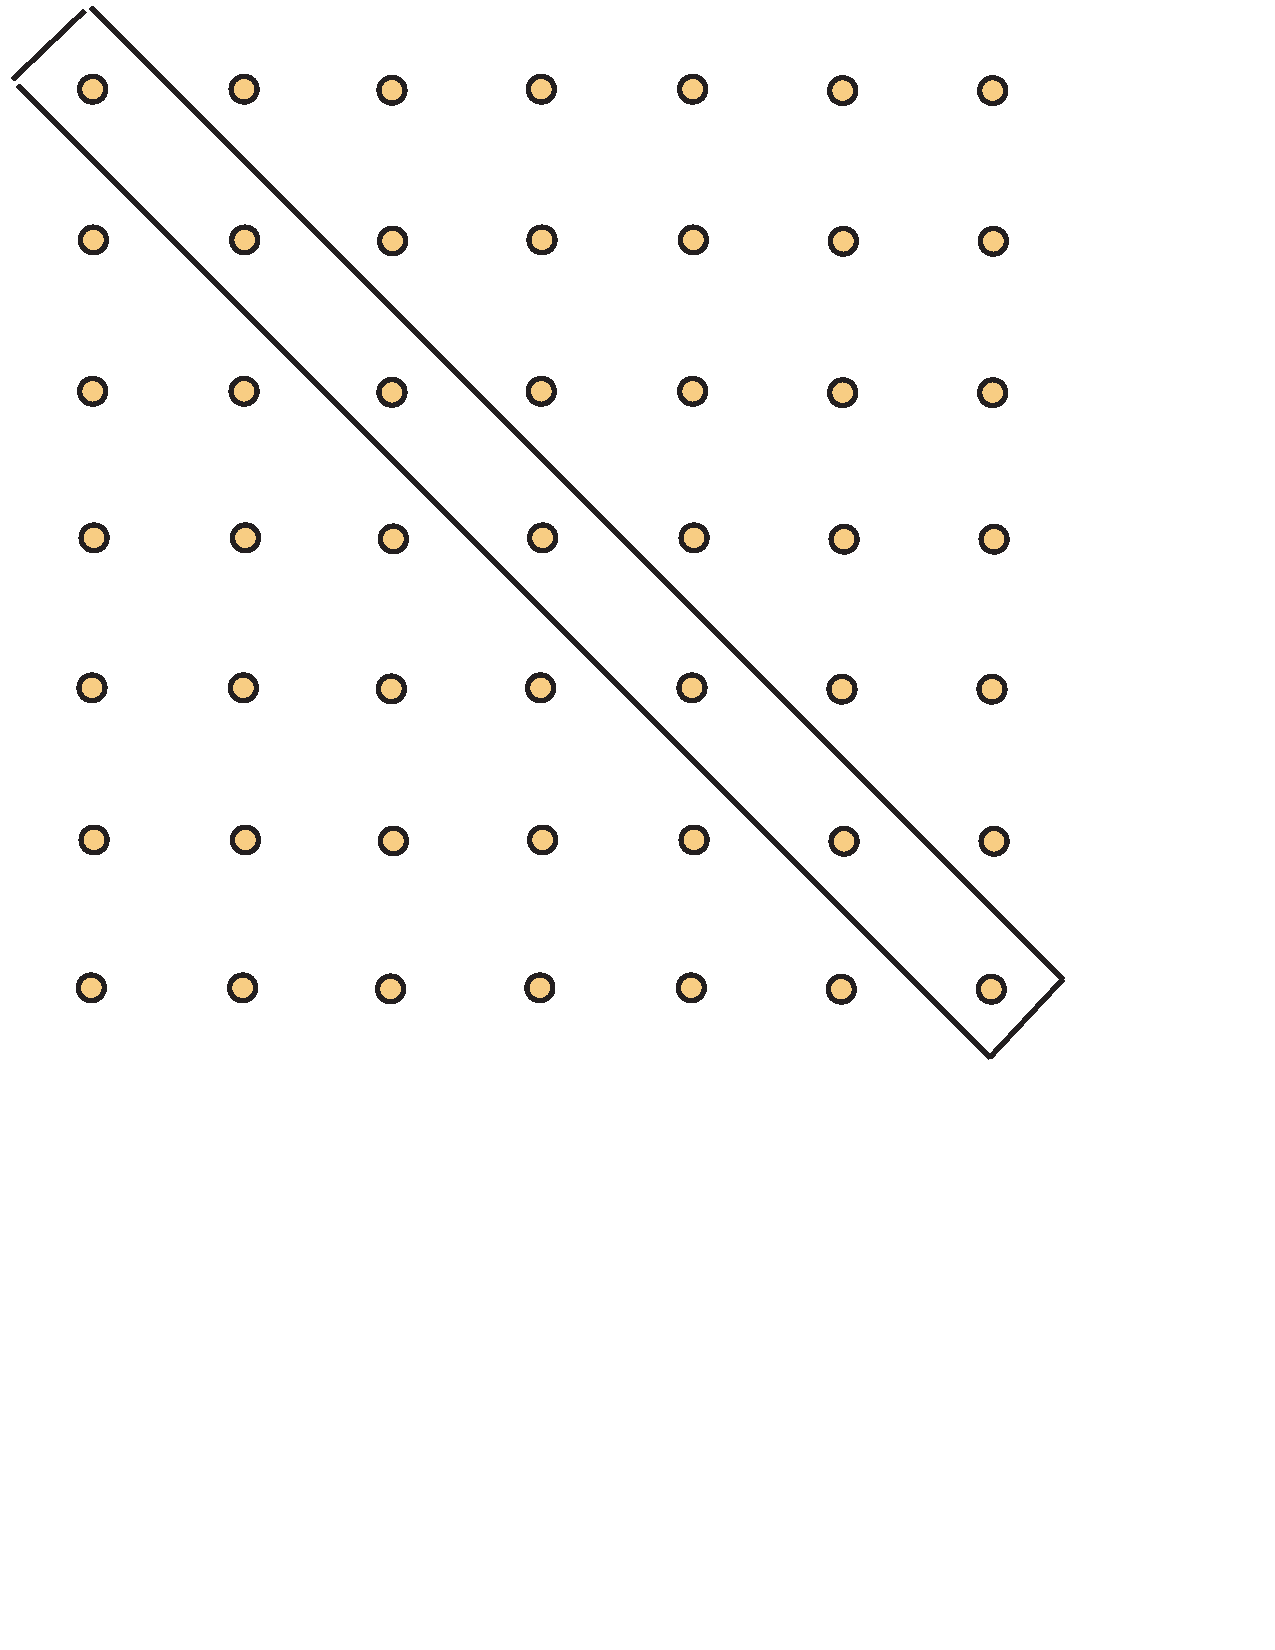
\includegraphics[scale=.3]{string-figs/3012-fig25}\\
\caption{The sum of the first $n$ integers}
\label{fig:squaredots}
\end{center}
\end{figure}


\begin{example}
Let $n$ be a positive integer. Explain why
\[
1+3+5+\dots+2n-1=n^2.
\]

The left hand side is just the
sum of the first $n$ odd integers.  But as suggested in
\autoref{fig:oddsum2}, this is clearly equal to $n^2$.

\begin{figure}
\begin{center}
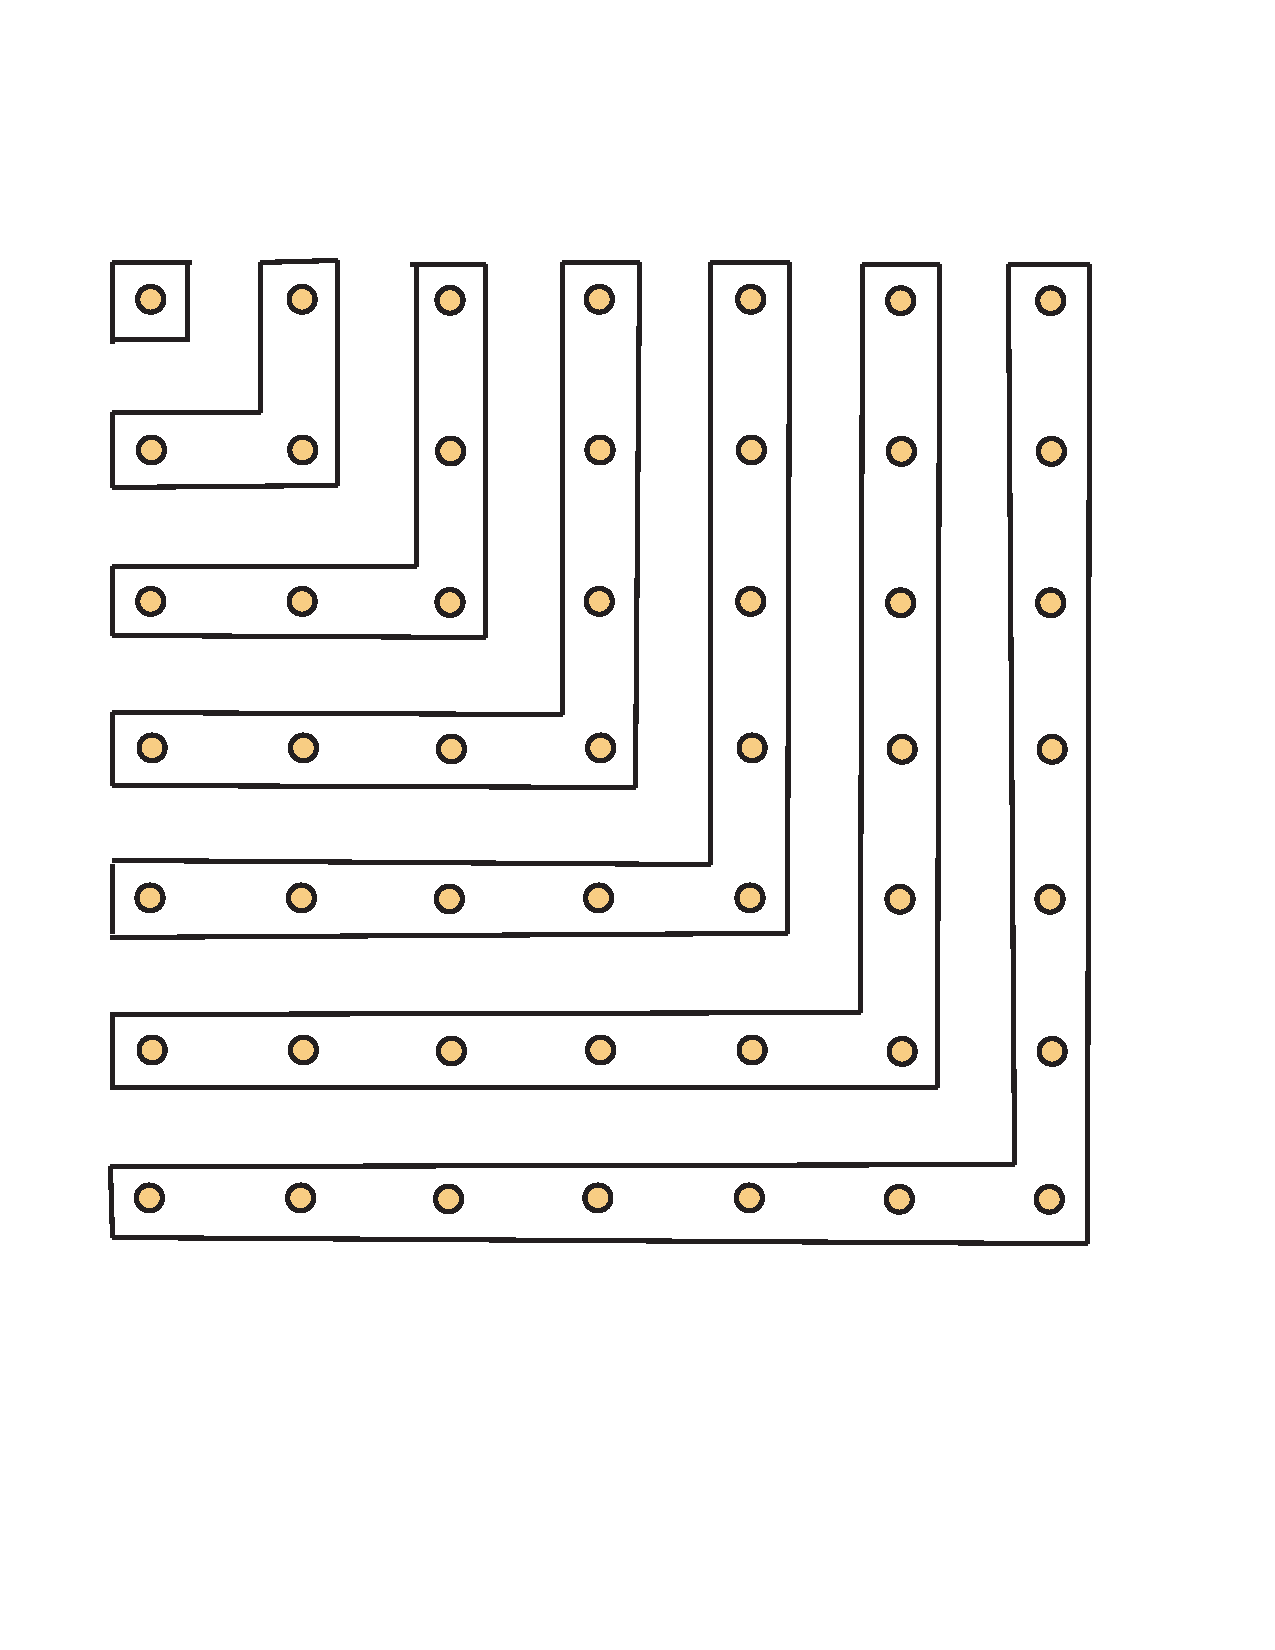
\includegraphics[scale=.3]{string-figs/3012-fig21}\\
\caption{The sum of the first $n$ odd integers
\label{fig:oddsum2}}
\end{center}
\end{figure}

\end{example}

\begin{example}
Let $n$ be a positive integer.  Explain why
\[
\binom{n}{0}+\binom{n}{1}+\binom{n}{2}+\dots+\binom{n}{n}=2^n.
\]
Both sides count the number of bit strings of length $n$, with
the left side first grouping them according to the number of
$0$'s.
\end{example}

\begin{example}
Let $n$ and $k$ be integers with $0\le k<n$.
Then
\[
\binom{n}{k+1} = \binom{k}{k} + \binom{k+1}{k} +
\binom{k+2}{k} +\dots+
\binom{n-1}{k}.
\]
To prove this formula, we simply observe that both sides count the
number of bit strings of length~$n$ that contain $k+1$ $1$'s with the
right hand side first partitioning them according to the last
occurence of a~$1$. (For example, if the last $1$ occurs in position
$k+5$, then the remaining $k$ $1$'s must appear in the preceding $k+4$
positions, giving $C(k+4,k)$ strings of this type.)  Note that
when $k=1$ (so $k+1=2$), we have the same formula as developed earlier for the
sum of the first $n$ positive integers.
\end{example}

\begin{example}
Explain the identity
\[3^n=\binom{n}{0}2^0+\binom{n}{1}2^1+\binom{n}{2}2^2+
\dots+\binom{n}{n}2^n.
\]
Both sides count the number of $\{0,1,2\}$-strings of length~$n$,
the right hand side first partitioning them according to positions
in the string which are not~$2$. (For instance, if $6$ of the
positions are not~$2$, we must first choose those $6$ positions in
$C(n,6)$ ways and then there are $2^6$ ways to fill in those six
positions by choosing either a $0$ or a $1$ for each position.)
\end{example}

\begin{example}
For each non-negative integer~$n$,
\[
\binom{2n}{n}=
{\binom{n}{0}}^2+{\binom{n}{1}}^2+{\binom{n}{2}}^2+\dots+
 {\binom{n}{n}}^2.
\]
Both sides count the number of bit strings of length $2n$ with half
the bits being $0$'s, with the right side first partitioning them
according to the number of $1$'s occurring in the first $n$ positions
of the string.  Note that we are also using the trivial identity
$\binom{n}{k}=\binom{n}{n-k}$.
\end{example}

\section{The Ubiquitous Nature of Binomial Coefficients}\label{s:strings:bin-coeff}

In this section, we present several combinatorial problems
that can be solved by appeal to binomial coefficients,
even though at first glance, they do not appear to have
anything to do with sets.

\begin{example} 
  The office assistant is distributing supplies.  In how many ways can
  he distribute 18 identical folders among four office employees:
  Audrey, Bart, Cecilia and Darren, with the additional restriction that
  each will receive at least one folder?

  Imagine the folders placed in a row.  Then there are 17 gaps between
  them.  Of these gaps, choose three and place a divider in each.
  Then this choice divides the folders into four non-empty sets.  The
  first goes to Audrey, the second to Bart, etc.  Thus the answer is
  $C(17,3)$.  In Figure~\ref{fig:distrib}, we illustrate this scheme
  with Audrey receiving~$6$ folders, Bart getting~$1$, Cecilia~$4$ and
  Darren~7.

\begin{figure}
\begin{center}
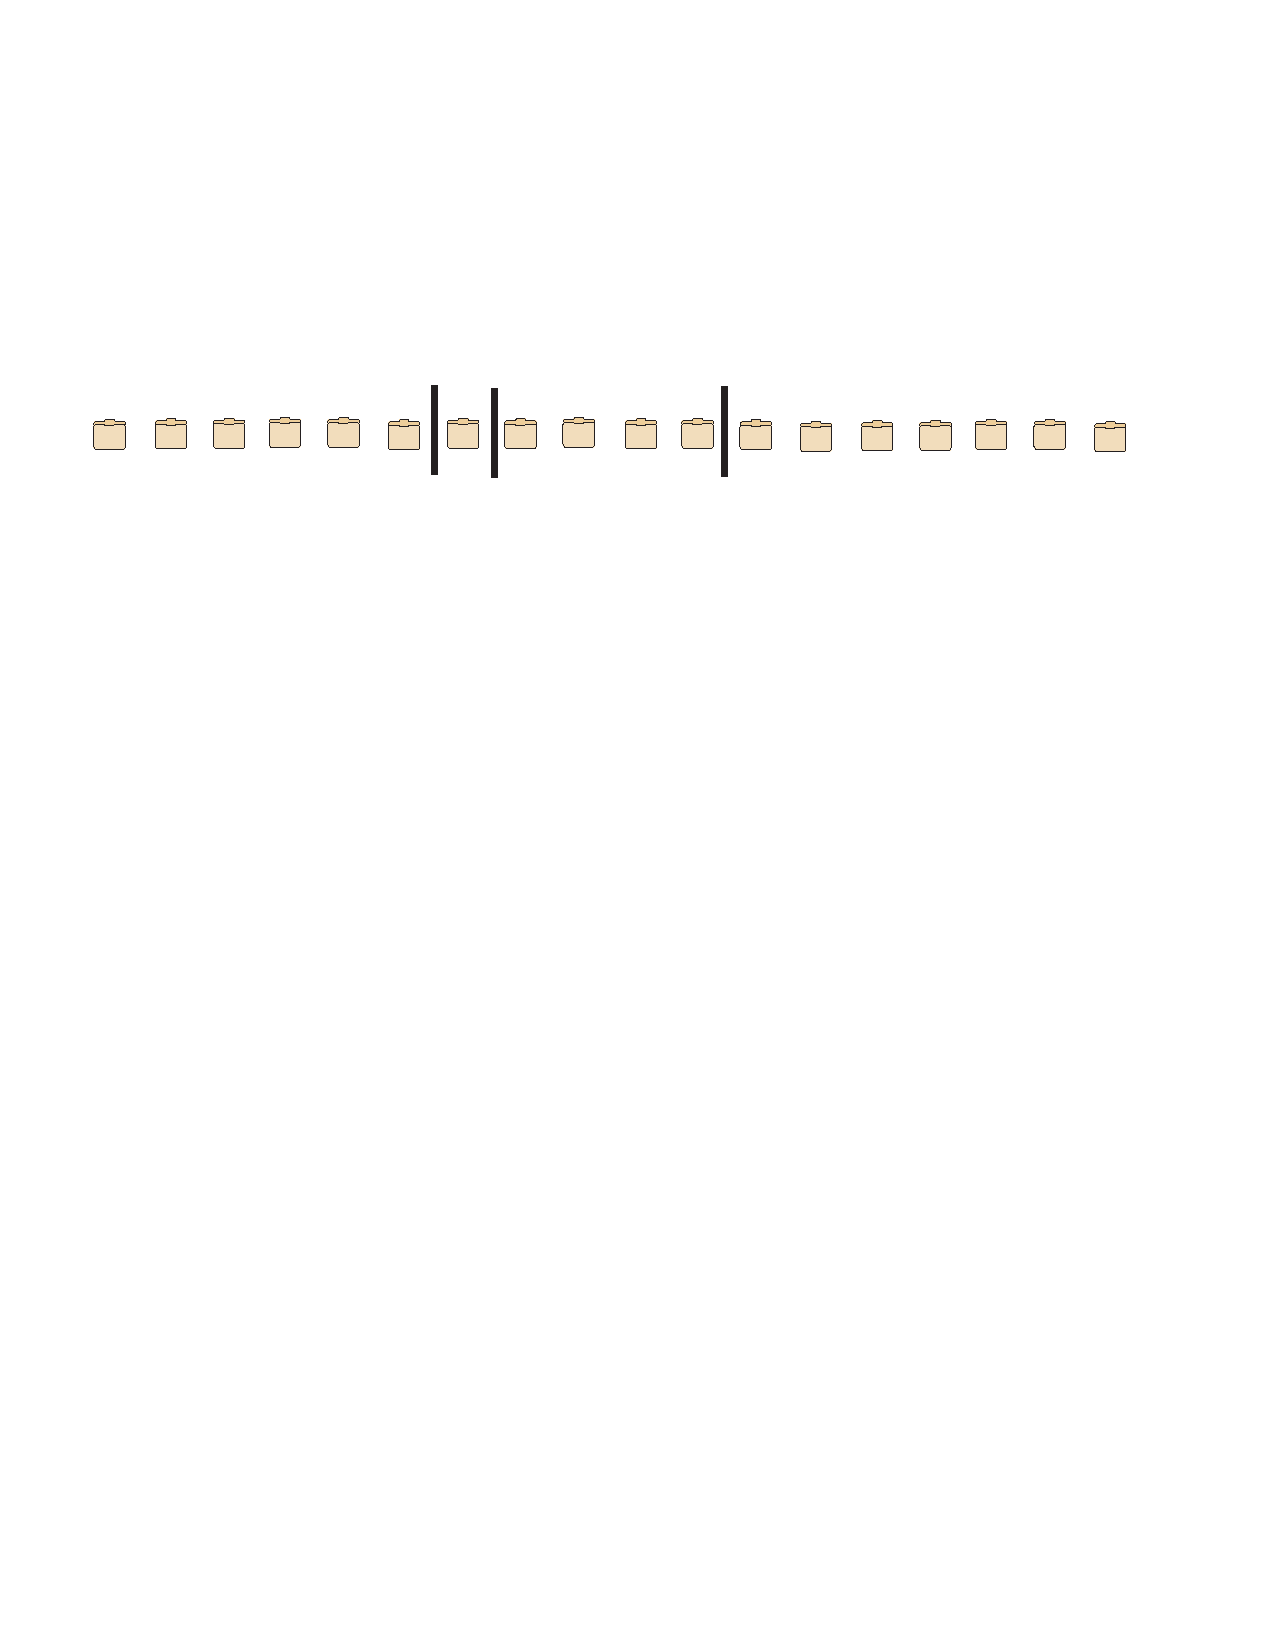
\includegraphics[scale=.6]{string-figs/3012-fig23}
\caption{{Distributing Identical Objects into Distinct
    Cells}}
\label{fig:distrib}
\end{center}
\end{figure}
\end{example}

\begin{example}
Suppose we redo the preceding problem but drop the restriction
that each of the four employees gets at least one folder.  
Now how many ways can the distribution be made?

The solution involves a ``trick'' of sorts.  First, we convert the
problem to one that we already know how to solve.  This is
accomplished by \textit{artificially} inflating everyone's allocation
by one.  In other words, if Bart will get $7$ folders, we say that he
will get $8$.  Also, artificially inflate the number of folders by
$4$, one for each of the four persons.  So now imagine a row of
$22=18+4$ folders.  Again, choose $3$ gaps.  This determines a
non-zero allocation for each person.  The actual allocation is one
less---and may be zero.  So the answer is $C(21,3)$.
\end{example}

\begin{example}
  Again we have the same problem as before, but now we want to count
  the number of distributions where only Audrey and Cecilia are
  guaranteed to get a folder. Bart and Darren are allowed to get zero
  folders.  Now the trick is to artificially inflate Bart and Darren's
  allocation, but leave the numbers for Audrey and Cecilia as is.  So
  the answer is $C(19,3)$.
\end{example}

\begin{example}
Here is a reformulation of the preceding discussion expressed in terms
of integer solutions of inequalities.

We count the number of integer solutions to the inequality
\[
x_1+x_2+x_3+x_4+x_5+x_6\le 538
\]
subject to various sets of restrictions on the values of
$x_1,x_2,\dots,x_6$.  Some of these restrictions will require
that the inequality actually be an equation.
 
The number of integer solutions is:

\begin{enumerate}
\item $C(537,5)$, when all $x_i> 0$ and equality holds.
\item $C(543,5)$, when all $x_i\ge 0$ and equality holds.
\item $C(291,3)$, when $x_1,x_2,x_4,x_6>0$, $x_3=52$,
$x_5=194$, and equality holds.
\item $C(537,6)$, when all $x_i > 0$ and the inequality is
strict. \textit{Hint:} Imagine a new variable $x_7$ which is
the balance.  Note that $x_7$ must be positive.
\item $C(543,6)$, when all $x_i \ge 0$ and the inequality is
strict. \textit{Hint:} Add a new variable $x_7$ as above.   Now it
is the only one which is required to be positive.
\item $C(544,6)$, when all $x_i \ge 0$.
\end{enumerate}
\end{example}

A classical enumeration problem (with connections to several problems)
involves counting lattice paths. A \textit{lattice path} in the plane
is a sequence of ordered pairs of integers:
\[
(m_1,n_1), (m_2,n_2), (m_3,n_3),\dots,(m_t,n_t)
\]
so that for all $i=1,2,\dots,t-1$, either
\begin{enumerate}
\item  $m_{i+1}=m_{i}+1$ and $n_{i+1}=n_i$, or
\item  $m_{i+1}=m_i$ and $n_{i+1}=n_{i}+1$.
\end{enumerate}

In Figure~\ref{fig:latticepath}, we show a lattice path from
$(0,0)$ to $(13,8)$.

\begin{figure}
\begin{center}
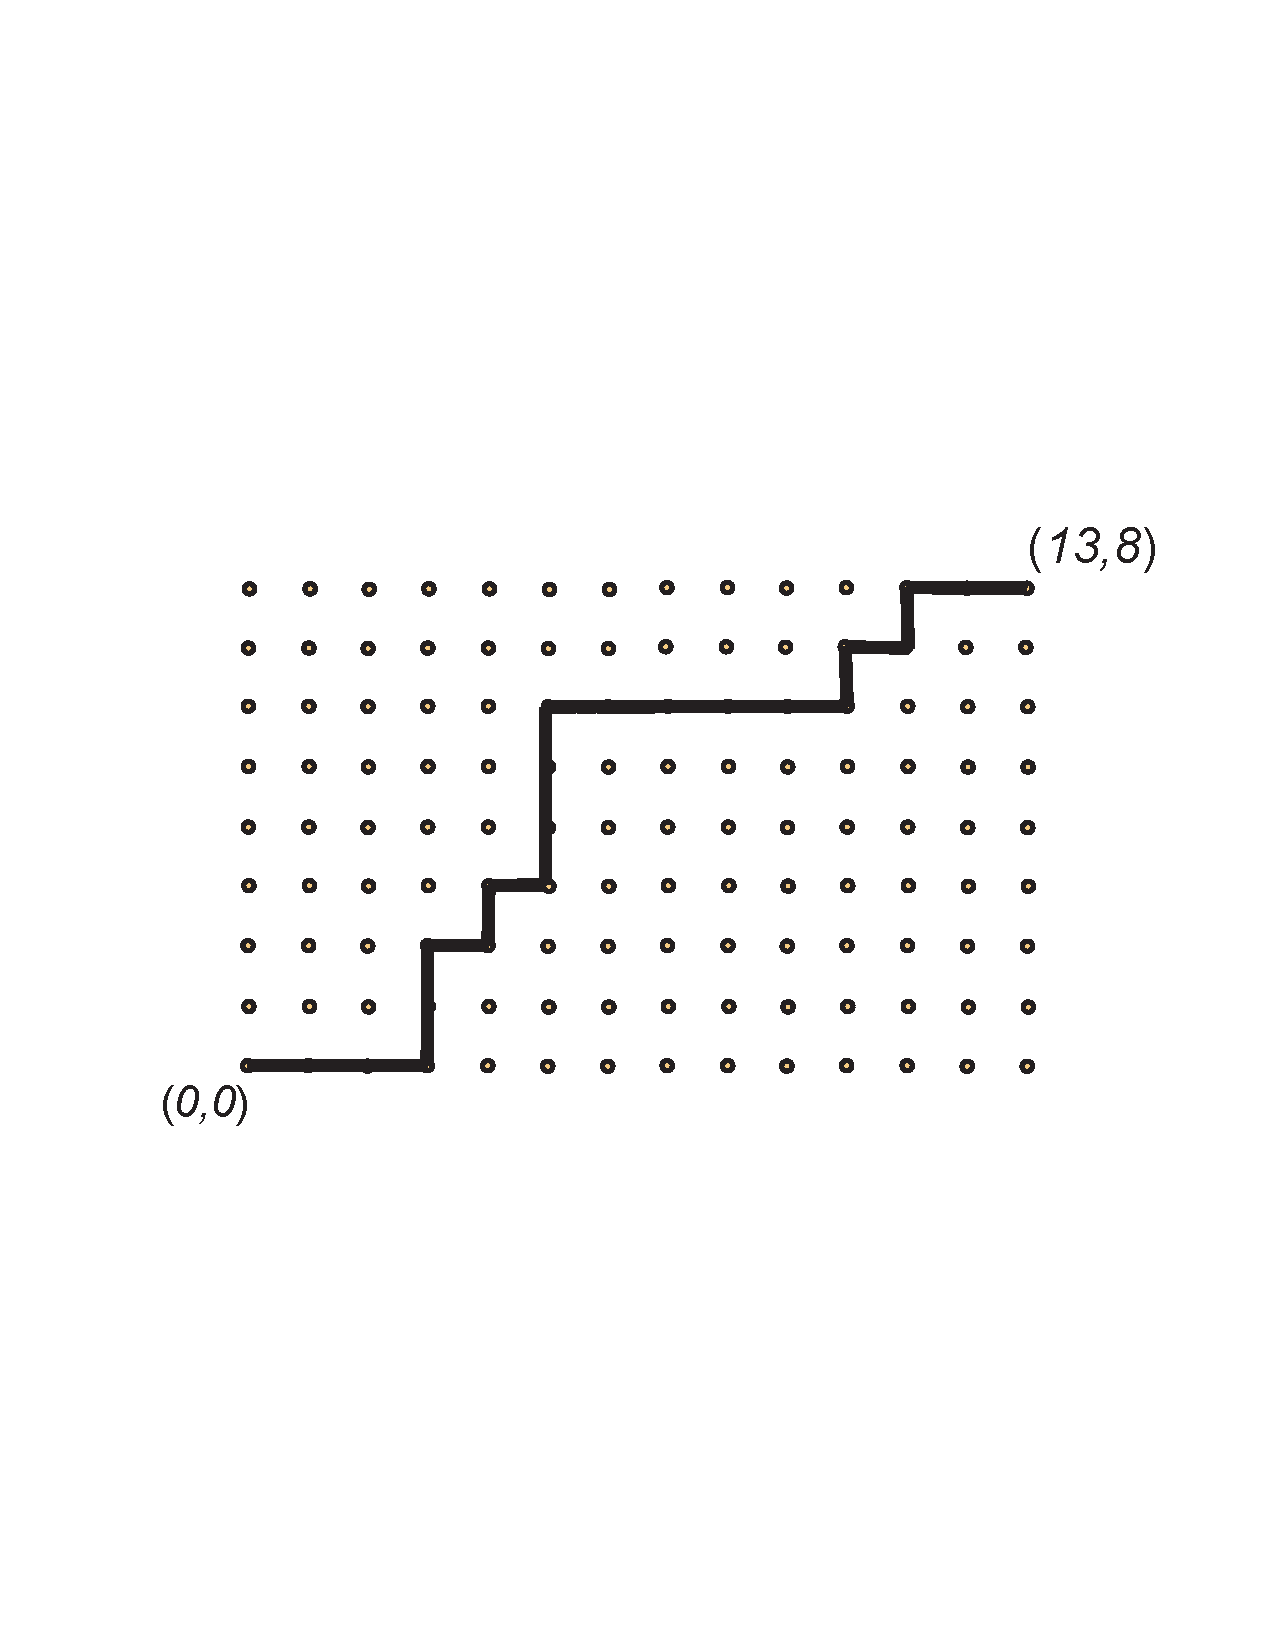
\includegraphics[scale=.4]{string-figs/3012-fig22}
\caption{A Lattice Path}
\label{fig:latticepath}
\end{center}
\end{figure}

\begin{example}  The number of lattice paths from $(m,n)$ to
$(p,q)$ is $C((p-m)+(q-n),p-m)$.

To see why this formula is valid, note that a lattice 
path is just an $X$-string with
$X=\{H,V\}$, where $H$ stands for \textit{horizontal} and $V$ stands
for \textit{vertical}.  In this case, there are exactly $(p-m)+(q-n)$
moves, of which $p-m$ are horizontal.
\end{example}

\begin{example}

Let $n$ be a non-negative integer.  Then the number of lattice
paths from $(0,0)$ to $(n,n)$ which never go above the diagonal
line $y=x$ is the Catalan number 
\[
C(n) =\frac{1}{n+1}\binom{2n}{n}.
\]

To see that this formula holds, consider the family $\cgP$ of all
lattice paths from $(0,0)$ to $(n,n)$.  A lattice path from $(0,0)$ to
$(n,n)$ is just a $\{H,V\}$-string of length $2n$ with exactly $n$
$H$'s.  So $|\cgP|=\binom{2n}{n}$.  We classify the paths in $\cgP$ as
\textit{good} if they never go over the diagonal; otherwise, they are
\textit{bad}.  A string $s\in\cgP$ is good if the number of $V$'s in
an initial segment of $s$ never exceeds the number of $H$'s.  For
example, the string ``$HHVHVVHHHVHVVV$'' is a good lattice path from
$(0,0)$ to $(7,7)$, while the path ``$HVHVHHVVVHVHHV$'' is bad.  In
the second case, note that after~$9$ moves, we have~$5$ $V$'s
and~$4$~$H$'s.

Let $\cgG$ and $\cgB$ denote the family of all good and bad paths,
respectively.  Of course, our goal is to determine $|\cgG|$.

Consider a path $s\in\cgB$. Then there is a least integer $i$ so that
$s$ has more $V$'s than $H$'s in the first $i$ positions. By the
minimality of $i$, it is easy to see that $i$ must be odd (otherwise,
we can back up a step), and if we set $i=2j+1$, then in the first
$2j+1$ positions of $s$, there are exactly $j$ $H$'s and $j+1$
$V$'s. The remaining $2n-2j-1$ positions (the ``tail of $s$'') have
$n-j$ $H$'s and $n-j-1$ $V$'s. We now transform $s$ to a new string
$s'$ by replacing the $H$'s in the tail of $s$ by $V$'s and the $V$'s
in the tail of $s$ by $H$'s and leaving the initial $2j+1$ positions
unchanged. For example, see Figure~\ref{flippath}, where the path $s$
is shown solid and $s'$ agrees with $s$ until it crosses the line
$y=x$ and then is the dashed path. Then $s'$ is a string of length
$2n$ having $(n-j)+(j+1) = n+1$ $V$'s and $(n-j-1)+j=n-1$ $H$'s, so
$s'$ is a lattice path from $(0,0)$ to $(n-1,n+1)$. Note that there
are $\binom{2n}{n-1}$ such lattice paths.

\begin{figure}
\begin{center}
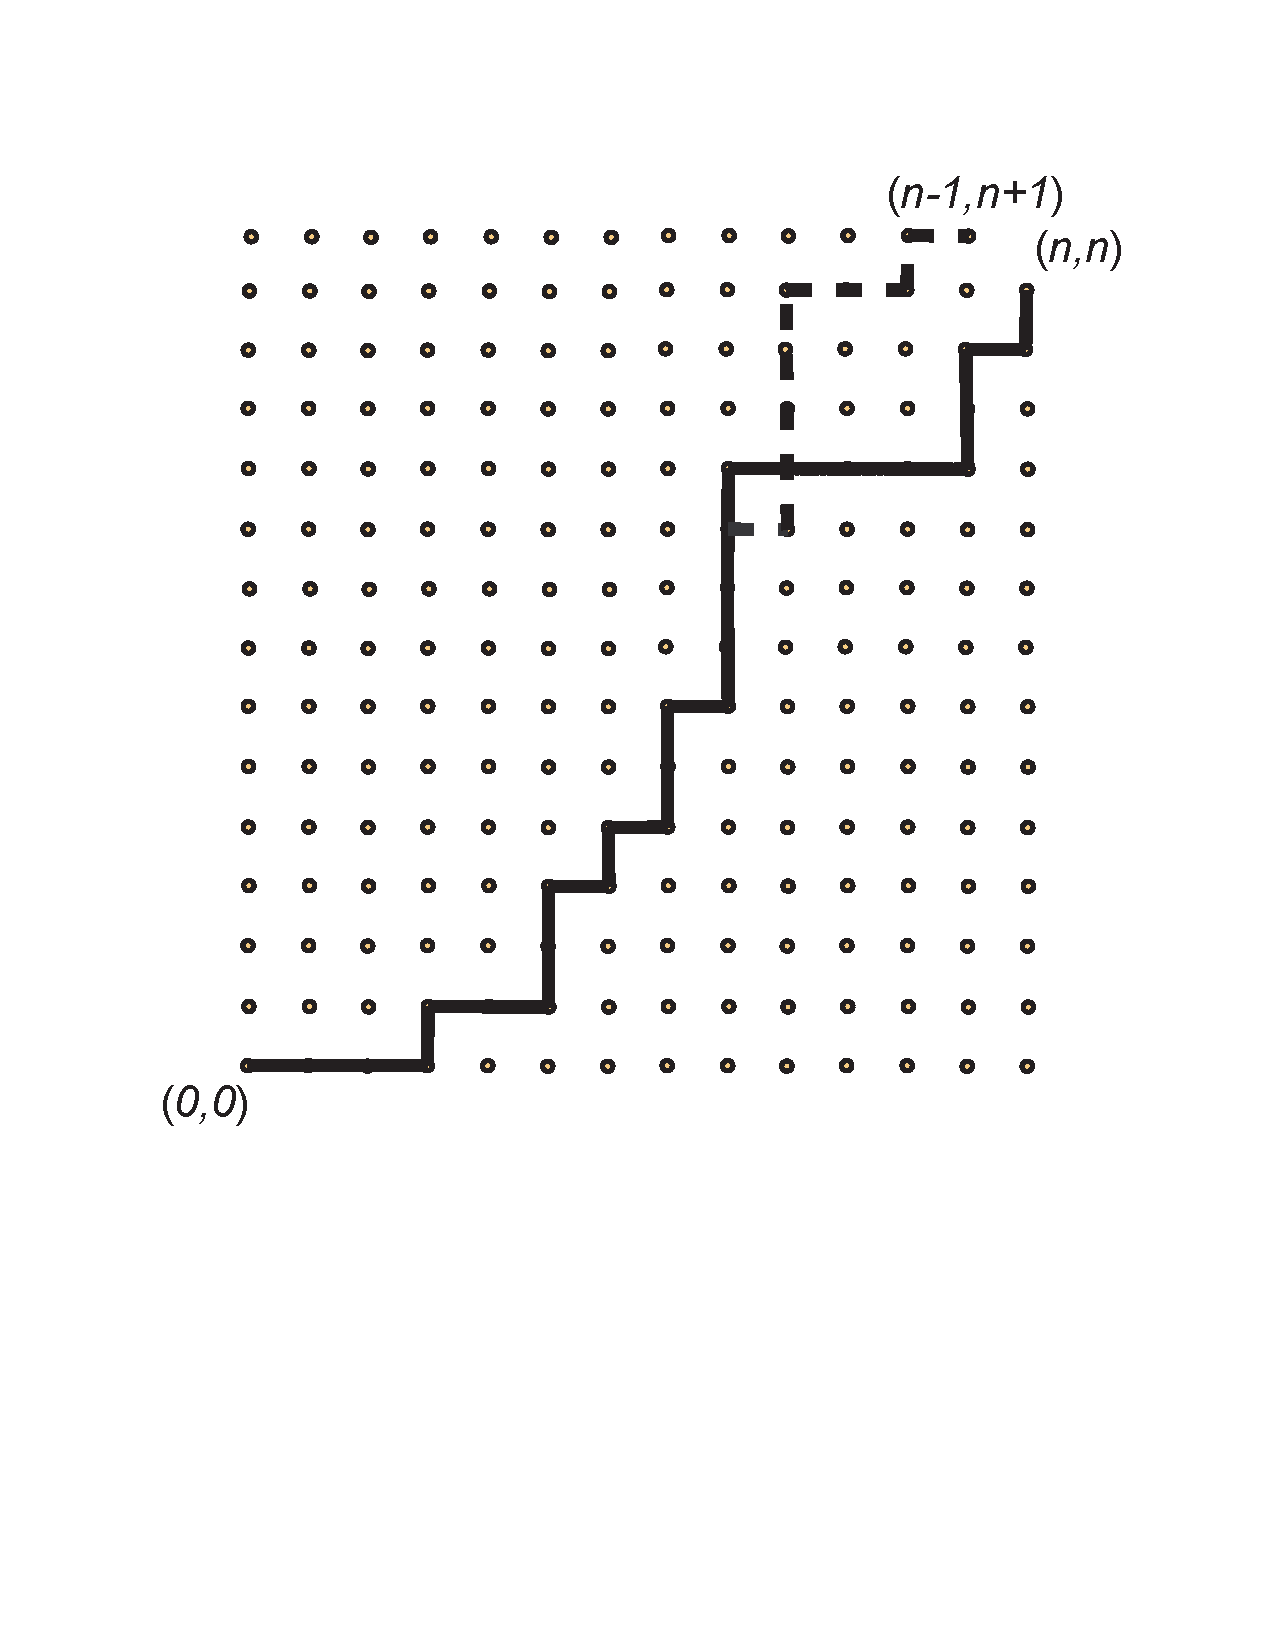
\includegraphics[scale=.4]{string-figs/3012-fig26}\\
\caption{Transforming a Lattice Path}
\label{flippath}
\end{center}
\end{figure}

We can also observe that the transformation we've described is in fact
a bijection between $\cgB$ and $\cgP'$, the set of lattice paths from
$(0,0)$ to $(n-1,n+1)$. To see that this is true, note that every path
$s'$ in $\cgP'$ must cross the line $y=x$, so there is a first time it
crosses it, say in position $i$. Again, $i$ must be odd, so $i=2j+1$
and there are $j$ $H$'s and $j+1$ $V$'s in the first $i$ positions of
$s'$. Therefore the tail of $s'$ contains $n+1-(j+1)=n-j$ $V$'s and
$(n-1)-j$ $H$'s, so interchanging $H$'s and $V$'s in the tail of $s'$
creates a new string $s$ that has $n$ $H$'s and $n$ $V$'s and thus
represents a lattice path from $(0,0)$ to $(n,n)$, but it's still a
bad lattice path, as we did not adjust the first part of the path,
which results in crossing the line $y=x$ in position $i$. Therefore,
$|\cgB|=|\cgP'|$ and thus
\[C(n)=|\cgG|=|\cgP|-|\cgB|=|\cgP|-|\cgP'| = \binom{2n}{n} -
\binom{2n}{n-1} = \frac{1}{n+1}\binom{2n}{n},\]
after a bit of algebra.
\end{example}

It is worth observing that in the preceding example, we made use of
two common enumerative techniques: giving a bijection between two
classes of objects, one of which is ``easier'' to count than the
other, and counting the objects we do \textit{not} wish to enumerate
and deducting their number from the total.

\section{The Binomial Theorem}\label{s:strings:binom-thm}

Here is a truly basic result from combinatorics kindergarten.

\begin{theorem}[Binomial Theorem]\label{thm:binomial}
Let $x$ and $y$ be real numbers with $x$, $y$ and $x+y$ non-zero.
Then for every non-negative integer $n$,
\[
(x+y)^n=\sum_{i=0}^{n}\binom{n}{i}x^{n-i}y^{i}.
\]
\end{theorem}

\begin{proof}
View $(x+y)^n$ as a product
\[ 
(x+y)^n=\underbrace{(x+y)(x+y)(x+y)(x+y)\dots(x+y)(x+y)}_{n\text{ factors}}.
\]
Each term of the expansion of the product results from choosing either
$x$ or $y$ from one of these factors.  If $x$ is chosen $n-i$ times
and $y$ is chosen $i$ times, then the resulting product is
$x^{n-i}y^i$.  Clearly, the number of such terms is $C(n,i)$, i.e.,
out of the $n$ factors, we choose the element $y$ from $i$ of them,
while we take $x$ in the remaining $n-i$.
\end{proof}

\begin{example}
  There are times when we are interested not in the full expansion of
  a power of a binomial, but just the coefficient on one of the
  terms. The Binomial Theorem gives that the coefficient of $x^5y^8$
  in $(2x-3y)^{13}$ is $\binom{13}{5}2^{5}(-3)^8$.
\end{example}

\section{Multinomial Coefficients}\label{s:strings:multinom}

Let $X$ be a set of $n$ elements.  Suppose that we have
two colors of paint, say red and blue, and we are going to
choose a subset of $k$ elements to be painted red with the
rest painted blue.  Then the number of different ways this
can be done is just the binomial coefficient $\binom{n}{k}$.
Now suppose that we have three different colors, say red,
blue, and green.  We will choose $k_1$ to be
colored red, $k_2$ to be colored blue, with the remaining
$k_3 = n - (k_1+k_2)$ colored green.  We may compute the number of
ways to do this by first choosing $k_1$ of the $n$ elements to paint
red, then from the remaining $n-k_1$ choosing $k_2$ to paint blue, and
then painting the remaining $k_3$ green. It is easy to see that 
the number of ways to do this is 
\[
\binom{n}{k_1}\binom{n-k_1}{k_2} = \frac{n!}{k_1!(n-k_1)!}
\frac{(n-k_1)!}{k_2!(n-(k_1+k_2))!} = \frac{n!}{k_1!k_2!k_3!}
\]
Numbers of this form are called \textit{multinomial coefficients};
they are an obvious generalization of the binomial coefficients.
The general notation is:

\[
\binom{n}{k_1,k_2,k_3,\dots,k_r}=\frac{n!}{k_1!k_2!k_3!\dots k_r!}.
\]
For example, 
\[
\binom{8}{3,2,1,2}=\frac{8!}{3!2!1!2!}= 
  \frac{40320}{6\cdot2\cdot1\cdot2}=1680.
\]
Note that there is some ``overkill'' in this notation, since
the value of $k_r$ is determined by $n$ and the values for
$k_1$, $k_2,\dots,k_{r-1}$.  For example, with the ordinary
binomial coeffients, we just write $\binom{8}{3}$ and not
$\binom{8}{3,5}$.

\begin{example} 
How many different rearrangements of the string:
\[
\text{MITCHELTKELLERANDWILLIAMTTROTTERAREREGENIUSES!!}
\]
are possible if all letters and characters must be used?

To answer this question, we note that there are a total of $45$
characters distributed as follows: 3~A's, 1~C, 1~D, 7~E's, 1~G, 1~H,
4~I's, 1~K, 5~L's, 2~M's, 2~N's, 1~O, 4~R's, 2~S's, 6~T's, 1~U, 1~W,
and 2~!'s.  So the number of rearrangements is
\[
\frac{45!}{3!1!1!7!1!1!4!1!5!2!2!1!4!2!6!1!1!2!}.
\]
\end{example}

Just as with binomial coefficients and the Binomial Theorem, the
multinomial coefficients arise in the expansion of powers of a
multinomial:

\begin{theorem}[Multinomial Theorem]
  Let $x_1, x_2, \dots, x_r$ be nonzero real numbers with
  $\sum_{i=1}^r x_i\neq 0$. Then for every $n\in \nni$,
  \[(x_1+x_2+\cdots + x_r)^n =
  \sum_{k_1+k_2+\cdots+k_r=n}\binom{n}{k_1,k_2,\dots,k_r}
  x_1^{k_1}x_2^{k_2}\cdots x_r^{k_r}.\]
\end{theorem}

\begin{example}
  What is the coefficient of $x^{99}y^{60}z^{14}$ in
  $(2x^3+y-z^2)^{100}$? What about $x^{99}y^{61}z^{13}$?

  By the Multinomial Theorem, the expansion of $(2x^3+y-z^2)^{100}$
  has terms of the form
  \[\binom{100}{k_1,k_2,k_3} (2x^3)^{k_1}y^{k_2}(-z^2)^{k_3} =
  \binom{100}{k_1,k_2,k_3} 2^{k_1}x^{3k_1}y^{k_2}(-1)^{k_3}z^{2k_3}.\]
  The $x^{99}y^{60}z^{14}$ arises when $k_1 = 33$, $k_2=60$, and
  $k_3=7$, so it must have coefficient
  \[-\binom{100}{33,60,7}2^{33}.\]

  For $x^{99}y^{61}z^{13}$, the exponent on $z$ is odd, which cannot
  arise in the expansion of $(2x^3+y-z^2)^{100}$, so the coefficient
  is $0$.
\end{example}

\section{Discussion}

Over coffee, Xing said that he had been experimenting with
the Maple software discussed in the introductory chapter.
He understood that Maple was treating a big integer as a string.
Xing enthusiastically reported that he had asked Maple to
find the sum $a+b$ of two large integers $a$ and $b$, each having more
than $800$ digits.  Maple found the answer about as fast as he
could hit the enter key on his netbook. 
``That's not so impressive'' Alice interjected.
``A human, even Bob, could do this in a couple of minutes using
pencil and paper.''  ``Thanks for your kind remarks,'' replied Bob,
with the rest of  the group noting that that Alice was being pretty
harsh on Bob and not for any good reason.

Dave took up Bob's case with the remark that ``Very few humans, not
even you Alice, would want to tackle finding the product of $a$ and
$b$ by hand.''  Xing jumped back in with ``That's the point.  Even
a tiny netbook can find the product very, very quickly.  In fact, I tried
it out with two integers, each having more than one thousand
digits.  It found the product in about one second.''  Ever the
skeptic, Zori said ``You mean you carefully typed in two
integers of that size?''  Xing quickly replied ``Of course not.  I
just copied and pasted the data from one source to another.''
Yolanda said ``What a neat trick that is.  Really cuts down the
chance of an error.''

Dave said ``What about factoring?  Can your netbook with its
fancy software for strings factor big integers?''  Xing
said that he would try some sample problems and report back.  
Carlos said  ``Factoring an integer with several hundred digits is
likely to be very challenging, not only for a netbook, but also for
a super computer.  For example, suppose the given integer was
either a prime or the product of two large primes.  Detecting
which of these two statements holds could be very difficult.''

Undeterred, Dave continued ''What about exponentiation?  Can your
software calculate $a^b$ when $a$ and $b$ are large integers?''
Xing said ``That shouldn't be a problem.  After all, $a^b$ is just
multiplying $a$ times itself a total of $b$ times, and if you
can do multiplication quickly, that's just a loop.''  Yolanda said
that the way Xing was describing things, he was actually
talking about a program with nested loops so it might take a long time 
for such a program to halt.  Carlos was quiet but he thought
there might be ways to speed up such computations.

By this time, Alice reinserted herself into the conversation ``Hey guys.
While you were talking, I was looking for big integer topics on the
web and found this problem.  Is $838200020310007224300$ a Catalan number?
How would you answer this?  Do you have to use special software?''

Zori was not happy.  She gloomily envisioned a future job hunt
in which she was compelled to use big integer arithmetic as a job skill.  Arrgghh.

\section{Exercises}\label{s:strings:exercises}
  \begin{enumerate}
  \item The Hawaiian alphabet consists of $12$ letters. How many
    six-character strings can be made using the Hawaiian alphabet?
  \item How many $2n$-digit positive integers can be formed if the
    digits in odd positions (counting the rightmost digit as position
    $1$) must be odd and the digits in even positions must be even and
    positive?
  \item Matt is designing a website authentication system. He knows
    passwords are most secure if they contain letters, numbers, and
    symbols. However, he doesn't quite understand that this additional
    security is defeated if he specifies in which positions each
    character type appears. He decides that valid passwords for his
    system will begin with three letters (uppercase and lowercase both
    allowed), followed by two digits, followed by one of $10$ symbols,
    followed by two uppercase letters, followed by a digit, followed
    by one of $10$ symbols. How many different passwords are there for
    his website system? How does this compare to the total number of
    strings of length $10$ made from the alphabet of all uppercase and
    lowercase English letters, decimal digits, and $10$ symbols?
  \item How many ternary strings of length $2n$ are there in which the
    zeroes appear only in odd-numbered positions?
  \item Suppose we are making license plates of the form
    $l_1l_2l_3-d_1d_2d_3$ where $l_1,l_2,l_3$ are capital letters in
    the English alphabet and $d_1,d_2,d_3$ are decimal digits (i.e.,
    in $\{0,1,2,3,4,5,6,7,8,9\}$) subject to the restriction that at
    least one digit is nonzero and at least one letter is $K$. How
    many license plates can we make?
  \item Mrs.\ Steffen's third grade class has $30$ students in it. The students
    are divided into three groups (numbered $1$, $2$, and $3$), each
    having $10$ students.
    \begin{enumerate}
    \item The students in group $1$ earned $10$ extra minutes of
      recess by winning a class competition. Before going out for
      their extra recess time, they form a single file line. In how
      many ways can they line up?
    \item When all $30$ students come in from recess together, they
      again form a single file line. However, this time the students
      are arranged so that the first student is from group $1$, the
      second from group $2$, the third from group $3$, and from there
      on, the students continue to alternate by group in this
      order. In how many ways can they line up to come in from recess?
    \end{enumerate}
  \item How many strings of the form $l_1l_2d_1d_2d_3l_3l_4d_4l_5l_6$
    are there where
    \begin{itemize}
    \item for $1\leq i\leq 6$, $l_i$ is an uppercase letter in the
      English alphabet;
    \item for $1\leq i\leq 4$, $d_i$ is a decimal digit;
    \item $l_2$ is not a vowel (i.e., $l_2\nin\{\text{A,E,I,O,U}\}$); and
    \item the digits $d_1$, $d_2$, and $d_3$ are distinct (i.e.,
      $d_1\neq d_2\neq d_3\neq d_1$).
    \end{itemize}
  \item In this exercise, we consider strings made from uppercase
    letters in the English alphabet and decimal digits. How many
    strings of length $10$ can be constructed in each of the following
    scenarios?
    \begin{enumerate}
    \item The first and last characters of the string are letters.
    \item The first character is a vowel, the second character is a
      consonant, and the last character is a digit.
    \item Vowels (not necessarily distinct) appear in the third,
      sixth, and eighth positions and no other positions.
    \item Vowels (not necessarily distinct) appear in exactly two
      positions.
    \item Precisely four characters in the string are digits and no
      digit appears more than one time.
    \end{enumerate}
  \item A database uses $20$-character strings as record
    identifiers. The valid characters in these strings are upper-case
    letters in the English alphabet and decimal digits. (Recall there
    are $26$ letters in the English alphabet and $10$ decimal digits.)
    How many valid record identifiers are possible if a valid record
    identifier must meet \emph{all} of the following criteria:
    \begin{itemize}
    \item Letter(s) from the set $\{A,E,I,O,U\}$ occur in
      \emph{exactly} three positions of the string.
    \item The last three characters in the string are \emph{distinct}
      decimal digits that do not appear elsewhere in the string.
    \item The remaining characters of the string may be filled with
      any of the remaining letters or decimal digits.
    \end{itemize}
  \item Let $X$ be the set of the $26$ lowercase English letters and
    $10$ decimal digits. How many $X$-strings of length $15$
    satisfy \emph{all} of the following properties (at the same time)?
    \begin{itemize}
    \item The first and last symbols of the string are distinct digits
      (which may appear elsewhere in the string).
    \item Precisely four of the symbols in the string are the letter '$t$'.
    \item Precisely three characters in the string are elements of the
      set $V=\{a,e,i,o,u\}$ and these characters are all distinct.
    \end{itemize}
  \item A donut shop sells 12 types of donuts. A manager wants to buy
    six donuts, one each for himself and his five employees.
    \begin{enumerate}
    \item Suppose that he does this by selecting a specific type of
      donut for each person. (He can select the same type of donut for
      more than one person.) In how many ways can he do this?
    \item How many ways could he select the donuts if he wants to
      ensure that he chooses a different type of donut for each
      person?
    \item Suppose instead that he wishes to select one donut of each
      of six \emph{different} types and place them in the
      breakroom. In how many ways can he do this? (The order of the
      donuts in the box is irrelevant.)
    \end{enumerate}
  \item The sport of korfball is played by teams of eight
    players. Each team has four men and four women on it. Halliday
    High School has seven men and $11$ women interested in playing
    korfball. In how many ways can they form a korfball team from their
    18 interested students?
  \item Twenty students compete in a programming competition in which
    the top four students are recognized with trophies for first,
    second, third, and fourth places.
    \begin{enumerate}
    \item How many different outcomes are there for the top four
      places?
    \item At the last minute, the judges decide that they will award
      honorable mention certificates to four individuals who did not
      receive trophies. In how many ways can the honorable mention
      recipients be selected (after the top four places have been
      determined)? How many total outcomes (trophies plus
      certificates) are there then?
    \end{enumerate}
  \item An ice cream shop has a special on banana splits, and Xing is
    taking advantage of it. He's astounded at all the options he has
    in constructing his banana split:
    \begin{itemize}
    \item He must choose three different flavors of ice cream to place
      in the asymmetric bowl the banana split is served in. The shop
      has 20 flavors of ice cream available.
    \item Each scoop of ice cream must be topped by a sauce, chosen
      from six different options. Xing is free to put the same type of
      sauce on more than one scoop of ice cream.
    \item There are $10$ sprinkled toppings available, and he must
      choose three of them to have sprinkled over the entire banana
      split.
    \end{itemize}
    \begin{enumerate}
    \item How many different ways are there for Xing to construct a
      banana split at this ice cream shop?
    \item Suppose that instead of requiring that Xing choose exactly
      three sprinkled toppings, he is allowed to choose between zero
      and three sprinkled toppings. In this scenario, how many
      different ways are there for him to construct a banana split?
    \end{enumerate}
 \item Suppose that a teacher wishes to distribute $25$ identical
    pencils to Ahmed, Barbara, Casper, and Dieter such that Ahmed and
    Dieter receive at least one pencil each, Casper receives no more
    than five pencils, and Barbara receives at least four pencils. In
    how many ways can such a distribution be made?
  \item How many integer-valued solutions are there to each of the
    following equations and inequalities?
    \begin{enumerate}
    \item $x_1+x_2+x_3+x_4+x_5=63$, all $x_i>0$
    \item $x_1+x_2+x_3+x_4+x_5=63$, all $x_i\geq 0$
    \item $x_1+x_2+x_3+x_4+x_5\leq 63$, all $x_i\geq 0$
    \item $x_1+x_2+x_3+x_4+x_5=63$, all $x_i\geq 0$, $x_2\geq 10$
    \item $x_1+x_2+x_3+x_4+x_5=63$, all $x_i\geq 0$, $x_2\leq 9$
    \end{enumerate}
  \item How many integer solutions are there to the equation
    \[x_1+x_2+x_3+x_4 = 132\]
    provided that $x_1>0$, and $x_2,x_3,x_4\geq 0$? What if we add the
    restriction that $x_4<17$?
  \item How many integer solutions are there to the inequality
    \[x_1+x_2+x_3+x_4+x_5\leq 782\] provided that
    $x_1,x_2>0$, $x_3\geq 0$, and $x_4,x_5\geq 10$?
  \item A teacher has $450$ identical pieces of candy. He wants to
    distribute them to his class of $65$ students, although he is
    willing to take some leftover candy home. (He does not insist on
    taking any candy home, however.) The student who won a contest in
    the last class is to receive at least $10$ pieces of candy as a
    reward. Of the remaining students, $34$ of them insist on
    receiving at least one piece of candy, while the remaining $30$
    students are willing to receive no candy.
    \begin{enumerate}
    \item In how many ways can he distribute the candy?
    \item In how many ways can he distribute the candy if, in addition
      to the conditions above, one of his students is diabetic and can
      receive at most $7$ pieces of candy?  (This student is one of
      the $34$ who insist on receiving at least one piece of candy.)
   \end{enumerate}
  \item Give a combinatorial argument to prove the identity
    \[k\binom{n}{k} = n\binom{n-1}{k-1}.\] \textit{Hint}: Think of
    choosing a team with a captain.
  \item Let $m$ and $w$ be positive integers. Give a combinatorial
    argument to prove that for integers $k\geq 0$,
    \[\sum_{j=0}^k \binom{m}{j}\binom{w}{k-j} = \binom{m+w}{k}.\]
  \item How many lattice paths are there from $(0,0)$ to $(10,12)$?
  \item How many lattice paths are there from $(3,5)$ to $(10,12)$?
  \item How many lattice paths are there from $(0,0)$ to $(10,12)$
    that pass through $(3,5)$?
  \item How many lattice paths from $(0,0)$ to $(17,12)$ are there
    that pass through $(7,6)$ and $(12,9)$?
  \item How many lattice paths from $(0,0)$ to $(14,73)$ are there
    that do \textit{not} pass through $(6,37)$?
  \item A small-town bank robber is driving his getaway car from the
    bank he just robbed to his hideout. The bank is at the
    intersection of $1^\text{st}$ Street and $1^\text{st}$ Avenue. He
    needs to return to his hideout at the intersection of
    $7^\text{th}$ Street and $5^\text{th}$ Avenue. However, one of his
    lookouts has reported that the town's one police officer is parked
    at the intersection of $4^\text{th}$ Street and $4^\text{th}$
    Avenue. Assuming that the bank robber does not want to get
    arrested and drives only on streets and avenues, in how many ways
    can he safely return to his hideout?  (Streets and avenues are
    uniformly spaced and numbered consecutively in this small town.)
  \item The setting for this problem is the fictional town of
    Mascotville, which is laid out as a grid. Mascots are allowed to
    travel only on the streets, and not ``as the yellow jacket
    flies.''  Buzz, the Georgia Tech mascot, wants to go visit his
    friend Thundar, the North Dakota State University mascot, who
    lives $6$ blocks east and $7$ blocks north of Buzz's
    hive. However, Uga VIII has recently moved into the doghouse $2$
    blocks east and $3$ blocks north of Buzz's hive and already has a
    restraining order against Buzz. There's also a pair of tigers (mother
    and cub) from
    Clemson who live $1$ block east and $2$ blocks north of Uga VIII,
    and they're known for setting traps for Buzz. Buzz wants to travel
    from his hive to Thundar's pen every day without encountering Uga
    VIII or The Tiger and The Tiger Cub. However, he wants to avoid
    the boredom caused by using a route he's used in the past. What is
    the largest number of consecutive days on which Buzz can make the
    trip to visit Thundar without reusing a route (you may assume
    the routes taken by Buzz only go east and north)?
  \item Determine the coefficient on $x^{15}y^{120}z^{25}$ in
    $(2x+3y^2+z)^{100}$.
    % Answer: 2^{15}3^{60}\binom{100}{15,60,25}
  \item Determine the coefficient on $x^{12}y^{24}$ in
    $(x^3+2xy^2+y+3)^{18}$. (Be careful, as $x$ and $y$ now appear in
    multiple terms!)
  \item For each word below, determine the number of rearrangements of
    the word in which all letters must be used.
    \begin{enumerate}
    \item OVERNUMEROUSNESSES
    \item OPHTHALMOOTORHINOLARYNGOLOGY
    \item HONORIFICABILITUDINITATIBUS (the longest word in the English
      language consisting strictly of alternating consonants and vowels\footnote{\url{http://www.rinkworks.com/words/oddities.shtml}})
    \end{enumerate}
  \item How many ways are there to paint a set of $27$ elements such
    that $7$ are painted white, $6$ are painted old gold, $2$ are
    painted blue, $7$ are painted yellow, $5$ are painted green, and
    $0$ of are painted red?
  \item There are many useful sets that are enumerated by the Catalan
    numbers. (Volume two of R.P.~Stanley's \emph{Enumerative
      Combinatorics} contains a famous (or perhaps infamous) exercise
    in $66$ parts asking readers to find bijections that will show
    that the number of various combinatorial structures is $C(n)$, and
    his \href{http://www-math.mit.edu/~rstan/ec/catadd.pdf}{web page}
    boasts an additional list of at least $100$ parts.) Give bijective
    arguments to show that each class of objects below is enumerated
    by $C(n)$. (All three were selected from the list in Stanley's
    book.)
    \begin{enumerate}
    \item The number of ways to fully-parenthesize a product of $n+1$
      factors as if the ``multiplication'' operation in question were
      not necessarily associative. For example, there is one way to
      parenthesize a product of two factors $(a_1a_2)$, there are two
      ways to parenthesize a product of three factors ($(a_1(a_2a_3))$
      and $((a_1a_2)a_3)$), and there are five ways to parenthesize a
      product of four factors: \[(a_1(a_2(a_3a_4))),
      (a_1((a_2a_3)a_4)), ((a_1a_2)(a_3a_4)),
      ((a_1(a_2a_3))a_4), (((a_1a_2)a_3)a_4).\]
    \item Sequences of $n$ $1$'s and $n$ $-1$'s in which the sum of
      the first $i$ terms is nonnegative for all $i$.
    \item Sequences $1\leq a_1\leq \cdots \leq a_n$ of integers with
      $a_i\leq i$. For example, for $n=3$, the sequences are
      \[111\qquad 112\qquad 113\qquad 122\qquad 123.\] \textit{Hint}:
      Think about drawing lattice paths on paper with grid lines and
      (basically) the number of boxes below a lattice path in a
      particular column.
  \end{enumerate}

\end{enumerate}


%%% Local Variables: 
%%% mode: latex
%%% TeX-master: "book"
%%% End: 

% induction.tex
% Updated January 11, 2012

\chapter{Induction}\label{ch:induction}
The twin concepts of recursion and induction are fundamentally
important in combinatorial mathematics and computer science.  In this
chapter, we give a number of examples of how recursive formulas arise
naturally in combinatorial problems, and we explain how they can be
used to make computations.  We also introduce the Principle of
Mathematical Induction and give several examples of how it is applied
to prove combinatorial statements.  Our treatment will also include
some code snippets that illustrate how functions are defined
recursively in computer programs.


\section{Introduction}\label{s:induction:intro}
A professor decides to liven up the next combinatorics class by
giving a door prize.  As students enter class (on time, because to be
late is a bit insensitive to the rest of the class), they draw a
ticket from a box.  On each ticket, a positive integer has been
printed.  No information about the range of ticket numbers is given,
although they are guaranteed to be distinct. The box of tickets was
shaken robustly before the drawing, so the contents are thoroughly mixed, 
and the selection is done without looking inside the box.

After each student has selected a ticket, the professor announces that
a cash prize of one dollar (this is a university, you know) will be
awarded to the student holding the lowest numbered ticket---from among
those drawn.

Must the prize be awarded?  In other words, given a set of positive
integers, in this case the set of ticket numbers chosen by the
students, must there be a least one?  More generally, is it true that
in any set of positive integers, there is always a least one?  What
happens if there is an enrollment surge and there are infinitely many
students in the class and each has a ticket?

\section{The Positive Integers are Well Ordered}\label{s:induction:posintsord}

Most likely, you answered the questions posed above with an
enthusiastic ``yes'', in part because you wanted the shot at the
money, but more concretely because it seems so natural.  But you may
be surprised to learn that this is really a much more complex subject
than you might think at first.  In \autoref{app:background}, we discuss
the development of the number systems starting from the Peano
Postulates.  Although we will not devote much space in this chapter to
this topic, it is important to know that the positive integers come
with ``some assembly required.''  In particular, the basic operations
of addition and multiplication don't come for free; instead they have
to be defined.

As a by-product of this development, we get the following
fundamentally important property of the set $\posints$ of positive
integers:

\medskip
\noindent\textbf{Well Ordered Property of the Positive Integers:}\quad 
Every non-empty set of positive integers has a least element.

\medskip 

An immediate consequence of the well ordered property is that the
professor will indeed have to pay someone a dollar---even if there are
infinitely many students in the class.

\section{The Meaning of Statements}\label{s:induction:statements}

Have you ever taken standardized tests where they give you the first
few terms of a sequence and then ask you for the next one? Here are
some sample questions.  In each case, see if you can determine a
reasonable answer for the next term.

\begin{enumerate}
\item $2,5,8,11,14,17,20,23,26,\dots$
\item $1,1,2,3,5,8,13,21,34,55,89,144,233,377,\dots$
\item $1,2,5,14,42,132,429,1430,4862,\dots$
\item $2,6,12,20,30,42,56,72,90,110,\dots$
\item $2,3,6,11,18,27,38,51,\dots$
\end{enumerate}

Pretty easy stuff!  OK, now try the following somewhat more
challenging sequence.  Here, we'll give you a lot more terms and
challenge you to find the next one.
\[
1,2,3,4,1,2,3,4,5,1,2,3,4,5,2,3,4,5,6,2,3,4,5,6,1,2,3,4,5,2,3,4,5,6,\dots
\]
Trust us when we say that we really have in mind something very
concrete, and once it's explained, you'll agree that it's ``obvious.''
But for now, it's far from it.

Here's another danger lurking around the corner when we encounter
formulas like
\[
1+2+3+\dots+n = \frac{n(n+1)}{2}
\]
What do the dots in this statement mean?  In fact, let's consider a
much simpler question.  What is meant by the following
expression:

\begin{equation*}
1+2+3+\dots+6
\end{equation*}

Are we talking about the sum of the first six
positive integers, or are we talking about the sum of the first~$19$
terms from the more complicated challenge sequence given above?
You are supposed to answer that you don't know, and that's the
correct answer.

The point here is that without a clarifying comment or two, the
notation $1+2+3+\dots+6$ isn't precisely defined.
Let's see how to make things right.

First, let $f:\posints\longrightarrow\posints$ be
a function.  Set
\[
\sum_{i=1}^1 f(i) = f(1)
\]
and if $n>1$, define
\[
\sum_{i=1}^n f(i) = f(n)+\sum_{i=1}^{n-1}f(i)
\]
To see that these two statements imply that the expression
$\sum_{i=1}^nf(i)$ is defined for all positive integers, apply the
Well Ordered Property to the set of all positive integers for which
the expression is not defined and use the recursive definition to
define it for the least element.

So if we want to talk about the sum of the first six positive
integers, then we should write:
\[
\sum_{i=1}^6 i
\]
Now it is clear that we are talking about a computation that
yields~$21$ as an answer.

A second example:
previously, we defined $n!$ by
writing
\[
n! = n\times (n-1)\times (n-2)\times\dots\times3\times2\times 1
\]
By this point, you should realize that there's a problem here.
Multiplication, like addition, is a binary operation.  And what do
those dots mean?  Here's a way to do the job more precisely.  Define
$n!$ to be $1$ if $n=1$.  And when $n>1$, set $n! = n(n-1)!$.

Definitions like these are called \textit{recursive}
definitions.  They can be made with different
starting points.  For example, we could have set
$n!=1$ when $n=0$, and when $n>0$, set $n!=n(n-1)!$.

Here's a code snippet using the C-programming language:

\medskip
\begin{tt}
\noindent
int sumrecursive(int n) \{\\
\hspace{.25in}\mbox{} if (n == 1) return 2;\\
\hspace{.25in}\mbox{} else return sumrecursive(n-1)+(n*n -2*n+3);\\
\}\\
\end{tt}

\medskip
What is the value of \texttt{sumrecursive(4)}?  Does it make
sense to you to say that \texttt{sumrecursive(n)} is defined
for all positive integers $n$?  Did you recognize that this
program provides a precise meaning to the expression:

\[
2+3+6+11+18+27+38+51+\dots +(n^2-2n+3)
\]

\section{Binomial Coefficients Revisited}\label{s:induction:bincoeffs}
The binomial coefficient $\binom{n}{k}$ was originally defined in
terms of the factorial notation, and with our recursive definitions of
the factorial notation, we also have a complete and legally-correct
definition of binomial coefficients. The following recursive formula
provides an efficient computational scheme.

Let $n$ and $k$ be integers with $0\le k\le n$. If $k=0$ or $k=n$, set
$\binom{n}{k}=1$.  If $0<k<n$, set

\[
\binom{n}{k}=\binom{n-1}{k-1}+\binom{n-1}{k}.
\]
This recursion has a natural combinatorial interpretation.  Both sides
count the number of $k$-element subsets of $\{1,2,\dots,n\}$, with the
right-hand side first grouping them into those which contain the
element~$n$ and then those which don't.  The traditional form of
displaying this recursion is shown in \autoref{fig:pascal}.  This
pattern is called ``Pascal's triangle.'' Other than the $1$s at the
ends of each row, an entry of the triangle is determined by adding the
entry to the left and the entry to the right in the row above.

\begin{figure}
\begin{center}
\begin{tabular}{ccccccccccccccccc}
& &   &   &   &   &   &   &  1&   &   &   &   &   &   &   &  \\
& &   &   &   &   &   &  1&   &  1&   &   &   &   &   &   &  \\
& &   &   &   &   &  1&   &  2&   &  1&   &   &   &   &   &  \\
&  &   &   &   &  1&   &  3&   &  3&   &  1&   &   &   &   &  \\
&  &   &   &  1&   &  4&   &  6&   &  4&   &  1&   &   &   &  \\
&  &   &  1&   &  5&   & 10&   & 10&   &  5&   &  1&   &   &  \\
&  &  1&   &  6&   & 15&   & 20&   & 15&   &  6&   &  1&   &  \\
& 1&   &  7&   & 21&   & 35&   & 35&   & 21&   &  7&   &  1& \\
1& & 8  &  & 28  & &  56 & &  70 & & 56  & & 28  &  & 8  &  &1
\end{tabular}
\caption{Pascal's Triangle\label{fig:pascal}}
\end{center}
\end{figure}

Xing was intrigued by the fact that he now had two fundamentally
different ways to calculate binomial coefficients.  One way
is to write $\binom{n}{m}=P(n,m)/(n-m)!$ and just carry out
the specified arithmetic.  The second way is to use the
recursion of Pascal's triangle, so that you are just performing
additions.  So he experimented by writing a computer program
to calculate binomial coefficients, using a library that treats
big integers as strings.   Which of the two ways do you think
proved to be faster when $n$ say was between $1800$ and $2000$
and $m$ was around $800$?

\section{Solving Combinatorial Problems Recursively}\label{s:induction:recursion}

In this section, we present examples of combinatorial problems for
which solutions can be computed recursively.  In
\autoref{ch:recurrence}, we return to these problems and obtain even
more compact solutions.  Our first problem is one discussed in our
introductory chapter.

\begin{example}
  A family of $n$ lines is drawn in the plane with (1)~each pair of
  lines crossing and (2)~no three lines crossing in the same point.
  Let $r(n)$ denote the number of regions into which the plane is
  partitioned by these lines.  Evidently, $r(1)=2$, $r(2)=4$, $r(3)=7$
  and $r(4)=11$.  To determine $r(n)$ for all positive integers, it is
  enough to note that $r(1)=1$, and when $n>1$, $r(n)=n+r(n-1)$.  This
  formula follows from the observation that if we label the lines as
  $L_1$, $L_2, \dots, L_n$, then the $n-1$ points on line $L_n$ where
  it crosses the other lines in the family divide $L_n$ into $n$
  segments, two of which are infinite.  Each of these segments is
  associated with a region determined by the first $n-1$ lines that
  has now been subdivided into two, giving us $n$ more regions than
  were determined by $n-1$ lines. This situation is illustrated in
  \autoref{fig:induction:lines-regions}, where the line containing the
  three dots is $L_4$. The other lines divide it into four segments,
  which then divide larger regions to create regions $1$ and $5$, $2$
  and $6$, $7$ and $8$, and $4$ and $9$.
  \begin{figure}[h]
    \centering
    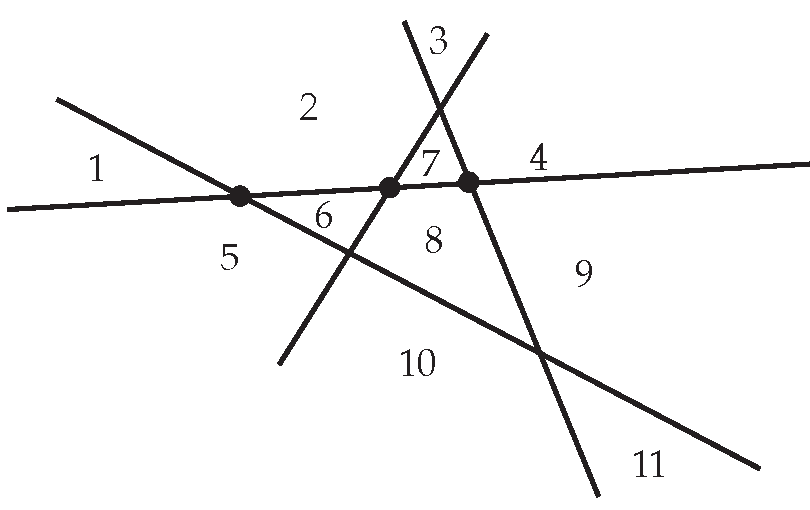
\includegraphics[width=0.5\textwidth]{induction-figs/lines-regions}
    \caption{Lines and regions in the plane}
    \label{fig:induction:lines-regions}
  \end{figure}
  With the recursive formula, we thus have $r(5)=5+11=16$,
  $r(6)=6+16=22$ and $r(7)=7+22=29$. Even by hand, it wouldn't be all
  that much trouble to calculate $r(100)$.  We could do it before
  lunch.

\end{example}

\begin{example}
  A $2\times n$ checkerboard will be tiled with rectangles of size
  $2\times1$ and $1\times2$.  Find a recursive formula for the number
  $t(n)$ of tilings.  Clearly, $t(1)=1$ and $t(2)=2$.  When $n>2$,
  consider the rectangle that covers the square in the upper right
  corner.  If it is vertical, then preceding it, we have a tiling of
  the first $n-1$ columns.  If it is horizontal, then so is the
  rectangle immediately underneath it, and proceeding them is a tiling
  of the first $n-2$ columns.  This shows that $t(n)=t(n-1)+t(n-2)$.
  In particular, $t(3)=1+2=3$, $t(4)=2+3=5$ and $t(5)= 3+5=8$.
\end{example}

Again, if compelled, we could get $t(100)$ by hand, and a computer
algebra system could get $t(1000)$.

\begin{example}
  Call a ternary string \textit{good} if it never contains a $2$
  followed immediately by a $0$; otherwise, call it \textit{bad}. Let
  $g(n)$ be the number of good strings of length $n$. Obviously
  $g(1)=3$, since all strings of length $1$ are good.  Also, $g(2)=8$
  since the only bad string of length~$2$ is $(2,0)$.  Now consider a
  value of $n$ larger than~$2$.

  Partition the set of good strings of length~$n$ into three parts,
  according to the last character. Good strings ending in $1$ can be
  preceded by any good string of length $n-1$, so there are $g(n-1)$
  such strings. The same applies for good strings ending in $2$. For
  good strings ending in $0$, however, we have to be more careful. We
  can precede the $0$ by a good string of length~$n-1$ provided that
  the string does not end in $2$. There are $g(n-1)$ good strings of
  length~$n-1$ and of these, exactly $g(n-2)$ end in a~$2$.  Therefore
  there are $g(n-1)-g(n-2)$ good strings of length~$n$ that end in
  a~$0$.  Hence the total number of good strings of length~$n$
  satisfies the recursive formula $g(n) = 3g(n-1) - g(n-2)$.  Thus
  $g(3) = 3\cdot8 -3= 21$ and $g(4)= 3\cdot21-8= 55$.
\end{example}

Once more, $g(100)$ is doable by hand, while even a modest computer can be
coaxed into giving us $g(5000)$.

\subsection{Finding Greatest Common Divisors}\label{s:induction:gcd}

There is more meat than you might think to the following elementary
theorem, which seems to simply state a fact that you've known since
second grade.

\begin{theorem}[Division Theorem]\label{thm:division}
Let $m$ and $n$ be positive integers.  Then there exist
unique integers $q$ and $r$ so that
\[
m = q\cdot n+r\quad\text{and}\quad 0 \le r < n.
\]
We call $q$ the \emph{quotient} and $r$ the \emph{remainder}.
\end{theorem}

\begin{proof} 
We settle the claim for existence.  The uniqueness part is
just high-school algebra.  If the theorem fails to hold, then
let $t$ be the least positive integer for which there are
integers $m$ and $n$ with $m+n=t$, but there
do not exist integers $q$ and $r$ with $m=qn+r$ and $0\le r<n$.

First, we note that $n\neq 1$, for if $n=1$, then we could take
$q=m$ and $r=0$.  Also, we cannot have $m=1$, for if $m=1$, then
we can take $q=0$ and $r=1$.  Now the statement holds for the
pair $m-1$, $n$ so there are integers $q$ and $r$ so that

\[
m-1 = q\cdot n+r\quad\text{and}\quad 0 \le r < n.
\]
Since $r<n$, we know that $r+1\le n$.  If $r+1<n$, then
\[
m = q\cdot n+(r+1)\quad\text{and}\quad 0 \le r+1 < n.
\]
On the other hand, if $r+1=n$, then
\[
m = q\cdot n+(r+1)=nq+n=(q+1)n=(q+1)n+0.
\]
The contradiction completes the proof.
\end{proof}

Recall that an integer $n$ is a \emph{divisor} of an integer $m$ if
there is an integer $q$ such that $m=qn$. (We write $n\mid m$ and read
``$n$ divides $m$''.) An integer $d$ is a \emph{common divisor} of
integers $m$ and $n$ if $d$ is a divisor of both $m$ and $n$. The
\emph{greatest common divisor} of $m$ and $n$, written $\gcd(m,n)$, is
the largest of all the common divisors of $m$ and $n$.

Here's a particularly elegant application of the preceding basic
theorem:

\begin{theorem}[Euclidean Algorithm]\label{thm:euclideanalg}
Let $m,n$ be positive integers and let $q$ and $r$ be
the unique integers for which
\[
m = q\cdot n+r\quad\text{and}\quad 0 \le r < n.
\]
If $r>0$, then $\gcd(m,n)=\gcd(n,r)$.
\end{theorem}
\begin{proof}
  Consider the expression $m=q\cdot n+r$, which is equivalent to
  $m-q\cdot n = r$. If a number $d$ is a divisor
  of $m$ and $n$, then $d$ must also divide $r$.  Similarly, if $d$ is
  a divisor of $n$ and $r$, then $d$ must also divide $m$.
\end{proof}

Here is a code snippet that computes the greatest common divisor of
$m$ and $n$ when $m$ and $n$ are positive integers with $m\ge n$.  We
use the familiar notation $m\%n$ to denote the remainder $r$ in the
expression $m=q\cdot n+r$, with $0\le r < n$.

\medskip
\begin{tt}
\noindent
int gcd(int m, int n) \{\\
\hspace{.25in}\mbox{} if (m\%n == 0) return n;\\
\hspace{.25in}\mbox{} else return gcd(n, m\%n);\\
\}\\
\end{tt}

\medskip The disadvantage of this approach is the somewhat wasteful
use of memory due to recursive function calls. It is not difficult to
develop code for computing the greatest common divisor of $m$ and $n$
using only a loop, i.e., there are no recursive calls. With minimal
extra work, such code can also be designed to solve the following
diophantine equation problem:

\begin{theorem}\label{thm:gcd-dioph}
  Let $m$, $n$, and $c$ be positive integers.  Then there exist
  integers $a$ and $b$, not necessarily non-negative, so that
  $am+bn=c$ if and only if $c$ is a multiple of the greatest common
  divisor of $m$ and $n$.
\end{theorem}

Let's see how the Euclidean algorithm can be used to write $\gcd(m,n)$
in the form $am+bn$ with $a,b\in\ints$ with the following example.

\begin{example}
  Find the greatest common divisor $d$ of $3920$ and $252$ and find
  integers $a$ and $b$ such that $d=3920a+252b$.

  In solving the problem, we demonstrate how to perform the Euclidean
  algorithm so that we can find $a$ and $b$ by working
  backward. First, we note that
  \[3920 = 15\cdot 252 + 140.\]
  Now the Euclidean algorithm tells us that
  $\gcd(3920,252)=\gcd(252,140)$, so we write
  \[252 = 1\cdot 140 + 112.\]
  Continuing, we have $140= 1\cdot 112 + 28$ and $112 = 4\cdot 28+0$,
  so $d=28$. 

  To find $a$ and $b$, we now work backward through the equations we
  found earlier, ``solving'' them for the remainder term and then
  substituting. We begin with
  \[28 = 140-1\cdot 112.\]
  But we know that $112=252-1\cdot 140$, so
  \[28=140-1(252-1\cdot 140) = 2\cdot 140 - 1\cdot 252.\]
  Finally, $140 = 3920-15\cdot 252$, so now we have
  \[28= 2(3920-15\cdot 252) - 1\cdot 252 = 2\cdot 3920-31\cdot 252.\]
  Therefore $a=2$ and $b=-31$.
\end{example}

\subsection{Sorting}

One of the most common and most basic computing problems is sorting:
Given a sequence $a_1,a_2,\dots,a_n$ of $n$ distinct integers,
rearrange them so that they are in increasing order.  We describe
here an easy recursive strategry for accomplishing this task.  This
strategy is known as \textit{Merge Sort}, and it is one of several
optimal algorithms for sorting.  Introductory computer science
courses treat this topic in greater depth.  In our course, we simply
need some good strategy and merge sort works fine for our purposes.

To present merge sort, must first develop a strategy for solving a 
special case of the sorting problem.
Suppose we have two $s+t$ distinct integers
$\{u_1,u_2,\dots,u_s,v_1,v_2,\dots,v_t\}$ with $u_1<u_2<\dots<u_s$
and $v_1<v_2<\dots<v_t$.  How do we \textit{merge} these two sequences
into a single increasing sequence of length $s+t$.
Imagine the two sequences placed on two horizontal lines, one immediately
under the other.  Then let $u$ be the least integer in the first
sequence and $v$ the least integer in the second.  At the moment,
this implies that $u=u_1$ and $v=v_1$, but integers will be deleted 
from the two sequences as the process is carried out.  Regardless, the 
meaning of $u$ and $v$ will be preserved.   Also, set $n=1$.
Then take $a_n$ as the minimum of $u$ and $v$ and delete $a_n$ from
the sequence in which it occurs.  Then increase $n$ by $1$ and
repeat.  Here is a code snippet for accomplishing a merge operation,
with $u_p$ now written as $u[p]$.  

\medskip
\begin{tt}
\noindent
p = q = 1;
for (i = 1; i < s+t+1; i++) \{\\
a[i] = min(u[p], v[q]);\\
if (min(u[p], v[q])==u[p]) p = p+1;\\
\quad  else q = q+1;\\
\}\\
\end{tt}

Now that we have a good strategy for merging, it is easy to
develop a recursive strategy for sorting.  Given a sequence
$a_1,a_2,\dots,a_n$ of $n$ distinct integers, we set $s=\lceil n/2\rceil$
and $t=\lfloor n/2\rfloor$.  Then let $u_i=a_i$ for $i=1,2,\dots,s$ and
$v_j=a_{s+j}$, for $j=1,2,\dots,t$.  Sort the two subsequences
and then merge them.  For a concrete example, given the
sequence $(2,8,5,9,3,7,4,1,6)$, we split into $(2,8,5,9,3)$ and
$(7,4,1,6)$.  These subsequences are sorted (by a recursive call)
into $(2,3,5,8,9)$ and $(1,4,6,7)$, and then these two sorted
sequences are merged.

For running time, if $S(n)$ is the number of operations it takes
to sort a sequence of $n$ distinct integers, then $S(2n)\le2 S(n) + 2n$,
since it clearly takes $2n$ steps to merge two sorted sequences
of length $n$.  This leads to the bound  $S(n) = O(n\log n)$,
and in computer science courses, you will learn (here it is an
exercise) that this is optimal.

\section{Mathematical Induction}\label{s:induction:induction}

Now we move on to induction, the powerful twin of recursion.

Let $n$ be a positive integer. Consider the following mathematical 
statements, each of which involve $n$:

\begin{enumerate}
\item $2n+7 = 13$.
\item $3n-5=9$.
\item $n^2-5n+9=3$.
\item $8n-3 < 48$.
\item $8n-3 > 0$.
\item $(n+3)(n+2) =n^2+5n+6$.
\item $n^2 -6n + 13 \ge 0$.
\end{enumerate}

Such statements are called \textit{open} statements.  Open statements
can be considered as \textit{equations}, i.e., statements that are
valid for certain values of $n$.  Statement~1 is valid only when
$n=3$.  Statement~2 is never valid, i.e., it has no solutions among
the positive integers. Statement~3 has exactly two solutions, and
Statement~4 has six solutions.  On the other hand, Statements~5, 6
and~7 are valid for all positive integers.

At this point, you are probably scratching your head, thinking that
this discussion is trivial.  But let's consider some statements that
are a bit more complex.

\begin{enumerate}
\item The sum of the first $n$ positive integers is $n(n+1)/2$.
\item The sum of the first $n$ odd positive integers is $n^2$.
\item $n^n \ge  n! + 4,000,000,000n2^n$\quad when $n\ge 14$.
\end{enumerate}

How can we establish the validity of such statements, provided of
course that they are actually true?  The starting point for providing
an answer is the following property:

\medskip 
\noindent\textbf{Principle of Mathematical Induction} Let $S_n$ be an open
statement involving a positive integer $n$.  If $S_1$ is true, and if
for each positive integer $k$, assuming that the statement $S_k$ is
true implies that the statement $S_{k+1}$ is true, then $S_n$ is true
for every positive integer~$n$.

\medskip With a little thought, you should see that the Principle of
Mathematical Induction is logically equivalent to the Well Ordered
Property of Positive Integers.  If you haven't already done so, now
might be a good time to look over \autoref{app:background} on background
material.
 
\section{Inductive Definitions}\label{s:induction:inductdefs}

Although it is primarily a matter of taste, recursive
definitions can also be recast in an inductive setting.
As a first example, set $1!=1$ and whenever $k!$ has
been defined, set $(k+1)!=(k+1)k!$.

As a second example, set
\[
\sum_{i=1}^1 f(i) = f(1)\quad\text{and}\quad
 \sum_{i=1}^{k+1} f(i)= \sum_{i=1}^{k} f(i)+ f(k+1) 
\]
In this second example, we are already using an abbreviated
form, as we have omitted some English phrases. 
But the meaning should be clear.

Now let's back up and give an example which would really
be part of the development of number systems.  Suppose
you knew everything there was to know about the \textit{addition}
of positive integers but had never heard anything about
\textit{multiplication}.  Here's how this operation can
be defined. 

Let $m$ be a positive integer.  Then set
\[
m\cdot1 = m\quad\text{and}\quad m\cdot(k+1)=m\cdot k+ m
\]
You should see that this \textit{defines} multiplication
but doesn't do anything in terms of establishing such
familiar properties as the commutative and associative
properties.  Check out some of the details in \autoref{app:background}. 

\section{Proofs by Induction}\label{s:induction:proofs}

No discussion of recursion and induction would be
complete without some obligatory examples of proofs using
induction.  We start with the ``Hello World'' example. 

\begin{proposition}\label{prop:sumints}
  For every positive integer $n$, the sum of the first $n$ positive
  integers is $n(n+1)/2$, i.e.,
\[
\sum_{i=1}^n i=\frac{n(n+1)}{2}.
\]
\end{proposition}

For our first version of a proof of
\hyperref[prop:sumints]{Proposition~\ref*{prop:sumints}}, we clearly
identify the open statement $S_n$ and describe the proof carefully in
terms of $S_n$. As you develop more experience with writing proofs by
induction, this will become less essential, as you'll see in the
second version of the proof.

\begin{proof}[First proof]
  Let $n$ be a positive integer, and let $S_n$ be the open statement 
  \[\sum_{i=1}^n i = \frac{n(n+1)}{2}.\]
  We will prove that $S_n$ is true for all positive integers by
  induction. For the basis step, we must prove that $S_1$ is
  true. When $n=1$, the left-hand side of $S_n$ is just $1$, while the
  right-hand side evaluates to $1(1+1)/2=1$. Therefore, $S_1$ is true.

  Next we assume that for some positive integer $k$, $S_k$ is
  true. That is, we assume 
  \[
  \sum_{i=1}^k i=\frac{k(k+1)}{2}.
  \]
  We now seek to prove that $S_{k+1}$ is true, and begin by
  considering the left-hand side of $S_{k+1}$. We notice that
  \[
  \sum_{i=1}^{k+1}i=\left(\sum_{i=1}^k i\right) +(k+1)=
  \frac{k(k+1)}{2}+(k+1),\]
  since our inductive hypothesis that $S_k$ is true gives us the
  simpler formula for the summation. Now continuing with a bit of
  algebra, we find
  \[\frac{k(k+1)}{2}+(k+1)=\frac{k^2+3k+2}{2}=\frac{(k+1)(k+2)}{2}.
  \]
  Therefore, $S_{k+1}$ is true.  Since we have shown that $S_1$ is
  true and that for every positive integer $k$, if $S_k$ is true,
  then $S_{k+1}$ is true, we conclude that $S_n$ is true for all
  positive integers $n$ by the Principle of
  Mathematical Induction.
\end{proof}

Before looking at a refined version of this proof, let's take a moment
to discuss the key steps in every proof by induction. The first step
is the \emph{basis step}, in which the open statement $S_1$ is shown to be
true. (It's worth noting that there's nothing special about $1$
here. If we want to prove only that $S_n$ is true for all integers
$n\geq 5$, then proving that $S_5$ is true is our basis step.) When
proving the basis step, if $S_n$ is an equation, we do not just write
down $S_1$ and move on. We need to \emph{prove} that $S_1$ is
true. Notice how in the proof above, we discussed the left-hand side
of $S_1$ and the right-hand side of $S_1$ and concluded that they were
equal.

After the basis step comes the \emph{inductive step}, in which we
assume that $S_k$ is true for \textbf{some} positive integer $k$ and
prove that $S_{k+1}$ is true. When doing this, we call $S_k$ our
\emph{inductive hypothesis}. In the inductive step, the most common
mistake students make is starting with the entirety of $S_{k+1}$ and
manipulating it until they obtain a true statement. This is dangerous,
as it is possible to start with something false and through valid
algebraic steps, obtain a true statement. Instead, the best option is
to work as with the basis step: if $S_{k+1}$ is an equation or inequality,
work on one side until you find a place to apply the inductive
hypothesis and then continue until you obtain the other side. If the
algebra gets tricky along the way, you can also work with the
left-hand side of $S_{k+1}$ and separately work with the right-hand side of
$S_{k+1}$. If you're able to manipulate both sides to be in the same
form, then you have shown they are equal and $S_{k+1}$ is true.

Now let's take a look at a more refined proof of
\hyperref[prop:sumints]{Proposition~\ref*{prop:sumints}}. From here
on, when we give a proof by induction, we'll use this style. As you're
getting started with induction proofs, you may find it useful to be
more explicit about the steps as we did in the first proof above.

\begin{proof}[Refined proof]
  We first prove the assertion when $n=1$.  For this value of $n$, the
  left-hand side is just~$1$, while the right-hand side evaluates to
  $1(1+1)/2=1$.

  Now assume that for some positive integer $k$, the formula holds
  when $n=k$, i.e., assume that
  \[
  \sum_{i=1}^k i=\frac{k(k+1)}{2}.
  \]
  Then it follows that
  \[
  \sum_{i=1}^{k+1}i=\left(\sum_{i=1}^k i\right) +(k+1)=
  \frac{k(k+1)}{2}+(k+1)=\frac{k^2+3k+2}{2}=\frac{(k+1)(k+2)}{2}.
  \]
  Thus the formula also holds when $n=k+1$.  By the Principle of
  Mathematical Induction, it holds for all positive integers $n$.
\end{proof}

The preceding arguments are 100\% correct\dots but some combinatorial
mathematicians would argue that they may actually hide what is really
going on.  These folks would much prefer a combinatorial proof, as was
provided in the preceding chapter.  Our perspective is that you should
prefer to give a combinatorial proof---when you can find one.  But if
pressed, you should be able to give a formal proof by mathematical
induction.

Here's a second example, also quite a classic.  Again, recall that we
gave a combinatorial proof in the last chapter. As you read the proof,
make sure you can identify the open statement $S_n$, the basis step,
and the inductive step.

\begin{proposition}\label{prop:sumodd}
For each positive integer $n$, the
sum of the first $n$ odd positive integers is $n^2$, i.e.,
\[
\sum_{i=1}^n (2i-1)= n^2.
\]
\end{proposition}
\begin{proof}
We will prove this by induction. First, note that the formula holds when
$n=1$.  Now suppose that $k$ is a positive integer and
that the formula holds when $n=k$, i.e., assume
\[
\sum_{i=1}^k (2i-1)= k^2.
\]
Then
\[
\sum_{i=1}^{k+1}(2i-1)=\left(\sum_{i=1}^k 2i-1\right)+2k+1=
k^2+(2k+1)=(k+1)^2.
\]
Therefore, the proposition follows by the Principle of Mathematical Induction.
\end{proof}

Here's a more general version of the first result in
this section, and again we note that we gave a combinatorial
proof in the last chapter.

\begin{proposition}\label{prop:sum-bincoeffs}
Let $n$ and $k$ be non-negative integers with $n\ge k$.
Then
\[
\sum_{i=k}^n \binom{i}{k}=\binom{n+1}{k+1}.
\]
\end{proposition}
\begin{proof}
Fix a non-negative integer $k$.  We then prove the
formula by induction on $n$.  If $n=k$, note that
the left hand side is just $\binom{k}{k}=1$, while the
right hand side is $\binom{k+1}{k+1}$ which is also~$1$.
Now assume that $m$ is a non-negative integer, with 
$m\ge k$, and that the
formula holds when $n=m$, i.e., assume that
\[
\sum_{i=k}^m \binom{i}{k}=\binom{m+1}{k+1}.
\]

Then
\begin{align*}
\sum_{i=k}^{m+1}\binom{i}{k} &= \sum_{i=k}^{m}\binom{i}{k} +\binom{m+1}{k}\\
        &=\binom{m+1}{k+1}+\binom{m+1}{k}\\
        &=\binom{m+2}{k+1}.
\end{align*} 
Therefore, the proposition follows by the Principle of Mathematical Induction.
\end{proof}


\section{Strong Induction}\label{s:induction:strong-induction}

There are occasions where the Principle of Induction, at least
as we have studied it up to this point, does not seem sufficient.
Here is a concrete example.
The professor asked Bob to study a function  $f(n)$ defined recursively by
$f(n) = 2f(n-1) - f(n-2)$ with $f(1)=3$ and $f(2)=5$.  Specifically,
the professor asked Bob to compute $f(10^{10})$, which seems like 
a daunting task.  Over coffee, Bob scribbled on a napkin and determined
that $f(3)=7$ and $f(4)=9$, and on the basis of these calculations alone,
he thought that it might just be possible that  
$f(n) = 2n+1$ for all $n\geq 1$.  If this were true, he could
simply report that $f(10^{10})=2\cdot 10^{10}+1=20000000001$.

Bob was beginning to understand proofs by induction, so he tried to
prove that $f(n)=2n+1$ for all $n\ge1$ by induction. For the base step,
he noted that $f(1)= 3=2\cdot1+1$, so all is ok to this point.
For the inductive step, he assumed that $f(k)=2k+1$ for some $k\ge1$
and then tried to prove that $f(k+1)=2(k+1)+1$.  If this step could be completed,
then the proof by induction would be done.

But at this point, Bob seemed to hit a barrier, because 
\[f(k+1) = 2f(k) - f(k-1) = 2(2k+1) - f(k-1),
\]
using the inductive hypothesis to replace $f(k)$ by $2k+1$. However,
he's was totally perplexed about what to do with the $f(k-1)$.  If he knew
that $f(k-1)=2(k-1)+1$, then the right hand side
would result in $2(2k+1) -(2k-1)= 2k+3=2(k+1)+1$, which is
exactly what he wants.  Bob always plays by the rules, and he
has to admit that he doesn't know that $f(k-1)=2(k-1)+1$.  He
only knows that $f(k)=2k+1$.

Bob was about to throw in the towel and ask his computer to start
making the calculations recursively, when
Carlos comes along and asks what he's doing. Carlos sees right away
that the approach Bob was taking to prove that $f(n)=2n+1$ by induction
won't work---but after a moment's reflection, Carlos says that there's
a stronger form of an inductive proof that will do the trick.
Carlos patiently explained to Bob a proposition which is called the
\textit{Strong} Principle of Mathematical Induction.  To prove that
an open statement $S_n$ is valid for all $n\ge1$, it is enough to
(a)~Show that $S_1$ is valid, and (b)~Show that $S_{k+1}$ is valid
whenever $S_m$ is valid for all integers $m$ with $1\le m\le k$.

The validity of this proposition is trivial since it is \textit{stronger}
than the principle of induction.  What is novel here is that in order
to prove a statement, it is sometimes to your advantage to prove
something even stronger.  Combinatorial mathematicians call this
the ``bootstrap'' phenomenon.

Equipped with this observation, Bob saw clearly that the strong principle
of induction was enough to prove that $f(n)=2n+1$ for all $n\ge1$.
So he could power down his computer and enjoy his coffee.

\section{Discussion}\label{s:induction:discussion}
 
The group was debating the value of combinatorial proofs versus
formal proofs by induction.  Xing said that he actually preferred to
do a proof by induction, as a combinatorial proof, it could be
argued, wasn't really a proof.  Dave mumbled ``Combinatorial proofs
can always be made rigorous.''   They went back and forth for a
while and then Alice said ``But the professor never explained
that weird sequence

\[
1,2,3,4,1,2,3,4,5,1,2,3,4,5,2,3,4,5,6,2,3,4,5,6,1,2,3,4,5,2,3,4,5,6,\dots
\]
Dave was on a roll ``Who has change for a dollar?'' but nobody
understood why he would derail an argument over proofs when
everybody had already paid for the coffee.  Alice was more to the
point ``You know Dave, sometimes I just don't understand why
you say  the things you do.''  Dave smiled (maybe it was more of
a smirk) ``It's about making change.  The terms in this sequence
are the fewest number of coins required to make change.''
Bob said ``I don't get it.'' Dave continued ``The term  $a_n$ is
the fewest number of U.S. coins required to total to $n$ cents.''
Now everyone groaned, everyone except Carlos, who thought that
at least this time, Dave was really clever.

``Well'', said Bob ``that takes care of the strange sequence,
but I still don't see any difference between
induction and recursion.  Dave couldn't keep quiet ``No one does.''  Xing thought
differently and said ``In many programming languages, you try to
avoid recursion, preferring to use loops instead.  Otherwise, you
wind up overloading the stack.  As just one example, you can
compute the greatest common divisor $d$ of $m$ and $n$, as well as
find $a$ and $b$ so that $d=am+bn$ using a loop---with very
little storage.  The recursive approach discussed previously, with 
the inherent back tracking at the end, isn't really necessary.''  
Yolanda was impressed with Xing's extensive programming experience and 
knowledge, but Alice was less so.  

Zori was losing her patience and was especially grumpy today ``I don't
see any value to any of this stuff.  Who's going to pay me to find
greatest common divisors?''  Dave said ``Nobody.''  Alice said ``But
maybe there are some principles here that have practical application.''
Carlos joined in ``I think the basic principles behind establishing
that a computer program does what you intend have a lot to do with
induction and recursion.''  Bob said ``I don't understand.  When
I write a program, I just pay attention to details and after just 
a few corrections, they always work.''  Alice was brutal ``Maybe that's
because you don't do anything complicated.''  Carlos was more gentle
``Big software projects might have hundreds of thousands of lines
of code, and pieces of the final product might be written by
different groups of programmers at different moments in time.
Establishing correctness can be a very difficult task.''
Zori's ears perked up as she thought she saw something in
this last bit of conversation that might be a way to earn a salary.

\section{Exercises}\label{s:induction:exercises}

For questions asking you find a recursive formula, be sure to give
enough initial values to get the recursion going.


\begin{enumerate}\item  A database uses record identifiers that are alphanumeric
    strings in which the $10$ decimal digits and $26$ upper-case
    letters are valid symbols. The criteria that define a valid record
    identifier are recursive. A valid record identifier of length
    $n\geq 2$ can be constructed in the following ways:
    \begin{itemize}
    \item beginning with any upper-case letter other than $D$ and
      followed by any valid record identifier of length $n-1$;
    \item beginning with $1C$, $2K$, or $7J$ and followed by any valid
      record identifier of length $n-2$; or
    \item beginning with $D$ and followed by any string of $n-1$
      decimal digits.
    \end{itemize}
    Let $r(n)$ denote the number of valid record identifiers of length
    $n$. We take $r(0)=1$ and note that $r(1) = 26$. Find a recursion
    for $r(n)$ when $n\geq 2$ and use it to compute $r(5)$.
\item    Consider a $1\times n$ checkerboard. The squares of the
    checkerboard are to be painted white and gold, but no two
    consecutive squares may both be painted white. Let $p(n)$ denote
    the number of ways to to paint the checkerboard subject to this
    rule. Find a recursive formula for $p(n)$ valid for $n\geq 3$.
\item   Give a recursion for the number $g(n)$ of ternary strings of
    length $n$ that do not contain $102$ as a substring.

\item A $2\times n$ checkerboard is to be tiled using two types of
  tiles. The first tile is a $1\times 1$ square tile. The second tile
  is called an $L$-tile and is formed by removing the upper-right
  $1\times 1$ square from a $2\times 2$ tile. The $L$-tiles can be
  used in any of the four ways they can be rotated. (That is, the
  ``missing square'' can be in any of four positions.) Let $t(n)$
  denote the number of tilings of the $2\times n$ checkerboard using
  $1\times 1$ tiles and $L$-tiles. Find a recursive formula for $t(n)$ and
  use it to determine $t(7)$.
\item Let $S$ be the set of strings on the alphabet $\{0,1,2,3\}$ that
  do not contain $12$ or $20$ as a substring. Give a recursion for the
  number $h(n)$ of strings in $S$ of length $n$. \textit{Hint}: Check
  your recursion by manually computing $h(1)$, $h(2)$, $h(3)$, and
  $h(4)$.
  %Solution: $h(n)=4h(n-1)-2h(n-2)+h(n-3)$ with $h(1)=4$,
  %  $h(2)=14$, and $h(3)=49$ and h(4) = 172

\item Find $d=\gcd(5544,910)$ as well as integers $a$ and $b$ such
  that $5544a + 910 b = d$.
\item Find $\gcd(827,249)$ as well as integers $a$ and $b$ such that
  $827a+249b = 6$.
\item Let $a$, $b$, $m$, and $n$ be integers and suppose that
  $am+bn=36$. What can you say about $\gcd(m,n)$?
\item  (A challenging problem)  For
  each formula, give both a proof using the Principle of
  Mathematical Induction and a combinatorial proof. One of the two
  will be easier while the other will be more challenging.
  \begin{enumerate}
  \item $\displaystyle 1^2+2^2+3^2+\dots+ n^2= \frac{n(n+1)(2n+1)}{6}$
%  \item $\displaystyle\binom{n}{0}\binom{n}{n}+\binom{n}{1}\binom{n}{n-1}+
%    \binom{n}{2}\binom{n}{n-2}+\dots+\binom{n}{n}\binom{n}{0}=\binom{2n}{n}$
  \item $\displaystyle\binom{n}{0}2^0+\binom{n}{1}2^1+\binom{n}{2}2^2+\dots+\binom{n}{n}2^n=3^n$
  \end{enumerate}
\item Show that for all integers $n\geq 4$, $2^n < n!$.
\item Show that for all positive integers $n$,
  \[\sum_{i=0}^n 2^i = 2^{n+1}-1.\]
\item Show that for all positive integers $n$, $7^n-4^n$ is divisible
  by $3$.
\item Show that for all positive integers $n$, $9^n-5^n$ is divisible
  by $4$.
\item It turns out that if $a$ and $b$ are positive integers with
  $a>b+1$, then there is a positive integer $M>1$ such that $a^n-b^n$
  is divisible by $M$ for all positive integers $n$. Determine $M$ in
  terms of $a$ and $b$ and prove that it is a divisor of $a^n-b^n$ for
  all positive integers $n$.
\item Use mathematical induction to prove that for all integers $n\geq
  1$,
  \[n^3 + (n+1)^3 + (n+2)^3\]
  is divisible by $9$.
\item Give a proof by induction of the Binomial Theorem
  (\autoref{thm:binomial}). How do you think it compares to the
  combinatorial argument given in \autoref{ch:strings}?
\item Consider the recursion given by $f(n) = 2f(n-1) - f(n-2) + 6$
  for $n\geq 2$ with $f(0)=2$ and $f(1)=4$. Use mathematical induction
  to prove that $f(n) = 3n^2-n+2$ for all integers $n\geq 0$.
\item Consider the recursion given by $f(n) = f(n-1)+f(n-2)$ for
  $n\geq 3$ with $f(1)=f(2)=1$. Show that $f(n)$ is divisible by $3$
  if and only if $n$ is divisible by $4$.
\item Suppose that $x\in\reals$ and $x>-1$. Prove that for all
  integers $n\geq 0$, $(1+x)^n\geq 1+nx$.
\item Show that there is a positive constant $c$ so that any algorithm 
 that sorts a sequence of $n$ positive integers must, in worst case, take 
 $cn\log n$ steps. \emph{Hint}:  There are $n!$ permutations of a set of $n$
 distinct integers.  Each operation reduces the number of possibilities
 by a multiplicative fraction which is at most $1/2$.  So if there
 are $t$ operations, then $2^t\ge n!$.  Now look up Stirling's
 approximation for $n!$ and continue from there.
\end{enumerate}

%%% Local Variables: 
%%% mode: latex
%%% TeX-master: "chap-skel-mtk"
%%% End: 

% basics.tex
% Updated January 11, 2012

\chapter{Combinatorial Basics}\label{ch:basics}

Dave hates doing the same thing twice.  He sees himself
as a free spirit and never wants to fall into a rut.  Alice
says that this approach to life requires one to have lots
and lots of options, for if you have to do a lot of something,
like get up in the morning and get dressed, then you may not
be able to avoid mindless repetition, dull and boring as it
may seem.

\section{The Pigeon Hole Principle}\label{s:basics:pigeonhole}

A function $f:X\longrightarrow Y$ is said to be $1$--$1$ when
$f(x)\neq f(x')$ for all $x,x'\in X$ with $x\neq x'$.  A $1$--$1$
function is also called an \textit{injection}.  When
$f:X\longrightarrow Y$ is $1$--$1$, we note that $|X|\le |Y|$.
Conversely, we have the following self-evident statement, which is
popularly called the ``Pigeon Hole'' principle.

\begin{proposition}\label{prop:pigeon}
If $f:X\longrightarrow Y$ is a function and $|X|>|Y|$, then
there exists an element $y\in Y$ and distinct elements $x,x'\in X$
so that $f(x)=f(x')=y$.
\end{proposition}

In more casual language, if you must put $n+1$ pigeons into $n$ holes,
then you must put two pigeons into the same hole.

Here is a classic result, whose proof follows immediately from
the Pigeon Hole principle.

\begin{theorem}[Erd\H{o}s/Szekeres]\label{thm:ErdosSzekeres}
If $m$ and $n$ are non-negative integers, then 
any sequence of $mn+1$ distinct real numbers 
either has an increasing subsequence of $m+1$ terms, or it has a 
decreasing subsequence of $n+1$ terms.
\end{theorem}
\begin{proof}
Let $\sigma=(x_1,x_2,x_3,\dots,x_{mn+1})$ be a sequence of
$mn+1$ distinct real numbers.  For each $i=1,2,\dots,mn+1$, let $a_i$ be the
maximum number of terms in a increasing subsequence of
$\sigma$ with $x_i$ the first term.  Also, let $b_i$ be the maximum number
of terms in a decreasing subsequence of $\sigma$ with $x_i$
the last term.  If there is some $i$ for which $a_i\ge m+1$, then
$\sigma$ has an increasing subsequence of $m+1$ terms.  Conversely, if
for some $i$, we have $b_i\ge n+1$, then we conclude that $\sigma$ has
a decreasing subsequence of $n+1$ terms.

It remains to consider the case where $a_i\le m$ and $b_i\le n$ for all
$i=1,2,\dots,mn+1$.  Since there are $mn$ ordered pairs of the form
$(a,b)$ where $1\le a\le m$ and $1\le b\le n$, we conclude from the
Pigeon Hole principle that there must be integers $i_1$ and $i_2$ with
$1\le i_1<i_2\le mn+1$ for which $(a_{i_1},b_{i_1})=(a_{i_2},b_{i_2})$.
Since $x_{i_1}$ and $x_{i_2}$ are distinct, we either have $x_{i_1}<x_{i_2}$
or $x_{i_1}>x_{i_2}$.  In the first case, any increasing subsequence of 
with $x_{i_2}$ as its first term can be extended by prepending
$x_{i_1}$ at the start.  This shows that $a_{i_1}>a_{i_2}$.  
In the second case, any decreasing sequence of with $x_{i_1}$ as its last 
element can be extended by adding $x_{i_2}$ at the very end.  This
shows $b_{i_2}>b_{i_1}$.
\end{proof}

In \autoref{ch:probmeth}, we will explore some powerful
generalizations of the Pigeon Hole principle.  All these results have
the flavor of the general assertion that total disarray is impossible.

\section{An Introduction to Complexity Theory}\label{s:basics:complexity}

\begin{discussion}
Bob says that he's really getting to like this combinatorial
mathematics stuff. The concrete nature of the subject is appealing.
But he's not sure that he understands the algorithmic component.
Sometimes he sees how one might actually compute the answer to a
problem---provided he had access to a powerful computer.  At other
times, it seems that a computational approach might be out of
reach, even with the world's best and fastest computers at ready
access.  Carlos says it can be much worse than that.  There are
easily stateable problems that no one knows how to attack even
if all the world's computational power is used in concert.  And there's nothing on the
horizon that will change that.  In fact, build faster computers and
you just change the threshold for what is computable.  There will still
be easily understood problems that will remain unresolved.
\end{discussion}

\subsection{Three Questions}\label{s:basics:questions}

We consider three problems with a common starting point.  You are
given\footnote{The particulars of how the set is given to you
aren't important to the discussion.  For example, the data could be given
as a text file, with one number on each line.} a set $S$ of 
$10,000$ distinct positive integers, each at most
$100,000$,  and then asked the following questions.

\begin{enumerate}
\item Is $83,172$ one of the integers in the set $S$?
\item Are there three integers in $S$ whose sum is $143,297$?
\item Can the set $S$ be partitioned as $S=A\cup B$ with
$A\cap B=\emptyset$, so that $\sum_{a\in A}a=\sum_{b\in B}b$.
\end{enumerate}

The first of the three problems sounds easy, and it is.  You just consider
the numbers in the set one by one and test to see if any of them is
$83,172$.  You can stop if you ever find this number and
report that the answer is yes.  If you return a no answer, then you
will have to have read every number in the list.  Either way, you halt
with a correct answer to the question having done at most $10,000$
tests, and even the most modest netbook can do this in a heartbeat.
And if the list is expanded to $1,000,000$ integers, all at most
a billion, you can still do it easily.  More generally, if you're
given a set $S$ of $n$ numbers and an integer $x$ with the question
``Is $x$ a member of $S$?'', you can answer this question in
$n$ steps, with each step an operation of testing a number in $S$
to see if it is exactly equal to $n$.  So the running time of this
algorithm is proportional to $n$, with the constant depending on
the amount of time it takes a computer to perform the basic operation
of asking whether a particular integer is equal to the target value.

The second of the three problems is a bit more challenging.  Now it seems
that we must consider the $3$-element subsets of a set of size $10,000$.
There are $C(10,000,3)$ such sets.  On the one hand, testing three
numbers to see if their sum is $143,297$ is very easy, but there are lots
and lots of sets to test.  Note that $C(10,000,3)=166,616,670,000$, and not
too many computers will handle this many operations.  Moreover, if the
list is expanded to a million numbers, then we have more than $10^{17}$
triples to test, and that's off the table with today's hardware.

Nevertheless, we can consider the general case.  We are given a set $S$ of $n$
integers and a number $x$.  Then we are asked whether there are
three integers in $S$ whose sum is $x$.  The algorithm we have
described would have running time proportional to $n^3$, where the constant
of proportionality depends on the time it takes to test a triple of
numbers to see if there sum is $x$.  Of course, this depends in turn
on just how large the integer $x$ and the integers in $S$ can be.

The third of the three problems is different. First, it seems to be much harder.
There are $2^{n-1}$ complementary pairs of subsets of a set of size~$n$,
and one of these involves the emptyset and the entire set.  But that
leaves $2^{n-1}-1$ pairs to test.  Each of these tests is not all that
tough.  A netbook can easily report whether a two subsets have the
same sum, even when the two sets form a partition of a set of size
$10,000$, but there are approximately $10^{3000}$ partitions to test
and no piece of hardware on the planet will touch that assignment.
And if we go up to a set of size $1,000,000$, then the combined computing
power of all the machines on earth won't get the job done.

In this setting, we have an algorithm, namely testing all partitions,
but it is totally unworkable for $n$ element sets when $n$ is large since 
it has running time proportional to $2^n$.

\subsection{Certificates}

Each of the three problems we have posed is in the form of a
``yes/no'' question. A ``yes'' answer to any of the three can be justified
by providing a certificate.  For example, if you answer the first
question with a yes, then you might provide the additional information
that you will find $83,172$ as the integer on line $584$ in the input
file.  Of course, you could also provide the source code for the
computer program, and let a referee run the entire procedure.

Similarly, if you answer the second question with a yes,
then you could specify the three numbers and specify where in
the input file they are located.  An impartial referee could then
verify, if it mattered, that the sum of the three integers was
really $143,297$ and that they were located at the specified places
in the input file.  Alternatively, you could again provide the source
code which would require the referee to test all triples and
verify that there is one that works.

Likewise, a yes for the third question admits a modest size
certificate.  You need only specify the elements of the subset $A$.
The referee, who is equipped with a computer, can (a)~check to see that
all numbers in $A$ belong to $S$; (b)~form a list of the subset $B$ consisting
of those integers in $S$ that do not belong to $A$; and (c)~compute
the sums of the integers in $A$ and the integers in $B$ and verify that
the two sums are equal.  But in this case, you would not provide 
source code for the algorithm, as there does not appear (at least nothing
in our discussion thus far provides one) to be a reasonable strategy
for deciding this problem when the problem size is large.

Now let's consider the situation with a ``no'' answer.  When the answer
to the first question is no, the certificate can again be a computer program
that will enable the referee to consider all the elements of $S$ and
be satisfied that the number in question is not present.  A similar
remark holds for the second question, i.e., the program is the certificate.

But the situation with the third question is again very different.
Now we can't say to the referee ``We checked all the possibilities and
none of them worked.''  This could not possibly be a true statement.
And we have no computer program that can be run by us or by the 
referee.  The best we could say is that we tried to find a suitable partition 
and were unable to do so. As a result, we don't know what the correct answer 
to the question actually is.

\subsection{Operations}

Many of the algorithms we develop in this book, as well as many of
the computer programs that result from these algorithms involve
basic steps that are called \textit{operations}.  The meaning of
the word operation is intentionally left as an imprecise notion.
An operation might be just comparing two integers to see if they
are equal; it might be updating the value of a variable $x$ and
replacing it by $x^2-3x+7$; and it might be checking whether two
set sums are equal.  In the third instance, we would typically
limit the size of the two subsets as well as the integers in them.
As a comsequence, we want to be able to say that there is some
constant $c$ so that an operation can be carried out in time
at most $c$ on a computer. Different computers yield different
values of $c$, but that is a discrepancy which we can safely ignore.

\subsection{Input Size}

Problems come in various sizes.  The three problems we have discussed
in this chapter have the same input size.   Roughly speaking this
size is $10,000$ blocks, with each block able to hold an integer
of size at most $100,000$.  In this text, we will say that the
input size of this problem is $n=10,000$, and in some sense ignoring
the question of the size of the integers in the set.  There are 
obvious limitations to this approach.  We could be given a set $S$
of size~$1$ and a candidate element $x$ and be asked whether $x$ belongs
to $S$.  Now suppose that $x$ is a bit string the size of a typical
compact disk, i.e., some $700$ megabytes in length.  Just reading the single
entry in $S$ to see if it's exactly $x$ will take some time.

In a similar vein, consider the problem of determing whether a file
$x$ is located anywhere in the directory structure under $y$ in
a unix file system.  If you go on the basis of name only, then
this may be relatively easy.  But what if you want to be sure that an exact copy
of $x$ is present.  Now it is much more challenging.

\section{The Big ``Oh'' and Little ``Oh'' Notations}\label{s:basics:big-oh}

Let $f:\mathbb{N}\longrightarrow \mathbb{R}$ and
$g:\mathbb{N}\longrightarrow\mathbb{R}$ be functions.
We write $f=O(g)$, and say $f$ is ``Big Oh'' of $g$,  
when there is a constant $c$ and an integer
$n_0$ so that $f(n)\le cg(n)$ whenever $n>n_0$.
Although this notation has a long history, we can provide
a quite modern justification.  If $f$ and $g$ both describe
the number of operations  required for two algorithms given input
size $n$, then the meaning of $f=O(g)$ is that $f$ is no
harder than $g$ when the problem size is large.

We are particulary interested in comparing functions against
certain natural benchmarks, e.g.,  $\log\log n$, $\log n$, $\sqrt{n}$, 
$n^\alpha$ where $\alpha<1$,  $n$, $n^2$, $n^3$, $n^c$ where $c>1$ 
is a constant, $n^{\log n}$, $2^n$, $n!$, $2^{n^2}$, etc.

For example, later in this text, we will learn that there
are sorting algorithms with running time $O(n\log n)$ where
$n$ is the number of integers to be sorted.  As a second 
example, we will learn that we can find all shortest paths in 
an oriented graph on $n$ vertices with non-negative weights on edges with an 
algorithm having running time $O(n^2)$.  At the other extreme,
no one knows whether there is a constant $c$ and an algorithm for 
determining whether the chromatic number of a graph is at most three
which has running time $O(n^c)$.  

It is important to remember that when we write $f=O(g)$, we are
implying in some sense that $f$ is no bigger than $g$, but it
may in fact be much smaller.  By contrast, there will be times
when we really know that one function dominates
another.  And we have a second kind of notation to capture this
relationship.

Let $f:\mathbb{N}\longrightarrow \mathbb{R}$ and
$g:\mathbb{N}\longrightarrow\mathbb{R}$ be functions with
$f(n)>0$ and $g(n)>0$ for all $n$.  We write $f=o(g)$, and 
say that $f$ is ``Little oh'' of $g$, when 
$\lim_{n\rightarrow\infty}f(n)/g(n)=0$. 
For example $\ln n=o(n^{.2})$; $n^\alpha=o(n^{\beta})$ whenever
$0<\alpha<\beta$; and $n^{100}=o(c^n)$ for every $c>1$.
In particular, we write $f(n)=o(1)$ when $\lim_{n\rightarrow\infty}f(n)=0$.

\section{Exact Versus Approximate}\label{s:basics:exact}

Many combinatorial problems admit ``exact'' solutions, and in these
cases, we will usually try hard to find them.  The Erd\H{o}s/Szekeres
theorem from earlier in this chapter is a good example of an
``exact'' result\footnote{Exact results are also called ``best possible'', ``sharp'' 
or ``tight.''}.  By this statement,
we mean that for each pair $m$ and $n$ of positive integers, there
is a sequence of $mn$ distinct real numbers that has neither
an increasing subsequence of size $m+1$ nor a decreasing subsequence
of size~$n+1$.  To see this, consider the sequence $\sigma$ defined
as follows: For each $i=1,2,\dots,m$,
let $B_i=\{j+(m-1)i:1\le j\le n\}$.  Note that each $B_i$ is a block
of $n$ consecutive integers.  Then define a permutation $\sigma$ of
the first $mn$ integers by setting $\alpha<\beta$ if there exist
distinct integers $i_1$ and $i_2$ so that $\alpha\in B_{i_1}$ and
$\beta\in B_{i_2}$.  Also, for each $i=1,2,\dots,m$, set $\alpha<\beta$
in $\sigma$ when $1+(m-1)i\le \beta<\alpha\le n+(m-1)i$.  Clearly,
any increasing subsequence of $\sigma$ contains at most one member
from each block, so $\sigma$ has no increasing sequence of size~$m=1$.
On the other hand, any decreasing sequence in $\sigma$ is contained
in a single block, so $\sigma$ has no decreasing sequence of size $n+1$.

As another example of an exact solution, the number of integer solutions 
to $x_1+x_2+\dots x_r=n$ with $x_i>0$ for $i-1,2,\dots,r$ is exactly $C(n-1,r-1)$.
On the other hand, nothing we have discussed thus far allows us to provide
an exact solution for the number of partitions of an integer~$n$.

\subsection{Approximate and Assymptotic Solutions}

Here's an example of a famous problem that we can only discuss in terms of
approximate solutions, at least when the input size is suitably large.
For an integer $n$, let $\pi(n)$ denote the number of primes among the 
first $n$ positive integers.  For example, 
$\pi(12)=5$ since $2$, $3$, $5$, $7$ and $11$ are primes.   
The exact value of $\pi(n)$ is known when $n\le 10^{23}$, and in fact: 
\[
\pi(10^{23}) = 1,925,320,391,606,803,968,923
\]
On the other hand, you might ask whether $\pi(n)$ tends to infinity
as $n$ grows larger and larger.  The answer is yes, 
and here's a simple and quite classic argument.  Suppose
to the contrary that there were only $k$ primes, where $k$ is a positive
integer.  Suppose these $k$ primes are listed in increasing order as
$p_1<p_2<\dots<p_k$, and consider the number $n=1+p_1p_2\cdots p_k$.
Then $n$ is not divisible by any of these primes, and it is larger than
$p_k$, which implies that $n$ is a prime number larger than $p_k$.

So we know that $\lim_{n\rightarrow\infty}\pi(n)=\infty$.
In a situation like this, mathematicians typically want to know more about 
how fast $\pi(n)$ goes to infinity.  Some functions go to infinity ``slowly'',
such as $\log n$ or $\log\log n$.  Some go to infinity quickly, like
$2^n$, $n!$ or $2^{2^n}$.  Since $\pi(n)\le n$, it can't go to infinity
as fast as these last three functions, but it might go infinity like
$\log n$ or maybe $\sqrt{n}$. 

On the basis of computational results (done by hand, long before there
were computers), Legendre conjectured in 1796 that $\pi(n)$ goes to
infinity like $n/\ln n$.  To be  more precise, he conjectured that
\[
\lim_{n\rightarrow\infty}\frac{\pi(n)\ln n}{n}=1.
\]
In 1896, exactly one hundred years after Legendre's conjecture, 
Hadamard and de la Vall\'ee-Poussin independently published proofs
of the conjecture, using techniques whose roots are in the
Riemann's pioneering work in complex analysis.  This result, now
known simply as the \textit{Prime Number Theorem}, continues to this
day to be much studied topic at the boundary of analysis and number
theory.

\subsection{Polynomial Time Algorithms}

Throughout this text, we will place considerable emphasis on
problems which admit polynomial time solutions.  This refers
to problems for which there is some constant $c>0$ so that there
is an algorithm $\cgA$ for solving the problem which has running
time $O(n^c)$ where $n$ is the input size.
the symbol $\cgP$ is suggestive of \textit{polynomial}.


\subsection{$\mathcal{P}=\mathcal{NP}$?}

Perhaps the most famous question at the boundary of
combinatorial mathematics, theoretical computer science
and mathematical logic is the notoriously challenging
question of deciding whether $\mathcal{P}$ is the same
as $\mathcal{NP}$.  This problem has the shorthand form:
$\mathcal{P}=\mathcal{NP}$?  Here, we present
a brief informal discussion of this problem.

First, we have already introduced the class $\cgP$ consisting of all 
yes-no combinatorial problems which admit polynomial time algorithms.
The first two problems discussed in this chapter belong to
$\cgP$ since they can be solved with algorithms that
have running time $O(n)$ and $O(n^3)$, respectively.
Also, determing whether a graph is $2$-colorable and whether it
is connected both admit polynomial time algorithms.  

We should emphasize that it may be very difficult to determine
whether a problem belongs to class $\mathcal{P}$ or not.
For example, we don't see how to give a fast algorithm for
solving the third problem (subset sum), but that doesn't mean
that there isn't one.  Maybe we all need to study harder!

Setting that issue aside for the moment, the class $\mathcal{NP}$ consists of
yes--no problems for which there is a certificate for
a yes answer whose correctness can be verified in polynomial
time. More formally, this is called the class of \textit{nondeterministic
polynomial time} problems.  Our third problem definitely belongs to this class.

So the famous question is to detemine whether the two
classes are the same.  Evidently, any problem belonging
to $\cgP$ also belongs to $\mathcal{NP}$, i.e,
$\cgP\subseteq\mathcal{NP}$, but are they equal?
It seems difficult to believe that there is a polynomial
time algorithm for settling the third problem (the subset
sum problem), and no one has come close to settling this
issue.  But if you get a good idea, be sure to discuss it with
one or both authors of this text before you go public with
your news.  If it turns out that you are right, you are
certain to treasure a photo opportunity with yours truly.

\section{Discussion}\label{s:basics:discussion}

Carlos, Dave and Yolanda were fascinated by the discussion on complexity.
Zori was less enthusiastic but even 
she sensed that the question of which problems could be solved quickly
had practical implications. She could even predict that people could
earn a nice income solving problems faster and more accurately
than their competition.

Bob remarked ``I'm not sure I understand what's being talked about
here.  I don't see why it can't be the  case that all problems
can be solved.  Maybe we just don't know how to do it.''
Xing said ``Any finite problem \textit{can} be solved.  There
is always a way to list all the possibilities, compare them
one by one and take the best one as the answer.''
Alice joined in ``Well, a problem might take a long time
just because it is big.  For example, suppose you are given
two dvd's, each completely full with the data for a large integer.
How are you possibly going to multiply them together, even
with a large computer and fancy software.''  Carlos then
offered ``But I think there are really hard problems that
any algorithm will take a long time to solve and not just
because the input size is large.  At this point, I don't know how 
to formulate such a problem but I suspect that they exist.''

\section{Exercises}\label{s:basics:exercises}

\begin{enumerate}
\item  Suppose you are given a list of $n$ integers, each of size
at most $100n$.   How many operations would it take you to do the following
tasks (in answering these questions, we are interested primarily in whether it
will take $\log n$, $\sqrt{n}$, $n$, $n^2$, $n^3$, $2^n$, \dots steps.  In 
other words, ignore multiplicative constants.):

\begin{enumerate} 
\item Determine if the number $2n+7$ is in the list.
\item Determine if there are two numbers in the list whose sum is
$2n+7$.
\item Determine if there are two numbers in the list whose product is
$2n+7$ (This one is more subtle than it might appear!  It may be
to your advantage to sort the integers in the list).
\item Determine if there is a number $i$ for which all the numbers in
the list are between $i$ and $i+2n+7$. 
\item Determine  the longest sequence of consecutive integers belonging
to the list.
\item Determine the number of primes in the list. 
\item Determine whether there are three integers $x$, $y$ and $z$ from
the list so that $x+y=z$.
\item Determine whether there are three integers $x$, $y$ and $z$ from
the list so that $x^2+y^2=z^2$.
\item Determine whether there are three integers $x$, $y$ and $z$ from
the list so that $xy=z$.
\item Determine whether there are three integers $x$, $y$ and $z$ from
the list so that $x^y=z$.
\item Determine whether there are two integers $x$ and $y$ from
the list so that $x^y$ is a prime.
\item Determine the longest arithmetic progression in the list (a
sequence $(a_1, a_2,\dots,a_t)$ is an arithmetic progression when
there is a constant $d\neq 0$ so that $a_{i+1}=a_i+d$, for each $i=1,2,
\dots, t-1$).
\item Determine the number of distinct sums that can be formed from
members of the list (arbitrarily many integers from the list are allowed to
be terms in the sum).
\item Determine the number of distinct products that can be formed from
members of the list (arbitrarily many integers from the list are allowed to be
factors in the product).
\item Determine for which integers $m$, the list contains at least $10\%$ of the
integers from $\{1,2,\dots,m\}$.

\end{enumerate}

\item If you have to put $n+1$ pigeons into $n$ holes, you have to
put two pigeons into the same hole.  What happens if you have to
put $mn+1$ pigeons into $n$ holes?

\item Consider the set $X=\{1,2,3,4,5\}$ and suppose you have two holes.
Also suppose that you have $10$ pigeons: the $2$-element subsets of
$X$.  Can you put these $10$ pigeons into the two holes in a way that there
is no $3$-element subset $S=\{a,b,c\}\subset X$ for which all pigeons from
$S$ go in the same hole?  Then answer the same question if $X=\{1,2,3,4,5,6\}$
with $15 = C(6,2)$ pigeons.

\item  Let $n=10,000$. Suppose a friend tells you that he has a secret family of subsets
of $\{1,2,\dots,n\}$, and if you guess it correctly, he will give you one million
dollars.  You think you know the subset he has in mind and it contains exactly
half the subsets, i.e., the family has $2^{n-1}$ subsets.  Discuss how you can
share your hunch with your friend in an effort to win the prize.   

\item  Let $N$ denote the set of positive integers.  When $f:N\rightarrow N$ is
a function, let $E(f)$ be the function defined by $E(f)(n) = 2^{f(n)}$.
What is $E^5(n^2)$?

\end{enumerate}
%%% Local Variables: 
%%% mode: latex
%%% TeX-master: "book"
%%% End: 

% graphs.tex
% Updated January 11, 2012

\chapter{Graph Theory}\label{ch:graphs}

In \hyperref[ex:radiostations]{Example~\ref*{ex:radiostations}}, we
discussed the problem of assigning frequencies to radio stations in
the situation where stations within $200$ miles of each other must
broadcast on distinct frequencies. Clearly we would like to use the
smallest number of frequencies possible for a given layouts of
transmitters, but how can we determine what that number is?

Suppose three new homes are being built and each of them must be
provided with utility connections. The utilites in question are water,
electricity, and natural gas. Each provider needs a direct line from
their terminal to each house (the line can zig-zag all it wants, but
it must go from the terminal to the house without passing through
another provider's terminal or another house en route), and the three
providers all wish to bury their lines exactly four feet below
ground. Can they do this successfully without the lines crossing?

These are just two of many, many examples where the discrete structure
known as a \emph{graph} can serve as an enlightening mathematical
model. Graphs are perhaps the most basic and widely studied
combinatorial structure, and they are prominently featured in this
text. Many of the concepts we will study, while presented in a more
abstract mathematical sense, have their origins in applications of
graphs as models for real-world problems.

\section{Basic Notation and Terminology for Graphs}\label{s:graphs:intro}

A \textit{graph} $\bfG$ is a pair $(V,E)$ where $V$ is a set (almost
always finite) and $E$ is a set of $2$-element subsets of $V$.
Elements of $V$ are called \textit{vertices} and elements of $E$ are
called \textit{edges}.  We call $V$ the \textit{vertex set} of $\bfG$
and $E$ is the \textit{edge set}.  For convenience, it is customary to
abbreviate the edge $\{x,y\}$ as just $xy$.  Remember though that
$xy\in E$ means exactly the same as $yx\in E$.  If $x$ and $y$ are
distinct vertices from $V$, $x$ and $y$ are \textit{adjacent} when
$xy\in E$; otherwise, we say they are \textit{non-adjacent}. We say
the edge $xy$ is \emph{incident to} the vertices $x$ and $y$.

For example, we could define a graph $\GVE$ with vertex set
$V=\{a,b,c,d,e\}$ and edge set $E=\{\{a,b\},\{c,d\},\{a,d\}\}$. Notice
that no edge is incident to $e$, which is perfectly permissible based
on our definition. It is quite common to identify a graph with a
visualization in which we draw a point for each vertex and a line
connecting two vertices if they are adjacent. The graph $\bfG$ we've
just defined is shown in \autoref{fig:small_graph}. It's important to
remember that while a drawing of a graph is a helpful too, it is not
the same as the graph. We could draw $\bfG$ in any of several
different ways without changing what it is as a graph.

\begin{figure}[h]
  \centering
  \begin{overpic}{graphs-figs/small_graph}
    \put(58,100){$a$}
    \put(100,48){$b$}
    \put(-7,10){$c$}
    \put(15,50,){$d$}
    \put(70,11){$e$}
  \end{overpic}
  \caption{A graph on $5$ vertices}
  \label{fig:small_graph}
\end{figure}

As is often the case in science and mathematics, different authors use
slightly different notation and terminology for graphs.  As an
example, some use \textit{nodes} and \textit{arcs} rather than
vertices and edges.  Others refer to vertices as \textit{points} and
in this case, they often refer to \textit{lines} rather than edges.
We will try to stick to vertices and edges but confess that we may
occasionally lapse into referring to vertices as points.  Also,
following the patterns of many others, we will also say that adjacent
vertices are \textit{neighbors}.  And we will use the more or less
standard terminology that the \textit{neighborhood} of a vertex $x$ is
the set of vertices adjacent to $x$. Thus, using the graph $\bfG$ we
have depicted in \autoref{fig:small_graph}, vertices $d$ and $a$ are
neighbors, and the neighborhood of $d$ is $\{a,c\}$ while the
neighborhood of $e$ is the empty set. Also, the \textit{degree} of a
vertex $v$ in a graph $\bfG$, denoted $\deg_\bfG(v)$, is then the
number of vertices in its neighborhood, or equivalently, the number of
edges incident to it. For example, we have
$\deg_\bfG(d)=\deg_\bfG(a)=2$, $\deg_\bfG(c)=\deg_\bfG(b)=1$, and
$\deg_\bfG(e)=0$. If the graph being discussed is clear from context,
it is not uncommon to omit the subscript and simply write $\deg(v)$
for the degree of $v$.

When $\GVE$ and $\HWF$ are graphs, we say $\bfH$ is a
\textit{subgraph} of $\bfG$ when $W\subseteq V$ and $F\subseteq E$.
We say $\bfH$ is an \textit{induced} subgraph when $W\subseteq V$ and
$F=\{xy\in E: x,y\in W\}$. In other words, an induced subgraph is
defined completely by its vertex set and the original graph $\bfG$. We
say $\bfH$ is a \textit{spanning} subgraph when $W=V$. In
\autoref{fig:subgraphs}, we show a graph, a subgraph and an induced
subgraph. Neither of these subgraphs is a spanning subgraph.

\begin{figure}
\begin{center}
\includegraphics*[width=4in]{graphs-figs/subgraphs}
\caption{\label{fig:subgraphs}A Graph, a Subgraph and an Induced Subgraph}
\end{center}
\end{figure}

A graph $\GVE$ is called a \textit{complete} graph when $xy$ is an
edge in $\bfG$ for every distinct pair $x,y\in V$.  Conversely, $\bfG$
is an \textit{independent} graph if $xy\not\in E$, for every distinct
pair $x,y\in V$.  It is customary to denote a complete graph on $n$
vertices by $\bfK_n$ and an independent graph on $n$ vertices by
$\bfI_n$. In \autoref{fig:complete_graphs}, we show the complete
graphs with at most $5$ vertices.

\begin{figure}
  \centering
  \begin{overpic}[width=4in]{graphs-figs/complete_graphs}
    \put(2.5,2){$\bfK_1$}
    \put(16.5,2){$\bfK_2$}
    \put(36.5,2){$\bfK_3$}
    \put(60.5,2){$\bfK_4$}
    \put(86,2){$\bfK_5$}
  \end{overpic}
  \caption{Small complete graphs}
  \label{fig:complete_graphs}
\end{figure}

A sequence $(x_1,x_2,\dots,x_n)$ of vertices in a graph $\GVE$ is
called a \textit{walk} when $x_ix_{i+1}$ is an edge for each
$i=1,2,\dots,n-1$.  Note that the vertices in a walk need not be
distinct.  On the other hand, if the vertices are distinct, then the
sequence is called a \textit{path}, and often to emphasize where a
path starts and ends, we will say that a sequence
$(x_1,x_2,\dots,x_n)$ of distinct vertices is a path from $x_1$ to
$x_n$ in $\bfG$. Similarly, when $n\ge3$, a path $(x_1,x_2,\dots,x_n)$
of $n$ distinct vertices is called a cycle when $x_1x_n$ is also an
edge in $\bfG$.  It is customary to denote a path on $n$ vertices by
$\bfP_n$, while $\bfC_n$ denotes a cycle on $n$ vertices. The
\emph{length} of a path or a cycle is the number of edges it
contains. Therefore, the length of $\bfP_n$ is $n-1$ and the length of
$\bfC_n$ is $n$. In \autoref{fig:paths}, we show the paths of length
at most $4$, and in \autoref{fig:cycles}, we show the cycles of length
at most $5$.

\begin{figure}
  \centering
  \begin{overpic}[width=4in]{graphs-figs/paths}
    \put(8,-2){$\bfP_1$}
    \put(24,-2){$\bfP_2$}
    \put(39.5,-2){$\bfP_3$}
    \put(59.5,-2){$\bfP_4$}
    \put(85,-2){$\bfP_5$}
  \end{overpic}
  \caption{Short paths}
  \label{fig:paths}
\end{figure}
\begin{figure}
  \centering
  \begin{overpic}[width=4in]{graphs-figs/cycles}
    \put(24,1){$\bfC_3$}
    \put(47.5,1){$\bfC_4$}
    \put(73,1){$\bfC_5$}
  \end{overpic}
  \caption{Small cycles}
  \label{fig:cycles}
\end{figure}


If $\GVE$ and $\HWF$ are graphs, we say $\bfG$ is \textit{isomorphic}
to $\bfH$ and write $\bfG\cong\bfH$ when there exists a bijection
$f:V\bijection W$ so that $x$ is adjacent to $y$ in $\bfG$ if and only
if $f(x)$ is adjacent to $f(y)$ in $\bfH$.  Often writers will say
that $\bfG$ ``contains'' $\bfH$ when there is a subgraph of $\bfG$
which is isomorphic to $\bfH$.  In particular, it is customary to say
that $\bfG$ contains the cycle $\bfC_n$ (same for $\bfP_n$ and
$\bfK_n$) when $\bfG$ contains a subgraph isomorphic to $\bfC_n$. The
graphs in \autoref{fig:isomorphic} are isomorphic. An isomorphism
between these graphs is given by
\[f(a)=5,\quad f(b) = 3, \quad f(c) = 1,\quad f(d) = 6,\quad f(e)=2,\quad f(h)=4.\]
\begin{figure}
  \centering
  \begin{overpic}[width=4in]{graphs-figs/isomorphic_graphs}
    \put(6,13){$a$}
    \put(20.5,1){$b$}
    \put(36,14){$c$}
    \put(20,21){$d$}
    \put(38,2){$e$}
    \put(22.5,13){$h$}

    \put(83,13.5){$1$}
    \put(67,10){$2$}
    \put(85,2){$3$}
    \put(67.5,21.5){$4$}
    \put(53,13){$5$}
    \put(68,1){$6$}
  \end{overpic}
  \caption{A pair of isomorphic graphs}
  \label{fig:isomorphic}
\end{figure}
On the other hand, the graphs shown in \autoref{fig:nonisomorphic} are
\emph{not} isomorphic, even though they have the same number of
vertices and the same number of edges. Can you tell why?
\begin{figure}
  \centering
  \begin{overpic}[width=4in]{graphs-figs/nonisomorphic_graphs}
    \put(6,13){$a$}
    \put(20.5,1){$b$}
    \put(36,14){$c$}
    \put(20,21){$d$}
    \put(38,2){$e$}
    \put(22.5,13){$h$}

    \put(83,13.5){$1$}
    \put(73.2,10){$2$}
    \put(85,2){$3$}
    \put(67.5,21.5){$4$}
    \put(53,13){$5$}
    \put(68,1){$6$}
  \end{overpic}
  \caption{A pair of nonisomorphic graphs}
  \label{fig:nonisomorphic}
\end{figure}


 A graph $\bfG$ is \textit{connected} when there is
a path from $x$ to $y$ in $\bfG$, for every $x,y\in V$; otherwise, we
say $\bfG$ is \textit{disconnected}. The graph of
\autoref{fig:small_graph} is disconnected (a sufficient justification
for this is that there is no path from $e$ to $c$), while those in
\autoref{fig:isomorphic} are connected.

A graph is \textit{acyclic} when it does not contain any cycle on
three or more vertices.  Acyclic graphs are also called
\textit{forests}.  A connected acyclic graph is called a
\textit{tree}.  When $\GVE$ is a connected graph, a subgraph $\HWF$ of
$\bfG$ is called a \textit{spanning tree} if $\bfH$ is both a spanning
subgraph of $\bfG$ and a tree. In \autoref{fig:spantree}, we show a
graph and one of its spanning trees. We will return to the subject of
spanning trees in \autoref{ch:graphalgorithms}.
\begin{figure}
\begin{center}
\includegraphics*[width=4in]{graphs-figs/spanning_tree}
\caption{\label{fig:spantree}A Graph and a Spanning Tree}
\end{center}
\end{figure}

The following theorem is very elementary, and some authors refer to it
as the ``first theorem of graph theory''. However, this basic result
can be surprisingly useful.

\begin{theorem}
  Let $\deg_\bfG(v)$ denote the degree of vertex $v$ in graph $\GVE$. Then
  \[\sum_{v\in V}\deg_\bfG(v) = 2|E|.\eqno{(*)}\]
\end{theorem}

\begin{proof}
  We consider how many times an edge $e=vw\in E$ contributes to each
  side of (*). The $\deg_\bfG(x)$ and $\deg_\bfG(y)$ terms on the left
  hand side each count $e$ once, so $e$ is counted twice on that
  side. On the right hand side, $e$ is clearly counted
  twice. Therefore, we have the equality claimed.
\end{proof}

\begin{corollary}
  For any graph, the number of vertices of odd degree is even.
\end{corollary}

We will return to the topic of trees later, but before moving on, let
us prove one elementary proposition about trees. First, a
\textit{leaf} in a tree $\bfT$ is a vertex $v$ with $\deg_\bfT(v)=1$.

\begin{proposition}\label{prop:tree-leaves}
  Every tree on $n\geq 2$ vertices has at least two leaves.
\end{proposition}

\begin{proof}
  Our proof is by induction on $n$. For $n=2$, there is precisely one
  tree, which is isomorphic to $\bfK_2$. Both vertices in this graph
  are leaves, so the proposition holds for $n=2$. Now suppose that for
  some integer $m\geq 2$, every tree on at most $m$ vertices has at
  least two leaves and let $\bfT=(V,E)$ be a tree on $m+1$ vertices.
  Pick an edge $e\in E$ and form a new graph $\bfT'=(V',E')$ by
  deleting $e$ from $\bfT$. That is, $V'=V$ and $E'=E-\{e\}$. Now
  since $\bfT'$ does not contain a path from one endpoint of $e$ to
  its other endpoint, $\bfT'$ is not connected. However, deleting an
  edge cannot create a cycle, so $\bfT'$ is a forest. Furthermore, it
  has precisely two components, each of which is a tree with at most
  $m$ vertices. If each component has at least two vertices, then by
  induction, each has at least two leaves. In the worst case scenario,
  two of these leaves are the endpoints of $e$, so at least two of the
  vertices are leaves in $\bfT$, too. If each component of $\bfT'$ has
  only one vertex, then $\bfT\cong \bfK_2$, which has two leaves. If
  exactly one of the components has only one vertex, then it must be a
  leaf in $\bfT$. Thus, applying the inductive hypothesis to the other
  component ensures that there is a second leaf in $\bfT$.
 % First note that $\bfT$ must have a leaf, as if all vertices had
  % degree at least $2$, you could start at a vertex $v$ and walk from
  % $v$ to another vertex $v'$ and from $v'$ to another vertex and so on
  % but would eventually double back on the vertices you'd already
  % visited, since any time you visit a vertex for the first time there
  % is a way to exit the vertex to another vertex. This would create a
  % cycle, contrary to the fact that $\bfT$ is a tree. Let $v_0$ be the
  % leaf that we know must exist and let $\bfT'$ be the subgraph of
  % $\bfT$ induced by all the vertices \emph{except} $v_0$. Then $\bfT'$
  % is also a tree (removing $v_0$ cannot create a disconnected graph)
  % and has $m$ vertices, so by induction $\bfT'$ has at least two
  % leaves, $v_1$ and $v_2$. At least one of $v_1$ and $v_2$ is also a
  % leaf in $\bfT$, since $v_0$ can be adjacent to at most one of them,
  % and therefore $\bfT$ has at least two leaves.
\end{proof}

\section{Multigraphs:  Loops and Multiple Edges}\label{s:graphs:multigraphs}

Consider a graph in which the vertices represent cities and the edges
represent highways.  Certain pairs of cities are joined by an edge
while other pairs are not.  The graph may or may not be connected
(although a disconnected graph is likely to result in disgruntled
commuters).  However, certain aspects of real highway networks are not
captured by this model. First, between two nearby cities, there can
actually be several interconnecting highways, and traveling on one
of them is fundamentally different from traveling on another.  This
leads to the concept of \textit{multiple edges}, i.e., allowing for
more than one edge between two adjacent vertices.  Also, we could have
a highway which leaves a city, goes through the nearby countryside and
the returns to the same city where it originated.  This leads to the
concept of a \textit{loop}, i.e., an edge with both end points being
the same vertex.  Also, we can allow for more than one loop with the
same end point.

Accordingly, authors frequently lead off a discussion on a graph
theory topic with a sentence or two like:
\begin{enumerate}
\item In this paper, all graphs will be \textit{simple}, i.e., we will
  not allow loops or multiple edges.
\item In this paper, graphs can have loops and multiple edges.
\end{enumerate}
The terminology is far from standard, but in this text, a graph will
always be a \textit{simple} graph, i.e., no loops or multiple edges.
When we want to allow for loops and multiple edges, we will use the
term \textit{multigraph}.  This begs the question of what we would
call a graph if it is allowed to have loops but not multiple edges, or
if multiple edges are allowed but not loops.  If we \textit{really}
needed to talk about such graphs, then the English language comes to
our rescue, and we just state the restriction explicitly!

\section{Eulerian and Hamiltonian Graphs}\label{s:graphs:eulerham}

Graph theory is an area of mathematics that has found many
applications in a variety of disciplines. Throughout this text, we
will encounter a number of them. However, graph theory traces its
origins to a problem in K\"onigsberg, Prussia (now Kaliningrad,
Russia) nearly three centuries ago. The river Pregel passes through
the city, and there are two large islands in the middle of the
channel. These islands were connected to the mainland by seven bridges
as indicated in \autoref{fig:bridges}. It is said that the citizens of
K\"onigsberg often wondered if it was possible for one to leave his
home, walk through the city in such a way that he crossed each bridge
precisely one time, and end up at home again. Leonhard Euler settled
this problem in 1736 by using graph theory in the form of
\autoref{thm:eulerian}.

\begin{figure}
  \centering
  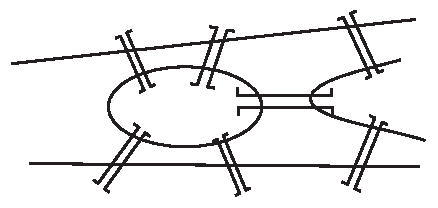
\includegraphics{graphs-figs/konigsberg_bridges}
  \caption{\label{fig:bridges}The bridges of K\"onigsberg}
\end{figure}

A graph $\bfG$ is \textit{eulerian} if there is a sequence
$(x_0,x_1,x_2,\dots,x_t)$ of vertices from $\bfG$, with repetition
allowed, so that
\begin{enumerate}
\label{def:eulerian-circuit}
\item $x_0=x_t$;
\item for every $i=0,1,\dots t-1$, $x_ix_{i+1}$ is an edge of $\bfG$;
\item for every edge $e\in E$, there is a unique
  integer $i$ with $0\le i<t$ for which $e=x_ix_{i+1}$.
\end{enumerate}
When $\bfG$ is eulerian, a sequence satisfying these three conditions
is called an \textit{eulerian circuit}. A sequence of vertices
$(x_0,x_1,\dots,x_t)$ is called a \textit{circuit} when it satisfies
only the first two of these conditions.  Note that a sequence
consisting of a single vertex is a circuit. The following elementary
theorem completely characterizes eulerian graphs.  It comes with an
algorithmic proof, one that is easily implemented.

\begin{theorem}\label{thm:eulerian}
  A graph $\bfG$ is eulerian if and only if it is connected and 
  every vertex has even degree.
\end{theorem}

\begin{proof}
  Clearly, an eulerian graph must be connected.  Also, if $(x_0,x_1,\dots,x_t)$
  is an eulerian circuit in $\bfG$, then for each $i=0,1,\dots,t-1$,
  we can view the edge $x_ix_{i+1}$ as exiting $x_i$ and entering $x_{i+1}$.
  The degree of every vertex must be even, since for each vertex $x$, the
  number of edges exiting $x$ equals the number of edges entering $x$.
  Furthermore, each edge incident with $x$ either exits from $x$ or enters~$x$.

  We now describe a deterministic process that will either (a)~find
  an eulerian circuit, (b) show that the graph is disconnected, or
  (c)~find a vertex of odd degree.
  The description is simplified by assuming that the vertices in
  $\bfG$ have been labelled with the positive integers $1,2,\dots,n$, where
  $n$ is the number of vertices in $\bfG$.  Furthermore, we take $x_0=1$.

  We launch our algorithm with a trivial circuit $C$ consisting of
  just the vertex $x_0=(1)$.  Thereafter suppose that we have a partial
  circuit $C$ defined by a sequence $(x_0, x_1,\dots,x_t)$ with
  $x_0=x_t=1$. The edges
  of the form $x_ix_{i+1}$ have been \textit{traversed}, while the
  remaining edges in $\bfG$ (if any) have not.  If the third condition
  for an euler circuit is satisfied, we are done, so we assume it does
  not hold.

  We then choose the least integer $i$ for which there is an edge
  incident with $x_i$ that has not already been traversed.  If there
  is no such integer, since there are edges that have not yet been
  traversed, then we have discovered that the graph is disconnected.
  So we may assume that the integer $i$ exists.  Set $u_0=x_i$.  We
  define a sequence $(u_0,u_1,\dots,u_s)$ recursively.  If $j\ge 0$, set
  \[
   N_j=\{y: u_jy\text{ is an edge in $\bfG$ and has not yet been traversed.}\}
 \] 
  If  $N_j\neq\emptyset$, we take $u_{j+1}$ as the least positive integer
  in $N_j$. If $N_j=\emptyset$, then $j\ge1$ and we take $s=j$ and halt
  this subroutine.
  
  When the subroutine halts, we consider two cases.  If $u_0\neq u_s$,
  then $u_0$ and $u_s$ are vertices of odd degree in  $\bfG$.  So we
  are left to consider the case where $u_0=u_s=x_i$.  In this case,
  we simply expand our original sequence $(x_0,x_1,\dots,x_t)$ by
  replacing the integer $x_i$ by the sequence $(u_0,u_1,\dots,u_s)$.
\end{proof}

As an example, consider the graph $\bfG$ shown in \autoref{fig:graphs:eulerexample}.
Evidently, this graph is connected and all vertices have even degree.
Here is the sequence of circuits starting with the trivial circuit $C$
consisting only of the vertex~$1$.
\begin{align*}
C &=(1)\\
  &=(1,2,4,3,1)\quad \text{start next from $2$}\\ 
  &=(1,2,5,8,2,4,3,1)\quad\text{start next from $4$}\\
  &=(1,2,5,8,2,4,6,7,4,9,6,10,4,3,1)\quad\text{start next from $7$}\\
  &=(1,2,5,8,2,4,6,7,9,11,7,4,9,6,10,4,3,1)\quad\text{Done!!}
\end{align*}	
  
\begin{figure}
  \centering
  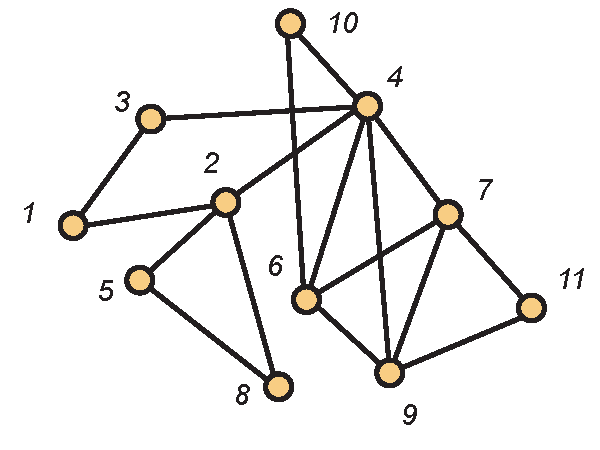
\includegraphics[width=2.5in]{graphs-figs/eulerian_graph}

  \caption{An Eulerian Graph}
  \label{fig:graphs:eulerexample}
\end{figure}
You should note that \autoref{thm:eulerian} holds for loopless graphs
in which multiple edges are allowed.  Euler used his theorem to show
that the multigraph of K\"onigsberg shown in
\autoref{fig:bridges-graph}, in which each land mass is a vertex and
each bridge is an edge, is \textit{not} eulerian, and thus the
citizens could not find the route they desired. (Note that in
\autoref{fig:bridges-graph} there are multiple edges between the same
pair of vertices.)

\begin{figure}[h]
  \centering
  
\includegraphics{graphs-figs/konigsberg_graph}
  \caption{The multigraph of K\"onigsberg's bridges}
  \label{fig:bridges-graph}
\end{figure}

A graph $\GVE$ is said to be \textit{hamiltonian} if there exists a
sequence $(x_1,x_2,\dots,x_n)$ so that
\begin{enumerate}
\item every vertex of $\bfG$ appears exactly once in the sequence;
\item $x_1x_n$ is an edge of $\bfG$; and
\item for each $i=1,2,\dots,n-1$, $x_ix_{i+1}$ is an edge in $\bfG$.
\end{enumerate}

The first graph shown in \autoref{fig:eulham} both eulerian and
hamiltonian.  The second is hamiltonian but not eulerian.
\begin{figure}
\begin{center}
\includegraphics*[width=3.55in]{graphs-figs/eulerian_hamiltonian_crop}
\caption{\label{fig:eulham}Eulerian and Hamiltonian Graphs}
\end{center}
\end{figure}

In \autoref{fig:petersen}, we show a famous graph known
as the Petersen graph. It is not hamiltonian.
% Might we want to include the proof of this?
\begin{figure}
\begin{center}
\includegraphics*[width=0.56\textwidth]{graphs-figs/petersen_graph}
\caption{\label{fig:petersen}The Petersen Graph}
\end{center}
\end{figure}

Unlike the situation with eulerian circuits, there is no
known method for quickly determining whether a graph is
hamiltonian.  However, there are a number of interesting
conditions which are sufficient.  Here is one quite well
known example, due to Dirac.

\begin{theorem}\label{thm:graphs:dirac}
If $\bfG$ is a graph on $n$ vertices and each vertex
in $\bfG$ has at least $\lceil \frac{n}{2}\rceil$ neighbors,
then $\bfG$ is hamiltonian.
\end{theorem}

\begin{proof}
Suppose the theorem fails and let $n$ be the least positive
integer for which there exists a graph $\bfG$ on $n$ vertices
so that each vertex in $\bfG$ has at least $\lceil n/2\rceil$
neighbors, yet there is no hamiltonian cycle in $\bfG$. Clearly,
$n\ge4$.

Now let $t$ be the largest integer for which $\bfG$ has
a path $P=(x_1,x_2,\dots,x_t)$ on $t$ vertices.  Clearly all
neighbors of both $x_1$ and $x_t$ appear on this path.  By
the pigeon hole principle, there is some integer $i$ with
$1\le i<t$ so that $x_1x_{i+1}$ and $x_{i}x_t$ are edges
in $\bfG$.  However, this implies that
\[
C=(x_1,x_2,x_3,\dots,x_i,x_t,x_{t-1},x_{t-2},\dots,x_{i+1})
\]
is a cycle of length $t$ in $\bfG$. In turn, this 
requires $\lceil n/2\rceil < t<n$.  But if $y$ is any vertex
not on the cycle, then $y$ must have a neighbor on $C$, which
implies that $\bfG$ has a path on $t+1$ vertices.  The contradiction
completes the proof.
\end{proof}

\section{Graph Coloring}\label{s:graphs:color}

Let's return now to the subject of
\hyperref[ex:radiostations]{Example~\ref*{ex:radiostations}},
assigning frequencies to radio stations so that they don't
interfere. The first thing that we will need to do is to turn the map
of radio stations into a suitable graph, which should be pretty
natural at this juncture. We define a graph $\GVE$ in which $V$ is the
set of radio stations and $xy\in E$ if and only if radio station $x$
and radio station $y$ are within $200$ miles of each other. With this
as our model, then we need to assign different frequencies to two
stations if their corresponding vertices are joined by an edge. This
leads us to our next topic, coloring graphs.

When $\GVE$ is a graph and $C$ is a set of elements called
\textit{colors}, a \textit{proper coloring} of $\bfG$ is a function
$\phi:V\to C$ such that if $\phi(x)\neq \phi(y)$ whenever $xy$ is an
edge in $\bfG$.  The least $t$ for which $\bfG$ has a proper coloring
using a set $C$ of $t$ colors is called the \textit{chromatic number}
of $\bfG$ and is denoted $\chi(\bfG)$.  In \autoref{fig:graphs:chi4},
we show a proper coloring of a graph using $5$ colors. Now we can see
that our radio frequency assignment problem is the much-studied
question of finding the chromatic number of an appropriate graph.
\begin{figure}[h]
\begin{center}
\includegraphics*[scale=0.63]{graphs-figs/chi4}
\caption{\label{fig:graphs:chi4}A proper coloring using $5$ colors}
\end{center}
\end{figure}

\begin{discussion}
  Everyone agrees that the graph $\bfG$ in \autoref{fig:graphs:chi4}
  has chromatic number at most $5$. However, there's a bit of debate
  going on about if $\chi(\bfG)=5$. Bob figures the authors would not
  have used five colors if they didn't need to. Carlos says he's glad
  they're having the discussion, since all having a proper coloring
  does is provide them with an upper bound on $\chi(\bfG)$. Bob sees
  that the graph has a vertex of degree $5$ and claims that must mean
  $\chi(\bfG)=5$. Alice groans and draws a graph with $101$ vertices,
  one of which has degree $100$, but with chromatic number $2$. Bob is
  shocked, but agrees with her. Xing wonders if the fact that the
  graph does not contain a $\bfK_3$ has any bearing on the chromatic
  number. Dave's in a hurry to get to the gym, but on his way out the
  door he says they can get a proper $4$-coloring pretty easily, so
  $\chi(\bfG)\leq 4$. The rest decide it's time to keep reading.
 \begin{itemize}
  \item What graph did Alice draw that shocked Bob?
  \item What changes did Dave make to the coloring in
    \autoref{fig:graphs:chi4} to get a proper coloring using four
    colors?
  \end{itemize}
\end{discussion}

\subsection{Bipartite Graphs}

A graph $\GVE$ with $\chi(\bfG)\le 2$ is called a $2$-\textit{colorable} graph. 
Recognizing $2$-colorable graphs is easy.

\begin{theorem}\label{thm:graphs:bipartite}
  A graph is $2$-colorable if and only if it does not contain an odd
  cycle.
\end{theorem}

\begin{proof}
  Clearly a graph containing an odd cycle cannot be $2$-colorable.
  For the converse, let $\bfG$ be a graph which does not contain
  an odd cycle.   For each component $C$ of $\bfG$, we choose
  an arbitrary vertex $r_C$ from $C$ and color all such vertices
  with color $1$.  Then for each component $C$ and each vertex
  $y\in C$ with $y\neq r_C$, let $P=(r_C=x_1,x_2,\dots,x_t=y)$ be
  a shortest path from $r_C$ to $y$.  Assign $y$ color $1$ if
  $t$ is odd and color~$2$ if $t$ is even.  It is easy to see that
  this determines a $2$-coloring of $\bfG$.
\end{proof}

A graph $\bfG$ is called a bipartite graph when there is
a partition of the vertex $V$ into two sets $A$ and $B$ 
so that the subgraphs induced by $A$ and $B$ are independent graphs, 
i.e., no edge of $\bfG$ has both of its endpoints in $A$ or in $B$. 
Evidently, bipartite graphs are $2$-colorable.  On the other hand,
when a $2$-colorable graph is disconnected, there is more than
one way to define a suitable partition of the vertex set into
two independent sets.

Bipartite graphs are commonly used as models when there are two
distinct types of objects being modeled and connections are only
allowed between two objects of different types.  For example,
on one side, list candidates who attend a career fair and on the
other side list the available positions.  The edges might naturally
correspond to candidate/position pairs which link a person to
a responsibility they are capable of handling.

As a second example, a
bipartite graph could be used to visualize the languages spoken by a
group of students. The vertices on one side would be the students with the
languages listed on the other side.  We would then have an edge $xy$ when
student $x$ spoke language $y$.
A concrete example of this graph for our favorite group of students is
shown in \autoref{fig:graphs:languages}, although Alice isn't so
certain there should be an edge connecting Dave and English.

\begin{figure}[b]
  \centering
  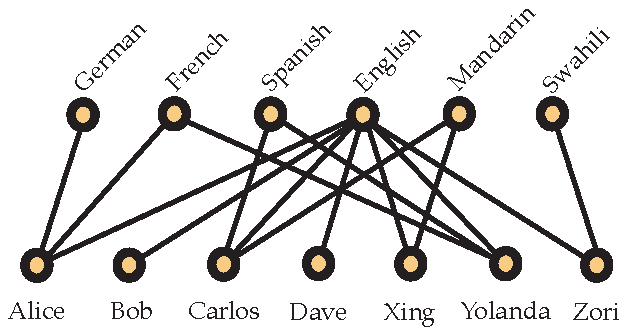
\includegraphics[scale=0.63]{graphs-figs/languages}
  \caption{A bipartite graph}
  \label{fig:graphs:languages}
\end{figure}

One special class of bipartite graphs that bears mention is the class
of \emph{complete bipartite graphs}. The complete bipartite graph
$\bfK_{m,n}$ has vertex set $V=V_1\cup V_2$ with $|V_1|=m$ and
$|V_2|=n$. It has an edge $xy$ if and only if $x\in V_1$ and $y\in
V_2$. The complete bipartite graph $\bfK_{3,3}$ is shown in \autoref{fig:graphs:k33}.

\begin{figure}[h]
  \centering
  
\includegraphics{graphs-figs/k33_rotated}
  \caption{The complete bipartite graph $\bfK_{3,3}$}
  \label{fig:graphs:k33}
\end{figure}

\subsection{Cliques and Chromatic Number}

A \textit{clique} in a graph $\GVE$ is a set $K\subseteq V$ such that
the subgraph induced by $K$ is isomorphic to the complete graph
$\bfK_{|K|}$. Equivalently, we can say that every pair of vertices in
$K$ are adjacent. The \textit{maximum clique size} or \textit{clique
  number} of a graph $\bfG$, denoted $\omega(\bfG)$, is the largest
$t$ for which there exists a clique $K$ with $|K|=t$.  For example,
the graph in \autoref{fig:graphs:eulerexample} has clique number $4$
while the graph in \autoref{fig:graphs:chi4} has maximum clique
size~$2$.

For every graph $\bfG$, it is obvious that $\chi(\bfG)\ge
\omega(\bfG)$.  On the other hand, the inequality may be far from
tight. Before proving showing how bad it can be, we need to introduce
a more general version of the
\hyperref[prop:pigeon]{Pigeon Hole Principle
  (Proposition~\ref*{prop:pigeon})}. Consider a function $f\colon X\to
Y$ with $|X| = 2|Y|+1$. Since $|X|>|Y|$, the Pigeon Hole Principle
as stated in \autoref{ch:basics} only tells us that there are distinct
$x,x'\in X$ with $f(x)=f(x')$. However, we can say more here. Suppose
that each element of $Y$ has at most two elements of $X$ mapped to
it. Then adding up the number of elements of $X$ based on how many are
mapped to each element of $Y$ would only allow $X$ to have (at most)
$2|Y|$ elements. Thus, there must be $y\in Y$ so that there are three
distinct elements $x,x',x''\in X$ with $f(x)=f(x')=f(x'')=y$. This
argument generalizes to give the following version of the Pigeon Hole
Principle:

\begin{proposition}\label{prop:graphs:pigeon-general}
  If $f\colon X\to Y$ is a function and $|X|\geq (m-1)|Y|+1$, then
  there exists an element $y\in Y$ and distinct elements
  $x_1,\dots,x_m \in X$ so that $f(x_i)=y$ for $i=1,\dots,m$.
\end{proposition}

We are now prepared to present the following proposition showing that
clique number and chromatic number need not be close at all.

\begin{proposition}\label{prop:triangle-free}
  For every $t\ge3$, there exists a graph $\bfG_t$ so that
  $\chi(\bfG_t)=t$ and $\omega(\bfG_t)=2$
\end{proposition}

\begin{proof}[Proof (J. Kelly and L. Kelly)]
  We proceed by induction on $t$. For $t=3$, we take $\bfG_3$ to be
  the cycle $\bfC_5$ on five vertices.  Now assume that for some
  $t\ge3$, we have determined the graph $\bfG_t$.  Suppose that
  $\bfG_t$ has $n_t$ vertices.  Label the vertices of $\bfG_t$ as
  $x_1,x_2,\dots,x_{n_t}$.  Construct $\bfG_{t+1}$ as follows.  Begin
  with an independent set $I$ of cardinality $t(n_t-1)+1$.  For every
  subset $S$ of $I$ with $|S|=n_t$, label the elements of $S$ as
  $y_1,y_2,\dots,y_{n_t}$.  For this particular $n_t$-element subset
  attach a copy of $\bfG_t$ with $y_i$ adjacent to $x_i$ for
  $i=1,2,\dots,n_t$.  Vertices in copies of $\bfG_t$ for distinct
  $n_t$-element subsets of $I$ are nonadjacent, and a vertex in $I$
  has at most one neighbor in a particular copy of $\bfG_t$.

  To see that $\omega(\bfG_{t+1})=2$, it will suffice to argue that
  $\bfG_{t+1}$ contains no triangle ($\bfK_3$).  Since $\bfG_t$ is
  triangle-free, any triangle in $\bfG_{t+1}$ must contain a vertex of
  $I$. Since none of the vertices of $I$ are adjacent, any triangle in
  $\bfG_{t+1}$ contains only one point of $I$. Since each vertex of
  $I$ is adjacent to at most one vertex of any fixed copy of $\bfG_t$,
  if $y\in I$ is part of a triangle, the other two vertices must come
  from distinct copies of $\bfG_t$. However, vertices in different
  copies of $\bfG_t$ are not adjacent, so
  $\omega(\bfG_{t+1})=2$. Notice that $\chi(\bfG_{t+1})\ge t$ since
  $\bfG_{t+1}$ contains $\bfG_t$.  On the other hand,
  $\chi(\bfG_{t+1})\le t+1$ since we may use $t$ colors on the copies
  of $\bfG_t$ and a new color on the independent set $I$.  To see that
  $\chi(\bfG_{t+1})=t+1$, observe that if we use only $t$ colors, then
  by the generalized Pigeon Hole Principle, there is an $n_t$-element
  subset of $I$ in which all vertices have the same color.  Then this
  color cannot be used in the copy of $\bfG_t$ which is attached to
  that $n_t$-element subset.
\end{proof}

Here is another argument for the same result.

\begin{proof}[Proof (J. Mycielski)]
  We again start with $\bfG_3$ as the cycle $\bfC_5$.  As before we
  assume that we have constructed for some $t\ge3$ a graph $\bfG_t$
  with $\omega(\bfG_t)=2$ and $\chi(\bfG_t) = t$.  Again, label the
  vertices of $\bfG_t$ as $x_1,x_2,\dots,x_{n_t}$.  To construct
  $\bfG_{t+1}$, we now start with an independent set $I$, but now $I$
  has only $n_t$ points, which we label as $y_1,y_2,\dots,y_{n_t}$.  We
  then add a copy of $\bfG_t$ with $y_i$ adjacent to $x_j$ if and only
  if $x_i$ is adjacent to $x_j$.  Finally, attach a new vertex $z$
  adjacent to all vertices in $I$.

  Clearly, $\omega(\bfG_{t+1})=2$.  Also,
  $\chi(\bfG_{t+1})\ge t$, since it contains $\bfG_t$ as a subgraph.
  Furthermore,
  $\chi(\bfG_{t+1})\leq t+1$, since we can color $\bfG_t$ with colors
  from $\{1,2,\dots,t\}$, use color $t+1$ on the independent set $I$,
  and then assign color~$1$ to the new vertex $z$. We claim that in fact
  $\chi(\bfG_{t+1})=t+1$. Suppose not. Then we must have
  $\chi(\bfG_{t+1})=t$.  Let $\phi$ be a proper
  coloring of $\bfG_{t+1}$.  Without loss of generality, $\phi$ uses
  the colors in $\{1,2,\dots,t\}$ and $\phi$ assigns color~$t$ to $z$.
  Then consider the nonempty set $S$ of vertices in the copy of
  $\bfG_t$ to which $\phi$ assigns color $t$.  For each $x_i$ in $S$,
  change the color on $x_i$ so that it matches the color assigned to
  $y_i$ by $\phi$, which cannot be $t$, as $z$ is colored $t$.  What
  results is a proper coloring of the copy of $\bfG_t$ with only $t-1$
  colors since $x_i$ and $y_i$ are adjacent to the same vertices of
  the copy of $\bfG_t$.  The contradiction shows that
  $\chi(\bfG_{t+1})=t+1$, as claimed.
\end{proof}

Since a $3$-clique looks like a triangle,
\hyperref[prop:triangle-free]{Proposition~\ref*{prop:triangle-free}}
is often stated as ``There exist triangle-free graphs with large
chromatic number.'' As an illustration of the construction in the
proof of Mycielski, we again refer to \autoref{fig:graphs:chi4}.  The
graph shown is $\bfG_4$. We will return to the topic of graphs with
large chromatic number in \autoref{s:probmeth:girth} where we show
that are there graphs with large chromatic number which lack not only
cliques of more than two vertices but also \emph{cycles} of less than
$g$ vertices for \emph{any} value of $g$. In other words, there is a
graph $\bfG$ with $\chi(\bfG)=10^6$ but no cycle with fewer than
$10^{10}$ vertices!

\subsection{Can We Determine Chromatic Number?}

Suppose you are given a graph $\bfG$. It's starting to look like it is
not easy to find an algorithm that answers the question ``Is
$\chi(\bfG)\leq t$?'' It's easy to verify a certificate (a proper
coloring using at most $t$ colors), but how could you even find a
proper coloring, not to mention one with the fewest number of colors?
Similarly for the question ``Is $\omega(\bfG)\geq k$?'', it is easy to
verify a certificate. However, finding a maximum clique appears to be
a very hard problem. Of course, since the gap between $\chi(\bfG)$ and
$\omega(\bfG)$ can be arbitrarily large, being able to find one value
would not (generally) help in finding the value of the other. No
polynomial-time algorithm is known for either of these problems, and
many believe that no such algorithm exists. In this subsection, we
look at one approach to finding chromatic number and see a case where
it does work efficiently.

A very na\"ive algorithmic way to approach graph coloring is the First
Fit, or ``greedy'', algorithm. For this algorithm, fix an ordering of
the vertex set $V=\{v_1,v_2,\dots v_n\}$. We define the coloring
function $\phi$ one vertex at a time in increasing order of
subscript. We begin with $\phi(v_1)=1$ and then we define
$\phi(v_{i+1})$ (assuming vertices $v_1,v_2,\dots,v_i$ have been
colored) to be the least positive integer color that has not already
been used on any of its neighbors in the set $\{v_1,\dots v_i\}$.

\begin{figure}
  \centering
  \begin{picture}(0,0)
    \put(0,76){\raisebox{0mm}[0mm][0mm]{\makebox[0mm]{$v_1$}}}%
    \put(0,52){\raisebox{0mm}[0mm][0mm]{\makebox[0mm]{$v_3$}}}%
    \put(0,29){\raisebox{0mm}[0mm][0mm]{\makebox[0mm]{$v_5$}}}%
    \put(0,7){\raisebox{0mm}[0mm][0mm]{\makebox[0mm]{$v_7$}}}%
    \put(65,76){\raisebox{0mm}[0mm][0mm]{\makebox[0mm]{$v_2$}}}%
    \put(65,52){\raisebox{0mm}[0mm][0mm]{\makebox[0mm]{$v_4$}}}%
    \put(65,29){\raisebox{0mm}[0mm][0mm]{\makebox[0mm]{$v_6$}}}%
    \put(65,7){\raisebox{0mm}[0mm][0mm]{\makebox[0mm]{$v_8$}}}%
    \put(113,76){\raisebox{0mm}[0mm][0mm]{\makebox[0mm]{$v_1$}}}%
    \put(113,52){\raisebox{0mm}[0mm][0mm]{\makebox[0mm]{$v_2$}}}%
    \put(113,29){\raisebox{0mm}[0mm][0mm]{\makebox[0mm]{$v_3$}}}%
    \put(113,7){\raisebox{0mm}[0mm][0mm]{\makebox[0mm]{$v_4$}}}%
    \put(178,76){\raisebox{0mm}[0mm][0mm]{\makebox[0mm]{$v_5$}}}%
    \put(178,52){\raisebox{0mm}[0mm][0mm]{\makebox[0mm]{$v_6$}}}%
    \put(178,29){\raisebox{0mm}[0mm][0mm]{\makebox[0mm]{$v_7$}}}%
    \put(178,7){\raisebox{0mm}[0mm][0mm]{\makebox[0mm]{$v_8$}}}%
  \end{picture}
  
\includegraphics{graphs-figs/k44-M_crop}\hspace{.75in}
\includegraphics{graphs-figs/k44-M_crop}
  \caption{Two orderings of the vertices of a bipartite graph.}
  \label{fig:k44minus}
\end{figure}
\autoref{fig:k44minus} shows two different orderings of the same
graph. \hyperref[ex:graphs:first-fit-color]{Exercise~\ref*{ex:graphs:first-fit-color}}
demonstrates that the ordering of $V$ is vital to the ability of the
First Fit algorithm to color $\bfG$ using $\chi(\bfG)$ colors. In
general, finding an optimal ordering is just as difficult as coloring
$\bfG$. Thus, this very simple algorithm does not work well in
general. However, for some classes of graphs, there is a ``natural''
ordering that leads to optimal performance of First Fit. Here is one
such example---one that we will study again in the next chapter in a
different context.

Given an indexed family of sets $\cgF=\{S_\alpha:\alpha\in V\}$, we
associate with $\cgF$ a graph $\bfG$ defined as follows.  The vertex
set of $\bfG$ is the set $V$ and vertices $x$ and $y$ in $V$ are
adjacent in $\bfG$ if and only if $S_x\cap S_y \neq\emptyset$.  We
call $\bfG$ an \textit{intersection graph}.  It is easy to see that
every graph is an intersection graph (\emph{why?}), so it makes sense
to restrict the sets which belong to $\cgF$.  For example, we call
$\bfG$ an \textit{interval graph} if it is the intersection graph of a
family of closed intervals of the real line $\reals$. For example, in
\autoref{fig:graphs:interval-graph}, we show a collection of six
intervals of the real line on the left. On the right, we show the
corresponding interval graph having an edge between vertices $x$ and
$y$ if and only if intervals $x$ and $y$ overlap.

\begin{figure}
  \centering
  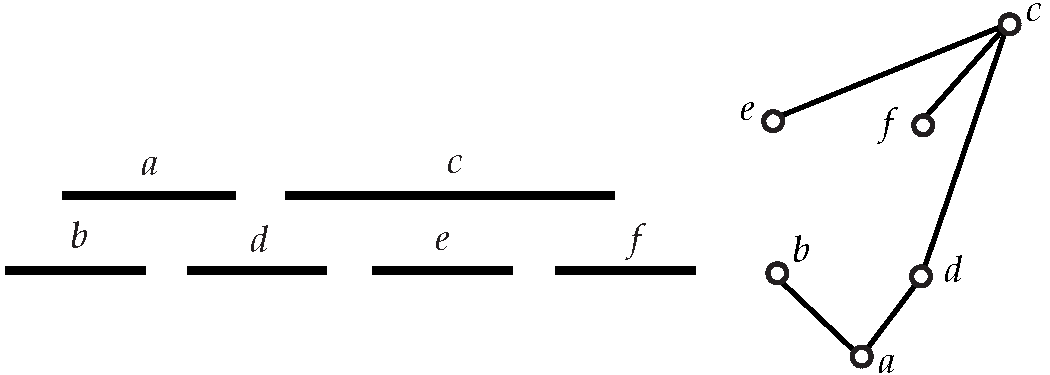
\includegraphics[scale=0.5]{graphs-figs/interval-graph}
  \caption{A collection of intervals and its interval graph}
  \label{fig:graphs:interval-graph}
\end{figure}

\begin{theorem}
  \label{thm:intgraphcol}If $\GVE$ is an interval graph, then
  $\chi(\bfG)=\omega(\bfG)$.
\end{theorem}

\begin{proof}
  For each $v\in V$, let $I(v)=[a_v,b_v]$ be a closed interval of the
  real line so that $uv$ is an edge in $\bfG$ if and only if $I(u)\cap
  I(v)\neq\emptyset$. Order the vertex set $V$ as $\{v_1,v_2,\dots
  v_n\}$ such that $a_1\leq a_2\leq \cdots \leq a_n$. (Ties may be
  broken arbitrarily.) Apply the First Fit coloring algorithm to
  $\bfG$ with this ordering on $V$. Now when the First Fit coloring
  algorithm colors $v_i$, all of its neighbors have left end point at
  most $a_i$. Since they are neighbors of $v_i$, however, we know that
  their right endpoints are all at least $a_i$. Thus, $v_i$ and its
  previously-colored neighbors form a clique. Hence, $v_i$ is adjacent
  to at most $\omega(\bfG)-1$ other vertices that have already been
  colored, so when the algorithm colors $v_i$, there will be a color
  from $\{1,2,\dots,\omega(\bfG)\}$ not already in use on its
  neighbors.  The algorithm will assign $v_i$ the smallest such
  color. Thus, we never need to use more than $\omega(\bfG)$ colors,
  so $\chi(\bfG)=\omega(\bfG)$.
\end{proof}

A graph $\bfG$ is said to be \emph{perfect} if
$\chi(\bfH)=\omega(\bfH)$ for every induced subgraph $\bfH$. Since an
induced subgraph of an interval graph is an interval graph,
\autoref{thm:intgraphcol} shows interval graphs are perfect. The study
of perfect graphs originated in connection with the theory of
communications networks and has proved to be a major area of research
in graph theory for many years now.

\section{Planar Graphs}\label{s:graphs:planar}

Let's return to the problem of providing lines for water, electricity,
and natural gas to three homes which we discussed in the introduction
to this chapter. How can we model this problem using a graph? The best
way is to have a vertex for each utility and a vertex for each of the
three homes. Then what we're asking is if we can draw the graph that
has an edge from each utility to each home so that none of the edges
cross. This graph is shown in \autoref{fig:graphs:utils}. You should
recognize it as the complete bipartite graph $\bfK_{3,3}$ we
introduced earlier in the chapter.
\begin{figure}
  \centering
  \begin{overpic}{graphs-figs/k33}
    \put(-25,92){\small Water}
    \put(-43,50){\small Electricity}
    \put(-53,5){\small Natural gas}
    \put(92,92){\small Home 1}
    \put(92,50){\small Home 2}
    \put(92,5){\small Home 3}
  \end{overpic}
  \caption{A graph of connecting homes to utilities}
  \label{fig:graphs:utils}
\end{figure}

While this example of utility lines might seem a bit contrived, since
there's really no good reason that the providers can't bury their
lines at different depths, the question of whether a graph can be
drawn in the plane such that edges intersect only at vertices is a
long-studied question in mathematics that does have useful
applications. One area where it arises is in the design of microchips
and circuit boards. In those contexts, the material is so thin that
the option of placing connections at different depths either does not
exist or is severely restricted. There is much deep mathematics that
underlies this area, and this section is intended to introduce a few
of the key concepts.

By a \textit{drawing} of a graph, we mean a way of associating its
vertices with points in the Cartesian plane $\reals^2$ and its edges
with simple polygonal arcs whose endpoints are the points associated
to the vertices that are the endpoints of the edge. You can think of a
polygonal arc as just a finite sequence of line segments such that the
endpoint of one line segment is the starting point of the next line
segment, and a simple polygonal arc is one that does not cross
itself. (Our choice of polygonal arcs rather than arbitrary curves
actually doesn't cause an impediment, since by taking very, very, very
short line segments we can approximate any curve.) A \textit{planar
  drawing} of a graph is one in which the polygonal arcs corresponding
to two edges intersect only at a point corresponding to a vertex to
which they are both incident. A graph is \textit{planar} if it has a
planar drawing. A \textit{face} of a planar drawing of a graph is a
region bounded by edges and vertices and not containing any other
vertices or edges.

\autoref{fig:planar} shows a planar drawing of a graph with $6$
vertices and $9$ edges. Notice how one of the edges is drawn as a true
polygonal arc rather than a straight line segment. This drawing
determines $5$ regions, since we also count the unbounded region that
surrounds the drawing.
\begin{figure}[b]
  \centering
  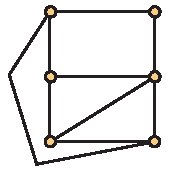
\includegraphics{graphs-figs/planar_graph}
  \caption{A planar drawing of a graph}
  \label{fig:planar}
\end{figure}
\autoref{fig:k4-planar} shows a planar drawing of the complete graph
$\bfK_4$. There are $4$ vertices, $6$ edges, and $4$ faces in the
drawing.
\begin{figure}[ht]
  \centering
  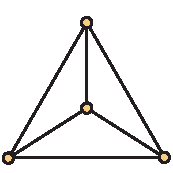
\includegraphics{graphs-figs/k4_planar}
  \caption{A planar drawing of $\bfK_4$}
  \label{fig:k4-planar}
\end{figure}
What happens if we compute the number of vertices minus the number of
edges plus the number of faces for these drawings? We have
\begin{align*}
  6-9+5 &= 2\\
  4-6+4 &=2
\end{align*}
While it might seem like a coincidence that this computation results
in $2$ for these planar drawings, there's a more general principle at
work here, and in fact it holds for \emph{any} planar drawing of
\emph{any} planar graph.

\begin{theorem}[Euler]
  Let $\bfG$ be a connected planar graph with $n$ vertices and $m$
  edges. Every planar drawing of $\bfG$ has $f$ faces, where $f$
  satisfies
  \[n-m+f=2.\]
\end{theorem}

The number $2$ here actually results from a fundamental property of
the plane, and there are a corresponding theorems for other
surfaces. However, we only need the result as stated above.

\begin{proof}
  Our proof is by induction on the number $m$ of edges. If $m=0$, then
  since $\bfG$ is connected, our graph has a single vertex, and so
  there is one face. Thus $n-m+f = 1-0+1=2$ as needed. Now suppose
  that we have proven Euler's formula for all graphs with less than
  $m$ edges and let $\bfG$ have $m$ edges. Pick an edge $e$ of
  $\bfG$. What happens if we form a new graph $\bfG'$ by deleting $e$
  from $\bfG$? If $\bfG'$ is connected, our inductive hypothesis
  applies. Say that $\bfG'$ has $n'$ vertices, $m'$ edges, and $f'$
  faces. Then by induction, these numbers satisfy
  \[n'-m'+f'=2.\]
  Since we only deleted one edge, $n'=n$ and $m'=m-1$. What did the
  removal of $e$ do to the number of faces? In $\bfG'$ there's a new
  face that was formerly two faces divided by $e$ in $\bfG$. Thus,
  $f'=f-1$. Substituting these into $n'-m'+f'=2$, we have
  \[n-(m-1)+(f-1)=2 \iff n-m+f=2.\]
  Thus, if $\bfG'$ is connected, we are done. If $\bfG'$ is
  disconnected, however, we cannot apply the inductive assumption to
  $\bfG'$ directly. Fortunately, since we removed only one edge,
  $\bfG'$ has two components, which we can view as two connected
  graphs $\bfG'_1$ and $\bfG'_2$. Each of these has fewer than $m$
  edges, so we may apply the inductive hypothesis to them. For
  $i=1,2$, let $n'_i$ be the number of vertices of $\bfG'_i$, $m'_i$
  the number of edges of $\bfG'_i$, and $f'_i$ the number of faces of
  $\bfG'_i$. Then by induction we have
  \[n'_1 - m'_1 + f'_1 = 2 \quad \text{and}\quad n'_2-m'_2+f'_2 =2.\]
  Adding these together, we have
  \[(n'_1 + n'_2) - (m'_1 + m'_2) + (f'_1 + f'_2) = 4.\]
  But now $n=n'_1 + n'_2$, and $m'_1 + m'_2 = m-1$, so the equality
  becomes
  \[n - (m-1) + (f'_1+f'_2) = 4 \iff n-m + (f'_1 + f'_2) = 3.\]
  The only thing we have yet to figure out is how $f'_1+f'_2$ relates
  to $f$, and we have to hope that it will allow us to knock the $3$
  down to a $2$. Every face of $\bfG'_1$ and $\bfG'_2$ is a face of
  $\bfG$, since the fact that removing $e$ disconnects $\bfG$ means
  that $e$ must be part of the boundary of the unbounded
  face. Further, the unbounded face is counted twice in the sum $f'_1
  + f'_2$, so $f=f'_1 + f'_2 -1$. This gives exactly what we need to
  complete the proof.
\end{proof}

Taken by itself, Euler's formula doesn't seem that useful, since it
requires counting the number of faces in a planar embedding. However,
we can use this formula to get a quick way to determine that a graph
is not planar.  Consider a drawing without edge crossings
of a graph on $n$ vertices and $m$ edges, with $n\ge3$.
 We consider pairs $(e,F)$ where $e$ is an edge of
$\bfG$ and $F$ is a face that has $e$ as part of its boundary. How
many such pairs are there? Let's call the number of pairs $p$. Each
edge can bound either one or two faces, so we have that $p\leq
2m$. We can also bound $p$ by counting the number of pairs in which a
face $F$ appears. Each face is bounded by at least $3$ edges, so it
appears in at least $3$ pairs, and so $p\geq 3f$. Thus $3f\leq 2m$ or
$f\leq 2m/3$. Now, utilizing Euler's formula, we have
\[m = n+f-2 \leq n + \frac{2m}{3} - 2 \iff \frac{m}{3} \leq n-2.\]
Thus, we've proven the following theorem.

\begin{theorem}\label{thm:max-edge-planar}
  A planar graph on $n$ vertices has at most $3n-6$ edges when
 $n\ge 3$.
\end{theorem}

The contrapositive of this theorem, namely that an $n$-vertex graph
with more than $3n-6$ edges is not planar, is usually the most useful
formulation of this result. For instance, we've seen
(\autoref{fig:k4-planar}) that $\bfK_4$ is planar. What about
$\bfK_5$? It has $5$ vertices and $C(5,2)=10 > 9 = 3\cdot 5-6$ edges,
so it is not planar, and thus for $n\geq 5$, $\bfK_n$ is not planar,
since it contains $\bfK_5$. It's important to note that
\autoref{thm:max-edge-planar} is not the be-all, end-all of
determining if a graph is planar. To see this, let's return to the
subject of drawing $\bfK_{3,3}$ in the plane. This graph has $6$
vertices and $9$ edges, so it passes the test of
\autoref{thm:max-edge-planar}. However, if you spend a couple minutes
trying to find a way to draw $\bfK_{3,3}$ in the plane without
any crossing edges, you'll pretty quickly begin to believe that it
can't be done---and you'd be right!

To see why $\bfK_{3,3}$ is not planar, we'll have to return to Euler's
formula, and we again work with edge-face pairs. For $\bfK_{3,3}$, we
see that every edge would have to be part of the boundary of two
faces, and faces are bounded by cycles. Also, since the graph is
bipartite, there are no odd cycles. Thus, counting edge-face pairs
from the edge perspective, we see that there are $2m = 18$ pairs. If
we let $f_k$ be the number of faces bounded by a cycle of length $k$,
then $f= f_4 + f_6$. Thus, counting edge-face pairs from the face
perspective, there are $4f_4 + 6f_6$ pairs. From Euler's formula, we
see that the number of faces $f$ must be $5$, so then $4f_4+6f_6\geq
20$. But from our count of edge-face pairs, we have $2m=4f_4+6f_6$,
giving $18\geq 20$, which is clearly absurd. Thus, $\bfK_{3,3}$ is not
planar.

At this point, you're probably asking yourself ``So what?'' We've
invested a fair amount of effort to establish that $\bfK_5$ and
$\bfK_{3,3}$ are nonplanar. Clearly any graph that contains them is
also nonplanar, but there are a lot of graphs, so you might think that
we could be at this forever. Fortunately, we won't be, since at its
core, planarity really comes down to just these two graphs, as we
shall soon see.

If $\GVE$ is a graph and $uv\in E$, then we may form a new graph
$\bfG'$ called an \textit{elementary subdivision} of $\bfG$ by adding
a new vertex $v'$ and replacing the edge $uv$ by edges $uv'$ and
$v'v$. In other words, $\bfG'$ has vertex set $V'=V\cup\{v'\}$ and
edge set $E'=(E-\{uv\})\cup \{uv',v'v\}$. Two graphs $\bfG_1$ and
$\bfG_2$ are \emph{homeomorphic} if they can be obtained from the same
graph by a (potentially trivial) sequence of elementary subdivisions.

The purpose of discussing homeomorphic graphs is that two homeomorphic
graphs have the same properties when it comes to being drawn in the
plane. To see this, think about what happens to $\bfK_5$ if we form an
elementary subdivision of it via any one of its edges.  Clearly it
remains nonplanar. In fact, if you take any nonplanar graph and form
the elementary subdivision using any one of its edges, the resulting
graph is nonplanar. The following very deep theorem was proved by the
Polish mathematician Kazimierz Kuratowski in 1930. Its proof is beyond
the scope of this text.

\begin{theorem}[Kuratowski]\label{thm:kuratowski}
  A graph is planar if and only if it does not contain a subgraph
  homeomorphic to either $\bfK_5$ or $\bfK_{3,3}$.
\end{theorem}

Kuratowski's Theorem gives a useful way for checking if a graph is
planar. Although it's not always easy to find a subgraph homeomorphic
to $\bfK_5$ or $\bfK_{3,3}$ by hand, there are efficient algorithms
for planarity testing that make use of this characterization. To see
this theorem at work, let's consider the Petersen graph shown in
\autoref{fig:petersen}. The Petersen graph has $10$ vertices and $15$
edges, so it passes the test of \autoref{thm:max-edge-planar}, and our
argument using Euler's formula to prove that $\bfK_{3,3}$ is nonplanar
was complex enough, we probably don't want to try it for the Petersen
graph. To use Kuratowski's Theorem here, we need to decide if we would
rather find a subgraph homeomorphic to $\bfK_5$ or to
$\bfK_{3,3}$. Although the Petersen graph looks very similar to
$\bfK_5$, it's actually simultaneously \emph{too} similar and too
different for us to be able to find a subgraph homeomorphic to
$\bfK_5$, since each vertex has degree $3$. Thus, we set out to find a
subgraph of the Petersen graph homeomorphic to $\bfK_{3,3}$. To do so,
note that $\bfK_{3,3}$ contains a cycle of length $6$ and three edges
that are in place between vertices opposite each other on the
cycle. We identify a six-cycle in the Petersen graph and draw it as a
hexagon and place the remaining four vertices inside the cycle. Such a
drawing is shown in \autoref{fig:petersen-graph-k33}. The subgraph
homeomorphic to $\bfK_{3,3}$ is found by deleting the black vertex, as
then the white vertices have degree two, and we can replace each of
them and their two incident edges (shown in bold) by a single edge.
\begin{figure}
  \centering
  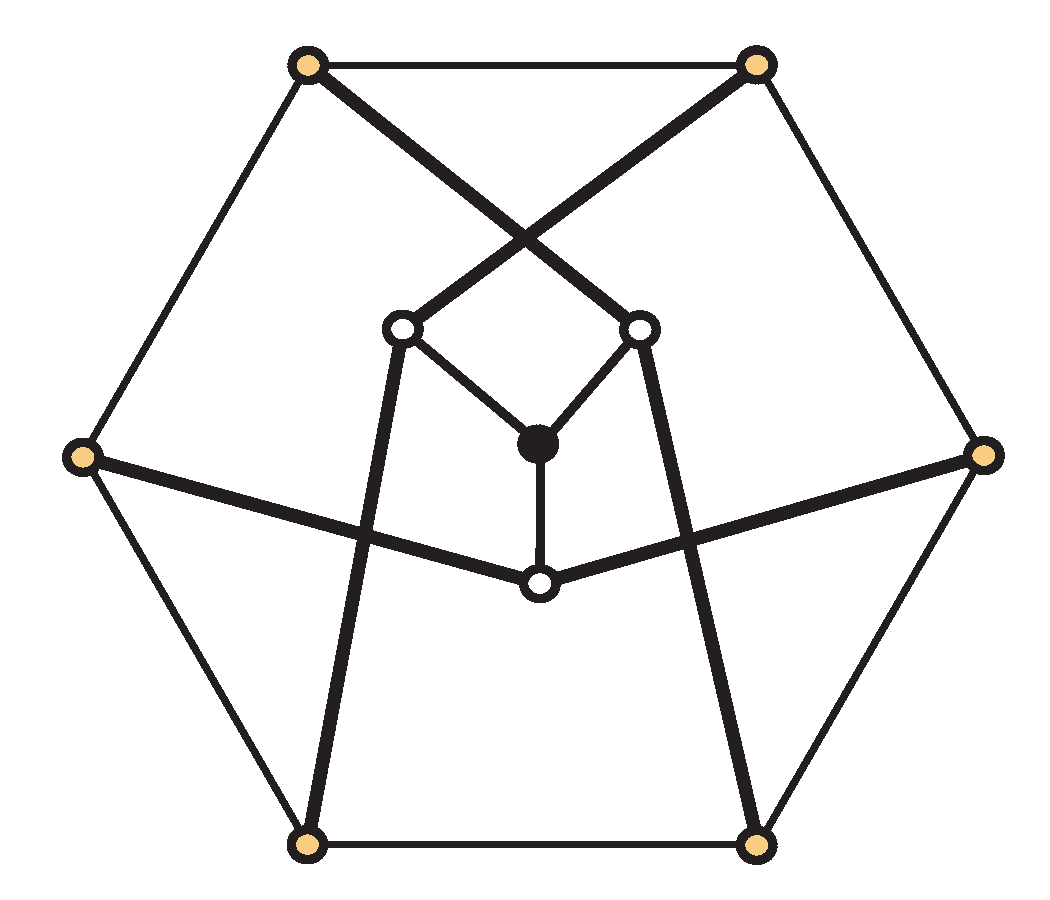
\includegraphics[scale=0.4]{graphs-figs/petersen_graph_k33}
  \caption{A more illustrative drawing of the Petersen graph}
  \label{fig:petersen-graph-k33}
\end{figure}

We close this section with a problem that brings the current section
together with the topic of graph coloring. In 1852 Francis Guthrie, an
Englishman who was at the time studying to be lawyer but subsequently
became a professor of mathematics in South Africa, was trying to color
a map of the counties of England so that any two counties that shared
a boundary segment (meaning they touched in more than a single point)
were colored with different colors. He noticed that he only needed
four colors to do this, and was unable to draw any sort of map that
would require five colors. (He was able to find a map that required
four colors, an example of which is shown in
\autoref{fig:needs-four-colors}.)
\begin{figure}
  \centering
  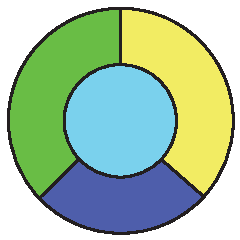
\includegraphics{graphs-figs/needs_four_colors}
  \caption{A map that requires four colors}
  \label{fig:needs-four-colors}
\end{figure}
Could it possibly be true that \emph{every} map could be colored with
only four colors? He asked his brother Frederick Guthrie, who was a
mathematics student at University College, London, about the problem,
and Frederick eventually communicated the problem to Augustus de
Morgan (of de Morgan's laws fame), one of his teachers. It was in this
way that one of the most famous (or infamous) problems, known for a
century as the Four Color Problem and now the Four Color Theorem, in
graph theory was born. De Morgan was very interested in the Four Color
Problem, and communicated it to Sir William Rowan Hamilton,  a
prominent Irish mathematician and the one for whom hamiltonian
cycles are named, but Hamilton did not find the problem
interesting. Hamilton is one of the few people who considered the Four
Color Problem but did not become captivated by it.

We'll continue our discussion of the history of the Four Color Theorem
in a moment, but first, we must consider how we can turn the problem
of coloring a map into a graph theory question. Well, it seems natural
that each region should be assigned a corresponding vertex. We want to
force regions that share a boundary to have different colors, so this
suggests that we should place an edge between two vertices if and only
if their corresponding regions have a common boundary. (As an example,
the map in \autoref{fig:needs-four-colors} corresponds to the graph
$\bfK_4$.) It is not difficult to see that this produces a planar
graph, since we may draw the edges through the common boundary
segment. Furthermore, with a little bit of thought, you should see
that given a planar drawing of a graph, you can create a map in which
each vertex leads to a region and edges lead to common boundary
segments. Thus, the Four Color Problem could be stated as ``Does every
planar graph have chromatic number at most four?''

Interest in the Four Color Problem languished until 1877, when the
British mathematician Arthur Cayley worte a letter to the Royal
Society asking if the problem had been resolved. This brought the
problem to the attention of many more people, and the first ``proof''
of the Four Color Theorem, due to Alfred Bray Kempe, was completed in
1878 and published a year later. It took $11$ years before Percy John
Heawood found a flaw in the proof but was able to salvage enough of it
to show that every planar graph has chromatic number at most five. In
1880, Peter Guthrie Tait, a British physicist best known for his book
\textit{Treatise on Natural Philosophy} with Sir William Thomson (Lord
Kelvin), made an announcement that suggested he had a proof of the
Four Color Theorem utilizing hamiltonian cycles in certain planar
graphs. However, consistent with the way Tait approached some
conjectures in the mathematical theory of knots, it appears that he
subsequently realized around 1883 that he could not prove that the
hamiltonian cycles he was using actually existed and so Tait likely
only believed he had a proof of the Four Color Theorem for a short
time, if at all. However, it would take until 1946 to find a
counterexample to the conjecture Tait had used in his attempt to prove
the Four Color Theorem.

In the first half of the twentieth century, some incremental progress
toward resolving the Four Color Problem was made, but few prominent
mathematicians took a serious interest in it. The final push to prove
the Four Color Theorem came with about at the same time that
the first electronic computers were coming into widespread use in
industry and research. In 1976, two mathematicians at the University
of Illinois announced their computer-assisted proof of the Four Color
Theorem. The proof by Kenneth Appel and Wolfgang Haken led the
University of Illinois to add the phrase ``FOUR COLORS
SUFFICE'' to its postage meter's imprint.\footnote{A photograph of an envelope with such a meter mark
  on it can be found in the book \textit{The Four-Color Theorem:
    History, Topological Foundations, and Idea of Proof} by Rudolf and
  Gerda Fritsch. (Springer, 1998)}

\begin{theorem}[Four Color Theorem]\label{thm:4ct}
  Every planar graph has chromatic number at most four.
\end{theorem}

Appel and Haken's proof of the Four Color Theorem was at a minimum
unsatisfactory for many mathematicians, and to some it simply wasn't a
proof. These mathematicians felt that the using a computer to check
various cases was simply too uncertain; how could you be certain that
the code that checked the 1,482 ``unavoidable configurations'' didn't
contain any logic errors? In fact, there were several mistakes found
in the cases analyzed, but none were found to be fatal flaws. In 1989,
Appel and Haken published a 741-page tome entitled \textit{Every
  Planar Map is Four Colorable} which provided corrections to all
known flaws in their original argument. This still didn't satisfy
many, and in the early 1990's a team consisting of Neil Robertson from
The Ohio State University; Daniel P. Sanders, a graduate student at
the Georgia Institute of Technology; Paul Seymour of
Bellcore; and Robin Thomas from Georgia Tech announced a new proof of
the Four Color Theorem. However, it still required the use of
computers. The proof did gain more widespread acceptance than that of
Appel and Haken, in part because the new proof used fewer than half
($633$) of the number of configurations the Appel-Haken proof used and
the computer code was provided online for anyone to verify. While
still unsatisfactory to many, the proof by Robertson, et al. was
generally accepted, and today the issue of the Four Color Theorem has
largely been put to rest. However, many still wonder if anyone will
ever find a proof of this simple statement that does not require the
assistance of a computer.

\section{Counting Labeled Trees}\label{s:graphs:counting-trees}

How many trees are there with vertex set $[n]=\{1,2,\dots,n\}$? Let
$T_n$ be this number. For $n=1$, there is clearly only one tree. Also,
for $n=2$, there is only one tree, which is isomorphic to $\bfK_2$. In
determining $T_3$, we finally have some work to do; however, there's
not much, since all trees on $3$ vertices are isomorphic to
$\bfP_3$. Thus, there are $T_3=3$ \emph{labeled} trees on $3$
vertices, corresponding to which vertex is the one of degree $2$. When
$n=4$, we can begin by counting the number of nonisomorphic trees and
consider two cases depending on whether the tree has a vertex of
degree $3$.  If there is a vertex of degree $3$, the tree is
isomorphic to $\bfK_{1,3}$ or it does not have a vertex of degree
three, in which case it is isomorphic to $\bfP_4$, since there must be
precisely two vertices of degree $2$ in such a graph. There are four
labelings by $[4]$ for $\bfK_{1,3}$ (choose the vertex of degree
three). How many labelings by $[4]$ are there for $\bfP_4$? There are
$C(4,2)$ ways to choose the labels $i,j$ given to the vertices of
degree $2$ and two ways to select one of the remaining labels to be
made adjacent to $i$. Thus, there are $12$ ways to label $\bfP_4$ by
$[4]$ and so $T_4=16$.

To this point, it looks like maybe there's a pattern forming. Perhaps
it is the case that for all $n\geq 1$, $T_n = n^{n-2}$. This is in
fact the case, but let's see how it works out for $n=5$ before proving
the result in general. What are the nonisomorphic trees on five
vertices? Well, there's $\bfK_{1,4}$ and $\bfP_5$ for sure, and
there's also the third tree shown in \autoref{fig:trees-5verts}. After
thinking for a minute or two, you should be able to convince yourself
that this is all of the possibilities. How many labelings by $[5]$
does each of these have? There are $5$ for $\bfK_{1,4}$ since there
are $5$ ways to choose the vertex of degree $4$. For $\bfP_5$, there
are $5$ ways to choose the middle vertex of the path, $C(4,2)=6$ ways
to label the two remaining vertices of degree $2$ once the middle
vertex is labeled, and then $2$ ways to label the vertices of degree
$1$. This gives $60$ labelings. For the last tree, there are $5$ ways
to label the vertex of degree $3$, $C(4,2)=6$ ways to label the two
leaves adjacent to the vertex of degree $3$, and $2$ ways to label the
remaining two vertices, giving $60$ labelings. Therefore,
$T_5=125=5^3=5^{5-2}$.
\begin{figure}
  \centering
  
\includegraphics{graphs-figs/trees-5verts}
  \caption{The nonisomorphic trees on $n=5$ vertices}
  \label{fig:trees-5verts}
\end{figure}

It turns out that we are in fact on the right track, and we will now
set out to prove the following:
\begin{theorem}[Cayley's Formula]\label{thm:cayley}
  The number $T_n$ of labeled trees on $n$ vertices is $n^{n-2}$.
\end{theorem}
\noindent This result is usually referred to as Cayley's Formula,
although equivalent results were proven earlier by James J.\ Sylvester
(1857) and Carl W.\ Borchardt (1860). The reason that Cayley's name is
most often affixed to this result is that he was the first to state
and prove it in graph theoretic terminology (in 1889). (Although one
could argue that Cayley really only proved it for $n=6$ and then
claimed that it could easily be extended for all other values of $n$,
and whether such an extension can actually happen is open to some
debate.) Cayley's Formula has many different proofs, most of which are
quite elegant. If you're interested in presentations of several
proofs, we encourage you to read the chapter on Cayley's Formula in
\textit{Proofs from THE BOOK} by Aigner, Ziegler, and Hofmann, which
contains four different proofs, all using different proof
techniques. Here we give a fifth proof, due to Pr\"ufer and published
in 1918. Interestingly, even though Pr\"ufer's proof came after much
of the terminology of graph theory was established, he seemed unaware
of it and worked in the context of permutations and his own
terminology, even though his approach clearly includes the ideas of
graph theory. We will use a recursive technique in order to find a
bijection between the set of labeled trees on $n$ vertices and a
natural set of size $n^{n-2}$, the set of strings of length $n-2$
where the symbols in the string come from $[n]$.

We define a recursive algorithm that takes a tree $\bfT$ on $k\geq 2$
vertices labeled by elements of a set $S$ of positive integers of size
$k$ and returns a string of length $k-2$ whose symbols are elements of
$S$. (The set $S$ will usually be $[k]$, but in order to define a
recursive procedure, we need to allow that it be an arbitrary set of
$k$ positive integers.) This string is called the \textit{Pr\"ufer
  code} of the tree $\bfT$. Let $\prufer(\bfT)$ denote the
Pr\"ufer code of the tree $\bfT$, and if $v$ is a leaf of $\bfT$, let
$\bfT-v$ denote the tree obtained from $\bfT$ by removing $v$ (i.e.,
the subgraph induced by all the other vertices). We can then define
$\prufer(\bfT)$ recursively by
\begin{enumerate}
\item If $\bfT\cong \bfK_2$, return the empty string.
\item Else, let $v$ be the leaf of $\bfT$ with the smallest label
  and let $u$ be its unique neighbor. Let $i$ be the label of
  $u$. Return $(i,\prufer(\bfT-v))$.
\end{enumerate}

\begin{example}\label{ex:prufer-code}
  Before using Pr\"ufer codes to prove Cayley's Formula, let's take a
  moment to make sure we understand how they are computed given a
  tree. Consider the $9$-vertex tree $\bfT$ in \autoref{fig:prufer-code}.
  \begin{figure}[h]
    \centering
    \begin{overpic}{graphs-figs/tree-9verts}
      \put(46,2){$1$}
      \put(21,21){$2$}
      \put(62,14.5){$3$}
      \put(36.8,14.5){$4$}
      \put(2,2){$5$}
      \put(9,12){$6$}
      \put(90,12){$7$}
      \put(27.5,5.5){$8$}
      \put(77.3,21){$9$}
    \end{overpic}
    \caption{A labeled $9$-vertex tree}
    \label{fig:prufer-code}
  \end{figure}
How do we compute $\prufer(\bfT)$? Since $\bfT$ has more than two
vertices, we use the second step and find that $v$ is the vertex with
label $2$ and $u$ is the vertex with label $6$, so
$\prufer(\bfT)=(6,\prufer(\bfT-v))$. The graph $\bfT-v$ is
shown in \autoref{fig:prufer-code-delete1}.
  \begin{figure}[h]
    \centering
    \begin{overpic}{graphs-figs/tree-8verts}
      \put(46,2){$1$}
%      \put(21,21){$2$}
      \put(62,14.5){$3$}
      \put(36.8,14.5){$4$}
      \put(2,2){$5$}
      \put(9,12){$6$}
      \put(90,12){$7$}
      \put(27.5,5.5){$8$}
      \put(77.3,21){$9$}
    \end{overpic}
    \caption{The tree $\bfT-v$}
    \label{fig:prufer-code-delete1}
  \end{figure}
  The recursive call $\prufer(\bfT-v)$ returns
  $(6,\prufer(\bfT-v-v'))$, where $v'$ is the vertex labeled
  $5$. Continuing recursively, the next vertex deleted is $6$, which
  appends a $4$ to the string. Then $7$ is deleted, appending
  $3$. Next $8$ is deleted, appending $1$. This is followed by the
  deletion of $1$, appending $4$. Finally $4$ is deleted, appending
  $3$, and the final recursive call has the subtree isomorphic to
  $\bfK_2$ with vertices labeled $3$ and $9$, and an empty string is
  returned. Thus, $\prufer(\bfT)=6643143$.
\end{example}

We're now prepared to give a proof of Cayley's Formula.

\begin{proof}
  It is clear that $\prufer(\bfT)$ takes an $n$-vertex labeled tree
  with labels from $[n]$ and returns a string of length $n-2$ whose
  symbols are elements of $[n]$. What we have yet to do is determine a
  way to take such a string and construct an $n$-vertex labeled tree
  from it. If we can find such a construction, we will have a
  bijection between the set $\mathcal{T}_n$ of labeled trees on $n$
  vertices and the set of strings of length $n-2$ whose symbols come
  from $[n]$, which will imply that $T_n=n^{n-2}$.

  First, let's look at how $\prufer(\bfT)$ behaves. What numbers
  actually appear in the Pr\"ufer code? The numbers that appear in the
  Pr\"ufer code are the labels of the \textit{nonleaf} vertices of
  $\bfT$. The label of a leaf simply cannot appear, since we always
  record the label of the \textit{neighbor} of the leaf we are
  deleting, and the only way we would delete the neighbor of a leaf is
  if that neighbor were also a leaf, which can only happen
  $\bfT\cong\bfK_2$, in which case $\prufer(\bfT)$ simply returns the
  empty string. Thus if $I\subset [n]$ is the set of symbols that
  appear in $\prufer(\bfT)$, the labels of the leaves of $\bfT$ are
  precisely the elements of $[n]-I$.

  With the knowledge of which labels belong to the leaves of $\bfT$ in
  hand, we are ready to use induction to complete the proof. Our goal
  is to show that if given a string $\bfs=s_1s_2\cdots s_{n-2}$ whose
  symbols come from a set $S$ of $n$ elements, there is a unique tree
  $\bfT$ with $\prufer(\bfT) = \bfs$. If $n=2$, the only such string
  is the empty string, so $1$ and $2$ both label leaves and we can
  construct only $\bfK_2$. Now suppose we have the result for some
  $m\geq 2$, and we try to prove it for $m+1$. We have a string $\bfs
  = s_1s_2\cdots s_{m-1}$ with symbols from $[m+1]$. Let $I$ be the
  set of symbols appearing in $\bfs$ and let $k$ be the least element
  of $[m+1]-I$. By the previous paragraph, we know that $k$ is the
  label of a leaf of $\bfT$ and that is unique neighbor is the vertex
  labeled $s_1$. The string $\bfs'=s_2s_3\cdots s_{m-1}$ has length
  $m-2$ and since $k$ does not appear in $\bfs$, its symbols come from
  $S=[m+1]-\{k\}$, which has size $m$. Thus, by induction, there is a
  unique tree $\bfT'$ whose Pr\"ufer code is $\bfs'$. We form $\bfT$
  from $\bfT'$ by attaching a leaf with label $k$ to the vertex of
  $\bfT'$ with label $s_1$ and have a tree of the desired type.
\end{proof}

\begin{example}\label{ex:prufer-code-reverse}
  We close this section with an example of how to take a Pr\"ufer code
  and use it to construct a labeled tree. Consider the string
  $\bfs=75531$ as a Pr\"ufer code. Then the tree $\bfT$ corresponding
  to $\bfs$ has $7$ vertices, and its leaves are labeled $2$, $4$, and
  $6$. The inductive step in our proof attaches the vertex labeled $2$
  to the vertex labeled $7$ in the tree $\bfT'$ with Pr\"ufer code
  $5531$ and vertex labels $\{1,3,4,5,6,7\}$, since $2$ is used to
  label the last vertex added. What are the leaves of $\bfT'$? The
  symbols in $\{4,6,7\}$ do not appear in $5531$, so they must be the
  labels of leaves, and the construction says that we would attach the
  vertex labeled $4$ to the vertex labeled $5$ in the tree we get by
  induction. In \autoref{tab:prufer-code-reverse}, we show how this
  recursive process continues.
  \begin{table}[h]
    \centering
    \begin{tabular}{ccc}
      Pr\"ufer code & Label set & Edge added\\
      75531 & $\{1,2,3,4,5,6,7\}$ & 2--7\\
      5531 & $\{1,3,4,5,6,7\}$ & 4--5\\
      531 & $\{1,3,5,6,7\}$ & 6--5\\
      31 & $\{1,3,5,7\}$ & 5--3\\
      1 & $\{1,3,7\}$ & 3--1\\
      (empty string) & $\{1,7\}$ & 1--7
    \end{tabular}
    \caption{Turning the Pr\"ufer code $75531$ into a labeled tree}
    \label{tab:prufer-code-reverse}
  \end{table}
  We form each row from the row above it by removing the first label
  used on the edge added from the label set and removing the first
  symbol from the Pr\"ufer code. Once the Pr\"ufer code becomes the
  empty string, we know that the two remaining labels must be the
  labels we place on the ends of $\bfK_2$ to start building $\bfT$. We
  then work back up the edge added column, adding a new vertex and the
  edge indicated. The tree we construct in this manner is shown in
  \autoref{fig:prufer-code-reverse}.
  \begin{figure}[h]
    \centering
    \begin{overpic}{graphs-figs/prufer-code-reverse}
      \put(2,21){$4$}
%      \put(21,21){$2$}
      \put(62,14.5){$1$}
      \put(36.8,14.5){$3$}
      \put(2,2){$6$}
      \put(9,12){$5$}
      \put(90,12){$7$}
      \put(93,21){$2$}
    \end{overpic}
    \caption{The labeled tree with Pr\"ufer code $75531$}
    \label{fig:prufer-code-reverse}
  \end{figure}
\end{example}

%\section{Matchings in Graphs}\label{s:graphs:matching}

%This space reserved for a future section focusing on Hall's theorem
%but also talking about general matchings.

\section{A Digression into Complexity Theory}\label{s:graphs:complexity}

We have already introduced in \autoref{ch:basics} a few notions about
efficient algorithms. We also discussed the difficulty of determining
a graph's chromatic number and clique number earlier in this
chapter. We conclude with a brief discussion of some issues involving
computational complexity for other problems discussed in this chapter.

Let's begin with some problems for which there are polynomial-time
algorithms. Suppose you are given a graph on $n$ vertices and asked
whether or not the graph is connected. Here a positive answer can be
justified by providing a spanning tree.  On the other hand, a negative
answer can be justified by providing a partition of the vertex sets
$V=V_1\cup V_2$ with $V_1$ and $V_2$ non-empty subsets and having no
edges with one end-point in $V_1$ and the other in $V_2$. In
\autoref{ch:graphalgorithms} we will discuss two efficient algorithms
that find spanning trees in connected graphs. They can easily be
modified to produce a partition showing the graph is disconnected.

If you are asked whether a connected graph is eulerian, then a
positive answer can be justified by producing the appropriate
sequence. We gave an algorithm to do this earlier in the chapter. A
negative answer can be justified by producing a vertex of odd degree,
and our algorithm will identify such a vertex if it exists. (Depending
on the data structures used to represent the graph, it may be most
efficient to simply look for vertices of odd degree without using the
algorithm to find an eulerian circuit.)

On the surface, the problem of determining if a graph is hamiltonian
looks similar to that of determining if the graph is eulerian. Both
call for a sequence of vertices in which each pair of consecutive
vertices is joined by an edge. Of course, each problem has an
additional requirement on yes certificates. However, justifying a
negative answer to the question of whether a graph is hamiltonian is
not straightforward. \autoref{thm:graphs:dirac} only gives a way to
confirm that a graph \emph{is} hamiltonian; there are many
nonhamiltonian graphs that do not satisfy its hypothesis. At this
time, no one knows how to justify a negative answer---at least not in
the general case.

\section{Discussion}

Over coffee, today's conversation was enthusiastic and heated at
times. Zori got things off with a blast ``I don't think graphs
are of any use at all\dots'' but she wasn't even able to finish
the sentence before Yolanda  uncharacteristically interrupted her with
``You're off base on this one.  I see lots of ways graphs can
be used to model real world problems.  The professor actually
showed us examples back in our first class.  But now that we're
talking in more depth about graphs, things are even clearer.''
Bob added ``These eulerian and hamiltonian cycle problems are
certain to have applications in network routing problems.''
Xing reinforced Bob with ``Absolutely.  There are important
questions in network integrity and information exchange that
are very much the same as these basic problems.'' Alice piled
on ``Even the notion of chromatic number clearly has practical
applications.''  By this time, Zori realized her position was
indefensible but she was reluctant to admit it.  She offered
only a ``Whatever.''

Things quieted down a bit and Dave said ``Finding a hamiltonian
cycle can't be all that hard, if someone guarantees that there
is one.  This extra information must be of value in the search.''
Xing added ``Maybe so.  It seems natural that it should be
easier to find something if you know it's there.''  Alice
asked ``Does the same thing hold for chromatic number?''  Bob
didn't understand her question ``Huh?''  Alice continued,
this time being careful not to even look Bob's way ``I mean
if someone tells you that a graph is $3$-colorable, does that
help you to find a coloring using only three colors?''  Dave
said ``Seems reasonable to me.''

After a brief pause, Carlos offered ``I don't think this extra
knowledge is of any help. I think these problems are pretty hard,
regardless.''  They went back and forth for a while, but in the
end, the only thing that was completely clear is that graphs
and their properties had captured their attention, at least for
now.

\section{Exercises}\label{s:graphs:exercises}
\begin{enumerate}
\item The questions in this exercise pertain to the graph $\bfG$ shown in
  \autoref{fig:graphs:graph_ex}.
  \begin{enumerate}
  \item What is the degree of vertex $8$?
  \item What is the degree of vertex $10$?
  \item How many vertices of degree $2$ are there in $\bfG$? List
    them.
  \item Find a cycle of length $8$ in $\bfG$.
  \item What is the length of a shortest path from $3$ to $4$?
  \item What is the length of a shortest path from $8$ to $7$?
  \item Find a path of length $5$ from vertex $4$ to vertex $6$.
  \end{enumerate}
 \begin{figure}[h]
    \centering
    \includegraphics*[height=1.75in]{graphs-figs/graph_ex}    
    \caption{A graph}
    \label{fig:graphs:graph_ex}
  \end{figure}
\item Draw a graph with $8$ vertices, all of odd degree, that does not
  contain a path of length $3$ or explain why such a graph does not
  exist.
\item Draw a graph with $6$ vertices having degrees $5$, $4$, $4$,
  $2$, $1$, and $1$ or explain why such a graph does not exist.
\item For the next Olympic Winter Games, the organizers wish to expand
  the number of teams competing in curling. They wish to have $14$
  teams enter, divided into two pools of seven teams each. Right now,
  they're thinking of requiring that in preliminary play each team
  will play seven games against distinct opponents. Five of the
  opponents will come from their own pool and two of the opponents
  will come from the other pool. They're having trouble setting up
  such a schedule, so they've come to you. By using an appropriate
  graph-theoretic model, either argue that they cannot use their
  current plan or devise a way for them to do so.
\item For this exercise, consider the graph $\bfG$ in
  \autoref{fig:graphs:subgraphs_ex}.
  \begin{enumerate}
  \item Let $V_1=\{g,j,c,h,e,f\}$ and $E_1=\{ge,jg,ch,ef\}$. Is
    $(V_1,E_1)$ a subgraph of $\bfG$?
  \item Let $V_2=\{g,j,c,h,e,f\}$ and $E_2=\{ge,jg,ch,ef,cj\}$. Is
    $(V_2,E_2)$ a subgraph of $\bfG$?
  \item Let $V_3=\{a,d,c,h,b\}$ and $E_3=\{ch,ac,ad,bc\}$. Is
    $(V_3,E_3)$ an induced subgraph of $\bfG$?
  \item Draw the subgraph of $\bfG$ induced by $\{g,j,d,a,c,i\}$.
  \item Draw the subgraph of $\bfG$ induced by $\{c,h,f,i,j\}$.
  \item Draw a subgraph of $\bfG$ having vertex set $\{e,f,b,c,h,j\}$
    that is \emph{not} an induced subgraph.
  \item Draw a spanning subgraph of $\bfG$ with exactly $10$ edges.
  \end{enumerate}
 \begin{figure}[h]
    \centering
    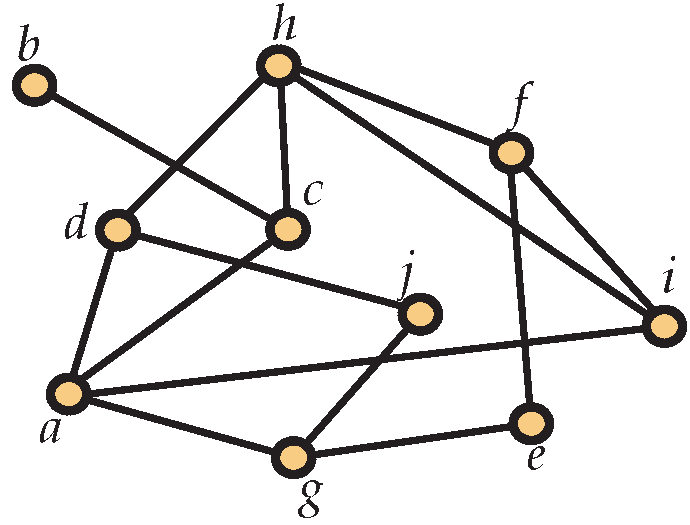
\includegraphics[scale=0.5]{graphs-figs/subgraphs_ex}
    \caption{A graph $\bfG$}
    \label{fig:graphs:subgraphs_ex}
  \end{figure}
\item Prove that every tree on $n$ vertices has exactly $n-1$ edges.
\item \autoref{fig:graphs:isomorphic_ex} contains four graphs on six
  vertices. Determine which (if any) pairs of graphs are
  isomorphic. For pairs that are isomorphic, give an isomorphism
  between the two graphs. For pairs that are not isomorphic, explain
  why.
  \begin{figure}[h]
    \centering
    \begin{overpic}[scale=0.6]{graphs-figs/isomorphic_ex}
      \put(22,47){$\bfG_1$}
      \put(74,47){$\bfG_2$}
      \put(22,-5){$\bfG_3$}
      \put(74,-5){$\bfG_4$}
      \put(4,87){$v_1$} \put(22,87){$v_2$} \put(41,87){$v_3$}
      \put(4,54){$v_4$} \put(22,54){$v_5$} \put(41,54){$v_6$}
      \put(63,96){$u_1$} \put(84,96){$u_2$} \put(99,73){$u_3$}
      \put(89,55){$u_4$} \put(57,55){$u_5$} \put(46.5,73){$u_6$}
      \put(10,41){$w_1$} \put(31.5,41){$w_2$} \put(45.5,20){$w_3$}
      \put(37,3){$w_4$} \put(3,3){$w_5$} \put(-7.5,21){$w_6$}
      \put(56,38.3){$x_1$} \put(74,38.3){$x_2$} \put(92,38.3){$x_3$}
      \put(56,5){$x_4$} \put(74,5){$x_5$} \put(92,5){$x_6$}
    \end{overpic}
    \caption{Are these graphs isomorphic?}
    \label{fig:graphs:isomorphic_ex}
  \end{figure}
\item Find an eulerian circuit in the graph $\bfG$ in
  \autoref{fig:graphs:euler_exercise} or explain why one does not
  exist.
  \begin{figure}[h]
    \begin{center}
      \begin{overpic}[width=4in]{graphs-figs/euler_exercise}
        \put(6,19.5){$1$}
        \put(64.3,5){$2$}
        \put(43.8,15){$3$}
        \put(60,23.5){$4$}
        \put(26,2){$5$}
        \put(21,32){$6$}
        \put(85,9){$$7}
        \put(32.3,26.3){$8$}
        \put(53,-1){$9$}
        \put(42,33){$10$}
        \put(71,26){$11$}
        \put(83,21){$12$}
      \end{overpic}
      \caption{A graph $\bfG$}\label{fig:graphs:euler_exercise}
    \end{center}
  \end{figure}
\item Consider the graph $\bfG$ in \autoref{fig:graphs:euler_hamilton_ex}. Determine if the graph is eulerian. If
  it is, find an eulerian circuit. If it is not, explain why it is
  not. Determine if the graph is hamiltonian. If it is, find a
  hamiltonian cycle. If it is not, explain why it is not.
  \begin{figure}
  \begin{center}
    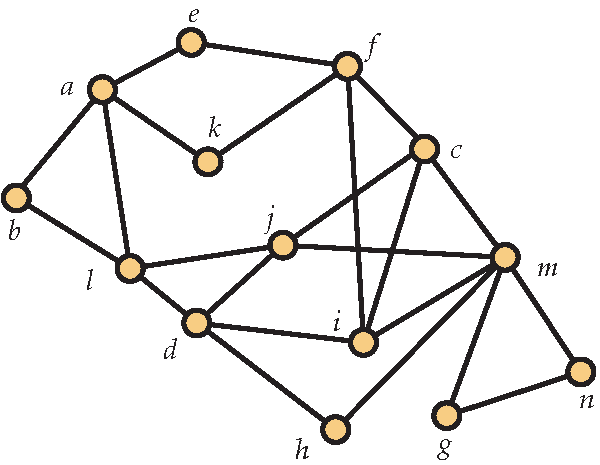
\includegraphics[width=2.5in]{graphs-figs/euler_hamilton_ex}
    \caption{A graph $\bfG$}\label{fig:graphs:euler_hamilton_ex}
 \end{center}
 \end{figure}
\item Explain why the graph $\bfG$ in
  \autoref{fig:graphs:noneuler_exercise} does not have an eulerian
  circuit, but show that by adding a single edge, you can make it
  eulerian.
  \begin{figure}[h]
    \begin{center}
      \begin{overpic}[width=4in]{graphs-figs/noneuler_exercise}
        \put(6,19.5){$1$}
        \put(67,3){$2$}
        \put(48,11){$3$}
        \put(64,33){$4$}
        \put(3,4){$5$}
        \put(21,26){$6$}
        \put(85,9){$$7}
        \put(24.7,12.8){$8$}
        \put(45,-1){$9$}
        \put(32,35){$10$}
        \put(72,24){$11$}
        \put(61,10){$12$}
      \end{overpic}
      \caption{A graph $\bfG$}\label{fig:graphs:noneuler_exercise}
    \end{center}
  \end{figure}
\item An \emph{eulerian trail} is defined in the same manner as an
  euler circuit (see
  \hyperref[def:eulerian-circuit]{page~\pageref*{def:eulerian-circuit}})
  except that we drop the condition that $x_0=x_t$. Prove that a
  graph has an eulerian trail if and only if it is connected and has
  at most two vertices of odd degree.
\item Alice and Bob are discussing a graph that has $17$ vertices and
  $129$ edges. Bob argues that the graph is Hamiltonian, while Alice
  says that he's wrong. Without knowing anything more about the graph,
  must one of them be right? If so, who and why, and if not, why not?
\item Find the chromatic number of the graph $\bfG$ in
  \autoref{fig:graphs:bipartite_ex} and a coloring using $\chi(\bfG)$ colors.
  \begin{figure}[h]
    \centering
    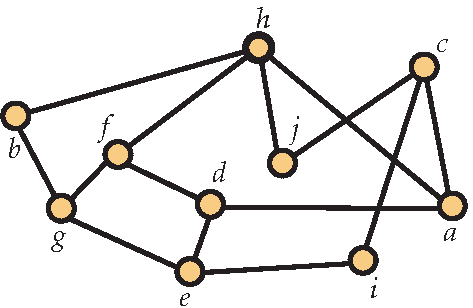
\includegraphics[scale=0.6]{graphs-figs/bipartite_ex}
    \caption{A graph $\bfG$ to color}
    \label{fig:graphs:bipartite_ex}
  \end{figure}
\item Find the chromatic number of the graph $\bfG$ in
  \autoref{fig:graphs:coloring_ex} and a coloring using $\chi(\bfG)$ colors.
  \begin{figure}[h]
    \centering
    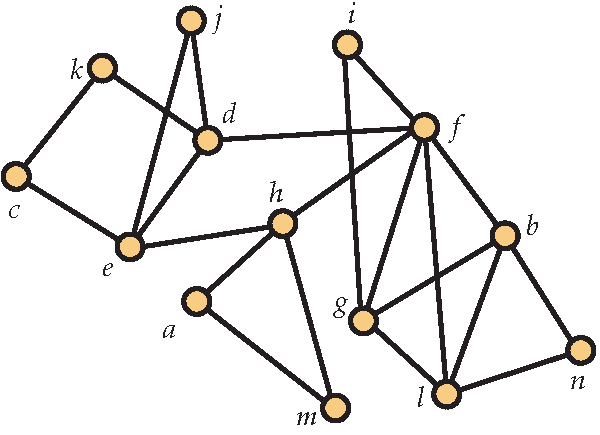
\includegraphics[scale=0.6]{graphs-figs/coloring_ex}
    \caption{A graph $\bfG$ to color}
    \label{fig:graphs:coloring_ex}
  \end{figure}
\item A pharmaceutical manufacturer is building a new warehouse to
  store its supply of $10$ chemicals it uses in production. However,
  some of the chemicals cannot be stored in the same room due to undesirable
  reactions that will occur. The matrix below has a $1$ in position
  $(i,j)$ if and only if chemical $i$ and chemical $j$ cannot be
  stored in the same room. Develop an appropriate graph theoretic
  model and determine the smallest number of rooms into which they can
  divide their warehouse so that they can safely store all $10$
  chemicals in the warehouse.
  \[
  \begin{bmatrix}
    0 & 1 & 0 & 1 & 1 & 0 & 1 & 0 & 0 & 0\\
    1 & 0 & 0 & 1 & 1 & 0 & 0 & 0 & 0 & 1\\
    0 & 0 & 0 & 0 & 0 & 1 & 0 & 1 & 1 & 0\\
    1 & 1 & 0 & 0 & 1 & 0 & 0 & 0 & 0 & 0\\
    1 & 1 & 0 & 1 & 0 & 0 & 0 & 0 & 1 & 0\\
    0 & 0 & 1 & 0 & 0 & 0 & 1 & 0 & 0 & 1\\
    1 & 0 & 0 & 0 & 0 & 1 & 0 & 1 & 0 & 0\\
    0 & 0 & 1 & 0 & 0 & 0 & 1 & 0 & 0 & 0\\
    0 & 0 & 1 & 0 & 1 & 0 & 0 & 0 & 0 & 0\\
    0 & 1 & 0 & 0 & 0 & 1 & 0 & 0 & 0 & 0
  \end{bmatrix}
  \]
\item A school is preparing the schedule of classes for the next
  academic year. They are concerned about scheduling calculus,
  physics, English, statistics, economics, chemistry, and German
  classes, planning to offer a single section of each one. Below are
  the lists of courses that each of six students must take in order to
  successfully graduate. Determine the smallest number of class
  periods that can be used to schedule these courses if each student
  can take at most one course per class period. Explain why fewer
  class periods cannot be used.
  \begin{center}
    \begin{tabular}{c|l}
      Student & Courses\\\hline
      1 & Chemistry, Physics, Economics\\
      2 & English, German, Statistics\\
      3 & Statistics, Calculus, German\\
      4 & Chemistry, Physics\\
      5 & English, Chemistry\\
      6 & Chemistry, Economics
    \end{tabular}
  \end{center}
\item All trees with more than one vertex have the same chromatic
  number. What is it, and why?
\item \label{ex:color} Find a proper $(t+1)$-coloring of the
  graph $\bfG_{t+1}$ in Mycielski's proof of
  \hyperref[prop:triangle-free]{Proposition~\ref*{prop:triangle-free}}. This
  establishes that $\chi(\bfG_{t+1})\leq t+1$.
\item How many vertices does the graph $\bfG_4$ from the Kelly and
  Kelly proof of
  \hyperref[prop:triangle-free]{Proposition~\ref*{prop:triangle-free}}
  have?
\item Construct and draw the graph $\bfG_5$ from Mycielski's proof of
  \hyperref[prop:triangle-free]{Proposition~\ref*{prop:triangle-free}}.
\item Find a recursive formula for the number of vertices $n_t$ in the
  graph $\bfG_t$ from the Kelly and Kelly proof of
  \hyperref[prop:triangle-free]{Proposition~\ref*{prop:triangle-free}}.
\item Let $b_t$ be the number of vertices in the graph $\bfG_t$ from
  the Mycielski's proof of
  \hyperref[prop:triangle-free]{Proposition~\ref*{prop:triangle-free}}. Find
  a recursive formula for $b_t$.
\item The \emph{girth} of a graph $\bfG$ is the number of vertices in
  a shortest cycle of $\bfG$. Find the girth of the graph $\bfG_t$ in
  the Kelly and Kelly proof of
  \hyperref[prop:triangle-free]{Proposition~\ref*{prop:triangle-free}}
  and prove that your answer is correct. As a challenge, see if you
  can modify the construction of $\bfG_t$ to increase the girth. If
  so, how far are you able to increase it?
\item \label{ex:graphs:first-fit-color}Use the First Fit algorithm to
  color the graph in \autoref{fig:k44minus} using the two different
  orderings of the vertex set shown there.
\item Draw the interval graph corresponding to the intervals in
  \autoref{fig:graphs:intervals-ex}.
  \begin{figure}[h]
    \centering
    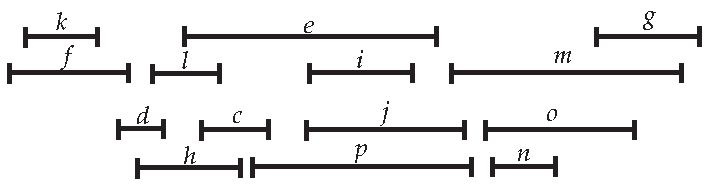
\includegraphics{graphs-figs/firstfit-intgraph}
    \caption{A collection of intervals}
    \label{fig:graphs:intervals-ex}
  \end{figure}
\item Use the First Fit coloring algorithm to find the chromatic
  number of the interval graph whose interval representation is shown
  in \autoref{fig:graphs:intervals-ex} as well as a proper coloring
  using as few colors as possible.
\item 
  \begin{enumerate}
   \item From
    \hyperref[ex:graphs:first-fit-color]{exercise~\ref*{ex:graphs:first-fit-color}}
    you know that choosing a bad ordering of the vertices of a graph
    can lead to the First Fit coloring algorithm producing a coloring
    that is far from optimal. However, you can use this algorithm to
    prove a bound on the chromatic number. Show that if every vertex
    of $\bfG$ has degree at most $D$, then $\chi(\bfG)\leq D+1$.
  \item Give an example of a bipartite graph with $D=1000$ to show
    that this bound need not be tight.
  \end{enumerate}
\item Is the graph in \autoref{fig:graphs:coloring_ex} planar? If it
  is, find a drawing without edges crossings. If it is not give a reason why it is
  not.
\item Is the graph in \autoref{fig:graphs:planar_ex} planar? If it
  is, find a drawing without edge crossings. If it is not give a reason why it is
  not.
  \begin{figure}[h]
    \centering
    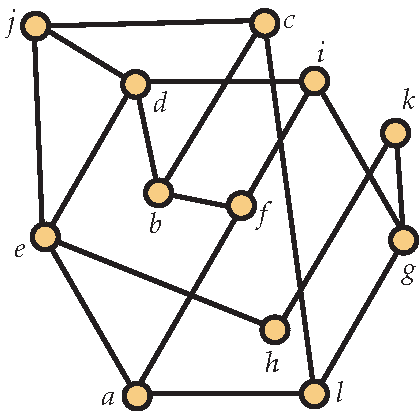
\includegraphics[scale=0.6]{graphs-figs/planar_ex}
    \caption{Is this graph planar?}
    \label{fig:graphs:planar_ex}
  \end{figure}

\item Find a planar drawing of the graph $\bfK_5-e$, by which we mean
  the graph formed from the complete graph on $5$ vertices by deleting
  any edge.
\item Draw a planar drawing of an eulerian planar graph with $10$
  vertices and $21$ edges.
\item Show that every planar graph has a vertex that is incident to at
  most five edges.
\item \label{ex:graphs:degseq}Let $\GVE$ be a graph with $V=\{v_1,v_2,\dots,v_n\}$. Its
  \emph{degree sequence} is the list of the degrees of its vertices,
  arranged in nonincreasing order. That is, the degree sequence of
  $\mathbf{G}$ is
  $(\deg_\mathbf{G}(v_1),\deg_\mathbf{G}(v_2),\dots,\deg_\mathbf{G}(v_n))$
  with the vertices arranged such that $\deg_\mathbf{G}(v_1) \geq
  \deg_\mathbf{G}(v_2)\geq \cdots\geq \deg_\mathbf{G}(v_n)$. Below
  are five sequences of integers (along with $n$, the number of
  integers in the sequence). Identify
  \begin{itemize}
  \item the \textit{one} sequence that \textbf{cannot be the degree
      sequence of any graph};
  \item the \textit{two} sequences that could be the degree sequence
    of a \textbf{planar} graph;
  \item the \textit{one} sequence that could be the degree sequence of
    a \textbf{tree};
  \item the \textit{one} sequence that is the degree sequence of
    an \textbf{eulerian} graph; and
  \item the \textit{one} sequence that is the degree sequence of a
    graph that must be \textbf{hamiltonian}.
  \end{itemize}
  Explain your answers. (Note that one sequence will get two labels
  from above.)
  \begin{enumerate}
  \item $n=10$: $(4,4,2,2,1,1,1,1,1,1)$
  \item $n=9$: $(8,8,8,6,4,4,4,4,4)$
  \item $n=7$: $(5,4,4,3,2,1,0)$
  \item $n=10$: $(7,7,6,6,6,6,5,5,5,5)$
  \item $n=6$: $(5,4,3,2,2,2)$
  \end{enumerate}
\item \label{ex:graphs:degseq2} Below are three sequences of length $10$. One of the sequences
  cannot be the degree sequence (see
  \hyperref[ex:graphs:degseq]{exercise~\ref*{ex:graphs:degseq}}) of
  any graph. Identify it and say why. For each of the other two, say
  \emph{why} (if you have enough information) a \emph{connected} graph
  with that degree sequence
  \begin{itemize}
  \item is definitely hamiltonian/cannot be hamiltonian;
  \item is definitely eulerian/cannot be eulerian;
  \item is definitely a tree/cannot be a tree; and
  \item is definitely planar/cannot be planar.
  \end{itemize}
  (If you do not have enough information to make a determination for a
  sequence without having specific graph(s) with that degree sequence,
  write ``not enough information'' for that property.) 
  \begin{enumerate}
  \item $(6,6,4,4,4,4,2,2,2,2)$
  \item $(7,7,7,7,6,6,6,2,1,1)$
  \item $(8,6,4,4,4,3,2,2,1,1)$
  \end{enumerate}
\item For the two degree sequences in
  \hyperref[ex:graphs:degseq2]{exercise~\ref*{ex:graphs:degseq2}} that
  correspond to graphs, there were some properties for which the
  degree sequence was not sufficient information to determine if the
  graph had that property. For each of those situations, see if you
  can draw both a graph that has the property and a graph that does
  not have the property.
\item Draw the $16$ labeled trees on $4$ vertices.
\item Determine $\prufer(\bfT)$ for the tree $\bfT$ in \autoref{fig:graphs:tree-10verts-ex1}.
  \begin{figure}[h]
    \begin{center}
      \begin{overpic}{graphs-figs/tree-10verts-ex1}
        \put(35,11.2){$1$}
        \put(46,2){$2$}
        \put(22,25){$3$}
        \put(22,9){$4$}
        \put(68,2.5){$5$}
        \put(90,11){$6$}
        \put(5,16){$7$}
        \put(77,21){$8$}
        \put(62,14.5){$9$}
        \put(0.5,2){$10$}
      \end{overpic}
      \caption{A $10$-vertex tree}\label{fig:graphs:tree-10verts-ex1}
    \end{center}
  \end{figure}
\item Determine $\prufer(\bfT)$ for the tree $\bfT$ in \autoref{fig:graphs:tree-10verts-ex2}.
  \begin{figure}[h]
    \begin{center}
      \begin{overpic}{graphs-figs/tree-8verts-ex2}
        \put(50,32){$1$}
        \put(44,2){$2$}
        \put(26,22){$3$}
        \put(31,48){$4$}
        \put(62,56){$5$}
        \put(94,32){$6$}
        \put(5,16){$7$}
        \put(77,21){$8$}
      \end{overpic}
      \caption{A $10$-vertex tree}\label{fig:graphs:tree-10verts-ex2}
    \end{center}
  \end{figure}
\item Determine $\prufer(\bfT)$ for the tree $\bfT$ \autoref{fig:graphs:tree-14verts-ex3}.
  \begin{figure}[h]
    \begin{center}
      \begin{overpic}{graphs-figs/tree-14verts-ex3}
        \put(50,32){$1$}
        \put(44,2){$2$}
        \put(2,34){$3$}
        \put(31,48){$4$}
        \put(62,56){$5$}
        \put(77,21){$6$}
        \put(17,51){$7$}
        \put(94,32){$8$}
        \put(34,20){$9$}
        \put(5,16){$10$}
        \put(74,2){$11$}
        \put(44,9){$12$}
        \put(87,14){$13$}
        \put(64,14){$14$}
    \end{overpic}
    \caption{A $14$-vertex tree}\label{fig:graphs:tree-14verts-ex3}
  \end{center}
\end{figure}
\item Construct the labeled tree $\bfT$ with Pr\"ufer code $96113473$.
\item Construct the labeled tree $\bfT$ with Pr\"ufer code $23134$.
\item Construct the labeled tree $\bfT$ with Pr\"ufer code (using
  commas to separate symbols in the string, since we have labels
  greater than $9$) $10,1,7,4,3,4,10,2,2,8$.
\item (Challenge problem) When $\GVE$ is a graph, let $\Delta(\bfG)$ denote the maximum
  degree in $\bfG$.  Prove \textbf{Brooks' Theorem}:  If $\bfG$ is connected and
  $\Delta(\bfG)=k$, then
  $\chi(\bfG)\le k+1$.  Furthermore, equality holds if and only if
  (a)~$k=2$ and $\bfG$ is an odd cycle, or (b)~$k\neq2$ and $\bfG=\bfK_{k+1}$.
  Hint: It's clear that $\chi(\bfG)\le k+1$ (in fact, this was
  already assigned as an exercise). Assume that $\chi(\bfG)=k+1$
  but that neither conclusion (a) or (b) holds.  Take a spanning tree of
  $\bfG$ and an appropriate ordering of the
  vertices, with two leaves of the tree coming first.  Then show that a 
  First Fit coloring of the graph will only use $k$ colors.
\end{enumerate}


%%% Local Variables: 
%%% mode: latex
%%% TeX-master: "chap-skel-mtk"
%%% End: 

% posets.tex
% updated January 11, 2012

\chapter{Partially Ordered Sets}\label{ch:posets}

Alice was surfing the web and found a site listing top movies, grouped
by categories (comedy, drama, family, etc) as well as by the decade in 
which they were released.  Alice was intrigued by the critic's choices
and his rankings, especially for the top seven dramas from the 1990's.
Alice agreed with the critic's choices as a group but not the
specific rankings.  She wrote the critic's rankings on the board
and just to the right, she gave her own rankings, all the time
insisting that she was certainly correct in her opinions.


\begin{center}
\begin{minipage}{.45\textwidth}
\noindent
\textbf{Movie Critic's Ranking}

\begin{enumerate}
\item Saving Private Ryan 
\item Life is Beautiful 
\item Forrest Gump
\item Braveheart
\item Good Will Hunting
\item Titanic
\item Jurassic Park
\end{enumerate}
\end{minipage}
\begin{minipage}{.45\textwidth}
\noindent
\textbf{Alice's Ranking}

\begin{enumerate}
\item Life is Beautiful 
\item Saving Private Ryan 
\item Good Will Hunting
\item Titanic
\item Braveheart
\item Forrest Gump
\item Jurassic Park
\end{enumerate}
\end{minipage}
\end{center}

Dave studied the two rankings and listened carefully to Alice's rationale
(which he felt was a bit over the top), but eventually, he held up the following
diagram and offered it as a statement of those comparisons on which both Alice
and the movie critic were in agreement. 

\begin{figure}
\begin{center}
\includegraphics*[scale=.4]{posets-figs/movies.pdf}
\caption{Top Movies from the 90's}
\label{fig:movies}
\end{center}
\end{figure}

\begin{remark}
Do you see how Dave made up this diagram?  Add your own rankings of these
seven films and then draw the diagram that Dave would produce as a statement
about the comparisons on which you, Alice and the movie critic were in agreement.
\end{remark}

More generally, when humans are asked to express preferences among 
a set of options, they often report that establishing a totally ranked list 
is difficult if not impossible.  Instead, they prefer to report a partial 
order---where comparisons are made between certain pairs of options but not 
between others.  In this chapter, we
make these observations more concrete by introducing the concept of 
a partially ordered set.  Elementary examples include (1)~a family of sets which is 
partially ordered by inclusion and (2)~a set of positive integers which is
partially ordered by division.  From an applications standpoint, a
complex construction job typically involves a large number of projects
for which there is a notion of precedence between some but not all pairs.
Also, computer file systems are modeled by trees which become partially 
ordered sets whenever links are added.

\section{Basic Notation and Terminology}\label{s:posets:intro}

A \textit{partially ordered set} or \textit{poset} $\bfP$ is a pair
$(X,P)$ where $X$ is a set and $P$ is a reflexive, antisymmetric, and
transitive binary relation on $X$. (Refer to \autoref{s:background:order} for a
refresher of what these properties are if you need to.) We call $X$
the \textit{ground set} while $P$ is a \textit{partial order} on
$X$. Elements of the ground set $X$ are also called \textit{points},
and the poset $\bfP$ is \textit{finite} if its ground set $X$ is a
finite set.

\begin{example}\label{exa:binaryrel}
Let $X=\{a,b,c,d,e,f\}$ and consider the following binary relations
on $X$.
\begin{enumerate}
\item $R_1=\{(a,a),(b,b),(c,c),(d,d),(e,e),(f,f),(a,b),(a,c),(e,f)\}$.
\item $R_2=\{(a,a),(b,b),(c,c),(d,d),(e,e),(f,f),(d,b),(d,e),(b,a),(e,a),$\\
 $(d,a),(d,e),(c,f)\}$.
\item $R_3=\{(a,a),(b,b),(c,c),(d,d),(e,e),(f,f),(a,c),(a,e),(a,f),(b,c),$\\
 $(b,d),(b,e),(b,f),(d,e),(d,f),(e,f)\}$.
\item $R_4=\{(a,a),(b,b),(c,c),(d,d),(e,e),(f,f),(d,b),(b,a),(e,a),(c,f)\}$.
\item $R_5=\{(a,a),(c,c),(d,d),(e,e),(a,e),(c,a),(c,e),(d,e)\}$.
\item $R_6=\{(a,a),(b,b),(c,c),(d,d),(e,e),(f,f),(d,f),(b,e),(c,a),(e,b)\}$.
\end{enumerate}
Then $R_1$, $R_2$ and $R_3$ are partial orders on $X$, so $\bfP_1=(X,R_1)$,
$\bfP_2=(X,R_2)$ and $\bfP_3=(X,R_3)$ are posets.  Several of the other examples
we will discuss in this chapter will use the poset $\bfP_3=(X,R_3)$.  

On the other hand, $R_4$, $R_5$ and $R_6$ are not partial orders on
$X$.  Note that $R_4$ is not transitive, as it contains $(d,b)$ and
$(b,a)$ but not $(d,a)$.  The relation $R_5$ is not reflexive, since
it doesn't contain $(b,b)$.  (Also, it also doesn't contain $(f,f)$,
but one shortcoming is enough.) Note that $R_5$ is a partial order on
$\{a,b,d,e\}$.  The relation $R_6$ is not antisymmetric, as it
contains both $(b,e)$ and $(e,b)$.
\end{example}

When $\PXP$ is a poset, it is common to write $x\le y$ in $P$ and
$y\ge x$ in $P$ as substitutes for $(x,y)\in P$. Of course, the notations $x<y$ in
$P$ and $y>x$ in $P$ mean $x\le y$ in $P$ and $x\ne y$.  When the
poset $\bfP$ remains fixed throughout a discussion, we will sometimes
abbreviate $x\le y$ in $P$ by just writing $x\le y$, etc.  When $x$
and $y$ are distinct points from $X$, we say $x$ is \textit{covered}
by $y$ in $P$\footnote{Reflecting the vagaries of the English
  language, mathematicians use the phrases: (1) $x$ is covered by $y$
  in $P$; (2)~$y$ covers $x$ in $P$; and (3)~$(x,y)$ is a cover in $P$
  interchangeably.}  when $x<y$ in $P$, and there is no point $z\in X$
for which $x<z$ an $z<y$ in $P$.  For example, in the poset
$\bfP_3=(X,R_3)$ from
\hyperref[exa:binaryrel]{Example~\ref*{exa:binaryrel}}, $d$ is covered
by $e$ and $c$ covers $b$. However, $a$ is not covered by $f$, since
$a<e<f$ in $R_3$.  We can then associate with the poset $\bfP$ a
\textit{cover graph} $\mathbf{G}$ whose vertex set is the ground set
$X$ of $\bfP$ with $xy$ an edge in $\mathbf{G}$ if and only if one of
$x$ and $y$ covers the other in $\bfP$.  Again, for the poset $\bfP_3$
from \hyperref[exa:binaryrel]{Example~\ref*{exa:binaryrel}}, we show
the cover graph on the left side of \autoref{fig:covergraphs}.
Actually, on the right side of this figure is just another drawing of
this same graph.

\begin{figure}
\begin{center}
\includegraphics*[scale=.4]{posets-figs/covergraphs.pdf}
\caption{Cover Graph}
\label{fig:covergraphs}
\end{center}
\end{figure}

It is convenient to illustrate a poset with a suitably drawn diagram
of the cover graph in the Euclidean plane.  We choose a standard
horizontal/vertical coordinate system in the plane and require that
the vertical coordinate of the point corresponding to $y$ be larger
than the vertical coordinate of the point corresponding to $x$
whenever $y$ covers $x$ in $P$. Each edge in the cover graph is
represented by a straight line segment which contains no point
corresponding to any element in the poset other than those associated
with its two end points.  Such diagrams are called \textit{Hasse
  diagrams} (\textit{poset diagrams, order diagrams}, or just
\textit{diagrams}).  Now it should be clear that the drawing on the
right side of \autoref{fig:covergraphs} is a diagram of the poset
$\bfP_3$ from \hyperref[exa:binaryrel]{Example~\ref*{exa:binaryrel}},
while the diagram on the left is not.

For posets of moderate size, diagrams are frequently used to define a poset---rather
than the explicit binary relation notation illustrated in \hyperref[exa:binaryrel]{Example~\ref*{exa:binaryrel}}.
In \autoref{fig:17ptposet}, we illustrate a poset $\PXP$ with ground set 
$X=[17]=\{1,2,\dots,17\}$.  It would take several lines of text to write out the
binary relation $P$, and somehow the diagram serves to give us a more tactile sense
of the properties of the poset. 

\begin{figure}
\begin{center}
\includegraphics*[scale=.4]{posets-figs/17ptposet.pdf}
\caption{A Poset on 17 Points}
\label{fig:17ptposet}
\end{center}
\end{figure}

\begin{remark}
Alice and Bob are talking about how you communicate with
a computer in working with posets.  Bob says that computers
have incredible graphics capabilities these days and that you
just give the computer a pdf scan of a diagram.  Alice says
that she doubts that anybody really does that.  Carlos says
that there are several effective strategies.  One way is to label 
the points with positive integers from $[n]$ where $n$ is the 
number of points in the ground set and then define a $0$--$1$
$n\times n$ matrix $A$ with entry $a(i,j)=1$ when $i\le j$ in $P$
and $a(i,j)=0$ otherwise.  Alternatively, you can just provide
for each element $i$ in the ground set a vector $U(x)$ listing all
elements which are greater than $x$ in $P$.  This vector can
be what computer scientists call a \textit{linked list}.
\end{remark}
 
\begin{example}\label{exa:construct}
There are several quite natural ways to construct posets.
\begin{enumerate}
\item A family $\mathcal{F}$ of sets is partially ordered by
inclusion, i.e., set $A\le B$ if and only if $A$ is a subset of
$B$.  
\item A set $X$ of positive integers is partially ordered by
division---without remainder, i.e., set $m\le n$ if and only if
$n\equiv 0\pmod{m}$.  
\item A set $X$ of $t$-tuples of real numbers is
partially ordered by the rule: \\
$(a_1,a_2,\dots,a_t)\le (b_1,b_2,\dots,b_t)$ if
and only if $a_i\le b_i$ in the natural order on $\reals$ for $i=1,2,\dots,t$.
\item When $L_1$, $L_2,\dots,L_k$ are linear orders on the same set
$X$, we can define a partial order $P$ on  $X$ by setting
$x\le y$ in $P$ if and only if $x\le y$ in $L_i$ for all $i=1,2,\dots,k$.
\end{enumerate}
We illustrate the first three constructions with the posets shown in 
\autoref{fig:constructposets}.  As is now clear, in the discussion at the 
very beginning of this chapter, Dave drew a diagram for the poset determined by 
the intersection of the linear orders given by Alice and the movie critic.
\end{example}

\begin{figure}
\begin{center}
\includegraphics*[scale=.4]{posets-figs/constructposets.pdf}
\caption{Constructing Posets}
\label{fig:constructposets}
\end{center}
\end{figure}

Distinct points $x$ and $y$ in a poset $\PXP$ are \textit{comparable}
if either $x<y$ in $P$ or $x>y$ in $P$; otherwise $x$ and $y$ are
\textit{incomparable}.  With a poset $\PXP$, we associate a 
\textit{comparability} graph ${\bfG}_1=(X,E_1)$ and an 
\textit{incomparability} graph ${\bfG}_2=(X,E_2)$. The edges in the 
comparability graph ${\bfG}_1$ consist of the comparable pairs and 
the edges in the incomparability graph are the incomparable pairs.  We 
illustrate these definitions in \autoref{fig:compincomp}
where we show the comparability graph and the incomparability graph
of the poset $\bfP_3$.

\begin{figure}
\begin{center}
\includegraphics*[scale=.4]{posets-figs/compincomp.pdf}
\caption{Comparability and Incommparability Graphs}
\label{fig:compincomp}
\end{center}
\end{figure}

A partial order $P$ is called a \textit{total} order (also, a 
\textit{linear} order) if for all $x,y\in X$, either $x\le y$ in $P$
or $y\le x$ in $P$.  For small finite sets, we can specify a linear
order by listing the elements from least to greatest.  For example,
$L=[b,c,d,a,f,g,e]$ is the linear order on the ground set $\{a,b,c,d,e,f,g\}$ with
$b<c<d<a<f<g<e$ in $L$.   

The set of real numbers comes equipped with a natural total order.  For example,
$1<7/5<\sqrt{2}<\pi$ in this order.  But in this chapter, we will be interested
primarily with partial orders that are \textit{not} linear orders.  Also, we note
that special care must be taken when discussing partial orders on ground sets
whose elements are real numbers.  For the poset shown in \autoref{fig:17ptposet}, note
that $14$ is less than $8$, while $3$ and $6$ are incomparable.
Best not to tell your parents that you've learned that under certain circumstances,
$14$ can be less than $8$ and that you may be able to say which of $3$ and $6$ is 
larger than the other.  The subtlety may be lost in the heated 
discussion certain to follow.

When $\PXP$ is a poset and $Y\subseteq X$, the binary relation
$Q=P\cap(Y\times Y)$ is a partial order on $Y$, and we call the
poset $(Y,Q)$ a \textit{subposet} of $\bfP$.  In \autoref{fig:subposet},
we show a subposet of the poset first presented in \autoref{fig:17ptposet}.

\begin{figure}
\begin{center}
\includegraphics*[scale=.4]{posets-figs/subposet.pdf}
\caption{A Subposet}
\label{fig:subposet}
\end{center}
\end{figure}

When $\PXP$ is a poset and $C$ is a subset of $X$,
we say that $C$ is a \textit{chain} if every distinct pair of points 
from $C$ is comparable in $P$.  When $P$ is a linear order, the entire ground 
set $X$ is a chain.  Dually, if $A$ is a subset of $X$, we say that
$A$ is an \textit{antichain} if every distinct pair of points from $A$ 
is incomparable in $P$.  Note that a one-element subset
is both a chain and an antichain.  Also, we consider the emptyset as
both a chain and an antichain.

The \textit{height} of a poset
$(X,P)$, denoted $\height(P)$, is the largest $h$ for which there exists
a chain of $h$ points in $P$.
Dually, the \textit{width} of a poset $\PXP$, denoted $\width(P)$, is the
largest $w$ for which there exists an antichain of $w$ points in
$P$. 

\begin{remark}
Given a poset $\PXP$, how hard is to determine its height and width?
Bob says that it is very easy.  For example, to find the width of a poset, just 
list all the subsets of $X$.  Delete those which are not antichains.
The answer is the size of the largest subset that remains.  He is quick
to assert that the same approach will work to find the height.
Alice groans at Bob's naivety and suggests that he should read
further in this chapter.
\end{remark}

\section{Additional Concepts for Posets}\label{s:posets:additional-concepts}

We say $(X,P)$ and $(Y,Q)$ are \textit{isomorphic}, and write $(X,P)
\cong(Y,Q)$ if there exists a bijection (1--1 and
onto map) $f:X\to Y$ so that $x_1\le x_2$ in $P$ if and only if
$f(x_1)\le f(x_2)$ in $Q$. In this definition, the map $f$ is called an
\textit{isomorphism} from $\bfP$ to $\bfQ$.  In \autoref{fig:constructposets},
the first two posets are isomorphic.

\begin{remark}  Bob sees a pattern linking the first two posets
shown in \autoref{fig:constructposets} and asserts that any poset of one of these
two types is isomorphic to a poset of the other type.  Alice admits that Bob
is right---but even more is true.  The four constructions given in 
Example~\ref{exa:construct} are universal in the sense that \textit{every}
poset is isomorphic to a poset of each of the four types.  Do you see why? 
If you get stuck answering this, we will revisit the question at the
end of the chapter, and we will give you a hint.
\end{remark}

An isomorphism from $\bfP$ to 
$\bfP$ is called an \textit{automorphism} of $\bfP$. An isomorphism from 
$\bfP$ to a subposet of $\bfQ$ is called an \textit{embedding} of
$\bfP$ in $\bfQ$. In most settings, we will not distinguish between
isomorphic posets, and we will say that a poset $\PXP$ is \textit{contained}
in $\QYQ$ (also $\bfQ$ \textit{contains} $\bfP$) when there is an
embedding of $\bfP$ in $\bfQ$. Also, we will say that $\bfP$ \textit{excludes}
$\bfQ$ when no subposet of $\bfP$ is isomorphic to $\bfQ$, and we will 
frequently say $\bfP=\bfQ$ when $\bfP$ and $\bfQ$ are isomorphic.

With the notion of isomorphism, we are lead naturally to the notion of
an ``unlabelled'' posets, and in \autoref{f:unlabelled}, we show a
diagram for such a poset.

\begin{figure}[hb]
\begin{center}
\includegraphics*[scale=.4]{posets-figs/wttfig-5.pdf}
\caption{\label{f:unlabelled}An Unlabelled Partially Ordered Set}
\end{center}
\end{figure}

\begin{remark}
How hard is it to tell whether two posets are isomorphic?  Bob thinks
it's not too difficult.  Bob says that if you give him a bijection between
the ground sets, then he can quickly determine whether you have
established that the two posets are isomorphic.  Alice senses that
Bob is confusing the issue of testing whether two posets are isomorphic
with simply verifying that a particular bijection can be certified to
be an isomorphism.  The first problem seems much harder to her. Carlos says that he
thinks it's actually very hard and that in fact, no one knows whether there is
a good algorithm.  
\end{remark}

Note that the poset shown in \autoref{f:unlabelled} has the property
that there is only one maximal point.  Such a point is sometimes
called a \textit{one}, denoted not surprisingly as~$1$.  Also, there
is only one minimal point, and it is called a \textit{zero},
denoted~$0$.

The \textit{dual} of a partial order $P$ on a set $X$ is denoted by
$P^d$ and is defined by $P^d=\{(y,x):(x,y)\in P\}$. The \textit{dual}
of the poset $\PXP$ is denoted by $\bfP^d$ and is defined by
$\bfP^d=(X,P^d)$. A poset $\bfP$ is \textit{self-dual} if
$\bfP=\bfP^d$.

A poset $\PXP$ is \textit{connected} if its comparability graph is 
connected, i.e., for every $x,y\in X$ with
$x\ne y$, there is a finite sequence $x=x_0,x_1,\dots,x_n=y$ of points
from $X$ so that $x_i$ is comparable to $x_{i+1}$ in $P$ for
$i=0,1,2,\dots,n-1$. A subposet $(Y,P(Y))$ of $(X,P)$ is called a
\textit{component} of $\bfP$ if $(Y,P(Y))$ is connected and there is
no subset $Z\subseteq X$ containing $Y$ as a proper subset for which
$(Z,P(Z))$ is connected.  A one-point component is \textit{trivial}
(also, a \textit{loose} point or \textit{isolated} point); components
of two or more points are \textit{nontrivial}.  Note that a loose
point is both a minimal element and a maximal element.  Returning to
the poset shown in \autoref{fig:17ptposet}, we see that it has two
components.

It is natural to say that a graph $\bfG$ is a \emph{comparability graph}
when there is a poset $\PXP$ whose comparability graph is isomorphic
to $\bfG$.  For example, we show in \autoref{fig:noncompgraph} a graph on
$6$ vertices which is not a comparability graph. (We leave the task of
establishing this claim as an exercise.)

\begin{figure}
\begin{center}
\includegraphics*[scale=.4]{posets-figs/noncompgraph.pdf}
\caption{\label{fig:noncompgraph}A Graph Which is Not a Comparability Graph}
\end{center}
\end{figure}

Similarly, we say that a graph $\bfG$ is a \emph{cover graph} when there
exists a poset $\PXP$ whose cover graph is isomorphic to $\bfG$.  Not
every graph is a cover graph.  In particular, any graph which contains
a triangle is not a cover graph.  In the exercises at the end of the
chapter, you will be asked to construct triangle-free graphs which are
not cover graphs---with some hints given as to how to proceed.

\begin{remark} Bob is quite taken with graphs associated with posets.  He makes the
following claims.

\begin{enumerate}
\item Only linear orders have paths as cover graphs.
\item A poset and its dual have the same cover graph and the
same comparability graph.  
\item Any two posets with the same cover graph have the same
height and the same width.
\item Any two posets with the same comparability graph have the
same height and the same width.
\end{enumerate}
Alice shrugs and says that Bob is right half the time.  Which two assertions
are correct?

Undeterred, Bob notes that the comparability graph shown in \autoref{fig:compincomp}
is also an incomparability graph (for another poset).  He goes on to posit that
this is always true, i.e., whenever $\bfG$ is the comparability graph of
a poset $\bfP$, there is another poset $\bfQ$ for which $\bfG$ is the incomparability
graph of $\bfQ$.  Alice says that Bob is right on the first count but she is
not so sure about the second.  Dave mumbles that they should take a look at
the comparability graph of the third poset in \autoref{fig:constructposets}.  This
graph is not an incomparability graph.  But in his typical befuddled manner,
Dave doesn't offer any justification for this statement.  Can you help Alice
and Bob to see why Dave is correct?

Bob is on a roll and he goes on to suggest that it is relatively easy to 
determine whether a graph is a comparability graph (he read it on the web), but he has a 
sense that determining whether a graph is a cover graph might be difficult.  
Do you think he is right---on
either count?  
\end{remark}

\section{Dilworth's Chain Covering Theorem and its Dual}\label{s:posets:dilworth}

In this section, we prove the following theorem of R. P. Dilworth,
which is truly one of the classic results of combinatorial mathematics.

\begin{theorem}[Dilworth's Theorem]\label{thm:dilworth}
If $\PXP$ is a poset and $\width(P)=w$, then there exists a 
partition $X=C_1\cup C_2\cup\dots \cup C_w$, where $C_i$ is a 
chain for $i=1,2,\dots,w$. Furthermore, there is no chain partition
into fewer chains.
\end{theorem}

Before proceeding with the proof of Dilworth's theorem, we pause to
discuss the dual version for partitions into antichains, as it is
even easier to prove.

\begin{theorem}\label{thm:dualdilworth}
If $\PXP$ is a poset and $\height(P)=h$,
then there exists a partition $X=A_1\cup A_2\cup\dots\cup A_h$, where
$A_i$ is an antichain for $i=1,2,\dots,h$. Furthermore, there is no
partition using fewer antichains.
\end{theorem}

\begin{proof}
For each $x\in X$, let $\height(x)$ be the largest integer $t$ for
which there exists a chain \[x_1<x_2<\dots < x_t\] with $x=x_t$.
Evidently, $\height(x)\le h$ for all $x\in X$.  Then for each
$i=1,2,\dots,h$, let $A_i=\{x\in X:\height(x)=i\}$.  It is easy to
see that each $A_i$ is an antichain, as if $x,y\in A_i$ are such
that $x<y$, then there is a chain $x_1<x_2<\cdots<x_i=x <
x_{i+i}=y$, so $\height(y)\ge i+1$. Since $\height(P)=h$, there is a
maximum chain $C=\{x_1,x_2,\dots,x_h\}$. If it were possible to
partition $\bfP$ into $t<h$ antichains, then by the pigeonhole
principle, one of the antichains would contain two points from $C$,
but this is not possible.
\end{proof}

When $\PXP$ is a poset, a point $x\in X$ with $\height(x)=1$ is 
called a \textit{minimal} point of $\bfP$.  We denote the set of all minimal
points of a poset $\PXP$ by $\min(X,P)$ \footnote{Since we use the
notation $\bfP= (X,P)$ for a poset, the set of minimal elements can
be denoted by $ \min(\bfP)$ or $\min(X,P)$. This convention will be
used for all set valued and integer valued functions of posets.}.

The argument given for the proof of \autoref{thm:dualdilworth} yields
an efficient algorithm, one that is defined recursively.  Set $\bfP_0=
\bfP$.  If $\bfP_i$ has been defined and $\bfP_i\neq \emptyset$, let
$A_i=\min(\bfP_i)$ and then let $\bfP_{i+1}$ denote the subposet remaining
when $A_i$ is removed from $\bfP_i$.

In \autoref{fig:height5}, we illustrate the antichain partition
provided by this algorithm for the $17$ point poset from \autoref{fig:17ptposet}.  
The darkened points form a chain of size~$5$. 

\begin{figure}
\begin{center}
\includegraphics*[scale=.4]{posets-figs/height5}
\caption{A Poset of Height 5}
\label{fig:height5}
\end{center}
\end{figure}

\begin{remark}
Alice claims that it is very easy to find the set of minimal elements of
a poset.  Do you agree?
\end{remark}

Dually, we can speak of the set $\max(\bfP)$ of \textit{maximal} points
of $\bfP$.  We can also partition $\bfP$ into $\height(\bfP)$ antichains
by recursively removing the set of maximal points.

We pause to remark that when $\PXP$ is a poset, the set of all chains of
$\bfP$ is itself partially ordered by inclusion.  So it is natural to
say that a chain $C$ is \textit{maximal} when there is no chain
$C'$ containing $C$ as a proper subset.  Also, a chain $C$ is \textit{maximum}
when there is no chain $C'$ with $|C|<|C'|$.  Of course, a maximum chain
is maximal, but maximal chains need not be maximum.

Maximal antichains and maximum antichains are defined analogously.

With this terminology, the thrust of \autoref{thm:dualdilworth} is
that it is easy to find the height $h$ of a poset as well as a maximum
chain $C$ consisting of $h$ points from $\bfP$.  Of course, we also get
a handy partition of the poset into $h$ antichains.

\subsection{Proof of Dilworth's Theorem}

The argument for Dilworth's theorem is simplified by the 
following notation. When $\PXP$ is a poset and $x\in X$, we let $D(x)=\{y\in 
X:y<x \text{ in }P\}$; $D[x]=\{y\in X:y\le x\text{ in }P\}$; $U(x)=\{y\in X:y>x
\text{ in }P\}$; $U[x]=\{y\in X:y\ge x\}$; and $I(x)=\{y\in X-\{x\}:x\Vert y
\text{ in }P\}$. When $S\subseteq  X$, we let $D(S)=
\{y\in X:y<x$ in $P$, for some $x\in S\}$ and $D[S]=S\cup D(S)$. The
subsets $U(S)$ and $U[S]$ are defined dually.  Note that when 
$A$ is a maximal antichain in $\bfP$, the ground set $X$ can be
partitioned into pairwise disjoint sets as $X=A\cup D(A)\cup U(A)$.

We are now ready for the proof.  Let $\PXP$ be a poset and let $w$ denote
the width of $\bfP$.
As in~\autoref{thm:dualdilworth}, the pigeonhole principle implies
that we require at least $w$ chains in any chain partition of
$\bfP$. To prove that $w$ suffice, we
proceed by induction on $|X|$, the result being trivial if
$|X|=1$. Assume validity for all posets with $|X|\le k$ and suppose
that $\PXP$ is a poset with $|X|=k+1$. Without loss of generality,
$w>1$; else the trivial partition $X=C_1$ satisfies the
conclusion of the theorem. Furthermore, we observe that if $C$ is a
(nonempty) chain in $(X,P)$, then we may assume that the subposet
$(X-C,P(X-C))$ also has width $w$. To see this, observe that the
theorem holds for the subposet, so that if
$\width(X-C,P(X-C))=w'<w$, then we can partition $X-C$ as
$X-C=C_1\cup C_2\cup\dots\cup C_{w'}$, so that $X=C\cup
C_1\cup\dots\cup C_{w'}$ is a partition into $w'+1$ chains. Since
$w'<w$, we know $w'+1\le w$, so we have a partition of $X$ into at
most $w$ chains. Since any partition of $X$ into chains must use at
least $w$ chains, this is exactly the partition we seek.

Choose a maximal point $x$ and a minimal point $y$ with $y\le x$ in
$P$. Then let $C$ be the chain containing only the points $x$ and $y$. Note that
$C$ contains either one or two elements depending on whether $x$
and $y$ are distinct.

Let $Y=X-C$ and  $Q=P(Y)$ and let $A$ be a $w$-element antichain
in the  subposet $(Y,Q)$.  In the partition $X=A\cup D(A)\cup U(A)$, the
fact that $y$ is a minimal point while $A$ is a maximal
antichain imply that $y\in D(A)$.  Similarly, $x\in U(A)$.  In particular,
this shows that $x$ and $y$ are distinct.

Label the elements of $A$ as
$\{a_1,a_2,\dots,a_w\}$. Note
that $U[A]\ne X$ since $y\notin U[A]$, and $D[A]\ne X$ since
$x\notin D[A]$. Therefore, we may apply the inductive hypothesis to
the suposets of $\bfP$ determined by $D[A]$ and $U[A]$, respectively,
and partition each of these two subposets into $w$ chains: 

\[
U[A]= C_1\cup C_2\cup\dots\cup C_w\quad\text{and}\quad
 D[A]=D_1\cup D_2\cup\dots\cup D_w
\]
Without loss of generality, we may assume these chains have
been labeled so that $a_i\in C_i\cap D_i$ for each $i=1,2,\dots,w$. 
However, this implies that 
\[
X=(C_1\cup D_1)\cup (C_2\cup D_2)\cup\dots\cup(C_w\cup D_w)
\]
is the desired partition which in turn completes the proof.

In \autoref{fig:width7}, we illustrate Dilworth's chain covering
theorem for the poset first introduced in \autoref{fig:17ptposet}.
The darkened points form a $7$-element antichain, while the labels
provide a partition into~$7$ chains.

\begin{figure}
\begin{center}
\includegraphics*[scale=.4]{posets-figs/width7.pdf}
\caption{A Poset of Width 7}
\label{fig:width7}
\end{center}
\end{figure}

\begin{remark}
The ever alert Alice notes that
the proof given above for Dilworth's theorem does not seem to provide
an efficient algorithm for finding the width~$w$ of a poset, much less
a partition of the poset into $w$ chains.  Bob has yet to figure out
why listing all the subsets of $X$ is a bad idea.  Carlos is sitting
quietly listening to their bickering, but finally, he says that a skilled
programmer can devise an algorithm from the proof.  Students are encouraged
to discuss this dilemma---but rest assured that we will return to 
this issue later in the text.
\end{remark}

\section{Linear Extensions of Partially Ordered Sets}\label{s:posets:sorting}

Let $\PXP$ be a partially ordered set.  A linear order $L$ on $X$ is
called a \textit{linear extension} (also, a \textit{topological sort})
of $P$, if $x<y$ in $L$ whenever $x<y$ in $P$.  For example, the
table displayed in \autoref{fig:posets:lin-extn} shows that our familiar
example $\bfP_3$ has~11 linear extensions.

\begin{figure}
\begin{center}
\begin{minipage}{.25\textwidth}
\begin{overpic}[scale=.4]{posets-figs/wttfig-9}
\put(-3,2){$z$}
\put(48,32.5){$w$}
\put(48,2){$a$}
\put(-3,32.5){$b$}
\put(48,63){$c$}
\put(48,93){$d$}
\end{overpic}\hspace{.5in}
\end{minipage}
\begin{minipage}{.70\textwidth}
\[
\begin{array}{ccccccccccc}
L_1& L_2 & L_3 & L_4 & L_5 & L_6 & L_7 & L_8 & L_9 & L_{10} & L_{11}\\[.2in]
% \vspace{.2in}
 d & d & d & b & d & d & d & b & d & d & b \\
 c & c & b & d & c & c & b & d & c & b & d \\
 w & b & c & c & w & b & c & c & b & c & c \\
 b & w & w & w & b & w & w & w & z & z & z \\
 a & a & a & a & z & z & z & z & w & w & w \\
 z & z & z & z & a & a & a & a & a & a & a \\
\end{array}
\]
\end{minipage}
\caption{\label{fig:posets:lin-extn}A poset and its linear extensions}
\end{center}
\end{figure}

\begin{remark}
Bob says that he is not convinced that every finite poset has a linear
extension.  Alice says that it is easy to show that they do.  Is she right?

Carlos says that there are subtleties to this question when the ground
set $X$ is infinite.  You might want to do a web search on the name Szpilrajn and 
read about his contribution to this issue.
\end{remark}

The classical sorting problem studied in all elementary computer
science courses is to determine an unknown linear order $L$ of a set $X$
by asking a series of questions of the form:\quad Is $x<y$ in $L$?
All the well known sorting algorithms (bubble sort,
merge sort, quick sort, etc.) proceed in this manner.

Here is an important special case: determine an unknown linear 
extension $L$ of a poset $\bfP$ by asking a series of questions of the form:
\quad Is $x < y$ in $L$?  

\begin{remark}
Given the poset $\PXP$ shown in \autoref{fig:17ptposet} and the problem of 
determining an unknown linear extension of $P$, how should Alice decide 
which question (of the form:\quad Is $x<y$ in $L$?) to ask?  

How would you like to be assigned to count the
number of linear extensions of this poset?  In general, 
how hard is it to determine the number of linear extensions of a poset?
Could you (and your computer) do this count for a poset on $100,000$ points?
\end{remark}

\section{The Subset Lattice}\label{s:posets:subset-lattice}

When $X$ is a finite set, the family of all subsets of $X$, partially
ordered by inclusion, forms a
\textit{subset lattice\footnote{A lattice is a special type of
    poset. You do not have to concern yourself with the definition and
    can safely replace ``lattice'' with ``poset'' as you read this
    chapter.}}.  We illustrate this in \autoref{fig:4cube} where we
show the lattice of all subsets of $\{1,2,3,4\}$. In this figure, note
that we are representing sets by bit strings, and we have further
abbreviated the notation by writing strings without commas and
parentheses.

\begin{figure}
\begin{center}
\includegraphics*[scale=.4]{posets-figs/4cube.pdf}
\caption{A Subset Lattice}
\label{fig:4cube}
\end{center}
\end{figure}

For a positive integer $t$, we let $\bftwo^t$ denote the subset
lattice consisting of all subsets of $\{1,2,\dots,t\}$
ordered by inclusion.  Some elementary properties of this
poset are:

\begin{enumerate}
\item The height is $t+1$ and all maximal chains have exactly
$t+1$ points.
\item The size of the poset $\bftwo^t$ is $2^t$ and the elements
are partitioned into ranks (antichains) $A_0, A_1,\dots, A_t$
with $|A_i|=\binom{t}{i}$ for each $i=0,1,\dots,t$.
\item The maximum size of a rank in the subset lattice occurs
in the middle, i.e. if $s=\lfloor t/2\rfloor$, then the
largest binomial coefficient in the sequence $\binom{t}{0},
\binom{t}{1},\binom{t}{2},\dots,\binom{t}{t}$ is $\binom{t}{s}$.
Note that when $t$ is odd, there are two ranks of maximum size,
but when $t$ is even, there is only one.
\end{enumerate}

\subsection{Sperner's Theorem}\label{ss:posets:subset-lattice:sperner}

For the width of the subset lattice, we have the following
classic result due to Sperner.

\begin{theorem}[Sperner]\label{thm:sperner}
For each $t\ge1$, the width of the subset lattice $\bftwo^t$
is the maximum size of a rank, i.e., 
\[
\width(\bftwo^t)=\binom{t}{\lfloor\frac{t}{2}\rfloor}
\]
\end{theorem}

\begin{proof}
The width of the poset $\bftwo^t$ is at least
$C(t,\lfloor\frac{t}{2}\rfloor)$ since the set of all
$\lfloor\frac{t}{2}\rfloor$-element subsets of $\{1,2,\dots,t\}$ is an
antichain.  We now show that the width of $\bftwo^t$ is at most
$C(t,\lfloor\frac{t}{2}\rfloor)$.

Let $w$ be the width of $\bftwo^t$ and let $\{S_1,S_2,\dots, S_w\}$ be
an antichain of size $w$ in this poset, i.e., each $S_i$ is a subset
of $\{1,2,\dots,t\}$ and if $1\le i<j\le w$, then $S_i\nsubseteq
S_j$ and $S_j\nsubseteq S_i$.

For each $i$, consider the set $\cgS_i$ of all maximal chains which
pass through $S_i$.  It is easy to see that if $|S_i|=k_i$, then
$|\cgS_i|=k_i!(t-k_i)!$.  This follows from the observation that to
form such a maximum chain beginning with $S_i$ as an intermediate
point, you delete the elements of $S_i$ one at a time to form the
sets of the lower part of the chain.  Also, to form the upper part
of the chain, you add the elements not in $S_i$ one at a time.

Note further that if $1\le i <j\le w$, then $\cgS_i\cap \cgS_j
=\emptyset$, for if there was a maximum chain belonging to both
$\cgS_i$ and $\cgS_j$, then it would imply that one of $S_i$ and
$S_j$ is a subset of the other.

Altogether, there are exactly $t!$ maximum chains in $\bftwo^t$.  This
implies that
\[\sum_{i=1}^{w} k_i!(t-k_i)!\le t!.\]
This implies that
\[\sum_{i=1}^{w}\frac{k_i!(t-k_i)!}{t!}=
\sum_{i=1}^{w}\frac{1}{\binom{t}{k_i}}\le 1. 
\]
It follows that
\[
\sum_{i=1}^{i=w}\frac{1}{\binom{t}{\lceil\frac{t}{2}\rceil}}\le 1
\]
Thus
\[
w\le \binom{t}{\lceil\frac{t}{2}\rceil}.
\]
\end{proof}

\section{Interval Orders}\label{s:posets:intervalorder}

When we discussed Dilworth's theorem, we commented that the
algorithmic aspects would be deferred until later in the text.  But
there is one important class of orders for which the full solution is
easy to obtain.

A poset $\PXP$ is called an \textit{interval order} if there exists a
function $I$ assigning to each element $x\in X$ a closed interval
$I(x)=[a_x,b_x]$ of the real line $\reals$ so that for all $x$, $y\in
X$, $x<y$ in $P$ if and only if $b_x<a_y$ in $\reals$.  We call $I$ an
\textit{interval representation} of $\bfP$, or just a
\textit{representation} for short.  For brevity, whenever we say that
$I$ is a representation of an interval order $\PXP$, we will use the
alternate notation $[a_x,b_x]$ for the closed interval $I(x)$.  Also,
we let $|I(x)|$ denote the \textit{length} of the interval, i.e.,
$|I(x)|=b_x-a_x$.  Returning to the poset $\bfP_3$, the representation
shown in \autoref{fig:6ptintorder} shows that it is an interval order.

\begin{figure}
\begin{center}
\includegraphics*[scale=.4]{posets-figs/6ptintorder.pdf}
\caption{An interval order and its representation}
\label{fig:6ptintorder} 
\end{center}
\end{figure}

Note that end points of intervals used in a representation need not be
distinct.  In fact, distinct points $x$ and $y$ from $X$ may satisfy
$I(x)=I(y)$.  We even allow degenerate intervals, i.e., those of the
form $[a,a]$.  On the other hand, a representation is said to be
\textit{distinguishing} if all intervals are non-degenerate and all
end points are distinct. It is relatively easy to see that every interval order
has a distinguishing representation.

\begin{theorem}[Fishburn]\label{thm:fishburn}
Let $\PXP$ be a poset.  Then $\bfP$ is an interval order if 
and only if it excludes $\bftwo+\bftwo$.
\end{theorem}

\begin{proof}
We show only that an interval order cannot contain a subposet
isomorphic to $\bftwo+\bftwo$, deferring the proof in the other 
direction to the next section.  Now suppose that $\PXP$ is a poset,
$\{x,y,z,w\}\subseteq X$ and the subposet
determined by these four points is isomorphic to $\bftwo+\bftwo$.
We show that $\bfP$ is not an interval order.  Suppose to the
contrary that $I$  is an interval representation of $\bfP$.  Without loss 
of generality, we may assume that $x<y$ and $z<w$ in $P$.  Thus $x\Vert w$ and
$z\Vert y$ in $P$.  Then $b_x<a_y$ and $b_z < a_w$ in $\reals$ 
so that $a_w \le b_x <a_y \le b_z$, which is a contradiction.

\end{proof}

\section{Finding a Representation of an Interval Order}
\label{s:posets:intervalorder:findrep}

In this section, we develop an algorithm for finding an interval
representation of an interval order.  In fact, this
algorithm can be applied to any poset.  Either it will find
an interval representation or it will find a subposet isomorphic
to $\bftwo+\bftwo$.  As a consequence, we establish the other half of Fishburn's theorem.

When $\PXP$ is an interval order and $n$ is a positive integer, there
may be many different ways to represent $\bfP$ using intervals with
integer end points in $[n]$.  But there is certainly a least $n$ for
which a representation can be found, and here  we see that the representation is
unique.  The discussion will again make use of the notation for down
sets and up sets that we introduced prior to the proof of Dilworth's
Theorem. As a reminder, we repeat it here. For a poset $\PXP$ and a
subset $S\subset X$, let $D(S) = \{y\in X:$ there exists some $x\in S$
with $y<x$ in $P\}$.  Also, let $D[S]=D(S)\cup S$.  When $|S|=1$, say
$S=\{x\}$, we write $D(x)$ and $D[x]$ rather than $D(\{x\})$ and
$D[\{x\}]$.  Dually, for a subset $S\subseteq X$, we define $U(S) =
\{y\in X:$ there exists some $x\in X$ with $y>x$ in $P\}$.  As before,
set $U[S]=U(S)\cup S$.  And when $S=\{x\}$, we just write $U(x)$ for
$\{y\in X:x<y$ in $P\}$.

Let $\PXP$ be a poset.  We start our procedure by finding
the following subsets of the ground set:\quad  
$\mathcal{D} = \{D(x):x\in X\}$.  We then distinguish two
cases.  In the first case, there are distinct elements
$x$ and $y$ for which $D(x)\nsubseteq D(y)$ and $D(y)\nsubseteq D(x)$.
In this case, we choose an element $z\in D(x)-D(y)$ and an element
$w\in D(y)-D(x)$.  It follows that the four elements in
$\{x,y,z,w\}$ form a subposet of $\bfP$ which is isomorphic to
$\bftwo+\bftwo$. 

Our second case is that either $D(x)\subseteq D(y)$ or
$D(y)\subseteq D(x)$ for all $x,y\in X$.  In this case, we
will show that $\bfP$ is an interval order.  Now find
the family: $\mathcal{U} = \{U(x):x\in X\}$.  In this case, it is 
easy to see that we will always have either $U(x)\subseteq U(y)$ or
$U(y)\subseteq U(x)$ for all $x,y\in X$.

Let $d=|\mathcal{D}|$.  In the exercises, we will provide
(actually in doing your homework, \textit{you} will provide) the details
for backing up the following statement:
$|\mathcal{U}|=|\mathcal{D}|$, so for now we assume that this
statement is valid.
Label the sets in $\mathcal{D}$ and $\mathcal{U}$ respectively as
$D_1$, $D_2,\dots,D_d$ and $U_1$, $U_2,\dots,U_d$ 
so that
\[
\emptyset= D_1\subset D_2\subset D_3\subset\dots\subset D_d
 \quad\text{and}
\]
\[
U_1\supset U_{2}\cdots \supset U_{d-2}\supset U_{d-1}\supset\dots\supset U_d
 =\emptyset.
\]
We form an interval representation $I$ of $\bfP$ by the
following rule:  For each $x\in X$, set $I(x)=[i,j]$, where
$D(x)=D_i$ and $U(x)=U_j$.  It is not immediately clear that this
rule is legal, i.e., it might happen that applying the rule results
in values of $i$ and $j$ for which $j<i$.  But again, as a result of
the exercises, we will see that this never happens. This collection
of exercises is summarized in the following theorem.

\begin{theorem}\label{thm:intord-minrep}
Let $\bfP$ be a poset excluding $\bftwo+\bftwo$.
then 
\begin{enumerate}
\item $|\mathcal{D}|=|\mathcal{U}|$.
\item For each $x\in X$, if $I(x)=[i,j]$, then $i\le j$ in $\mathbb{R}$.
\item For each $x,y\in X$, if $I(x)=[i,j]$ and $I(y)=[k,l]$, then
$x<y$ in $P$ if and only if $j<k$ in $\mathbb{R}$.
\item The integer $d$ is the least positive integer for which
$\bfP$ has an interval representation using integer end points
from $[d]$.  This representation is unique.
\end{enumerate}
\end{theorem}

Consider the poset shown in \autoref{fig:10ptintorder}.

\begin{figure}
\begin{center}
\includegraphics*[scale=.4]{posets-figs/10ptintorder.pdf}
\caption{An interval order on 10 Points}
\label{fig:10ptintorder} 
\end{center}
\end{figure}

Then $d= 5$ with 
$D_1=\emptyset$, $D_2=\{c\}$, $D_3=\{c,f,g\}$, $D_4=\{c,f,g,h\}$, and 
$D_5=\{a,c,f,g,h,j\}$.  Also
$U_1=\{a,b,d,e,h,i,j\}$, $U_2=\{a,b,e,h,i,j\}$,
$U_3=\{b,e,i\}$, $U_4=\{e\}$, and $U_5=\emptyset$.
So
\begin{align*}
I(a) &= [3,4]\\
I(b) &= [4,5]\\
I(c) &= [1,1]\\
I(d) &= [2,5]\\
I(e) &= [5,5]\\
I(f) &= [1,2]\\
I(g) &= [1,2]\\
I(h) &= [3,3]\\
I(i) &= [4,5]\\
I(j) &= [3,4]
\end{align*}

To illustrate the situation where this process can be used to
determine when a poset is not an interval order, consider again the
poset shown in Figure.  Erase the line joining points $c$ and $d$.
For the resulting poset,  you will then find that $D(j)=\{f,g\}$
and $D(d)=\{c\}$.  Therefore, the four points $c$, $d$, $f$ and $j$
form a copy of $\bftwo+\bftwo$ in this modified poset.

\section{Dilworth's Theorem for Interval Orders}\label{s:posets:dilworth-intord}

As remarked previously, we do not yet have an efficient
process for determining the width of a poset and a minimum
partition into chains.  For interval orders, there is indeed
a simple way to find both. The explanation is just to establish
a connection with coloring of interval graphs as discussed in
\autoref{ch:graphs}.

Let $\PXP$ be an interval order and let 
$\{[a_x,b_x]:x\in X\}$ be intervals of the real line
so that $x<y$ in $\bfP$ if and only $b_x<a_y$.
Then let $\bfG$ be the interval graph determined by this
family of intervals.  Note that if $x$ and $y$ are distinct
elements of $X$, then $x$ and $y$ are incomparable in $\bfP$ if and
only if $xy$ is an edge in $\bfG$.  In other words, $\bfG$ is
just the incomparability graph of $\bfP$.

Recall from Chapter~$4$ that interval graphs are perfect, i.e.,
$\chi(\bfG)=\omega(\bfG)$ for every interval graph $\bfG$.  Furthermore,
you can find an optimal coloring of an interval graph by applying first fit
to the vertices in a linear order that respects left end points.
Such a coloring concurrently determines a partition of $\bfP$ into
chains.

In fact, if you want to skip the part about interval representations,
take any linear ordering of the elements as $x_1$, $x_2,\dots,x_n$ so that
$i<j$ whenever $D(x)$ is a proper subset of $D(y)$.  Then apply First
Fit with respect to chains.  For example, using
the $10$ point interval order illustrated in \autoref{fig:10ptintorder},
here is such a labeling: 

\[\begin{array}{ccccc}
x_1 =g &
x_2 =f &
x_3 =c &
x_4 =d &
x_5 =h\\
x_6 =a &
x_7 =j &
x_8 =b &
x_9 =i &
x_{10} =e
\end{array}\]
Now apply the \textbf{First Fit} algorithm to the points of $\bfP$,
in this order, to assign them to chains $C_1$, $C_2,\dots$.  In other
words, assign $x_1$ to chain~$C_1$.  Thereafter if you have
assigned points $x_1$, $x_2,\dots,x_i$ to chains, then assign
$x_{i+1}$ to chain $C_j$ where $j$ is the least positive integer
for which $x_{i+1}$ is comparable to $x_k$ whenever $1\le k\le i$ and
$x_k$ has already been assigned to $C_j$.
For example, this rule results in the following chains for the
interval order $\bfP$ shown in \autoref{fig:10ptintorder}.

\begin{align*}
C_1 &= \{g,h,b\}\\ 
C_2 &= \{f,a,e\}\\
C_3 &= \{c,d\}\\
C_4 &= \{j\}\\
C_5 &= \{i\}
\end{align*}
In this case, it is easy to see that the chain partition is
optimal since the width of $\bfP$ is $5$ and $A=\{a,b,d,i,j\}$
is a $5$-element antichain.

However, you should be very careful in applying First Fit to find
optimal chain partitions of posets---just as one must be leary of
using First Fit to find optimal colorings of graphs.

\begin{example}
  The poset on the left side of \autoref{fig:FirstFit} is a height~$2$
  poset on $10$ points, and if the poset is partitioned into
  antichains by applying First Fit and considering the points in the
  order of their labels, then $5$ antichains will be used.  Do you see
  how to extend this poset to force First Fit to use arbitrarily many
  antichains, while keeping the height of the poset at $2$?

  On the right side, we show a poset of width~$2$.  Now if this poset
  is partitioned into chains by applying First Fit and considering the
  points in the order of their labels, then $4$ chains will be used.
  Do you see how to extend this poset to force First Fit to use
  arbitrarily many chains while keeping the width of the poset at $2$?

  Do you get a feeling for why the second problem is a bit harder than
  the first?
\end{example}

\begin{figure}
\begin{center}
\includegraphics*[scale=.4]{posets-figs/FirstFit.pdf}
\caption{How First Fit Can Go Wrong}
\label{fig:FirstFit} 
\end{center}
\end{figure}

In general, there is always \textit{some} linear order on the ground set 
of a poset for which First Fit will find an optimal partition into antichains.  
Also, there is a linear order (in general different from the first) on the ground 
set for which First Fit will find an optimal partition into chains.
However, there is no advantage in searching for such orders, as the algorithms
we develop for finding optimal antichain and chain partitions work quite well.

\section{Discussion}\label{s:posets:discussion}

Over coffee, Bob said that he really liked this chapter.  ``This
material was full of cases of very concrete procedures for doing
useful things.  I like that.''  Yolanda offered a somewhat different
perspective ``On the other hand, this last procedure only seems
to work with interval orders and we still don't have a clue as to
how to find the width of a poset in the general case.  This might
be very difficult---like the graph coloring problems discussed in
the last chapter.''  Dave weighed in with ``Somehow I think there's
going to be a fairly efficient process that works for all posets.
We may not have all the tools yet, but let's wait a bit.''

Not much was said for a while and after a pause, Carlos ventured
that there were probably a lot of combinatorial problems for
posets that had analogous versions for graphs and in those cases,
the poset version would be a bit more complicated, sometime a little
bit and sometimes a very big bit.
Zori was quiet but she was thinking.  These poset structures might
even be useful, as she could imagine many settings in which a
linear order was impossible or impractical.  Maybe there were ways
here to earn a few dollars.

\section{Exercises}\label{s:posets:exercises}

\begin{enumerate}
\item We say that a relation $R$ on a set $X$ is \textit{symmetric} if
  $(x,y)\in R$ implies $(y,x)\in R$ for all $x,y\in X$. If
  $X=\{a,b,c,d,e,f\}$, how many symmetric relations are there on $X$?
  How many of these are reflexive?
\item A relation $R$ on a set $X$ is an \textit{equivalence relation}
  if $R$ is reflexive, symmetric, and transitive. Fix an integer
  $m\geq 2$. Show that the relation defined on the set
  $\ints$ of integers by $aRb$ ($a,b\in\ints$) if and only if $a\equiv
  b\pmod{m}$ is an equivalence relation. (Recall that $a\equiv
  b\pmod{m}$ means that when dividing $a$ by $m$ and $b$ by $m$ you
  get the same remainder.)
\item Is the binary relation \[P=\{(1,1),(2,2),(3,3),(4,4),(1,3),(2,4),(2,5),(4,5),(3,5),(1,5)\}\] a partial
  order on the set $X=\{1,2,3,4,5\}$? If so, discuss what properties
  you verified and how. If not, list the ordered pairs that must be
  added to $P$ to make it a partial order or say why it cannot be made
  a partial order by adding ordered pairs.
\item Draw the diagram of the poset $\bfP=(X,P)$ where
  $X=\{1,2,3,5,6,10,15,30\}$ and $x\leq y$ in $P$ if and only if
  $x|y$. (Recall that $x|y$ means that $x$ evenly divides $y$ without
  remainder. Equivalently $x|y$, if and only if $y\equiv
  0\pmod{x}$.) \label{exer:posets:division}
\item Draw the diagram of the poset $\PXP$ where
 \begin{multline*}
    X=\{\{1,3,4,5,6\},\{1,2,4,5,6\},\{1,2,3,6\},\{1,2,3\},\{1,5,6\},\\\{1,3,6\},\{1,2\},\{1,6\},\{3,5\},\{1\},\{3\},\{4\}\}
  \end{multline*}
 and $P$ is the partial order on $X$ given by the ``is a subset of''
 relationship.
\item A \textit{linear extension} of a poset $\bfP=(X,P)$ is a total
  order $L$ on $X$ such that if $x\leq y$ in $P$, then $x\leq y$ in $L$. Give 
  linear extension of the three posets shown in \autoref{fig:constructposets}.
  If you feel very ambitious, try to count the number of linear extensions of
  the poset on the left side of the figure.  Don't list them.  Just provide an
  integer as your answer.
\item Alice and Bob are considering posets $\bfP$ and $\bfQ$. They
  soon realize that $\bfQ$ is isomorphic to $\bfP^d$. After $10$
  minutes of work, they figure out that $\bfP$ has height $5$ and
  width $3$. Bob doesn't want do find the height and width of $\bfQ$,
  since he figures it will take (at least) another $10$ minutes to
  answer these questions for $\bfQ$. Alice says Bob is crazy and that
  she already knows the height and width of $\bfQ$. Who's right and
  why?  
\item For this exercise, consider the poset $\bfP$ in \autoref{fig:17ptposet}.
  \begin{enumerate}
  \item List the maximal elements of $\bfP$.
  \item List the minimal elements of $\bfP$.
  \item Find a maximal chain with two points in $\bfP$.
  \item Find a chain in $\bfP$ with three points that is \emph{not}
    maximal. Say why your chain is not maximal.
  \item Find a maximal antichain with four points in $\bfP$.
  \end{enumerate}
\item Find the height $h$ of the poset $\PXP$ shown below as well as a
  maximum chain and a partition of $X$ into $h$ antichains using the
  algorithm from this chapter.
  \begin{center}
    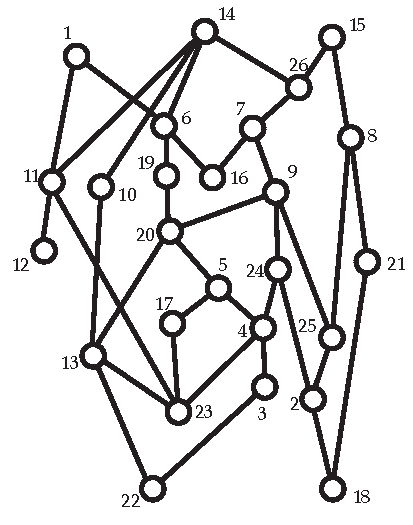
\includegraphics{posets-figs/height_ex_poset}
  \end{center}
\item For each of the two distinct (up to isomorphism) posets in 
  \autoref{fig:constructposets}, find the width $w$, an
  antichain of size $w$, and a partition of the ground set into $w$
  chains.
\item A restaurant chef has designed a new set of dishes for his
  menu. His set of dishes contains $10$ main courses, and he will
  select a subset of them to place on the menu each night. To ensure
  variety of main courses for his patrons, he wants to guarantee that
  a night's menu is neither completely contained in nor completely
  contains another night's menu. What is the largest number of menus
  he can plan using his $10$ main courses subject to this requirement?
\item Draw the diagram of the interval order represented in
  \autoref{fig:intord_to_diag_ex}.
  \begin{figure}[h]
  \begin{center}
    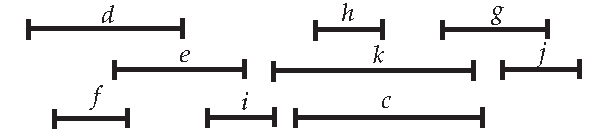
\includegraphics{posets-figs/intord_to_diag_ex}
  \end{center}
  \caption{An interval representation}\label{fig:intord_to_diag_ex}
  \end{figure}
\item Draw the diagram of the interval order represented in
  \autoref{fig:intord_to_diag_ex2}.
  \begin{figure}[h]
  \begin{center}
    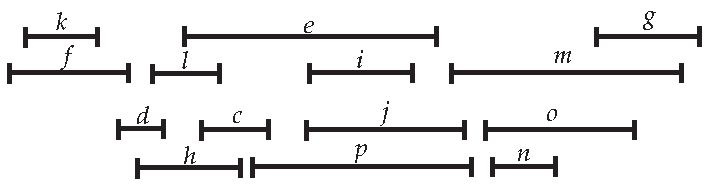
\includegraphics{posets-figs/intord_to_diag_ex2}
  \end{center}
  \caption{An interval representation}\label{fig:intord_to_diag_ex2}
  \end{figure}
\item Find an interval representation for the poset in
  \autoref{fig:intord_find_rep_ex1} or give a reason why one does not
  exist.
  \begin{figure}[h]
  \begin{center}
    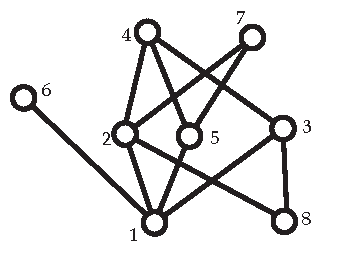
\includegraphics{posets-figs/intord_find_rep_ex1}
  \end{center}
  \caption{Is this poset an interval order?}\label{fig:intord_find_rep_ex1}
  \end{figure}
\item Find an interval representation for the poset in
  \autoref{fig:intord_find_rep_ex4} or give a reason why one does not
  exist.
  \begin{figure}[h]
  \begin{center}
    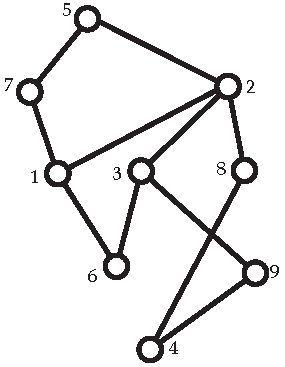
\includegraphics{posets-figs/intord_find_rep_ex4}
  \end{center}
  \caption{Is this poset an interval order?}\label{fig:intord_find_rep_ex4}
  \end{figure}
\item Find an interval representation for the poset in
  \autoref{fig:intord_find_rep_ex2} or give a reason why one does not
  exist.
  \begin{figure}[h]
  \begin{center}
    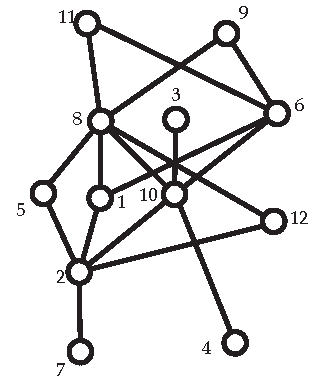
\includegraphics{posets-figs/intord_find_rep_ex2}
  \end{center}
  \caption{Is this poset an interval order?}\label{fig:intord_find_rep_ex2}
  \end{figure}
\item Find an interval representation for the poset in
  \autoref{fig:intord_find_rep_ex3} or give a reason why one does not
  exist.
  \begin{figure}[h]
  \begin{center}
    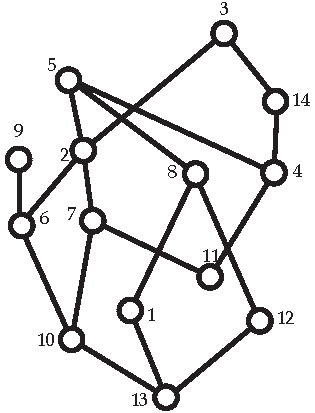
\includegraphics{posets-figs/intord_find_rep_ex3}
  \end{center}
  \caption{Is this poset an interval order?}\label{fig:intord_find_rep_ex3}
  \end{figure}
\item Use the First Fit algorithm (ordering by left endpoints) to find
  the width $w$ of the interval order shown in
  \autoref{fig:intord_firstfit_ex1} and a partition into $w$
  chains. Also give an antichain with $w$ points.
  \begin{figure}[h]
    \centering
    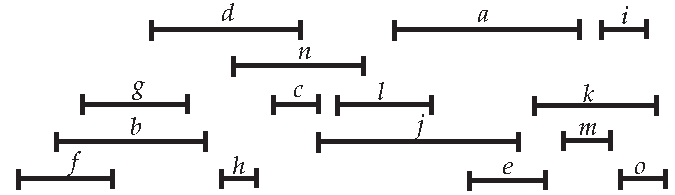
\includegraphics{posets-figs/intord_firstfit_ex1}
    \caption{An interval representation}
    \label{fig:intord_firstfit_ex1}
  \end{figure}
\item Complete the proof of Theorem\ref{thm:intord-minrep}.  \textit{Hint.}
  The key idea is to show that if $d$ is the least positive integer for
  which an interval order $\bfP$ has a representation using end points from
  $\{1,2,\dots,n\}$, then every integer $i$ from this set must be both a left
  end point and a right end point of an interval.
\item Show that every poset is isomorphic to a poset of each of the four types
  illustrated in Example~\ref{exa:construct}.  Hint: for each element $x$, choose
  some unique identifying key which is an element/prime/coordinate/observer.  Then associate
  with $x$ a structure that identifies the keys of elements from $D[x]$. 
\item The \textit{dimension} of a poset $\PXP$, denoted $\dim(\bfP)$, is the least $t$ for 
  which $P$ is the intersection of $t$ linear orders on $X$.
  \begin{enumerate}
   \item Show that the dimension of a poset $\bfP$ is the same as the dimension of its dual.
   \item Show that $\bfP$ is a subposet of $\bfQ$, then $\dim(\bfP)\le \dim(\bfQ)$.
   \item Show that the removal of a point can reduce the dimension by at most~$1$.
   \item Find the dimension of the posets in \autoref{fig:constructposets}.
   \item Use Dilworth's theorem to show that the dimension of a poset is at most its width.
   \item Use the example on the left side of \autoref{fig:FirstFit} to show that
   for every $n\ge2$, there exists a poset $\bfP_n$ on $2n$ points having width and dimension
   equal to $n$.
   \end{enumerate}
\end{enumerate}

%%% Local Variables: 
%%% mode: latex
%%% TeX-master: "book"
%%% End: 

% inclusionexclusion.tex
% Updated January 11, 2012

\chapter{Inclusion-Exclusion}\label{ch:inclusion-exclusion}

In this chapter, we study a classic enumeration technique known as
Inclusion-Exclusion. In its simplest case, it is absolutely intuitive.
Its power rests in the fact that in many situations, we start with an
exponentially large calculation and see it reduce to a manageable
size. We focus on three applications that every student of
combinatorics should know: (1)~counting surjections, (2)~derangements,
and (3)~the Euler $\phi$-function.

\section{Introduction}\label{s:inclusion-exclusion:intro}

We start this chapter with an elementary example.
\begin{example} \label{exa:inclusion-exclusion:students}
  Let $X$ be the set of $63$ students in an applied combinatorics
  course at a large technological university. Suppose there are $47$
  computer science majors and $51$ male students. Also, we know there
  are $45$ male students majoring in computer science. How many
  students in the class are female students not majoring in computer
  science?

  Although the Venn diagrams that you've probably seen drawn many
  times over the years aren't always the best illustrations
  (especially if you try to think with some sort of scale), let's use
  one to get started. In \autoref{fig:venn-app-comb}, we see how the
  groups in the scenario might overlap.
 \begin{figure}[h]
    \centering
    \begin{overpic}{inclusionexclusion-figs/Venn-diagram}
      \put(15,28.5){Males}
%      \put(78,14){Females}
      \put(63,28.5){CS Majors}
      \put(22,8){Non-CS major females}
    \end{overpic}
    \caption{A Venn diagram for an applied combinatorics class}
    \label{fig:venn-app-comb}
  \end{figure}
  Now we can see that we're after the number of students in the white
  rectangle but outside the two shaded ovals, which is the female
  students not majoring in computer science. To compute this, we can
  start by subtracting the number of male students (the blue region)
  from the total number of students in the class and then subtracting
  the number of computer science majors (the yellow region). However,
  we've now subtracted the overlapping region (the male computer
  science majors) \textit{twice}, so we must add that number
  back. Thus, the number of female students in the class who are not
  majoring in computer science is
  \[63 - 51 - 47 + 45 = 10.\]
\end{example}

\begin{example}\label{exa:inclusion-exclusion:int-solns}
  Another type of problem where we can readily see how such a
  technique is applicable is a generalization of the problem of
  enumerating integer solutions of equations. In \autoref{ch:strings},
  we discussed how to count the number of solutions to an equation
  such as
  \[x_1 + x_2 + x_3 + x_4 = 100,\] where $x_1>0$, $x_2, x_3 \geq 0$
  and $2\leq x_4\leq 10$. However, we steered clear of the situation
  where we add the further restriction that $x_3\leq 7$. The previous
  example suggests a way of approaching this modified problem.

  First, let's set up the problem so that the lower bound on each
  variable is of the form $x_i\geq 0$. This leads us
  to the revised problem of enumerating the integer solutions to
  \[x_1' + x_2 + x_3 + x_4' = 97\] with $x_1',x_2,x_3,x_4'\geq 0$,
  $x_3\leq 7$, and $x_4'\leq 8$. (We'll then have $x_1 = x_1'+1$ and
  $x_4 = x_4' + 2$ to get our desired solution.) To count the number
  of integer solutions to this equation with $x_3\leq 7$ and $x_4'\leq
  8$, we must exclude any solution in which $x_3 > 7$ \emph{or} $x_4'
  > 8$. There are $C(92,3)$ solutions with $x_3 > 7$, and the number
  of solutions in which $x_4'>8$ is $C(91,3)$. At this point, it might
  be tempting to just subtract $C(92,3)$ and $C(91,3)$ from
  $C(100,3)$, the total number of solutions with all variables
  nonnegative. However, care is required. If we did that, we would
  eliminate the solutions with both $x_3>7$ \emph{and} $x_4'>8$
  \emph{twice}. To account for this, we notice that there are
  $C(83,3)$ solutions with both $x_3>7$ and $x_4'>8$. If we add this
  number back in after subtracting, we've ensured that the solutions
  with both $x_3>7$ and $x_4'>8$ are not included in the total count
  and are not excluded more than once. Thus, the total number of
  solutions is 
  \[\binom{100}{3} - \binom{92}{3} - \binom{91}{3} + \binom{83}{3} = 6516.\]
\end{example}

From these examples, you should start to see a pattern emerging that
leads to a more general setting. In full generality, we will consider
a set $X$ and a family $\mathcal{P}=\{P_1,P_2,\dots,P_m\}$ of
\textit{properties}.  We intend that for every $x\in X$ and each
$i=1,2,\dots,m$, either $x$ satisfies $P_i$ or it does not.  There is
no ambiguity.  Ultimately, we are interested in determining the number
of elements of $X$ which satisfy \textit{none} of the properties in
$\mathcal{P}$. In
\hyperref[exa:inclusion-exclusion:students]{Example~\ref*{exa:inclusion-exclusion:students}},
we could have made property $P_1$ ``is a computer science major'' and
property $P_2$ ``is male''. Then the number of students satisfying
\emph{neither} $P_1$ nor $P_2$ would be the number of female students
majoring in something other than computer science, exactly the number
we were asked to determine. What would the properties $P_1$ and $P_2$
be for
\hyperref[exa:inclusion-exclusion:int-solns]{Example~\ref*{exa:inclusion-exclusion:int-solns}}?

Let's consider three examples of larger sets of properties. These
properties will come back up during the remainder of the chapter as we
apply inclusion-exclusion to some more involved situations. Recall
that throughout this book, we use the notation $[n]$ for the set
$\{1,2,\dots,n\}$ when $n$ is a positive integer.

\begin{example}\label{exa:inclusion-exclusion:prop-inject}
  Let $m$ and $n$ be fixed positive integers and let $X$ consist of
  all functions from $[n]$ to $[m]$.  Then for each $i=1,2,\dots,m$,
  and each function $f\in X$, we say that $f$ satisfies $P_i$ if there
  is no $j$ so that $f(j)=i$. In other words, $i$ is not in the image
  or output of the function $f$.

  As a specific example, suppose that $n=5$ and $m=3$. Then the
  function given by the table
  \begin{center}
    \begin{tabular}{c|c|c|c|c|c}
      $i$ & 1 & 2 & 3 & 4 & 5\\
      \hline
      $f(i)$ & 2 & 3 & 2 & 2 & 3
    \end{tabular}
  \end{center}
  satisfies $P_1$ but not $P_2$ or $P_3$.
\end{example} 

\begin{example}\label{exa:inclusion-exclusion:prop-derange} 
  Let $m$ be a fixed positive integer and let $X$ consist of all
  bijections from $[m]$ to $[m]$.  Elements of $X$ are called
  \textit{permutations}.  Then for each $i=1,2,\dots,m$, and each
  permutation $\sigma\in X$, we say that $\sigma$ satisfies $P_i$ if
  $\sigma(i)=i$.

  For example, the permutation $\sigma$ of $[5]$ given in by the table
  \begin{center}
    \begin{tabular}{c|c|c|c|c|c}
      $i$ & 1 & 2 & 3 & 4 & 5\\
      \hline
      $\sigma(i)$ & 2 & 4 & 3 & 1 & 5
    \end{tabular}
  \end{center}
  satisfies $P_3$ and $P_5$ and no other $P_i$.
\end{example} 
Note that in the previous example, we could have said that $\sigma$
satisfies property $P_i$ if $\sigma(i)\neq i$.  But remembering that
our goal is to count the number of elements satisfying none of the
properties, we would then be counting the number of permutations
satisfying $\sigma(i)=i$ for each $i=1,2,\dots,n$, and perhaps we
don't need a lot of theory to accomplish this task---the number is
one, of course.

\begin{example}\label{exa:inclusion-exclusion:prop-divis}
  Let $m$ and $n$ be fixed positive integers and let $X=[n]$.  Then
  for each $i=1,2,\dots,m$, and each $j\in X$, we say that $j$
  satisfies $P_i$ if $i$ is a divisor of $j$. Put another way, the
  positive integers that satisfy property $P_i$ are precisely those
  that are multiples of $i$.

  At first this may appear to be the most complicated of the sets of
  properties we've discussed thus far. However, being concrete should
  help clear up any confusion. Suppose that $n=m=15$. Which properties
  does $12$ satisfy? The divisors of $12$ are $1$, $2$, $3$, $4$, $6$,
  and $12$, so $12$ satisfies $P_1$, $P_2$, $P_3$, $P_4$, $P_6$, and
  $P_{12}$. On the other end of the spectrum, notice that $7$
  satisfies only properties $P_1$ and $P_7$, since those are its only
  divisors.
\end{example} 

\section{The Inclusion-Exclusion Formula}\label{s:inclusion-exclusion:statement}

Now that we have an understanding of what we mean by a property, let's
see how we can use this concept to generalize the process we used in
the first two examples of the previous section.

Let $X$ be a set and let $\mathcal{P}=\{P_1,P_2,\dots,P_m\}$ be a
family of properties. Then for each subset $S\subseteq [m]$, let
$N(S)$ denote the number of elements of $X$ which satisfy property
$P_i$ for all $i\in S$.  Note that if $S=\emptyset$, then $N(S)=|X|$,
as every element of $X$ satisfies every property in $S$ (which
contains no actual properties).

Returning for a moment to
\hyperref[exa:inclusion-exclusion:students]{Example~\ref*{exa:inclusion-exclusion:students}}
with $P_1$ being ``is a computer science major'' and $P_2$ being ``is
male,'' we note that $N(\{1\})=47$, since there are $47$ computer
science majors in the class. Also, $N(\{2\})=51$ since $51$ of the
students are male. Finally, $N(\{1,2\})=45$ since there are $45$ male
computer science majors in the class.

In the examples of the previous section, we subtracted off $N(S)$ for
the sets $S$ of size $1$ and then added back $N(S)$ for the set of
properties of size $2$, since we'd subtracted the number of things
with both properties (male computer science majors or solutions with
both $x_3>7$ and $x_4'>8$) twice. Symbolically, we determined that the
number of objects satisfying none of the properties was
\[N(\emptyset) - N(\{1\}) - N(\{2\}) + N(\{1,2\}).\] Suppose that we
had three properties $P_1,P_2$, and $P_3$. How would we count the
number of objects satisfying none of the properties?  As before, we
start by subtracting for each of $P_1$, $P_2$, and $P_3$. Now we have
removed the objects satisfying both $P_1$ and $P_2$ twice, so we must
add back $N(\{1,2\})$. similarly, we must do this for the objects
satisfying both $P_2$ and $P_3$ and both $P_1$ and $P_3$. Now let's
think about the objects satisfying all three properties. They're
counted in $N(\emptyset)$, eliminated \emph{three times} by the
$N(\{i\})$ terms, and added back three times by the $N(\{i,j\})$
terms. Thus, they're still being counted! Thus, we must yet
subtract $N(\{1,2,3\})$ to get the desired number:
\[N(\emptyset) - N(\{1\}) - N(\{2\}) - N(\{3\}) + N(\{1,2\}) +
N(\{2,3\}) + N(\{1,3\}) - N(\{1,2,3\}).\]
We can generalize this as the following theorem:

\begin{theorem}[Principle of Inclusion-Exclusion]\label{thm:inclusion-exclusion}
The number of elements of $X$ which satisfy none of the properties
in $\mathcal{P}$ is given by
\begin{equation}
\sum_{S\subseteq [m]} (-1)^{|S|}N(S).\label{eq:inclusion-exclusion}
\end{equation}
\end{theorem}
\begin{proof}
  We proceed by induction on the number $m$ of properties. If $m=1$,
  then the formula reduces to $N(\emptyset)-N(\{1\})$.  This is
  correct since it says just that the number of elements which do not
  satisfy property $P_1$ is the total number of elements minus the
  number which do satisfy property $P_1$.

  Now assume validity when $m\le k$ for some $k\ge1$ and consider the
  case where $m=k+1$.  Let $X'=\{x\in X: x$ satisfies $P_{k+1}\}$ and
  $X''=X-X'$ (i.e., $X''$ is the set of elements that do not satisfy
  $P_{k+1}$). Also, let $\mathcal{Q}=\{P_1,P_2,\dots,P_k\}$.  Then for
  each subset $S\subseteq [k]$, let $N'(S)$ count the number of
  elements of $X'$ satisfying property $P_i$ for all $i\in S$.  Also,
  let $N''(S)$ count the number of elements of $X''$ satisfying
  property $P_i$ for each $i\in S$.  Note that $N(S)=N'(S)+N''(S)$ for
  every $S\subseteq [k]$.

  Let $X'_0$ denote the set of elements in $X'$ which satisfy none of
  the properties in $\mathcal{Q}$ (in other words, those that satisfy
  only $P_{k+1}$ from $\mathcal{P}$), and let $X''_0$ denote the set
  of elements of $X''$ which satisfy none of the properties in
  $\mathcal{Q}$, and therefore none of the properties in $\mathcal{P}$.

  Now by the inductive hypothesis, we know
  \[
  |X'_0| = \sum_{S\subseteq [k]} (-1)^{|S|}N'(S)\qquad \text{and}\qquad
 |X''_0| = \sum_{S\subseteq [k]} (-1)^{|S|}N''(S).
\]
It follows that
\begin{align*}
|X''_0| &= \sum_{S\subseteq [k]} (-1)^{|S|}N''(S) = \sum_{S\subseteq [k]} (-1)^{|S|}\left(N(S)-N'(S)\right)\\
        &= \sum_{S\subseteq [k]} (-1)^{|S|}N(S)+
           \sum_{S\subseteq [k]} (-1)^{|S|+1}N(S\cup\{k+1\})\\
        &= \sum_{S\subseteq [k+1]} (-1)^{|S|}N(S).
\end{align*}
\end{proof}

\section{Enumerating Surjections}\label{s:inclusion-exclusion:surjections}

As our first example of the power of inclusion-exclusion, consider the
following situation: A grandfather has $15$ distinct lottery tickets
and wants to distribute them to his four grandchildren so that each
child gets at least one ticket. In how many ways can he make such a
distribution? At first, this looks a lot like the problem of
enumerating integers solutions of equations, except here the lottery
tickets are not identical! A ticket bearing the numbers $1$, $3$,
$10$, $23$, $47$, and $50$ will almost surely not pay out the same
amount as one with the numbers $2$, $7$, $10$, $30$, $31$, and $48$,
so who gets which ticket really makes a difference. Hopefully, you
have already recognized that the fact that we're dealing with lottery
tickets and grandchildren isn't so important here. Rather, the
important fact is that we want to distribute distinguishable objects
to distinct entities, which calls for counting functions from one set
(lottery tickets) to another (grandchildren). In our example, we don't
simply want the total number of functions, but instead we want the
number of surjections, so that we can ensure that every grandchild
gets a ticket.

For positive integers $n$ and $m$, let $S(n,m)$ denote the number of
surjections from $[n]$ to $[m]$.  Note that $S(n,m)=0$ when $n<m$.  In
this section, we apply the Inclusion-Exclusion formula to determine a
formula for $S(n,m)$.  We start by setting $X$ to be the set of all
functions from $[n]$ to $[m]$.  Then for each $f\in X$ and each
$i=1,2,\dots,m$, we say that $f$ satisfies property $P_i$ if $i$ is
not in the range of $f$.

\begin{lemma}
  For each subset $S\subseteq [m]$, $N(S)$ depends only on $|S|$.  In
  fact, if $|S|=k$, then
  \[
  N(S)=(m-k)^n.
  \]
\end{lemma}
\begin{proof}
Let $|S|=k$.  Then a
function $f$ satisfying property $P_i$ for each $i\in S$ is
a string of length $n$ from an alphabet consisting of $m-k$ letters.
This shows that \[N(S)=(m-k)^n.\]
\end{proof}

Now the following result follows immediately from this lemma by
applying the Principle of Inclusion-Exclusion, as there are $C(m,k)$
$k$-element subsets of $[m]$.
\begin{theorem}
  The number $S(n,m)$ of surjections from $[n]$ to $[m]$ is given by:
\[
S(n,m) = \sum_{k=0}^m (-1)^k\binom{m}{k}(m-k)^n.
\]
\end{theorem}

For example, 
\begin{align*}
S(5,3) &= \binom{3}{0}(3-0)^5-\binom{3}{1}(3-1)^5+\binom{3}{2}(3-2)^5-\binom{3}{3}(3-3)^5\\
       &= 243 -96+3-0\\
       &= 150.
\end{align*}

Returning to our lottery ticket distribution problem at the start of
the section, we see that there are $S(15,4)=1016542800$ ways for the
grandfather to distribute his $15$ lottery tickets so that each of the
$4$ grandchildren receives at least one ticket.

\section{Derangements}\label{s:inclusion-exclusion:derangements}

Now let's consider a situation where we can make use of the properties
defined in
\hyperref[exa:inclusion-exclusion:prop-derange]{Example~\ref*{exa:inclusion-exclusion:prop-derange}}. Fix a
positive integer $n$ and let $X$ denote the set of all permutations on
$[n]$.  A permutation $\sigma\in X$ is called a \textit{derangement}
if $\sigma(i)\neq i$ for all $i=1,2,\dots,n$. For example, the first
permutation given below is a derangement, while the second is not.
\begin{center}
  \begin{tabular}{c|cccc}
    $i$ & 1 & 2 & 3 & 4\\\hline
    $\sigma(i)$ & 2 & 4 & 1 & 3
  \end{tabular}\hspace{0.3in}
  \begin{tabular}{c|cccc}
    $i$ & 1 & 2 & 3 & 4\\\hline
    $\sigma(i)$ & 2 & 4 & 3 & 1
  \end{tabular}
\end{center}
If we again let $P_i$ be the property that $\sigma(i)=i$, then the
derangements are precisely those permutations which do not satisfy
$P_i$ for any $i=1,2,\dots,n$.

\begin{lemma}
  For each subset $S\subseteq [n]$, $N(S)$ depends only on $|S|$.  In
  fact, if $|S|=k$, then
  \[
  N(S) = (n-k)!
  \]
\end{lemma}

\begin{proof}
  For each $i\in S$, the value $\sigma(i)=i$ is fixed.  The other
  values of $\sigma$ are a permutation among the remaining $n-k$
  positions, and there are $(n-k)!$ of these.
\end{proof}

As before, the principal result of this section follows immediately
from the lemma and the Principle of Inclusion-Exclusion.

\begin{theorem}
For each positive integer $n$, the number $d_n$ of derangements of $[n]$
satisfies
\[
d_n=\sum_{k=0}^n (-1)^k\binom{n}{k}(n-k)!.
\]

\end{theorem}

For example,
\begin{align*}
d_5 & =\binom{5}{0}5!-\binom{5}{1}4!+\binom{5}{2}3!-\binom{5}{3}2!+
   \binom{5}{4}1!-\binom{5}{5}0!\\
    &=120-120+60-20+5-1\\
    &=44.
\end{align*}

It has been traditional to cast the subject of derangements as a
story, called the Hat Check problem. The story belongs to the period
of time when men wore top hats. For a fancy ball, $100$ men check
their top hats with the Hat Check person before entering the ballroom
floor. Later in the evening, the mischeivous hat check person decides
to return hats at random. What is the probability that all $100$ men
receive a hat other than their own? It turns out that the answer is
very close to $1/e$, as the following result shows.

\begin{theorem}
  For a positive integer $n$, let $d_n$ denote the number of
  derangements of $[n]$. Then
  \[
  \lim_{n\rightarrow\infty}\frac{d_n}{n!} = \frac{1}{e}.
  \] 
  Equivalently, the fraction of all permutations of $[n]$ that are
  derangments approaches $1/e$ as $n$ increases.
\end{theorem}

\begin{proof}
It is easy to see that
\begin{align*}
\frac{d_n}{n!} &= \frac{\sum_{k=0}^n (-1)^k\binom{n}{k}(n-k)!}{n!}\\
               &= \sum_{k=0}^n (-1)^k \frac{n!}{k!(n-k)!}\frac{(n-k)!}{n!}\\
               &= \sum_{k=0}^n (-1)^k \frac{1}{k!}.
\end{align*}
Recall from Calculus that the Taylor series expansion of $e^x$ is given
by 
\[
e^x = \sum_{k=0}^{\infty} \frac{x^k}{k!},
\]
and thus the result then follows by substituting $x=-1$.
\end{proof}

Usually we're not as interested in $d_n$ itself as we are in
enumerating permutations with certain restrictions, as the following
example illustrates.

\begin{example}
  Consider the Hat Check problem, but suppose instead of wanting no
  man to leave with his own hat, we are interested in the number of
  ways to distribute the $100$ hats so that precisely $40$ of the men
  leave with their own hats.

  If $40$ men leave with their own hats, then there are $60$ men who
  do not receive their own hats. There are $C(100,60)$ ways to choose
  the $60$ men who will not receive their own hats and $d_{60}$ ways
  to distribute those hats so that no man receives his own. There's
  only one way to distribute the $40$ hats to the men who must receive
  their own hats, meaning that there are
  \begin{align*}
    \binom{100}{60}d_{60} =
    &420788734922281721283274628333913452107738151595140722182899444\\
    &67852500232068048628965153767728913178940196920
    \end{align*}
  such ways to return the hats.
\end{example}

\section{The Euler $\phi$ Function}\label{s:inclusion-exclusion:euler-phi}

After reading the two previous sections, you're probably wondering why
we stated the Principle of Inclusion-Exclusion in such an abstract
way, as in those examples $N(S)$ depended only on the size of $S$ and
not its contents. In this section, we produce an important example
where the value of $N(S)$ \textit{does} depend on $S$.
Nevertheless, we are able to make a reduction to obtain a useful end
result.  In what follows, let $\posints$ denote the set of positive
integers.

For a positive integer $n\ge2$, let 
\[
\phi(n)=|\{m\in \posints: m\le n, \gcd(m,n)=1\}|.
\]
This function is usually called the Euler $\phi$ function or the Euler
totient function and has many connections to number theory. We won't
focus on the number-theoretic aspects here, only being able to compute
$\phi(n)$ efficiently for any $n$.

For example, $\phi(12)=4$ since the only numbers from $\{1,2,\dots,12\}$
that are relatively prime to $12$ are $1$, $5$, $7$ and $11$. As a
second example, $\phi(9)=6$ since $1$, $2$, $4$, $5$, $7$ and $8$ are
relatively prime to $9$.  On the other hand, $\phi(p)=p-1$ when $p$ is 
a prime.  Suppose you were asked to compute $\phi(321974)$.  How
would you proceed?

In \autoref{ch:induction} we discussed a recursive procedure for
determining the greatest common divisor of two integers, and we wrote
a code for accomplishing this task.  Let's assume that we have a
function declared as follows:

\medskip
\noindent
\begin{tt}
int gcd(int m, int n);
\end{tt}

\medskip
\noindent
that returns the greatest common divisor of $m$ and $n$.

Then we can calculate $\phi(n)$ with this code snippet:

\begingroup
\parindent0pt
\begin{tt}
answer = 1;

for  (m = 2; m < n; m++) \{\\
\mbox{}\hspace{.25in} if  (gcd(m,n) == 1) \{\\
\mbox{}\hspace{.5in} answer++;\\
\mbox{}\hspace{.25in} \}\\
\}

return(answer);
\end{tt}
\endgroup

\medskip 

A program called \texttt{phi.c} using the code snippet above answers
almost immediately that $\phi(321974) = 147744$.

On the other hand, in just under two minutes the
program reported that 
\[
\phi(319572943) = 319524480.
\]

So how could we find $\phi(1369122257328767073)$?

Clearly, the program is useless to tackle this beast! It not only
iterates $n-2$ times but also invokes a recursion during each
iteration. Fortunately, Inclusion-Exclusion comes to the rescue.

\begin{theorem}\label{thm:eulerphi}
Let $n\ge2$ be a positive integer and suppose that 
$n$ has $m$ distinct prime factors: $p_1$, $p_2,\dots,p_m$.
Then
\begin{equation}\label{eq:eulerphi}
\phi(n) = n\prod_{i = 1}^{m}\frac{p_i-1}{p_i}.
\end{equation}
\end{theorem}
\begin{proof}  We present the argument when $m=3$. The full result
is an easy extension.

Our argument requires the following elementary proposition
whose proof we leave as an exercise.

\begin{proposition}\label{prop:num-divisible}
Let $n\ge2$, $k\ge1$, and let $p_1,p_2,\dots,p_k$ be distinct primes each
of which divide $n$ evenly (without remainder). 
Then the number of integers from $\{1,2,\dots,n\}$ which are
divisble by each of these $k$ primes is
\[
\frac{n}{p_1p_2\dots p_k}.
\]
\end{proposition}

Then Inclusion-Exclusion yields:

\begin{align*}
\phi(n) &= n -\left(\frac{n}{p_1}+\frac{n}{p_2}+\frac{n}{p_3}\right) +
  \left(\frac{n}{p_1p_2}+\frac{n}{p_1p_3}+\frac{n}{p_2p_3}\right)-\frac{n}{p_1p_2p_3}\\
   &= n \frac{p_1p_2p_3 -(p_2p_3+p_1p_3+p_1p_2)+
      (p_3+p_2+p_1) - 1}{p_1p_2p_3}\\
   &=n \frac{p_1-1}{p_1}\frac{p_2-1}{p_2}\frac{p_3-1}{p_3}.
\end{align*}

\end{proof}

\begin{example}

Maple reports that

\[
1369122257328767073 = (3)^3(11)(19)^4(31)^2(6067)^2
\]
is the factorization of $1369122257328767073$ into primes.
It follows that
\[
\phi(1369122257328767073) = 1369122257328767073
\,\,\frac{2}{3}\,\frac{10}{11}\,\frac{18}{19}\,\frac{30}{31}\,\frac{6066}{6067}.
\]

Thus Maple quickly reports that
\[
\phi(1369122257328767073) =760615484618973600.
\]

\end{example}

\begin{example}
Amanda and Bruce receive the same challenge from their professor, namely
to find $\phi(n)$ when 
\begin{align*}
n  = &31484972786199768889479107860964368171543984609017931\\
   &  39001922159851668531040708539722329324902813359241016\\
   &  93211209710523.
\end{align*}

However the Professor also tells Amanda that $n=p_1p_2$ is the product
of two large primes where
\[
p_1 = 470287785858076441566723507866751092927015824834881906763507
\]
and
\[
p_2 = 669483106578092405936560831017556154622901950048903016651289.
\]
Is this information of any special value to Amanda?  Does it really make
her job any easier than Bruce's?  Would it level the playing field
if the professor told Bruce that $n$ was the product of two primes?
\end{example}

\section{Discussion}

Yolanda said ``This seemed like a very short chapter, at least it did to
me.''  Bob agreed ``Yes, but the professor indicated that the goal
was just provide some key examples.  I think he was hinting at more
general notions of inversion---although I haven't a clue as to what
they might be.''

Clearly aggravated, Zori said ``I've had all I can stand of
this big integer stuff.  This won't help me to earn a living.''
Xing now was uncharacteristically firm in his reply ``Zori.
You're off base on this issue.  Large integers, and specifically
integers which are the product of large primes, are central to
public key cryptography.  If you, or any other citizen, were
highly skilled in large integer arithmetic and could quickly
factor integers with, say $150$ digits, then you would be able
to unravel many important secrets.  No doubt your life would
be in danger.''

At first, the group thought that Xing was way out of bounds---but
they quickly realized that Xing felt absolutely certain of what he
was saying.  Zori was quiet for the moment, just reflecting
that maybe, just maybe, her skepticism over the relevance
of the material in applied combinatorics was unjustified. 

\section{Exercises}

\begin{enumerate}
\item A school has $147$ third graders. The third grade teachers have
  planned a special treat for the last day of school and brought ice
  cream for their students. There are three flavors: mint chip,
  chocolate, and strawberry. Suppose that $60$ students like (at
  least) mint chip, $103$ like chocolate, $50$ like strawberry, $30$
  like mint chip and strawberry, $40$ like mint chip and chocolate,
  $25$ like chocolate and strawberry, and $18$ like all three
  flavors. How many students don't like any of the flavors available?
\item There are $1189$ students majoring in computer science at a
  particular university. They are surveyed about their knowledge of
  three programming languages: C++, Java, and Python. The survey
  results reflect that $856$ students know C++, $748$ know Java, and
  $692$ know Python. Additionally, $639$ students know both C++ and
  Java, $519$ know both C++ and Python, and $632$ know both Java and
  Python. There are $488$ students who report knowing all three
  languages. How many students reported that they did not know any of
  the three programming languages?
\item How many positive integers less than or equal to $100$ are
  divisible by $2$? How many positive integers less than or equal to
  $100$ are divisible by $5$? Use this information to determine how
  many positive integers less than or equal to $100$ are divisible by
  \emph{neither} $2$ nor $5$.
\item How many positive integers less than or equal to $100$ are
  divisible by none of $2$, $3$, and $5$?
\item How many positive integers less than or equal to $1000$ are
  divisible by none of $3$, $8$, and $25$?
\item The State of Georgia is distributing \$$173$ million in funding
  to Fulton, Gwinnett, DeKalb, Cobb, and Clayton counties (in millions
  of dollars). In how many ways can this distribution be made,
  assuming that each county receives at least \$$1$ million, Clayton
  county receives at most \$$10$ million, and Cobb county receives at
  most \$$30$ million? What if we add the restriction that Fulton
  county is to receive at least \$$5$ million (instead of at least
  \$$1$ million)?
\item How many integer solutions are there to the equation $x_1 + x_2
  + x_3 + x_4 = 32$
  with $0\leq x_i\leq 10$ for $i=1,2,3,4$?
\item How many integer solutions are there to the inequality
  \[y_1 + y_2 + y_3 + y_4 < 184\]
  with $y_1>0$, $0<y_2\leq 10$, $0\leq y_3\leq 17$, and $0\leq y_4 <
  19$?
\item A graduate student eats lunch in the campus food court every
  Tuesday over the course of a $15$-week semester. He is joined each
  week by some subset of a group of six friends from across
  campus. Over the course of a semester, he ate lunch with each friend
  $11$ times, each pair $9$ times, and each triple $6$ times. He ate
  lunch with each group of four friends $4$ times and each group of
  five friends $4$ times. All seven of them ate lunch together only
  once that semester. Did the graduate student ever eat lunch alone?
  If so, how many times?
\item A group of $268$ students are surveyed about their ability to
  speak Mandarin, Japanese, and Korean. There are $37$ students who do
  not speak any of the three languages surveyed. Mandarin is spoken by
  $174$ of the students, Japenese is spoken by $139$ of the students,
  and Korean is spoken by $112$ of the students. The survey results
  also reflect that $102$ students speak both Mandarin and Japanese,
  $81$ students speak both Mandarin and Korean, and $71$ students
  speak both Japanese and Korean. How many students speak all three
  languages?
\item As in
  \hyperref[exa:inclusion-exclusion:prop-inject]{Example~\ref*{exa:inclusion-exclusion:prop-inject}},
  let $X$ be the set of functions from $[n]$ to $[m]$ and let a
  function $f\in X$ satisfy property $P_i$ if there is no $j$ such
  that $f(j)=i$.
  \begin{enumerate}
  \item Let the function $f\colon [8]\to [7]$ be defined by the table
    below.
    \begin{center}
      \begin{tabular}{c|c|c|c|c|c|c|c|c}
        $i$ & 1 & 2 & 3 & 4 & 5 & 6 & 7 & 8\\\hline
        $f(i)$ & 4 & 2 & 6 & 1 & 6 & 2 & 4 & 2
      \end{tabular}
    \end{center}
    Does $f$ satisfy property $P_2$? Why or why not? What about
    property $P_3$? List all the properties $P_i$ (with $i\leq 7$)
    satisfied by $f$.
  \item Is it possible to define a function $g\colon [8]\to [7]$ that
    satisfies no property $P_i$, $i\leq 7$? If so, give an example. If
    not, explain why not.
  \item Is it possible to define a function $h\colon [8]\to [9]$ that
    satisfies no property $P_i$, $i\leq 9$? If so, give an example. If
    not, explain why not.
  \end{enumerate}

\item As in
  \hyperref[exa:inclusion-exclusion:prop-derange]{Example~\ref*{exa:inclusion-exclusion:prop-derange}},
  let $X$ be the set of permutations of $[n]$ and say that $\sigma\in
  X$ satisfies property $P_i$ if $\sigma(i) = i$.
  \begin{enumerate}
  \item Let the permutation $\sigma\colon [8]\to [8]$ be defined by the table
    below.
    \begin{center}
      \begin{tabular}{c|c|c|c|c|c|c|c|c}
        $i$ & 1 & 2 & 3 & 4 & 5 & 6 & 7 & 8\\\hline
        $\sigma(i)$ & 3 & 1 & 8 & 4 & 7 & 6 & 5 & 2
      \end{tabular}
    \end{center}
    Does $\sigma$ satisfy property $P_2$? Why or why not? What about
    property $P_6$? List all the properties $P_i$ (with $i\leq 8$)
    satisfied by $\sigma$.
  \item Give an example of a permutation $\tau\colon[8]\to[8]$ that
    satisfies properties $P_1$, $P_4$, and $P_8$ and no other
    properties $P_i$ with $1\leq i\leq 8$.
  \item Give an example of a permutation $\pi\colon [8]\to[8]$ that
    does not satisfy any property $P_i$ with $1\leq i\leq 8$.
  \end{enumerate}

\item As in
  \hyperref[exa:inclusion-exclusion:prop-divis]{Example~\ref*{exa:inclusion-exclusion:prop-divis}},
  let $m$ and $n$ be positive integers and $X=[n]$. Say that $j\in X$
  satisfies property $P_i$ for an $i$ with $1\leq i\leq m$ if $i$ is a
  divisor of $j$.
  \begin{enumerate}
  \item Let $m=n=15$. Does $12$ satisfy property $P_3$? Why or why
    not? What about property $P_5$? List the properties $P_i$ with
    $1\leq i\leq 15$ that $12$ satisfies.
  \item Give an example of an integer $j$ with $1\leq j\leq 15$ that
    satisfies exactly two properties $P_i$ with $1\leq i\leq 15$.
  \item Give an example of an integer $j$ with $1\leq j\leq 15$ that
    satisfies exactly four properties $P_i$ with $1\leq i\leq 15$ or
    explain why such an integer does not exist.
  \item Give an example of an integer $j$ with $1\leq j\leq 15$ that
    satisfies exactly three properties $P_i$ with $1\leq i\leq 15$ or
    explain why such an integer does not exist.
  \end{enumerate}
\item How many surjections are there from an eight-element set to a
  six-element set?
\item A teacher has $10$ books (all different) that she wants to
 distribute to John, Paul, Ringo, and George, ensuring that each of
 them gets at least one book. In how many ways can she do this?
\item A supervisor has nine tasks that must be completed and five
  employees to whom she may assign them. If she wishes to ensure that
  each employee is assigned at least one task to perform, how many
  ways are there to assign the tasks to the employees?
\item A professor is working with six undergraduate research
  students. He has $12$ topics that he would like these students to
  begin investigating. Since he has been working with Katie for
  several terms, he wants to ensure that she is given the most
  challenging topic (and possibly others). Subject to this, in how
  many ways can he assign the topics to his students if each student
  must be assigned at least one topic?
\item List all the derangements of $[4]$. (For brevity, you may write
  a permutation $\sigma$ as a string
  $\sigma(1)\sigma(2)\sigma(3)\sigma(4)$.)
\item How many derangements of a nine-element set are there?
\item A soccer team's equipment manager is in a hurry to distribute
  uniforms to the last six players to show up before a match. Instead
  of ensuring that each player receives his own uniform, he simply
  hands a uniform to each of the six players. In how many ways could
  he hand out the uniforms so that no player receives his own uniform?
  (Assume that the six remaining uniforms belong to the last six
  players to arrive.)
\item A careless payroll clerk is placing employees' paychecks into
  pre-labeled envelopes. The envelopes are sealed before the clerk
  realizes he didn't match the names on the paychecks with the names
  on the envelopes. If there are seven employees, in how many ways
  could he have placed the paychecks into the envelopes so that
  exactly three employees receive the correct paycheck?
\item The principle of inclusion-exclusion is not the only approach
  available for counting derangements. We know that $d_1=0$ and
  $d_2=1$. Using this initial information, it is possible to give a
  recursive form for $d_n$. In this exercise, we consider two
  recursions for $d_n$.
  \begin{enumerate}
  \item Give a combinatorial argument to prove that the number of
    derangements satisfies the recursive formula $d_n =
    (n-1)(d_{n-1}+d_{n-2})$ for $n\geq 2$. (\emph{Hint}: For a
    derangement $\sigma$, consider the integer $k$ with
    $\sigma(k)=1$. Argue based on the number of choices for $k$ and
    then whether $\sigma(1)=k$ or not.)
  \item Prove that the number of derangements also satisfies the
    recursive formula $d_n = nd_{n-1} + (-1)^n$ for $n\geq
    2$. (\emph{Hint}: You may find it easiest to prove this using the
    other recursive formula and mathematical induction.)
  \end{enumerate}
\item Determine $\phi(18)$ by listing the integers it counts as well
  as by using the formula of \autoref{thm:eulerphi}.
\item Compute $\phi(756)$.
\item Given that $1625190883965792 = (2)^5(3)^4(11)^2(13)(23)^3(181)^2$,
  compute \[\phi(1625190883965792).\] 
\item Prove
  \hyperref[prop:num-divisible]{Proposition~\ref*{prop:num-divisible}}.
\item At a very small school, there is a class with nine students in
  it. The students, whom we will denote as $A$, $B$, $C$, $D$, $E$,
  $F$, $G$, $H$, and $I$, walk from their classroom to the lunchroom
  in the order $ABCDEFGHI$. (Let's say that $A$ is at the front of the
  line.) On the way back to to their classroom after lunch, they would
  like to walk in an order so that no student walks immediately behind
  the same classmate he or she was behind on the way to lunch. (For
  instance, $ACBDIHGFE$ and $IHGFEDCBA$ would meet their
  criteria. However, they would not be happy with $CEFGBADHI$ since it
  contains $FG$ and $HI$, so $G$ is following $F$ again and $I$ is
  following $H$ again.) 
  \begin{enumerate}
  \item One student ponders how many possible ways there would be for
    them to line up meeting this criterion. Help him out by
    determining the exact value of this number.
  \item Is this number bigger than, smaller than, or equal to the
    number of ways they could return so that no student walks in the
    same position as before (i.e., $A$ is not first, $B$ is not
    second, \dots, and $I$ is not last)?
  \item What fraction (give it as a decimal) of the total
    number of ways they could line up meet their criterion of no
    student following immediately behind the same student on the
    return trip?
 \end{enumerate}
\end{enumerate}

%%% Local Variables: 
%%% mode: latex
%%% TeX-master: "book"
%%% End: 

% genfunction.tex
% Updated January 11, 2012

\chapter{Generating Functions}\label{ch:genfunction}

A standard topic of study in first-year calculus is the representation
of functions as infinite sums called power series; such a
representation has the form $F(x)=\sum_{n=0}^\infty a_nx^n$. Perhaps
surprisingly these power series can also serve as very powerful
enumerative tools. In a combinatorial setting, we consider such power
series of this type as another way of encoding the values of a
sequence $\{a_n:n\ge0\}$ indexed by the non-negative integers. The
strength of power series as an enumerative technique is that they can
be manipulated just like ordinary functions, i.e., they can be added,
subtracted and multiplied, and for our purposes, we generally will not
care if the power series converges, which anyone who might have found
all of the convergence tests studied in calculus daunting will likely
find reassuring. However, when we find it convenient to do so, we will
use the familiar techniques from calculus and differentiate or
integrate them term by term, and for those familiar series that do
converge, we will use their representations as functions to facilitate
manipulation of the series.

\section{Basic Notation and Terminology}\label{s:genfunction:intro}

With a sequence $\sigma=\{a_n:n\ge0\}$ of real numbers, we associate
a ``function''  $F(x)$ defined by 
\[
F(x)=\sum_{n=0}^\infty a_n x^n.
\]
The word ``function'' is put in quotes as we do not necessarily
care about substituting a value of $x$ and obtaining a specific
value for $F(x)$.  In other words, we consider $F(x)$ as
a formal power series and frequently ignore issues of convergence.

It is customary to refer to $F(x)$ as the \textit{generating function}
of the sequence $\sigma$.  As we have already remarked, we are not
necessarily interested in calculating $F(x)$ for specific values of
$x$.  However, by convention, we take $F(0)=a_0$.

\begin{example}\label{exam:genfunction:geom-series}
  Consider the constant sequence $\sigma=\{a_n:n\ge0\}$ with $a_n=1$
  for every $n\ge0$.  Then the generating function $F(x)$ of $\sigma$
  is given by
  \[
  F(x)=1+x+x^2+x^3+x^4+x^5+x^6+\cdots.
  \]
  You probably remember that this last expression is the Maclaurin
  series for the function $F(x)=1/(1-x)$ and that the series converges
  when $|x|<1$. Since we want to think in terms of formal power
  series, let's see that we can justify the expression
  \[
  \frac{1}{1-x}=1+x+x^2+x^3+x^4+x^5+x^6+\cdots=\sum_{n=0}^\infty x^n
  \]
  without any calculus techniques. Consider the product
  \[(1-x)(1+x+x^2+x^3+x^4+x^5+x^6+\cdots)\] and notice that, since we
  multiply formal power series just like we multiply polynomials
  (power series are pretty much polynomials that go on forever), we
  have that this product is
  \[(1+x+x^2+x^3+x^4+x^5+x^6+\cdots)-x(1+x+x^2+x^3+x^4+x^5+x^6+\cdots)
  = 1.\]
  Now we have that
  \[(1-x)(1+x+x^2+x^3+x^4+x^5+x^6+\cdots) = 1,\]
  or, more usefully, after dividing through by $1-x$,
  \[\frac{1}{1-x} = \sum_{n=0}^\infty x^n.\]
\end{example}

\begin{example}
  Just like you learned in calculus for Maclaurin series, formal power
  series can be differentiated and integrated
  term by term. The rigorous mathematical framework that underlies
  such operations is not our focus here, so take us at our word that
  this can be done for formal power series without concern about
  issues of convergence.

  To see this in action, consider differentiating the power series of
  the previous example. This gives 
  \[
  \frac{1}{(1-x)^2}=1+2x+3x^2+4x^3+5x^4+6x^5+7x^6+\dots=\sum_{n=1}^\infty nx^{n-1}.
  \]
  Integration of the series represented by $1/(1+x) = 1/(1-(-x))$
  yields (after a bit of algebraic manipulation)
  \[
  \log(1+x)=x-\frac{x^2}{2}+\frac{x^3}{3}-\frac{x^4}{4}+\frac{x^5}{5}-
  \frac{x^6}{6}+\dots=\sum_{n=1}^\infty \frac{x^n}{n}
  \]
\end{example}

% \begin{example}
% The exponential function $e^x$ has the following well-known expansion:
% \[
% e^x=1+x+\frac{x^2}{2!}+\frac{x^3}{3!}+\frac{x^4}{4!}+\dots=
% \sum_{n=0}^\infty \frac{x^n}{n!}.
% \]
% This series converges for all real $x$, as do the familiar
% series for $\sin x$ and $\cos x$:
% \[
% \sin x= \sum_{n=0}^\infty (-1)^{n}\frac{x^{2n+1}}{(2n+1)!}\quad\text{and}
% \cos x= \sum_{n=0}^\infty (-1)^{n}\frac{x^{2n}}{(2n)!}.
% \]
% \end{example}

Before you become convinced that we're only going to concern ourselves
with generating functions that actually converge, let's see that we
can talk about the formal power series
\[
F(x)=\sum_{n=0}^{\infty} n! x^n,
\]
even though it has radius of convergence~$0$, i.e., the series $F(x)$
converges only for $x=0$, so that $F(0)=1$.  Nevertheless, it makes
sense to speak of the formal power series $F(x)$ as the generating
function for the sequence $\{a_n:n\ge0\}$, $a_0=1$ and  $a_n$ is the number
of permutations of $\{1,2,\dots,n\}$ when $n\ge1$.

For reference, we state the following elementary result, which
emphasizes the form of a product of two power series.

\begin{proposition}\label{prop:genfunction-product}
Let $A(x)=\sum_{n=0}^\infty a_nx^n$ and
$B(x)=\sum_{n=0}^\infty b_nx^n$ be generating functions.  Then
$A(x)B(x)$ is the generating function of the sequence whose $n^{th}$ term
is given by
\[
a_0b_n+a_1b_{n-1}+a_2b_{n-2}+\dots+a_nb_0=\sum_{k=0}^n a_kb_{n-k}.
\]
\end{proposition}


\section{Another look at distributing apples or folders}\label{s:genfunction:distributions}

A recurring problem so far in this book has been to consider problems
that ask about distributing indistinguishable objects (say apples) to
distinct entities (say children). We started in \autoref{ch:strings}
by asking how many ways there were to distribute $40$ apples to $5$
children so that each child is guaranteed to get at least one apple
and saw that the answer was $C(39,4)$. We even saw how to restrict the
situation so that one of the children was limited and could receive at
most $10$ apples. In \autoref{ch:inclusion-exclusion}, we learned how
to extend the restrictions so that more than one child had
restrictions on the number of apples allowed by taking advantage of
the Principle of Inclusion-Exclusion. Before moving on to see how
generating functions can allow us to get even more creative with our
restrictions, let's take a moment to see how generating functions
would allow us to solve the most basic problem at hand.

\begin{example}
  We already know that the number of ways to distribute $n$ apples to
  $5$ children so that each child gets at least one apple is
  $C(n-1,4)$, but it will be instructive to see how we can derive this
  result using generating functions. Let's start with an even simpler
  problem: how many ways are there to distribute $n$ apples to
  \textit{one} child so that each child receives at least one apple?
  Well, this isn't too hard, there's only one way to do it---give all
  the apples to the lucky kid! Thus the \textit{sequence} that
  enumerates the number of ways to do this is $\{a_n\colon n\geq 1\}$
  with $a_n=1$ for all $n\geq 1$. Then the generating function for
  this sequence is
  \[x+x^2+x^3+\cdots = x(1+x+x^2+x^3+\cdots) = \frac{x}{1-x}.\]

  How can we get from this fact to the question of five children?
  Notice what happens when we multiply
  \[(x+x^2+\cdots)(x+x^2+\cdots)(x+x^2+\cdots)(x+x^2+\cdots)
  (x+x^2+\cdots).\] To see what this product represents, first
  consider how many ways can we get an $x^6$? We could use the $x^2$
  from the first factor and $x$ from each of the other four, or $x^2$
  from the second factor and $x$ from each of the other four, etc.,
  meaning that the coefficient on $x^6$ is $5 = C(5,4)$. More
  generally, what's the coefficient on $x^n$ in the product? In the
  expansion, we get an $x^n$ for every product of the form
  $x^{k_1}x^{k_2}x^{k_3}x^{k_4}x^{k_5}$ where $k_1+k_2+k_3+k_4+k_5 =
  n$. Returning to the general question here, we're really dealing
  with distributing $n$ apples to $5$ children, and since $k_i> 0$ for
  $i=1,2,\dots,5$, we also have the guarantee that each child receives
  at least one apple, so the product of the generating function for
  \textit{one} child gives the generating function for \textit{five}
  children.

  Let's pretend for a minute that we didn't know that the coefficients
  must be $C(n-1,4)$. How could we figure out the coefficients just
  from the generating function? The generating function we're
  interested in is $x^5/(1-x)^5$, which you should be able to pretty
  quickly see satisfies
  \begin{align*}
    \frac{x^5}{(1-x)^5} &=
  \frac{x^5}{4!}\frac{d^4}{dx^4}\left(\frac{1}{1-x}\right) =
  \frac{x^5}{4!}\sum_{n=0}^\infty n(n-1)(n-2)(n-3)x^{n-4}\\
  & =\sum_{n=0}^\infty \frac{n(n-1)(n-2)(n-3)}{4!}x^{n+1} =
  \sum_{n=0}^\infty \binom{n}{4}x^{n+1}.
  \end{align*}
  The coefficient on $x^n$ in this series $C(n-1,4)$, just as we expected.
\end{example}

We could revisit an example from \autoref{ch:inclusion-exclusion} to
see that if we wanted to limit a child to receive at most $4$ apples,
we would use $(x+x^2+x^3+x^4)$ as its generating function instead of
$x/(1-x)$, but rather than belabor that here, let's try something a
bit more exotic.

\begin{example}
  A grocery store is preparing holiday fruit baskets for sale. Each
  fruit basket will have $20$ pieces of fruit in it, chosen from
  apples, pears, oranges, and grapefruit. How many different ways can
  such a basket be prepared if there must be at least one apple in a
  basket, a basket cannot contain more than three pears, and the
  number of oranges must be a multiple of four?

  In order to get at the number of baskets consisting of $20$ pieces
  of fruit, let's solve the more general problem where each basket has
  $n$ pieces of fruit. Our method is simple: find the generating
  function for how to do this with each type of fruit individually and
  then multiply them. As in the previous example, the product will
  contain the term $x^n$ for every way of assembling a basket of $n$
  pieces of fruit subject to our restrictions. The apple generating
  function is $x/(1-x)$, since we only want positive powers of $x$
  (corresponding to ensuring at least one apple). The generating
  function for pears is $(1+x+x^2+x^3)$, since we can have only zero,
  one, two, or three pears in basket. For oranges we have $1/(1-x^4) =
  1+x^4+x^8+\cdots$, and the unrestricted grapefruit give us a factor
  of $1/(1-x)$. Multiplying, we have
  \[\frac{x}{1-x} (1+x+x^2+x^3) \frac{1}{1-x^4} \frac{1}{1-x} =
  \frac{x}{(1-x)^2(1-x^4)} (1+x+x^2+x^3).\] Now we want to make use of
  the fact that $(1+x+x^2+x^3) =(1-x^4)/(1-x)$ to see that our
  generating function is
  \[\frac{x}{(1-x)^3} = \frac{x}{2}\sum_{n=0}^\infty n(n-1)x^{n-2} =
  \sum_{n=0}^\infty\frac{n(n-1)}{2} x^{n-1} =
  \sum_{n=0}^\infty\binom{n}{2} x^{n-1} =
  \sum_{n=0}^\infty\binom{n+1}{2} x^n.\]
  Thus, there are $C(n+1,2)$ possible fruit baskets containing $n$
  pieces of fruit, meaning that the answer to the question we
  originally asked is $C(21,2) = 210$.
\end{example}

\begin{example}
  Find the number of integer solutions to the equation
  \[x_1 + x_2 + x_3 = n\] ($n\geq 0$ an integer) with $x_1 \geq 0$
  even, $x_2\geq 0$, and $0\leq x_3\leq 2$.

  Again, we want to look at the generating function we would have if
  each variable existed individually and take their product. For
  $x_1$, we get a factor of $1/(1-x^2)$; for $x_2$, we have $1/(1-x)$;
  and for $x_3$ our factor is $(1+x+x^2)$. Therefore, the generating
  function for the number of solutions to the equation above is
  \[\frac{1+x+x^2}{(1-x)(1-x^2)} = \frac{1+x+x^2}{(1+x)(1-x)^2}.\]
  In calculus, when we wanted to integrate a rational function of this
  form, we would use the method of partial fractions to write it as a
  sum of ``simpler'' rational functions whose antiderivatives we
  recognized. Here, our technique is the same, as we can readily
  recognize the formal power series for many rational functions. Our
  goal is to write
  \[\frac{1+x+x^2}{(1+x)(1-x)^2} = \frac{A}{1+x} + \frac{B}{1-x} +
  \frac{C}{(1-x)^2}\]
  for appropriate constants, $A$, $B$, and $C$. To find the constants,
  we clear the denominators, giving
  \[1+x+x^2 = A(1-x)^2 + B(1-x^2) + C(1+x).\]
  Equating coefficients on terms of equal degree, we have:
  \begin{align*}
    1 &= A+B+C\\
    1 &= -2A + C\\
    1 &= A - B
  \end{align*}
  Solving the system, we find $A=1/4$, $B=-3/4$, and
  $C=3/2$. Therefore, our generating function is 
  \[\frac{1}{4}\frac{1}{1+x} -\frac{3}{4} \frac{1}{1-x} +\frac{3}{2}
  \frac{1}{(1-x)^2} = \frac{1}{4}\sum_{n=0}^\infty (-1)^n x^n -
  \frac{3}{4} \sum_{n=0}^\infty x^n + \frac{3}{2}\sum_{n=0}^\infty n
  x^{n-1}.\]
  The solution to our question is thus the coefficient on $x^n$ in the
  above generating function, which is
  \[\frac{(-1)^n}{4} - \frac{3}{4} + \frac{3(n+1)}{2},\]
  a surprising answer that would not be too easy to come up with via
  other methods!
\end{example}

\section{Newton's Binomial Theorem}\label{s:genfunction:gen-bin-thm}

In \autoref{ch:strings}, we discussed the binomial theorem and saw
that the following formula holds for all integers $p\ge1$:
\[
(1+x)^p =\sum_{n=0}^{p}\binom{p}{n} x^n.
\]
You should quickly realize that this formula implies that the
generating function for the number of $n$-element subsets of a
$p$-element set is $(1+x)^p$. The topic of generating functions is
what leads us to consider what happens if we encounter $(1+x)^p$ as a
generating function with $p$ not a positive integer. It turns out
that, by suitably extending the definition of the binomial
coefficients to real numbers, we can also extend the binomial theorem
in a manner originally discovered by Sir Isaac Newton.

We've seen several expressions that can be used to calculate the
binomial coefficients, but in order to extend $C(p,k)$ to real values
of $p$, we will utilize the form
\[
\binom{p}{k}=\frac{P(p,k)}{k!},
\]
recalling that we've defined $P(p,k)$ recursively as $P(p,0)=1$ for
all integers $p\geq 0$ and $P(p,k)=p P(p-1,k-1)$ when $p\geq k > 0$
($k$ an integer). Notice here, however, that the expression for
$P(p,k)$ makes sense for any real number $p$, so long as $k$ is
a non-negative integer.  We make this definition formal.

\begin{definition}
  For all real numbers $p$ and nonnegative integers $k$, the number
  $P(p,k)$ is defined by
  \begin{enumerate}
  \item $P(p,0)=1$ for all real numbers $p$ and
  \item $P(p,k) = p P(p-1,k-1)$ for all real numbers $p$ and integers $k>0$.
  \end{enumerate}
\end{definition}

(Notice that this definition does not require $p\geq k$ as we did with
integers.)

We are now prepared to extend the definition of binomial coefficient
so that $C(p,k)$ is defined for all real $p$ and nonnegative integer
values of $k$. We do this as follows.

\begin{definition}
  For all real numbers $p$ and nonnegative integers $k$,
  \[
  \binom{p}{k}=\frac{P(p,k)}{k!}.
  \]
\end{definition}

Note that $P(p,k)=C(p,k)= 0$ when $p$ and $k$ are integers with
$0\le p<k$.  On the other hand, we have some interesting new concepts
such as $P(-5,4)=(-5)(-6)(-7)(-8)$ and
\[
\binom{-7/2}{5}=\frac{(-7/2)(-9/2)(-11/2)(-13/2)(-15/2)}{5!}.
\]

With this more general definition of binomial coefficients in hand,
we're ready to state Newton's Binomial Theorem for all non-zero real
numbers. The proof of this theorem can be found in most advanced
calculus books.
\begin{theorem}\label{thm:newton-binomial}
For all real $p$ with $p\neq0$,
\[
(1+x)^p=\sum_{n=0}^\infty\binom{p}{n}x^n.
\]
\end{theorem}
Note that the general form reduces to the original version
of the binomial theorem when $p$ is a positive integer.

\section{An Application of the Binomial Theorem}\label{s:genfunction:binom-app}

In this section, we see how \hyperref[thm:newton-binomial]{Newton's
  Binomial Theorem} can be used to derive another useful identity. We
begin by establishing a different recursive formula for $P(p,k)$ than
was used in our definition of it.

\begin{lemma}
For each $k\ge0$,
$P(p,k+1)=P(p,k)(p-k)$.
\end{lemma}
\begin{proof}
When $k=0$, both sides evaluate to $p$.  Now assume validity when
$k=m$ for some non-negative integer $m$.  Then
\begin{align*}
P(p,m+2)&=pP(p-1,m+1)\\
        &= p[P(p-1,m)(p-1-m)]\\
        &=[pP(p-1,m)](p-1-m)\\
        &=P(p,m+1)[p-(m+1)].
\end{align*}
\end{proof}

Our goal in this section will be to invoke
\hyperref[thm:newton-binomial]{Newton's Binomial Theorem} with the
exponent $p=-1/2$. To do so in a meaningful manner, we need a
simplified expression for $C(-1/2,k)$, which the next lemma provides.

\begin{lemma}\label{l:newbinom}
For each $k\ge0$,
$\displaystyle\binom{-1/2}{k}=(-1)^k\frac{\binom{2k}{k}}{2^{2k}}$.
\end{lemma}
\begin{proof}
We proceed by induction on $k$.  Both sides reduce to $1$ when
$k=0$.  Now assume validity when $k=m$ for some non-negative
integer $m$.  Then

\begin{align*}
\binom{-1/2}{m+1} &=\frac{P(-1/2,m+1)}{(m+1)!}
                  =\frac{P(-1/2,m)(-1/2-m)}{(m+1)m!}\\
                  &=\frac{-1/2-m}{m+1}\binom{-1/2}{m}
                  =(-1)\frac{2m+1}{2(m+1)}(-1)^m\frac{\binom{2m}{m}}{2^{2m}}\\
                  &=(-1)^{m+1}\frac{1}{2^{2m}}\frac{(2m+2)(2m+1)}{(2m+2)2(m+1)}\binom{2m}{m}=
                  (-1)^{m+1}\frac{\binom{2m+2}{m+2}}{2^{2m+2}}.
\end{align*}
\end{proof}

\begin{theorem}\label{t:sqrt}
  The function $f(x)=(1-4x)^{-1/2}$ is the generating function of the
  sequence $\{\binom{2n}{n}:n\ge0\}$.
\end{theorem}

\begin{proof}
  By \hyperref[thm:newton-binomial]{Newton's Binomial Theorem} and
  \hyperref[l:newbinom]{Lemma~\ref*{l:newbinom}}, we know that
\begin{align*}
(1-4x)^{-1/2}&=\sum_{n=0}^\infty\binom{-1/2}{n}(-4x)^n\\
             &=\sum_{n=0}^\infty(-1)^n2^{2n}\binom{-1/2}{n}x^n\\
             &=\sum_{n=0}^\infty \binom{2n}{n}x^n.
\end{align*}
\end{proof}

Now recalling
\hyperref[prop:genfunction-product]{Proposition~\ref*{prop:genfunction-product}}
about the coefficients in the product of two generating functions, we
are able to deduce the following corollary of \autoref{t:sqrt} by
squaring the function $f(x) = (1-4x)^{-1/2}$.

\begin{corollary}
For all $n\ge0$,
\[
2^{2n}=\sum_{k=0}^n\binom{2k}{k}\binom{2n-2k}{k}.
\]
\end{corollary}



\section{Partitions of an Integer}\label{s:genfunction:partitions-integer}

A recurring theme in this course has been to count the number of
integer solutions to an equation of the form $x_1+x_2+\cdots + x_k = n$. What
if we wanted to count the number of such solutions but didn't care
what $k$ was? How about if we took this new question and required that
the $x_i$ be \emph{distinct} (i.e., $x_i\neq x_j$ for $i\neq j$)? What
about if we required that each $x_i$ be odd? These certainly don't
seem like easy questions to answer at first, but generating functions
will allow us to say something very interesting about the answers to
the last two questions.

By a \emph{partition} $P$ of an integer, we mean a collection of (not
necessarily distinct) positive integers such that $\sum_{i\in P} i =
n$. (By convention, we will write the elements of $P$ from largest to
smallest.) For example, $2+2+1$ is a partition of $5$. For each
$n\ge0$, let $p_n$ denote the number of partitions of the integer $n$
(with $p_0=1$ by convention).  Note that $p_8=22$ as evidenced by the
list in \autoref{fig:genfunction:partsof8}.
\begin{figure}[hb]
%\centering
% \begin{multicols}{3}
%   8\quad\text{distinct}\\
%   7+1\quad\text{distinct and odd}\\
%   6+2\quad\text{distinct}\\
%   6+1+1\\
%   5+3\quad\text{distinct and odd}\\
%   5+2+1\quad\text{distinct}\\
%   5+1+1+1\quad\text{odd}\\
%   4+4\\
%   4+3+1\quad\text{distinct}\\
%   4+2+2\\
%   4+2+1+1\\
%   4+1+1+1+1\\
%   3+3+2\\
%   3+3+1+1\quad\text{odd}\\
%   3+2+2+1\\
%   3+2+1+1+1\\
%   3+1+1+1+1+1\quad\text{odd}\\
%   2+2+2+2\\
%   2+2+2+1+1\\
%   2+2+1+1+1+1\\
%   2+1+1+1+1+1+1\\
%   1+1+1+1+1+1+1+1\quad\text{odd}  
% \end{multicols}
\begin{tabular}{lll}
  8\quad\text{distinct parts}&
  7+1\quad\text{distinct parts, odd parts}&
  6+2\quad\text{distinct parts}\\
  6+1+1&
  5+3\quad\text{distinct parts, odd parts}&
  5+2+1\quad\text{distinct parts}\\
  5+1+1+1\quad\text{odd parts}&
  4+4&
  4+3+1\quad\text{distinct parts}\\
  4+2+2&
  4+2+1+1&
  4+1+1+1+1\\
  3+3+2&
  3+3+1+1\quad\text{odd parts}&
  3+2+2+1\\
  3+2+1+1+1&
  3+1+1+1+1+1\quad\text{odd parts}&
  2+2+2+2\\
  2+2+2+1+1&
  2+2+1+1+1+1&
  2+1+1+1+1+1+1\\&
  1+1+1+1+1+1+1+1\quad\text{odd parts}
\end{tabular}
\caption{The partitions of $8$, noting those into distinct parts
  and those into odd parts.}
\label{fig:genfunction:partsof8}
\end{figure}
Note that there are $6$ partitions of $8$ into \textit{distinct} parts. Also
there are $6$ partitions of $8$ into \textit{odd} parts. While it
might seem that this is a coincidence, it in fact is always the case
as the following theorem states.

\begin{theorem}\label{thm:partition}
For each $n\ge1$, the number of partitions of $n$ into distinct parts is
equal to the number of partitions of $n$ into odd parts.
\end{theorem}

\begin{proof}
The generating function $D(x)$ for
the number of partitions of $n$ into distinct parts is
\[
D(x)=\prod_{n=1}^\infty (1+x^n).
\]
On the other hand, the generating function $O(x)$ for the number of partitions
of $n$ into odd parts is
\[
O(x)=\prod_{n=1}^\infty\frac{1}{1-x^{2n-1}}.
\]
To see that $D(x)=O(x)$, we
note that $1-x^{2n}=(1-x^n)(1+x^n)$ for all $n\ge1$.  Therefore,
\begin{align*}
D(x)&=\prod_{n=1}^\infty
(1+x^n)=\prod_{n=1}^\infty\frac{1-x^{2n}}{1-x^n} =\frac{\prod_{n=1}^\infty(1-x^{2n})}{\prod_{n=1}^\infty(1-x^n)}\\
    &=\frac{\prod_{n=1}^\infty(1-x^{2n})}{
       \prod_{n=1}^\infty(1-x^{2n-1})\prod_{n=1}^\infty(1-x^{2n})}
    =\prod_{n=1}^\infty\frac{1}{1-x^{2n-1}}\\
    &= O(x).
\end{align*}
\end{proof}

\section{Exponential generating functions}

If we had wanted to be absolutely precise earlier in the chapter, we
would have referred to the generating functions we studied as
\emph{ordinary generating functions} or even \emph{ordinary power
  series generating functions}. This is because there are other types
of generating functions, based on other types of power series. In this
section, we briefly introduce another type of generating function, the
\emph{exponential generating function}. While an ordinary generating
function has the form $\sum_{n} a_n x^n$, an exponential generating
function is based on the power series for the exponential function
$e^x$. Thus, the exponential generating function for the sequence
$\{a_n\colon n\geq 0\}$ is $\sum_n a_n x^n/n!$. In this section, we
will see some ways we can use exponential generating functions to
solve problems that we could not tackle with ordinary generating
functions. However, we will only scratch the surface of the potential
of this type of generating function. We begin with the most
fundamental exponential generating function, in analogy with the
ordinary generating function $1/(1-x)$ of
\hyperref[exam:genfunction:geom-series]{Example~\ref*{exam:genfunction:geom-series}}.

\begin{example}
  Consider the constant sequence $1, 1, 1, 1, \dots$. Then the
  exponential generating function for this sequence is 
  \[E(x) = \sum_{n=0}^\infty \frac{x^n}{n!}.\]
  From calculus, you probably recall that this is the power series for
  the exponential function $e^x$, which is why we call this type of
  generating function an exponential generating function. From this
  example, we can quickly recognize that the exponential generating
  function for the number of binary strings of length $n$ is $e^{2x}$
  since
  \[e^{2x} = \sum_{n=0}^\infty \frac{(2x)^n}{n!} = \sum_{n=0}^\infty
  2^n\frac{x^n}{n!}.\]
\end{example}

In our study of ordinary generating functions earlier in this chapter,
we considered examples where quantity (number of apples, etc.)
mattered but order did not. One of the areas where exponential
generating functions are preferable to ordinary generating functions
is in applications where order matters, such as counting
strings. For instance, although the bit strings $10001$ and $011000$
both contain three zeros and two ones, they are not the same
strings. On the other hand, two fruit baskets containing two apples
and three oranges would be considered equivalent, regardless of how
you arranged the fruit. We now consider a couple of examples to
illustrate this technique.

\begin{example}
  Suppose we wish to find the number of ternary strings in which the
  number of $0$s is even. (There are no restrictions on the number of
  $1$s and $2$s.) As with ordinary generating functions, we determine
  a generating function for each of the digits and multiply them. For
  $1$s and $2$s, since we may have any number of each of them, we
  introduce a factor of $e^x$ for each. For an even number of $0$s,
  we need
  \[1 + \frac{x^2}{2!} + \frac{x^4}{4!} + \frac{x^6}{6!} + \cdots =
  \sum_{n=0}^\infty \frac{x^{2n}}{(2n)!}.\]
  Unlike with ordinary generating functions, we cannot represent this
  series in a more compact form by simply substituting a function of
  $x$ into the series for $e^y$. However, with a small amount of
  cleverness, we are able to achieve the desired result. To do this,
  first notice that
  \[e^{-x} = 1 - x + \frac{x^2}{2!} - \frac{x^3}{3!} + \cdots =
  \sum_{n=0}^\infty \frac{(-1)^nx^n}{n!}.\]
  Thus, when we add the series for $e^{-x}$ to the series for $e^x$
  all of the terms with odd powers of $x$ will cancel! We thus find
  \[e^x+e^{-x} = 2+2\frac{x^2}{2!} + 2\frac{x^4}{4!} + \cdots,\]
  which is exactly twice what we need. Therefore, the factor we introduce
  for $0$s is $(e^x+e^{-x})/2$.

  Now we have an exponential generating function of 
  \[\frac{e^x+e^{-x}}{2}e^x e^x = \frac{e^{3x} + e^x}{2} =
  \frac{1}{2}\left(\sum_{n=0}^\infty \frac{3^nx^n}{n!} +
    \sum_{n=0}^\infty \frac{x^n}{n!}\right).\] To find the number of
  ternary strings in which the number of $0$s is even, we thus need to
  look at the coefficient on $x^n/n!$ in the series expansion. In
  doing this, we find that the number of ternary strings with an even
  number of $0$s is $(3^n+1)/2$.
\end{example}

We can also use exponential generating functions when there are bounds
on the number of times a symbol appears, such as in the following
example.

\begin{example}
  How many ternary strings of length $n$ have at least one $0$ and at
  least one $1$?  To ensure that a symbol appears at least once, we
  need the following exponential generating function
  \[x+\frac{x^2}{2!} + \frac{x^3}{3!} + \cdots = \sum_{n=1}^\infty
  \frac{x^n}{n!}.\] You should notice that this is almost the series
  for $e^x$, except it's missing the first term. Thus,
  $\sum_{n=1}^\infty x^n/n! = e^x-1$. Using this, we now have 
  \[(e^x-1)(e^x-1)e^x=e^{3x}-2e^{2x}+e^x\] as the exponential
  generating function for this problem.  Finding the series expansion,
  we have
  \[\sum_{n=0}^\infty \frac{3^nx^n}{n!} - 2\sum_{n=0}^\infty
  \frac{2^nx^n}{n!} + \sum_{n=0}^\infty \frac{x^n}{n!}.\]
  Now we can answer the question by reading off the coefficient on
  $x^n/n!$, which is $3^n - 2\cdot 2^n + 1$.
\end{example}

Before proceeding to an additional example, let's take a minute to
look at another way to answer the question from the previous
example. To count the number of ternary strings of length $n$ with at
least one $0$ and at least one $1$, we can count all ternary strings
of length $n$ and use the principle of inclusion-exclusion to
eliminate the undesirable strings lacking a $0$ and/or a $1$. If a
ternary string lacks a $0$, we're counting all strings made up of $1$s
and $2$s, so there are $2^n$ strings. Similarly for lacking a
$1$. However, if we subtract $2\cdot 2^n$, then we've subtracted the
strings that lack both a $0$ \emph{and} a $1$ twice. A ternary string
that has no $0$s and no $1$s consists only of $2$s. There is a single
ternary string of length $n$ satisfying this criterion. Thus, we
obtain $3^n-2\cdot 2^n+1$ in another way.

\begin{example}
  Alice needs to set an eight-digit passcode for her mobile phone. The
  restrictions on the passcode are a little peculiar. Specifically, it
  must contain an even number of $0$s, at least one $1$, and at most
  three $2$s. Bob remarks that although the restrictions are unusual,
  they don't do much to reduce the number of possible passcodes from
  the total number of $10^8$ eight-digit strings. Carlos isn't
  convinced that's the case, so he works up an exponential generating
  function as follows. For the seven digits on which there are no
  restrictions, a factor of $e^{7x}$ is introduced. To account for an
  even number of $0$s, he uses $(e^x+e^{-x})/2$. For at least one
  $1$, a factor of $e^x-1$ is required. Finally, $1+x+x^2/2!+x^3/3!$
  accounts for the restriction of at most three $2$s. The exponential
  generating function for the number of $n$-digit passcodes is thus
  \[e^{7x}\frac{e^x+e^{-x}}{2}(e^x-1)\left(1+x+\frac{x^2}{2!} +
    \frac{x^3}{3!}\right).\]
  
  Dave sees this mess written on the whiteboard and groans. He figures
  they'll be there all day multiplying and making algebra mistakes in
  trying to find the desired coefficient. Alice points out that they
  don't really need to find the coefficient on $x^n/n!$ for all
  $n$. Instead, she suggests they use a computer algebra system to
  just find the coefficient on $x^8/8!$. After doing this, they find
  that there are $33847837$ valid passcodes for the mobile phone. A
  quick calculation shows that Bob was totally off base in claiming
  that there was no significant reduction in the number of possible
  strings to use as a passcode. The total number of valid passcodes is
  only $33.85\%$ of the total number of eight-digit strings!
\end{example}

Exponential generating functions are useful in many other situations
beyond enumerating strings. For instance, they can be used to count
the number of $n$-vertex, connected, labeled graphs. However, doing so
is beyond the scope of this book. If you are interested in learning
much more about generating functions, the book
\emph{generatingfunctionology} by Herbert S. Wilf is available online
at \url{http://www.math.upenn.edu/~wilf/DownldGF.html}.

\section{Discussion}

Yolanda was beside herself ``Do you guys realize what we just
did?  We showed that two quantities were equal without saying
anything about what those quantities actually were.  That's really
neat.''  Nobody said anything for a long time, but after some time
Dave said ``There might be other instances where you would
want to be able to communicate fully, yet hold back on every
last detail.''  Bob said ``I don't get it.''  Alice interjected
a comment that was more of question than a statement ``Do you
mean that parties may want to communicate, while maintaining
that the conversation did not occur?''  Carlos added ``Or maybe
they just want to be able to detect whether anyone else was
listening.''  Now Zori was nearly happy.  Privacy and security were
big ticket items.

\section{Exercises}

Computer algebra systems can be powerful tools for working with
generating functions. In addition to stand-alone applications that run
on your computer, the free website Wolfram$|$Alpha
(\url{http://www.wolframalpha.com}) is capable of finding general
forms of some power series representations and specific coefficients
for many more. However, unless an exercise specifically suggests that
you use a computer algebra system, we strongly encourage you to solve
the problem by hand. This will help you develop a better understanding
of how generating functions can be used.

For all exercises in this section, ``generating function'' should be
taken to mean ``ordinary generating function.'' Exponential generating
functions are only required in exercises specifically mentioning them.

\begin{enumerate}
\item For each \emph{finite} sequence below, give its 
  generating function.
  \begin{multicols}{3}
    \begin{enumerate}
    \item $1, 4, 6, 4, 1$
    \item $1,1,1,1,1,0,0,1$
    \item $0,0,0,1,2,3,4,5$
    \item $1,1,1,1,1,1,1$
    \item $3,0,0,1,-4,7$
    \item $0,0,0,0,1,2,-3,0,1$
    \end{enumerate}
  \end{multicols}
\item For each \emph{infinite} sequence suggested below, give its
   generating function in closed form, i.e., \emph{not} as an
  infinite sum. (Use the most obvious choice of form for the general
  term of each sequence.)
  \begin{multicols}{2}
    \begin{enumerate}
    \item $0,1,1,1,1,1,\dots$
    \item $1,0,0,1,0,0,1,0,0,1,0,0,1,\dots$
    \item $1,2,4,8,16,32,\dots$
    \item $0,0,0,0,1,1,1,1,1,1,1,1,1,1,1,\dots$
    \item $1,-1,1,-1,1,-1,1,-1,1,-1,\dots$
    \item $\displaystyle 2^8,2^7\binom{8}{1}, 2^6\binom{8}{2},\dots,\binom{8}{8},0,0,0,\dots$
    \item $1,1,1,0,0,1,1,1,1,1,1,1,1,1,\dots$
    \item $0,0,0,1,2,3,4,5,6,\dots$
    \item $3,2,4,1,1,1,1,1,1,\dots$
    \item $0,2,0,0,2,0,0,2,0,0,2,0,0,2,\dots$
    \item $6,0,-6,0,6,0,-6,0,6,\dots$
    \item $\displaystyle 1,3,6,10,15,\dots,\binom{n+2}{2},\dots$
  \end{enumerate}
  \end{multicols}
\item For each generating function below, give a closed form
  for the $n^{\text{th}}$ term of its associated sequence.
  \begin{enumerate}
    \begin{multicols}{3}
    \item $(1+x)^{10}$
    \item $\displaystyle \frac{1}{1-x^4}$
    \item $\displaystyle \frac{x^3}{1-x^4}$
    \item $\displaystyle \frac{1-x^4}{1-x}$
    \item $\displaystyle \frac{1+x^2-x^4}{1-x}$
    \item $\displaystyle \frac{1}{1-4x}$
    \item $\displaystyle \frac{1}{1+4x}$
    \item $\displaystyle \frac{x^5}{(1-x)^4}$
    \item $\displaystyle \frac{x^2+x+1}{1-x^7}$
    \end{multicols}
 \item $\displaystyle 3x^4 + 7x^3 -x^2 + 10 + \frac{1}{1-x^3}$
  \end{enumerate}
\item Find the coefficient on $x^{10}$ in each of the generating
  functions below.
   \begin{enumerate}
   \item $(x^3+x^5+x^6)(x^4+x^5+x^7) (1+x^5+x^{10}+x^{15}+\cdots)$
   \item $(1+x^3) (x^3+x^4+x^5+\cdots)(x^4+x^5+x^6+x^7+x^8+\cdots)$
     \begin{multicols}{3}
     \item $(1+x)^{12}$
     \item $\displaystyle\frac{x^5}{1-3x^5}$
     \item $\displaystyle\frac{1}{(1-x)^3}$
     \item $\displaystyle\frac{1}{1-5x^4}$
     \item $\displaystyle\frac{x}{1-2x^3}$
     \item $\displaystyle\frac{1-x^{14}}{1-x}$
     \end{multicols}
   \end{enumerate}
 \item Find the generating function for the number of ways to
   create a bunch of $n$ balloons selected from white, gold, and blue
   balloons so that the bunch contains at least one white balloon, at
   least one gold balloon, and at most two blue balloons. How many
   ways are there to create a bunch of $10$ balloons subject to these
   requirements? 
 \item A volunteer coordinator has $30$ identical chocolate chip
   cookies to distribute to six volunteers. Use a generating function
   (and computer algebra system) to determine the number of ways she
   can distribute the cookies so that each volunteer receives at least
   two cookies and no more than seven cookies.
 \item Consider the inequality
   \[x_1+x_2+x_3+x_4\leq n\] where $x_1,x_2,x_3,x_4,n\geq 0$ are all
   integers. Suppose also that $x_2\geq 2$, $x_3$ is a multiple of
   $4$, and $1\leq x_4\leq 3$. Let $c_n$ be the number of solutions of
   the inequality subject to these restrictions. Find the generating
   function for the sequence $\{c_n\colon n\geq 0\}$ and use it to
   find a closed formula for $c_n$.
 \item Find the generating function for the number of ways to
   distribute blank scratch paper to Alice, Bob, Carlos, and Dave so
   that Alice gets at least two sheets, Bob gets at most three sheets,
   the number of sheets Carlos receives is a multiple of three, and
   Dave gets at least one sheet but no more than six sheets of scratch
   paper. Without finding the power series expansion for this
   generating function (or using a computer algebra system!),
   determine the coefficients on $x^2$ and $x^3$ in this generating
   function.
 \item What is the generating function for the number of ways
   to select a group of $n$ students from a class of $p$ students?
 \item Using generating functions, find a formula for the
   number of different types of fruit baskets containing of $n$ pieces
   of fruit chosen from pomegranates, bananas, apples, oranges, pears,
   and figs that can be made subject to the following restrictions:
  \begin{itemize}
  \item there are either $0$ or $2$ pomegranates,
  \item there is at least $1$ banana,
  \item the number of figs is a multiple of $5$,
  \item there are at most $4$ pears, and
  \item there are no restrictions on the number of apples or oranges.
  \end{itemize}
  How many ways are there to form such a fruit basket with $n=25$ pieces of
  fruit?
\item Using generating functions, find the number of ways to make
  change for a \$$100$ bill using only dollar coins and \$$1$, \$$2$,
  and \$$5$ bills. (\emph{Hint}: Find the partial fractions expansion
  for your generating function. Once you have it, you may find the
  following identity helpful
  \[\frac{p(x)}{1+x+x^2+\cdots + x^k} = \frac{p(x)(1-x)}{1-x^{k+1}},\]
  where $p(x)$ will be a polynomial in this instance.)
\item A businesswoman is traveling in Belgium and wants to
  buy chocolates for herself, her husband, and their two daughters. A
  store has dark chocolate truffles (\EURdig\thinspace 10/box), milk
  chocolate truffles (\EURdig\thinspace 8/box), nougat-filled
  chocolates (\EURdig\thinspace 5/box), milk chocolate bars
  (\EURdig\thinspace 7/bar), and 75\% cacao chocolate bars
  (\EURdig\thinspace 11/bar). Her purchase is to be subject to the
  following:
  \begin{itemize}
  \item Only the daughters like dark chocolate truffles, and her
    purchase must ensure that each daughter gets an equal number of
    boxes of them (if they get any).
  \item At least two boxes of milk chocolate truffles must be
    purchased.
  \item If she buys any boxes of nougat-filled chocolates, then she
    buys exactly enough that each family member gets precisely one
    box of them.
  \item At most three milk chocolate bars may be purchased.
  \item There are no restrictions on the number of 75\% cacao
    chocolate bars.
  \end{itemize}
  Let $s_n$ be the number of ways the businesswoman can spend exactly
  \EURdig\thinspace $n$ (\textbf{not} buy $n$ items!) at this
  chocolate shop. Find the generating function for the sequence
  $\{s_n\colon n\geq 0\}$. In how many ways can she spend exactly
  \EURdig\thinspace 100 at the chocolate shop? (A computer algebra
  system will be helpful for finding coefficients.)
\item Bags of candy are being prepared to distribute to the children
  at a school. The types of candy available are chocolate bites,
  peanut butter cups, peppermint candies, and fruit chews. Each bag
  must contain at least two chocolate bites, an even number of peanut
  butter cups, and at most six peppermint candies. The fruit chews are
  available in four different flavors---lemon, orange, strawberry, and
  cherry. A bag of candy may contain at most two fruit chews, which
  may be of the same or different flavors. Beyond the number of pieces
  of each type of candy included, bags of candy are distinguished by
  using the flavors of the fruit chews included, not just the
  number. For example, a bag containing two orange fruit chews is
  different from a bag containing a cherry fruit chew and a strawberry
  fruit chew, even if the number of pieces of each other type of candy
  is the same. 
  \begin{enumerate}
  \item Let $b_n$ be the number of different bags of candy with $n$
    pieces of candy that can be formed subject to these restrictions.
    Find the generating function for the sequence $\{b_n\colon n\geq
    0\}$.
    % Fruit chews factor is 1+4x+10x^2. This actually has a nice
    % partial fractions decomposition and could easily become a
    % request to find a formula for b_n, too.
  \item Suppose the school has $400$ students and the teachers would
    like to ensure that each student gets a different bag of
    candy. However, they know there will be fights if the bags do not
    all contain the same number of pieces of candy. What is the
    smallest number of pieces of candy they can include in the bags
    that ensures each student gets a different bag of candy containing
    the same number of pieces of candy?
  \end{enumerate}
\item Make up a combinatorial problem (similar to those found in this
  chapter) that leads to the generating function
  \[\frac{(1+x^2+x^4)x^2}{(1-x)^3(1-x^3)(1-x^{10})}.\]
\item Tollbooths in Illinois accept all U.S. coins, including
  pennies. Carlos has a very large supply of pennies, nickels,
  dimes, and quarters in his car as he drives on a tollway. He
  encounters a toll for \$$0.95$ and wonders how many different
  ways he could use his supply of coins to pay the toll without
  getting change back. 
  \begin{enumerate}
  \item Use a generating function and computer algebra system to
    determine the number of ways Carlos could pay his \$$0.95$ toll by
    dropping the coins together into the toll bin. (Assume coins of
    the same denomination cannot be distinguished from each other.)
  \item Suppose that instead of having a bin into which motorists drop
    the coins to pay their toll, the coins must be inserted one-by-one
    into a coin slot. In this scenario, Carlos wonders how many ways
    he could pay the \$$0.95$ toll when the order the coins are
    inserted matters. For instance, in the previous part, the use of
    three quarters and two dimes would be counted only one
    time. However, when the coins must be inserted individually into a
    slot, there are $10=C(5,2)$ ways to insert this combination. Use
    an ordinary generating function and computer algebra system to
    determine the number of ways that Carlos could pay the \$$0.95$
    toll when considering the order the coins are inserted.
   % This second part is currently rather challenging, since there's
    % no example like it in the text or other exercise like it.
 \end{enumerate}
\item List the partitions of $9$. Write a D next to each partition
  into distinct parts and an O next to each partition into odd parts.
\item Use generating functions to find the number of ways to
  partition $10$ into odd parts.
\item What is the smallest integer that can be partitioned in at least
  $1000$ ways? How many ways can it be partitioned? How many of them
  are into distinct parts? (A computer algebra system will be helpful
  for this exercise.)
\item What is the generating function for the number of
  partitions of an integer into even parts?
\item Find the exponential generating function (in closed form, not as
  an infinite sum) for each infinite sequence $\{a_n\colon n\geq 0\}$
  whose general term is given below.
  \begin{multicols}{3}
    \begin{enumerate}
    \item $a_n = 5^n$
    \item $a_n = (-1)^n2^n$
    \item $a_n = 3^{n+2}$
    \item $a_n = n!$
    \item $a_n = n$
    \item $a_n = 1/(n+1)$
    \end{enumerate}
  \end{multicols}
\item For each exponential generating function below, give a formula
  in closed form for the sequence $\{a_n\colon n\geq 0\}$ it
  represents.
  \begin{multicols}{4}
    \begin{enumerate}
    \item $e^{7x}$
    \item $x^2 e^{3x}$ % 3^{n-2}n(n-1)
    \item $\displaystyle \frac{1}{1+x}$
    \item $e^{x^4}$
    \end{enumerate}
  \end{multicols}
\item Find the coefficient on $x^{10}/{10!}$ in each of the
  exponential generating functions below.
  \begin{multicols}{3}
    \begin{enumerate}
    \item $e^{3x}$
    \item $\displaystyle\frac{e^x-e^{-x}}{2}$
    \item $\displaystyle\frac{e^x+e^{-x}}{2}$
    \item $xe^{3x}-x^2$
    \item $\displaystyle\frac{1}{1-2x}$
    \item $e^{x^2}$
    \end{enumerate}
  \end{multicols}
\item Find the exponential generating function for the number of
  strings of length $n$ formed from the set $\{a,b,c,d\}$ if there
  must be at least one $a$ and the number of $c$'s must be even. Find
  a closed formula for the coefficients of this exponential generating
  function.
\item Find the exponential generating function for the number of
  strings of length $n$ formed from the set $\{a,b,c,d\}$ if there
  must be at least one $a$ and the number of $c$'s must be odd. Find a
  closed formula for the coefficients of this exponential generating
  function.
\item Find the exponential generating function for the number of
  strings of length $n$ formed from the set $\{a,b,c,d\}$ if there
  must be at least one $a$, the number of $b$'s must be odd, and the
  number of $d$'s is either $1$ or $2$. Find a closed formula for the
  coefficients of this exponential generating function.
\item Find the exponential generating function for the number of
  alphanumeric strings of length $n$ formed from the $26$ uppercase
  letters of the English alphabet and $10$ decimal digits if
  \begin{itemize}
  \item each vowel must appear at least one time;
  \item the letter $T$ must appear at least three times;
  \item the letter $Z$ may appear at most three times;
  \item each even digit must appear an even number of times; and
  \item each odd digit must appear an odd number of times.
  \end{itemize}

\end{enumerate}

%%% Local Variables: 
%%% mode: latex
%%% TeX-master: "chap-skel-mtk"
%%% End: 

% recurrence.tex
% Updated January 11, 2012

\chapter{Recurrence Equations}\label{ch:recurrence}

We have already seen many examples of recurrence in the definitions of
combinatorial functions and expressions. The development of number
systems in \autoref{app:background} lays the groundwork for recurrence in
mathematics. Other examples we have seen include the Collatz sequence
of \hyperref[ex:collatz]{Example~\ref*{ex:collatz}} and the binomial
coefficients. In \autoref{ch:induction}, we also saw how recurrences
could arise when enumerating strings with certain restrictions, but we
didn't discuss how we might get from a recursive definition of a
function to an explicit definition depending only on $n$, rather than
earlier values of the function. In this chapter, we present a more
systematic treatment of recurrence with the end goal of finding closed
form expressions for functions defined recursively---whenever
possible.  We will focus on the case of linear recurrence
equations. At the end of the chapter, we will also revisit some of
what we learned in \autoref{ch:genfunction} to see how generating
functions can also be used to solve recurrences.

\section{Introduction}\label{s:recurrence:intro}

\subsection{Fibonacci numbers}\label{s:recurrence:intro:fib}
One of the most well-known recurrences arises from a simple
story. Suppose that a scientist introduces a pair of newborn rabbits
to an isolated island. This species of rabbits is unable to reproduce
until their third month of life, but after that produces a new pair of
rabbits each month. Thus, in the first and second months, there is one
pair of rabbits on the island, but in the third month, there are two
pairs of rabbits, as the first pair has a pair of offspring. In the
fourth month, the original pair of rabbits is still there, as is their
first pair of offspring, which are not yet mature enough to
reproduce. However, the original pair gives birth to another pair of
rabbits, meaning that the island now has three pairs of
rabbits. Assuming that there are no rabbit-killing predators on the
island and the rabbits have an indefinite lifespan, how many pairs of
rabbits are on the island in the tenth month?

Let's see how we can get a recurrence from this story. Let $f_n$
denote the number of pairs rabbits on the island in month $n$. Thus,
$f_1 = 1$, $f_2 = 1$, $f_3=2$, and $f_4=3$ from our account above. How
can we compute $f_n$? Well, in the $n^\text{th}$ month we have all the
pairs of rabbits that were there during the previous month, which is
$f_{n-1}$; however, some of those pairs of rabbits also reproduce
during this month. Only the ones who were born prior to the previous
month are able to reproduce during month $n$, so there are $f_{n-2}$
pairs of rabbits who are able to reproduce, and each produces a new
pair of rabbits. Thus, we have that the number of rabbits in month $n$
is $f_n = f_{n-1} + f_{n-2}$ for $n\geq 3$ with $f_1=f_2=1$. The
sequence of numbers $\{f_n\colon n\geq 0\}$ (we take $f_0=0$, which
satisfies our recurrence) is known as the \emph{Fibonacci sequence}
after Leonardo of Pisa, better known as Fibonacci, an Italian
mathematician who lived from about 1170 until about 1250. The terms
$f_0,f_1,\dots,f_{20}$ of the Fibonacci sequence are
\[
0,1,1,2,3,5,8,13,21,34,55,89,144,233,377,610,987, 1597,2584,4181,6765.
\]
Thus, the answer to our question about the number of pairs of rabbits
on the island in the tenth month is $55$. That's really easy to
compute, but what if we asked for the value of $f_{1000}$ in the
Fibonacci sequence? Could you even tell whether the following
inequality is true or false---without actually finding $f_{1000}$?
\[
f_{1000} < 232748383849990383201823093383773932
\]
% \noindent
% \textbf{Extra Credit.}\quad Modify the code for \texttt{big\_integer\_addition.c}
% to calculate $f_{1000}$ in the Fibonacci
% sequence.  Turn in your solutions as two files, the first being
% the source code, and the second the output for the value of $f_{1000}$
% using the syntax of the \texttt{big\_integer\_addition.c}.

Consider the sequence $\{f_{n+1}/f_n:n\ge1\}$ of ratios of consecutive
terms of the Fibonacci sequence. \autoref{tab:fib-ratios} shows these
ratios for $n\geq 18$.
\begin{table}
\begin{align*}
1/1 &= 1.0000000000\\
2/1 &= 2.0000000000\\
3/2 &= 1.5000000000\\
5/3 &= 1.6666666667\\
8/5 &= 1.6000000000\\
13/8 &= 1.6250000000\\
21/13 &= 1.6153846154\\
34/21 &= 1.6190476190\\
55/34 &= 1.6176470588\\
89/55 &= 1.6181818182\\
144/89 &= 1.6179775281\\
233/144 &= 1.6180555556\\
377/233 &= 1.6180257511\\
610/377 &= 1.6180371353\\
987/610 &= 1.6180327869\\
1597/987 &= 1.6180344478\\
2584/1597 &= 1.6180338134\\
4181/2584 &= 1.6180340557
\end{align*}
\caption{The ratios $f_{n+1}/f_{n}$ for $n\leq 18$\label{tab:fib-ratios}}
\end{table}
The ratios seem to be converging to a number.  Can we determine this
number? Does this number have anything to do with an explicit formula
for $f_n$ (if one even exists)?

\begin{example}
  The Fibonacci sequence would not be as well-studied as it is if it
  were only good for counting pairs of rabbits on a hypothetical
  island. Here's another instance which again results in the Fibonacci
  sequence.  Let $c_n$ count the number of ways a $2\times n$
  checkerboard can be covered by $2\times 1$ tiles.  Then $c_1=1$ and
  $c_2=2$ while the recurrence is just $c_{n+2} = c_{n+1}+c_n$, since
  either the rightmost column of the checkerboard contains a vertical
  tile (and thus the rest of it can be tiled in $c_{n+1}$ ways) or the
  rightmost two columns contain two horizontal tiles (and thus the
  rest of it can be tiled in $c_n$ ways).
\end{example}


\subsection{Recurrences for strings}\label{s:recurrence:intro:strings}
In \autoref{ch:induction}, we saw several times how we could  find
recurrences that gave us the number of binary or ternary strings of
length $n$ when we place a restriction on certain patterns appearing
in the string. Let's recall a couple of those types of questions in
order to help generate more recurrences to work with.

\begin{example}\label{ex:recurrence:binary-strings-no-11}
Let $a_{n}$ count the number of binary strings of length $n$
in which no two consecutive characters are~$1$'s.  Evidently,
$a_1=2$ since both binary strings of length~$1$ are ``good.''  Also,
$a_2=3$ since only one of the four binary strings of length~$2$ is
``bad,'', namely $(1,1)$. And $a_3= 5$, since of the $8$ binary
strings of length~$3$, the following three strings are ``bad'':
\[
(1,1,0), (0,1,1), (1,1,1).  
\]
More generally, it is easy to see that the sequence satisfies the
recurrence $a_{n+2} = a_{n+1}+a_n$, since we can partition the set of
all ``good'' strings into two sets, those ending in $0$ and those
ending in~$1$.  If the last bit is~$0$, then in the first $n+1$
positions, we can have any ``good'' string of length~$n+1$.  However,
if the last bit is~$1$, then the preceding bit must be $0$, and then
in the first $n$ positions we can have any ``good'' string of
length~$n$.

As a result, this sequence is just the Fibonacci numbers, albeit
offset by~$1$ position, i.e, $a_{n} = f_{n+1}$.
\end{example}

\begin{example}\label{ex:recurrence:ternary-strings-no-20}
  Let $t_n$ count the number of ternary strings in which we never have
  $(2,0)$ occuring as a substring in two consecutive positions.  Now
  $t_1=3$ and $t_2=8$, as of the $9$ ternary strings of length~$2$,
  exactly one of them is ``bad.''  Now consider the set of all good
  strings grouped according to the last character.  If this character
  is a $2$ or a $1$, then the preceding $n+1$ characters can be any
  ``good'' string of length~$n+1$.  However, if the last character is
  a $0$, then the first $n+1$ characters form a good string of length
  ~$n+1$ which does not end in a~$2$.  The number of such strings is
  $t_{n+1} - t_n$.  Accordingly, the recurrence is $t_{n+2} = 3t_{n+1}
  - t_n$.  In particular, $t_3 = 21$.
\end{example}

\subsection{Lines and regions in the plane}\label{s:recurrence:intro:lines}
Our next example takes us back to one of the motivating problems
discussed in \autoref{ch:intro}.  In \autoref{fig:geomregions}, we
show a family of $4$ lines in the plane.  Each pair of lines
intersects and no point in the plane belongs to more than two lines.
These lines determine~$11$ regions.  We ask
 \begin{figure}
 \begin{center}
 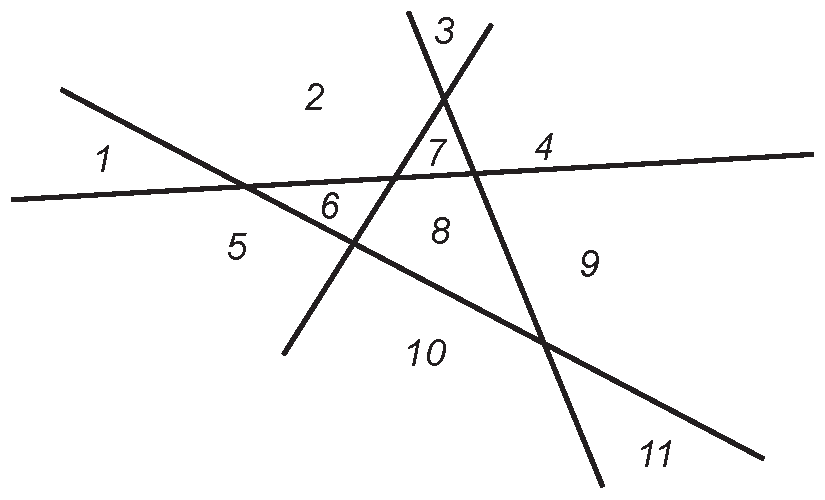
\includegraphics[scale=.6]{recurrence-figs/3012-fig9}\\
 \caption{\label{fig:geomregions}Lines and Regions} 
 \end{center}
 \end{figure}
how many regions a family of $1000$ lines would determine, given
these same restrictions on how the lines intersect.  More generally, let
$r_n$ denote the number of regions determined by $n$ lines.  Evidently,
$r_1=2$, $r_2=4$, $r_3=7$ and $r_4=11$.  Now it is easy to see that
we have the recurrence $r_{n+1} = r_n+n+1$.  To see this, choose any
one of the $n+1$ lines and call it $l$.  Line $l$ 
intersects each of the other lines and since no point in the plane
belongs to three or more lines, the points where $l$ intersects
the other lines are distinct.  Label them consecutively as
$x_1,x_2,\dots,x_n$.  Then these points divide line $l$ into
$n+1$ segments, two of which (first and last) are infinite.  Each of
these segments partitions one of the regions determined by the other
$n$ lines into two parts, meaning we have the $r_n$ regions determined
by the other $n$ lines and $n+1$ new regions that $l$ creates.

\section{Linear Recurrence Equations}\label{s:recurrence:linear}

What do all of the examples of the previous section have in common?
The end result that we were able to achieve is a \emph{linear
  recurrence}, which tells us how we can compute the $n^\text{th}$
term of a sequence given some number of previous values (and perhaps
also depending nonrecursively on $n$ as well, as in the last example).
More precisely a recurrence equation is said to be \textit{linear}
when it has the following form
\[
c_0a_{n+k}+ c_1a_{n+k-1} + c_2a_{n+k-2} + \dots+c_ka_{n} = g(n),
\] 
where $k\ge1$ is an integer, $c_0,c_1,\dots,c_k$ are constants with
$c_0,c_k\neq0$, and
$g:\ints\rightarrow\reals$ is a function. (What we have just defined
may more properly be called a linear recurrence equation with
\emph{constant coefficients}, since we require the $c_i$ to be
constants and prohibit them from depending on $n$. We will avoid this
additional descriptor, instead choosing to speak of linear recurrence
equations with \emph{nonconstant coefficients} in case we allow the
$c_i$ to be functions of $n$.) A linear equation is
\textit{homogeneous} if the function $g(n)$ on the right hand side
is the zero function.  For example, the Fibonacci sequence satisfies
the homogeneous linear recurrence equation
\[
a_{n+2} - a_{n+1} - a_n = 0.
\]
Note that in this example, $k=2$, $c_0=1$ and $c_k=-1$.

As a second example, the ternary sequence in
\hyperref[ex:recurrence:ternary-strings-no-20]{Example~\ref*{ex:recurrence:ternary-strings-no-20}}
  satifies the  homogeneous linear recurrence equation
\[
t_{n+2} - 3t_{n+1} + t_n = 0.
\]
Again, $k=2$ with $c_0=c_k=1$.

On the other hand, the sequence $r_n$ defined in
\autoref{s:recurrence:intro:lines} satisfies the nonhomogeneous
linear recurrence equation
\[
r_{n+1} - r_{n} = n+1.
\]
In this case, $k=1$, $c_0=1$ and $c_k=-1$.

Our immediate goal is to develop techniques for solving linear
recurrence equations of both homogeneous and nonhomogeneous types. We
will be able to fully resolve the question of solving homogeneous
linear recurrence equations and discuss a sort of ``guess-and-test''
method that can be used to tackle the more tricky nonhomogeneous type.

\section{Advancement Operators}\label{s:recurrence:adv-ops}

Much of our motivation for solving recurrence equations comes from an
analogous problem in continuous mathematics---differential
equations. You don't need to have studied these beasts before in order
to understand what we will do in the remainder of this chapter, but if
you have, the motivation for how we tackle the problems will be
clearer. As their name suggests, differential equations involve
derivatives, which we will denote using ``operator'' notation by $Df$
instead of the Leibniz notation $df/dx$. In our notation, the second
derivative is $D^2 f$, the third is $D^3 f$, and so on. Consider the
following example.

\begin{example}\label{ex:recurrence:diffeq}
  Solve the equation
  \[Df = 3f\] if $f(0) = 2$. Even if you've not studied differential
  equations, you should recognize that this question is really just
  asking us to find a function $f$ such that $f(0)=2$ and its
  derivative is three times itself. Let's ignore the \emph{initial
    condition} $f(0)=2$ for the moment and focus on the meat of the
  problem. What function, when you take its derivative, changes only
  by being multiplied by $3$?  You should quickly think of the
  function $e^{3x}$, since $D(e^{3x}) = 3e^{3x}$, which has exactly
  the property we desire. Of course, for any constant $c$, the
  function $ce^{3x}$ also satisfies this property, and this gives us
  the hook we need in order to satisfy our initial condition. We have
  $f(x) = ce^{3x}$ and want to find $c$ such that $f(0)=2$. Now $f(0)
  = c\cdot 1$, so $c=2$ does the trick and the solution to this very
  simple differential equation is $f(x) = 2e^{3x}$.
\end{example}

With differential equations, we apply the differential operator $D$ to
differentiable (usually infinitely differentiable) functions. For
recurrence equations, we consider the vector space $V$ whose elements
are functions from the set $\mathbb{Z}$ of integers to the set
$\mathbb{C}$ of complex numbers.  We then consider a function
$A:V\longrightarrow V$, called the 
\textit{advancement operator}, and defined by $A f(n) = f(n+1)$
(By various tricks and sleight of hand, we can extend a sequence 
$\{a_n\colon n\geq n_0\}$ to be a function whose domain is all of $\ints$, 
so this technique will apply to our problems). 
More generally, $A^p f(n)= f(n+p)$ when $p$ is
a positive integer.

\begin{example}
Let $f\in V$ be defined by $f(n)=7n-9$.  Then we apply the advancement
operator polynomial $3A^2-5A+4$ to $f$ with $n=0$ as follows:
\[
(3A^2-5A+4)f(0)=3f(2) - 5f(1) +4f(0)= 3(5)-5(-2)+4(-9)=-11.
\]
\end{example}

As an analogue of
\hyperref[ex:recurrence:diffeq]{Example~\ref*{ex:recurrence:diffeq}},
consider the following simple example involving the advancement
operator.

\begin{example}\label{ex:recurrence:adveq}
  Suppose that the sequence $\{s_n\colon n\geq 0\}$ satisfies $s_0 =
  3$ and $s_{n+1} = 2s_{n}$ for $n\geq 1$. Find an explicit formula
  for $s_n$.

  First, let's write the question in terms of the advancement
  operator. We can define a function $f(n) = s_n$ for $n\geq 0$, and
  then the information given becomes that $f(0)=3$ and
  \[Af(n) = 2f(n),\qquad n\geq 0.\]
  What function has the property that when we advance it, i.e.,
  evaluate it at $n+1$, it gives twice the value that it takes at $n$?
  The first function that comes into your mind should be $2^n$. Of
  course, just like with our differential equation, for any constant
  $c$, $c2^n$ also has this property. This suggests that if we take
  $f(n) = c2^n$, we're well on our way to solving our problem. Since
  we know that $f(0) = 3$, we have $f(0) = c2^0 = c$, so $c=
  3$. Therefore, $s_n = f(n) = 3\cdot 2^n$ for $n\geq 0$. This clearly
  satisfies our initial condition, and now we can check that it also
  satisfies our advancement operator equation:
  \[Af(n) = 3\cdot 2^{n+1} = 3\cdot 2\cdot 2^n = 2\cdot (3\cdot 2^n) =
  2\cdot f(n).\]
\end{example}

Before moving on to develop general methods for solving advancement
operator equations, let's say a word about why we keep talking in
terms of operators and mentioned that we can view any sequence as a
function with domain $\ints$. If you've studied any linear algebra, you
probably remember learning that the set of all
infinitely-differentiable functions on the real line form a vector
space and that differentiation is a linear operator on those
functions. Our analogy to differential equations holds up just fine
here, and functions from $\ints$ to $\mathbb{C}$ form a vector space and $A$ is a
linear operator on that space. We won't dwell on the technical aspects
of this, and no knowledge of linear algebra is required to understand
our development of techniques to solve recurrence equations. However,
if you're interested in more placing everything we do on rigorous
footing, we discuss this further in \autoref{s:recurrence:rigorous}.

\subsection{Constant Coefficient Equations}\label{s:recurrence:adv-ops:const-coeff}

It is easy to see that a linear recurrence equation can be
conveniently rewritten using a polynomial $p(A)$ of the 
advancement operator:
\begin{equation}\label{eqn:advance}
p(A)f=(c_0A^{k}+ c_1A^{k-1} + c_2A^{k-2} + \dots+c_k)f = g.
\end{equation} 
In equation~\ref{eqn:advance}, we intend that $k\ge1$ is an integer,
$g$ is a fixed vector (function) from $V$, and $c_0,c_1,\dots,
c_k$ are constants with $c_0,c_k\neq0$.  Note that since $c_0\neq0$,
we can divide both sides by $c_0$, i.e., we may in fact assume
that $c_0=1$ whenever convenient to do so.

\subsection{Roots and Factors}\label{s:recurrence:adv-ops:roots-factors}

The polynomial $p(A)$ can be analyzed like any other polynomial.
It has roots and factors, and although these may be difficult to
determine, we know they exist.  In fact, if the degree of $p(A)$ 
is $k$, we know that over the field of complex numbers, $p(A)$
has $k$ roots, counting multiplicities.  Note that since we assume
that $c_k\neq0$, all the roots of the polynomial $p$ are non-zero.

\subsection{What's Special About Zero?}\label{s:recurrence:adv-ops:zero}

Why have we limited our attention to recurrence equations of the form
$p(A)f = g$ where the constant term in $p$ is non-zero?  Let's
consider the alternative for a moment.  Suppose that the constant term
of $p$ is zero and that $0$ is a root of $p$ of multiplicity $m$.
Then $p(A) = A^mq(A)$ where the constant term of $q$ is non-zero.  And
the equation $p(A)f=g$ can then be written as $A^mq(A)f=g$.  To solve
this equation, we consider instead the simpler problem $q(A)f=g$.
Then $h$ is a solution of the original problem if and only if the
function $h'$ defined by $h'(n) = h(n+m)$ is a solution to the simpler
problem.  In other words, solutions to the original problem are just
translations of solutions to the smaller one, so we will for the most
part continue to focus on advancement operator equations where $p(A)$
has nonzero constant term, since being able to solve such problems is
all we need in order to solve the larger class of problems.

As a special case, consider the equation $A^m f =g$.  This requires
$f(n+m)=g(n)$, i.e., $f$ is just a translation of $g$.

\section{Solving advancement operator
  equations}\label{s:recurrence:solving}

In this section, we will explore some ways of solving advancement
operator equations. Some we will make up just for the sake of solving,
while others will be drawn from the examples we developed in
\autoref{s:recurrence:intro}. Again, readers familiar with
differential equations will notice many similarities between the
techniques used here and those used to solve linear differential
equations with constant coefficients, but we will not give any further
examples to make those parallels explicit.

\subsection{Homogeneous equations}\label{s:recurrence:solving:homogeneous}

Homogeneous equations, it will turn out, can be solved using very
explicit methodology that will work any time we can find the roots of
a polynomial. Let's start with another fairly straightforward example.

\begin{example}\label{ex:recurrence:deg2}
  Find all solutions to the advancement operator equation
  \begin{equation}(A^2+A-6)f = 0.\label{eqn:recurrence:deg2}\end{equation}

  Before focusing on finding \emph{all} solutions as we've been asked
  to do, let's just try to find \emph{some} solution. We start by noticing
  that here $p(A) = A^2+A-6 = (A+3)(A-2)$. With $p(A)$ factored like
  this, we realize that we've already solved part of this problem in
  \hyperref[ex:recurrence:adveq]{Example~\ref*{ex:recurrence:adveq}}!
  In that example, the polynomial of $A$ we encountered was (while not
  explicitly stated as such there) $A-2$. The solutions to $(A-2)f_1=0$
  are of the form $f_1(n) = c_12^n$. What happens if we try such a
  function here? We have
  \[(A+3)(A-2)f_1(n) = (A+3)0 = 0,\]
  so that $f_1$ is a solution to our given advancement operator
  equation. Of course, it can't be \emph{all} of them. However, it's
  not hard to see now that $(A+3)f_2 = 0$ has as a solution $f_2(n) =
  c_2(-3)^n$ by the same reasoning that we used in
  \hyperref[ex:recurrence:adveq]{Example~\ref*{ex:recurrence:adveq}}. Since
  $(A+3)(A-2) = (A-2)(A+3)$, we see right away that $f_2$ is also a
  solution of \autoref{eqn:recurrence:deg2}.

  Now we've got two infinite families of solutions to
  \autoref{eqn:recurrence:deg2}. Do they give us \emph{all} the
  solutions? It turns out that by combining them, they do in fact give
  all of the solutions. Consider what happens if we take $f(n) = c_1
  2^n + c_2 (-3)^n$ and apply $p(A)$ to it. We have
  \begin{align*}
    (A+3)(A-2)f(n) & = (A+3)(c_1 2^{n+1} + c_2 (-3)^{n+1} - 2(c_12^n +
    c_2(-3)^n))\\
    & = (A+3)(-5c_2(-3)^{n})\\
    & = -5c_2(-3)^{n+1}-15c_2(-3)^n\\
    & = 15c_2(-3)^n - 15c_2(-3)^n\\
    &=0.
  \end{align*}
  It's not all that hard to see that since $f$ gives a two-parameter family of
  solutions to \autoref{eqn:recurrence:deg2}, it gives us all the
  solutions, as we will show in detail in \autoref{s:recurrence:rigorous}.
\end{example}

What happened in this example is far from a fluke. If you have an
advancement operator equation of the form $p(A)f=0$ (the constant term
of $p$ nonzero) and $p$ has degree $k$, then the \emph{general
  solution} of $p(A)f=0$ will be a $k$-parameter family (in the
previous example, our parameters are the constants $c_1$ and $c_2$)
whose terms come from solutions to simpler equations arising from the
factors of $p$. We'll return to this thought in a little bit, but
first let's look at another example.

\begin{example}\label{ex:recurrence:ternary-strings-no-20-solved}
  Let's revisit the problem of enumerating ternary strings of length
  $n$ that do have $(2,0)$ occurring as a substring in two consecutive
  positions that we encountered in
  \hyperref[ex:recurrence:ternary-strings-no-20]{Example~\ref*{ex:recurrence:ternary-strings-no-20}}. There
  we saw that this number satisfies the recurrence equation
  \[t_{n+2} = 3t_{n+1} - t_n,\qquad n\geq 1\]
  and $t_1 = 3$ and $t_2=8$. Before endeavoring to solve this, let's
  rewrite our recurrence equation as an advancement operator
  equation. This gives us
  \begin{equation}
    \label{eqn:recurrence:ternary}
    p(A)t=(A^2-3A+1)t=0.
  \end{equation}
  The roots of $p(A)$ are $(3\pm\sqrt{5})/2$. Following the approach
  of the previous example, our general solution is
  \[t(n) = c_1\left(\frac{3+\sqrt{5}}{2}\right)^n +
  c_2\left(\frac{3-\sqrt{5}}{2}\right)^n.\]
  This probably looks suspicious; we're \emph{counting strings} here,
  so $t(n)$ needs to be a nonnegative integer, but the form we've
  given includes not just fractions but also square roots! However,
  if you look carefully, you'll see that using the binomial theorem to
  expand the terms in our expression for $t(n)$ would get rid of all
  the square roots, so everything is good. (A faster way to convince
  yourself that this really satisfies \autoref{eqn:recurrence:ternary}
  is to mimic the verification we used in the previous example.)
  Because we have initial values for $t(n)$, we are able to solve for
  $c_1$ and $c_2$ here. Evaluating at $n=0$ and $n=1$ we get
  \begin{align*}
    3 &= c_1 + c_2\\
    8 & = c_1\frac{3+\sqrt{5}}{2} + c_2 \frac{3-\sqrt{5}}{2}.
  \end{align*}
  A little bit of computation gives
  \[c_1 = \frac{7\sqrt{5}}{10} + \frac{3}{2} \quad\text{and}\quad c_2 =
  -\frac{7\sqrt{5}}{10} +\frac{3}{2}\]
  so that
  \[t(n) = \left(\frac{7\sqrt{5}}{10} + \frac{3}{2}\right)
  \left(\frac{3+\sqrt{5}}{2}\right)^n+ \left(-\frac{7\sqrt{5}}{10}
    +\frac{3}{2}\right) \left(\frac{3-\sqrt{5}}{2}\right)^n.\]
\end{example}

\begin{example}
  Find the general solution to the advancement operator equation
  \[(A+1)(A-6)(A+4)f = 0.\]
  
  By now, you shouldn't be surprised that we immediately make use of
  the roots of $p(A)$ and have that the solution is
  \[f(n) = c_1(-1)^n + c_2 6^n + c_3 (-4)^n.\]
\end{example}

By now, you should be able to see most of the pattern for solving
homogeneous advancement operator equations. However, the examples
we've considered thus far have all had one thing in common: the roots
of $p(A)$ were all distinct. Solving advancement operator equations in
which this is not the case is not much harder than what we've done so
far, but we do need to treat it as a distinct case.

\begin{example}\label{ex:recurrence:deg2-repeated}
  Find the general solution of the advancement operator equation
  \[(A-2)^2 f=0.\]
  
  Here we have the repeated root problem that we mentioned a moment
  ago. We see immediately that $f_1(n) = c_12^n$ is a solution to this
  equation, but that can't be all, as we mentioned earlier that we
  must have a $2$-parameter family of solutions to such an
  equation. You might be tempted to try $f_2(n) = c_2 2^n$ and $f(n) =
  f_1(n) + f_2(n)$, but then this is just $(c_1+c_2)2^n$, which is
  really just a single parameter, $c=c_1+c_2$.

  What can we do to resolve this conundrum? What if we tried $f_2(n) =
  c_2 n2^n$? Again, if you're familiar with differential equations,
  this would be the analogous thing to try, so let's give it a
  shot. Let's apply $(A-2)^2$ to this $f_2$. We have
  \begin{align*}
    (A-2)^2 f_2(n) &= (A-2)(c_2(n+1)2^{n+1} - 2c_2 n2^n)\\
    & = (A-2)(c_2 2^{n+1})\\
    & = c_22^{n+2} - 2c_2 2^{n+1}\\
    & = 0.
  \end{align*}
  Since $f_2$ satisfies our advancement operator equation, we have
  that the general solution is
  \[f(n) = c_1 2^n + c_2 n2^n.\]
\end{example}

\begin{example}\label{ex:recurrence:deg4-repeated}
  Consider the recurrence equation
  \[f_{n+4} = -2f_{n+3} + 12f_{n+2} + -14 f_{n+1} + 5f_n\]
  with initial conditions $f_0 = 1$, $f_1= 2$, $f_2 = 4$, and $f_3 =
  4$. Find an explicit formula for $f_n$.

  We again start by writing the given recurrence equation as an
  advancement operator equation for a function $f(n)$:
  \begin{equation}
    \label{eqn:recurrence:deg4-repeated}
    (A^4 +2A^3 -12A^2+14A-5)f = 0.
  \end{equation}
  Factoring $p(A) = A^4 +2A^3 -12A^2+14A-5$ gives $p(A) =
  (A+5)(A-1)^3$. Right away, we see that $f_1(n) = c_1 (-5)^n$ is a
  solution. The previous example should have you convinced that
  $f_2(n) = c_2\cdot 1^n = c_2$ and $f_3(n) = c_3 n \cdot 1^n = c_3 n$
  are also solutions, and it's not likely to surprise you when we
  suggest trying $f_4(n) = c_4 n^2$ as another solution. To verify
  that it works, we see
  \begin{align*}
    (A+5)(A-1)^3 f_4(n) &= (A+5)(A-1)^2(c_4(n+1)^2 - c_4 n^2)\\
    & = (A+5)(A-1)^2 (2c_4 n + c_4)\\
    & = (A+5)(A-1)(2c_4(n+1) + c_4 - 2c_4 n -c_4)\\
    & = (A+5)(A-1)(2c_4)\\
    & = (A+5)(2c_4-2c_4)\\
    &= 0.
  \end{align*}
  Thus, the general solution is
  \[f(n) = c_1 (-5)^n + c_2 + c_3 n + c_4n^2.\]
  Since we have initial conditions, we see that
  \begin{align*}
    1= f(0) & = c_1+c_2\\
    2 = f(1) & = -5c_1 + c_2 + c_3 + c_4\\
    4 = f(2) & = 25c_1 + c_2 + 2c_3 + 4c_4\\
    4 = f(3) & = -125c_1 + c_2 +3c_3 +9c_4
  \end{align*}
  is a system of equations whose solution gives the values for the
  $c_i$. Solving this system gives that the desired solution is
  \[f(n) = \frac{1}{72} (-5)^n +\frac{71}{72} + \frac{5}{6} n +\frac{1}{4} n^2.\]
\end{example}

\subsection{Nonhomogeneous equations}\label{s:recurrence:solving:nonhomogeneous}

As we mentioned earlier, nonhomogeneous equations are a bit trickier
than solving homogeneous equations, and sometimes our first attempt at
a solution will not be successful but will suggest a better function
to try. Before we're done, we'll revisit the problem of lines in the
plane that we've considered a couple of times, but let's start with a
more illustrative example.

\begin{example}
  Consider the advancement operator equation
  \[(A+2)(A-6)f=3^n.\]
  Let's try to find the general solution to this, since once we have
  that, we could find the specific solution corresponding to any given
  set of initial conditions.

  When dealing with nonhomogeneous equations, we proceed in two
  steps. The reason for this will be made clear in
  \hyperref[lem:particular]{Lemma~\ref*{lem:particular}}, but let's
  focus on the method for the moment. Our first step is to find the
  general solution of the homogeneous equation corresponding to the
  given nonhomogeneous equation. In this case, the homogeneous
  equation we want to solve is
  \[(A+2)(A-6)f=0,\]
  for which by now you should be quite comfortable in rattling off a
  general solution of 
  \[f_1(n) = c_1 (-2)^n + c_2 6^n.\]
  Now for the process of actually dealing with the nonhomogeneity of
  the advancement operator equation. It actually suffices to find
  \emph{any} solution of the nonhomogeneous equation, which we will
  call a \emph{particular} solution. Once we have a particular
  solution $f_0$ to the equation, the general solution is simply
  $f=f_0 + f_1$, where $f_1$ is the general solution to the
  homogeneous equation.

  Finding a particular solution $f_0$ is a bit trickier than finding
  the general solution of the homogeneous equation. It's something for
  which you can develop an intuition by solving lots of problems, but
  even with a good intuition for what to try, you'll still likely find
  yourself having to try more than one thing on occasion in order to
  get a particular solution. What's the best starting point for this
  intuition? It turns out that the best thing to try is usually (and
  not terribly surprisingly) something that looks a lot like the right
  hand side of the equation, but we will want to include one or more
  new constants
  to help us actually get a solution. Thus, here we try $f_0(n) = d 3^n$. We
  have
  \begin{align*}
    (A+2)(A-6)f_0(n) &= (A+2)(d3^{n+1}-6d3^n)\\
    & = (A+2)(-d3^{n+1})\\
    & = -d3^{n+2} -2d3^{n+1}\\
    & = -5d 3^{n+1}
  \end{align*}
  We want $f_0$ to be a solution to the nonhomogeneous equation,
  meaning that $(A+2)(A-6)f_0 = 3^n$. This implies that we need to
  take $d=-1/15$. Now, as we mentioned earlier, the general solution
  is
  \[f(n) = f_0(n) + f_1(n) = -\frac{1}{15}3^n + c_1 (-2)^n + c_2
  6^n.\]
  We leave it to you to verify that this does satisfy the given equation.
\end{example}

% Do we want another "basic" example before we jump into the problems
% that might arise?

You hopefully noticed that in the previous example, we said that the
first guess to try for a particular solution looks a lot like right
hand side of the equation, rather than exactly like. Our next example
will show why we can't always take something that matches exactly.

\begin{example}
  Find the solution to the advancement operator equation
  \[(A+2)(A-6)f=6^n\]
  if $f(0) = 1$ and $f(1) = 5$.

  The corresponding homogeneous equation here is the same as in the
  previous example, so its general solution is again $f_1(n) =
  c_1(-2)^n + c_2 6^n$. Thus, the real work here is finding a
  particular solution $f_0$ to the given advancement operator
  equation. Let's just try what our work on the previous example would
  suggest here, namely $f_0(n) = d6^n$. Applying the advancement
  operator polynomial $(A+2)(A-6)$ to $f_0$ then gives, uh, well,
  zero, since $(A-6)(d6^n) = d6^{n+1}-6d6^n =0$. Huh, that didn't work
  out so well. However, we can take a cue from how we tackled
  homogeneous advancement operator equations with repeated roots and
  introduce a factor of $n$. Let's try $f_0(n) = dn6^n$. Now we have
  \begin{align*}
    (A+2)(A-6)(dn6^n) &= (A+2)(d(n+1)6^{n+1}-6dn6^n)\\
    &= (A+2)d6^{n+1}\\
    &= d6^{n+2} + 2d 6^{n+1}\\
    &= 6^n(36d+12d) = 48d6^n.
  \end{align*}
  We want this to be equal to $6^n$, so we have $d = 1/48$. Therefore,
  the general solution is
  \[f(n) = \frac{1}{48}n6^n + c_1 (-2)^n + c_2 6^n.\]
  All that remains is to use our initial conditions to find the
  constants $c_1$ and $c_2$. We have that they satisfy the following
  pair of equations:
  \begin{align*}
    1 & = c_1 + c_2\\
    5 & = \frac{1}{8} -2c_1+6c_2
  \end{align*}
  Solving these, we arrive at the desired solution, which is
  \[f(n) = \frac{1}{48}n6^n + \frac{9}{64} (-2)^n + \frac{55}{64} 6^n.\]
\end{example}

What's the lesson we should take away from this example? When making a
guess at a particular solution of a nonhomogeneous advancement
operator equation, it does us no good to use any terms that are also
solutions of the corresponding homogeneous equation, as they will be
annihilated by the advancement operator polynomial. Let's see how this
comes into play when finally resolving one of our longstanding examples.

\begin{example}\label{ex:recurrence:lines-solved}
  We're now ready to answer the question of how many regions are
  determined by $n$ lines in the plane in general position as we
  discussed in \autoref{s:recurrence:intro:lines}. We have the
  recurrence equation
  \[r_{n+1} = r_n + n+1,\]
  which yields the nonhomogeneous advancement operator equation
  $(A-1)r = n+1$. As usual, we need to start with the general
  solution to the corresponding homogeneous equation. This solution is
  $f_1(n) = c_1$. Now our temptation is to try $f_0(n)=d_1n+d_2$ as a
  particular solution. However since the constant term there is a
  solution to the homogeneous equation, we need a bit more. Let's try
  increasing the powers of $n$ by $1$, giving $f_0(n) = d_1n^2 +
  d_2n$. Now we have
  \begin{align*}
    (A-1)(d_1n^2+d_2n) & = d_1(n+1)^2+d_2(n+1) - d_1n^2 -d_2n\\
    & = 2d_1n+d_1+d_2.
  \end{align*}
  This tells us that we need $d_1=1/2$ and $d_2=1/2$, giving $f_0(n) =
  n^2/2 + n/2$. The general solution is then
  \[f(n) = c_1 + \frac{n^2+n}{2}.\]
  What is our initial condition here? Well, one line divides the plane
  into two regions, so $f(1) = 2$. On the other hand, $f(1) = c_1 +
  1$, so $c_1=1$ and thus
  \[f(n) = 1 + \frac{n^2+n}{2} = \binom{n+1}{2} + 1\]
  is the number of regions into which the plane is divided by $n$
  lines in general position.
\end{example}

We conclude this section with one more example showing how to deal
with a nonhomogeneous advancement operator equation in which the right
hand side is of ``mixed type''.

\begin{example}
  Give the general solution of the advancement operator equation
  \[(A-2)^2 f = 3^n + 2n.\]
  
  Finding the solution to the corresponding homogeneous equation is
  getting pretty easy at this point, so just note that
  \[f_1(n) = c_1 2^n + c_2 n2^n.\]
  What should we try as a particular solution? Fortunately, we have no
  interference from $p(A)=(A-2)^2$ here. Our first instinct is
  probably to try $f_0(n) = d_1 3^n + d_2 n$. However, this won't
  actually work. (Try it. You wind up with a leftover constant term
  that you can't just make zero.) The key here is that if we use a
  term with a nonzero power of $n$ in it, we need to include the lower
  order powers as well (so long as they're not superfluous because of
  $p(A)$). Thus, we try
  \[f_0(n) = d_1 3^n + d_2 n + d_3.\]
  This gives
  \begin{align*}
    (A-2)^2(d_1 3^n + d_2 n + d_3) & = (A-2)(d_13^{n+1} + d_2(n+1)+d_3
    - 2d_1 3^n - 2d_2 n -2d_3)\\
    & = (A-2)(d_13^n - d_2n + d_2 -d_3)\\
    & = d_1 3^{n+1} - d_2(n+1) + d_2 - d_3 - 2 d_1 3^n + 2d_2 n -2d_2
    + 2d_3\\
    & = d_1 3^n + d_2 n -2d_2 + d_3.
  \end{align*}
  We want this to be $3^n+2n$, so matching coefficients gives $d_1 =
  1$, $d_2 =2$, and $d_3=4$. Thus, the general solution is
  \[f(n) = 3^n+2n+4 + c_1 2^n + c_2 n 2^n.\]
\end{example}

\section{Formalizing our approach to recurrence equations}\label{s:recurrence:rigorous}

So far, our approach to solving recurrence equations has been based on
intuition, and we've not given a lot of explanation for why the
solutions we've given have been the general solution. In this section,
we endeavor to remedy this. Some familiarity with the language of
linear algebra will be useful for the remainder of this section, but
it is not essential.

Our techniques for solving recurrence equations have their roots in a
fundamentally important concept in mathematics, the notion of a vector
space.  Recall that a vector space\footnote{ To be more complete, we
  should say that we are talking about a vector space over the field
  of real numbers, but in our course, these are the only kind of
  vector spaces we will consider.  For this reason, we just use the
  short phrase ``vector space''.} consists of a set $V$ of elements
called \textit{vectors}; in addition, there is a binary operation
called \textit{addition} with the sum of vectors $x$ and $y$ denoted
by $x+y$; furthermore, there is an operation called \textit{scalar
  multiplication} or \textit{scalar product} which combines a scalar
(real number) $\alpha$ and a vector $x$ to form a product denoted
$\alpha x$.  These operations satisfy the following properties.

\begin{enumerate}
\item  $x+y=y+x$ for every $x,y,\in V$.
\item  $x+(y+z) = (x+y)+z$, for every $x,y,z\in V$.
\item There is a vector called \textit{zero} and denoted $0$ so that
  $x+0=x$ for every $x\in V$. \textit{Note:} We are again overloading
  an operator and using the symbol $0$ for something other than a
  number.
\item For every element $x\in V$, there is an element $y\in V$, called
  the \textit{additive inverse} of $x$ and denoted $-x$ so that
  $x+(-x)=0$.  This property enables us to define
  \textit{subtraction}, i.e., $x-y= x+(-y)$.
\item $1x=x$ for every $x\in X$.
\item $\alpha(\beta x) = (\alpha\beta)x$, for every
  $\alpha,\beta\in\reals$ and every $x\in V$.
\item $\alpha(x+y)=\alpha x + \alpha y$ for every $\alpha\in\reals$
  and every $x,y\in V$.
\item $(\alpha +\beta) x = \alpha x + \beta x$, for every
  $\alpha,\beta\in\reals$ and every $x\in V$.
\end{enumerate}

When $V$ is a vector space, a function $\phi:V\rightarrow V$ is called
an \textit{linear operator}, or just \textit{operator} for short, when
$\phi(x+y)=\phi(x)+\phi(y)$ and $\phi(\alpha x)=\alpha\phi(x)$.  When
$\phi:V\rightarrow V$ is an operator, it is customary to write $\phi
x$ rather than $\phi(x)$, saving a set of parentheses.  The set of all
operators over a vector space $V$ is itself a vector space with
addition defined by $(\phi+\rho)x = \phi x +\rho x$ and scalar
multiplication by $(\alpha\phi)x=\alpha(\phi x)$.

In this chapter, we focus on the real vector space $V$ consisting of
all functions of the form $f:\ints\rightarrow\reals$.  Addition is
defined by $(f+g)(n)= f(n)+g(n)$ and scalar multiplication is defined
by $(\alpha f)(n)=\alpha(f(n))$.

\subsection{The Principal Theorem}\label{s:recurrence:rigorous:principal}
Here is the basic theorem about solving recurrence equations (stated
in terms of advancement operator equations)---and while we won't prove
the full result, we will provide enough of an outline where it
shouldn't be too difficult to fill in the missing details.

\begin{theorem}\label{thm:advance}
Let $k$ be a positive integer $k$, and let $c_0,c_1,\dots,c_k$ be
constants with $c_0,c_k\neq 0$.  Then the set $W$ of all solutions to the
homogeneous linear equation
\begin{equation}
(c_0A^{k}+ c_1A^{k-1} + c_2A^{k-2} + \dots+c_k)f = 0
\end{equation} 
is a $k$-dimensional subspace of $V$.
\end{theorem}

The conclusion that the set $W$ of all solutions is a subspace
of $V$ is immediate, since
\[
p(A)(f+g)=p(A)f+p(A)g\quad\text{ and }\quad p(a)(\alpha f)=\alpha p(A)(f).
\]  
What takes a bit of work is to show that $W$ is a 
$k$-dimensional subspace.  But once this is done,
then to solve the advancement operator 
equation given in the form of \autoref{thm:advance}, it 
suffices to find a \textit{basis} for the vector space $W$.  
Every solution is just a linear combination of basis vectors.
In the next several sections, we outline
how this goal can be achieved.

\subsection{The Starting Case}\label{s:recurrence:rigorous:start}

The development proceeds by induction (surprise!) with
the case $k=1$ being the base case.  In this case, we study
a simple equation of the form $(c_0A+c_1)f=0$.  Dividing by
$c_0$ and rewriting using subtraction rather than addition, it
is clear that we are just talking about an equation of the form
$(A-r)f=0$ where $r\neq0$.

\begin{lemma}\label{lem:base}
Let $r\neq0$,and let $f$ be a solution to the operator equation $(A-r)f=0$,
Then let $c=f(0)$.  Then $f(n)=cr^n$ for every
$n\in \ints$.
\end{lemma}

\begin{proof}  We first show that $f(n)=cr^n$ for every
$n\ge0$, by induction on $n$.  The base case is trivial since
$c=f(0) = cr^0$.  Now suppose that $f(k)=cr^k$ for some non-negative
integer $k$.  Then $(A-r)f=0$ implies that $f(k+1)-rf(k)=0$, i.e.,
\[
f(k+1)=rf(k)= rcr^k=cr^{k+1}.
\]
A very similar argument shows that $f(-n) = cr^{-n}$ for
every $n\le0$.
\end{proof}

\begin{lemma}\label{lem:particular}
Consider a nonhomogeneous operator equation of the form
\begin{equation}\label{eqn:nonhomogeneous}
p(A)f= (c_0A^{k}+ c_1A^{k-1} + c_2A^{k-2} + \dots+c_k)f = g,
\end{equation}
with $c_0,c_k\neq0$,
and let $W$ be the subspace of $V$ consisting of all solutions
to the corresponding homogeneous equation
\begin{equation}\label{eqn:homogeneous}
p(A)f=(c_0A^{k}+ c_1A^{k-1} + c_2A^{k-2} + \dots+c_k)f = 0.
\end{equation}

If $f_0$ is a solution to \autoref{eqn:nonhomogeneous}, then every
solution $f$ to \autoref{eqn:nonhomogeneous} has the form
$f=f_0+f_1$ where $f_1\in W$.
\end{lemma}
\begin{proof}
Let $f$ be a solution of \autoref{eqn:nonhomogeneous}, and let
$f_1=f-f_0$.
Then
\[
p(A)f_1 = p(A)(f-f_0)=p(A)f-p(A)f_0=g-g=0.
\]
This implies that $f_1\in W$ and that $f=f_0+f_1$ so that all
solutions to \autoref{eqn:nonhomogeneous} do in fact have the desired
form.
\end{proof}

Using the preceding two results, we can now provide an outline of the
inductive step in the proof of \autoref{thm:advance}, at least in the
case where the polyomial in the advancement operator has distinct
roots.

\begin{theorem}
Consider the following advancement operator equation
\begin{equation}\label{eqn:distinct}
p(A)f=(A-r_1)(A-r_2)\dots(A-r_k)f=0.
\end{equation}
with $r_1,r_2,\dots,r_k$ distinct non-zero constants.
Then every solution
to \autoref{eqn:distinct} has the form
\[
f(n)=c_1r_1^n+c_2 r_2^n+c_3r_3^n+\dots+c_kr_k^n.
\]
\end{theorem}
\begin{proof}
  The case $k=1$ is \hyperref[lem:base]{Lemma~\ref*{lem:base}}.  Now
  suppose we have established the theorem for some positive integer
  $m$ and consider the case $k=m+1$. Rewrite \autoref{eqn:distinct} as
  \[
  (A-r_1)(A-r_2)\dots(A-r_m)[(A-r_{m+1})f]=0.
  \]
  By the inductive hypothesis, it follows that if $f$ is a solution to
  \autoref{eqn:distinct}, then $f$ is also a solution to the
  nonhomogeneous equation
  \begin{equation}\label{eqn:distinct2}
    (A-r_{m+1})f=d_1r_1^n+d_2r_2^n+\dots+d_mr_m^n.
  \end{equation}
  To find a particular solution $f_0$ to \autoref{eqn:distinct2},
  we look for a solution having the form
  \begin{equation}\label{eqn:distinct3}
    f_0(n)= c_1 r_1^n+c_2 r_2^n+\dots+c_m r_m^n.
  \end{equation}
  On the other hand, a simple calculation shows that for each
  $i=1,2,\dots,m$, we have
  \[
  (A-r_{m+1})c_i r_i^n=c_i r_i^{n+1}-r_{m+1}c_i r_i^n=c_i (r_i-r_{m+1})r_i^n,
  \]
  so it suffices to choose $c_i$ so that $c_i(r_i-r_{m+1})=d_i$, for each
  $i=1,2,\dots,m$. This can be done since $r_{m+1}$ is distinct from
  $r_i$ for $i=1,2,\dots m$.

  So now we have a particular solution $f_0(n)=\sum_{i=1}^{m} c_i
  r_i^n$.  Next we consider the corresponding homogeneous equation
  $(A-r_{m+1})f=0$.  The general solution to this equation has the
  form $f_1(n)=c_{m+1}r_{m+1}^n$.  It follows that every solution to
  the original equation has the form
  \[
  f(n)=f_0(n)+f_1(n) = c_1r_1^n+c_2r_2^n+\dots+c_m r_m^n+cr_{m+1}^n,
  \]
  which is exactly what we want!
\end{proof}

\subsection{Repeated Roots}\label{s:recurrence:rigorous:repeated}

It is straightforward to modify the proof given in the preceding
section to obtain the following result.  We leave the details as an
exercise.
\begin{lemma}\label{lem:rr}
  Let $k\ge1$ and consider the equation
  \begin{equation}\label{eqn:rr}
    (A-r)^kf=0.
  \end{equation}
  Then the general solution to \autoref{eqn:rr} has the following form
  \begin{equation}\label{eqn:solutionrr}
    f(n)=c_1r^n+c_2nr^n+c_3n^2r^n+c_4n^3r^n+\dots+c_kn^{k-1}r^n.
  \end{equation}
\end{lemma}

\subsection{The General Case}\label{s:recurrence:rigorous:general}

Combining the results in the preceding sections, we can quickly write
the general solution of any homogeneous equation of the form $p(A)f=0$
\textit{provided} we can factor the polynomial $p(A)$.  Note that in
general, this solution takes us into the field of \textit{complex
  numbers}, since the roots of a polynomial with real coefficients are
sometimes complex numbers---with non-zero imaginary parts.

We close this section with one more example which illustrates how
quickly we can read off the general solution of a homogeneous
advancement operator equation $p(A)f=0$, provided that $p(A)$ is
factored.

\begin{example}
Consider the advancement operator equation
\[
(A-1)^5(A+1)^3(A-3)^2(A+8)(A-9)^4f=0.
\]
Then every solution has the following form
\begin{align*}
f(n)=&c_1+c_2n+c_3n^2+c_4n^3+c_5n^4\\
     &+c_6(-1)^n+c_7n(-1)^n+c_8n^2(-1)^n\\
     &+c_93^n+c_{10}n3^n\\
     &+c_{11}(-8)^n\\
     &+c_{12}9^n +c_{13}n 9^n+c_{14}n^2 9^n +c_{15}n^39^n.
\end{align*}

\end{example}

\section{Using generating functions to solve recurrences}\label{s:recurrence:genfunction}

The approach we have seen thus far in this chapter is not the only way
to solve recurrence equations. Additionally, it really only applies to
linear recurrence equations with constant coefficients. In the
remainder of the chapter, we will look at some examples of how
generating functions can be used as another tool for solving
recurrence equations. In this section, our focus will be on linear
recurrence equations. In \autoref{s:recurrence:rubots}, we will see
how generating functions can solve a nonlinear recurrence.

Our first example is the homogeneous recurrence that corresponds to
the advancement operator equation in
\hyperref[ex:recurrence:deg2]{Example~\ref*{ex:recurrence:deg2}}.

\begin{example}\label{ex:recurrence:gf-homog}
  Consider the recurrence equation $r_{n}+r_{n-1}-6r_{n-2} = 0$ for the
  sequence $\{r_n\colon n\geq 0\}$ with $r_0=1$ and $r_1=3$. This
  sequence has generating function
  \[f(x) = \sum_{n=0}^\infty r_n x^n = r_0+r_1
  x+r_2x^2+r_3x^3+\cdots.\]
  Now consider for a moment what the function $xf(x)$ looks like. It
  has $r_{n-1}$ as the coefficient on $x_n$. Similarly, in the
  function $-6x^2 f(x)$, the coefficient on $x^n$ is $-6r_{n-2}$. 

  What is our point in all of this? Well, if we add them all up,
  notice what happens. The coefficient on $x_n$ becomes
  $r_n+r_{n-1}-6r_{n-2}$, which is $0$ because of the recurrence
  equation! Now let's see how this all lines up:
  \begin{align*}
    f(x) &= r_0 + r_1 x + r_2x^2 + r_3 x^3 + \cdots + r_nx^n + \cdots\\
    xf(x) &= 0 + r_0 x + r_1x^2 + r_2 x^3 + \cdots r_{n-1}x^n + \cdots\\
    -6x^2f(x) & = 0 + 0 -6r_0x^2 - 6r_1 x^3 + \cdots - 6r_{n-2}x^n + \cdots
  \end{align*}
  When we add the left-hand side, we get $f(x)(1+x-6x^2)$. On the
  right-hand side, the coefficient on $x^n$ for $n\geq 2$ is $0$
  because of the recurrence equation. However, we are left with $r_0 +
  (r_0+r_1)x = 1 + 4x$, using the initial conditions. Thus, we have
  the equation
  \[f(x)(1+x-6x^2)= 1+4x,\]
  or $f(x) = (1+4x)/(1+x-6x^2)$. This is a generating function that we
  can attack using partial fractions, and we find that
  \[f(x) = \frac{6}{5}\frac{1}{1-2x}-\frac{1}{5}\frac{1}{1+3 x} =
  \frac{6}{5}\sum_{n=0}^\infty 2^n x^n -\frac{1}{5} \sum_{n=0}^\infty
  (-3)^n x^n.\]
  From here, we read off $r_n$ as the coefficient on $x^n$ and
  have $r_n = (6/5) 2^n -(1/5)(-3)^n$.
\end{example}

Although there's a bit more work involved, this method can be used to
solve nonhomogeneous recurrence equations as well, as the next example
illustrates.

\begin{example}\label{ex:recurrence:gf-nonhomog}
  The recurrence equation $r_n - r_{n-1}-2r_{n-2} = 2^n$ is
  nonhomogeneous. Let $r_0=2$ and $r_1=1$. This time, to solve the
  recurrence, we start by multiplying both sides by $x^n$. This gives
  the equation
  \[r_nx^n - r_{n-1}x^n-2r_{n-2}x^n = 2^nx^n.\]
  If we sum this over all values of $n\geq 2$, we have
  \[\sum_{n=2}^\infty r_nx^n - \sum_{n=2}^\infty r_{n-1}x^n-2
  \sum_{n=2}^\infty r_{n-2}x^n = \sum_{n=2}^\infty 2^nx^n.\]
  The right-hand side you should readily recognize as being almost equal to
  $1/(1-2x)$. We are missing the $1$ and $2x$ terms, however, so
  must subtract them from the rational function form of the series. On the left-hand side, however, we need to do a bit more
  work.

  The first sum is just missing the first two terms of the series, so
  we can replace it by $R(x) - (2+x)$, where $R(x)=\sum_{n=0}^\infty
  r_n x^n$. The second sum is almost $xR(x)$, except it's missing the
  first term. Thus, it's equal to $xR(x) - 2x$. The sum in the final
  term is simply $x^2 R(x)$. Thus, the equation can be rewritten as
  \[R(x) - (2+x) -(xR(x)-2x)-2x^2R(x) = \frac{1}{1-2x} - 1- 2x.\]
  A little bit of algebra then gets us to the generating function
  \[R(x) = \frac{6x^2-5x+2}{2(1-2x)(1-x-2x^2)}.\]
  This generating function can be expanded using partial fractions, so
  we have
  \begin{align*}
    R(x) &= -\frac{1}{9(1-2x)} + \frac{2}{3(1-2x)^2} +
    \frac{13}{9(1+x)}\\ 
    &= -\frac{1}{9} \sum_{n=0}^\infty 2^nx^n +
    \frac{2}{3}\sum_{n=0}^\infty n2^{n-1} x^{n-1} +
    \frac{13}{9}\sum_{n=0}^\infty (-1)^n.\end{align*}
  From this generating function, we can now read off that
  \[r_n = -\frac{1}{9}2^n + \frac{2(n+1)}{3}2^{n} + \frac{13}{9}(-1)^n =
  \frac{5}{9} 2^n + \frac{2}{3}n2^n + \frac{13}{9}(-1)^n.\]
\end{example}

The recurrence equations of the two examples in this section can both
be solved using the techniques we studied earlier in the chapter. One
potential benefit to the generating function approach for
nonhomogeneous equations is that it does not require determining an
appropriate form for the particular solution. However, the method of
generating functions often requires that the resulting generating
function be expanded using partial fractions. Both approaches have
positives and negatives, so unless instructed to use a specific
method, you should choose whichever seems most appropriate for a given
situation. In the next section, we will see a recurrence equation that
is most easily solved using generating functions because it is
nonlinear.

\section{Solving a nonlinear recurrence}\label{s:recurrence:rubots}

In this section, we will use generating functions to enumerate the a
certain type of trees. In doing this, we will see how generating
functions can be used in solving a \emph{nonlinear} recurrence
equation. We will also make a connection to a counting sequence we
encountered back in \autoref{ch:strings}. To do all of this, we must
introduce a bit of terminology. A tree is \emph{rooted} if we have
designated a special vertex called its \emph{root}. We will always
draw our trees with the root at the top and all other vertices below
it. An \emph{unlabeled} tree is one in which we do not make
distinctions based upon names given to the vertices. For our purposes,
a \emph{binary} tree is one in which each vertex has $0$ or $2$
children, and an \emph{ordered} tree is one in which the children of a
vertex have some ordering (first, second, third, etc.). Since we will
be focusing on rooted, unlabeled, binary, ordered trees (RUBOTs for
short), we will call the two children of vertices that have children
the \emph{left} and \emph{right} children.

In \autoref{fig:rubots}, we show the rooted, unlabeled, binary, ordered
trees with $n$ leaves for $n\leq 4$.

\begin{figure}[h]
  \centering
  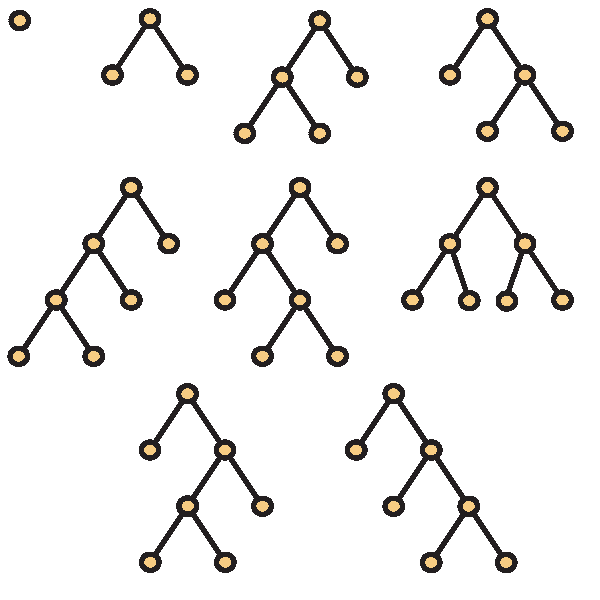
\includegraphics{recurrence-figs/RUBOTs}
  \caption{The RUBOTs with $n$ leaves for $n\leq 4$}
  \label{fig:rubots}
\end{figure}

Let $C(x) = \sum_{n=0}^\infty c_n x^n$ be the generating function for
the sequence $\{c_n\colon n\geq 0\}$ where $c_n$ is the number of
RUBOTs with $n$ leaves. (We take $c_0=0$ for convenience.) Then we can
see from \autoref{fig:rubots} that $C(x) = x + x^2 + 2x^3 + 5x^4 +
\cdots$. But what are the remaining coefficients? Let's see how we can
break a RUBOT with $n$ leaves down into a combination of two smaller
RUBOTs to see if we can express $c_n$ in terms of some $c_k$ for $k<
n$. When we look at a RUBOT with $n\geq 2$ leaves, we notice that the
root vertex must have two children. Those children can be viewed as
root nodes of smaller RUBOTs, say the left child roots a RUBOT with
$k$ leaves, meaning that the right child roots a RUBOT with $n-k$
leaves. Since there are $c_k$ possible sub-RUBOTs for the left child
and $c_{n-k}$ sub-RUBOTs for the right child, there are a total of
$c_kc_{n-k}$ RUBOTs in which the root's left child has $k$ leaves on
its sub-RUBOT. We can do this for any $k=1,2,\dots,n-1$, giving us
that
\[c_n = \sum_{k=1}^{n-1} c_kc_{n-k}.\]
(This is valid since $n\geq 2$.)
Since $c_0=0$, we can actually write this as
\[c_n = \sum_{k=0}^{n} c_kc_{n-k}.\]

Let's look at the square of the generating function $C(x)$. By
\hyperref[prop:genfunction-product]{Proposition~\ref*{prop:genfunction-product}},
we have
\begin{align*}
  C^2(x) &= c_0^2 + (c_0c_1 + c_1c_0)x + (c_0c_2 +c_1c_1 + c_2c_0)x^2 +
  \cdots\\
  & = 0 + 0 + (c_0c_2 +c_1c_1 + c_2c_0)x^2 + (c_0c_3 +
  c_1c_2+c_2c_1+c_3c_0)x^3 + \cdots.
\end{align*}
But now we see from our recursion above that the coefficient on $x^n$
in $C^2(x)$ is nothing but $c_n$ for $n\geq 2$. All we're missing is
the $x$ term, so adding it in gives us that
\[C(x) = x + C^2(x).\]
Now this is a quadratic equation in $C(x)$, so we can solve for $C(x)$
and have
\[C(x) = \frac{1\pm \sqrt{1-4x}}{2} = \frac{1\pm (1-4x)^{1/2}}{2} .\]
Hence, we can use \hyperref[thm:newton-binomial]{Newton's Binomial
  Theorem (\ref*{thm:newton-binomial})} to expand $C(x)$. To do so, we
use the following lemma. Its proof is nearly identical to that of
\hyperref[l:newbinom]{Lemma~\ref*{l:newbinom}}, and is thus omitted.

\begin{lemma}\label{l:half-binomial}
For each $k\ge 1$,
\[
\binom{1/2}{k}=\frac{(-1)^{k-1}}{k}\frac{\binom{2k-2}{k-1}}{2^{2k-1}}.
\]
\end{lemma}

Now we see that
\begin{align*}
  C(x) &= \frac{1}{2} \pm \frac{1}{2} \sum_{n=0}^\infty\binom{1/2}{n}
  (-4)^n x^n 
  = \frac{1}{2} \pm \frac{1}{2}\left(1+ \sum_{n=1}^\infty
\frac{(-1)^{n-1}}{n}\frac{\binom{2n-2}{n-1}}{2^{2n-1}}(-4)^n
x^n\right)\\
&=
\frac{1}{2} \pm\frac{1}{2} \mp\sum_{n=1}^\infty \frac{\binom{2n-2}{n-1}}{n} x^n.
\end{align*}
Since we need $c_n\geq 0$, we take the ``minus'' option from the
``plus-or-minus'' in the quadratic formula and thus have the following
theorem.

\begin{theorem}\label{thm:catalan-genfunction}
  The generating function for the number $c_n$ of rooted, unlabeled,
  binary, ordered trees with $n$ leaves is
  \[C(x) = \frac{1-\sqrt{1-4x}}{2} = \sum_{n=1}^\infty \frac{1}{n}\binom{2n-2}{n-1}x^n.\]
\end{theorem}

Notice that $c_n$ is a Catalan number, which we first encountered in
\autoref{ch:strings}, where we were counting lattice paths that did
not cross the diagonal line $y=x$. (The coefficient $c_n$ is the
Catalan number we called $C(n-1)$ in \autoref{ch:strings}.)

% As a consequence of \autoref{thm:catalan-genfunction}, we have the
% following corollary.

% \begin{corollary}\label{cor:2n-choose-n}
%   The generating functon of the sequence $\{\binom{2n}{n}:n\ge0\}$
%   is $f(x)=(1-4x)^{-1/2}$.
% \end{corollary}

% \begin{proof}
%   Differentiating $C(x)$ first as a function of $x$ and then as a
%   formal power series gives the desired result.
% \end{proof}

% Since the generating function $f(x)$ of
% \hyperref[cor:2n-choose-n]{Corollary~\ref*{cor:2n-choose-n}} squares
% to $1/(1-4x)$, we have the following corollary as a nice identity
% regarding binomial coefficients.

% \begin{corollary}
% For all $n\ge0$,
% \[
% 2^{2n}=\sum_{k=0}^n\binom{2k}{k}\binom{2n-2k}{k}.
% \]
% \end{corollary}

\section{Discussion}

Yolanda took a sip of coffee ``I'm glad I paid attention
when we were studying vector spaces, bases and dimension.
All this stuff about solutions for recurrence equations
made complete sense.   And I can really understand why
the professor was making a big deal out of factoring.
We saw it our first semester when we were learning about
partial fractions in calculus.  And we saw it again with the differential
equations stuff.  Isn't it really neat to see how it all
fits together.''  All this enthusiasm was too much for Alice who 
was not having a good day.  Bob was more sympathetic ``Except for
the detail about zero as a root of an advancement operator
polynomial, I was ok with this chapter.'' Xing said ``Here
we learned a precise approach that depended only on factoring.
I've been reading on the web and I see that there have
been some recent breakthroughs on factoring.''  Bob jumped
back in ``But even if you can factor like crazy, if you
have a large degree polynomial in the advancement operator
equation, then you will have lots of initial conditions.
This might be a second major hurdle.'' Dave mumbled ``Just
do the factoring. The rest is easy.''  Carlos again was
quiet but he knew that Dave was right.  Solving big
systems of linear equations is relatively easy. The
challenge is in the factoring stage.

\section{Exercises}

\begin{enumerate}
\item Write each of the following recurrence equations as advancement
  operator equations.
  \begin{multicols}{2}
    \begin{enumerate}
    \item $r_{n+2} = r_{n+1}+2r_n$
    \item $r_{n+4}=3r_{n+3} - r_{n+2}+2r_n$
    \item $g_{n+3} = 5 g_{n+1} - g_n + 3^n$
    \item $h_n = h_{n-1} - 2h_{n-2} + h_{n-3}$
    \item $r_n = 4r_{n-1} + r_{n-3} - 3 r_{n-5} + (-1)^n$
    \item $b_n = b_{n-1} + 3b_{n-2} + 2^{n+1} - n^2$
    \end{enumerate}
  \end{multicols}
\item Solve the recurrence equation $r_{n+2} = r_{n+1} + 2r_n$ if
  $r_0=1$ and $r_2=3$ (Yes, we specify a value for $r_2$ but not for
  $r_1$).
\item Find the general solution of the recurrence equation $g_{n+2} =
  3g_{n+1}-2g_n$.
\item Solve the recurrence equation $h_{n+3} = 6h_{n+2}-11h_{n+1} +
  6h_n$ if $h_0=3$, $h_1=2$, and $h_2=4$.
\item Find an explicit formula for the $n^\text{th}$ Fibonacci number
  $f_n$. (See \autoref{s:recurrence:intro:fib}.)
\item For each advancement operator equation below, give its general
  solution.
  \begin{multicols}{2}
    \begin{enumerate}
    \item $(A-2)(A+10)f=0$
    \item $(A^2-36)f=0$
    \item $(A^2-2A-5)f=0$
    \item $(A^3-4 A^2-20 A+48)f=0$
    \item $(A^3 +A^2-5A+ 3)f=0$
    \item $(A^3+3 A^2+3 A+1)f=0$
    \end{enumerate}
 \end{multicols}
\item Solve the advancement operator equation $(A^2+3 A-10)f=0$ if
  $f(0)=2$ and $f(1)=10$.
\item Give the general solution to each advancement operator equation
  below.
  \begin{enumerate}
  \item $(A-4)^3(A+1)(A-7)^4(A-1)^2 f =0$
  \item $(A+2)^4(A-3)^2(A-4)(A+7)(A-5)^3g=0$
  \item $(A-5)^2(A+3)^3(A-1)^3(A^2-1)(A-4)^3h=0$
  \end{enumerate}
\item For each nonhomogeneous advancement operator equation, find its
  general solution.
  \begin{multicols}{2}
    \begin{enumerate}
    \item $(A-5)(A+2)f=3^n$
    \item $(A^2+3A-1)g = 2^n + (-1)^n$
    \item $(A-3)^3 f = 3n+1$
    \item $(A^2+3A-1)g = 2n$
    \item $(A-2)(A-4)f=3n^2 + 9^n$
    \item $(A+2)(A-5)(A-1)f = 5^n$
    \item $(A-3)^2(A+1)g=  2\cdot 3^n$
    \item $(A-2)(A+3)f=5n2^n$
    \item $(A-2)^2(A-1)g=3n^22^n + 2^n$
    \item $(A+1)^2(A-3)f = 3^n + 2n^2$
    \end{enumerate}
  \end{multicols}
\item Find and solve a recurrence equation for the number $g_n$ of
  ternary strings of length $n$ that do not contain $102$ as a
  substring. 
\item There is a famous puzzle called the Towers of Hanoi that
  consists of three pegs and $n$ circular discs, all of different
  sizes. The discs start on the leftmost peg, with the largest disc on
  the bottom, the second largest on top of it, and so on, up to the
  smallest disc on top. The goal is to move the discs so that they are
  stacked in this same order on the rightmost peg. However, you are
  allowed to move only one disc at a time, and you are never able to
  place a larger disc on top of a smaller disc. Let $t_n$ denote the
  fewest moves (a move being taking a disc from one peg and placing it
  onto another) in which you can accomplish the goal. Determine an
  explicit formula for $t_n$.
\item A valid database identifier of length $n$ can be
  constructed in three ways:
  \begin{itemize}
  \item Starting with $A$ and followed by any valid identifier of
    length $n-1$.
  \item Starting with one of the two-character strings $1A$, $1B$,
    $1C$, $1D$, $1E$, or $1F$ and followed by any valid identifier of
    length $n-2$.
  \item Starting with $0$ and followed by any ternary ($\{0,1,2\}$)
    string of length $n-1$.
  \end{itemize}
  Find a recurrence for the number $g(n)$ of database identifiers of
  length $n$ and then solve your recurrence to obtain an explicit
  formula for $g(n)$. (You may consider the empty string of length $0$
  a valid database identifier, making $g(0)=1$. This will simplify the
  arithmetic.)
\item Let $t_n$ be the number of ways to tile a $2\times n$ rectangle
  using $1\times 1$ tiles and $L$-tiles. An $L$-tile is a $2\times 2$
  tile with the upper-right $1\times 1$ square deleted. (An $L$ tile
  may be rotated so that the ``missing'' square appears in any of the
  four positions.) Find a recursive formula for $t_n$ along with
  enough initial conditions to get the recursion started. Use this
  recursive formula to find a closed formula for $t_n$.
\item Prove \hyperref[lem:rr]{Lemma~\ref*{lem:rr}} about advancement
  operator equations with repeated roots.
\item Use generating functions to solve the recurrence equation
  $r_n=4r_{n-1}+6r_{n-2}$ for $n\geq 2$ with $r_0=1$ and $r_1=3$.
\item Let $a_0=0$, $a_1=2$, and $a_2=5$. Use generating functions to
  solve the recurrence equation $a_{n+3} = 5a_{n+2} - 7a_{n+1}+3a_n +
  2^n$ for $n\geq 0$.
\item Let $b_0=1$, $b_2=1$, and $b_3=4$. Use generating functions to
  solve the recurrence equation $b_{n+3} = 4b_{n+2}-b_{n+1}-6b_n +
  3^n$ for $n\geq 0$.
\item Use generating functions to find a closed formula for the
  Fibonacci numbers $f_n$. 
\item How many rooted, unlabeled, binary, ordered, trees (RUBOTs) with
  $6$ leaves are there? Draw $6$ distinct RUBOTs with $6$ leaves.
\item In this chapter, we developed a generating function for the
  Catalan numbers. We first encountered the Catalan numbers in
  \autoref{ch:strings}, where we learned they count certain lattice
  paths. Develop a recurrence for the number $l_n$ of lattice paths
  similar to the recurrence
  \[c_n = \sum_{k=0}^n c_k c_{n-k}\qquad \text{for }n\geq 2\]
  for RUBOTs by thinking of ways to break up a lattice path from
  $(0,0)$ to $(n,n)$ that does not cross the diagonal $y=x$ into two
  smaller lattice paths of this type.

\end{enumerate}

%%% Local Variables: 
%%% mode: latex
%%% TeX-master: "chap-skel-mtk"
%%% End: 

% probability.tex
% Updated January 11, 2012

\chapter{Probability}\label{ch:probability}

It was a slow day and Dave said he was bored.  It was just after lunch,
and he complained that there was nothing to do.  Nobody really seemed
to be listening, although Alice said that Dave might consider
studying, even reading ahead in the chapter.  Undeterred, Dave said
``Hey Alice, how about we play a game.  We could take turns tossing a
coin, with the other person calling heads or tails.  We could keep
score with the first one to a hundred being the winner.''  Alice
rolled her eyes at such a lame idea.  Sensing Alice's lack of
interest, Dave countered ``OK, how about a hundred games of Rock, Paper
or Scissors?''  Zori said ``Why play a hundred times?  If that's what
you're going to do, just play a single game.''

Now it was Alice's turn.  ``If you want to play a game, I've got a
good one for you.  Just as you wanted, first one to score a hundred
wins.  You roll a pair of dice.  If you roll doubles, I win $2$
points.  If the two dice have a difference of one, I win $1$ point.
If the difference is $2$, then it's a tie.  If the difference is $3$,
you win one point; if the difference is~$4$, you win two points; and if
the difference is $5$, you win three points.  Xing interrupted to say
``In other words, if the difference is $d$, then Dave wins $d-2$
points.''  Alice continues ``Right!  And there are three ways Dave can
win, with one of them being the biggest prize of all.  Also, rolling
doubles is rare, so this has to be a good game for Dave.''

Zori's ears perked up with Alice's description.  She had a gut feeling
that this game wasn't really in Dave's favor and that Alice knew what
the real situation was.  The idea of a payoff with some
uncertainty involved seemed very relevant.  Carlos was scribbling on a piece of paper,
then said politely ``Dave, you really should be reading ahead in the
chapter''.

So what do you think?  Is this a fair game?  What does it mean for a
game to be fair?  Should Dave play---independent of the question of
whether such silly stuff should occupy one's time?  And what does any
of this conversation have to do with combinatorics?

\section{An Introduction to Probability}

We continue with an informal discussion intended to motivate
the more structured development that will follow.  Consider
the ``spinner'' shown in \autoref{fig:spinner}.  Suppose we give it 
a good thwack so that the arrow goes round and round.  We then 
record the number of the region in which the pointer comes to rest.  
Then observers, none of whom have studied combinatorics, might
make the following comments: 

\begin{figure}
\begin{center}
\includegraphics*[scale=.4]{probability-figs/spinner.pdf}
\caption{A Spinner for Games of Chance}
\label{fig:spinner}
\end{center}
\end{figure}

\begin{enumerate}
\item The odds of landing in region~$1$ are the same as those for
landing in region~$3$.
\item You are twice as likely to land in region~$2$ as in region~$4$.
\item When you land in an odd numbered region, then 60\% of the time,
it will be in region~$5$.
\end{enumerate}

We will now develop a more formal framework that will enable us to
make such discussions far more precise. We will also see whether Alice
is being entirely fair to Bob in her proposed game to one hundred.

We begin by defining a \textit{probability space} as a pair $(S,P)$ 
where $S$ is a finite set and $P$ is a function that whose domain is
the family of all subsets of $S$ and whose range is the set $[0,1]$ of
all real numbers which are non-negative and at most one.  Furthermore,
the following two key properties must be satisfied:

\begin{enumerate}
\item $P(\emptyset)=0$ and $P(S)=1$.
\item If $A$ and $B$ are subsets of $S$, and $A\cap B=\emptyset$,
then $P(A\cup B)= P(A)+P(B)$.
\end{enumerate}

When $(S,P)$ is a probability space, the function $P$ is called a 
\textit{probability measure}, the subsets of $S$ are called
\textit{events}, and when $E\subseteq S$, the quantity $P(E)$ is 
referred to as the \textit{probability} of the event $E$.  

Note that we can consider
$P$ to be extended to a mapping from $S$ to $[0,1]$ by
setting $P(x)=P(\{x\})$ for each element $x\in S$.
We call the elements of $S$ \textit{outcomes}
(some people prefer to say the elements are \textit{elementary
outcomes}) and the quantity $P(x)$ is called the \textit{probability}
of $x$.  It is important to realize that if you know $P(x)$ for
each $x\in S$, then you can calculate $P(E)$ for any event $E$,
since (by the second property), $P(E)=\sum_{x\in X}P(x)$. 

\begin{example}
For the spinner, we can take $S=\{1,2,3,4,5\}$, with $P(1)=P(3)=P(4)=1/8$,
$P(2)=2/8=1/4$ and $P(5)=3/8$.  So $P(\{2,3\})=1/8+2/8=3/8$.
\end{example}

\begin{example}
Let $S$ be a finite, nonempty set and let $n=|S|$.  
For each $E\subseteq S$, set $P(E)=|E|/n$.  In particular, $P(x)=1/n$ 
for each element $x\in S$.  In this trivial example, all outcomes 
are equally likely.
\end{example}

\begin{example}
If a single six sided die is rolled and the number of dots on the
top face is recorded, then the ground set is $S=\{1,2,3,4,5,6\}$ and
$P(i)=1/6$ for each $i\in S$.  On the other hand, if a pair of dice
are rolled and the sum of the dots on the two top faces is recorded,
then $S=\{2,3,4,\dots,11,12\}$ with $P(2)=P(12) =1/36$, $P(3)=P(11)=2/36$,
$P(4)=P(10)=3/36$, $P(5)=P(9)=4/36$, $P(6)=P(8)=5/36$ and $P(7)=6/36$.
To see this, consider the two die as distinguished, one die red and the
other one blue.  Then each of the pairs $(i,j)$ with $1\le i,j\le 6$, 
the red die showing $i$ spots and the blue die showing $j$ spots is
equally likely.  So each has probability $1/36$.  Then, for example,
there are three pairs that yield a total of four, namely $(3,1)$, $(2,2)$
and $(1,3)$.  So the probability of rolling a four is $3/36=1/12$.
\end{example}

\begin{example}
In Alice's game as described above, the set $S$ can be taken
as $\{0,1,2,3,4,5\}$, the set of possible differences when a pair
of dice are rolled.  In this game, we will see that the correct
definition of the function $P$ will set $P(0)=6/36$; $P(1)=10/36$;
$P(2)=8/36$; $P(3)=6/36$; $P(4)=4/36$; and $P(5)=2/36$.  Using
Xing's more compact notation, we could say that $P(0)=1/6$ and
$P(d)= 2(6-d)/36$ when $d>0$.
\end{example}

\begin{example}
  A jar contains twenty marbles, of which six are red, nine are blue
  and the remaining five are green.  Three of the twenty marbles are
  selected at random.\footnote{This is sometimes called
    \textit{sampling without replacement}.  You should imagine a jar
    with opaque sides---so you can't see through them.  The marbles
    are stirred/shaken, and you reach into the jar blind folded and
    draw out three marbles.}  Let $X=\{0,1,2,3,4,5\}$, and for each
  $x\in X$, let $P(x)$ denote the probability that the number of blue
  marbles among the three marbles selected is $x$.  Then
  $P(i)=C(9,i)C(11,3-i)/C(20,3)$ for $i=0,1,2,3$, while $P(4)=P(5)=0$.
  Bob says that it doesn't make sense to have outcomes with
  probability zero, but Carlos says that it does.
\end{example}

\begin{example}
In some cards games, each player receives five cards from a
standard deck of~$52$ cards---four suits (spades, hearts, diamonds
and clubs) with~$13$ cards, ace though king in each suit.  A player 
has a \textit{full house} if there are two values $x$ and $y$ for
which he has three of the four $x$'s and two of the four $y$'s, e.g.
three kings and two eights.  If five cards are drawn at random from
a standard deck, the probability of a full house is 
\[
\frac{\binom{13}{1}\binom{12}{1}\binom{4}{3}\binom{4}{2}}{\binom{52}{5}}\approx 0.00144.
\]
\end{example}

\section{Conditional Probability and Independent Events}

A jar contains twenty marbles of which six are red, nine are blue
and the remaining five are green.  While blindfolded, Xing selects two of the twenty 
marbles random (without replacement) and puts one in his left pocket and
one in his right pocket.  He then takes off the blindfold.

The probability that the marble in his left pocket is red is $6/20$.
But Xing first reaches into his right pocket, takes this marble out and
discovers that it is is blue.  Is the probability that the marble in
his left pocket is red still $6/20$?  Intuition says that it's slightly
higher than that.  Here's a more formal framework for answering such
questions.

Let $(S,P)$ be a probability space and let $B$ be an event for
which $P(B)>0$.  Then for every event $A\subseteq S$, we define
the \textit{probability of $A$, given $B$}, denoted $P(A|B)$, by setting
$P(A|B)=P(A\cap B)/P(B)$.  

\begin{discussion}
  Returning to the question raised at the beginning of the section,
  Bob says that this is just conditional probability. He says let $B$
  be the event that the marble in the right pocket is blue and let $A$
  be the event that the marble in the left pocket is red.  Then
  $P(B)=9/20$, $P(A) = 6/20$ and $P(A\cap B)=(9\cdot6)/380$, so that
  $P(A|B)= \frac{54}{380}\frac{20}{9}=6/19$, which is of course
  slightly larger than $6/20$.  Alice is impressed.
\end{discussion}

\begin{example}\label{exa:twojars}
  Consider the jar of twenty marbles from the preceding example.  A
  second jar of marbles is introduced.  This jar has eighteen marbles:
  nine red, five blue and four green.  A jar is selected at random and
  from this jar, two marbles are chosen at random.  What is the
  probability that both are green?  Bob is on a roll.  He says ``Let $G$
  be the event that both marbles are green, and let $J_1$ and $J_2$ be
  the event that the marbles come from the first jar and the second
  jar, respectively.  Then $G= (G\cap J_1)\cup (G\cap J_2)$, and
  $(G\cap J_1)+(G\cap J_2)=\emptyset$.  Furthermore,
  $P(G|J_1)=\binom{5}{2}/\binom{20}{2}$ and
  $P(G|J_2)=\binom{4}{2}/\binom{18}{2}$, while $P(J_1)=P(J_2)=1/2$.
  Also $P(G\cap J_i)=P(J_i)P(G|J_i)$ for each $i=1,2$.  Therefore,
\[
P(G)=\frac{1}{2}\frac{\binom{5}{2}}{\binom{20}{2}}+
\frac{1}{2}\frac{\binom{4}{2}}{\binom{18}{2}}=\frac{1}{2}\bigl(\frac{20}{380}+
\frac{12}{306}\bigr).\text{''}
\]

Now Alice is speechless.
\end{example}

\subsection{Independent Events}

Let $A$ and $B$ be events in a proability space $(S,P)$.  We say $A$
and $B$ are \textit{independent} if $P(A\cap B)=P(A)P(B)$.  Note that
when $P(B)\neq 0$, $A$ and $B$ are independent if and only if
$P(A)=P(A|B)$. Two events that are not independent are said to be
\emph{dependent}. Returning to our earlier example, the two events
($A$: the marble in Xing's left pocket is red and $B$: the marble in
his right pocket is blue) are dependent.

\begin{example}
  Consider the two jars of marbles from
  \hyperref[exa:twojars]{Example~\ref*{exa:twojars}}.  One of the two
  jars is chosen at random and a single marble is drawn from that jar.
  Let $A$ be the event that the second jar is chosen, and let $B$ be
  the event that the marble chosen turns out to be green.  Then
  $P(A)=1/2$ and $P(B)=\frac{1}{2}\frac{5}{20}+
  \frac{1}{2}\frac{4}{18}$.  On the other hand, $P(A\cap
  B)=\frac{1}{2} \frac{4}{18}$, so $P(A\cap B)\neq P(A)P(B)$, and the
  two events are not independent.  Intuitively, this should be clear,
  since once you know that the marble is green, it is more likely that
  you actually chose the first jar.
\end{example}

\begin{example}\label{exa:twodie}
A pair of dice are rolled, one red and one blue. Let $A$ be the event
that the red die shows either a $3$ or a $5$, and let $B$ be the event that you
get doubles, i.e., the red die and the blue die show the same number.
Then $P(A)=2/6$, $P(B)=6/36$, and $P(A\cap B) = 2/36$.  So $A$ and $B$
are independent. 
\end{example}

\section{Bernoulli Trials}

Suppose we have a jar with $7$ marbles, four of which are red
and three are blue.  A marble is drawn at random and we record whether it
is red or blue.  The probability $p$ of getting a red marble
is $4/7$; and the probability of getting a blue is $1-p=3/7$.

Now suppose the marble is put back in the jar, the marbles in the
jar are stirred, and the experiment is repeated.  Then the probability
of getting a red marble on the second trial is again $4/7$, 
and this pattern holds regardless of the number of times the experiment 
is repeated.  

It is customary to call this situation a series of \textit{Bernoulli
trials}.  More formally, we have an experiment with only two
outcomes: \textit{success} and \textit{failure}.  The probability
of success is $p$ and the probability of failure is $1-p$.  Most importantly,
when the experiment is repeated, then the probability of success on any
individual test is exactly $p$.  

We fix a positive integer $n$ and consider the case that the experiment
is repeated $n$ times.  The outcomes are then the binary strings of
length $n$ from the two-letter alphabet $\{S,F\}$, for success and failure, 
respectively.  If $x$ is a string with $i$ sucesses and $n-i$ failures, then 
$P(x)=\binom{n}{i}p ^i(1-p)^{n-i}$.  Of course, in applications, success
and failure may be replaced by: head/tails, up/down, good/bad, forwards/backwards,
red/blue, etc.

\begin{example}
  When a die is rolled, let's say that we have a success if the result
  is a two or a five.  Then the probability $p$ of success is
  $2/6=1/3$ and the probability of failure is $2/3$.  If the die is
  rolled ten times in succession, then the probability that we get
  exactly exactly four successes is $C(10,4)(1/3)^4 (2/3)^{6}$.
\end{example}

\begin{example}
A fair coin is tossed $100$ times and the outcome (heads or tails)
is recorded.  Then the probability of getting heads $40$ times
and tails the other $60$ times is 
\[
\binom{100}{40}\left(\frac{1}{2}\right)^{40}\left(\frac{1}{2}\right)^{60}=\frac{\binom{100}{40}}{2^{100}}.
\]
\end{example}

\begin{discussion}
Bob says that if a fair coin is tossed $100$ times, it is fairly likely
that you will get exactly $50$ heads and $50$ tails.  Dave is not so certain
this is right.  Carlos fires up his computer and in few second, he reports
that the probability of getting exactly $50$ heads when a fair coin is
tossed $100$ times is
\[
\frac{12611418068195524166851562157}{158456325028528675187087900672}
\]
which is $.079589$, to six decimal places. 
In other words, not very likely at all.  Xing is doing a modestly more complicated
calculation, and he reports that you have a $99$\% chance that the number
of heads is at least $20$ and at most $80$.  Carlos adds that when $n$ 
is very large, then it is increasingly certain that the number of heads
in $n$ tosses will be close to $n/2$.  Dave asks what do you mean by
close, and what do you mean by very large?
\end{discussion}

\section{Discrete Random Variables}

Let $(S,P)$ be a probability space and let
$X:S\longrightarrow\mathbb{R}$ be any function that maps the outcomes
in $S$ to real numbers (all values allowed, positive, negative and
zero).  We call\footnote{For historical reasons, capital letters, like
  $X$ and $Y$ are used to denote random variables.  They are just
  functions, so letters like $f$, $g$ and $h$ might more seem more
  natural---but maybe not.} $X$ a \textit{random variable}.  The
quantity $\sum_{x\in S} X(x)P(x)$, denoted $E(X)$, is called the
\textit{expectation} (also called the \textit{mean} or \emph{expected
  value}) of the random variable $X$.  As the suggestive name
reflects, this is what one should expect to be the average behavior of
the result of repeated Bernoulli trials.

Note that since we are dealing only with probability spaces $(S,P)$ where
$S$ is a finite set, the range of the probability measure $P$ is actually
a finite set.  Accordingly, we can rewrite the formula for $E(X)$ as 
$\sum_y y\cdot \prob(X(x)=y)$, where the summation extends over a finite
range of values for $y$.

\begin{example}
For the spinner shown in \autoref{fig:spinner}, let $X(i)=i^2$ where
$i$ is the number of the region.  Then 
\[
E(X)=\sum_{i\in S} i^2P(i)=1^2\frac{1}{8}+2^2\frac{2}{8}+3^2\frac{1}{8}+
   4^2\frac{1}{8}+5^2\frac{3}{8}=\frac{109}{8}.
\]
Note that $109/8=13.625$.  The significance of this quantity is
captured in the following statement.  If we record the result from the
spinner $n$ times in succession as $(i_1,i_2,\dots,i_n)$ and Xing
receives a prize worth $i_j^2$ for each $j=1,2,\dots,n)$, then Xing
should ``expect'' to receive a total prize worth $109n/8=13.625n$.
Bob asks how this statement can possibly be correct, since $13.625n$
may not even be an integer, and any prize Xing receives will have
integral value.  Carlos goes on to explain that the concept of
expected value provides a formal definition for what is meant by a
fair game.  If Xing pays $13.625$ cents to play the game and is then
paid $i^2$ pennies where $i$ is the number of the region where the
spinner stops, then the game is fair.  If he pays less, he has an
unfair advantage, and if he pays more, the game is biased against him.
Bob says ``How can Xing pay $13.625$ pennies?''  Brushing aside Bob's
question, Carlos says that one can prove that for every $\epsilon >0$,
there is some $n_0$ (which depends on $\epsilon$) so that if $n>n_0$,
then the probability that Xing's total winnings minus $13.625n$,
divided by $n$ is within $\epsilon$ of $13.625$ is at least
$1-\epsilon$.  Carlos turns to Dave and explains politely that this
statement gives a precise meaning of what is meant by ``close'' and
``large''.
\end{example}

\begin{example}
For Alice's game as detailed at the start of the chapter,
$S=\{0,1,2,3,4,5\}$, we could take $X$ to be the function defined by
$X(d)= 2-d$.  Then $X(d)$ records the amount that Bob wins when
the difference is $d$ (a negative win for Bob is just a win for Alice
in the same amount).  We calculate the expectation of $X$ as follows:
\[
E(X)=\sum_{d=0}^{5}X(d)p(d)= -2\frac{1}{6} -1\frac{10}{36}+0
     \frac{8}{36}+1\frac{6}{36}+2\frac{4}{36}+3{2}{36}=\frac{-2}{36}.
\]
Note that $-2/36=-.055555\dots$.  So if points were dollars, each
time the game is played, Bob should expect to lose slightly more
than a nickel.  Needless to say, Alice likes to play this game and
the more times Bob can be tricked into playing, the more she likes it.
On the other hand, by this time in the chapter, Bob should be getting
the message and telling Alice to go suck a lemon.
\end{example}

\subsection{The Linearity of Expectation}

The following fundamental property of expectation is an immmediate 
consequence of the definition, but we state it formally because it 
is so important to discussions to follow.

\begin{proposition}\label{prop:linearexpect}
Let $(S,P)$ be a probability space and let $X_1,X_2,\dots,X_n$ be
random variables.  Then
\[
E(X_1+X_2+\dots+X_t)=E(X_1)+E(X_2)+\dots+E(X_n).
\]
\end{proposition}


\subsection{Implications for Bernoulli Trials}

\begin{example}
Consider a series of $n$ Bernoulli trials with $p$, the probability
of success, and let $X$ count the number of successes.  Then, we claim
that
\[
E(X)=\sum_{i=0}^n i\binom{n}{i}p^i(1-p)^{n-i}=np
\]
To see this, consider the function $f(x)=[px+(1-p)]^n$. Taking the
derivative by the chain rule, we find that $f'(x)=np[px+(1-p)]^{n-1}$.
Now when $x=1$,  the derivative has value $np$.

On the other hand, we can use the binomial theorem to expand the function $f$.
\[
f(x)=\sum_{i=0}^n \binom{n}{i}x^ip^i(1-p)^{n-i}
\]
It follows that
\[
f'(x)=\sum_{i=0}^n i \binom{n}{i}x^{i-}p^i(1-p)^{n-i}
\]
And now the claim follows by again setting $x=1$.  Who says calculus isn't
useful!
\end{example}

\begin{example}
Many states have lotteries to finance college scholarships
or other public enterprises judged to have value to the public
at large.  Although far from a scientific investigation, it seems on
the basis of our investigation that many of the games have an 
expected value of approximately fifty cents when one
dollar is invested.  So the games are far from fair, and no
one should play them unless they have an intrinsic desire
to support the various causes for which the lottery profits
are targeted.

By contrast, various games of chance played in gambling
centers have an expected return of slightly less than ninety
cents for every dollar wagered.  In this setting, we can
only say that one has to place a dollar value on the 
enjoyment derived from the casino environment.  From a mathematical
standpoint, you are going to lose.  That's how they get the money
to build those exotic buildings.
\end{example}

\section{Central Tendency}

Consider the following two situations.

Situation 1.\quad A small town decides to hold a lottery to raise funds for
charitable purposes.  A total of $10,001$ tickets are sold, and the
tickets are labeled with numbers from the set $\{0,1,2,\dots,10,000\}$. 
At a public ceremony, duplicate tickets are placed in a big box, and
the mayor draws the winning ticket from out of the box.  Just to heighten 
the suspense as to who has actually won the prize, the mayor reports that 
the winning number is at least $7,500$.  The citizens ooh and aah and they
can't wait to see who among them will be the final winner.

Situation 2.\quad Behind a curtain, a fair coin is tossed $10,000$ times, 
and the number of heads is recorded by an observer, who is reputed to
be honest and impartial.   Again, the outcome is an integer in the 
set $\{0,1,2,\dots,10,000\}$.  The observer then emerges from behind 
the curtain and announces that the number of heads is at least than $7,500$.  
There is a pause and then someone says ``What?  Are you out of your mind?''

So we have two probability spaces, both with sample space
$S=\{0,1,2,\dots,10,000\}$.  For each, we have a random variable $X$,
the winning ticket number in the first situation, and the number of
heads in the second.  In each case, the expected value, $E(X)$, of the
random variable $X$ is $5,000$.  In the first case, we are not all
that surprised at an outcome far from the expected value, while in the
second, it seems intuitively clear that this is an extraordinary
occurrence.  The mathematical concept here is referred to as
\textit{central tendency}, and it helps us to understand just how
likely a random variable is to stray from its expected value.

For starters, we have the following elementary result which is
called Markov's inequality.

\begin{theorem}\label{thm:markov}
Let $X$ be a random variable in a probability
space $(S,P)$.  Then for every $k>0$,
\[
P(|X|\ge k) \le E(|X|)/k.
\]
\end{theorem}
\begin{proof}
Of course, the inequality holds trivially unless
$k> E(|X|)$.  For $k$ in this range, we
establish the equivalent inequality: $k P(|X|\ge k)\le E(|X|)$.
\begin{align*}
k P(|X|\ge k) &   = \sum_{r\ge k} k P(|X|=r)\\
              & \le \sum_{r \ge k} r P(|X|=r)\\
              & \le \sum_{r> 0} r P(|X|=r)\\
              &= E(|X|).
\end{align*}
\end{proof}

To make Markov's inequality more concrete, we see that on the
basis of this trivial  result, the probability that either the
winning lottery ticket or the number of heads is at least $7,500$
is at most $5000/7500=2/3$.  So nothing alarming here in either
case.  Since we still feel that the two cases are quite different,
a more subtle measure will be required.

\subsection{Variance and Standard Deviation}

Again, let $(S,P)$ be a probability space and let $X$ be a random variable.
The quantity $E((X-E(X))^2)$ is called the \textit{variance} of $X$ and
is denoted $\var(X)$.  Evidently, the variance of $X$ is a non-negative
number.  The \textit{standard deviation} of $X$, denoted $\sigma_X$ is then
defined as the quantity $\sqrt{\var(x)}$, i.e., $\sigma_X^2 =\var(X)$.

\begin{example}
For the spinner shown at the beginning of the chapter, let $X(i)=i^2$ when
the pointer stops in region~$i$.  Then we have already noted that the
expectation $E(X)$ of the random variable $X$ is $109/8$.  It follows that
the variance $\var(X)$ is:
\begin{align*}
\var(X)&=(1^2-\frac{109}{8})^2\frac{1}{8}+(2^2-\frac{109}{8})^2\frac{1}{4}+
          (3^2-\frac{109}{8})^2\frac{1}{8}+(4^2-\frac{109}{8})^2\frac{1}{8}+
          (5^2-\frac{109}{8})^2\frac{3}{8}\\
       &=(108^2+105^2+100^2+93^2+84^2)/512\\
       &=48394/512
\end{align*}
It follows that the standard deviation $\sigma_X$ of $X$ is then
$\sqrt{48394/512}\approx 9.722$.
\end{example}

\begin{example}
Suppose that $0<p<1$ and consider a series of $n$ Bernoulli trials with 
the probability of success being $p$, and let $X$ count the number of 
successes.  We have already noted that $E(X)=np$.  Now we claim the the 
variance of $X$ is given by:

\[
\var(X)=\sum_{i=0}^n (i-np)^2\binom{n}{i}p^i(1-p)^{n-i} = np(1-p)
\]

There are several ways to establish this claim.  One way is to proceed
directly from the definition, using the same method we used previously 
to obtain the expectation. But now you need also to calculate the second 
derivative.  Here is a second approach, one that capitalizes on the
fact that separate trials in a Bernoulli series are independent.

Let $\cgF=\{X_1,X_2,\dots,X_n\}$ be a family of random variables
in a probability space $(S,P)$.  We say the family $\cgF$ is
\textit{independent} if for each $i$ and $j$ with 
$1\le i<j\le n$, and for each pair $a,b$ of real numbers with
$0\le a,b\le 1$, the follwing two events are independent:
$\{x\in S: X_i(x)\le a\}$ and $\{x\in S:X_j(x)\le b\}$.  When
the family is independent, it is straightforward to verify that
\[
\var(X_1+X_2+\dots+X_n)=\var(X_1)+\var(X_2)+\dots+\var(X_n).
\]  

With the aid of this observation, the calculation of the variance of
the random variable $X$ which counts the number of successes becomes
a trivial calculation.  But in fact, the entire treatment we have outlined
here is just a small part of a more complex subject which
can be treated more elegantly and ultimately much more compactly---provided
you first develop additional background material on families of
random variables.   For this we will refer
you to suitable probability and statistics texts, such as those given
in our references.
\end{example}

\begin{proposition}\label{prop:altvar}
Let $X$ be a random variable in a probability space $(S,P)$.
Then $\var(X)= E(X^2)-E^2(X)$.
\end{proposition}
\begin{proof}
Let $E(X)=\mu$.  From its definition, we note that
\begin{align*}
 \var(X) &= \sum_{r} (r -\mu)^2\prob(X=r)\\
         &= \sum_{r} (r^2 -2r \mu+\mu^2)\prob(X=r)\\
         &= \sum_r r^2\prob(X=r) - 2 \mu\sum_r r\prob(X=r) +\mu^2\sum_r\prob(X=r)\\
         &= E(X^2) -2\mu^2+\mu^2\\
         &= E(X^2) - \mu^2\\
         &= E(X^2) - E^2(X).
\end{align*}
\end{proof}

Variance (and standard deviation) are quite useful tools in discussions of 
just how likely a random variable is to be near its expected value.
This is reflected in the following theorem, known as Chebychev's
inequality.

\begin{theorem}
Let $X$ be a random variable in a probability space $(S,P)$, and
let $k>0$ be a positive real number.  If the expectation $E(X)$ of
$X$ is $\mu$ and the standard deviation is $\sigma_X$, then
\[
\prob(|X- E(X)|\le k\sigma_X)\ge 1-\frac{1}{k^2}.
\]
\end{theorem}
\begin{proof}
Let $A=\{r\in \mathbb{R}:|r-\mu|>k\sigma_X\}$.

Then we have:

\begin{align*}
\var(X) &= E((X-\mu)^2)\\
        &= \sum_{r\in \mathbb{R}}(r-\mu)^2\prob(X=r)\\
        &\ge \sum_{r\in A}(r-\mu)^2\prob(X=r)\\
        &\ge k^2\sigma_X^2\sum_{r\in A}\prob(X=r)\\
        &\ge k^2\sigma_X^2\prob(|X-\mu|>k\sigma_X).
\end{align*}
Since $\var(X)=\sigma_X^2$, we may now deduce that $1/k^2\geq
\prob(|X-\mu|)>k\sigma_X)$.  Therefore, since $\prob(|X-\mu|\le
k\sigma_X)=1-\prob(|X-\mu|> k\sigma_X)$, we conclude that
\[
\prob(|X- \mu|\le k\sigma_X)\ge 1-\frac{1}{k^2}.
\]
\end{proof}

\begin{example}
Here's an example of how this inequality can be applied.
Consider $n$ tosses of a fair coin with $X$ counting the
number of heads.  As noted before, $\mu=E(X)=n/2$ and
$\var(X)=n/4$, so $\sigma_X=\sqrt{n}/2$.   When $n=10,000$ and
$\mu=5,000$ and $\sigma_X=50$.   Setting $k=50$ so that
$k\sigma_X=2500$, we see that the probability that $X$ is within 
$2500$ of the expected value of $5000$ is at least $0.9996$.
So it seems very unlikely indeed that the number of heads 
is at least $7,500$.

Going back to lottery tickets, if we make the rational
assumption that all ticket numbers are equally likely,
then the probability that the winning number is at least
$7,500$ is exactly $2501/100001$, which is very close to $1/4$.
\end{example}

\begin{example}
In the case of Bernoulli trials, we can use basic properties
of binomial coefficients to make even more accurate 
estimates.  Clearly, in the case of coin tossing,
the probability that the number of heads in $10,000$ tosses
is at least $7,500$ is given by

\[
\sum_{i = 7,500}^{10,000} \binom{10,000}{i}/2^{10,000}
\]
Now a computer algebra system can make this calculation exactly, and
you are encouraged to check it out just to see how truly small this
quantity actually is.
\end{example}

\section{Probability Spaces with Infinitely Many Outcomes}

To this point, we have focused entirely on probability spaces
$(S,P)$ with $S$ a finite set.  More generally, probability
spaces are defined where $S$ is an infinite set.  When $S$ is
countably infinite, we can still define $P$ on the members
of $S$, and now $\sum_{x\in S} P(x)$ is an infinite sum
which converges absolutely (since all terms are non-negative)
to $1$.  When $S$ is uncountable, $P$ is not defined on $S$.
Instead, the probabilty function is defined on a family of
subsets of $S$.  Given our emphasis on finite sets and combinatorics,
we will discuss the first case briefly and refer students to
texts that focus on general concepts from probability and statistics
for the second.

\begin{example}
  Consider the following game.  Nancy rolls a single die.  She wins
  if she rolls a six.  If she rolls any other number, she then rolls
  again and again until the first time that one of the following two
  situations occurs: (1) she rolls a six, which now this results in a
  loss or (2) she rolls the same number as she got on her first roll,
  which results in a win. As an example, here are some sequences of
  rolls that this game might take:
\begin{enumerate}
\item $(4,2,3,5,1,1,1,4)$.  Nancy wins!
\item $(6)$.  Nancy wins!
\item $(5,2, 3,2,1,6)$. Nancy loses. Ouch.
\end{enumerate}
So what is the probability that Nancy will win this game?

Nancy can win with a six on the first roll.  That has probability $1/6$.
Then she might win on round~$n$ where $n\ge2$.  To accomplish this, she
has a $5/6$ chance of rolling a number other than six on the first roll;
a $4/6$ chance of rolling something that avoids a win/loss decision on
each of the rolls, $2$ through $n-1$ and then a $1/6$ chance of rolling
the matching number on round~$n$.
So the probability of a win is given by:
\[
 \frac{1}{6}+\sum_{n\ge 2}\frac{5}{6}\left(\frac{4}{6}\right)^{n-2}\frac{1}{6} = \frac{7}{12}.
\]

\end{example}
\begin{example}
You might think that something slightly more general is lurking
in the background of the preceding example---and it is.  Suppose we
have two disjoint events $A$ and $B$ in a probability space $(S,P)$ and
that $P(A)+P(B)<1$.  Then suppose
we make repeated samples from this space with each sample independent
of all previous ones.  Call it a win if event $A$ holds and a loss if
event $B$ holds.  Otherwise, it's a tie and we sample again.  Now the
probability of a win is:
\[
P(A)+P(A)\sum_{n\ge 1}(1-P(A)-P(B))^n=\frac{P(A)}{P(A)+P(B)}.
\]
\end{example}

\section{Discussion}

Bob was late for morning coffee and the group was
well into dissecting today's applied combinatorics class.
As he approached the table, he blurted out
``Ok guys, here's a problem that doesn't make any sense to
me, except that Nadja, my friend from biology, says that if I 
have a good feel for probability, then it is transparent.'' Alice not very
softly interjected ``Not much goes through six inches
of iron.'' Bob didn't bite ``A guy eats lunch
at the same diner every day.  After lunch, the waiter asks
if he wants dessert.  He asks for the choices and the waiter
replies `We have three kinds of pie: apple, cherry and pecan.'
Then the guy always says `I'll have pecan pie.'  This goes
on for six months.  Then one
day, the waiter says `I have bad news.  Today, we don't
have any apple pie, so your only choices are cherry and pecan.'
Now the guy says `In this case, I'll have the cherry pie.'  I
have to tell you all that this doesn't make any sense to me.
Why would the guy ask for cherry pie in preference to pecan
pie when he consistently takes pecan pie over both cherry
pie and apple pie?''

Zori was the first to say something `Ok guys, I've
finally willing to accept the premise that big integer arithmetic,
and things that reflect the same flavor, might and I emphasize
might, have some relevance in the real world, but this conversation
about dessert in some stupid diner is too much.''  Xing was 
hesitant but still offered ``There's something here. That much 
I'm sure.''  Dave said ``Yeah, a great dessert.  Especially 
the pecan pie.''  Alice was not amused.  All the while 
Carlos was thinking. Finally, he said ``I think it has 
something to do with conditional probability.  The patron's 
preference for pecan pie was conditioned on the
fact that there were three choices.  When there were only two
choices, his preferences changed.''

Now Yolanda saw more ``Doesn't this happen all the time in
presidential politics?  People prefer candidate $A$ when
$A$, $B$ and $C$ are running, but when candidate $C$ drops out,
they shift their preference to candidate $B$.''
Alice said ``You could say the same thing about close
personal relationships.''  Although she didn't say it,
she was thinking that it wouldn't matter how many dropped out
if Bob was one of the remaining.


\section{Exercises}\label{s:probability:exercises}
\begin{enumerate}
\item Our gang of seven (Alice, Bob, Carlos, Dave, Xing, Yolanda and Zori) are
students in a class with a total enrollment of 35.  The professor
chooses three students at random to go to the board to work
challenge problems.  
\begin{enumerate}
\item What is the probability that Yolanda is chosen?
\item What is the probability that Yolanda is chosen and Zori is not? 
\item What is the probability that exactly two members of the club are chosen?
\item What is the probability that none of the seven members of club are chosen?
\end{enumerate}
\item Bob says to no one in particular, ``Did you know that the
  probability that you will get at least one ``7'' in three rolls of a
  pair of dice is slightly less than $1/2$.  On the other hand, the
  probability that you'll get at least one ``5'' in six rolls of the
  dice is just over $1/2$.''  Is Bob on target, or out to lunch?
\item Consider the spinner shown in \autoref{fig:spinner} at the
  beginning of the chapter.
\begin{enumerate}
\item What is the probability of getting at least one ``5'' in three spins?
\item What is the probability of getting at least one ``3'' in three spins?
\item If you keep spinning until you get either a ``2'' or a ``5'', what is
the probability that you get a ``2'' first?
\item If you receive $i$ dollars when the spinner halts in region~$i$,
what is the expected value?  Since three is right in the middle of the 
possible outcomes, is it reasonable to pay three dollars to play this game?
\end{enumerate}

\item  Alice proposes to Bob the following game.  Bob pays one dollar to play.
Fifty balls marked $1,2,\dots,50$ are placed in a big jar, stirred around,
and then drawn out one by one by Zori, who is wearing a blindfold.  The result
is a random permutation $\sigma$ of the integers $1$, $2,\dots,50$.  Bob wins
with a payout of two dollars and fifty cents if the permutation $\sigma$ is 
a derangement, i.e., $\sigma(i)\neq i$ for all $i=1,2,\dots,n$. Is this a
fair game for Bob?  If not how should the payoff be adjusted to make it fair?

\item A random graph with vertex set $\{1,2,\dots,10\}$ is constructed by
the following method.  For each two element subset $\{i,j\}$ from $\{1,2,\dots,10\}$,
a fair coin is tossed and the edge $\{i,j\}$ then belongs to the graph when
the result is ``heads.''  For each $3$-element subset $S\subseteq\{1,2,\dots,n\}$,
let $E_S$ be the event that $S$ is a complete subgraph in our random graph.
\begin{enumerate}  
\item Explain why $P(E_S)= 1/8$ for each $3$-element subset $S$.
\item Explain why $E_S$ and $E_T$ are independent when $|S\cap T|\le 1$.
\item Let $S=\{1,2,3\}$, $T=\{2,3,4\}$ and $U=\{3,4,5\}$.  Show that
$P(E_S|E_T)\neq P(E_S|E_TE_U)$.
\end{enumerate}

\item Ten marbles labeled $1,2,\dots,10$ are placed in a big jar and
  then stirred up.  Zori, wearing a blindfold, pulls them out of the
  jar two at a time.  Players are allowed to place bets as to whether
  the sum of the two marbles in a pair is $11$.  There are $C(10,2)=
  45$ different pairs and exactly $5$ of these pairs sums to eleven.

  Suppose Zori draws out a pair; the results are observed; then
  she returns the two balls to the jar and all ten balls are stirred
  before the next sample is taken.  Since the probability that the sum
  is an ``11'' is $5/45=1/9$, then it would be fair to pay one dollar
  to play the game if the payoff for an ``11'' is nine dollars.
  Similarly, the payoff for a wager of one hundred dollars should be
  nine hundred dollars.

  Now consider an alternative way to play the game.  Now Zori
  draws out a pair; the results are observed; and the marbles are set
  aside.  Next, she draws another pair from the remaining eight
  marbles, followed by a pair selected from the remaining six, etc.
  Finally, the fifth pair is just the pair that remains after the
  fourth pair has been selected.  Now players may be free to wager on
  the outcome of any or all or just some of the five rounds.  Explain
  why either everyone should or no one should wager on the fifth round.
  Accordingly, the last round is skipped and all marbles are returned
  to the jar and we start over again.

  Also explain why an observant player can make lots of money with a payout
  ratio of nine to one.  Now for a more challenging problem, what is
  the minimum payout ratio above which a player has a winning
  strategy?
\end{enumerate}

% \end{enumerate}
%%% Local Variables: 
%%% mode: latex
%%% TeX-master: "chap-skel-mtk"
%%% End: 

% ramsey.tex
% Updated January 11, 2012

\chapter{Applying Probability to Combinatorics}\label{ch:probmeth}

Bob likes to think of himself as a wild and crazy guy, totally 
unpredictable.  Most guys do.  But Alice says that Bob
can't change his basic nature, which is excruciatingly
boring.  Carlos remarks that perhaps we shouldn't be
so hard on Bob, because under certain circumstances, we
can all be forced to be dull and repetitive. 

\subsection{The Pigeon Hole Principle Revisited}

Recall that when $n$ is a positive integer, 
we let $[n]=\{1,2,\dots,n\}$.  In this chapter, when $X$ is
a set and $k$ is a non-negative integer with $k\le |X|$, we
borrow from our in-line notation for binomial coefficients
and let $C(X,k)$ denote the family of all $k$-element subsets
of $X$.  So $|C([n],k)|=C(n,k)$ whenever $0\le k\le n$.

Recall that the pigeon hole principle asserts that if
$n+1$ pigeons are placed in $n$ holes, then there must
be some hole into which two or more pigeons have been
placed.  More formally, if $n$ and $k$ are positive integers,
$t>n(k-1)$ and $f:[t]\longrightarrow[n]$ is any function,
then there is a $k$-element subset $H\subseteq [t]$ and
an element $j\in[n]$ so that $f(i)=j$ for every $i\in H$.

We now embark on a study of an elegant extension of this
basic result, one that continues to fascinate and challenge.

\subsection{A First Taste of Ramsey Theory}

Returning to the discussion at the start of this section,
you might say that an induced subgraph $H$ of a graph $G$ is
``boring'' if it is either a complete subgraph or
an independent set.  In either case, exactly every pair
of vertices in $H$ behaves in exactly the same boring way.
So is boredom inevitable?  The answer is yes---at least
in a relative sense.  As a starter, let's show that
any graph on six (or more) vertices has a boring subgraph
of size three.

\begin{lemma}\label{lem:r33}
Let $G$ be any graph with six of more vertices.
Then either $G$ contains a complete subgraph of size~$3$ or
an independent set of size~$3$.
\end{lemma}
\begin{proof}
Let $x$ be any vertex in $G$.  Then 
split the remaining vertices into two sets
$S_1$ and $S_2$ with $S_1$ being the neighbors of
$x$ and $S_2$ the non-neighbors.  Since $G$ has
at least six vertices, we know that either $|S_1|\ge 3$
or $|S_2|\ge 3$.  Suppose first that $|S_1|\ge 3$ and
let $y_1$, $y_2$ and $y_3$ be distinct vertices from
$S_1$.  If $y_iy_j$ is an edge in $G$ for some distinct
pair $i, j\in\{1,23\}$, then $\{x,y_i,y_j\}$ is a complete
subgraph of size $3$ in $G$.  On the other hand, if
there are no edges among the vertices in $\{y_1,y_2,y_3\}$,
then we have an independent set of size~$3$.

The argument when $|S_2|\ge3$ is dual.
\end{proof} 
We note that the bound of six in the preceding lemma is sharp,
as a cycle on five vertices does not contain either a complete
set of size~$3$ nor an independent set of size~$3$.

Next, here is the general statement for a result, which is
usually called the graph version of Ramsey's theorem.

\begin{theorem}\label{thm:graphramsey}
If $m$ and $n$ are positive integers, then there exists
a least positive integer $R(m,n)$ so that if $G$ is a graph
and $G$ has at least $R(m,n)$ vertices, then either $G$ contains
a complete subgraph on $m$ vertices, or $G$ contains an
independent set of size $n$.
\end{theorem}
\begin{proof}
We show that $R(m,n)$ exists and is at most $\binom{m+n-2}{m-1}$.
This claim is trivial when either $m\le 2$ or $n\le2$, so we
may assume that $m,n\ge3$.  From this point, we proceed by induction
on $t=m+n$ assuming that the result holds when $t\le 5$.

Now let $x$ be any vertex in $G$.  Then there are at least
$\binom{m+n-2}{m-1}-1$ other vertices, which we partition
as $S_1\cup S_2$, where $S_1$ are those vertices adjacent to $x$
in $G$ and $S_2$ are those vertices which are not adjacent to
$s$.

We recall that the binomial coefficients satisfy
\[
\binom{m+n-2}{m-1}=\binom{m+n-3}{m-2}+\binom{m+n-3}{m-1} =
\binom{m+n-3}{m-2}+\binom{m+n-3}{n-2}
\]
So either $|S_1|\ge \binom{m+n-3}{m-2}$ or $|S_1|\ge\binom{m+n-3}{m-1}$.
If the first option holds, and $S_1$ does not have an independent set
of size $n$, then it contains a complete subgraph of size $m-1$.  It follows
that we may add $x$ to this set to obtain a complete subgraph of size $m$
in $G$.

Similarly, if the second option holds, and $S_2$ does not contain a
complete subgraph of size $m$, then $S_2$ contains an independent
set of size $n-1$, and we may add $x$ to this set to obtain an
independent set of size $n$ in $G$.
\end{proof} 

\section{Small Ramsey Numbers}\label{s:size}

Actually determing the Ramsey numbers $R(m,n)$ referenced in \autoref{thm:graphramsey}
seems to be a notoriously difficult problem, and only a handful of these
values are known precisely.  In particular, $R(3,3)=6$ and $R(4,4)=18$, while
$43\le R(5,5)\le 49$.  The distinguished Hungarian mathematician
Paul Erd\"os said on many occasions that it might be possible
to determine $R(5,5)$ exactly, if all the world's mathematical
talent were to be focused on the problem.  But he also said that
finding the exact value of $R(6,6)$ might be beyond our collective
abilities.

In the following table, we provide information about
the ramsey numbers $R(m,n)$ when $m$ and $n$ are at least $3$ and at
most $9$.   When a cell contains a single number, that
is the precise answer.  When there are two numbers, they
represent upper and lower bounds.

\begin{center}
\begin{tabular}{||cc||c|c|c|c|c|c|c||}
\hline\hline
&n&3&4&5&6&7&8&9\\
m&&&&&&&&\\
\hline\hline
3&&6&9&14&18&23&36&39\\
4&&&18&25&35, 41&49, 61&56, 84&69, 115\\
5&&&&43, 49&58, 87&80, 143&95, 216&121, 316\\
6&&&&&102, 165&111, 298&127, 495&153, 780\\
7&&&&&&205, 540&216, 1031&216, 1713\\
8&&&&&&&282, 1870&282, 3583\\
9&&&&&&&&565, 6588\\
\hline\hline
\end{tabular}
\end{center}

For additional data, do a web search and look for
Stanley Radziszowski, who maintains the most current information
on his web site.

\section{Estimating Ramsey Numbers}\label{s:estimatesize}

We will find it convenient to utilize the following approximation
due to Stirling.  You can find a proof in almost any
advanced calculus book.

\[
n!\equiv \sqrt{2\pi n} \bigl( \frac{n}{e}\bigr)^n\bigl(1+
  \frac{1}{12n}+\frac{1}{288n^2}-\frac{139}{51840n^3} +O(\frac{1}{n^4})\bigr).
\]
Of course, we will normally be satisfied with the
first term:
\[
n!\equiv \sqrt{2\pi n} \bigl( \frac{n}{e}\bigr)^n
\]
Using Stirling's approximation, we have the following
upper bound:
\[
R(n,n) \le \binom{2n-2}{n-1} \equiv \frac{2^{2n}}{4\sqrt{\pi n}} 
\]


\section{Applying Probability to Ramsey Theory}

The following theorem, due to P. Erd\"os, is a true classic,
and is presented here in a manner that is faithful to how it
was first published.  As we shall see later, it was subsequently
recast---but that's getting the cart ahead of the horse.

\begin{theorem}\label{thm:rnn}
\[
R(n,n) \ge \frac{n}{e\sqrt2} 2^{\frac{1}{2}n}
\]
\end{theorem}

\begin{proof}
Let $t$ be an integer with $t>n$ and consider the set $\cgF$ of
all labeled graphs with vertex set $\{1,2,\dots,t\}$.  Clearly,
there are $2^{C(t,2)}$ graphs in this family.  Let $\cgF_1$ denote the
subfamily consisting of those graphs which contain a complete subgraph of
size~$n$.  It is easy to see that
\[
|\cgF_1|\le \binom{t}{n}2^{n(t-n)}2^{C(t-n,2)}.
\]
Similarly, let $\cgF_2$ denote the subfamily consisting of those graphs which 
contain an independent set of size~$n$.  It follows that
\[
|\cgF_2|\le \binom{t}{n}2^{n(t-n)}2^{C(t-n,2)}.
\]
We want to take the integer $t$ as large as we can while still guaranteeing that
$|\cgF_1|+|\cgF_2|\le |\cgF|$.  This will imply that there is a graph
$G$ in $\cgF$ which does not contain a complete subgraph of size $n$ or
an independent set of size~$n$.   So consider the following inequality:
\begin{equation}\label{eqn:rnn}
2\binom{t}{n}2^{n(t-n)}2^{C(t-n,2)}<2^{C(t,2)}.
\end{equation}

Now we ask how large can $t$ be without violating inequality~\ref{eqn:rnn}?
To answer this, we use the trivial inequality $\binom{t}{n}\le t^n/n!$ and the
use the Stirling approximation for $n!$.  After some algebra and taking the
$n^{\text{th}}$ root of both sides, we see 
that we need only guarantee that 
\[
t\le \frac{n}{e\sqrt{n}}2^{\frac{1}{2}n} 
\]
\end{proof}

Now let's take a second look at the proof of \autoref{thm:rnn}.
We consider a probability space $(S,P)$ where the
outcomes are graphs with vertex set $\{1,2,\dots,t\}$.  For each
$i$ and $j$ with $1\le i < j\le t$, edge $ij$ is present
in the graph with probability $1/2$.  Furthermore, the
events for distinct pairs are independent.

Let $X_1$ denote the random variable which counts the number
of $n$-element subsets of $\{1,2,\dots,t\}$ for which all
$\binom{n}{2}$ pairs are edges in the graph.  Similarly,
$X_2$ is the random variable which counts the number
of $n$-element independent subsets of $\{1,2,\dots,t\}$.
Then set $X=X_1+X_2$.

By linearity of expectation, $E(X)=E(X_1)+E(X_2)$ while

\[
E(X_1)=E(X_2) = \binom{t}{n} \frac{1}{2^{C(n,2)}}.
\]

If $E(X)<1$, then there must exist a graph with vertex
set $\{1,2,\dots,t\}$ without a $K_n$ or an $I_n$.
And the question of how large $t$ can be while maintaining
$E(X)<1$ leads to exactly the same calculation we had before.

After more than fifty years and the efforts of many very bright
researchers, only marginal improvements have been made on the
bounds on $R(n,n)$ from \autoref{thm:graphramsey} and 
\autoref{thm:rnn}.  In particular, no one can settle
whether there is some constant $c<2$ and an integer $n_0$ so that $R(n,n)<
2^{cn}$ when $n>n_0$.  Similarly, no one has been able to answer
whether there is some constant $d>1/2$ and an integer $n_1$ so
that $R(n,n)>2^{dn}$ when $n>n_1$.  We would certainly give
you an $A$ for this course if you managed to do either.

Carlos said that he had been trying to prove a good lower bound
on $R(n,n)$ using only constructive methods, i.e., no random
techniques allowed.  But he was having problems.  Anything
he tried seemed only to show that $R(n,n)\ge n^c$ where $c$
is a constant.  That seems so weak compared to the exponential
bound which the probabilistic method gives easily.  Usually
Alice was not very sympathetic to the complaints of others and
certainly not from Carlos, who seemed always to be out front.
But this time, Alice said to Carlos and in a manner that all could
hear ``Maybe you shouldn't be so hard on yourself.  I read an
article on the web that nobody has been able to show that
there is a constant $c>1$ and an integer $n_0$ so that $R(n,n)>c^n$
when $n>n_0$, provided that only constructive methods are allowed.
And maybe, just maybe, saying that you are unable to do
something that lots of other famous people seem also unable
to do is not so bad.''  Bob saw a new side of Alice and this
too wasn't all bad.

\section{Ramsey's Theorem}

By this time, you are probably not surprised to see that there
is a very general form of Ramsey's theorem.  We have a bounded
number of bins or colors and we are placing the subsets of a
fixed size into these categories.  The conclusion is that there
is a large set which is treated uniformly.

Here's the formal statement.

\begin{theorem}\label{thm:genramsey}
Let $r$ and $s$ be positive integers and
let $\mathbf{h}=(h_1,h_2,\dots,h_r)$ be a string
of integers with $h_i\ge s$ for each $i=1,2,\dots,s$. 
Then there exists a least positive integer $R(s:h_1,h_2,\dots,h_r)$
so that if $n\ge n_0$ and $\phi:C([n],s]\longrightarrow [r]$
is any function, then there exists an integer $\alpha\in[r]$
and a subset $H_\alpha\subseteq [n]$ with $|H_\alpha|=h_\alpha$
so that $\phi(S)=\alpha$ for every $S\in C(H_\alpha, s)$.
\end{theorem}
We don't include the proof of this general statement here, but
the more ambitious students may attempt it on their own.  Note
that the case $s=1$ is just the Pigeon Hole principle, while the
case $s=r=2$ is just the graph version of Ramsey's theorem,
as established in \autoref{thm:graphramsey}.  An argument
using double induction is required for the proof in the general
case.  The first induction is on $r$ and the second is on $s$.

\section{The Probabilistic Method}\label{s:probmeth:girth}

At the outset of this chapter, we presented Erd\H{o}s' original proof
for the lower bound for the Ramsey number $R(n,n)$ using counting.
Later, we recast the proof in a probabilistic setting.  History has
shown that this second perspective is the right one. To illustrate 
the power of this approach, we present a classic 
theorem, which is also due to Erd\H{o}s, showing that there
are graphs with large girth and large chromatic number.
 
The \textit{girth} $g$ of a graph $G$ is the smallest integer for
which $G$ contains a cycle on $g$ vertices.  The girth of a forest is
taken to be infinite, while the girth of a graph is three if and only
if it has a triangle.  You can check the families of triangle-free,
large chromatic number, graphs constructed in \autoref{ch:graphs} and
see that each has girth four.

\begin{theorem}[Erd\H{o}s]\label{thm:girth}
For every pair $g,t$ of integers with $g\ge3$, there exists
a graph $G$ with $\chi(G)>t$ and the girth of $G$ greater than $g$.
\end{theorem}

\begin{proof}
Before proceeding with the details of the argument, let's pause
to get the general idea behind the proof.  We choose integers
$n$ and $s$ with $n>s$, and it will eventually be clear how
large they need to be in terms of $g$ and $t$.  We will
then consider a random graph on vertex set $\{1,2,\dots,n\}$,
and just as before, for each $i$ and $j$ with $1\le i<j\le n$,
the probability that the pair $ij$ is an edge is $p$, but now
$p$ will depend on $n$.  Of course, the probability that any
given pair is an edge is completely independent of all other
pairs.

Our first goal is to choose the values of $n$, $s$ and $p$ so that
with high probability, a random graph does not have an independent
set of size $s$.  You might think as a second goal, we would try
to get a random graph without small cycles.  But this goal is too
restrictive.  Instead, we just try to get a graph in which there
are relatively few small cycles.  In fact, we want the number
of small cycles to be less than $n/2$.  Then we will remove one
vertex from each small cycles, resulting in a graph with at
least $n/2$ vertices, having no small cycles and no independent
set of size~$s$.  The chromatic number of this graph is at least
$n/2s$, so we will want to have the inequality $n>2st$.

Now for some details.  Let $X_1$ be the random variable that counts
the number of $s$-element independent sets.  Then
\[
E(X_1)=\binom{n}{s}(1-p)^{C(s,2)}
\]
Now we want $E(X_1)<1/4$.  Since $C(n,s)\le n^s=e^{s\ln n}$ and
$(1-p)^{C(s,2)}\le e^{-ps^2/2}$, it suffices to set
$s=2\ln n/p$.  By Markov's law, the probability that $X_1$ exceeds
$1/2\ge 2E(X_1)$ is less than $1/2$.

Now let $X_2$ count the number of cycles in $G$ of size at most $g$.
Then
\[
E(X_2)\le \sum_{i=3}^g n(n-1)(n-2)\dots(n-i+1) p^i\le g(pn)^g.
\]
Now, we want $E(X_2)\le n/4$, and an easy calculation shows that
$g(np)^g\le n/4$ when $p=n^{1/g-1}/10$.  Again by Markov's Law,
the probability that $X_2$ exceeds $n/2\ge 2E(X_2)$ is less than $1/2$.

We conclude that there is a graph $G$ for which $X_1=0$ and $X_2\le n/2$.
Remove a vertex from each of the small cycles in $G$ and let $H$ be
the graph that remains.  Clearly, $H$ has at least $n/2$ vertices,
no cycle of size at most~$g$ and no independent set of size $s$. 
Finally, the inequality $n>2st$ requires $n^{1/g}/(40\ln n)>t$.
\end{proof}

\subsection{Gaining Intuition with the Probabilistic Method}

Experienced researchers are able to simplify the calculations in
an argument of this type, as they know what can safely be discarded
and what can not.   Here's a quick tour of the essential steps.
We want $E(X_1)$ to be small, so we set $n^se^{-ps^2}=1$ and
get $s=\ln n/p$.  We want the number of small cycles to be about
$n$ so we set $(gp)^g=n$ and get $p=n^{1/g-1}$.  Finally, we want
$n=st$ which requires $n^{1/g}=t$.  The rest is just paying attention
to details.

\section{Discussion}

Zori started the conversation with ``Who in their right
mind would trust their lives to an algorithm that used random
methods?''  Xing quickly responded ``Everyone.  At least everyone
should.  We routinely deal with probabilistic concepts, like
getting run over by a bus when crossing the street or having
a piano fall on our head.  The general public is much more
comfortable with notions of probability, even though they
may never know the formal definition of a probability space.
I for one am completely comfortable taking an airline flight
if I can be assured that the probability of a disaster is
less than $10^{-20}$.''

Dave wasn't biting on this topic.  Instead he offered ``You have
to be struck by the statements that it appears difficult to
construct objects which you can prove exist in abundance. I wonder
why this is so.''  Alice said ``We all find your brain to be
a totally random thing, sometimes making sense but often not.''
There was laughter or at least some snickering.  But after a bit,
Carlos said ``There's something fundamental here.  Maybe one
could prove that there are easily stated theorems which
only have long proofs.'' Bob blurted ``That doens't make any
sense.''  Zori saw an opportunity where a client would,
at considerable expense, commission her to solve a problem
(at least better than the competition) that was readily understood 
but somehow difficult in the end.   She knew about the class
$NP$ but maybe there were even bigger challenges (and bigger
paychecks) out there.

\section{Exercises}\label{exercises:ramsey}

\begin{enumerate}
\item  Consider a random graph with vertex set $\{1,2,\dot,n\}$.
If the edge probability is $p=1/2$, then let $X$ denote the number
of complete subgraphs is size $t=2\log n$ and let $Y$ denote the
number of independent sets of size $t=2\log n$.
\begin{enumerate}
\item  Show that $E(X+Y)<1$, when $n$ is sufficiently large.
\item  Use the result from part~a to show that $\omega(G)$ is less
than $2\log n$, while the chromatic number of $G$ is at least $n/(2\log n)$
(both statements holding with high probability).  As a result, the basic
inequality $\chi(G)\ge\omega(G)$ is far from being tight for a random
graph.
\end{enumerate}
\item  We form a random tournament as follows.  Start with a complete graph 
with vertex set $\{1,2,\dots,n\}$.  For each distinct
pair $i$, $j$ with $1\le i<j\le n$, flip a fair coin.  If the result is heads,
orient the edge from $i$ to $j$, which we denote by $(x,y)$.  If the toss is
tails, then the edge is oriented from $j$ to $i$, denoted $(y,x)$.
Show that when $n$ is large, with high probability, the following 
statement is true: For every set $S$ of size $\log n/10$, there is a vertex 
$x$ so that $(x,y)$ in $T$ for every $y\in S$.
\item  Let $T$ be a random tournament on $n$ vertices.  Show that with
high probability, the following statement is true: For every pair $x$, $y$
of distinct vertices, either (1)~$(x,y)$ in $T$, or (2)~there is a vertex
$z$ for which both $(x,z)$ and $(z,y)$ are in $T$.
\item Many statements for random graphs exhibit a threshold behavior.
Show that a random graph with edge probability $p=10\log n/n$ almost
certainly has no isolated vertices, while a random graph with edge probability 
$p=\log n/(10 n)$ almost certainly has at least one isolated vertices.
\item In the sense of the preceding problem, determine the threshold probability
for a graph to be connected.
\end{enumerate}

%%% Local Variables: 
%%% mode: latex
%%% TeX-master: "book"
%%% End: 
%%% Local Variables: 
%%% mode: latex
%%% TeX-master: "book"
%%% End: 

% graphalgorithms.tex
% Updated January 11, 2012

\chapter{Graph Algorithms}\label{ch:graphalgorithms}

In previous chapters, we have encountered a few algorithms for
problems involving discrete structures such as finding euler circuits
(\autoref{ch:graphs}) or partitioning a poset into antichains
(\autoref{ch:posets}). This chapter begins a sequence of three
chapters that focus on algorithms. In this chapter we explore two
minimization problems for graphs in which we assign a weight to each
edge of the graph. The first problem studied is determining a spanning
tree of minimum weight. The second is of finding shortest paths from
a root vertex to each other vertex in a directed graph.

\section{Minimum Weight Spanning Trees}

In this section, we consider pairs $(\bfG,w)$ where $\GVE$ is a
connected graph and $w:E\rightarrow\mathbb{N}_0$. For each edge $e\in
E$, the quantity $w(e)$ is called the \textit{weight} of $e$.  Given a
set $S$ of edges, we define the \textit{weight} of $S$, denoted
$w(S)$, by setting $w(S)=\sum_{e\in S} w(e)$. In particular, the
weight of a spanning tree $T$ is just the sum of the weights of the
edges in $T$.

Weighted graphs arise in many contexts. One of the most natural is
when the weights on the edges are distances or costs. For example,
consider the weighted graph in \autoref{fig:graphalgorithms:spantreegraph}. Suppose
the vertices represent nodes of a network and the edges represent the
ability to establish direct physical connections between those
nodes. The weights associated to the edges represent the cost (let's
say in thousands of dollars) of building those connections. The
company establishing the network among the nodes only cares that there
is a way to get data between each pair of nodes. Any additional links
would create redundancy in which they are not interested at this
time. A spanning tree of the graph ensures that each node can
communicate with each of the others and has no redundancy, since
removing any edge disconnects it. Thus, to minimize the cost of
building the network, we want to find a minimum weight (or cost)
spanning tree.
\begin{figure}
\begin{center}
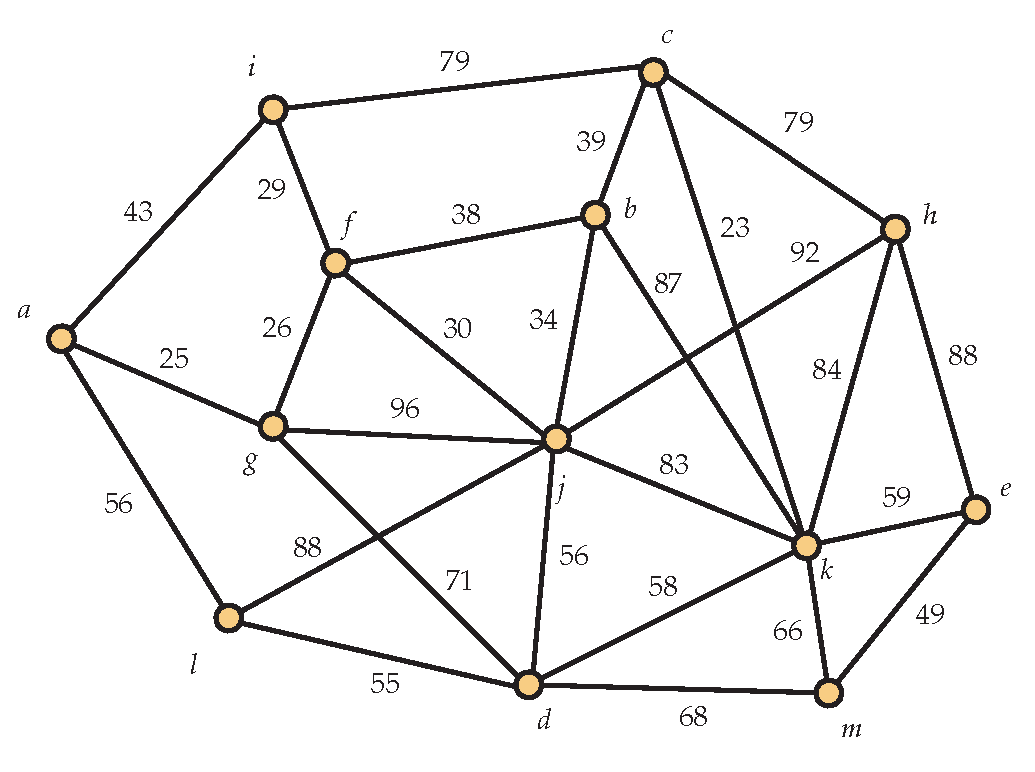
\includegraphics[width=3.5in]{graphalgorithms-figs/spantreegraph}
\caption{\label{fig:graphalgorithms:spantreegraph}A weighted graph}
\end{center}
\end{figure}
To do this, this section considers the following problem:
\begin{problem*}
   Find a minimum weight spanning tree $\bfT$ of $\bfG$.
\end{problem*}
To solve this problem, we will develop \textit{two} efficient graph
algorithms, each having certain computational advantages and
disadvantages. Before developing the algorithms, we need to establish
some preliminaries about spanning trees and forests.

\subsection{Preliminaries}

The following proposition about the number of components in a spanning
forest of a graph $\bfG$ has an easy inductive proof. You are asked to
provide it in the exercises.

\begin{proposition}\label{prop:graphalgorithms:spanforest}
Let $\GVE$ be a graph on $n$ vertices, and let $\bfH=(V,S)$ be
a spanning forest.  Then $0\le |S|\le n-1$.  Futhermore, if
$|S|= n-k$, then $\bfH$ has $k$ components.  In particular, $\bfH$ is
a spanning tree if and only if it contains $n-1$ edges.
\end{proposition}

The following proposition establishes a way to take a spanning tree of
a graph, remove an edge from it, and add an edge of the graph that is
not in the spanning tree to create a new spanning tree. Effectively,
the process exchanges two edges to form the new spanning tree, so we
call this the \emph{exchange principle}.

\begin{proposition}[Exchange Principle]\label{prop:graphalgorithms:exchange}
Let $\bfT=(V,S)$ be spanning tree in a graph $\bfG$, and let $e=xy$ be
an edge of $\bfG$ which does not belong to $\bfT$.  Then
\begin{enumerate}
\item  There is a \emph{unique} path $P=(x_0,x_1,x_2,\dots,x_t)$
with (a)~$x=x_0$; (b)~$y=x_t$; and (c)~$x_ix_{i+1}\in S$ for each
$i=0,1,2,\dots,t-1$.
\item  For each $i=0,1,2,\dots,t-1$, let $f_i=x_ix_{i+1}$ and 
  then set \[S_i = \{e\}\cup\{g\in S: g\neq f_i\},\] i.e., we \emph{exchange}
edge $f_i$ for edge $e$. Then $\bfT_i=(V,S_i)$ is a spanning tree of $\bfG$.
\end{enumerate}
\end{proposition}

\begin{proof}
  For the first fact, it suffices to note that if there were more than
  one distinct path from $x$ to $y$ in $\bfT$, we would be able to
  find a cycle in $\bfT$. This is impossible since it is a tree. For
  the second, we refer to \autoref{fig:graphalgorithms:exchange}. The
  black and green edges in the graph shown at the left represent the
  spanning tree $\bfT$. Thus, $f$ lies on the unique path from $x$ to
  $y$ in $\bfT$ and $e=xy$ is an edge of $\bfG$ \emph{not} in
  $\bfT$. Adding $e$ to $\bfT$ creates a graph with a unique cycle,
  since $\bfT$ had a unique path from $x$ to $y$. Removing $f$ (which
  could be any edge $f_i$ of the path, as stated in the proposition)
  destroys this cycle. Thus $\bfT_i$ is an acyclic subgraph of $\bfG$
  with $n-1+1-1=n-1$ edges, so it is a spanning tree.
  \begin{figure}[h]
    \centering
    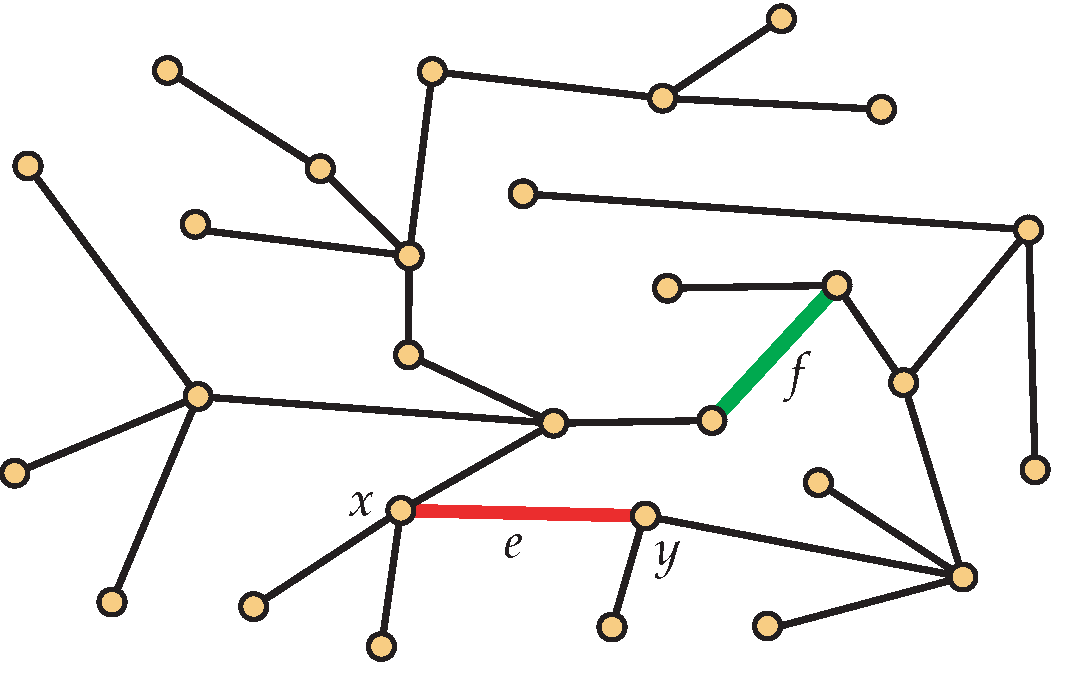
\includegraphics[width=0.45\linewidth]{graphalgorithms-figs/exchange1}\hspace{0.05\linewidth}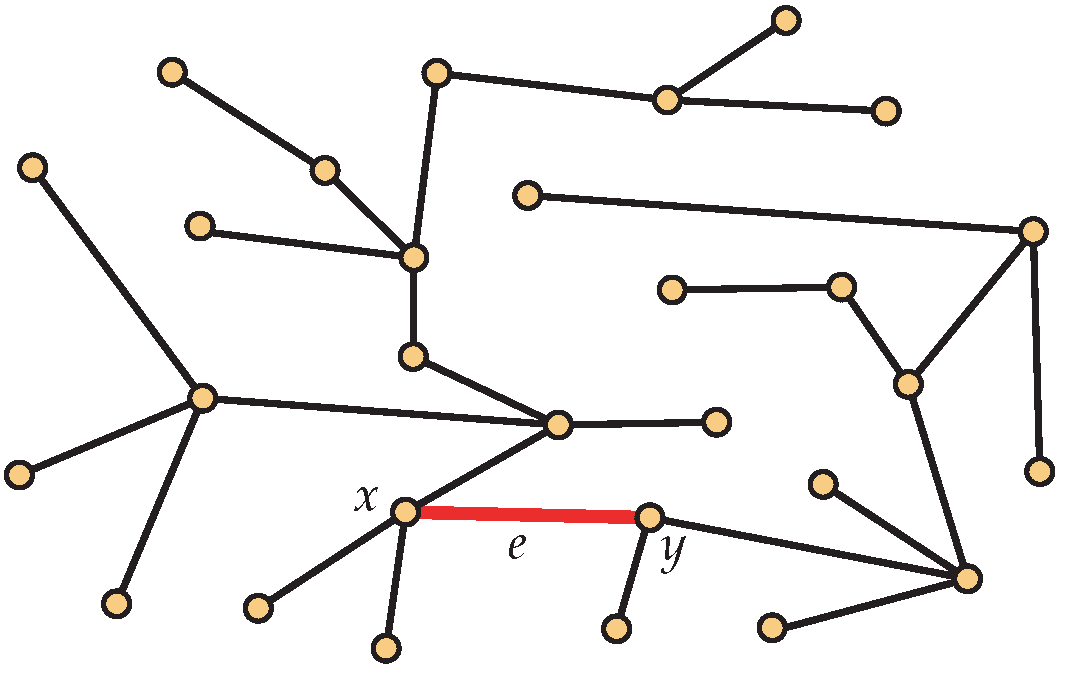
\includegraphics[width=0.45\linewidth]{graphalgorithms-figs/exchange2}
    \caption{The exchange principle}
    \label{fig:graphalgorithms:exchange}
  \end{figure}
\end{proof}
 
For both of the algorithms we develop, the argument to show that the
algorithm is optimal rests on the following technical lemma.  To avoid
trivialities, we assume $n\ge3$.

\begin{lemma}\label{lem:graphalgorithms:tech}
  Let $\bfF$ be a spanning forest of $\bfG$ and let $C$ be a component
  of $\bfF$.  Also, let $e=xy$ be an edge of minimum weight among all
  edges with one endpoint in $C$ and the other not in $C$.  Then among
  all spanning trees of $\bfG$ that contain the forest $\bfF$, there
  is one of minimum weight that contains the edge $e$.
\end{lemma}
\begin{proof}
  Let $\bfT=(V,S)$ be any spanning tree of minimum weight among all
  spanning trees that contain the forest $\bfF$, and suppose that
  $e=xy$ is not an edge in $\bfT$. (If it were an edge in $\bfT$, we
  would be done.) Then let $P=(x_0,x_1,x_2,\dots,x_t)$ be the unique
  path in $\bfT$ with (a)~$x=x_0$; (b)~$y=x_t$; and (c)~$x_ix_{i+1}\in
  S$ for each $i=0,1,2,\dots,t-1$.  Without loss of generality, we may
  assume that $x=x_0$ is a vertex in $C$ while $y=x_t$ does not
  belong to $C$.  Then there is a
  least non-negative integer $i$ for which $x_i$ is in $C$ and
  $x_{i+1}$ is not in $C$.  It follows that $x_j$ is in $C$ for all $j$ with
  $0\le j\le i$.

  Let $f=x_ix_{i+1}$. The edge $e$ has minimum weight among all edges
  with one endpoint in $C$ and the other not in $C$, so $w(e)\le
  w(f)$.  Now let $\bfT_i$ be the tree obtained by exchanging the edge
  $f$ for edge~$e$.  It follows that $w(\bfT_i) = w(\bfT) - w(f)
  +w(e)\le w(\bfT)$.  Furthermore, $\bfT_i$ contains the spanning
  forest $\bfF$ as well as the edge~$e$. It is therefore the minimum
  weight spanning tree we seek.
\end{proof}

\section{Discussion}
  Although Bob's combinatorial intuition has improved over the course
  he doesn't quite understand why we need
  special algorithms to find minimum weight spanning trees. He figures
  there can't be that many spanning trees, so he wants to just write
  them down. Alice groans as she senses that Bob must have
  been absent when the material from 
  \autoref{s:graphs:counting-trees}  was discussed.  In that section,
  we learned that a graph on $n$ vertices can have as many as $n^{n-2}$
  spanning trees (or horrors, the instructor may have left it off the
  syllabus).  Regardless, this exhaustive approach is already unusable
  when $n = 20$. Dave mumbles something about being greedy and just adding the
  lightest edges one-by-one while never adding an edge that would make
  a cycle. Zori remembers a strategy like this working for finding
  the height of a poset, but she's worried about the nightmare
  situation that we learned about with using FirstFit to color
  graphs. Alice agrees that greedy algorithms have an inconsistent
  track record but suggests that
  \hyperref[lem:graphalgorithms:tech]{Lemma~\ref*{lem:graphalgorithms:tech}}
  may be enough to get one to succeed here.

\subsection{Kruskal's Algorithm}

In this secton, we develop one of the best known algorithms for
finding a minimum weight spanning tree.  It is known as Kruskal's
Algorithm, although some prefer the descriptive label \textit{Avoid
  Cycles} because of the way it builds the spanning tree.

To start Kruskal's algorithm, we sort the edges according to weight.
To be more precise, let $m$ denote the number of edges in $\GVE$.
Then label the edges as $e_1,e_2,e_3,\dots,e_m$ so that $w(e_1)\le
w(e_2)\le \dots \le w(e_m)$. Any of the many available efficient
sorting algorithms can be used to do this step.

Once the edges are sorted, Kruskal's algorithm proceeds to an
initialization step and then inductively builds the spanning tree
$\bfT=(V,S)$:

\medskip
\textbf{Initialization.}\quad
Set $S=\emptyset$ and $i=0$.

\medskip
\textbf{Inductive Step.}\quad
While $|S| < n-1$, let $j$ be the least non-negative
integer so that $j > i$ and there are no cycles in
$S\cup\{e_j\}$.  Then (using pseudo-code) set
\[
i = j\quad\text{and}\quad S= S\cup\{j\}.
\]

The correctness of Kruskal's Algorithm follows from an inductive
argument. First, the set $S$ is initialized as the empty set, so there
is certainly a minimum weight spanning tree containing all the edges
in $S$.  Now suppose that for some $i$ with $0\le i <n$, $|S|=i$ and
there is a minimum weight spanning tree containing all the edges in
$S$.  Let $\bfF$ be the spanning forest determined by the edges in
$S$, and let $C_1, C_2,\dots,C_s$ be the components of $\bfF$.  For
each $k=1,2,\dots,s$, let $f_k$ be a minimum weight edge with one
endpoint in $C_k$ and the other not in $C_k$.  Then the edge $e$ added
to $S$ by Kruskal's Algorithm is just the edge $\{f_1,f_2,\dots,f_s\}$
having minimum weight. Applying
\hyperref[lem:graphalgorithms:tech]{Lemma~\ref*{lem:graphalgorithms:tech}}
and the inductive hypothesis, we know that there will still be a
minimum weight spanning tree of $\bfG$ containing all the edges of
$S\cup\{e\}$.

\medskip
\noindent\begin{minipage}{0.70\textwidth}
\begin{example}
  Let's see what Kruskal's algorithm does on the weighted graph in
  \autoref{fig:graphalgorithms:spantreegraph}. It first sorts all of
  the edges by weight. We won't reproduce the list here, since we
  won't need all of it. The edge of least weight is $ck$, which has
  weight $23$. It continues adding the edge of least weight, adding
  $ag$, $fg$, $fi$, $fj$, and $bj$. However, after doing this, the
  edge of lowest weight is $fb$, which has weight $38$. This edge
  cannot be added, as doing so would make $fjb$ a cycle. Thus, the
  algorithm bypasses it and adds $bc$. Edge $ai$ is next inspected,
  but it, too, would create a cycle and is eliminated from
  consideration. Then $em$ is added, followed by $dl$. There are now
  \emph{two} edges of weight $56$ to be considered: $al$ and $dj$. Our
  sorting algorithm has somehow decided one of them should appear
  first, so let's say it's $dj$. After adding $dj$, we cannot add
  $al$, as $agfjdl$ would form a cycle. Edge $dk$ is next considered,
  but it would also form a cycle. However, $ek$ can be added. Edges
  $km$ and $dm$ are then bypassed. Finally, edge $ch$ is added as the
  twelfth and final edge for this $13$-vertex spanning tree. The full
  list of edges added (in order) is shown to the right. The total
  weight of this spanning tree is $504$.\end{example}
\end{minipage}\hspace{.03\textwidth}
\begin{minipage}{.25\textwidth}
\begin{center}\textbf{Kruskal's Algorithm}\\%
  \begin{tt}c k 23\\%
     a g 25\\%
     f g 26\\%
     f i 29\\%
     f j 30\\%
     b j 34\\%
     b c 39\\%
     e m 49\\%
     d l 55\\%
     d j 56\\%
     e k 59\\%
     c h 79\end{tt}\end{center}\end{minipage}
\subsection{Prim's Algorithm}

We now develop Prim's Algorithm for finding a minimum weight spanning
tree. This algorithm is also known by a more descriptive label:
\textit{Build Tree}.  We begin by choosing a root vertex $r$. Again,
the algorithm proceeds with an initialization step followed by a
series of inductive steps.

\medskip
\textbf{Initialization.}\quad
Set $W=\{r\}$ and $S=\emptyset$.

\medskip
\textbf{Inductive Step.}\quad
While $|W| < n$, let $e$ be an edge of minimum weight among
all edges with one endpoint in $W$ and the other not in $W$.
If $e=xy$, $x\in W$ and $y\not\in W$, update $W$ and $S$ by
setting (using pseudo-code)
\[
W = W\cup\{y\}\quad\text{and}\quad S = S\cup\{e\}.
\]

The correctness of Prim's algorithm follows immediately from
\hyperref[lem:graphalgorithms:tech]{Lemma~\ref*{lem:graphalgorithms:tech}}.

\medskip
\noindent\begin{minipage}{0.70\textwidth}
\begin{example}
  Let's see what Prim's algorithm does on the weighted graph in
  \autoref{fig:graphalgorithms:spantreegraph}. We start with vertex
  $a$ as the root vertex. The lightest edge connecting $a$ (the only
  vertex in the tree so far) to the rest of the graph is $ag$. Next,
  $fg$ is added. This is followed by $fi$, $fj$, $bj$, and $bc$. Next,
  the algorithm identifies $ck$ as the lightest edge connecting
  $\{a,g,i,f,j,b,c\}$ to the remaining vertices. Notice that this is
  considerably later than Kruskal's algorithm finds the same edge. The
  algorithm then determines that $al$ and $jd$, both of weight $56$
  are the lightest edges connecting vertices in the tree to the other
  vertices. It picks arbitrarily, so let's say it takes $al$. It next
  finds $dl$, then $ek$, and then $em$. The final edge added is $ch$. The full
  list of edges added (in order) is shown to the right. The total
  weight of this spanning tree is $504$. This (not surprisingly) the
  same weight we obtained using Kruskal's algorithm. However, notice
  that the spanning tree found is different, as this one contains
  $al$ instead of $dj$. This is not an issue, of course, since in
  both cases an arbitrary choice between two edges of equal weight
  was made.\end{example}
\end{minipage}\hspace{.03\textwidth}
\begin{minipage}{.25\textwidth}
\begin{center}\textbf{Prim's Algorithm}\\

\medskip
\begin{tt}
a g 25\\
f g 26\\
f i 29\\
f j 30\\
b j 34\\
b c 39\\
c k 23\\
a l 56\\
d l 55\\
e k 59\\
e m 49\\
c h 79
\end{tt}\end{center}\end{minipage}

\subsection{Comments on Efficiency}

An implementation of Kruskal's algorithm seems to require that
the edges be sorted.  If the graph has $n$ vertices and $m$  edges,
this requires $m\log m$ operations just for the sort.  But once
the sort is done, the process takes only $n-1$ steps---provided
you keep track of the components as the spanning forest expands.
Regardless, it is easy to see that at most $O(n^2\log n)$ operations
are required.

On the other hand, an implementation of Prim's algorithm requires
the program to conveniently keep track of the edges incident with
each vertex and always be able to identify the edge with least
weight among subsets of these edges.  In computer science, the
data structure that enables this task to be carried out is called
a \textit{heap}.

\section{Digraphs}

In this section, we introduce another useful variant of a graph. In a
graph, the existence of an edge $xy$ can be used to model a connection
between $x$ and $y$ that goes in both ways. However, sometimes such a
model is insufficient. For instance, perhaps it is possible to fly
from Atlanta directly to Fargo but not possible to fly from Fargo
directly to Atlanta. In a graph representing the airline network, an
edge between Atlanta and Fargo would lose the information that the
flights only operate in one direction. To deal with this problem, we
introduce a new discrete structure. A \textit{digraph} $\bfG$ is a
pair $(V,E)$ where $V$ is a vertex set and $E\subset V\times V$ with
$x\neq y$ for every $(x,y)\in E$.  We consider the pair $(x,y)$ as a
\textit{directed edge} from $x$ to $y$.  Note that for distinct
vertices $x$ and $y$ from $V$, the ordered pairs $(x,y)$ and $(y,x)$
are distinct, so the digraph may have one, both or neither of the
directed edges $(x,y)$ and $(y,x)$. This is in contrast to graphs,
where edges are sets, so $\{x,y\}$ and $\{y,x\}$ are the same.

Diagrams of digraphs use arrowheads on the edges to indicate direction.
This is illustrated in \autoref{fig:graphalgorithms:digraph}. For
example, the digraph illustrated there contains the edge $(a,f)$ but
not the edge $(f,a)$. It does contain both edges $(c,d)$ and $(d,c)$,
however.

\begin{figure}[t]
\begin{center}
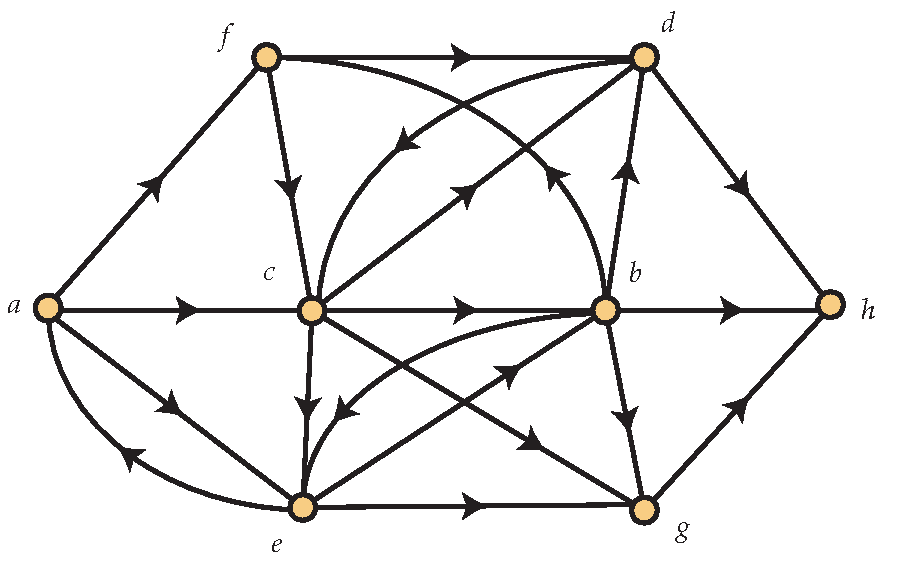
\includegraphics[width=3in]{graphalgorithms-figs/digraph}\\
\caption{A Digraph}
\label{fig:graphalgorithms:digraph}
\end{center}
\end{figure}

When $\bfG$ is a digraph, a sequence $P=(r=u_0,u_1,\dots,u_t=x)$ of
distinct vertices is called a \textit{directed path} from $r$ to $x$
when $(u_iu_{i+1})$ is a directed edge in $\bfG$ for every
$i=0,1,\dots,t-1$.  A directed path $C=(r=u_0,u_1,\dots,u_t=x)$ is
called a \textit{directed cycle} when $(u_t,u_0)$ is a directed edge
of $\bfG$.

\section{Dijkstra's Algorithm for Shortest Paths}

Just as with graphs, it is useful to assign weights to the directed
edges of a digraph. Specifically, in this section we consider a pair
$(\bfG,w)$ where $\GVE$ is a digraph and $w:E\rightarrow\mathbb{N}_0$
is a function assigning to each directed edge $(x,y)$ a non-negative
weight $w(x,y)$.  However, in this section, we interpret weight as
\textit{distance} so that $w(x,y)$ is now called the \textit{length}
of the edge $(x,y)$.  If $P=(r=u_0,u_1,\dots,u_t=x)$ is a directed
path from $r$ to $x$, then the \textit{length} of the path $P$ is just
the sum of the lengths of the edges in the path, $\sum_{i=0}^{t-1}
w(u_iu_{i+1})$.  The \textit{distance} from $r$ to $x$ is then defined
to be the minimum length of a directed path from $r$ to $x$. Our goal
in this section is to solve the following natural problem, which has
many applications:

\medskip
\noindent\textbf{Problem.}\quad
For each vertex $x$, find the distance from $r$ to $x$.  Also, find a
shortest path from $r$ to $x$.

\subsection{Description of the Algorithm}

To describe Dijkstra's algorithm in a compact manner, it is useful to
extend the definition of the function $w$. We do this by by setting
$w(x,y)=\infty$ when $x\neq y$ and $(x,y)$ is not a directed edge of
$\bfG$. In this way, we will treat $\infty$ as if it were a number
(although it is not!).\footnote{This is not an issue for computer
  implementation of the algorithm, as instead of using $\infty$, a
  value given by the product of the number of vertices and the 
  maximum edge weight may be used to simulate infinity.} 

Let $n=|V|$.  At Step~$i$, where $1\le i\le n$, we will 
have determined: 
\begin{enumerate}
\item A sequence $\sigma=(v_1,v_2,v_3,\dots,v_i)$ of distinct 
vertices from $\bfG$ with $r=v_1$.  These vertices are called 
\textit{permanent} vertices, while the remaining vertices will
be called \textit{temporary} vertices.
\item For each vertex $x\in V$, we will have determined a
  number $\delta(x)$ and a path $P(x)$ from $r$ to $x$ of
  length $\delta(x)$.
\end{enumerate}

\noindent\textbf{Initialization} (Step 1).\quad
Set $i=1$. Set $\delta(r)=0$ and let $P(r)=(r)$ be the trivial
one-point path.  Also, set $\sigma= (r)$.  For each $x\neq r$, set
$\delta(x)= w(r,x)$ and $P(x)=(r,x)$. Let $x$ be a temporary vertex
for which $\delta(x)$ is minimum. Set $v_2 = x$, and update $\sigma$
by appending $v_2$ to the end of it. Increment $i$.

\medskip
\noindent\textbf{Inductive Step} (Step $i$, $i>1$).\quad
If $i<n$, then
for each temporary $x$, let
\[\delta(x) = \min\{\delta(x), \delta(v_i)+w(v_i,x)\}.\]
If this assignment results in a reduction in the
value of $\delta(x)$, let $P(x)$ be the
path obtained by adding $x$ to the end of $P(v_i)$.

Let $x$ be a temporary vertex for which $\delta(x)$ is minimum.  Set
$v_{i+1}=x$, and update $\sigma$ by appending $v_{i+1}$ to
it. Increment $i$.

\subsection{Example}

Before establishing why Dijkstra's algorithm works, it may be helpful
to see an example of how it works. To do this, consider the digraph
$\bfG$ shown in \autoref{fig:graphalgorithms:dijkstragraph}.  For
visual clarity, we have chosen a digraph which is an \textit{oriented
  graph}, i.e., for each distinct pair $x,y$ of vertices, the graph
contains at most one of the two possible directed edges $(x,y)$ and
$(y,x)$.

\begin{figure}[t]
\begin{center}
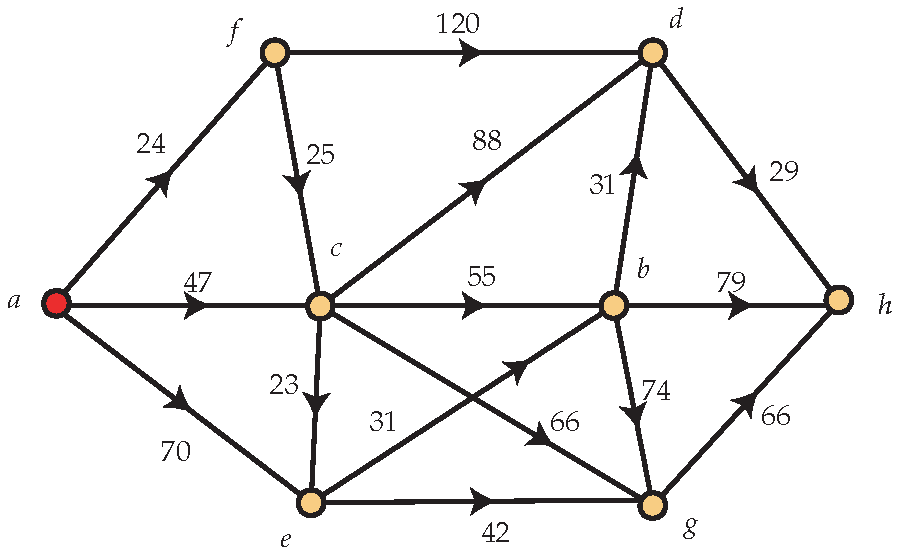
\includegraphics[width=3in]{graphalgorithms-figs/dijkstragraph}\\
\caption{A digraph with edge lengths}
\label{fig:graphalgorithms:dijkstragraph}
\end{center}
\end{figure}

Suppose that the root vertex $r$ is the vertex labeled~$a$. The
initialization step of Dijkstra's algorithm then results in the
following values for $\delta$ and $P$:

\textbf{Initialization (Step 1)}

\begingroup
\leftskip25pt
\rightskip\leftskip

\medskip
$\sigma=(a)$\\
$\delta(a)=0$; $P(a)=(a)$\\
$\delta(b)=\infty$; $P(b)=(a,b)$\\
$\delta(c)=47$; $P(c)=(a,c)$\\
$\delta(d)=\infty$; $P(d)=(a,d)$\\
$\delta(e)=70$; $P(e)=(a,e)$\\
$\delta(f)=24$; $P(f)=(a,f)$\\
$\delta(g)=\infty$; $P(g)=(a,g)$\\
$\delta(h)=\infty$; $P(h)=(a,h)$\\

\endgroup

Before finishing Step 1, the algorithm identifies vertex~$f$ as
closest to $a$ and appends it to $\sigma$, making $a$ permanent. When
entering Step 2, Dijkstra's algorithm attempts to find shorter paths
from $a$ to each of the temporary vertices by going through $f$. We
call this process ``scanning from vertex~$f$.'' In this scan, the path
to vertex~$d$ is updated, since $\delta(f) + w(f,d)=24+120=144<
\infty=w(a,d)$.

\medskip
\textbf{Step 2.}\quad Scan from vertex~$f$.

\begingroup
\leftskip25pt
\rightskip\leftskip

\medskip
$\sigma=(a,f)$\\
$\delta(a)=0$; $P(a)=(a)$\\
$\delta(b)=\infty$; $P(b)=(a,b)$\\
$\delta(c)=47$; $P(c)=(a,c)$\\
$\delta(d)=144 = 24 + 120 = \delta(f)+w(f,d)$; $P(d)=(a,f,d)$\quad\text{updated}\\
$\delta(e)=70$; $P(e)=(a,e)$\\
$\delta(f)=24$; $P(f)=(a,f)$\\
$\delta(g)=\infty$; $P(g)=(a,f)$\\
$\delta(h)=\infty$; $P(h)=(a,h)$\\

\endgroup

Before proceeding to the next step, vertex~$c$ is made permanent by
making it $v_3$. In Step 3, therefore, the scan is from vertex
$c$. Vertices $b$, $d$, and $g$ have their paths updated. However,
although $\delta(c) + w(c,e) = 47+23=70=\delta(e)$, we do not
change $P(e)$ since $\delta(e)$ is not \emph{decreased} by routing
$P(e)$ through $c$.

\medskip
\textbf{Step 3.}\quad Scan from vertex~$c$.

\begingroup
\leftskip25pt
\rightskip\leftskip

\medskip
$\sigma=(a,f,c)$\\
$\delta(a)=0$; $P(a)=(a)$\\
$\delta(b)=102=47+55= \delta(c)+w(c,b)$; $P(b)=(a,c,b)$\quad\text{updated}\\
$\delta(c)=47$; $P(c)=(a,c)$\\
$\delta(d)=135=47+88 = \delta(c)+w(c,d)$; $P(d)=(a,c,d)$\quad\text{updated}\\
$\delta(e)=70$; $P(e)=(a,e)$\\
$\delta(f)=24$; $P(f)=(a,f)$\\
$\delta(g)=113=47+66= \delta(c)+w(c,g)$; $P(g)=(a,c,g)$\quad\text{updated}\\
$\delta(h)=\infty$; $P(h)=(a,h)$\\

\endgroup

Now vertex $e$ is made permanent.

\medskip
\textbf{Step 4.}\quad Scan from vertex~$e$.

\begingroup
\leftskip25pt
\rightskip\leftskip

\medskip
$\sigma=(a,f,c,e)$\\
$\delta(a)=0$; $P(a)=(a)$\\
$\delta(b)=101=70+31= \delta(e)+w(e,b)$; $P(b)=(a,e,b)$\quad\text{updated}\\
$\delta(c)=47$; $P(c)=(a,c)$\\
$\delta(d)=135$; $P(d)=(a,c,d)$\\
$\delta(e)=70$; $P(e)=(a,e)$\\
$\delta(f)=24$; $P(f)=(a,f)$\\
$\delta(g)=112=70+42= \delta(e)+w(e,g)$; $P(g)=(a,e,g)$\quad\text{updated}\\
$\delta(h)=\infty$; $P(h)=(a,h)$\\

\endgroup

Now vertex $b$ is made permanent.

\medskip
\textbf{Step 5.}\quad Scan from vertex~$b$.

\begingroup
\leftskip25pt
\rightskip\leftskip

\medskip
$\sigma=(a,f,c,e,b)$\\
$\delta(a)=0$; $P(a)=(a)$\\
$\delta(b)=101$; $P(b)=(a,e,b)$\\
$\delta(c)=47$; $P(c)=(a,c)$\\
$\delta(d)= 132 = 101+ 31= \delta(b)+w(b,d)$; $P(d)=(a,e,b,d)$\quad\text{updated}\\
$\delta(e)= 70$; $P(e)=(a,e)$\\
$\delta(f)= 24$; $P(f)=(a,f)$\\
$\delta(g)=112$; $P(g)=(a,e,g)$\\
$\delta(h)=180 = 101+79=\delta(b)+w(b,h)$; $P(h)=(a,e,b,h)$\quad\text{updated}\\

\endgroup

Now vertex $g$ is made permanent.

\medskip
\textbf{Step 6.}\quad Scan from vertex~$g$.

\begingroup
\leftskip25pt
\rightskip\leftskip

\medskip
$\sigma=(a,f,c,e,b,g)$\\
$\delta(a)=0$; $P(a)=(a)$\\
$\delta(b)=101$; $P(b)=(a,e,b)$\\
$\delta(c)=47$; $P(c)=(a,c)$\\
$\delta(d)= 132$; $P(d)=(a,e,b,d)$\\
$\delta(e)=70$; $P(e)=(a,e)$\\
$\delta(f)=24$; $P(f)=(a,f)$\\
$\delta(g)=112$; $P(g)=(a,e,g)$\\
$\delta(h)=178 = 112+66=\delta(g)+w(g,h)$; $P(h)=(a,e,g,h)$\quad\text{updated}\\

\endgroup

Now vertex $d$ is made permanent.

\medskip
\textbf{Step 7.}\quad Scan from vertex~$d$.

\begingroup
\leftskip25pt
\rightskip\leftskip

\medskip
$\sigma=(a,f,c,e,b,g,d)$\\
$\delta(a)=0$; $P(a)=(a)$\\
$\delta(b)=101$; $P(b)=(a,e,b)$\\
$\delta(c)=47$; $P(c)=(a,c)$\\
$\delta(d)= 132$; $P(d)=(a,e,b,d)$\\
$\delta(e)=70$; $P(e)=(a,e)$\\
$\delta(f)=24$; $P(f)=(a,f)$\\
$\delta(g)=112$; $P(g)=(a,e,g)$\\
$\delta(h)=161 = 132+29=\delta(d)+w(d,h)$; $P(h)=(a,e,b,d,h)$\quad\text{updated}\\

\endgroup

Now vertex $h$ is made permanent. Since this is the last vertex, the
algorithm halts and returns the following:

\medskip
\textbf{FINAL RESULTS}\quad 

\begingroup
\leftskip25pt
\rightskip\leftskip

\medskip
$\sigma=(a,f,c,e,b,g,d,h)$\\
$\delta(a)=0$; $P(a)=(a)$\\
$\delta(b)=101$; $P(b)=(a,e,b)$\\
$\delta(c)=47$; $P(c)=(a,c)$\\
$\delta(d)= 132$; $P(d)=(a,e,b,d)$\\
$\delta(e)=70$; $P(e)=(a,e)$\\
$\delta(f)=24$; $P(f)=(a,f)$\\
$\delta(g)=112$; $P(g)=(a,e,g)$\\
$\delta(h)=161$; $P(h)=(a,e,b,d,h)$\\

\endgroup

\subsection{The Correctness of Dijkstra's Algorithm}

Now that we've illustrated Dijkstra's algorithm, it's time to prove
that it actually does what we claimed it does: find the distance from
the root vertex to each of the other vertices and a path of that
length. To do this, we first state two elementary propositions. The
first is about shortest paths in general, while the second is specific
to the sequence of permanent vertices produced by Dijkstra's algorithm.

\begin{proposition}
Let $x$ be a vertex and let $P=(r=u_0,u_1,\dots,u_t=x)$ be
a shortest path from $r$ to $x$.  Then for every
integer $j$ with $0<j<t$,
$(u_0,u_1,\dots,u_j)$ is a shortest path from $r$
to $u_j$ and $(u_j,u_{j+1},\dots,u_t)$ is a shortest
path from $u_j$ to $u_t$
\end{proposition}

\begin{proposition}
When the algorithm halts, let $\sigma=(v_1,v_2,v_3,\dots,v_n)$. 
Then \[\delta(v_1)\le \delta(v_2)\le\dots \le \delta(v_n). \]
\end{proposition}

We are now ready to prove the correctness of the algorithm. The proof
we give will be inductive, but the induction will have nothing to do
with the total number of vertices in the digraph or the step number
the algorithm is in.

\begin{theorem}
  Dijkstra's algorithm yields shortest paths for every vertex $x$ in
  $\bfG$. That is, when Dijkstra's algorithm terminates, for each
  $x\in V$, the value $\delta(x)$ is the distance from $r$ to $x$ and
  $P(x)$ is a shortest path from $r$ to $x$.
\end{theorem}

\begin{proof}
  The theorem holds trivially when $x=r$.  So we consider the case
  where $x\neq r$.  We argue that $\delta(x)$ is the distance from $r$
  to $x$ and that $P(x)$ is a shortest path from $r$ to $x$ by
  induction on the minimum number $k$ of edges in a shortest path from
  $r$ to $x$. When $k=1$, the edge $(r,x)$ is a shortest path from $r$
  to $x$.  Since $v_1=r$, we will set $\delta(x)=w(r,x)$ and
  $P(x)=(r,x)$ at Step~1.

  Now fix a positive integer $k$. Assume that if the minimum number of
  edges in a shortest path from $r$ to $x$ is at most $k$, then
  $\delta(x)$ is the distance from $r$ to $x$ and $P(x)$ is a shortest
  path from $r$ to $x$. Let $x$ be a vertex for which the minimum
  number of edges in a shortest path from $r$ to $x$ is $k+1$.  Fix a
  a shortest path $P=(u_0,u_1,u_2,\dots,u_{k+1})$ from $r=u_0$ to
  $x=u_{k+1}$.  Then $Q=(u_0,u_1,\dots,u_k)$ is a shortest path from
  $r$ to $u_k$. (See \autoref{fig:graphalgorithms:dijkstra-proof}.)

  \begin{figure}[b]
    \centering
    \begin{overpic}[width=0.6\textwidth]{graphalgorithms-figs/dijkstra-proof}
      \put(3,13){$r$}
      \put(33,25){$Q$}
      \put(58,3){$P(u_k)$}
      \put(73,28){$u_k$}
      \put(83,25){$P$}
      \put(93,21){$x$}
    \end{overpic}
    \caption{Shortest paths}
    \label{fig:graphalgorithms:dijkstra-proof}
  \end{figure}

  By the inductive hypothesis, $\delta(u_k)$ is the distance from $r$
  to $u_k$, and $P(u_k)$ is a shortest path from $r$ to $u_k$.  Note
  that $P(u_k)$ need not be the same as path $Q$, as we suggest in
  \autoref{fig:graphalgorithms:dijkstra-proof}.  However, if distinct,
  the two paths will have the same length, namely $\delta(u_k)$.
  Also, the distance from $r$ to $x$ is $\delta(u_k)+w(u_k,x)\ge
  \delta(u_k)$ since $P$ is a shortest path from $r$ to $x$ and
  $w(u_k,x)\geq 0$.

  Let $i$ and $j$ be the unique integers for which $u_k=v_i$ and
  $x=v_j$.  If $j < i$, then
  \[
  \delta(x)= \delta(v_j)\le \delta(v_i)= \delta(u_k)\le
  \delta(u_k)+w(u_k).
  \]
  Therefore the algorithm has found a path $P(x)$ from $r$ to $x$
  having length $\delta(x)$ which is at most the distance from $r$ to
  $x$.  Clearly, this implies that $\delta(x)$ is the distance from
  $r$ to $x$ and that $P(x)$ is a shortest path.

  On the other hand, if $j>i$, then the inductive step at Step~$i$
  results in
  \[
  \delta(x)\le \delta(v_i)+w(v_i,y)=\delta(u_k)+w(u_k,x).
  \]
  As before, this implies that $\delta(x)$ is the distance from $r$ to
  $x$ and that $P(x)$ is a shortest path.
\end{proof}


\section{Historical Notes}

Kruskal's algorithm was published in 1956 by Joseph B.\ Kruskal in a
three-page paper that appeared in \emph{Proceedings of the American
  Mathematical Society}. Robert C.\ Prim published the algorithm that
now bears his name the following year in \emph{The Bell System
  Technical Journal}. Prim's paper focuses on application of the
minimum weight (or length or cost) spanning tree problem to telephone
networks. He was aware of Kruskal's prior work, as they were
colleagues at Bell Laboratories at the time he published his paper. It
turns out that Prim had been beaten to the punch by Czech
mathematician Vojt\v{e}ch Jarn\'{i}k in 1929, so some refer to Prim's
algorithm as Jarn\'{i}k's algorithm. (It was later rediscovered by
Dijkstra, so some attach his name as well, referring to it as the
Dijkstra-Jarn\'{i}k-Prim algorithm.) Edsger Dijkstra published his
algorithm for finding shortest paths in 1959 in a three-page
paper\footnote{This is also the paper in which Prim's algorithm was
  published for the third time. Dijkstra was aware of Kruskal's prior
  work but argued that his algorithm was preferable because it
  required that less information about the graph be stored in memory
  at each step of the algorithm.}  appearing in \emph{Numerische
  Mathematik}. In fact, Dijkstra's algorithm had been discovered (in
an equivalent form) by Edward F.\ Moore two years earlier. His result
appeared in \emph{Proceedings of an International Symposium on the
  Theory of Switching}.

\section{Exercises}

\begin{enumerate}
\item For the graph in \autoref{fig:span_tree_ex1}, use Kruskal's
  algorithm (``avoid cycles'') to find a minimum weight spanning
  tree. Your answer should include a complete list of the edges,
  indicating which edges you take for your tree and which (if any) you
  reject in the course of running the algorithm.
  \begin{figure}[h]
    \centering
    \includegraphics[scale=0.65]{graphalgorithms-figs/span_tree_ex1}
    \caption{Find a minimum weight spanning tree}
    \label{fig:span_tree_ex1}
  \end{figure}
\item For the graph in \autoref{fig:span_tree_ex1}, use Prim's
  algorithm (``build tree'') to find a minimum weight spanning
  tree. Your answer should list the edges selected by the algorithm in
  the order they were selected.
\item For the graph in \autoref{fig:span_tree_ex2}, use Kruskal's
  algorithm (``avoid cycles'') to find a minimum weight spanning
  tree. Your answer should include a complete list of the edges,
  indicating which edges you take for your tree and which (if any) you
  reject in the course of running the algorithm.
  \begin{figure}[h]
    \centering
    \includegraphics[scale=0.65]{graphalgorithms-figs/span_tree_ex2}
    \caption{Find a minimum weight spanning tree}
    \label{fig:span_tree_ex2}
  \end{figure}
\item For the graph in \autoref{fig:span_tree_ex2}, use Prim's
  algorithm (``build tree'') to find a minimum weight spanning
  tree. Your answer should list the edges selected by the algorithm in
  the order they were selected.
\item For the graph in \autoref{fig:span_tree_ex3}, use Kruskal's
  algorithm (``avoid cycles'') to find a minimum weight spanning
  tree. Your answer should include a complete list of the edges,
  indicating which edges you take for your tree and which (if any) you
  reject in the course of running the algorithm.
  \begin{figure}[h]
    \centering
    \includegraphics[scale=0.65]{graphalgorithms-figs/span_tree_ex3}
    \caption{Find a minimum weight spanning tree}
    \label{fig:span_tree_ex3}
  \end{figure}
\item For the graph in \autoref{fig:span_tree_ex3}, use Prim's
  algorithm (``build tree'') to find a minimum weight spanning
  tree. Your answer should list the edges selected by the algorithm in
  the order they were selected.
\item A new local bank is being created and will establish a
  headquarters $h$, two branches $b_1$ and $b_2$, and four ATMs $a_1$,
  $a_2$, $a_3$, and $a_4$. They need to build a computer network such
  that the headquarters, branches, and ATMs can all
  intercommunicate. Furthermore, they will need to be networked with
  the Federal Reserve Bank of Atlanta, $f$. The costs of the feasible
  network connections (in units of \$10,000) are listed below:
  \begin{align*}
    h f & \quad 80 &
    h b_1 & \quad 10\\
    h b_2 & \quad 20&
    b_1 b_2 & \quad 8\\
    f b_1 & \quad 12&
    f a_1 & \quad 20\\
    b_1 a_1 & \quad 3&
    a_1 a_2 & \quad 13\\
    h a_2 & \quad 6&
    b_2 a_2 & \quad 9\\
    b_2 a_3 & \quad 40&
    a_1 a_4 & \quad 3\\
    a_3 a_4 &\quad 6
  \end{align*}
  The bank wishes to minimize the cost of building its network (which
  must allow for connection, possibly routed through other nodes, from
  each node to each other node), however due to the need for
  high-speed communication, they \textbf{must} pay to build the
  connection from $h$ to $f$ as well as the connection from $b_2$ to
  $a_3$. Give a list of the connections the bank should establish in
  order to minimize their total cost, subject to this constraint. Be
  sure to explain how you selected the connections and how you know
  the total cost is minimized.
\item A disconnected weighted graph obviously has no spanning
  trees. However, it is possible to find a spanning forest of minimum
  weight in such a graph. Explain how to modify both Kruskal's
  algorithm and Prim's algorithm to do this.
\item Prove
  \hyperref[prop:graphalgorithms:spanforest]{Proposition~\ref*{prop:graphalgorithms:spanforest}}.
\item In the paper where Kruskal's algorithm first appeared, he
  considered the algorithm a route to a nicer proof that in a
  connected weighted graph with no two edges having the same weight,
  there is a \emph{unique} minimum weight spanning tree. Prove this
  fact using Kruskal's algorithm.
\item Use Dijkstra's algorithm to find the distance from $a$ to each
  other vertex in the digraph shown in
  \autoref{fig:graphalgorithms:dijkstra_ex1} and a directed path of
  that length.
  \begin{figure}[h]
    \centering
    \includegraphics[scale=0.65]{graphalgorithms-figs/dijkstra_ex1}
    \caption{A directed graph}
    \label{fig:graphalgorithms:dijkstra_ex1}
  \end{figure} 

\begin{minipage}{0.5\textwidth}
\item The table to the right contains the length of the directed edge
  $(x,y)$ in the intersection of \textbf{row} $x$ and \textbf{column}
  $y$ in a digraph with vertex set $\{a,b,c,d,e,f\}$. For example,
  $w(b,d)=21$. (On the other hand, $w(d,b)=10$.) Use this data and
  Dijkstra's algorithm to find the distance from $a$ to each of the
  other vertices and a directed path of that length from $a$.
\end{minipage}\hspace{0.02\textwidth}\begin{minipage}{0.45\textwidth}
\begin{tabular}{|c|c|c|c|c|c|c|c|}
  \hline
  $w$ &  $a$ &  $b$ &  $c$ &  $d$ &  $e$ &  $f$ \\ \hline 
  $a$ &  0 & 12 & 8 & 43 & 79 & 35 \\ \hline 
  $b$ & 93 &  0 & 18 & 21 & 60 & 33  \\ \hline 
  $c$ & 17 & 3 &  0 & 37 & 50  & 30 \\ \hline 
  $d$ & 85 & 10 & 91 &  0 & 17  & 7 \\ \hline 
  $e$ & 28 & 47 & 39 & 14  &  0 & 108 \\ \hline 
  $f$ & 31 & 7  & 29 & 73 & 20 &  0 \\ \hline 
\end{tabular}
\end{minipage}

\item Use Dijkstra's algorithm to find the distance from $a$ to each
  other vertex in the digraph shown in
  \autoref{fig:graphalgorithms:dijkstra_ex2} and a directed path of
  that length.
  \begin{figure}[h]
    \centering
    \includegraphics[scale=0.65]{graphalgorithms-figs/dijkstra_ex2}
    \caption{A directed graph}
    \label{fig:graphalgorithms:dijkstra_ex2}
  \end{figure}

\begin{minipage}{0.5\textwidth}
\item The table to the right contains the length of the directed edge
  $(x,y)$ in the intersection of \textbf{row} $x$ and \textbf{column}
  $y$ in a digraph with vertex set $\{a,b,c,d,e,f\}$. For example,
  $w(b,d)=47$. (On the other hand, $w(d,b)=6$.) Use this data and
  Dijkstra's algorithm to find the distance from $a$ to each of the
  other vertices and a directed path of that length from $a$.
\end{minipage}\hspace{0.02\textwidth}\begin{minipage}{0.45\textwidth}
    \begin{tabular}{|c|c|c|c|c|c|c|}
      \hline
      $w$ & $a$ & $b$ & $c$ & $d$ & $e$ & $f$\\
      \hline
      $a$ & 0 & 7 & 17 & 55 & 83 & 42\\
      \hline
      $b$ & 14 & 0 & 13 & 47 & 27 & 17\\
      \hline
      $c$ & 37 & 42 & 0 & 16 & 93 & 28\\
      \hline
      $d$ & 10 & 6 & 8 & 0 & 4 & 32\\
      \hline
      $e$ & 84 & 19 & 42 & 8 & 0 & 45\\
      \hline
      $f$ & 36 & 3 & 76 & 5 & 17 & 0\\
      \hline
    \end{tabular}
\end{minipage}

\item Give an example of a digraph having an \emph{undirected} path
  between each pair of vertices, but having a root vertex $r$ so that
  Dijkstra's algorithm cannot find a path of finite length from $r$ to some
  vertex $x$.
\item Notice that in our discussion of Dijkstra's algorithm, we
  required that the edge weights be nonnegative. If the edge weights
  are lengths and meant to model distance, this makes perfect
  sense. However, in some cases, it might be reasonable to allow
  negative edge weights. For example, suppose that a positive weight
  means there is a cost to travel along the directed edge while a
  negative edge weight means that you make money for traveling along
  the directed edge. In this case, a directed path with positive total
  weight results in paying out to travel it, while one with negative
  total weight results in a profit.
  \begin{enumerate}
  \item Give an example to show that Dijkstra's algorithm does not
    always find the path of minimum total weight when negative edge
    weights are allowed.
  \item Bob and Xing are considering this situation, and Bob suggests
    that a little modification to the algorithm should solve the
    problem. He says that if there are negative weights, they just
    have to find the smallest (i.e., most negative weight) and add the
    absolute value of that weight to every directed edge. For example, if
    $w(x,y)\geq -10$ for every directed edge $(x,y)$, Bob is
    suggesting that they add $10$ to every edge weight. Xing is
    skeptical, and for good reason. Give an example to show why Bob's
    modification won't work.
  \end{enumerate}


\end{enumerate}

%%% Local Variables: 
%%% mode: latex
%%% TeX-master: "chap-skel-mtk"
%%% End: 

% networkflow.tex
% Updated January 11, 2012

\chapter{Network Flows}\label{ch:networkflow}

This chapter continues our look at the topics of algorithms and
optimization. On an intuitive level, networks and network flows are
fairly simple. We want to move something (merchandise, water, data)
from an initial point to a destination. We have a set of intermediate
points (freight terminals, valves, routers) and connections between
them (roads, pipes, cables) with each connection able to carry a
limited amount. The natural goal is to move as much as possible from
the initial point to the destination while respecting each
connection's limit. Rather than just guessing at how to perform this
maximization, we will develop an algorithm that does it. We'll also
see how to easily justify the optimality of our solution though the
classic Max Flow-Min Cut Theorem.

\section{Basic Notation and Terminology}\label{s:networkflow:intro}

Recall that a directed graph in which for each pair of vertices $x,y$
at most one of the directed edges $(x,y)$ and $(y,x)$ between them is
present is called an \emph{oriented graph}. The basic setup for a
network flow problem begins with an oriented graph $\bfG$, called a
\textit{network}, in which we have two special vertices called the
\textit{source} and the \textit{sink}.  We use the letter $S$ to
denote the source, while the letter $T$ is used to denote the sink
(terminus).  All edges incident with the source are oriented away from
the source, while all edges incident with the sink are oriented with
the sink.  Futhermore, on each edge, we have a non-negative
\textit{capacity}, which functions as a constraint on how much can be
transmitted via the edge. The capacity of the edge $e=(x,y)$ is
denoted $c(e)$ or by $c(x,y)$.  In a computer program, the nodes of a
network may be identified with integer keys, but in this text, we will
typically use letters in labeling the nodes of a network.  This helps
to distinguish nodes from capacities in diagrams of networks.  We
illustrate a network in \autoref{fig:networkflow:network}. The numbers
associated with the edges are their capacities, so, for instance,
$c(E,B)=24$ and $c(A,T)=56$.

\begin{figure}
\centering
\includegraphics*[width=2.5in]{networkflow-figs/webfig-31a}\\
\caption{A Network}\label{fig:networkflow:network}
\end{figure}

A \textit{flow} $\phi$ in a network is a function which assigns to
each directed edge $e=(x,y)$ a non-negative value
$\phi(e)=\phi(x,y)\leq c(x,y)$ so that the following ``conservation''
laws hold:

\begin{enumerate}
\item $\sum_{x} \phi(S,x)= \sum_{x} \phi(x,T)$, i.e., the amount leaving
the source is equal to the amount arriving at the sink.  This quantity
is called the \textit{value} of the flow $\phi$.
\item For every vertex $y$ which is neither the source nor the
sink, $\sum_{x}\phi(x,y)= \sum_{x}\phi(y,x)$, i.e., the amount leaving $y$ 
is equal to the amount entering $y$.
\end{enumerate}

We illustrate a flow in a network in
\autoref{fig:networkflow:netflow}. 
\begin{figure}[hb]
\begin{center}
\includegraphics*[width=2.5in]{networkflow-figs/webfig-31b}\\
\caption{A Network Flow}\label{fig:networkflow:netflow}
\end{center}
\end{figure}
In this figure, the numbers associated with each edge are its capacity
and the amount of flow that $\phi$ places on that edge. For example,
the edge $(E,D)$ has capacity $20$ and currently carries a flow of
$8$. (Since $\phi(x,y)\leq c(x,y)$, it is always easy to determine
which number is the capacity and which is the flow.) The value of this
flow is $30 = \phi(S,F)+\phi(S,B)+\phi(S,E)=\phi(A,T)+\phi(C,T)$. To
see that the second conservation law holds at, for example, vertex
$B$, note that the flow into $B$ is $\phi(S,B)+\phi(E,B)+\phi(D,B) =
20$ and the flow out of $B$ is $\phi(B,F)+\phi(B,A)+\phi(B,C)=20$.

\begin{remark}
  Given a network, it is very easy to find a flow.  We simply assign
  $\phi(e)=0$ for every edge $e$. It is very easy to
  \textit{underestimate} the importance of this observation,
  actually. Network flow problems are a special case of a more general
  class of optimization problems known as \emph{linear programs}, and
  in general, it may be very difficult to find a feasible solution to
  a linear programming problem.  In fact, conceptually, finding a
  feasible solution---\textit{any} solution---is just as hard as
  finding an \textit{optimal} solution.
\end{remark}

\section{Flows and Cuts}

Considering the applications suggested at the beginning of the
chapter, it is natural to ask for the maximum value of a flow in a
given network. Put another way, we want to find the largest number
$v_0$ so that there exists a flow $\phi$ of value $v_0$ in the
network. Of course, we not only want to find the maximum value $v_0$,
but we also want to find a flow $\phi$ having this value.  Although it
may seem a bit surprising, we will develop an efficient algorithm
which (a)~finds a flow of maximum value, and (b)~finds a certificate
verifying the claim of optimality.  This certificate makes use of the
following important concept.

A partition $V=L\cup U$ of the vertex set $V$ of a network 
with $S\in L$ and $T\in U$ is called a
\textit{cut}.\footnote{Our choice of $L$ and $U$ for the names of the
  two parts of the partition will make more sense later in the
  chapter.}  The \textit{capacity} of a cut $V=L\cup U$, denoted
$c(L,U)$, is defined by
\[
c(L,U) = \sum_{x\in L,y\in U} c(x,y).
\]
Put another way, the capacity of the cut $V=L\cup U$ is the total
capacity of all edges \emph{from} $L$ \emph{to} $U$. Note that in
computing the capacity of the cut $V=L\cup U$, we only add the
capacities of the edges from $L$ to $U$.  We do \emph{not} include the
edges from $U$ to $L$ in this sum.

\begin{example}
  Let's again take a look at the network in
  \autoref{fig:networkflow:netflow}. Let's first consider the cut
  $V=L_1\cup U_1$ with
  \[L_1 = \{S,F,B,E,D\}\qquad\text{and}\qquad U_1= \{A,C,T\}.\]
  Here we see that the capacity of the cut is
  \[c(L_1,U_1) = c(F,A) + c(B,A) + c(B,C)+ c(D,C) = 24+15+20+42 =
  101.\]
  We must be a bit more careful, however, when we look at the cut
  $V=L_2\cup U_2$ with
  \[L_2 = \{S,F,B,E\}\qquad\text{and}\qquad U_2=\{A,D,C,T\}.\]
  Here the capacity of the cut is
  \[c(L_2,U_2) = c(F,A) + c(B,A) + c(B,C) + c(E,D) = 24+15+20+20=79.\]
  Notice that we do not include $c(D,B)$ in the calculation as the
  directed edge $(D,B)$ is from $U_2$ to $L_2$.
\end{example}

The relationship between flows and cuts rests on the following
fundamentally important theorem.

\begin{theorem}\label{thm:networkflow:flowleqcut}
Let $\GVE$ be a network, let $\phi$ be a flow in $\bfG$ and let 
$V=L\cup U$ be a cut. Then the value of the flow is at most as
large as the capacity of the cut.
\end{theorem}
\begin{proof}
  In this proof (and throughout the chapter), we adopt the very
  reasonable convention that $\phi(x,y)=0$ if $(x,y)$ is not a
  directed edge of a network $\bfG$. 

  Let $\phi$ be a flow of value $v_0$ and let $V=L\cup U$ be a
  cut. First notice that
  \[v_0 = \sum_{y\in V} \phi(S,y) - \sum_{z\in V}\phi(z,S),\]
  since the second summation is $0$. Also, by the second of our flow
  conservation laws, we have for any vertex other than the source and
  the sink,
  \[\sum_{y\in V}\phi(x,y) -\sum_{z\in V}\phi(z,x) = 0.\]
  Now we have
  \begin{align*}
    v_0 &= \sum_{y\in V} \phi(S,y) - \sum_{z\in V}\phi(z,S)\\
    &= \sum_{y\in V} \phi(S,y) - \sum_{z\in V}\phi(z,S) +
    \sum_{\substack{x\in L\\x\neq S}}\left[\sum_{y\in V} \phi(x,y) -
      \sum_{z\in V}\phi(z,x)\right]\\
    &= \sum_{x\in L}\left[\sum_{y\in V} \phi(x,y) -
      \sum_{z\in V}\phi(z,x)\right]
  \end{align*}
  At this point, we want to pause and look at the last line. Notice
  that if $(a,b)$ is a directed edge with both endpoints in $L$, then
  when the outer sum is conducted for $x=a$, we get an overall
  contribution of $\phi(a,b)$. On the other hand, when it is conducted
  for $x=b$, we get a contribution of $-\phi(a,b)$. Thus, the terms
  cancel out and everything simplifies to
  \[\sum_{\substack{x\in L\\y\in U}} \phi(x,y) - \sum_{\substack{x\in
      L\\ z\in U}} \phi(z,x)\leq \sum_{\substack{x\in L\\y\in U}}
  \phi(x,y)\leq \sum_{\substack{x\in L\\y\in U}} c(x,y)=c(L,U).\]
  Thus $v_0\leq c(L,U)$.
\end{proof}

\begin{discussion}
  Bob's getting a bit of a sense of d\'ej\`a vu after reading
  \autoref{thm:networkflow:flowleqcut}. He remembers from
  \autoref{ch:graphs} that the maximum size of a clique in a graph is
  always at most the minimum number of colors required to properly
  color the graph. However, he also remembers that there are graphs
  without cliques of size three but with arbitrarily large chromatic
  number, so he's not too hopeful that this theorem is going to help
  out much here. Yolanda chimes in with a reminder of
  \autoref{ch:posets}, where they learned that the maximum size of an
  antichain in a poset is equal to the minimum number of chains into
  which the ground set of the poset can be partitioned. Alice points
  out that Yolanda's statement is still true if the words ``chain'' and
  ``antichain'' are swapped. This sparks some intense debate about
  whether the maximum value of a flow in a network must always be
  equal to the minimum capacity of a cut in that network. After a
  while, Carlos suggests that continuing to read might be the best
  idea for resolving their debate.
\end{discussion}

\section{Augmenting Paths}

In this section, we develop the classic labeling algorithm of
Ford and Fulkerson which starts with any flow in a network and
proceeds to modify the flow---always increasing 
the value of the flow---until reaching a step
where no further improvements are possible. The algorithm will also
help resolve the debate Alice, Bob, Carlos, and Yolanda were having
above.

Our presentation of the labeling algorithm makes use of some natural
and quite descriptive terminology.  Suppose we have a network $\GVE$
with a flow $\phi$ of value $v$.  We call $\phi$ the \textit{current}
flow and look for ways to \textit{augment} $\phi$ by making a
relatively small number of changes.  An edge $(x,y)$ with
$\phi(x,y)>0$ is said to be \textit{used}, and when
$\phi(x,y)=c(x,y)>0$, we say the edge is \textit{full}.  When
$\phi(x,y)<c(x,y)$, we say the edge $(x,y)$ has \textit{spare
  capacity}, and when $0=\phi(x,y)<c(x,y)$, we say the edge $(x,y)$
is \textit{empty}.  Note that we simply ignore edges with zero
capacity.

The key tool in modifying a network flow is a special type of path,
and these paths are not necessarily directed paths. An
\emph{augmenting path} is a sequence $P=(x_0,x_1,\dots,x_m)$ of
distinct vertices in the network such that $x_0=S$, $x_m=T$, and for
each $i=1,2,\dots,m$, either
\begin{enumerate}[label=(\alph*)]
\item $(x_{i-1},x_i)$ has spare capacity or\label{networkflow:spare}
\item $(x_i,x_{i-1})$ is used.\label{networkflow:used}
\end{enumerate}
When condition (\ref*{networkflow:spare}) holds, it is customary to
refer to the edge $(x_{i-1},x_i)$ as a \textit{forward} edge of the
augmenting path $P$. Similarly, if condition (\ref*{networkflow:used})
holds, then the (nondirected) edge $(x_{i-1},x_i)$ is called a
\textit{backward} edge since the path moves from $x_{i-1}$ to $x_i$,
which is opposite the direction of the edge.

\begin{example}\label{exa:networkflow:augpath}
  Let's look again at the network and flow in
  \autoref{fig:networkflow:netflow}. The sequence of vertices
  $(S,F,A,T)$ meets the criteria to be an augmenting path, and each
  edge in it is a forward edge. Notice that increasing the flow on
  each of $(S,F)$, $(F,A)$, and $(A,T)$ by any positive amount $\delta
  \leq 12$ results in increasing the value of the flow and preserves
  the conservation laws.

  If our first example jumped out at you as an augmenting path, it's
  probably less clear at a quick glance that $(S,E,D,C,B,A,T)$ is also
  an augmenting path. All of the edges are forward edges except for
  $(C,B)$, since it's actually $(B,C)$ that is a directed edge in the
  network. Don't worry if it's not clear how this path can be used to
  increase the value of the flow in the network, as that's our next
  topic.
\end{example}

Ignoring, for the moment, the issue of finding augmenting paths, let's
see how they can be used to modify the current flow in a way that
increases its value by some $\delta > 0$. Here's how for an augmenting
path $P=(x_0,x_1,\dots,x_m)$. First, let $\delta_1$ be the positive
number defined by:
\[
\delta_1 =\min\{c(x_{i-1},x_i)-\phi(x_{i-1},x_i):(x_{i-1},x_i) 
\text{ a foward edge of } P.\}
\]
The quantity $c(x_{i-1},x_i)-\phi(x_{i-1},x_i)$ is nothing but the
spare capacity on the edge $(x_{i-1},x_i)$, and thus $\delta_1$ is the
largest amount by which \emph{all} of the forward edges of $P$. Note
that the edges $(x_0,x_1)$ and $(x_{m-1},x_m)$ are always forward
edges, so the \emph{positive} quantity $\delta_1$ is defined for every
augmenting path.

When the augmenting path $P$ has no backward edges, we set $\delta=
\delta_1$.  But when $P$ has one or more backward edges, we pause
to set
\[
\delta_2 =\min\{\phi(x_{i},x_{i-1}):(x_{i-1},x_i) 
\text{ a backward edge of } P\}.
\]
Since every backward edge is used, $\delta_2>0$ whenever we need to
define it. We then set $\delta=\min\{\delta_1,\delta_2\}$.

In either case, we now have a positive number $\delta$ and we make the
following elementary observation, for which you are asked to provide a
proof in
\hyperref[ex:networkflow:update]{exercise~\ref*{ex:networkflow:update}}.

\begin{proposition}\label{prop:networkflow:update}
  Suppose we have an augmenting path $P=(x_0,x_1,\dots,x_m)$ with
  $\delta>0$ calculated as above.  Modify the flow $\phi$ by changing
  the values along the edges of the path $P$ by an amount which is
  either $+\delta$ or $-\delta$ according to the following rule:
\begin{enumerate}
\item Increase the flow along the edges of $P$ which are
forwards, and
\item Decrease the flow along the edges of $P$ which are
backwards.
\end{enumerate}
Then the resulting function $\hat{\phi}$ is a flow and it
has value $v+\delta$.
\end{proposition}

\begin{example} \label{exa:networkflow:delta}The network flow shown in
  \autoref{fig:networkflow:netflow} has many augmenting paths. We
  already saw two of them in
  \hyperref[exa:networkflow:augpath]{Example~\ref*{exa:networkflow:augpath}},
  which we call $P_1$ and $P_3$ below. In the list below, be sure you
  understand why each path is an augmenting path and how the value of
  $\delta$ is determined for each path.
  \begin{enumerate}
  \item $P_1=(S,F,A,T)$ with $\delta= 12$.  All edges are forward.
  \item $P_2=(S,B,A,T)$ with $\delta= 8$.  All edges are forward.
\item $P_3=(S,E,D,C,B,A,T)$ with $\delta= 9$. All edges are forward,
  except $(C,B)$ which is backward.
\item $P_4=(S,B,E,D,C,A,T)$ with $\delta= 2$. All edges are forward, except
$(B,E)$ and $(C,A)$ which are backward.
\end{enumerate} 
In
\hyperref[ex:networkflow:do-update]{exercise~\ref*{ex:networkflow:do-update}},
you are asked to update the flow in \autoref{fig:networkflow:netflow}
for each of these four paths individually.
\end{example}

\subsection{Caution on Augmenting Paths}

Bob's gotten really good at using augmenting paths to increase the
value of a network flow. He's not sure how to find them quite yet, but
he knows a good thing when he sees it. He's inclined to think that any
augmenting path will be a good deal in his quest for a maximum-valued
flow. Carlos is pleased about Bob's enthusiasm for network flows but
is beginning to think that he should warn Bob about the dangers in using just any
old augmenting path to update a network flow. They agree that the best
situation is when the number of updates that need to be made is small
in terms of the number of vertices in the network and that the size of
the capacities on the edges and the value of a maximum flow should not
have a role in the number of updates. 

Bob says he can't see any way that the edge capacities could create
a situation where a network with only a few vertices requires many
updates, Carlos is thinking that an example is in order. He asks Bob to pick
his favorite very large integer and to call it $M$. He then draws the
network on four vertices shown in
\autoref{fig:networkflow:smallnet}. Bob quickly recognizes that the
maximum value of a flow in this network is $2M$. He does this using
the flow with $\phi(S,A)=M$, $\phi(A,T)=M$, $\phi(S,B)=M$,
$\phi(B,T)=M$ and $\phi(A,B)=0$. Carlos is pleased with Bob's work.

\begin{figure}
\begin{center}
\includegraphics*[width=2in]{networkflow-figs/smallnet}\\
\caption{A Small Network\label{fig:networkflow:smallnet}}
\end{center}
\end{figure}

Since this network is really small, it was easy for Bob to find the
maximum flow. However, Bob and Carlos agree that ``eyeballing'' is not
an approach that scales well to larger networks, so they need to have
an approach to finding that flow using augmenting paths. Bob tells
Carlos to give him an augmenting path, and he'll do the
updating. Carlos suggests the augmenting path $(S,A,B,T)$, and Bob
determines that $\delta=1$ for this augmenting path. He updates the
network (starting from the zero flow, i.e., with $\phi(e)=0$ for every
edge $e$) and it now has value $1$. Bob asks Carlos for another
augmenting path, so Carlos gives him $(S,B,A,T)$. Now $(B,A)$ is
backward, but that doesn't phase Bob. He performs the update,
obtaining a flow of value $2$ with $(A,B)$ empty again.

Despite Carlos' hope that Bob could already see where this was
heading, Bob eagerly asks for another augmenting path. Carlos promptly
gives him $(S,A,B,T)$, which again has $\delta=1$. Bob's update gives
them a flow of value $3$. Before Carlos can suggest another augmenting
path, Bob realizes what the problem is. He points out that Carlos can
just give him $(S,B,A,T)$ again, which will still have $\delta=1$ and
result in the flow value increasing to $4$. He says that they could
keep alternating between those two augmenting paths, increasing the
flow value by $1$ each time, until they'd made $2M$ updates to finally
have a flow of value $2M$. Since the network only has four vertices
and $M$ is very large, he realizes that using any old augmenting path
is definitely not a good idea.

Carlos leaves Bob to try to figure out a better approach. He realizes
that starting from the zero flow, he'd only need the augmenting paths
$(S,A,T)$ and $(S,B,T)$, each with $\delta=M$ to quickly get the
maximum flow. However, he's not sure why an algorithm should find
those augmenting paths to be preferable. About this time, Dave wanders
by and mumbles something about the better augmenting paths using only
two edges, while Carlos' two evil augmenting paths each used
three. Bob thinks that maybe Dave's onto something, so he decides to
go back to reading his textbook.

\section{The Ford-Fulkerson Labeling Algorithm}

In this section, we outline the classic Ford-Fulkerson labeling
algorithm for finding a maximum flow in a network.  The algorithm
begins with a linear order on the vertex set which establishes a
notion of \textit{precedence}.  Typically, the first vertex in this
linear order is the source while the second is the sink.  After that,
the vertices can be listed in any order.  In this book, we will use
the following convention: the vertices will be labeled with capital
letters of the English alphabet and the linear order will be
$(S,T,A,B,C,D,E,F,G,\dots)$, which we will refer to as the
\textit{pseudo-alphabetic} order.  Of course, this convention only
makes sense for networks with at most $26$ vertices, but this
limitation will not cramp our style.  For real world problems, we take
comfort in the fact that computers can deal quite easily with integer
keys of just about any size.

Before providing a precise description of the algorithm, let's take a
minute to consider a general overview. In carrying out the labeling
algorithm, vertices will be classified as either \textit{labeled} or
\textit{unlabeled}.  At first, we will start with only the source
being labeled while all other vertices will be unlabeled.  By criteria
yet to be spelled out, we will systematically consider unlabeled
vertices and determine which should be labeled.  If we ever label the
sink, then we will have discovered an augmenting path, and the flow
will be suitably updated. After updating the flow, we start over again
with just the source being labeled.

This process will be repeated until (and we will see that this always
occurs) we reach a point where the labeling halts with some vertices
labeled (one of these is the source) and some vertices unlabeled (one
of these is the sink).  We will then note that the partition $V= L\cup
U$ into labeled and unlabeled vertices (hence our choice of $L$ and
$U$ as names) is a cut whose capacity is exactly equal to the value of
the current flow. This resolves the debate from earlier in the chapter
and says that the maximum flow/minimum cut question is more like
antichains and partitioning into chains than clique number and
chromatic number. In particular, the labeling algorithm will provide a
proof of the following theorem:

\begin{theorem}[The Max Flow--Min Cut Theorem]
  Let $G=(V,E)$ be a network.  Then let $v_0$ be the maximum value of
  a flow, and let $c_0$ be the minimum capacity $c_0$ of a cut.  Then
  $v_0=c_0$.
\end{theorem}

We're now ready to describe the \textbf{Ford-Fulkerson labeling
  algorithm} in detail.
\begin{description}
\item[Labeling the Vertices.] Vertices will be labeled with ordered
  triples of symbols.  Each time we start the labeling process, we
  begin by labeling the source with the triple $(*,+,\infty)$.  The
  rules by which we label vertices will be explicit.

\item[Potential on a Labeled Vertex.]  Let $u$ be a labeled vertex.
  The third coordinate of the label given to $u$ will be positive real
  number---although it may be infinite.  We call this quantity the
  \textit{potential} on $u$ and denote it by $p(u)$. (The potential
  will serve as the amount that the flow can be updated by.) Note that
  the potential on the source is infinite.

\item[First Labeled, First Scanned.]  The labeling algorithm involves
  a scan from a \emph{labeled} vertex $u$.  As the vertices are
  labeled, they determine another linear order.  The source will
  always be the first vertex in this order.  After that, the order in
  which vertices are labeled will change with time.  But the important
  rule is that we scan vertices in the order that they are
  labeled---until we label the sink.  If for example, the initial
  scan---always done from the source---results in labels being applied
  to vertices $D$, $G$ and $M$, then we next scan from vertex $D$.  If
  that scan results in vertices $B$, $F$, $G$ and $Q$ being labeled,
  then we next scan from $G$, as it was labeled before $B$, even
  though $B$ precedes $G$ in the pseudo-alphabetic order.  This aspect
  of the algorithm results in a \textit{breadth-first} search of the
  vertices looking for ways to label previously unlabeled vertices.

\item[Never Relabel a Vertex.]  Once a vertex is labeled, we do not
  change its label.  We are content to label previously unlabeled
  vertices---up until the time where we label the sink.  Then, after
  updating the flow and increasing the value, all labels, except of
  course the special label on the source, are discarded and we start
  all over again.

\item[Labeling Vertices Using Forward Edges.]  Suppose we are scanning
  from a labeled vertex $u$ with potential $p(u)>0$.  From $u$, we
  consider the unlabeled neighbors of $u$ in pseudo-alphabetic order.
  Now suppose that we are looking at a neighbor $v$ of $u$ with the
  edge $(u,v)$ belonging to the network.  This means that the edge is
  directed from $u$ to $v$.  If $e=(u,v)$ is not full, then we label
  the vertex $v$ with the triple $(u,+,p(v))$ where
  $p(v)=\min\{p(u),c(e)-\phi(e)\}$. We use this definition since the
  flow cannot be increased by more than the prior potential or the
  spare capacity on $e$. Note that the potential $p(v)$ is positive
  since $a$ is the minimum of two positive numbers.

\item[Labeling Vertices Using Backward Edges.]  Now suppose that we
  are looking at a neighbor $v$ of $u$ with the edge $(v,u)$ belonging
  to the network.  This means that the edge is directed from $v$ to
  $u$.  If $e=(v,u)$ is used, then we label the vertex $v$ with the
  triple $(u,-,p(v))$ where $p(v)=\min\{p(u),\phi(e)\}$. Here $p(v)$
  is defined this way since the flow on $e$ cannot be decreased by
  more than $\phi(e)$ or $p(u)$.  Again, note that the potential
  $p(v)$ is positive since $a$ is the minimum of two positive numbers.


\item[What Happens When the Sink is Labeled?]  The labeling algorithm
  halts if the sink is ever labeled.  Note that we are always trying
  our best to label the sink, since in each scan the sink is the very
  first vertex to be considered.  Now suppose that the sink is labeled
  with the triple $(u,+,a)$.  Note that the second coordinate on the
  label must be $+$ since all edges incident with the sink are
  oriented towards the sink.

  We claim that we can find an augmenting path $P$ which results in an
  increased flow with $\delta=a$, the potential on the sink.  To see
  this, we merely back-track.  The sink $T$ got its label from
  $u=u_1$, $u_1$ got its label from $u_2$, and so forth.  Eventually,
  we discover a vertex $u_m$ which got its label from the source.  The
  augmenting path is then $P=(S=u_m,u_{m-1},\dots,u_1,T)$. The value
  of $\delta$ for this path is the potential $p(T)$ on the sink since
  we've carefully ensured that $p(u_m)\geq p(u_{m-1})\geq\cdots\geq
  p(u_1)\geq p(T)$.

\item[And if the Sink is Not Labeled?]  On the other hand, suppose we
  have scanned from every labeled vertex and there are still unlabeled
  vertices remaining, one of which is the sink.  Now we claim victory.
  To see that we have won, we simply observe that if $L$ is the set of
  labeled vertices, and $U$ is the set of unlabeled vertices, the
  every edge $e=(x,y)$ with $x\in L$ and $y\in U$ is full, i.e.,
  $\phi(e)=c(e)$.  If this were not the case, then $y$ would qualify
  for a label with $x$ as the first coordinate.  Also, note that
  $\phi(y,x)=0$ for every edge $e$ with $x\in L$ and $y\in U$.
  Regardless, we see that the capacity of the cut $V=L\cup U$ is
  exactly equal to the value of the current flow, so we have both a
  maximum flow and minimum cut providing a certificate of optimality.
\end{description}

\section{A Concrete Example}\label{s:networkflow:example}

Let's apply the Labeling Algorithm to the network flow shown in
\autoref{fig:networkflow:netflow}.  Then we start with the source:
\[
    S:\quad(*,+,\infty)
\]
Since the source $S$ is the first vertex labeled, it is also the first
one scanned.  So we look at the neighbors of $S$ using the
pseudo-alphabetic order on the vertices. Thus, the first one to be
considered is vertex $B$ and since the edge $(S,B)$ is not full, we
label $B$ as
\[
   B:\quad(S,+,8).
\]
We then consider vertex $E$ and label it as
\[
   E:\quad(S,+,28).
\]
Next is vertex $F$, which is labeled as
\[
   F:\quad(S,+,15).
\]
At this point, the scan from $S$ is complete. 

The first vertex after $S$ to be labeled was $B$, so we now scan from
$B$.  The (unlabeled) neighbors of $B$ to be considered, in order, are
$A$, $C$, and~$D$.  This results in the following labels:
\begin{align*}
  &A:\quad(B,+,8)\\
  &C:\quad(B,+,8)\\
  &D:\quad(B,-,6)
\end{align*} 

The next vertex to be scanned is $E$, but $E$ has no unlabeled
neighbors, so we then move on to $F$, which again has no unlabeled
neighbors.  Finally, we scan from $A$, and using the pseudo-alphabetic
order, we first consider the sink $T$ (which in this case is the only
remaining unlabeled vertex).  This results in the following label for
$T$.
\[
  T:\quad(A,+,8)
\]
Now that the sink is labeled, we know there is an augmenting path.  We
discover this path by backtracking.  The sink $T$ got its label from
$A$, $A$ got its label from $B$, and $B$ got its label from $S$.
Therefore, the augmenting path is $P=(S,B,A,T)$ with $\delta=8$.  All
edges on this path are forward.  The flow is then updated by
increasing the flow on the edges of $P$ by $8$.  This results in the
flow shown in \autoref{fig:networkflow:updated-flow}.  The value of
this flow is $38$.

\begin{figure}
\begin{center}
\includegraphics*[width=2.5in]{networkflow-figs/webfig-31c}\\
\caption{An Updated Network Flow}\label{fig:networkflow:updated-flow}
\end{center}
\end{figure}

Here is the sequence of labels that will be found when the labeling
algorithm is applied to this updated flow (Note that in the scan from
$S$, the vertex $B$ will not be labeled, since now the edge
$(S,B)$ is full.

\begin{align*}
  &S:\quad(*,+,\infty)\\
  &E:\quad(S,+,28)\\
  &F:\quad(S,+,15)\\
  &B:\quad(E,+,19)\\
  &D:\quad(E,+,12)\\
  &A:\quad(F,+,12)\\
  &C:\quad(B,+,10)\\
  &T:\quad(A,+,12)
\end{align*} 
This labeling results in the augmenting path $P=(S,F,A,T)$ with
$\delta=12$.

After this update, the value of the flow has been increased and
is now $50=38+12$.
We start the labeling process over again and
repeat until we reach a stage where some vertices
(including the source) are labeled and some vertices (including
the sink) are unlabeled.

\subsection{How the Labeling Algorithm Halts}

Consider the network flow in \autoref{fig:networkflow:flow4}.
\begin{figure}
\begin{center}
\includegraphics*[width=3in]{networkflow-figs/network_flow4}\\
\caption{Another Network Flow\label{fig:networkflow:flow4}}
\end{center}
\end{figure}
The value of the current flow is $172$.  Applying the labeling
algorithm using the pseudo-alphabetic order results in the following
labels:
\begin{align*}
  &S:\quad(*,+,\infty)\\
  &C:\quad(S,+,8)\\
  &F:\quad(S,+,23)\\
  &H:\quad(C,+,7)\\
  &I:\quad(H,+,7)\\
  &E:\quad(I,-,3)\\
  &G:\quad(E,-,3)\\
  &L:\quad(E,+,3)\\
  &B:\quad(G,+,3)\\
  &T:\quad(L,+,3)
\end{align*}
These labels result in the augmenting path $P=(S,C,H,I,E,L,T)$ with
$\delta =3$. After updating the flow and increasing its value to
$175$, the labeling algorithm halts with the following labels:
\begin{align*}
  &S:\quad(*,+,\infty)\\
  &C:\quad(S,+,5)\\
  &F:\quad(S,+,23)\\
  &H:\quad(C,+,4)\\
  &I:\quad(H,+,4)
\end{align*}
Now we observe that the labeled and unlabeled vertices are
$L=\{S,C,F,H,I\}$ and $U=\{T,A,B,D,E,G,J,K\}$.  Furthermore, the
capacity of the cut $V=L\cup U$ is
\[
41+8+23+8+13+29+28+25 = 175. 
\]
This shows that we have found a cut whose capacity is exactly equal to
the value of the current flow.  In turn, this shows that the flow is
optimal.

\section{Integer Solutions of Linear Programming Problems}

A linear programming problem is an optimization problem that
can be stated in the following form:  Find the maximum
value of a linear function
\[
c_1x_1+c_2x_2+c_3x_3+\dots+c_n x_n
\]
subject to $m$ constraints $C_1$, $C_2,\dots,C_m$, where
each constraint $C_i$ is a linear equation of the form:
\[
C_i:\quad a_{i1}x_1+a_{i2}x_2+a_{i3}x_3+\dots+a_{in}x_n=b_i
\]
where all coefficients and constants are real numbers.

While the general subject of linear programming is far too 
broad for this course, we would be remiss if we didn't 
point out that:
\begin{enumerate}
\item Linear programming problems are a \textit{very}
important class of optimization problems and they have
many applications in engineering, science, and industrial settings.
\item There are relatively efficient algorithms for finding
solutions to linear programming problems.
\item  A linear programming problem posed with rational coefficients
and constants has an optimal solution with rational values---if it
has an optimal solution at all.
\item  A linear programming problem posed with integer coefficients
and constants need not have an optimal solution with integer values---even
when it has an optimal solution with rational values.
\item A very important theme in operations research is to determine
when a linear programming problem posed in integers has an optimal
solution with integer values.  This is a subtle and often very difficult
problem.
\item The problem of finding a maximum flow in a network is
a special case of a linear programming problem.
\item A network flow problem in which all capacities are integers
has a maximum flow in which the flow on every edge is an integer.
The Ford-Fulkerson labeling algorithm guarantees this!
\item In general, linear programming algorithms are not used
on networks.  Instead, special purpose algorithms, such as Ford-Fulkerson,
have proven to be more efficient in practice.
\end{enumerate}

\section{Exercises}

\begin{enumerate}
\item Consider the network diagram in
  \autoref{fig:networkflow:invalid}. For each directed edge, the first
  number is the capacity and the second value is intended to give a
  flow $\phi$ in the network. However, the flow suggested is not
  valid.
  \begin{enumerate}
  \item Identify the reason(s) $\phi$ is not valid.
  \item Without changing any of the edge capacities, modify $\phi$
    into a valid flow $\widehat{\phi}$. Try to use as few modifications as
    possible.
  \end{enumerate}
  \begin{figure}
    \centering
    \includegraphics[width=3.5in]{networkflow-figs/networkflow_ex_invalid}
    \caption{An invalid flow in a network}
    \label{fig:networkflow:invalid}
  \end{figure}
\item Alice claims to have found a (valid) network flow of value $20$
  in the network shown in \autoref{fig:networkflow:network_ex}. Bob
  tells her that there's no way she's right, since no flow has value
  greater than $18$. Who's right and why?
  \begin{figure}
    \centering
    \includegraphics[width=3.5in]{networkflow-figs/network_ex}
    \caption{A network}
    \label{fig:networkflow:network_ex}
  \end{figure}
\item Find an augmenting path $P$ with \emph{at least one backward edge}
  for the flow $\phi$ in the network shown in
  \autoref{fig:networkflow:augpath_ex}. What is the value of $\delta$
  for $P$? Carry out an update of $\phi$ using $P$ to obtain a new
  flow $\hat{\phi}$. What is the value of $\hat{\phi}$?
  \begin{figure}
    \centering
    \includegraphics[width=3.5in]{networkflow-figs/augpath_ex}
    \caption{A network with flow}
    \label{fig:networkflow:augpath_ex}
  \end{figure}

\item Prove
  \hyperref[prop:networkflow:update]{Proposition~\ref*{prop:networkflow:update}}. You
  will need to verify that the flow conservation laws hold at each
  vertex along an augmenting path (other than $S$ and $T$). There are
  four cases to consider depending on the forward/backward status of
  the two edges on the augmenting path that are incident with the
  vertex.\label{ex:networkflow:update}
\item Find the capacity of the cut $(L,U)$ with
  \[L=\{S,F,H,C,B,G,I\}\qquad\text{and}\qquad U=\{A,D,E,T\}\]
  in the network shown in \autoref{fig:networkflow:augpath_ex}.
\item Find the capacity of the cut $(L,U)$ with
  \[L=\{S,F,D,B,A\}\qquad\text{and}\qquad U=\{H,C,I,G,E,T\}\]
  in the network shown in \autoref{fig:networkflow:augpath_ex}.
\item For each of the augmenting paths $P_1$, $P_2$, $P_3$, and $P_4$
  in
  \hyperref[exa:networkflow:delta]{Example~\ref*{exa:networkflow:delta}},
  update the flow in \autoref{fig:networkflow:netflow}. (Note that
  your solution to this exercise should consist of four network
  flows. Do not attempt to use the four paths in sequence to create
  one updated network flow.) \label{ex:networkflow:do-update}
\item Continue running the Ford-Fulkerson labeling algorithm on the
  network flow in \autoref{fig:networkflow:updated-flow} until the
  algorithm halts without labeling the sink. Find the value of the
  maximum flow as well as a cut of minimum capacity.
\item Use the Ford-Fulkerson labeling algorithm to find a maximum flow
  and a minimum cut in the network shown in
  \autoref{fig:networkflow:network_find_flow1} by starting from the
  current flow shown there.
  \begin{figure}
    \centering
    \includegraphics[width=3.5in]{networkflow-figs/network_find_flow1}
    \caption{A network with flow}
    \label{fig:networkflow:network_find_flow1}
  \end{figure}
\item \autoref{fig:networkflow:network_find_flow2} shows a
  network. Starting from the zero flow, i.e., the flow with
  $\phi(e)=0$ for every directed edge $e$ in the network, use the
  Ford-Fulkerson labeling algorithm to find a maximum flow and a
  minimum cut in this network.
  \begin{figure}
    \centering
    \includegraphics[width=3.5in]{networkflow-figs/network_find_flow2}
    \caption{A network}
    \label{fig:networkflow:network_find_flow2}
  \end{figure}
\item Consider a network in which the source $S$ has precisely three
  neighbors: $B$, $E$, and $F$. Suppose also that $c(S,B)=30$,
  $c(S,E)=20$, and $c(S,F)=25$. You know that there is a flow $\phi$
  on the network but you do not know how much flow is on any edge. You
  do know, however, that when the Ford-Fulkerson labeling algorithm is
  run on the network with current flow $\phi$, the first two vertices
  labeled are $S$ with label $(*,+,\infty)$ and $F$ with label
  $(S,+,15)$. Use this information to determine the value of the flow
  $\phi$ and explain how you do so.

\end{enumerate}

%%% Local Variables: 
%%% mode: latex
%%% TeX-master: "book"
%%% End: 

% flowapplications.tex
% Updated January 11, 2012

\chapter{Combinatorial Applications of Network
  Flows}\label{ch:flowapplications}

Clearly finding the maximum flow in a network can have many direct
applications to problems in business, engineering, and computer
science. However, you may be surprised to learn that finding network
flows can also provide reasonably efficient algorithms for solving
combinatorial problems. In this chapter, we consider a restricted
version of network flows in which each edge has capacity $1$. Our goal
is to establish algorithms for two combinatorial problems: finding
maximum matchings in bipartite graphs and finding the width of a poset
as well as a minimal chain partition.

\section{Introduction}\label{s:flowapplications:intro}

Before delving into the particular combinatorial problems we wish to
consider in this chapter, we will state a key theorem. When working
with network flow problems, our examples thus far have always had
integer capacities and we always found a maximum flow in which every
edge carried an integer amount of flow. It is not, however,
immediately obvious that this can always be done. Why, for example,
could it not be the case that the maximum flow in a particularly
pathalogical network with integer capacities is $23/3$? Or how about
something even worse, such as $\sqrt{21\pi}$?  We can rule out the
latter because network flow problems fall into a larger class of
problems known as linear programming problems, and a major theorem
tells us that if a linear program is posed with all integer
constraints (capacities in our case), the solution must be a rational
number. However, in the case of network flows, something even stronger
is true.
\begin{theorem}
  In a network flow problem in which every edge has integer capacity,
  there is a maximum flow in which every edge carries an integer
  amount of flow.
\end{theorem}

Notice that the above theorem does not guarantee that every maximum
flow has integer capacity on every edge, just that we are able to find
one. With this theorem in hand, we now see that if we consider
network flow problems in which the capacities are all $1$ we can find
a maximum flow in which every edge carries a flow of either $0$ or
$1$. This can give us a combinatorial interpretation of the flow, in a
sense using the full edges as edges that we ``take'' in some useful
sense.

\section{Matchings in Bipartite Graphs}\label{s:flowapplications:bip-match}

Recall that a bipartite graph $\GVE$ is one in which the vertices can
be properly colored using only two colors. It is clear that such a
coloring then partitions $V$ into two independent sets $V_1$ and
$V_2$, and so all the edges are between $V_1$ and $V_2$. Bipartite
graphs have many useful applications, particularly when we have two
distinct types of objects and a relationship that makes sense only
between objects of distinct types. For example, suppose that you have
a set of workers and a set of jobs for the workers to do. We can
consider the workers as the set $V_1$ and the jobs as $V_2$ and add an
edge from worker $w\in V_1$ to job $j\in V_2$ if and only if $w$ is
qualified to do $j$. 

For example, the graph in \autoref{fig:flowapplications:bip_graph} is
a bipartite graph in which we've drawn $V_1$ on the bottom and $V_2$
on the top.

\begin{figure}[h]
  \centering
  \includegraphics[scale=0.65]{flowapplications-figs/bipartite_graph}
  \caption{A bipartite graph}
  \label{fig:flowapplications:bip_graph}
\end{figure}

If $\GVE$ is a graph, a set $M\subseteq E$ is a \emph{matching} in
$\bfG$ if no two edges of $M$ share an endpoint. If $v$ is a vertex
that is the endpoint of an edge in $M$, we say that $M$ saturates $v$
or $v$ is saturated by $M$. When $\bfG$ is bipartite with $V=V_1\cup
V_2$, a matching is then a way to pair vertices in $V_1$ with vertices
in $V_2$ so that no vertex is paired with more than one other
vertex. We're usually interested in finding a \emph{maximum matching},
which is a matching that contains the largest number of edges
possible, and in bipartite graphs we usually fix the sets $V_1$ and
$V_2$ and seek a maximum matching from $V_1$ to $V_2$. In our workers
and jobs example, the matching problem thus becomes trying to find an
assignment of workers to jobs such that
\begin{enumerate}[label=(\roman*)]
\item each worker is assigned to a job for which he is qualified
  (meaning there's an edge),
\item each worker is assigned to at most one job, and
\item each job is assigned at most one worker.
\end{enumerate}

As an example, in \autoref{fig:flowapplications:bip_match}, the thick
edges form a matching from $V_1$ to $V_2$. Suppose that you're the
manager of these workers (on the bottom) and must assign them to the
jobs (on the top). Are you really making the best use of your
resources by only putting four of six workers to work? There are no
trivial ways to improve the number of busy workers, as the two without
responsibilities right now cannot do any of the jobs that are
unassigned. Perhaps there's a more efficient assignment that can be
made by redoing some of the assignments, however. If there is, how
should you go about finding it? If there is not, how would you justify
to your boss that there's no better assignment of workers to jobs?
\begin{figure}[h]
  \centering
  \includegraphics[scale=0.65]{flowapplications-figs/bipartite_graph_part_match}
  \caption{A matching in a bipartite graph}
  \label{fig:flowapplications:bip_match}
\end{figure}


At the end of the chapter, we'll briefly look at a theorem on
matchings in bipartite graphs that tells us precisely when an
assignment of workers to jobs exists that ensures each worker has a
job. First, however, we want to see how network flows can be used to
find maximum matchings in bipartite graphs. The algorithm we give,
while decent, is not the most efficient algorithm known for this
problem. Therefore, it is not likely to be the one used in
practice. However, it is a nice example of how network flows can be
used to solve a combinatorial problem. The network that we use is
formed from a bipartite graph $\bfG$ by placing an edge from the
source $S$ to each vertex of $V_1$ and an edge from each vertex of
$V_2$ to the sink $T$. The edges between $V_1$ and $V_2$ are oriented
from $V_1$ to $V_2$, and \emph{every} edge is given capacity
$1$. \autoref{fig:flowapplications:bipmatch_network} contains the
network corresponding to our graph from
\autoref{fig:flowapplications:bip_graph}. Edges in this network are
all oriented from bottom to top and all edges have capacity $1$. The
vertices in $V_1$ are $x_1,\dots,x_6$ in order from left to right,
while the vertices in $V_2$ are $y_1,\dots, y_7$ from left to right.
\begin{figure}[ht]
  \centering
  \begin{overpic}[angle=90,scale=0.65]{flowapplications-figs/bipartite_network}
    \put(48,-6){$S$} \put(48,70){$T$}
    \put(9,13){$x_1$} %\put(38,74){$x_2$}
%    \put(38,60){$x_3$} \put(38,45){$x_4$}
%    \put(38,32){$x_5$} 
    \put(85,13){$x_6$}
    \put(3,56){$y_1$}% \put(61,81){$y_2$}
%    \put(61,67){$y_3$} \put(61,53){$y_4$}
%    \put(61,39){$y_5$} \put(61,25){$y_6$}
    \put(92,56){$y_7$}
  \end{overpic}
  \caption{The network corresponding to a bipartite graph}
  \label{fig:flowapplications:bipmatch_network}
\end{figure}

Now that we have translated a bipartite graph into a network, we need
to address the correspondence between matchings and network flows. To
turn a matching $M$ into a network flow, we start by placing one unit
of flow on the edges of the matching. To have a valid flow, we must
also place one unit of flow on the edges from $S$ to the vertices of
$V_1$ saturated by $M$. Since each of these vertices is incident with
a single edge of $M$, the flow out of each of them is $1$, matching
the flow in. Similarly, routing one unit of flow to $T$ from each of
the vertices of $V_2$ saturated by $M$ takes care of the conservation
laws for the remaining vertices. To go the other direction, simply
note that the full edges from $V_1$ to $V_2$ in an integer-valued flow
is a matching. Thus, we can find a maximum matching from $V_1$ to
$V_2$ by simply running the labeling algorithm on the associated
network in order to find a maximum flow.

In \autoref{fig:flowapplications:initial_flow}, we show thick edges to
show the edges with flow $1$ in the flow corresponding to our guess at
a matching from \autoref{fig:flowapplications:bip_match}.
\begin{figure}[ht]
  \centering
  \begin{overpic}[angle=90,scale=0.65]{flowapplications-figs/bipartite_network_flow}
    \put(48,-6){$S$} \put(48,70){$T$}
    \put(9,13){$x_1$} %\put(38,74){$x_2$}
%    \put(38,60){$x_3$} \put(38,45){$x_4$}
%    \put(38,32){$x_5$} 
    \put(85,13){$x_6$}
    \put(3,56){$y_1$}% \put(61,81){$y_2$}
%    \put(61,67){$y_3$} \put(61,53){$y_4$}
%    \put(61,39){$y_5$} \put(61,25){$y_6$}
    \put(92,56){$y_7$}
  \end{overpic}
  \caption{The flow corresponding to a matching}
  \label{fig:flowapplications:initial_flow}
\end{figure}
Now with priority sequence $S,T,x_1,x_2,\dots,x_6,y_1,y_2,\dots,y_7$
replacing our usual pseudo-alphabetic order, the labeling algorithm
produces the labels shown below.
\begin{align*}
  S:\quad &(*,+,\infty)&   y_6:\quad &(x_6,+,1)\\
  x_3:\quad &(S,+,1)&  x_1:\quad &(y_6,-,1)\\
  x_5:\quad &(S,+,1)&   y_1:\quad &(x_1,+,1)\\
  y_4:\quad &(x_3,+,1)&  y_2:\quad & (x_1,+,1)\\
  y_5:\quad &(x_3,+,1)&  y_3:\quad &(x_1,+,1)\\
  x_6:\quad &(y_4,-,1)&   x_2:\quad &(y_1,-,1)\\
  x_4:\quad &(y_5,-,1)&  T:\quad &(y_2,+,1)\\%
\end{align*}
This leads us to the augmenting path $S,x_3,y_4,x_6,y_6,x_1,y_2,T$,
which gives us the flow shown in \autoref{fig:flowapplications:bipmatch_maxflow}.
\begin{figure}[ht]
  \centering
  \begin{overpic}[angle=90,scale=0.65]{flowapplications-figs/bipartite_network_flow2}
    \put(48,-6){$S$} \put(48,70){$T$}
    \put(9,13){$x_1$} %\put(38,74){$x_2$}
%    \put(38,60){$x_3$} \put(38,45){$x_4$}
%    \put(38,32){$x_5$} 
    \put(85,13){$x_6$}
    \put(3,56){$y_1$}% \put(61,81){$y_2$}
%    \put(61,67){$y_3$} \put(61,53){$y_4$}
%    \put(61,39){$y_5$} \put(61,25){$y_6$}
    \put(92,56){$y_7$}
 \end{overpic}
  \caption{The augmented flow}
  \label{fig:flowapplications:bipmatch_maxflow}
\end{figure}
Is this a maximum flow? Another run of the labeling algorithm
produces
\begin{align*}
  S:\quad & (*,+,\infty)&  x_4:\quad & (y_5,-,1)\\
  x_5:\quad & (S,+,1)&  y_4:\quad &(x_4,+,1)\\
  y_5:\quad & (x_5,+,1)&  x_3:\quad &(y_4,-,1)
\end{align*}
and then halts. Thus, the flow in
\autoref{fig:flowapplications:bipmatch_maxflow} is a maximum flow.

Now that we know we have a maximum flow, we'd like to be able to argue
that the matching we've found is also maximum. After all, the boss
isn't going to be happy if he later finds out that this fancy
algorithm you claimed gave an optimal assignment of jobs to workers
left the fifth worker ($x_5$) without a job when all six of them could
have been put to work. Let's take a look at which vertices were
labeled by the Ford-Fulkerson labeling algorithm on the last
run. There were three vertices ($x_3$, $x_4$, and $x_5$) from $V_1$
labeled, while there were only two vertices ($y_4$ and $y_5$) from
$V_2$ labeled. Notice that $y_4$ and $y_5$ are the only vertices that
are neighbors of $x_3$, $x_4$, or $x_5$ in $\bfG$. Thus, no matter how
we choose the matching edges from $\{x_3,x_4,x_5\}$, one of these
vertices will be left unsaturated. Therefore, one of the workers must
go without a job assignment. (In our example, it's the fifth, but it's
possible to choose different edges for the matching so another one of
them is left without a task.)

The phenomenon we've just observed is not unique to our example. In
fact, in \emph{every} bipartite graph $\GVE$ with $V=V_1\cup V_2$ in
which we cannot find a matching that saturates all the vertices of $V$,
we will find a similar configuration. This is a famous theorem of
Hall, which we state below.

\begin{theorem}[Hall]\label{thm:flowapplications:hall}
  Let $\GVE$ be a bipartite graph with $V=V_1\cup V_2$. There is a
  matching which saturates all vertices of $V_1$ if and only if for
  every subset $A\subseteq V_1$, the set $N\subseteq V$ of neighbors
  of the vertices in $A$ satisfies $|N|\geq |A|$.
\end{theorem}
\section{Chain partitioning}\label{s:flowapplications:chain-partition}

In \autoref{ch:posets}, we discussed
\hyperref[thm:dilworth]{Dilworth's theorem} (\autoref{thm:dilworth}),
which told us that for any poset $\bfP$ of width $w$, there is a
partition of $\bfP$ into $w$, but no fewer, chains. However, we were
only able to devise an algorithm to find this chain partition (and a
maximum antichain) in the special case where $\bfP$ was an interval
order. Now, through the magic of network flows, we will be able to
devise an efficient algorithm that works in general for all
posets. However, to do so, we will require a slightly more complicated
network than we devised in the previous section.

Suppose that the points of our poset $\bfP$ are
$\{x_1,x_2,\dots,x_n\}$. We construct a network from $\bfP$ consisting
of the source $S$, sink $T$, and two points $x'_i$ and $x''_i$ for
each point $x_i$ of $\bfP$. All edges in our network will have
capacity $1$. We add edges from $S$ to $x'_i$ for $1\leq i\leq n$ and
from $x''_i$ to $T$ for $1\leq i\leq n$. Of course, this network
wouldn't be too useful, as it has no edges from the single-prime nodes
to the double-prime nodes. To resolve this, we add an edge directed
from $x'_i$ to $x''_j$ if and only if $x_i < x_j$ in $\bfP$.

Our running example in this section will be the poset in
\hyperref[subfig:flowapplications:poset]{Figure \ref*{subfig:flowapplications:poset}}.  We'll discuss the points of the
poset as $x_i$ where $i$ is the number printed next to the point in
the diagram.
\begin{figure}[ht]\label{fig:flowapplications:poset}
  \centering
\begin{minipage}{1.3in}
      \subfloat[\label{subfig:flowapplications:poset}]{\includegraphics[width=1.1in]{flowapplications-figs/poset}}
  \end{minipage}\hspace{0.5in}
  \captionsetup[subfloat]{captionskip=15pt}
  \begin{minipage}{2.47in}
    \subfloat[\label{subfig:flowapplications:network}]{\begin{overpic}[angle=90,width=2.37in]{flowapplications-figs/poset_network}%
    \put(48,-5){$S$}%
    \put(48,93){$T$}%
    \put(1,20){$x_1'$}%
    \put(94,20){$x_{10}'$}%
    \put(1,71){$x_1''$}%
    \put(94,71){$x_{10}''$}%
 \end{overpic}}
  \end{minipage}
  \caption{A partially ordered set %
    \protect\subref{subfig:flowapplications:poset} and the associated network %
    \protect\subref{subfig:flowapplications:network}}
\end{figure}

The first step is to create the network, which we show in
\hyperref[subfig:flowapplications:network]{Figure~\ref*{subfig:flowapplications:network}}.
In this network, all capacities are $1$, edges are directed from
bottom to top, the first row of ten vertices is the $x'_i$ arranged
consecutively with $x'_1$ at the left and $x'_{10}$ at the right, and
the second row of ten vertices is the $x''_i$ in increasing order of
index. To see how this network is constructed, notice that $x_1<x_3$
in the poset, so we have the directed edge $(x_1',x_3'')$. Similarly,
$x_4$ is less than $x_3$, $x_5$, and $x_9$ in the poset, leading to
three directed edges leaving $x_4'$ in the network. As a third
example, since $x_9$ is maximal in the poset, there are no directed
edges leaving $x_9'$.

We have not yet seen how we might turn a maximum flow (or minimum cut)
in the network we've just constructed into a minimum chain partition
or a maximum antichain. It will be easier to see how this works once
we have a confirmed maximum flow. Rather than running the labeling
algorithm starting from the zero flow, we eyeball a flow, such as the
one shown in
\autoref{fig:flowapplications:poset_network_flow}. (Again, we use the
convention that thick edges are full, while thin edges are empty.)
\begin{figure}
  \centering
  \begin{overpic}[angle=90,scale=0.65]{flowapplications-figs/poset_network_flow}
    \put(48,-5){$S$}
    \put(48,93){$T$}
    \put(1,20){$x_1'$}
    \put(94,20){$x_{10}'$}
    \put(1,71){$x_1''$}
    \put(94,71){$x_{10}''$}

  \end{overpic}
   \caption{ An initial flow}
    \label{fig:flowapplications:poset_network_flow}
\end{figure}
When we run the labeling algorithm (using priority
$S,T,x_1',\dots,x_{10}',x_1'',\dots,x_{10}''$), we obtain the
following list of labels:
 \begin{align*}
  S:\quad &(*,+,\infty) & x''_9:\quad &(x'_5,+,1) & x'_3:\quad &(S,+,1)   \\
  x'_3:\quad &(S,+,1) & x''_4:\quad &(x'_6,+,1) &x''_1:\quad &(x'_7,+,1)    \\
  x'_5:\quad &(S,+,1)& x''_5:\quad &(x'_6,+,1) & x''_2:\quad &(x'_7,+,1)  \\
  x'_6:\quad &(S,+,1)& x'_1:\quad &(x''_3,-,1) & x'_2:\quad &(x'_7,+,1)  \\
  x'_9:\quad &(S,+,1)& x'_8:\quad &(x''_9,-,1) & T:\quad &(x''_2,+,1)  \\
  x''_3:\quad &(x'_5,+,1) & x'_7:\quad &(x''_4,-,1)  & \\
\end{align*}
Thus, we find the augmenting path $(S,x'_6,x''_4,x'_7,x''_2,T)$, and the
updated flow can be seen in \autoref{fig:flowapplications:poset_network_flow2}.
\begin{figure}[ht]
  \centering
  \begin{overpic}[angle=90,scale=0.65]{flowapplications-figs/poset_network_flow2}
    \put(48,-5){$S$}
    \put(48,93){$T$}
    \put(1,20){$x_1'$}
    \put(94,20){$x_{10}'$}
    \put(1,71){$x_1''$}
    \put(94,71){$x_{10}''$}

  \end{overpic}
 \caption{ A better flow}
  \label{fig:flowapplications:poset_network_flow2}
\end{figure}
If we run the labeling algorithm again, the algorithm assigns the labels
below, leaving the sink unlabeled.
\begin{align*}
  S:\quad & (*,+,\infty)& x'_5:\quad &(S,+,1) & x''_3:\quad
  &(x'_5,+,1) & x'_1:\quad & (x''_3,-,1)\\
  x'_3:\quad &(S,+,1) & x'_9:\quad &(S,+,1) & x''_9:\quad & (x'_5,+,1)
  & x'_8:\quad &(x''_9,-,1)
\end{align*}
In \autoref{fig:flowapplications:poset_network_flow2}, the black
vertices are those the labeled in the final run, while the gold
vertices are the unlabeled vertices.

Now that we've gone over the part you already knew how to do, we need
to discuss how to translate this network flow and cut into a chain
partition and an antichain. If there is a unit of flow on an edge
$(x_i',x_j'')$, then a good first instinct is to place $x_i$ and $x_j$
in the same chain of a chain partition. To be able to do this
successfully, of course, we need to ensure that this won't result in
two incomparable points being placed in a chain. A way to see that
everything works as desired is to think of starting with
$(x_i',x_j'')$ and then looking for flow leaving $x_j'$. If there is,
it goes to a vertex $x_k''$, so we may add $x_k$ to the chain since
$x_i<x_j<x_k$. Continue in this manner until reaching a vertex in the
network that does not have any flow leaving it. Then see if $x_i''$
has flow coming into it. If it does, it's from a vertex $x_m'$ that
can be added since $x_m<x_i<x_j$.

Let's see how following this process for the flow in
\autoref{fig:flowapplications:poset_network_flow2} leads to a chain
partition. If we start with $x_1'$, we see that $(x_1',x_3'')$ is
full, so we place $x_1$ and $x_3$ in chain $C_1$. Since $x_3'$ has no
flow leaving it, there are no greater elements to add to the
chain. However, $x_1''$ has flow in from $x_2'$, so we add $x_2$ to
$C_1$. We now see that $x_2''$ has flow in from $x_7'$, so now
$C_1=\{x_1,x_2,x_3,x_7\}$. Vertex $x_7''$ has no flow into it, so the
building of the first chain stops. The first vertex we haven't placed
into a chain is $x_4$, so we note that $(x_4',x_5'')$ is full, placing
$x_4$ and $x_5$ in chain $C_2$. We then look from $x_5'$ and see no
flow leaving. However, there is flow into $x_4''$ from $x_6'$, so
$x_6$ is added to $C_2$. There is no flow out of $x_6''$, so
$C_2=\{x_4,x_5,x_6\}$. Now the first point not in a chain is $x_8$, so
we use the flow from $x_8'$ to $x_9''$ to place $x_8$ and $x_9$ in
chain $C_3$. Again, no flow out of $x_9'$, so we look to $x_8''$,
which is receiving flow from $x_{10}''$. Adding $x_{10}$ to $C_3$
gives $C_3=\{x_8,x_9,x_{10}\}$, and since every point is now in a
chain, we may stop.

Even once we see that the above process does in fact generate a chain
partition, it is not immediately clear that it's a minimum chain
partition. For this, we need to find an antichain of as many points as
there are chains in our partition. (In the example we've been using,
we need to find a three-element antichain.) This is where tracking
the labeled vertices comes in handy. Suppose we have determined a
chain $C=\{x_1<x_2<\cdots < x_k\}$ using the network flow. Since $x_1$
is the minimal element of this chain, there is no flow into $x_1''$
and hence no flow out of $x_1''$. Since $T$ is unlabeled, this must
mean that $x_1''$ is unlabeled. Similarly, $x_k$ is the maximal
element of $C$, so there is no flow out of $x_k'$. Thus, $x_k'$ is
labeled. Now considering the sequence of vertices
\[x_k',x_k'',x_{k-1}',x_{k-1}'',\dots,x_2',x_2'',x_1',x_1'',\] there
must be a place where the vertices switch from being labeled to
unlabeled. This must happen with $x_i'$ labeled and $x_i''$
unlabeled. To see why, suppose that $x_i'$ and $x_i''$ are both
unlabeled while $x_{i+1}'$ and $x_{i+1}''$ are both labeled. Because
$x_i$ and $x_{i+1}$ are consecutive in $C$, there is flow on
$(x_i',x_{i+1}'')$. Therefore, when scanning from $x_{i+1}''$, the
vertex $x_i'$ would be labeled. For each chain of the chain partition,
we then take the first element $y$ for which $y'$ is labeled and $y''$
is unlabeled to form an antichain $A=\{y_1,\dots,y_w\}$. To see that
$A$ is an antichain, notice that if $y_i<y_j$, then $(y_i',y_j'')$ is
an edge in the network. Therefore, the scan from $y_i'$ would label
$y_j''$. Using this process, we find that a maximum antichain in our
example is $\{x_1,x_5,x_8\}$.

\section{Exercises}\label{s:flowapplications:exercises}

\begin{enumerate}
\item Use the techniques of this chapter to find a maximum matching
  from $V_1$ to $V_2$ in the graph shown in
  \autoref{fig:flowapplications:matching_ex1}. The vertices on the
  bottom are the set $V_1$, while the vertices on the top are the set
  $V_2$. If you cannot find a matching that saturates all of the
  vertices in $V_1$, explain why.
  \begin{figure}[h]
    \centering
    \includegraphics[scale=0.6]{flowapplications-figs/matching_ex1}
    \caption{Is there a matching saturating $V_1$?}
    \label{fig:flowapplications:matching_ex1}
  \end{figure}
\item Use the techniques of this chapter to find a maximum matching
  from $V_1$ to $V_2$ in the graph shown in
  \autoref{fig:flowapplications:matching_ex2}. The vertices on the
  bottom are the set $V_1$, while the vertices on the top are the set
  $V_2$. If you cannot find a matching that saturates all of the
  vertices in $V_1$, explain why.
  \begin{figure}[h]
    \centering
    \includegraphics[scale=0.6]{flowapplications-figs/matching_ex2}
    \caption{Is there a matching saturating $V_1$?}
    \label{fig:flowapplications:matching_ex2}
  \end{figure}
\item Students are preparing to do final projects for an applied
  combinatorics course. The five possible topics for their final
  projects are graph algorithms, posets, induction, graph theory, and
  generating functions. There are five students in the class, and they
  have each given their professor the list of topics on which they are
  willing to do their project. Alice is interested in posets or
  graphs. Bob would be willing to do his project on graph algorithms,
  posets, or induction. Carlos will only consider posets or
  graphs. Dave likes generating functions and induction. Yolanda wants to
  do her project on either graphs or posets.  To prevent unauthorized
  collaboration, the professor does not want to have two students work
  on the same topic. Is it possible to assign each student a topic
  from the lists above so that no two students work on the same
  project? If so, find such an assignment. If not, find an assignment
  that maximizes the number of students who have assignments from
  their lists and explain why you cannot satisfy all the students'
  requests.
\item Seven colleges and universities are competing to recruit six
  high school football players to play for their varsity teams. Each
  school is only allowed to sign one more player, and each player is
  only allowed to commit to a single school. The table below lists the
  seven institutions and the students they are trying to recruit, have
  been admitted, and are also interested in playing for that
  school. (There's no point in assigning a school a player who cannot
  meet academic requirements or doesn't want to be part of that team.)
  The players are identified by the integers $1$ through $6$.  Find a
  way of assigning the players to the schools that maximizes the
  number of schools who sign one of the six players.
  \begin{center}
    \begin{tabular}{r|l}
      School & Player numbers\\\hline
      Boston College & 1, 3, 4\\
      Clemson University & 1, 3, 4, 6\\
      Georgia Institute of Technology & 2, 6\\
      University of Georgia & None interested\\
      University of Maryland & 2, 3, 5\\
      University of North Carolina & 1, 2, 5\\
      Virginia Polytechnic Institute and State University & 1, 2, 5, 6
    \end{tabular}
  \end{center}
\item The questions in this exercise refer to the network diagram in
  \autoref{fig:flowapplications:poset_network_ex1}. This network
  corresponds to a poset $\bfP$. As usual, all
  capacities are assumed to be $1$, and all edges are directed
  upward. Answer the following questions about $\bfP$ \emph{without
    drawing the diagram of the poset}.
  \begin{enumerate}
  \item Which element(s) are greater than $x_1$ in $\bfP$?
  \item Which element(s) are less than $x_5$ in $\bfP$?
  \item Which element(s) are comparable with $x_6$ in $\bfP$?
  \item List the maximal elements of $\bfP$.
  \item List the minimal elements of $\bfP$.
  \end{enumerate}
 \begin{figure}[h]
    \centering
    \begin{overpic}[scale=0.6]{flowapplications-figs/poset_network_ex1}
      \put(47,-7){$S$}
      \put(47,91){$T$}
      \put(3,15){$x_1'$}      \put(90,15){$x_6'$}
      \put(3,70){$x_1''$}      \put(90,70){$x_6''$}
    \end{overpic}
    \caption{The network corresponding to a poset}
    \label{fig:flowapplications:poset_network_ex1}
  \end{figure}
\item Draw the diagram of the poset that corresponds to the network in
  \autoref{fig:flowapplications:poset_network_ex1}.
\item Use the methods developed in this chapter to find the width $w$
  of the poset corresponding to the network in
  \autoref{fig:flowapplications:poset_network_ex1}. Also find an
  antichain of size $w$ and a partition into $w$ chains.
\item In \autoref{fig:flowapplications:poset_network_ex} we show a
  poset $\bfP$ and a network used to find a chain partition of
  $\bfP$. (All edges in the network have a capacity of $1$ and are
  directed from bottom to top. The \textbf{bold} edges currently carry
  a flow of $1$.) Using the network, find the width $w$ of $\bfP$, a
  partition of $\bfP$ into $w$ chains, and an antichain with $w$
  elements.
  \begin{figure}[h]
    \centering
    \begin{overpic}[scale=0.5]{flowapplications-figs/chain-partition}
      \put(2,21){$x_1$}
      \put(32,25){$x_2$}
      \put(17,21){$x_3$}
      \put(19,38){$x_4$}
      \put(1,1){$x_5$}
      \put(23,0){$x_6$}
      \put(69.5,-2){$S$}
      \put(69.5,42){$T$}
      \put(48,7){$x'_1$}
      \put(91,7){$x'_6$}
      \put(48,33){$x''_1$}
      \put(91,33){$x''_6$}
    \end{overpic}
    \caption{A poset and the corresponding network diagram}
    \label{fig:flowapplications:poset_network_ex}
  \end{figure}
  \begin{center}

  \end{center}
\item Draw the network corresponding to the poset $\bfP$ shown in
  \autoref{fig:flowapplications:poset_ex}. Use the network to find the
  width $w$ of $\bfP$, a partition into $w$ chains, and an antichain
  of size $w$.
  \begin{figure}[h]
    \centering
    \begin{overpic}[scale=0.5]{flowapplications-figs/poset_ex}
      \put(55,48){$x_1$}
      \put(45,-2){$x_2$}
      \put(27,72){$x_3$}
      \put(59,80){$x_4$}
      \put(28,33){$x_5$}
      \put(79,54){$x_6$}
      \put(87,3){$x_7$}
      \put(0,54){$x_8$}
      \put(57,27){$x_9$}
      \put(94,31){$x_{10}$}
    \end{overpic}
    \caption{A poset}
    \label{fig:flowapplications:poset_ex}
  \end{figure}

\end{enumerate}

%%% Local Variables: 
%%% mode: latex
%%% TeX-master: "book"
%%% End: 

% polya.tex
% Updated January 11, 2012

\chapter{P\'olya's Enumeration Theorem}\label{ch:polya}

In this chapter, we introduce a powerful enumeration technique
generally referred to as P\'olya's enumeration theorem\footnote{Like
  so many results of mathematics, the crux of the result was
  originally discovered by someone other than the mathematician whose
  name is associated with it. J.H.\ Redfield published this result in
  1927, 10 years prior to P\'olya's work. It would take until 1960 for
  Redfield's work to be discovered, by which time P\'olya's name was
  firmly attached to the technique.}. P\'olya's approach to counting
allows us to use symmetries (such as those of geometric objects like
polygons) to form generating functions. These generating functions can
then be used to answer combinatorial questions such as

\begin{enumerate}
\item How many different necklaces of six beads can be formed using
  red, blue and green beads? What about $500$-bead necklaces?
\item How many musical scales consisting of $6$ notes are there?
\item How many isomers of the compound xylenol,
  $\text{C}_6\text{H}_3(\text{CH}_3)_2(\text{OH})$, are there? What
  about $\text{C}_n \text{H}_{2n+2}$? (In chemistry, \emph{isomers}
  are chemical compounds with the same number of molecules of each
  element but with different arrangements of those molecules.)
\item How many nonisomorphic graphs are there on four vertices? How
  many of them have three edges? What about on $1000$ vertices with
  $257,000$ edges? How many $r$-regular graphs are there on $40$
  vertices? (A graph is $r$\emph{-regular} if every vertex has degree
  $r$.)
\end{enumerate}

To use P\'olya's techniques, we will require the idea of a permutation
group. However, our treatment will be self-contained and driven by
examples. We begin with a simplified version of the first question above.

\section{Coloring the Vertices of a Square}\label{s:polya:square}

Let's begin by coloring the vertices of a square using white and
gold. If we fix the position of the square in the plane, there are
$2^4=16$ different colorings. These colorings are shown in
\autoref{fig:polya:squares}.
\begin{figure}
  \centering
  \begin{overpic}[width=\linewidth]{polya-figs/square-colorings}
    \put(4.5,17){$C_1$}
    \put(16.5,17){$C_2$}
    \put(29.5,17){$C_3$}
    \put(42,17){$C_4$}
    \put(54.5,17){$C_5$}
    \put(67,17){$C_6$}
    \put(80,17){$C_7$}
    \put(92,17){$C_8$}

    \put(4.5,5){$C_9$}
    \put(16.3,5){$C_{10}$}
    \put(29.2,5){$C_{11}$}
    \put(41.8,5){$C_{12}$}
    \put(54.3,5){$C_{13}$}
    \put(67,5){$C_{14}$}
    \put(79.6,5){$C_{15}$}
    \put(91.6,5){$C_{16}$}

  \end{overpic}
  \caption{The $16$ colorings of the vertices of a square.}
  \label{fig:polya:squares}
\end{figure}
However, if we think of the square as a metal frame with a white bead
or a gold bead at each corner and allow the frame to be rotated and
flipped over, we realize that many of these colorings are
equivalent. For instance, if we flip coloring $C_7$ over about the
vertical line dividing the square in half, we obtain coloring
$C_9$. If we rotate coloring $C_2$ clockwise by $90^\circ$, we obtain
coloring $C_3$. In many cases, we want to consider such equivalent
colorings as a single coloring. (Recall our motivating example of
necklaces made of colored beads. It makes little sense to
differentiate between two necklaces if one can be rotated and flipped
to become the other.)

To systematically determine how many of the colorings shown in
\autoref{fig:polya:squares} are not equivalent, we must think about
the transformations we can apply to the square and what each does to
the colorings. Before examining the transformations' effects on the
colorings, let's take a moment to see how they rearrange the
vertices. To do this, we consider the upper-left vertex to be $1$, the
upper-right vertex to be $2$, the lower-right vertex to be $3$, and
the lower-left vertex to be $4$. We denote the clockwise rotation by
$90^\circ$ by $r_1$ and see that $r_1$ sends the vertex in position
$1$ to position $2$, the vertex in position $2$ to position $3$, the
vertex in position $3$ to position $4$, and the vertex in position $4$
to position $1$. For brevity, we will write $r_1(1) =2$, $r_1(2)=3$,
etc. We can also rotate the square clockwise by $180^\circ$ and denote
that rotation by $r_2$. In this case, we find that $r_2(1) = 3$,
$r_2(2)=4$, $r_2(3)= 1$, and $r_2(4)=2$. Notice that we can achieve
the transformation $r_2$ by doing $r_1$ twice in
succession. Furthermore, the clockwise rotation by $270^\circ$, $r_3$,
can be achieved by doing $r_1$ three times in
succession. (Counterclockwise rotations can be avoided by noting that
they have the same effect as a clockwise rotation, although by a
different angle.)

When it comes to flipping the square, there are four axes about which
we can flip it: vertical, horizontal, positive-slope diagonal, and
negative-slope diagonal. We denote these flips by $v$, $h$, $p$, and
$n$, respectively. Now notice that $v(1) = 2$, $v(2) = 1$, $v(3) = 4$,
and $v(4) = 3$. For the flip about the horizontal axis, we have $h(1)
= 4$, $h(2) = 3$, $h(3)=2$, and $h(4)= 1$. For $p$, we have $p(1) =
3$, $p(2) = 2$, $p(3)=1$, and $p(4)=4$. Finally, for $n$ we find $n(1)
= 1$, $n(2) = 4$, $n(3) = 3$, and $n(4)=2$. There is one more
transformation that we must mention; the transformation that does
nothing to the square is called the \emph{identity transformation},
denoted $\iota$. It has $\iota(1)=1$, $\iota(2)=2$, $\iota(3)=3$, and
$\iota(4)=4$.

Now that we've identified the eight transformations of the square,
let's make a table showing which colorings from
\autoref{fig:polya:squares} are left unchanged by the application of
each transformation. Not surprisingly, the identity transformation
leaves all of the colorings unchanged. Because $r_1$ moves the
vertices cyclically, we see that only $C_1$ and $C_{16}$ remain
unchanged when it is applied. Any coloring with more than one color
would have a vertex of one color moved to one of the other
color. Let's consider which colorings are fixed by $v$, the flip about
the vertical axis. For this to happen, the color at position $1$ must
be the same as the color at position $2$, and the color at position
$3$ must be the same as the color at position $4$. Thus, we would
expect to find $2\cdot 2 = 4$ colorings unchanged by $v$. Examining
\autoref{fig:polya:squares}, we see that these colorings are $C_1$,
$C_6$, $C_8$, and $C_{16}$. Performing a similar analysis for the
remaining five transformations leads to
\autoref{tab:polya:fixed-square}.

\begin{table}[b]
  \centering
  \begin{tabular}{c|l}
    Transformation & Fixed colorings\\\hline
    $\iota$ & All 16\\
    $r_1$ & $C_1$, $C_{16}$\\
    $r_2$ & $C_{1}$, $C_{10}$, $C_{11}$, $C_{16}$\\
    $r_3$ & $C_1$, $C_{16}$\\
    $v$ & $C_1$, $C_6$, $C_8$, $C_{16}$\\
    $h$ & $C_1$, $C_7$, $C_{9}$, $C_{16}$\\
    $p$ & $C_1$, $C_3$, $C_5$, $C_{10}$, $C_{11}$, $C_{13}$, $C_{15}$,
    $C_{16}$\\
    $n$ & $C_1$, $C_2$, $C_4$, $C_{10}$, $C_{11}$, $C_{12}$, $C_{14}$,
    $C_{16}$\\
  \end{tabular}
  \caption{Colorings fixed by transformations of the square}
  \label{tab:polya:fixed-square}
\end{table}

At this point, it's natural to ask where this is going. After all,
we're trying to count the number of \emph{nonequivalent} colorings,
and \autoref{tab:polya:fixed-square} makes no effort to group
colorings based on how a transformation changes one coloring to
another. It turns out that there is a useful connection between
counting the nonequivalent colorings and determining the number of
colorings fixed by each transformation. To develop this connection, we
first need to discuss the equivalence relation created by the action
of the transformations of the square on the set $\cgC$ of all
$2$-colorings of the square. (Refer to
\autoref{sec:numsys:equivalence} for a refresher on the definition of
equivalence relation.) To do this, notice that applying a
transformation to a square with colored vertices results in another
square with colored vertices. For instance, applying the
transformation $r_1$ to a square colored as in $C_{12}$ results in a
square colored as in $C_{13}$. We say that the transformations of the
square \emph{act} on the set $\cgC$ of colorings. We denote this
action by adding a star to the transformation name. For instance,
$r_1^*(C_{12})=C_{13}$ and $v^*(C_{10})=C_{11}$.

If $\tau$ is a transformation of the square with $\tau^*(C_i) = C_j$,
then we say colorings $C_i$ and $C_j$ are \emph{equivalent} and write
$C_i\sim C_j$. Since $\iota^*(C)=C$ for all $C\in\cgC$, $\sim$ is
reflexive. If $\tau_1^*(C_i) = C_j$ and $\tau_2^*(C_j) = C_k$, then
$\tau_2^*(\tau_1^*(C_i)) = C_k$, so $\sim$ is transitive. To complete
our verification that $\sim$ is an equivalence relation, we must
establish that it is symmetric. For this, we require the notion of the
\emph{inverse} of a transformation $\tau$, which is simply the
transformation $\tau\inv$ that undoes whatever $\tau$ did. For
instance, the inverse of $r_1$ is the \emph{counter}clockwise rotation
by $90^\circ$, which has the same effect on the location of the
vertices as $r_3$. If $\tau^*(C_i) = C_j$, then ${\tau^{-1}}^*(C_j) =
C_i$, so $\sim$ is symmetric. 

Before proceeding to establish the connection between the number of
nonequivalent colorings (equivalence classes under $\sim$) and the
number of colorings fixed by a transformation in full generality,
let's see how it looks for our example. In looking at
\autoref{fig:polya:squares}, you should notice that $\sim$ partitions
$\cgC$ into six equivalence classes. Two contain one coloring each
(the all white and all gold colorings). One contains two colorings
($C_{10}$ and $C_{11}$). Finally, three contain four colorings each
(one gold vertex, one white vertex, and the remaining four with two
vertices of each color). Now look again at
\autoref{tab:polya:fixed-square} and add up the number of colorings
fixed by each transformation. In doing this, we obtain $48$, and when
$48$ is divided by the number of transformations ($8$), we get $6$
(the number of equivalence classes)! It turns out that this is far
from a fluke, as we will soon see. First, however, we introduce the
concept of a permutation group to generalize our set of
transformations of the square.

\section{Permutation Groups}\label{s:polya:perm-groups}

Entire books have been written on the theory of the mathematical
structures known as \emph{groups}. However, our study of P\'olya's
enumeration theorem requires only a few facts about a particular class
of groups that we introduce in this section. First, recall that a
bijection from a set $X$ to itself is called a \emph{permutation}. A
\emph{permutation group} is a set $P$ of permutations of a set $X$ so
that
\begin{enumerate}
\item the identity permutation $\iota$ is in $P$;
\item if $\pi_1,\pi_2\in P$, then $\pi_2\circ \pi_1\in P$; and
\item if $\pi_1\in P$, then $\pi_1\inv\in P$.
\end{enumerate}
For our purposes, $X$ will always be finite and we will usually take
$X=[n]$ for some positive integer $n$. The \emph{symmetric group on
  $n$ elements}, denoted $S_n$, is the set of all permutations of
$[n]$. Every finite permutation group (and more generally every finite
group) is a subgroup of $S_n$ for some positive integer $n$.

As our first example of a permutation group, consider the set of
permutations we discussed in \autoref{s:polya:square}, called the
\emph{dihedral group of the square}. We will denote this group by
$D_8$. We denote by $D_{2n}$ the similar group of transformations for
a regular $n$-gon, using $2n$ as the subscript because there are $2n$
permutations in this group.\footnote{Some authors and computer algebra
  systems use $D_n$ as the notation for the dihedral group of the
  $n$-gon.} The first criterion to be a permutation group is clearly
satisfied by $D_8$. Verifying the other two is quite tedious, so we
only present a couple of examples. First, notice that $r_2\circ
r_1=r_3$. This can be determined by carrying out the composition of
these functions as permutations or by noting that rotating $90^\circ$
clockwise and then $180^\circ$ clockwise is the same as rotating
$270^\circ$ clockwise. For $v\circ r$, we find $v\circ r(1) = 1$,
$v\circ r(3)=3$, $v\circ r(2)=4$, and $v\circ r(4)=2$, so $v\circ
r=n$. For inverses, we have already discussed that $r_1\inv =
r_3$. Also, $v\inv = v$, and more generally, the inverse of \emph{any}
flip is that same flip.

\subsection{Representing permutations}\label{ss:polya:perm-groups:rep}

The way a permutation rearranges the elements of $X$ is central to
P\'olya's enumeration theorem. A proper choice of representation for a
permutation is very important here, so let's discuss how permutations
can be represented. One way to represent a permutation $\pi$ of $[n]$
is as a $2\times n$ matrix in which the first row represents the
domain and the second row represents $\pi$ by putting $\pi(i)$ in
position $i$. For example,
\[\pi=
\begin{pmatrix}
  1 & 2 & 3 & 4 & 5\\
  2 & 4 & 3 & 5 & 1
\end{pmatrix}
\]
is the permutation of $[5]$ with $\pi(1) =2$, $\pi(2)=4$, $\pi(3)=3$,
$\pi(4) = 5$, and $\pi(5) = 1$. This notation is rather awkward and
provides only the most basic information about the permutation. A more
compact (and more useful for our purposes) notation is known as
\emph{cycle notation}. One way to visualize how the cycle notation is
constructed is by constructing a digraph from a permutation $\pi$ of
$[n]$. The digraph has $[n]$ as its vertex set and a directed edge
from $i$ to $j$ if and only if $\pi(i) = j$. (Here we allow a directed
edge from a vertex to itself if $\pi(i) = i$.) The digraph
corresponding to the permutation $\pi$ from above is shown in
\autoref{fig:polya:perm-digraph}.
\begin{figure}[b]
  \centering
  \begin{overpic}[scale=0.9]{polya-figs/permutation-cycles}
    \put(0,50){$1$}
    \put(-1,5){$2$}
    \put(87,6){$3$}
    \put(60,5){$4$}
    \put(60,50){$5$}
  \end{overpic}
  \caption{The digraph corresponding to permutation $\pi=(1245)(3)$}
  \label{fig:polya:perm-digraph}
\end{figure}
Since $\pi$ is a permutation, every component of such a digraph is a
directed cycle. We can then use these cycles to write down the
permutation in a compact manner. For each cycle, we start at the
vertex with smallest label and go around the cycle in the direction of
the edges, writing down the vertices' labels in order. We place this
sequence of integers in parentheses. For the $4$-cycle in
\autoref{fig:polya:perm-digraph}, we thus obtain $(1245)$. (If $n\geq
10$, we place spaces or commas between the integers.) The component
with a single vertex is denoted simply as $(3)$, and thus we may write
$\pi=(1245)(3)$. By convention, the disjoint cycles of a permutation
are listed so that their first entries are in increasing order.

\begin{example}
  The permutation $\pi=(1483)(27)(56)$ has $\pi(1)=4$,
  $\pi(8)=3$, $\pi(3)=1$, and $\pi(5)=6$. The permutation
  $\pi'=(13)(2)(478)(56)$ has $\pi'(1)=3$, $\pi'(2) = 2$, and
  $\pi'(8)=4$. We say that $\pi$ consists of two cycles of length $2$
  and one cycle of length $4$. For $\pi'$, we have one cycle of length
  $1$, two cycles of length $2$, and one cycle of length $3$. A cycle
  of length $k$ will also called a $k$-cycle in this chapter.
\end{example}

\subsection{Multiplying permutations}\label{ss:polya:perm-groups:mult}

Because the operation in an arbitrary group is frequently called
multiplication, it is common to refer to the composition of
permutations as multiplication and write $\pi_2\pi_1$ instead of
$\pi_2\circ \pi_1$. The important thing to remember here, however, is
that the operation is simply function composition. Let's see a couple
of examples.

\begin{example}
  Let $\pi_1 = (1234)$ and $\pi_2 = (12)(34)$. (Notice that these are
  the permutations $r_1$ and $v$, respectively, from $D_8$.) Let
  $\pi_3=\pi_2\pi_1$. To determine $\pi_3$, we start by finding
  $\pi_3(1) = \pi_2\pi_1(1) = \pi_2(2) = 1$. We next find that
  $\pi_3(2) = \pi_2\pi_1(2) = \pi_2(3)=4$. Similarly, $\pi_3(3) = 3$
  and $\pi_3(4)=2$. Thus, $\pi_3=(1)(24)(3)$, which we called $n$
  earlier.

  Now let $\pi_4 = \pi_1\pi_2$. Then $\pi_4(1) = 3$, $\pi_4(2)=2$,
  $\pi_4(3)=1$, and $\pi_4(4)=4$. Therefore, $\pi_4=(13)(2)(4)$, which
  we called $p$ earlier. It's important to note that $\pi_1\pi_2\neq
  \pi_2\pi_1$, which hopefully does not surprise you, since function
  composition is not in general commutative. To further illustrate the
  lack of commutativity in permutation groups, pick up a book (Not
  this one! You need to keep reading directions here.) so that
  cover is up and the spine is to the left. First, flip the book over
  from left to right. Then rotate it $90^\circ$
  clockwise. Where is the spine? Now return the book to the cover-up,
  spine-left position. Rotate the book $90^\circ$ clockwise and then
  flip it over from left to right. Where is the spine this time?
  \end{example}

It quickly gets tedious to write down where the product of two (or
more) permutations sends each element. A more efficient approach would
be to draw the digraph and then write down the cycle structure. With
some practice, however, you can build the cycle notation as you go
along, as we demonstrate in the following example.

\begin{example}
  Let $\pi_1=(123)(487)(5)(6)$ and $\pi_2=(18765)(234)$. Let $\pi_3 =
  \pi_2\pi_1$. To start constructing the cycle notation for $\pi_3$,
  we must determine where $\pi_3$ sends $1$. We find that it sends it
  to $3$, since $\pi_1$ sends $1$ to $2$ and $\pi_2$ sends $2$ to
  $3$. Thus, the first cycle begins $13$. Now where is $3$ sent?  It's
  sent to $8$, which goes to $6$, which goes to $5$, which goes to
  $1$, completing our first cycle as $(13865)$. The first integer not
  in this cycle is $2$, which we use to start our next cycle. We find
  that $2$ is sent to $4$, which is set to $7$, which is set to
  $2$. Thus, the second cycle is $(247)$. Now all elements of $8$ are
  represented in these cycles, so we know that $\pi_3 = (13865)(247)$.
\end{example}

We conclude this section with one more example.

\begin{example}
  Let's find $[(123456)][(165432)]$, where we've written the two
  permutations being multiplied inside brackets. Since we work from
  \emph{right} to \emph{left}, we find that the first permutation
  applied sends $1$ to $6$, and the second sends $6$ to $1$, so our
  first cycle is $(1)$. Next, we find that the product sends $2$ to
  $2$. It also sends $i$ to $i$ for every other $i\leq 6$. Thus, the
  product is $(1)(2)(3)(4)(5)(6)$, which is better known as the
  identity permutation. Thus, $(123456)$ and $(165432)$ are inverses.
\end{example}

In the next section, we will use standard counting techniques we've
seen before in this book to prove results about groups acting ons
ets. We will state the results for arbitrary groups, but you may
safely replace ``group'' by ``permutation group'' without losing any
understanding required for the remainder of the chapter.

\section{Burnside's Lemma}\label{s:polya:burnside}

Burnside's lemma\footnote{Again, not originally proved by Burnside. It
  was known to Frobenius and for the most part by Cauchy. However, it
  was most easily found in Burnside's book, and thus his name came to
  be attached.} relates the number of equivalence classes of the
action of a group on a finite set to the number of elements of the set
fixed by the elements of the group. Before stating and proving it, we
need some notation and a proposition. If a group $G$ acts on a finite
set $\cgC$, let $\sim$ be the equivalence relation induced by this
action. (As before, the action of $\pi\in G$ on $\cgC$ will be denoted
$\pi^*$.) Denote the equivalence class containing $C\in \cgC$ by
$\langle C\rangle$. For $\pi\in G$, let $\fix_\cgC(\pi)=\{C\in
\cgC\colon \pi^*(C) = C\}$, the set of colorings fixed by $\pi$. For
$C\in\cgC$, let $\stab_G(C)=\{\pi\in G\colon \pi(C) = C\}$ be the
\emph{stabilizer} of $C$ in $G$, the permutations in $G$ that fix $C$.

To illustrate these concepts before applying them, refer back to
\autoref{tab:polya:fixed-square}. Using that information, we can
determine that $\fix_\cgC(r_2) =
\{C_1,C_{10},C_{11},C_{16}\}$. Determining the stabilizer of a
coloring requires finding the rows of the table in which it
appears. Thus, $\stab_{D_8}(C_7) = \{\iota,h\}$ and
$\stab_{D_8}(C_{11}) = \{\iota,r_2,p,n\}$.

\begin{proposition}\label{prop:polya:sum-stabs}
  Let a group $G$ act on a finite set $\cgC$. Then for all $C\in \cgC$,
  \[\sum_{C'\in\langle C\rangle} |\stab_G(C')| = |G|.\]
\end{proposition}

\begin{proof}
  Let $\stab_G(C) = \{\pi_1,\dots,\pi_k\}$ and $T(C,C') = \{\pi\in
  G\colon \pi^*(C) = C'\}$. (Note that $T(C,C) = \stab_G(C)$.) Take
  $\pi\in T(C,C')$. Then $\pi\circ \pi_i\in T(C,C')$ for $1\leq i\leq
  k$. Furthermore, if $\pi\circ \pi_i = \pi\circ \pi_j$, then
  $\pi^{-1}\circ\pi\circ \pi_i=\pi^{-1}\circ\pi\circ \pi_j$. Thus
  $\pi_i=\pi_j$ and $i=j$. If $\pi'\in T(C,C')$, then $\pi\inv\circ
  \pi'\in T(C,C)$. Thus, $\pi\inv\circ\pi' = \pi_i$ for some $i$, and
  hence $\pi' = \pi\circ \pi_i$. Therefore $T(C,C') =
  \{\pi\circ\pi_1,\dots,\pi\circ\pi_k\}$. Additionally, we observe
  that $T(C',C) = \{\pi\inv\colon \pi\in T(C,C')\}$. Now for all
  $C'\in\langle C\rangle$, \[|\stab_G(C')|=|T(C',C')|=|T(C',C)| =
  |T(C,C')| = |T(C,C)| = |\stab_G(C)|.\]
  Therefore, \[\sum_{C'\in\langle C\rangle}|\stab_G(C')| =
  \sum_{C'\in\langle C\rangle} |T(C,C')|.\] Now notice that each
  element of $G$ appears in $T(C,C')$ for precisely one $C'\in\langle
  C\rangle$, and the proposition follows.
\end{proof}

With \hyperref[prop:polya:sum-stabs]{Proposition
  \ref*{prop:polya:sum-stabs}} established, we are now prepared for
Burnside's lemma.

\begin{lemma}[Burnside's Lemma]\label{lem:polya:burnside}
  Let a group $G$ act on a finite set $\cgC$ and let $N$ be the
  number of equivalence classes of $\cgC$ induced by this
  action. Then
  \[N = \frac{1}{|G|} \sum_{\pi\in G} |\fix_\cgC(\pi)|.\]
\end{lemma}

Before we proceed to the proof, note that the calculation in
Burnside's lemma for the example of $2$-coloring the vertices of a
square is exactly the calculation we performed at the end of \autoref{s:polya:square}.

\begin{proof}
  Let $X=\{(\pi,C)\in G\times \cgC\colon \pi(C) = C\}$. Notice that
  $\sum_{\pi \in G} |\fix_\cgC(\pi)| = |X|$, since each term in the
  sum counts how many ordered pairs of $X$ have $\pi$ in their first
  coordinate. Similarly, $\sum_{C\in \cgC} |\stab_G(C)| = |X|$, with
  each term of this sum counting how many ordered pairs of $X$ have
  $C$ as their second coordinate. Thus, $\sum_{\pi \in G}
  |\fix_\cgC(\pi)|=\sum_{C\in \cgC} |\stab_G(C)|$. Now note that the
  latter sum may be rewritten
  as \[\sum_{\substack{\text{equivalence}\\\text{classes } \langle
      C\rangle}}\left( \sum_{C'\in\langle C\rangle}
    |\stab_G(C')|\right).\] By
  \hyperref[prop:polya:sum-stabs]{Proposition~\ref*{prop:polya:sum-stabs}},
  the inner sum is $|G|$. Therefore, the total sum is $N\cdot |G|$, so
  solving for $N$ gives the desired equation.
\end{proof}

\hyperref[lem:polya:burnside]{Burnside's lemma} helpfully validates
the computations we did in the previous section. However, what if
instead of a square we were working with a hexagon and instead of two
colors we allowed four? Then there would be $4^6=4096$ different
colorings and the dihedral group of the hexagon has $12$
elements. Assembling the analogue of \autoref{tab:polya:fixed-square}
in this situation would be a nightmare! This is where the genius of
P\'olya's approach comes into play, as we see in the next section.

\section{P\'olya's Theorem}\label{s:polya:polya}

Before getting to the full version of P\'olya's formula, we must
develop a generating function as promised at the beginning of the
chapter. To do this, we will return to our example of
\autoref{s:polya:square}.

\subsection{The cycle index}\label{ss:polya:polya:cycle-index}

Unlike the generating functions we encountered in
\autoref{ch:genfunction}, the generating functions we will develop in
this chapter will have more than one variable. We begin by associating
a monomial with each element of the permutation group involved. In
this case, it is $D_8$, the dihedral group of the square. To determine
the monomial associated to a permutation, we need to write the
permutation in cycle notation and then determine the monomial based on
the number of cycles of each length. Specifically, if $\pi$ is a
permutation of $[n]$ with $j_k$ cycles of length $k$ for $1\leq k\leq
n$, then the monomial associated to $\pi$ is $x_1^{j_1}x_2^{j_2}\cdots
x_n^{j_n}$. Note that $j_1 + 2j_2 + 3j_3 + \cdots + nj_n = n$. For
example, the permutation $r_1=(1234)$ is associated with the monomial
$x_4^1$ since it consists of a single cycle of length $4$. The
permutation $r_2=(13)(24)$ has two cycles of length $2$, and thus its
monomial is $x_2^2$. For $p=(14)(2)(3)$, we have two $1$-cycles and
one $2$-cycle, yielding the monomial $x_1^2x_2^1$. In
\autoref{tab:polya:square-cycles}, we show all eight permutations in
$D_8$ along with their associated monomials.

\begin{table}
  \centering
  \begin{tabular}{c|c|c}
    Transformation & Monomial & Fixed colorings\\\hline
    $\iota = (1)(2)(3)(4)$  & $x_1^4$& $16$\\[\smallskipamount]
    $r_1 = (1234)$ & $x_4^1$ & $2$\\[\smallskipamount]
    $r_2=(13)(24)$ & $x_2^2$ & $4$\\[\smallskipamount]
    $r_3=(1432)$ & $x_4^1$ & $2$\\[\smallskipamount]
    $v=(12)(34)$ & $x_2^2$ & $4$\\[\smallskipamount]
    $h=(14)(23)$ & $x_2^2$ & $4$\\[\smallskipamount]
    $p=(14)(2)(3)$ & $x_1^2x_2^1$ & $8$\\[\smallskipamount]
    $n=(1)(24)(3)$ & $x_1^2x_2^1$ & $8$
  \end{tabular}
  \caption{Monomials arising from the dihedral group of the square}
  \label{tab:polya:square-cycles}
\end{table}

Now let's see how the number of $2$-colorings of the square fixed by a
permutation can be determined from its cycle structure and associated
monomial. If $\pi(i)=j$, then we know that for $\pi$ to fix a coloring
$C$, vertices $i$ and $j$ must be colored the same in $C$. Thus, the
second vertex in a cycle must have the same color as the first. But
then the third vertex must have the same color as the second, which is
the same color as the first. In fact, all vertices appearing in a
cycle of $\pi$ must have the same color in $C$ if $\pi$ fixes $C$!
Since we are coloring with the two colors white and gold, we can
choose to color the points of each cycle uniformly white or gold. For
example, for the permutation $v=(12)(34)$ to fix a coloring of the
square, vertices $1$ and $2$ must be colored the same color ($2$
choices) and vertices $3$ and $4$ must be colored the same color ($2$
choices). Thus, there are $2\cdot 2=4$ colorings fixed by $v$. Since
there are two choices for how to uniformly color the elements of a
cycle, letting $x_i=2$ for all $i$ in the monomial associated with
$\pi$ gives the number of colorings fixed by $\pi$. In
\autoref{tab:polya:square-cycles}, the ``Fixed colorings'' column
gives the number of $2$-colorings of the square fixed by each
permutation. Before, we obtained this manually by considering the
action of $D_8$ on the set of all $16$ colorings. Now we only need the
cycle notation and the monomials that result from it to derive this!

Recall that \hyperref[lem:polya:burnside]{Burnside's lemma
  (\ref{lem:polya:burnside})} states that the number of colorings
fixed by the action of a group can be obtained by adding up the number
fixed by each permutation and dividing by the number of permutations
in the group. If we do that instead for the monomials arising from the
permutations in a permutation group $G$ in which every cycle of every
permutation has at most $n$ entries, we obtain a polynomial known as
the \emph{cycle index} $P_G(x_1,x_2,\dots,x_n)$. For our running
example, we find
\[P_{D_8}(x_1,x_2,x_3,x_4) = \frac{1}{8}\left(x_1^4 + 2x_1^2x_2^1 +
  3x_2^2 + 2x_4^1\right).\] To find the number of distinct
$2$-colorings of the square, we thus let $x_i=2$ for all $i$ and
obtain $P_{D_8}(2,2,2,2) = 6$ as before. Notice, however, that we have
something more powerful than \hyperref[lem:polya:burnside]{Burnside's
  lemma} here. We may substitute \emph{any} positive integer $m$ for
each $x_i$ to find out how many nonequivalent $m$-colorings of the
square exist. We no longer have to analyze how many colorings each
permutation fixes. For instance, $P_{D_8}(3,3,3,3) = 21$, meaning that
$21$ of the $81$ colorings of the vertices of the square using three
colors are distinct.

\subsection{The full enumeration formula}\label{ss:polya:polya:full}

Hopefully the power of the cycle index to count colorings that are
distinct when symmetries are considered is becoming apparent. In the
next section, we will provide additional examples of how it can be
used. However, we still haven't seen the full power of P\'olya's
technique. From the cycle index alone, we can determine how many
colorings of the vertices of the square are distinct. However, what if
we want to know how many of them have two white vertices and two gold
vertices? This is where P\'olya's enumeration formula truly plays the
role of a generating function.

Let's again consider the cycle index for the dihedral group $D_8$:
\[P_{D_8}(x_1,x_2,x_3,x_4) = \frac{1}{8}\left(x_1^4 + 2x_1^2x_2^1 +
  3x_2^2 + 2x_4^1\right).\]
Instead of substituting integers for the $x_i$, let's consider what
happens if we substitute something that allows us to track the colors
used. Since $x_1$ represents a cycle of length $1$ in a permutation,
the choice of white or gold for the vertex in such a cycle amounts to
a single vertex receiving that color. What happens if we substitute
$w+g$ for $x_1$? The first term in $P_{D_8}$ corresponds to the
identity permutation $\iota$, which fixes all colorings of the
square. Letting $x_1=w+g$ in this term gives
\[(w+g)^4 = g^4+4 g^3 w+6 g^2 w^2+4 g w^3+w^4,\]
which tells us that $\iota$ fixes one coloring with four gold
vertices, four colorings with three gold vertices and one white
vertex, six colorings with two gold vertices and two white vertices,
four colorings with one gold vertex and three white vertices, and one
coloring with four white vertices.

Let's continue establishing a pattern here by considering the variable
$x_2$. It represents the cycles of length $2$ in a permutation. Such a
cycle must be colored uniformly white or gold to be fixed by the
permutation. Thus, choosing white or gold for the vertices in that
cycle results in two white vertices or two gold vertices in the
coloring. Since this happens for every cycle of length $2$, we want to
substitute $w^2+g^2$ for $x_2$ in the cycle index. The $x_1^2x_2^1$
terms in $P_{D_8}$ are associated with the flips $p$ and $n$. Letting
$x_1=w+g$ and $x_2 = w^2+g^2$, we find
\[x_1^2x_2^1 = g^4+2 g^3 w+2 g^2 w^2+2 g w^3+w^4,\]
from which we are able to deduce that $p$ and $n$ each fix one
coloring with four gold vertices, two colorings with three gold
vertices and one white vertex, and so on. Comparing this with
\autoref{tab:polya:fixed-square} shows that the generating function is
right on.

By now the pattern is becoming apparent. If we substitute $w^i+g^i$
for $x_i$ in the cycle index for each $i$, we then keep track of how
many vertices are colored white and how many are colored gold. The
simplification of the cycle index in this case is then a generating
function in which the coefficient on $g^s w^t$ is the number of
distinct colorings of the vertices of the square with $s$ vertices
colored gold and $t$ vertices colored white. Doing this and
simplifying gives
\[P_{D_8}(w+g,w^2+g^2,w^3+g^3,w^4+g^4) = g^4+g^3 w+2 g^2 w^2+g
w^3+w^4.\]
From this we find one coloring with all vertices gold,
one coloring with all vertices white, one coloring with three gold
vertices and one white vertex, one coloring with one gold vertex and
three white vertices, and two colorings with two vertices of each
color.

As with the other results we've discovered in this chapter, this
property of the cycle index holds up beyond the case of coloring the
vertices of the square with two colors. The full version is P\'olya's
enumeration theorem:

\begin{theorem}[P\'olya's Enumeration Theorem]\label{theorem:polya:polya}
  Let $S$ be a set with $|S|=r$ and $\cgC$ the set of colorings of $S$
  using the colors $c_1,\dots,c_m$. Let a permutation group $G$ act on
  $S$ to induce an equivalence relation on $\cgC$. Then
  \[P_G\left(\sum_{i=1}^m c_i, \sum_{i=1}^m c_i^2, \dots,\sum_{i=1}^m
    c_i^r\right) \]
  is the generating function for the number of nonequivalent colorings
  of $S$ in $\cgC$.
\end{theorem}

If we return to coloring the vertices of the square but now allow the
color blue as well, we find
\begin{multline*}P_{D_8}(w+g+b,w^2+g^2+b^2,w^3+g^3+b^3,w^4+g^4+b^4) = b^4+b^3 g+2 b^2 g^2+b g^3+g^4\\+b^3 w+2 b^2 g w+2 b g^2 w+g^3 w+2 b^2 w^2+2 b g w^2+2 g^2 w^2+b w^3+g w^3+w^4.\end{multline*}
From this generating function, we can readily determine the number of
nonequivalent colorings with two blue vertices, one gold vertex, and
one white vertex to be $2$. Because the generating function of
\hyperref[theorem:polya:polya]{P\'olya's enumeration theorem} records
the number of nonequivalent patterns, it is sometimes called the
\emph{pattern inventory}. 

What if we were interested in making necklaces with $500$ (very small)
beads colored white, gold, and blue? This would be equivalent to
coloring the vertices of a regular $500$-gon, and the dihedral group
$D_{1000}$ would give the appropriate transformations. With a computer
algebra system\footnote{With some more experience in group theory, it
  is possible to give a general formula for the cycle index of the
  dihedral group $D_{2n}$, so the computer algebra system is a nice
  tool, but not required.}  such as
\emph{Mathematica}$^\text{\tiny\textregistered}$, it is possible to quickly
produce the pattern inventory for such a problem. In doing so, we find
that there are \begin{align*}
  &3636029179586993684238526707954331911802338502600162304034603583258060\\
  &0191583895484198508262979388783308179702534404046627287796430425271499\\
  &2703135653472347417085467453334179308247819807028526921872536424412922\\
  &79756575936040804567103229 \approx 3.6\times 10^{235}\end{align*}
possible necklaces. Of them,
\begin{align*}
  &2529491842340460773490413186201010487791417294078808662803638965678244\\
  &7138833704326875393229442323085905838200071479575905731776660508802696\\
  &8640797415175535033372572682057214340157297357996345021733060\approx
  2.5\times 10^{200}
\end{align*}
have $225$ white beads, $225$ gold beads, and $50$ blue beads.

The remainder of this chapter will focus on applications of P\'olya's
enumeration theorem and the pattern inventory in a variety of
settings.

\section{Applications of P\'olya's Enumeration
  Formula}\label{s:polya:apps}

This section explores a number of situations in which P\'olya's
enumeration formula can be used. The applications are from a variety
of domains and are arranged in increasing order of complexity,
beginning with an example from music theory and concluding with
counting nonisomorphic graphs.

\subsection{Counting musical scales}\label{ss:polya:scales}

Western music is generally based on a system of $12$ equally-spaced
\emph{notes}. Although these notes are usually named by letters of the
alphabet (with modifiers), for our purposes it will suffice to number
them as $0,1,\dots,11$. These notes are arranged into \emph{octaves}
so that the next pitch after $11$ is again named $0$ and the pitch
before $0$ is named $11$. For this reason, we may consider the system
of notes to correspond to the integers modulo $12$. With these
definitions, a \emph{scale} is a subset of $\{0,1,\dots,11\}$ arranged
in increasing order. A \emph{transposition} of a scale is a uniform
transformation that replaces each note $x$ of the scale by $x+a\pmod
12$ for some constant $a$. Musicians consider two scales to be
equivalent if one is a transposition of the other. Since a scale is a
subset, no regard is paid to which note starts the scale, either. The
question we investigate in this section is ``How many nonequivalent
scales are there consisting of precisely $k$ notes?''

Because of the cyclic nature of the note names, we may consider
arranging them in order clockwise around a circle. Selecting the notes
for a scale then becomes a coloring problem if we say that selected
notes are colored black and unselected notes are colored white. In
\autoref{fig:polya:scales}, we show three $5$-note scales using this
convention. Notice that since $S_2$ can be obtained from $S_1$ by
rotating it forward seven positions, $S_1$ and $S_2$ are equivalent by
the transposition of adding $7$. However, $S_3$ is not equivalent to
$S_1$ or $S_2$, as it cannot be obtained from them by rotation. (Note
that $S_3$ could be obtained from $S_1$ if we allowed flips in
addition to rotations. Since the only operation allowed is the
transposition, which corresponds to rotation, they are inequivalent.)
\begin{figure}[t]
  \centering
  \begin{overpic}[width=\linewidth]{polya-figs/scales}
    \put(14,13){$S_1$}
    \put(49.5,13){$S_2$}
    \put(84,13){$S_3$}
  \end{overpic}
  \caption{Three scales depicted by coloring}
  \label{fig:polya:scales}
\end{figure}

We have now mathematically modeled musical scales as discrete
structures in a way that we can use P\'olya's enumeration
theorem. What is the group acting on our black/white colorings of the
vertices of a regular $12$-gon? One permutation in the group is $\tau
= (0\ 1\ 2\ 3\ 4\ 5\ 6\ 7\ 8\ 9\ 10\ 11)$, which corresponds to the
transposition by one note. In fact, every element of the group can be
realized as some power of $\tau$ since only rotations are allowed and
$\tau$ is the smallest possible rotation. Thus, the group acting on
the colorings is the \emph{cyclic group of order $12$}, denoted
$C_{12} =
\{\iota,\tau,\tau^2,\dots,\tau^{11}\}$. \hyperref[ex:polya:cyclic12]{Exercise~\ref*{ex:polya:cyclic12}}
asks you to write all the elements of this group in cycle
notation. The best way to do this is by multiplying $\tau^{i-1}$ by
$\tau$ (i.e., compute $\tau\tau^{i-1}$) to find $\tau$. Once you've
done this, you will be able to easily verify that the cycle index is
\[P_{C_{12}}(x_1,\dots,x_{12}) = \frac{x_1^{12}}{12}+\frac{x_2^6}{12}+\frac{x_3^4}{6}+\frac{x_4^3}{6}+\frac{x_6^2}{6}+\frac{x_{12}}{3}.\]

Since we've chosen colorings using black and white, it would make
sense to substitute $x_i = b^i +w^i$ for all $i$ in $P_{C_{12}}$ now
to find the number of $k$-note scales. However, there is a convenient
shortcut we may take to make the resulting generating function look
more like those to which we grew accustomed in
\autoref{ch:genfunction}. The information about how many notes are
\emph{not} included in our scale (the number colored white) can be
deduced from the number that are included. Thus, we may eliminate the
use of the variable $w$, replacing it by $1$. We now find
\begin{multline*}P_{C_{12}}(1+b,1+b^2,\dots,1+b^{12}) = b^{12}+b^{11}+6 b^{10}+19 b^9+43 b^8+66 b^7+80 b^6\\+66 b^5+43 b^4+19 b^3+6 b^2+b+1.\end{multline*}
From this, we are able to deduce that the number of scales with $k$
notes is the coefficient on $b^k$. Therefore, the answer to our
question at the beginning of the chapter about the number of $6$-note
scales is $80$.

\subsection{Enumerating isomers}\label{ss:polya:isomers}

Benzene is a chemical compound with formula $\text{C}_6\text{H}_6$,
meaning it consists of six carbon atoms and six hydrogen atoms. These
atoms are bonded in such a way that the six carbon atoms form a
hexagonal ring with alternating single and double bonds. A hydrogen
atom is bonded to each carbon atom (on the outside of the ring). From
benzene it is possible to form other chemical compounds that are part
of a family known as \emph{aromatic hydrocarbons}. These compounds are
formed by replacing one or more of the hydrogen atoms by atoms of
other elements or functional groups such as $\text{CH}_3$ (methyl
group) or $\text{OH}$ (hydroxyl group). Because there are six choices
for which hydrogen atoms to replace, molecules with the same chemical
formula but different structures can be formed in this manner. Such
molecules are called \emph{isomers}. In this subsection, we will see
how P\'olya's enumeration theorem can be used to determine the number
of isomers of the aromatic hydrocarbon xylenol (also known as
dimethylphenol).

Before we get into the molecular structure of xylenol, we need to
discuss the permutation group that will act on a benzene ring. Much
like with our example of coloring the vertices of the square, we find
that there are rotations and flips at play here. In fact, the group we
require is the dihedral group of the hexagon, $D_{12}$. If we number
the six carbon atoms in clockwise order as $1,2,\dots,6$, then we find
that the clockwise rotation by $60^\circ$ corresponds to the
permutation $r=(123456)$. The other rotations are the higher powers of
$r$, as shown in \autoref{tab:polya:benzene}. The flip across the
vertical axis is the permutation $f=(16)(25)(34)$. The remaining
elements of $D_{12}$ (other than the identity $\iota$) can all be
realized as some rotation followed by this flip. The full list of
permutations is shown in \autoref{tab:polya:benzene}, where each
permutation is accompanied by the monomial it contributes to the cycle
index.
\begin{table}
  \centering
  \begin{tabular}{c|c|c|c}
    Permutation & Monomial & Permutation & Monomial\\\hline
    $\iota =(1)(2)(3)(4)(5)(6)$ & $x_1^6$ & $f=(16)(25)(34)$ & $x_2^3$\\[\smallskipamount]
    $r=(123456)$ & $x_6^1$  & $fr=(15)(24)(3)(6)$ & $x_1^2x_2^2$\\[\smallskipamount]
    $r^2=(135)(246)$ & $x_3^2$  & $fr^2=(14)(23)(56)$ & $x_2^3$\\[\smallskipamount]
    $r^3=(14)(25)(36)$ & $x_2^3$  & $fr^3=(13)(2)(46)(5)$ & $x_1^2x_2^2$\\[\smallskipamount]
    $r^4=(153)(264)$ & $x_3^2$  & $fr^4=(12)(36)(45)$ &$x_2^3$\\[\smallskipamount]
    $r^5=(165432)$ & $x_6^1$  & $fr^5=(1)(26)(35)(4)$ & $x_1^2x_2^2$
  \end{tabular}
  \caption{Cycle representation of permutations in $D_{12}$}
  \label{tab:polya:benzene}
\end{table}

With the monomials associated to the permutations in $D_{12}$ identified,
we are able to write down the cycle index
\[P_{D_{12}}(x_1,\dots,x_6) = \frac{1}{12}(x_1^6 + 2x_6^1 + 2x_3^2+4x_2^3 + 3x_1^2x_2^2).\]
With the cycle index determined, we now turn our attention to using it
to find the number of isomers of xylenol. This aromatic hydrocarbon
has three hydrogen molecules, two methyl groups, and a hydroxyl group
attached to the carbon atoms. Recalling that hydrogen atoms are the
default from benzene, we can more or less ignore them when choosing
the appropriate substitution for the $x_i$ in the cycle index. If we
let $m$ denote methyl groups and $h$ hydroxyl groups, we can then
substitute $x_i = 1+m^i+h^i$ in $P_{D_{12}}$. This substitution gives the
generating function
\begin{multline*}1+h+3 h^2+3 h^3+3 h^4+h^5+h^6+m+3 h m+6 h^2 m+6 h^3
  m\\+3 h^4 m+h^5 m+3 m^2+6 h m^2+11 h^2 m^2+6 h^3 m^2+3 h^4 m^2+3
  m^3+6 h m^3\\+6 h^2 m^3+3 h^3 m^3+3 m^4+3 h m^4+3 h^2 m^4+m^5+h
  m^5+m^6.\end{multline*}
Since xylenol has one hydroxyl group and two methyl groups, we are
looking for the coefficient on $hm^2$ in this generating function. The
coefficient is $6$, so there are six isomers of xylenol.

In his original paper, P\'olya used his techniques to enumerate the
number of isomers of the alkanes $\text{C}_n\text{H}_{2n+2}$. When
modeled as graphs, these chemical compounds are special types of
trees. Since that time, P\'olya's enumeration theorem has been used to
enumerate isomers for many different chemical compounds.

\subsection{Counting nonisomorphic graphs}\label{ss:polya:graphs}

Counting the graphs with vertex set $[n]$ is not difficult. There are
$C(n,2)$ possible edges, each of which can be included or
excluded. Thus, there are $2^{C(n,2)}$ \emph{labeled} graphs on $n$
vertices. It's only a bit of extra thought to determine that if you
only want to count the labeled graphs on $n$ vertices with $k$ edges,
you simply must choose a $k$-element subset of the set of all $C(n,2)$
possible edges. Thus, there are
\[\binom{\binom{n}{2}}{k}\]
graphs with vertex set $[n]$ and exactly $k$ edges.

A more difficult problem arises when we want to start counting
\emph{nonisomorphic} graphs on $n$ vertices. (One can think of these
as \emph{unlabeled} graphs as well.) For example, in
\autoref{fig:polya:graphs}, we show four different labeled graphs on
four vertices. The first three graphs shown there, however, are
isomorphic to each other. Thus, only two nonisomorphic graphs on four
vertices are illustrated in the figure. To account for isomorphisms,
we need to bring P\'olya's enumeration theorem into play.
\begin{figure}
  \centering
  \begin{overpic}[width=\linewidth]{polya-figs/graphs}
    \put(1.2,0.7){$1$}
    \put(19.7,0.7){$2$}
    \put(10.2,22){$3$}
    \put(10.2,7.2){$4$}

    \put(26.7,0.7){$1$}
    \put(45.2,0.7){$2$}
    \put(35.7,22){$3$}
    \put(35.7,7.2){$4$}

    \put(51.7,0.7){$1$}
    \put(70.2,0.7){$2$}
    \put(60.7,22){$3$}
    \put(60.7,7.2){$4$}

    \put(76.7,0.7){$1$}
    \put(95.2,0.7){$2$}
    \put(85.7,22){$3$}
    \put(85.7,7.2){$4$}

  \end{overpic}
  \caption{Four lalbeled graphs on four vertices}
  \label{fig:polya:graphs}
\end{figure}

We begin by considering all $2^{C(n,2)}$ graphs with vertex set $[n]$
and choosing an appropriate permutation group to act in the
situation. Since any vertex can be mapped to any other vertex, the
symmetric group $S_4$ acts on the vertices. However, we have to be
careful about how we find the cycle index here. When we were working
with colorings of the vertices of the square, we realized that all the
vertices appearing in the same cycle of a permutation $\pi$ had to be
colored the same color. Since we're concerned with edges here and not
vertex colorings, what we really need for a permutation to fix a graph
is that every edge be sent to an edge and every non-edge be sent to a
non-edge. To be specific, if $\{1,2\}$ is an edge of some $\bfG$ and
$\pi\in S_4$ fixes $\bfG$, then $\{\pi(1),\pi(2)\}$ must also be an
edge of $\bfG$. Similarly, if vertices $3$ and $4$ are not adjacent in
$\bfG$, then $\pi(3)$ and $\pi(4)$ must also be nonadjacent in
$\bfG$.

To account for edges, we move from the symmetric group $S_4$ to its
\emph{pair group} $S_4^{(2)}$. The objects that $S_4^{(2)}$ permutes
are the $2$-element subsets of $\{1,2,3,4\}$. For ease of notation, we
will denote the $2$-element subset $\{i,j\}$ by $e_{ij}$. To find the
permutations in $S_4^{(2)}$, we consider the vertex permutations in
$S_4$ and see how they permute the $e_{ij}$. The identity permutation
$\iota=(1)(2)(3)(4)$ of $S_4$ corresponds to the identity permutation
$\iota=(e_{12})(e_{13}) (e_{14}) (e_{23}) (e_{24}) (e_{34})$ of
$S_4^{(2)}$. Now let's consider the permutation $(12)(3)(4)$. It fixes
$e_{12}$ since it sends $1$ to $2$ and $2$ to $1$. It also fixeds
$e_{34}$ by fixing $3$ and $4$. However, it interchanges $e_{13}$ with
$e_{23}$ ($3$ is fixed and $1$ is swapped with $2$) and $e_{14}$ with
$e_{24}$ ($1$ is sent to $2$ and $4$ is fixed). Thus, the
corresponding permutation of pairs is
$(e_{12})(e_{13}e_{23})(e_{14}e_{24})(e_{34})$. For another example,
consider the permutation $(123)(4)$. It corresponds to the permutation
$(e_{12}e_{23}e_{13})(e_{14}e_{24}e_{34})$ in $S_4^{(2)}$.

Since we're only after the cycle index of $S_4^{(2)}$, we don't need
to find all $24$ permutations in the pair group. However, we do need
to know the types of those permutations in terms of cycle lengths so
we can associate the appropriate monomials. For the three examples
we've considered, the cycle structure of the permutation in the pair
group doesn't depend on the original permutation in $S_4$ other than
for \emph{its} cycle structure. Any permutation in $S_4$ consisting of
a $2$-cycle and two $1$-cycles will correspond to a permutation with
two $2$-cycles and two $1$-cycles in $S_4^{(2)}$. A permutation in
$S_4$ with one $3$-cycle and one $1$-cycle will correspond to a
permutation with two $3$-cycles in the pair group. By considering an
example of a permutation in $S_4$ consisting of a single $4$-cycle, we
find that the corresponding permutation in the pair group has a
$4$-cycle and a $2$-cycle. Finally, a permutation of $S_4$ consisting
of two $2$-cycles corresponds to a permutation in $S_4^{(2)}$ having
two $2$-cycles and two
$1$-cycles. (\hyperref[ex:polya:perm-pairs]{Exercise~\ref*{ex:polya:perm-pairs}}
asks you to verify these claims using specific permutations.)

Now that we know the cycle structure of the permutations in
$S_4^{(2)}$, the only task remaining before we can find its cycle
index of is to determine how many permutations have each of the
possible cycle structures. For this, we again refer back to
permutations of the symmetric group $S_4$. A permutation consisting of
a single $4$-cycle begins with $1$ and then has $2$, $3$, and $4$ in
any of the $3!=6$ possible orders, so there are $6$ such
permutations. For permutations consisting of a $1$-cycle and a
$3$-cycle, there are $4$ ways to choose the element for the $1$-cycle
and then $2$ ways to arrange the other three as a $3$-cycle. (Remember
the smallest of them must be placed first, so there are then $2$ ways
to arrange the remaining two.) Thus, there are $8$ such
permutations. For a permutation consisting of two $1$-cycles and a
$2$-cycle, there are $C(4,2)=6$ ways to choose the two elements for
the $2$-cycle. Thus, there are $6$ such permutations. For a
permutation to consist of two $2$-cycles, there are $C(4,2)=6$ ways to
choose two elements for the first $2$-cycle. The other two are then
put in the second $2$-cycle. However, this counts each permutation
twice, once for when the first $2$-cycle is the chosen pair and once
for when it is the ``other two.'' Thus, there are $3$ permutations
consisting of two $2$-cycles. Finally, only $\iota$ consists of four
$1$-cycles.

Now we're prepared to write down the cycle index of the pair group
\[P_{S_4^{(2)}}(x_1,\dots,x_6) = \frac{1}{24}\left( x_6^1 + 9x_1^2x_2^2 + 8 x_3^2 +
  6x_2x_4\right).\]
To use this to enumerate graphs, we can now make the substitution $x_i
= 1+x^i$ for $1\leq i\leq 6$. This allows us to account for the two
options of an edge not being present or being present. In doing so, we
find
\[P_{S_4^{(2)}}(1+x,\dots,1+x^6)= 1+x+2 x^2+3 x^3+2 x^4+x^5+x^6\]
is the generating function for the number of $4$-vertex graphs with
$m$ edges, $0\leq m\leq 6$. To find the total number of nonisomorphic
graphs on four vertices, we substitute $x=1$ into this
polynomial. This allows us to conclude there are $11$ nonisomorphic
graphs on four vertices, a marked reduction from the $64$ labeled
graphs.

The techniques of this subsection can be used, given enough computing
power, to find the number of nonisomorphic graphs on any number of
vertices. For $30$ vertices, there are 
\begin{align*}
  &334494316309257669249439569928080028956631479935393064329967834887217\\
  &734534880582749030521599504384\approx 3.3\times 10^{98}
\end{align*}
nonisomorphic graphs, as compared to $2^{435}\approx 8.9\times
10^{130}$ labeled graphs on $30$ vertices. The number of nonisomorphic
graphs with precisely $200$ edges is
\begin{align*}
  &313382480997072627625877247573364018544676703365501785583608267705079\\
  &9699893512219821910360979601\approx 3.1\times 10^{96}.
\end{align*}
The last part of the question about graph enumeration at the beginning
of the chapter was about enumerating the graphs on some number of
vertices in which every vertex has degree $r$. While this might seem
like it could be approached using the techniques of this chapter, it
turns out that it cannot because of the increased dependency between
where vertices are mapped.

\section{Exercises}\label{s:polya:exercises}

\begin{enumerate}
\item Write the permutations shown below in cycle notation.\label{ex:polya:perm-rep}
  \begin{align*}
    \pi_1 &=
    \begin{pmatrix}
      1 & 2 & 3 & 4 & 5 & 6\\
      4 & 2 & 5 & 6 & 3 & 1
    \end{pmatrix}
   &
    \pi_2 &=
    \begin{pmatrix}
      1 & 2 & 3 & 4 & 5 & 6\\
      5 & 6 & 1 & 3 & 4 & 2
    \end{pmatrix}\\
   \pi_3 &=
    \begin{pmatrix}
      1 & 2 & 3 & 4 & 5 & 6 & 7 & 8\\
      3 & 1 & 5 & 8 & 2 & 6 & 4 & 7
    \end{pmatrix}
    &
   \pi_4 &=
    \begin{pmatrix}
      1 & 2 & 3 & 4 & 5 & 6 & 7 & 8\\
      3 & 7 & 1 & 6 & 8 & 4 & 2 & 5 
    \end{pmatrix}
\end{align*}
\item Compute $\pi_1\pi_2$, $\pi_2\pi_1$, $\pi_3\pi_4$, and
  $\pi_4\pi_3$ for the permutations $\pi_i$ in
  exercise~\ref{ex:polya:perm-rep}.
\item Find $\stab_{D_8}(C_3)$ and $\stab_{D_8}(C_{16})$ for the
  colorings of the vertices of the square shown in
  \autoref{fig:polya:squares} by referring to
  \autoref{tab:polya:fixed-square}.
\item In \autoref{fig:polya:pentagon}, we show a regular pentagon with
  its vertices labeled. Use this labeling to complete this exercise.
  \begin{figure}[h]
    \centering
    \begin{overpic}[scale=0.65]{polya-figs/pentagon}
      \put(9,2){$4$}
      \put(84,4){$3$}
      \put(102,53){$2$}
      \put(-8,53){$5$}
      \put(46,100){$1$}
    \end{overpic}
   \caption{A pentagon with labeled vertices}
    \label{fig:polya:pentagon}
  \end{figure}
  \begin{enumerate}
  \item The dihedral group of the pentagon, $D_{10}$, contains $10$
    permutations. Let $r_1=(12345)$ be the clockwise rotation by
    $72^\circ$ and $f_1=(1)(25)(34)$ be the flip about the line
    passing through $1$ and perpendicular to the opposite side. Let
    $r_2$, $r_3$, and $r_4$ be the other rotations in $D_{10}$. Denote
    the flip about the line passing through vertex $i$ and
    perpendicular to the other side by $f_i$, $1\leq i\leq 5$. Write
    all $10$ elements of $D_{10}$ in cycle notation.
  \item Suppose we are coloring the vertices of the pentagon using
    black and white. Draw the colorings fixed by $r_1$. Draw the
    colorings fixed by $f_1$.
  \item Find $\stab_{D_{10}}(C)$ where $C$ is the coloring of the
    vertices of the pentagon in which vertices $1$, $2$, and $5$ are
    colored black and vertices $3$ and $4$ are colored white.
  \item Find the cycle index of $D_{10}$.
  \item Use the cycle index to determine the number of nonequivalent
    colorings of vertices of the pentagon using black and white.
  \item Making an appropriate substitution for the $x_i$ in the cycle
    index, find the number of nonequivalent colorings of the vertices
    of the pentagon in which two vertices are colored black and three
    vertices are colored white. Draw these colorings.
  \end{enumerate}
\item Write all permutations in $C_{12}$, the cyclic group of order
  $12$, in cycle notation.\label{ex:polya:cyclic12}
\item The $12$-note western scale is not the only system on which
  music is based. In classical Thai music, a scale with seven
  equally-spaced notes per octave is used. As in western music, a
  scale is a subset of these seven notes, and two scales are
  equivalent if they are transpositions of each other. Find the number
  of $k$-note scales in classical Thai music for $1\leq k\leq 7$.
\item Xylene is an aromatic hydrocarbon having two methyl groups (and
  four hydrogen atoms) attached to the hexagonal carbon ring. How many
  isomers are there of xylene?
\item Find the permutations in $S_4^{(2)}$ corresponding to the
  permutations $(1234)$ and $(12)(34)$ in $S_4$. Confirm that the
  first consists of a $4$-cycle and a $2$-cycle and the second
  consists of two $2$-cycles and two $1$-cycles.\label{ex:polya:perm-pairs}
\item Draw the three nonisomorphic graphs on four vertices with $3$
  edges and the two nonisomorphic graphs on four vertices with $4$ edges.
\item
  \begin{enumerate}
  \item Use the method of \autoref{ss:polya:graphs} to find the cycle
    index of the pair group $S_5^{(2)}$ of the symmetric group on five
    elements.\label{ex:polya:graphs5-pt1}
  \item Use the cycle index from \ref{ex:polya:graphs5-pt1} to
    determine the number of nonisomorphic graphs on five vertices. How
    many of them have $6$ edges?
  \end{enumerate}
\item Tic-tac-toe is a two-player game played on a $9\times 9$
  grid. The players mark the squares of the grid with the symbols X
  and O. This exercise uses P\'olya's enumeration theorem to
  investigate the number of different tic-tac-toe boards. (The
  analysis of \emph{games} is more complex, since it requires
  attention to the order the squares are marked and stopping when one
  player has won the game.)
  \begin{enumerate}
  \item Two tic-tac-toe boards are equivalent if one may be obtained
    from the other by rotating the board or flipping it over. (Imagine
    that it is drawn on a clear piece of plastic.) Since the $9\times
    9$ grid is a square, the group that acts on it in this manner is
    the dihedral group $D_8$ that we have studied in this
    chapter. However, as with counting nonisomorphic graphs, we have
    to be careful to choose the way this group is represented in terms
    of cycles. Here we are interested in how permutations rearrange
    the nine squares of the tic-tac-toe board as numbered in
    \autoref{fig:polya:TTT}. For example, the effect of the
    transformation $r_1$, which rotates the board $90^\circ$
    clockwise, can be represented as a permutation of the nine squares
    as $(13971)(2684)(5)$.
   \begin{figure}
      \centering
          \begin{picture}(100,100)
      \thicklines
      \Line(33,0)(33,100)
      \Line(67,0)(67,100)
      \Line(0,33)(100,33)
      \Line(0,67)(100,67)
      \put(15,80){$1$}
      \put(48,80){$2$}
      \put(83,80){$3$}
      \put(15,45){$4$}
      \put(48,45){$5$}
      \put(83,45){$6$}
      \put(15,13){$7$}
      \put(48,13){$8$}
      \put(83,13){$9$}
    \end{picture}
    \caption{Numbered squares of a tic-tac-toe board}\label{fig:polya:TTT}
    \end{figure}

    Write each of the eight elements of $D_8$ as permutations of the
    nine squares of a tic-tac-toe board.
  \item Find the cycle index of $D_8$ in terms of these permutations.
  \item Make an appropriate substitution for $x_i$ in the cycle index
    to find a generating function $t(X,O)$ in which the coefficient on
    $X^iO^j$ is the number of nonequivalent tic-tac-toe boards having
    $i$ squares filled by symbol X and $j$ squares filled by symbol
    O. (Notice that some squares might be blank!)
  \item How many nonequivalent tic-tac-toe boards are there?
  \item How many nonequivalent tic-tac-toe boards have three X's and
    three O's?
  \item When playing tic-tac-toe, the players alternate turns, each
    drawing their symbol in a single unoccupied square during a
    turn. Assuming the first player marks her squares with X and the
    second marks his with O, then at each stage of the game there are
    either the same number of X's and O's or one more X than there are
    O's. Use this fact and $t(X,O)$ to determine the number of
    nonequivalent tic-tac-toe boards that can actually be obtained in
    playing a game, assuming the players continue until the board is
    full, regardless of whether one of them has won the game.
  \end{enumerate}
\item Suppose you are painting the faces of a cube and you have white,
  gold, and blue paint available. Two painted cubes are equivalent if
  you can rotate one of them so that all corresponding faces are
  painted the same color. Determine the number of nonequivalent ways
  you can paint the faces of the cube as well as the number having two
  faces of each color. \emph{Hint}: It may be helpful to label the
  faces as $U$ (``up''), $D$ (``down''), $F$ (``front''), $B$
  (``back''), $L$ (``left''), and $R$ (``right'') instead of using
  integers. Working with a three-dimensional model of a cube will also
  aid in identifying the permutations you require.
\end{enumerate}

%%% Local Variables: 
%%% mode: latex
%%% TeX-master: "chap-skel-mtk"
%%% End: 

% kitchen-sink.tex
% Updated January 11, 2012

\chapter{The Many Faces of Combinatorics}\label{ch:kitchensink}

\section{On-line algorithms}

Many applications of combinatorics occur in a dynamic, on-line
manner.  It is rare that one has all the information about the
challenges a problem presents before circumstances compel that
decisions be made.  As examples, a decision to proceed with a
major construction construction project must be made several
years before ground is broken; investment decisions are made
on the basis of today's information and may look particularly
unwise when tomorrow's news is available; and deciding to
exit a plane with a parachute is rarely reversible.

In this section, we present two examples intended to illustrate
on-line problems in a combinatorial setting.  Our first example
involves graph coloring.  As is customary in discussions of 
on-line algorithms, we consider a two-person game with the players
called \textit{Assigner} and \textit{Builder}.  The two players
agree in advance on a class $\cgC$ of graphs, and the game
is played in a series of rounds.  At round~$1$ Builder presents
a single vertex, and Assigner assigns it a color.  At each
subsequent rounds, Builder presents a new vertex, and provides 
complete information at to which of the preceding vertices are 
adjacent to it.  In turn, Assigner must give the new vertex a 
color distinct from colors she has assigned previously to its 
neighbors.

\begin{example}\label{exa:P4}
Even if Builder is constrained to build a path on $4$ vertices,
then Assigner can be forced to use three colors.
At Round~1, Builder presents a vertex $x$ and Assigner colors 
it.  At Round~2, Builder presents a vertex $y$ and declares that 
$x$ and $y$ are not adjacent.

Now Assigner has a choice.  She may either give $x$ and $y$ the
same color, or she may elect to assign a new color to $y$.
If Assigner gives $x$ and $y$ different colors, then in Round~3, 
Builder presents a vertex $z$ and declares that $z$ is adjacent to 
both $x$ and $y$.  Now  Assigner will be forced to use a third 
color on $z$.  In Round~$4$, Builder will add a vertex $w$ adjacent
to $y$ but to neither $x$ nor $z$, but the damage has already been
done.

On the other hand, if Assigner $x$ and $y$ the same color, then 
in Round~3, Builder presents a vertex $z$, with $z$ adjacent to 
$x$ but not to $y$.  Assigner must use a second color on $z$, 
distinct from the one she gave to $x$ and $y$.  In Round~4, Builder 
presents a vertex $w$ adjcent to $z$ and $y$ but not to $x$.  Assigner 
must use a third color on $w$.  
\end{example}

Note that a path is a tree and trees are forests.  The next result
shows that while forests are trivial to color off-line, there is
a genuine challenge ahead when you have to work on-line.  To assist
us in keeping track of the colors used by Assigner, we will
use the notation from \autoref{ch:graphs} and write $\phi(x)$ for
the color given by Assigner to vertex $x$.

\begin{theorem}\label{thm:olforest}
Let $n$ be a positive integer.  Then there is a strategy for
Builder that will enable Builder to construct a forest having
at most $2^{n-1}$ vertices while forcing
Assigner to use $n$ colors.
\end{theorem}

\begin{proof}
When $n=1$, all Builder does is present a single vertex.  When
$n=2$, two adjacent vertices are enough.  When $n=3$, Builder
constructs a path on $4$ vertices as detailed in Example~\ref{exa:P4}.
Now assume that for some $k\ge3$, Builder has a strategy $S_i$ for
forcing Assigner to use $i$ colors on a forest of at most $2^{i-1}$
vertices, for each $i=1,2,\dots,k$.  Here's how Builder proceeds
to force $k+1$ colors.

First, for each $i=1,2,\dots,k$, Builder follows strategy $S_i$
to build a forest $F_i$ having at most $2^{i-1}$ vertices on which
assigner is forced to use $i$ colors.  Furthermore, when $1\le i<j\le k$,
there are no edges between vertices in $F_i$ and vertices in $F_j$.

Next, Builder chooses a vertex $y_1$ from $F_1$.  Since 
Assigner uses two colors on $F_2$, there is a vertex $y_2$ from
$F_2$ so that $\phi(y_2)\neq \phi(y_1)$.  Since Assigner uses
three colors on $F_3$, there is a vertex $y_3$ in $F_3$ so that
$\{\phi(y_1),\phi(y_2),\phi(y_3)\}$ are all distinct.  It follows
that Builder may identify vertices $y_1$, $y_2,\dots,y_k$ with
$y_i\in F_i$ so that the colors $\{\phi(y_i:1\le i\le k\}$ are
all distinct.  Builder now presents a new vertex $x$ and 
declares $x$ adjacent to all vertices in $\{y_1,y_2,\dots,y_k\}$ and to
no other vertices.  Clearly, (1)~the resulting graph is a forest; 
(2)~Assigner is forced to use a color for $x$ distinct from
the $k$ colors she assigned previously to the vertices in $\{y_1,y_2,\dots,
y_k\}$.  Also, the total number of vertices is at most $1+[1+2+4+8+\dots+2^{k-1}]=2^k$.
\end{proof}

Bob reads the proof and asks whether it was really necessary to treat the 
cases $k=2$ and $k=3$ separately.  Wasn't it enough just to note that the
case $k=1$ holds trivially.  Carlos says yes.

\subsection{Doing Relatively Well in an On-Line Setting}

Theorem~\ref{thm:olforest} should be viewed as a negative
result.  It is hard to imagine a family of graphs easier to color
than forests, yet in an on-line setting, graphs in this family are 
difficult to color.  On the other hand, in certain settings, one can 
do reasonably well in an on-line setting, perhaps not as well as 
the true optimal off-line result but good enough
to be useful.  Here we present a particularly elegant example
involving partially ordered sets.

Recall that a poset $P$ of height $h$ can be partitioned into $h$
antichains---by recursively removing the set of minimal elements.
But how many antichains are required in an on-line setting?
Now Builder constructs a poset $P$ one point at a time,
while Assigner constructs a partition of $P$ into antichains.
At each round, Builder will present a new points $x$, and list
those points presented earlier that are, respectively, less than $x$,
greater than $x$ and incomparable with $x$.  Subsequently,
Assigner will assign $x$ to an antichain.  This will be done
either by adding $x$ to an antichain already containing one
or more of the points presented previously, or by assigning $x$
to a new antichain.

\begin{theorem}
For each $h\ge1$, there is a on-line strategy for Assigner that will enable
her to partition a poset $P$ into at most $\binom{h+1}{2}$
antichains, provided the height of $P$ is at most $h$.
\end{theorem}
\begin{proof}
It is important to note that Assigner does not need to know the value
$h$ in advance.  For example, Builder may have in mind that ultimately
the value of $h$ will be $300$, but this information does not
impact Assigner's strategy.

When the new point $x_n$ enters $P$, Assigner computes the values
$r$ and $s$, where $r$ is the largest integer for which there
exists a chain $C$ of $r$ points in $\{x_1,x_2,\dots,x_n\}$ having
$x_n$ as its least element.  Also, $s$ is the largest integer for which there
exists a chain $D$ of $s$ points in $\{x_1,x_2,\dots,x_n\}$ having
$x_n$ as its largest element.  Assigner then places $x$ in a set
$A(r,s)$, claiming that any two points in this set are incomparable.
To see that this claim is valid, consider the first moment where
Builder has presented a new point $x$, Assigner places $x$ in 
$A(r,s)$ and there is already a point $y$ in $A(r,s)$ for which
$x$ and $y$ are comparable.

When $y$ was presented, there was at that moment in time a chain $C'$ of $r$ 
points having $y$ as its least element.  Also, there was a chain
$D$ of $s$ points having $y$ as its greatest element.  

Now suppose that $y>x$ in $P$.  Then we can add $x$ to $C'$ to
form a chain of $r+1$ points having $x$ as its least element.
This would imply that $x$ is not assigned in $A(r,s)$.  Similarly,
if $y<x$ in $P$,  then we may add $x$ to $D'$ to form a chain
of $s+1$ points having $x$ as its greatest element.  Again, this
would imply that $x$ is not assigned to $A(r,s)$.

So Assigner has indeed devised a good strategy for partitioning
$P$ into antichains, but how many antichains has she used?  
This is just asking how many ordered pairs $(i,j)$ of positive integers
are there subject to the restriction that $i+j-1\le h$.  And we
learned how to solve this kind of question in \autoref{ch:strings}.
The answer of course is $\binom{h+1}{2}$.
\end{proof}

The strategy for Assigner is so simple and natural, it might be
the case that a more complex strategy would yield a more efficient
partitioning.   Not so.

\begin{theorem} [Szemer\'edi]
For every $h\ge1$, there is a strategy $S_h$ for builder
that will enable him to build a poset $P$ of height $h$ so
that assigner is forced to (1)~use at least $\binom{h+1}{2}$
antichains in partitioning $P$, and (2)~use at least $h$
different antichains on the set of maximal elements.
\end{theorem}

\begin{proof}
Strategy $S_1$ is just to present a single point.
Now suppose that the theorem holds for some integer $h\ge1$.
We show how strategy $S_{h+1}$ proceeds.

First Builder follows strategy $S_h$ to form a poset $P_1$.
Then he follows it a second time for form a poset $P_2$, with
all points of $P_1$ incomparable to all points in $P_2$.
Now we consider two cases.  Suppose first that Assigner
has used $h+1$ or more antichains on the set of maximal elements of
$P_1\cup P_2$.  In this case, he follows strategy $S_h$
a third time to build a poset $P_3$ with all points of
$P_3$ less than all maximal elements of $P_1\cup P_2$
and incomparable with all other points.

Clearly, the height of the resulting poset is at most $h+1$.
Also, Assigner must use $h+1+\binom{h+1}{2}=\binom{h+2}{2}$
antichains in partitioning the poset and she has used $h+1$ on
the set of maximal elements.

So it remains only to consider the case where Assigner has used
a set $W$ of $h$ antichains on the maximal elements of $P_1$, and
she has used exactly the same $h$ antichains for the maximal elements
of $P_2$.  Then Builder presents a new point $x$
and declares it to be greater than all points of $P_1$ and
incomparable with all points of $P_2$.  Assigner must put $x$
in some antichain which is not in $W$.

Builder then follows strategy $S_h$ a third time, but
now all points of $P_3$ are less than $x$ and the maximal elements
of $P_2$.   Again, Assigner has been forced to use $h+1$ different
antichains on the maximal elements and $\binom{h+2}{2}$
antichains altogether.
\end{proof}

\section{Extremal Set Theory}

Let $n$ be a positive integer and let $[n]=1,2,\dots,n$.  In this
section, we consider problems having the following general form:
What is the maximum size of a family of subsets of $[n]$ when the
family is required to satisfy certain properties.

Here is an elementary example.

\begin{example}\label{exa:intersecting}
The maximum size of a family $\cgF$ of subsets of $[n]$, with
$A\cap B\neq\emptyset$ for all $A,B\in\cgF$, is $2^{n-1}$.

For the lower bound, consider the family $\cgF$ of all subsets of
$[n]$ that contain~$1$.  Clearly this family has $2^{n-1}$ elements
and any two sets in the family have non-empty intersection.

For the upper bound, let $\cgF$ be a family of subsets with
each pair of sets in $\cgF$ having non-empty intersection.
Then whenever a subset $S$ is a member of $\cgF$,  the complement $S'$ of 
$S$ cannot belong to $\cgF$. Since the entire family of
all $2^n$ subsets of $[n]$ can be considered as $2^{n-1}$
complementary pairs, and at most one set from each pair
can belong to $\cgF$, we conclude that $|\cgF|\le 2^{n-1}$.
\end{example}

As a second example, we can revisit
Sperner's Theorem from the chapter on partially ordered sets and
restate the result as follows.

\begin{example}\label{exa:Sperner}  
The maximum size of a family $\cgF$ of
subsets of $[n]$ subject to the constraint that when $A$ and $B$
are distinct sets in $\cgF$, then neither is a subset of the other,
is $\binom{n}{\lfloor n/2\rfloor}$.
\end{example}

It is worth noting that in Example~\ref{exa:Sperner},
there is a very small number (one or two) extremal families, i.e.,
when $\cgF$ is a family of subsets of $[n]$, $|\cgF|=
\binom{n}{\lfloor n/2\rfloor}$, and no set in $\cgF$ is
a proper subset of another, then either $\cgF=\{S\subseteq[n]:
|S|=\lfloor n/2\rfloor\}$ or $\cgF=\{S\subseteq[n]:
|S|=\lceil n/2\rceil\}$.  And of course, when $n$ is even, these
are exactly the same family.

On the other hand, for Example~\ref{exa:intersecting}, there
are many extremal families, since for every complementary
pair of sets, either member can be selected.

We close this brief tasting of extremal set theory with a real
classic.

\begin{theorem}[Erd\"os, Ko, Rado]
Let $n$ and $k$ be positive integers with $n\ge 2k$.  Then
the maximum size of a family $\cgF$ of subsets of $[n]$ subject to the
restrictions that (1)~$A\cap B\neq\emptyset$ for all $A,B\in\cgF$,
and (2)~$|A|=k$ for all $A\in\cgF$, is $\binom{n-1}{k-1}$.
\end{theorem}
\begin{proof}
For the lower bound, consider the family $\cgF$ of all $k$ element
subset of $[n]$ that contain~$1$. 

For the upper bound, let $\cgF$ be a family of subsets of $[n]$ 
satisfying the two constraints.  We show that $|\cgF|\le\binom{n-1}{k-1}$.
To accomplish this, we consider a circle in the Euclidean
plane with $n$ points $p_1$, $p_2,\dots,p_n$ equally
spaced points around its circumference.  Then there are
$n!$ different ways (one for each permutation $\sigma$ of $[n]$) 
to place the integers in $[n]$ at the points in $\{p_1,p_2,\dots,p_n\}$
in one to one manner.

For each permutation $\sigma$ of $[n]$, let $\cgF(\sigma)$ denote
the subfamily of $\cgF$ consisting of all sets $S$ from $\cgF$ whose
elements occur in a consecutive block around the circle.  Then
let $t=\sum_\sigma|\cgF(\sigma)|$.

\medskip
\noindent
\textbf{Claim 1.}\quad
$t\le kn!$.

\medskip
\noindent
\textit{Proof.}\quad
Let $\sigma$ be a permutation and suppose that
$|\cgF(\sigma)|=s \ge 1$. Then the union of the
sets from $\cgF(\sigma)$ is a set of points that form a
consecutive block of points on the circle.  Note that
since $n\ge 2k$, this block does not encompass the entire
circle.  Accordingly there is a set $S$ whose elements
are the first $k$ in a clockwise sense within this block.
Since each other set in $\cgF$ represents a clockwise shift
of one of more positions, it follows immediately that 
$|\cgF|\le k$.  Since there are $n!$ permutations, the
claim follows.

\medskip
\noindent
\textbf{Claim 2.}\quad
For each set $S\in\cgF$, there are exactly
$n k!(n-k)!$ permutations $\sigma$ for which $S\in\cgF(\sigma)$.

\medskip
\noindent
\textit{Proof.}\quad
There are $n$ positions around the circle and each can be used
as the first point in a block of $k$ consecutive positions in
which the elements of $S$ can be placed.  Then there are $k!$
ways to order the elements of $S$ and $(n-k)!$ ways to order
the remaining elements.  This completes the proof of the claim.

\medskip
To complete the proof of the theorem, we note that we have
\[
|\cgF| n k! (n-k)!\le t\le k n!
\]
And this implies that $|\cgF|le\binom{n-1}{k-1}$.
\end{proof}

\section{Markov Chains}

We begin this section with a motivational example.
Consider the connected graph on six
vertices shown in \autoref{fig:markovchain}.
The first move is to choose a vertex at random and move
there.  Afterwards, we follow the following recursive
procedures.  If after $i$ moves, 
you are at a vertex $x$
and $x$ has $d$ neighbors, choose one of the neighbors
at random, with each having probability $1/d$ and move there.
We then attempt to answer questions of the following
flavor:

\begin{enumerate}
\item For each vertex $x$, let $p_{x,m}$ denote
the probability that you are at vertex $x$ after $m$
moves.  Does $\lim_{m\rightarrow\infty}p_{x,m}$ exist and
if so, how fast does the sequence converge to this limit?
\item  How many moves must I make in order that the probability
that I have walked on every edge in the graph is at least
$0.999$?
\end{enumerate}

This example illustrates the characteristics of an important class
of computational and combinatorial problems, which are collectively
referred to as \textit{Markov Chains}:  
\begin{enumerate}
\item There is a finite set of states $S_1$, $S_2,\dots,S_n$, and at
time $i$, you are in one of these states.
\item If you are in state $S_j$ at time $i$, then for each
$k=1,2,\dots,n$, there is a fixed probabilty $p(j,k)$ (which does
not depend on $i$) that you will be in state $S_k$ at time $i+1$.
\end{enumerate}

The $n\times n$ matrix $P$ whose $j,k$ entry is the probability $p(j,k)$ 
of moving from state $S_j$ to state $S_k$ is called the \textit{transition}
matrix of the Markov chain.  Note that $P$ is a \textit{stochastic}
matrix, i.e., all entries are non-negative and all row sums are~$1$.
Conversely, each square stochastic matrix can be considered as the transition 
matrix of a Markov chain.

For example, here is the transition matrix for the graph shown in
\autoref{fig:markovchain}.
\begin{equation}\label{eqn:transition}
P =\begin{pmatrix}
      0 & 1/4 & 1/4 & 1/4 & 1/4 &   0 \\
    1/2 &   0 &   0 & 1/2 &   0 &   0 \\
    1/3 &   0 &   0 & 1/3 &   0 & 1/3 \\
    1/3 & 1/3 & 1/3 &   0 &   0 &   0 \\
      1 &   0 &   0 &   0 &   0 &   0 \\
      0 &   0 &   1 &   0 &   0 &   0 \\
   \end{pmatrix}
\end{equation} 
A transition matrix $P$ is \textit{regular} if there is some integer $m$
for which the matrix $P^m$ has only positive entries.  Here is a
fundamental result from this subject, one that is easy to understand
but a bit too complex to prove given our space constraints.

\begin{theorem}\label{thm:regular}
Let $P$ be a regular $n\times n$ transition matrix.  Then 
there is a row vector $W=(w_1, w_2,\dots,w_n$) of positive real
numbers summing to $1$ so that as $m$ tends to infinity, each 
row of $P^m$ tends to $W$.  Furthermore, $WP=W$, and for each
$i=1,2,\dots,n$, the value $w_i$ is the limiting probability of 
being in state $S_i$.
\end{theorem}

Given the statement of \autoref{thm:regular}, the computation of
the row vector $W$ can be carried out by eigenvalue
techniques that are part of a standard undergraduate linear
algebra course.  For example, the transition matrix $P$ displayed in 
Equation~\ref{eqn:transition} is regular since all entries of 
$P^3$ are positive.  Furthermore, for this matrix, the row vector 
$W=(5/13, 3/13, 2/13, 2/13, 1/13, 1/13)$.  However, the question involving how fast
the convergence of $P^m$ is to this limiting vector is more
subtle, as is the question as to how long it takes for us to
be relatively certain we have made every possible transition.

\subsection{Absorbing Markov Chains}
 
A state $S_i$ in a Markov chain with transition matrix $P$ is \textit{absorbing} 
if $p_{i,i}=1$ and $p_{i,j}=0$ for all $j\neq i$, i.e., like the infamous
Hotel California, once you are in state $S_i$, ``you can never leave.''

\begin{example}
We modify the transition matrix from Equation~\ref{eqn:transition} by 
making states $4$ and $5$ absorbing.  The revised transition matrix is now:

\begin{equation}\label{eqn:absorbing}
P =\begin{pmatrix}
      0 & 1/4 & 1/4 & 1/4 & 1/4 &   0 \\
    1/2 &   0 &   0 & 1/2 &   0 &   0 \\
    1/3 &   0 &   0 & 1/3 &   0 & 1/3 \\
    1/3 & 1/3 & 1/3 &   0 &   0 &   0 \\
      0 &   0 &   0 &   0 &   1 &   0 \\
      0 &   0 &   0 &   0 &   0 &   1 \\
   \end{pmatrix}
\end{equation} 
\end{example}
Now we might consider the following game.  Start at one of the
four vertices in $\{1,2,3,4\}$ and proceed as before, making
moves by choosing a neighbor at random.  Vertex $4$ might
be considered as an ``escape'' point, a safe harbor that once
reached is never left.  On the other hand, vertex $5$ might
be somewhere one meets a hungry tiger and be absorbed in a
way not to be detailed here.

We say the Markov chain is \textit{absorbing} if there is at least one
absorbing state and for each state $S_j$ that is not absorbing, it is possible
to reach an absorbing state---although it may take many steps to do so.
Now the kinds of questions we would like to answer are:

\begin{enumerate}
\item If we start in non-absorbing state $S_i$, what is the probability
of reaching absorbing state $S_j$ (and then being absorbed in that state,
a question which takes on genuine unpleasantness relative to tigers)?
\item If we are absorbed in state $S_j$, what is the probability
that we started in non-absorbing state $S_i$? 
\item If we start in non-absorbing state $S_i$, what is the expected length of
time before we will be absorbed?
\end{enumerate}

\section{Miscellaneous Gems}

\subsection{The Stable Matching Theorem}

First, a light hearted optimization problem with a quite
clever solution, called the \textit{Stable Matching Theorem}.  
There are $n$ eligble males $b_1$, $b_2,\dots,b_n$ and
$n$ eligible females $g_1$, $g_2,\dots,g_n$.  We will arrange $n$
marriages, each involving one male and one female. In the process,
we will try to make everyone happy---or at least we will try to
keep things stable.

Each female linearly orders the males in the order of her preference, i.e.,
for each $i=1,2,\dots,n$, there is a permutation $\sigma_i$ of
$[n]$ so that if $g_i$ prefers $b_j$ to $b_k$, then $\sigma_i(j)>
\sigma_i(k)$.  Different females may have quite different
preference orders.  Also, each male linearly orders the females in order of   
his preference, i.e., for each $i=1,2,\dots,n$, there is a permutation
$\tau_i$ of $[n]$ so that if $b_i$ prefers $g_j$ to $g_k$, then
$\tau_i(j)>\tau(k)$.

A $1$--$1$ matching of the $n$ males to the $n$ females is \textit{stable}
if there does not exist two males $b$ and $b'$ and two females
$g$ and $g'$ so that (1)~$b$ is matched to $g$; (2)~$b$ prefers $g'$ to
$g$; and (3)~$g$ prefers $b'$ to $b$.  The idea is that given these
preferences, $b$ and $g$ may be mutually inclined to dissolve their relationship
and initiate daliances with other partners.

So the question is whether, regardless of their respective preferences, we can always
generate a stable matching.  The answer is yes and there is a quite
clever argument, one that yields a quite efficient algorithm.
At Stage~1, all males go knock on the front door of the female which
is tops on their list.  It may happen that some females have more than
one caller while others have none.  However, if a female has
one or more males at her door, she reaches out and grabs the one
among the group which she prefers most by the collar and tells the others, if there
are any, to go away.  Any male rejected at this step proceeds to the
front door of the female who is second on their list.  Again, a female
with one or more suitors at her door chooses the best among then
and sends the others away.  This process continues until eventually,
each female is holding onto exactly one male.

It is interesting to note that each female's prospects improve over time, i.e.,
once she has a suitor, things only get better.  Conversely, each male's
prospects deteriorate over time.  Regardless, we assert that the resulting
matching is stable.  To see this, suppose that it is unstable and
choose males $b$ and $b'$, females $g$ and $g'$ so that $b$ is matched
to $g$, but $b$ prefers $g'$ to $g$ while $g$ prefers $b'$ to $b$.  The
algorithm requires that male $b$ start at the top of his list and
work his way down.  Since he eventually lands on $g$'s door step, and
he prefers $g'$ to $g$, it implies that once upon a time, he was
actually at $g'$'s door, and she sent him away.  This means that at that
exact moment, she had a male in hand that she prefers to $b$.  Since
her holdings only improve with time, it means that when the matching
is finalized, female $g$ has a mate $b$ that she prefers to $b'$.

\section{Zero--One Matrices}

Matrices with all entries $0$ and $1$ arise in many combinatorial
settings, and here we present a classic result, called the Gale/Ryzer
theorem.  It deals with zero--one matrices with specified row and
column sum strings.  When $M$ is an $m\times n$ zero--one matrix, the
string $R=(r_1,r_2,\dots,r_m)$, where $r_i=\sum_{1\le j\le n}m_{i,j}$,
is called the \textit{row sum string} of $M$. The \textit{column sum string}
$C=(c_1,c_2,\dots,c_n)$ is defined analogously.  Conversely,  let $m$ 
and $n$ be positive integers, and let $R=(r_1,r_2,\dots,r_m)$ and 
$C=(c_1,c_2,\dots,c_n)$ be strings of non-negative integers.  The 
question is whether there exists an $m\times n$ zero--one matrix 
$M$ with row sum string $R$ and column sum string $C$.

To attack this problem, we pause briefly to develop some additional
background material.  Note that we may assume without loss of
generality that there is a positive integer $t$ so that 
$\sum_{i=1}^mr_i=\sum_{j=1}^nc_j=t$, else there is certainly
no zero--one matrix with row sum string $R$ and column sum string $C$.
Furthermore, we may assume that both $R$ and $C$ are non-increasing strings, 
i.e., $r_1\ge r_2\ge \dots\ge r_m$ and $c_1\ge c_2\ge\dots\ge c_n$.  

To see this note that whenever we exchange two rows in a zero--one matrix,
the column sum string is unchanged.   Accordingly after a suitable
permutation of the rows, we may assume that $R$ is non-increasing.
Then the process is repeated for the columns.

Finally, it is easy to see that we may assume that all entries in 
$R$ and $C$ are positive integers, since zeroes in these strings
correspond to rows of zeroes or columns of zeroes in the matrix.
Accordingly, the row sum string $R$ and the colum sum string $C$ can be
viewed as partitions of the integer $t$, a topic we first introduced
in \autoref{ch:genfunction}.  

For the balance of this section, we let $t$ be a positive integer
and we let $\cgP(t)$ denote the family of all partitions of the integer
$t$.  There is a natural 
partial order on $\cgP(t)$ defined by setting $V=(v_1,v_2,\dots,v_m)
\ge W=(w_1,w_2,\dots,w_n)$ if and only if $m\le n$ and $\sum_{1\le i\le j}v_j\ge
\sum_{1\le i\le j}w_j$ for each $j=1,2,\dots,m$, i.e., the sequence 
of partial sums for $V$ is always at least as large, term by term, 
as the sequence of partial sums of $W$.  For example, we show in 
\autoref{fig:partitionlattice} the partial order $\cgP(7)$.

FIGURE HERE

In the proof of the Gale-Ryser theorem, it will be essential
to fully understand when one partition covers another.  We state
the following proposition for emphasis; the proof consists
of just considering the details of the definition of the partial
order on partitions.

\begin{proposition}]\label{prop:partitioncover}
Let $V=(v_1,v_2,\dots,v_m)$ and $W=(w_1,w_2,\dots,w_n)$
be partitions of an integer~$t$, and suppose that $V$ covers $W$ in
the poset $\cgP(t)$.  Then $n\le m+1$, and there exist integers $i$ and $j$ with
$1\le i<j\le n$ so that:
\begin{enumerate}
\item $v_\alpha=w_\alpha$, when $1\le \alpha<i$.
\item $v_\beta=w_\beta$, when $j<\beta\le m$.
\item $v_i=1+w_i$.
\item Either (a)~$j\le m$ and $w_j=1+v_j$, or (b)~$j=n=m+1$ and $w_j=1$.
\item If $j>i+1$, then $w_\gamma=v_\gamma=v_i-1$ when $i<\gamma<j$.
\end{enumerate}
\end{proposition}

To illustrate this concept, note that $(6,6,4,3,3,3,1,1,1,1,)$ covers
$(6,6,3,3,3,3,2,1,1,1)$ in $\cgP(29)$.  Also, $(5,4,3)$ covers $(5,3,3,1)$ in
$\cgP(12)$.

With a partition $V=(v_1,v_2,\dots,v_m)$ from $\cgP(t)$,
we associate a \textit{dual partition} $W=(w_1,w_2,\dots,w_n)$ defined
as follows:  (1)~$n=v_1$ and for each $j=1,\dots,n$, $w_j$ is the
number of entries in $V$ that are at least $n+1-j$.  For example, the dual 
partition of $V=(8,6,6,6,5,5,3,1,1,1)$ is $(8,7,7,6,6,4,1,1)$.
Of course, they are both partitions of $42$, which is the secret
of the universe!  In what follows, we denote the dual of the partition 
$V$ by $V^d$.  Note that if $W=V^d$, then $V=W^d$, i.e., the dual of the 
dual is the original.

\subsection{The Obvious Necessary Condition}

Now let $M$ be a $m\times n$ zero--one matrix with row sum string
$R=(r_1,r_2,\dots,r_m$ and column sum string $C=(c_1,c_2,\dots,c_n)$.
As noted before, we will assume that all entries in $R$ and $C$ are positive.
Next, we modify $M$ to form a new matrix $M'$ as follows:  For each $i=1,2,\dots,t$,
we push the $r_i$ ones in row~$i$ as far to the left as possible, i.e., 
$m'_{i,j}=1$ if and only if $1\le j\le r_i$.  Note that $M$ and $M'$
both have $R$ for their row sum strings.  However, if $C'$ denotes
the column sum string for $M'$, then $C'$ is a non-decreasing string,
and the substring $C''$ of $C'$ consisting of the positive entries
is $R^d$, the dual partition of $R$.  Furthermore, for each $j=1,2,\dots,r_1$,
we have the inequality $\sum^{1\le i\le j} c''_i\le
\sum^{1\le i\le j} c_i$, since the operation of shift ones to
the left can only increase the partial sums.   It follows that 
$R^d\ge C$ in the poset $\cgP(t)$.

So here is the Gale-Ryser theorem.

\begin{theorem}
Let $R$ and $C$ be partitions of a positive integer $t$.  Then there
exists a zero--one matrix with row sum string $R$ and column sum
string~$C$ if and only if $R^d\ge C$ in the poset $\cgP(t)$.
\end{theorem}
\begin{proof}
The necessity of the condition has been established.  We prove sufficiency.
The proof is constructive.  In the poset $\cgP(t$, let
$W_0>W_1>\dots>W_s$ be a chain so that (1)~$W_0=R^d$, (2)~$W_s=C$ and
(3)~if $0\le p<s$, then $W_p$ covers $W_{p+1}$.   We start with a zero
one matrix $M_0$ having row sum string $R$ and column sum string $W_0$,
as suggested in \autoref{fig:dualpartition} for the partition
$(8,4,3,1,1,1)$.   If $s=0$, we are done, so we assume that for some $p$ with
$0\le p<s$, we have a zero--one matrix $M_p$ with row sum string $R$ and
column sum string $W_p$.  Then let $i$ and $j$ be the integers from
Proposition~\ref{prop:partitioncover}, which detail how $W_p$ covers
$W_{p+1}$.  Choose a row $q$ so that the $q,i$ entry of $M_p$ is $1$
while the $q,j$ entry of $M$ is $0$.  Exchange these two entries
to form the matrix $M_{p+1}$.  Note that the exchange may in fact
require adding a new column to the matrix.
\end{proof}


\section{Arithmetic Combinatorics}

In recent years, a great deal of attention has been focused on
topics in arithmetic combinatorics, with a number of deep and
exciting discoveries in the offing.  In some sense, this area
is closely aligned with ramsey theory and number theory, but recent work 
shows connections with real and complex analysis, as well.  Furthermore,
the roots of arithmetic combinatorics go back many years.  In this section, 
we present a brief overview of this rich and rapidly changing area.

Recall that an increasing sequence $a_1<a_2<a_3<\dots<a_t)$ of integers is
called an \textit{arithmetic progression} when there exists a
positive integer $d$ for which $a_{i+1}-a_i=d$, for all $i=1,2,\dots,t-1$.
The integer $t$ is called the \textit{length} of the arithmetic progression.

\begin{theorem}
For pair $r,t$ of positive integers, there exists an integer $n_0$, so that
if $n\ge n_0$ and $\phi:\{1,2,\dots,n\}\rightarrow\{1,2,\dots,r\}$ is any
function, then there exists a $t$-term arithmetic progression
$1\le a_1<a_2<\dots<a_t\le n$ and an element $\alpha\in\{1,2,\dots,r\}$
so that $\phi(a_i)=\alpha$, for each $i=1,2,\dots,t$.
\end{theorem}

Material will be added here.

\section{The Lovasz Local Lemma}

Even though humans seem to have great difficulty in 
providing expicit constructions for expontially large graphs 
which do not have complete subgraphs or independent sets 
of size~$n$, such graphs exist with great abundance.  Just 
take one at random and you are almost certain to get one.  And as a general
rule, probabilistic techniques often provide a method for
finding something that readily exists, but is hard to find.

Similarly, in the probabilistic proof that there exist
graphs with large girth and large chromatic number, we actually
showed that almost all graphs have modest sized independence
number and relatively few small cycles, provided that the
edge probability is chosen appropriately. The small cycles can
be destroyed without significantly changing the size of the
graph.

By way of contrast, probabilistic techniques can, in certain
circumstances, be used to find something which is exceedingly
rare.  We next present an elegant but elementary result, known
as the Lov\'asz Local Lemma, which has
proved to be very, very powerful.  The treatment is simplified
by the following natural notation.   When $E$ is an event
in a probability space, we let $\overline{E}$ denote the complement
of $E$.  Also, when $\cgF=\{E_1,E_2,\dots,E_k\}$ we
let
\[
\prod_{E\in\cgF}E=\prod_{i=1}^k E_i=E_1E_2E_3\dots E_k
\]
denote the event $E_1\cap E_2\cap\dots\cap E_k$, i.e.,
concatenation is short hand for intersection.  These notations
can be mixed, so $E_1\overline{E_2}\overline{E_3}$ represents
$E_1\cap \overline{E_2}\cap\overline{E_3}$.   Now let $\cgF$
be a finite family of events, let $E\in\cgF$ and let $\cgN$
be a subfamily of $\cgF-\{E\}$.  In the statement of the lemma 
below, we will say that $E$ is independent of any event not in 
$\cgN$ when
\[
P(E|\prod_{F\in\cgG}\overline{F}=P(E)
\]
provided $\cgG\cap\cgN=\emptyset$.

We first state and prove the lemma in \textit{asymmetric} form.
Later, we will give a simpler version which is called the
\textit{symmetric} version.

\begin{lemma}[Lov\'asz Local Lemma]\label{lem:LLL}
Let $\cgF$ be a finite family of events in a probability space 
and for each event $E\in\cgF$, let $\cgN(E)$ denote a
subfamily of events from $\cgF-\{E\}$ so that $E$ is independent of 
any event not in $\cgN(E)$.  Suppose that
for each event $E\in\cgF$, there is a real number $x(E)$ with
$0<x(E)<1$ such that
\[
P(E)\le x(E)\prod_{F\in\cgN(E)}(1-x(F)).
\]
Then for every non-empty subfamily $\cgG\subseteq\cgF$,
\[
P(\prod_{E\in\cgG}\overline{E})\ge\prod_{E\in\cgG}(1-x(E)).
\]
In particular, the probability that all events in $\cgF$ 
fail is positive.
\end{lemma}
\begin{proof}
We proceed by induction on $\cgG$. If $|\cgG|=1$ and $\cgG=\{E\}$,
we are simply asserting that $P(\overline{E})\ge 1-x(E)$, which is true
since $P(E)\le x(E)$.  Now suppose that $|\cgG|=k\ge2$ and that the lemma
holds whenever $1\le |\cgG|<k$.  Let $\cgG =\{E_1,E_2,\dots,E_k\}$.
Then
\[
P(\prod_{i\ge1}^k \overline{E_i})=P(\overline{E_1}|\prod_{i=2}^k\overline{E_i})
  P(\overline{E_2}|\prod_{i=3}^k\overline{E_i})P(E_3|\prod_{i=4}^k\overline{E_i})\dots
\]
Now each term in the product on the right has the following
form:
\[
P(\overline{E}|\prod_{F\in\cgF_E}\overline{F})
\]
where $|\cgF_E|<k$.

So, we done if we can show that
\[
P(\overline{E}|\prod_{F\in\cgF_E}\overline{F})\ge 1- x(E)
\]

This is equivalent to showing that
\[
P(E|\prod_{F\in\cgF_E}\overline{F})\le x(E)
\]

Suppose first that $\cgF_E\cap\cgN(E)=\emptyset$.  Then
\[
P(E|\prod_{F\in\cgF_E}\overline{F})=P(E)\le x(E).
\]
So we may assume that $\cgF_E\cap\cgN(E)\neq\emptyset$.  Let
$\cgF_E=\{F_1,F_2,F_r,F_{r+1},F_{r+2},\dots, F_t\}$, with
$F_i\in\cgN_E$ if and only if $r+1\le i\le t$.  Then

\[
PE|\prod_{F\in\cgF_E}\overline{F})=
 \frac{P(E\prod_{F\in\cgF_E\cap\cgN(E)}\overline{F}|\prod_{F\in\cgF_E-\cgN(E)}\overline{F})}
 {P(\prod_{F\in\cgF_E\cap \cgN(E)}\overline{F})}
\]

Consider first the numerator in this last expression.  Note that
\[
P(E\prod_{F\in\cgF_E\cap\cgN(E)}\overline{F}|\prod_{F\in\cgF_E-\cgN(E)}\overline{F})\le
P(E|\prod_{F\in\cgF_E\cap\cgN(E)}\overline{F})\le x(E)\prod_{F\in\cgF_E\cap\cgN(E)}(1-x(F))
\]
Next, consider the denominator.  By the inductive hypothesis, we have
\[
P(\prod_F\in\cgF_E\cap\cgN(E)\overline{F}\ge \prod_{F\in\cgF_E\cap\cgN(E)}(1-x(F)).
\] 
Combining these last two inequalities, we have
\[
P(E|\prod_{F\in\cgF_E}\overline{F})\le x(E)\prod_{\cgN(E)-\cgF_E}(1-x(F))\le x(E),
\]
and the proof is complete.
\end{proof}

Now here is the symmetric version.

\begin{lemma}[Lov\'asz Local Lemma]\label{lem:LLL-sym}
Let $p$ and $d$ be numbers with $0<p<1$ and $d\ge 1$.  Also,
let $\cgF$ be a finite family of events in a probability space 
and for each event $E\in\cgF$, let $\cgN(E)$ denote the 
subfamily of events from $\cgF-\{E\}$ so that $E$ is independent of 
any event not in $\cgN(E)$.  Suppose that $P(E)\le p$, $|\cgN(E)|\le d$ for 
every event $E\in\cgF$ and that $ep(d+1)<1$, where 
$e=2.71828\dots$ is the base for natural logarithms.  Then
Then
\[
P(\prod_{E\in\cgF}\overline{E})\ge\prod_{E\in\cgG}(1-x(E)),
\]
i.e., the probability that all events in $\cgF$ is positive.
\end{lemma}
\begin{proof}
Set $x(E)=1/(d+1)$ for every event $E\in\cgF$.  Then
\[
P(E)\le p\le \frac{1}{e(d+1)}\le x(E)\prod(F\in\cgN(E)(1-\frac{1}{d+1}).
\]
\end{proof}

A number of applications of the symmetric form of the Lov\'asz Local
Lemma are stated in terms of the condition that $4pd<1$.  The proof
of this alternate form is just a trivial modification of the argument
we have presented here.

\section{Applying the Local Lemma}

The list of applications of the Local Lemma has been growing
steadily, as has the interest in how the lemma can be applied
algorithmically, i.e., in a constructive setting.  But here
we present one of the early applications to Ramsey theory---estimating
the Ramsey number $(R,3,n)$.  Recall that we have the basic inequality 
$R(3,n)\le \binom{n+1}{3}$ from \autoref{thm:graphramsey}, and it is
natural to turn to the probabilistic method to look for good lower bounds.
But a few minutes thought shows that there are challenges to this
approach.

First, let's try a direct computation.  Suppose we try a random graph
on $t$ vertices with edge probability $p$.  So we would want no triangles,
and that would say we need $t^3p^3=1$, i.e., $p=1/t$.  Then we
would want no independent sets of size $n$, which would require
$n^te^{-pn^2}=1$, i.e., $t\ln n=pn^2$, so we can't even make
$t$ larger than $n$.  That's not helpful.

We can do a bit better by by allowing some triangles and then removing
one point from each, as was done in the proof for
\autoref{thm:girth}. Along these lines, we would
set $t^3p^3=t$, i.e., $p=t^{-2/3}$.  And the calculation now
yields the lower bound $R(3,n)\ge n^{6/5}/\ln^{-3/5} n$, so even
the exponent of $n$ is different from the upper bound.

So which one is right, or is the answer somewhere in between?
In a classic 1961 paper, Erd\H{o}s used a very clever application
of the probabilistic method to show the existence of a graph from
which a good lower bound could be extracted.  His technique
yielded the lower bound $R(3,n)\ge n^2/\ln^2 n$, so the two
on the exponent of $n$ is correct.

Here we will use the Lov\'asz Local Lemma to obtain this
same lower bound in a much more direct manner.  We consider
a random graph on $t$ vertices with edge probability $p$.
For each $3$-element subset $S$, we have the event $E_S$ which is
true when $S$ forms a triangle.  For each $n$-element set $T$, we have
the event $E_T$ which is true when $T$ is an independent set.  In
the discussion to follow, we abuse notation slightly and refer to
events $E_S$ and $E_T$ as just $S$ and $T$, respectively.  Note
that the probability of $S$ is $p^3$ for each $3$-element
set $S$, while the probability of $T$ is $q=(1-p)^{C(n,2)}\sim
e^{-pn^2/2}$ for each $n$-element set $T$.  

When we apply the Local Lemma, we will set $x=x(S)$ to be $e^2p^3$,
for each $3$-element set $S$.  And we will set $y=Y(T)=q^{1/2}\sim
e^{-pn^2/4}$.  It will be clear in a moment where we got those values.

Furthermore, the neighborhood of an event consists of all sets
in the family which have two or more elements in common.
So the neighborhood of a $3$-element set $S$ consists of $3(t-3)$ 
other $3$-element sets and $C(t-3,n-3)+3C(t-3,n-2)$ sets of size~$n$.  
Similarly, the neighborhood of an $n$-element set $T$ consists of $C(n,3)+
(t-n)C(n,2)$ sets of size $3$ and $\sum_{i=2}^{n-1}C(n,i)
C(t-n,n-i)$ other sets of size~$n$.  So the basic inequalities
we need to satisfy are:

\begin{align*}
p^3 \le & x(1-x)^{3(t-3)}(1-y)^{C(t-3,n-3)+3C(t-n,n-2)}\\
q \le & y(1-x)^{C(n,3)+(t-n)C(n,2)}(1-y)^{C(t-3,n-3)+3C(t-n,n-2)}\\
\end{align*}

Next, we assume that $n^{3/2}<t<n^2$ and then make the usual 
approximations, ignoring smaller order terms and multiplicative
constants, to see that these inequalities can be considered in 
the following simplified form:

\begin{align*}
p^3 \le & x(1-x)^{t}(1-y)^{t^n}\\
q \le & y(1-x)^{tn^2}(1-y)^{t^n}\\
\end{align*}

A moments reflection makes it clear that
we want to keep the terms involving
$(1-y)$ relatively large, i.e.,
at least $1/e$.  This will certainly be true if
we keep  $t^n\le 1/y$. This is equivalent
to $n\ln t\le pn^2$, or $\ln t\le pn$.

Similarly, we want to keep the term $(1-x)^{t}$ relatively large,
so we keep $t\le 1/x$, i.e., $t\le 1/p^3$.  On the other hand,
we want only to keep the term $(1-x)^{tn^2}\sim e^{-xtn^2}$ at least as large
as $y$.  This is equivalent to keeping
$p\le xt$, and since $x\sim p^3$, this can be rewritten as $p^{-1}\le t^{1/2}$.  

Now we have our marching orders.  We just set $\ln t=pn$ and
$p^{-1}=t^{1/2}$.  After substituting, we get $t= n^2/\ln^2t$ and
since $\ln t=\ln n$ (at least within the kind of approximations we
are using), we get the desired result $t=n^2/\ln^2n$.


%%% Local Variables: 
%%% mode: latex
%%% TeX-master: "book"
%%% End: 

% % kitchen-sink.tex
% Updated January 11, 2012

\chapter{The Many Faces of Combinatorics}\label{ch:kitchensink}

\section{On-line algorithms}

Many applications of combinatorics occur in a dynamic, on-line
manner.  It is rare that one has all the information about the
challenges a problem presents before circumstances compel that
decisions be made.  As examples, a decision to proceed with a
major construction construction project must be made several
years before ground is broken; investment decisions are made
on the basis of today's information and may look particularly
unwise when tomorrow's news is available; and deciding to
exit a plane with a parachute is rarely reversible.

In this section, we present two examples intended to illustrate
on-line problems in a combinatorial setting.  Our first example
involves graph coloring.  As is customary in discussions of 
on-line algorithms, we consider a two-person game with the players
called \textit{Assigner} and \textit{Builder}.  The two players
agree in advance on a class $\cgC$ of graphs, and the game
is played in a series of rounds.  At round~$1$ Builder presents
a single vertex, and Assigner assigns it a color.  At each
subsequent rounds, Builder presents a new vertex, and provides 
complete information at to which of the preceding vertices are 
adjacent to it.  In turn, Assigner must give the new vertex a 
color distinct from colors she has assigned previously to its 
neighbors.

\begin{example}\label{exa:P4}
Even if Builder is constrained to build a path on $4$ vertices,
then Assigner can be forced to use three colors.
At Round~1, Builder presents a vertex $x$ and Assigner colors 
it.  At Round~2, Builder presents a vertex $y$ and declares that 
$x$ and $y$ are not adjacent.

Now Assigner has a choice.  She may either give $x$ and $y$ the
same color, or she may elect to assign a new color to $y$.
If Assigner gives $x$ and $y$ different colors, then in Round~3, 
Builder presents a vertex $z$ and declares that $z$ is adjacent to 
both $x$ and $y$.  Now  Assigner will be forced to use a third 
color on $z$.  In Round~$4$, Builder will add a vertex $w$ adjacent
to $y$ but to neither $x$ nor $z$, but the damage has already been
done.

On the other hand, if Assigner $x$ and $y$ the same color, then 
in Round~3, Builder presents a vertex $z$, with $z$ adjacent to 
$x$ but not to $y$.  Assigner must use a second color on $z$, 
distinct from the one she gave to $x$ and $y$.  In Round~4, Builder 
presents a vertex $w$ adjcent to $z$ and $y$ but not to $x$.  Assigner 
must use a third color on $w$.  
\end{example}

Note that a path is a tree and trees are forests.  The next result
shows that while forests are trivial to color off-line, there is
a genuine challenge ahead when you have to work on-line.  To assist
us in keeping track of the colors used by Assigner, we will
use the notation from \autoref{ch:graphs} and write $\phi(x)$ for
the color given by Assigner to vertex $x$.

\begin{theorem}\label{thm:olforest}
Let $n$ be a positive integer.  Then there is a strategy for
Builder that will enable Builder to construct a forest having
at most $2^{n-1}$ vertices while forcing
Assigner to use $n$ colors.
\end{theorem}

\begin{proof}
When $n=1$, all Builder does is present a single vertex.  When
$n=2$, two adjacent vertices are enough.  When $n=3$, Builder
constructs a path on $4$ vertices as detailed in Example~\ref{exa:P4}.
Now assume that for some $k\ge3$, Builder has a strategy $S_i$ for
forcing Assigner to use $i$ colors on a forest of at most $2^{i-1}$
vertices, for each $i=1,2,\dots,k$.  Here's how Builder proceeds
to force $k+1$ colors.

First, for each $i=1,2,\dots,k$, Builder follows strategy $S_i$
to build a forest $F_i$ having at most $2^{i-1}$ vertices on which
assigner is forced to use $i$ colors.  Furthermore, when $1\le i<j\le k$,
there are no edges between vertices in $F_i$ and vertices in $F_j$.

Next, Builder chooses a vertex $y_1$ from $F_1$.  Since 
Assigner uses two colors on $F_2$, there is a vertex $y_2$ from
$F_2$ so that $\phi(y_2)\neq \phi(y_1)$.  Since Assigner uses
three colors on $F_3$, there is a vertex $y_3$ in $F_3$ so that
$\{\phi(y_1),\phi(y_2),\phi(y_3)\}$ are all distinct.  It follows
that Builder may identify vertices $y_1$, $y_2,\dots,y_k$ with
$y_i\in F_i$ so that the colors $\{\phi(y_i:1\le i\le k\}$ are
all distinct.  Builder now presents a new vertex $x$ and 
declares $x$ adjacent to all vertices in $\{y_1,y_2,\dots,y_k\}$ and to
no other vertices.  Clearly, (1)~the resulting graph is a forest; 
(2)~Assigner is forced to use a color for $x$ distinct from
the $k$ colors she assigned previously to the vertices in $\{y_1,y_2,\dots,
y_k\}$.  Also, the total number of vertices is at most $1+[1+2+4+8+\dots+2^{k-1}]=2^k$.
\end{proof}

Bob reads the proof and asks whether it was really necessary to treat the 
cases $k=2$ and $k=3$ separately.  Wasn't it enough just to note that the
case $k=1$ holds trivially.  Carlos says yes.

\subsection{Doing Relatively Well in an On-Line Setting}

Theorem~\ref{thm:olforest} should be viewed as a negative
result.  It is hard to imagine a family of graphs easier to color
than forests, yet in an on-line setting, graphs in this family are 
difficult to color.  On the other hand, in certain settings, one can 
do reasonably well in an on-line setting, perhaps not as well as 
the true optimal off-line result but good enough
to be useful.  Here we present a particularly elegant example
involving partially ordered sets.

Recall that a poset $P$ of height $h$ can be partitioned into $h$
antichains---by recursively removing the set of minimal elements.
But how many antichains are required in an on-line setting?
Now Builder constructs a poset $P$ one point at a time,
while Assigner constructs a partition of $P$ into antichains.
At each round, Builder will present a new points $x$, and list
those points presented earlier that are, respectively, less than $x$,
greater than $x$ and incomparable with $x$.  Subsequently,
Assigner will assign $x$ to an antichain.  This will be done
either by adding $x$ to an antichain already containing one
or more of the points presented previously, or by assigning $x$
to a new antichain.

\begin{theorem}
For each $h\ge1$, there is a on-line strategy for Assigner that will enable
her to partition a poset $P$ into at most $\binom{h+1}{2}$
antichains, provided the height of $P$ is at most $h$.
\end{theorem}
\begin{proof}
It is important to note that Assigner does not need to know the value
$h$ in advance.  For example, Builder may have in mind that ultimately
the value of $h$ will be $300$, but this information does not
impact Assigner's strategy.

When the new point $x_n$ enters $P$, Assigner computes the values
$r$ and $s$, where $r$ is the largest integer for which there
exists a chain $C$ of $r$ points in $\{x_1,x_2,\dots,x_n\}$ having
$x_n$ as its least element.  Also, $s$ is the largest integer for which there
exists a chain $D$ of $s$ points in $\{x_1,x_2,\dots,x_n\}$ having
$x_n$ as its largest element.  Assigner then places $x$ in a set
$A(r,s)$, claiming that any two points in this set are incomparable.
To see that this claim is valid, consider the first moment where
Builder has presented a new point $x$, Assigner places $x$ in 
$A(r,s)$ and there is already a point $y$ in $A(r,s)$ for which
$x$ and $y$ are comparable.

When $y$ was presented, there was at that moment in time a chain $C'$ of $r$ 
points having $y$ as its least element.  Also, there was a chain
$D$ of $s$ points having $y$ as its greatest element.  

Now suppose that $y>x$ in $P$.  Then we can add $x$ to $C'$ to
form a chain of $r+1$ points having $x$ as its least element.
This would imply that $x$ is not assigned in $A(r,s)$.  Similarly,
if $y<x$ in $P$,  then we may add $x$ to $D'$ to form a chain
of $s+1$ points having $x$ as its greatest element.  Again, this
would imply that $x$ is not assigned to $A(r,s)$.

So Assigner has indeed devised a good strategy for partitioning
$P$ into antichains, but how many antichains has she used?  
This is just asking how many ordered pairs $(i,j)$ of positive integers
are there subject to the restriction that $i+j-1\le h$.  And we
learned how to solve this kind of question in \autoref{ch:strings}.
The answer of course is $\binom{h+1}{2}$.
\end{proof}

The strategy for Assigner is so simple and natural, it might be
the case that a more complex strategy would yield a more efficient
partitioning.   Not so.

\begin{theorem} [Szemer\'edi]
For every $h\ge1$, there is a strategy $S_h$ for builder
that will enable him to build a poset $P$ of height $h$ so
that assigner is forced to (1)~use at least $\binom{h+1}{2}$
antichains in partitioning $P$, and (2)~use at least $h$
different antichains on the set of maximal elements.
\end{theorem}

\begin{proof}
Strategy $S_1$ is just to present a single point.
Now suppose that the theorem holds for some integer $h\ge1$.
We show how strategy $S_{h+1}$ proceeds.

First Builder follows strategy $S_h$ to form a poset $P_1$.
Then he follows it a second time for form a poset $P_2$, with
all points of $P_1$ incomparable to all points in $P_2$.
Now we consider two cases.  Suppose first that Assigner
has used $h+1$ or more antichains on the set of maximal elements of
$P_1\cup P_2$.  In this case, he follows strategy $S_h$
a third time to build a poset $P_3$ with all points of
$P_3$ less than all maximal elements of $P_1\cup P_2$
and incomparable with all other points.

Clearly, the height of the resulting poset is at most $h+1$.
Also, Assigner must use $h+1+\binom{h+1}{2}=\binom{h+2}{2}$
antichains in partitioning the poset and she has used $h+1$ on
the set of maximal elements.

So it remains only to consider the case where Assigner has used
a set $W$ of $h$ antichains on the maximal elements of $P_1$, and
she has used exactly the same $h$ antichains for the maximal elements
of $P_2$.  Then Builder presents a new point $x$
and declares it to be greater than all points of $P_1$ and
incomparable with all points of $P_2$.  Assigner must put $x$
in some antichain which is not in $W$.

Builder then follows strategy $S_h$ a third time, but
now all points of $P_3$ are less than $x$ and the maximal elements
of $P_2$.   Again, Assigner has been forced to use $h+1$ different
antichains on the maximal elements and $\binom{h+2}{2}$
antichains altogether.
\end{proof}

\section{Extremal Set Theory}

Let $n$ be a positive integer and let $[n]=1,2,\dots,n$.  In this
section, we consider problems having the following general form:
What is the maximum size of a family of subsets of $[n]$ when the
family is required to satisfy certain properties.

Here is an elementary example.

\begin{example}\label{exa:intersecting}
The maximum size of a family $\cgF$ of subsets of $[n]$, with
$A\cap B\neq\emptyset$ for all $A,B\in\cgF$, is $2^{n-1}$.

For the lower bound, consider the family $\cgF$ of all subsets of
$[n]$ that contain~$1$.  Clearly this family has $2^{n-1}$ elements
and any two sets in the family have non-empty intersection.

For the upper bound, let $\cgF$ be a family of subsets with
each pair of sets in $\cgF$ having non-empty intersection.
Then whenever a subset $S$ is a member of $\cgF$,  the complement $S'$ of 
$S$ cannot belong to $\cgF$. Since the entire family of
all $2^n$ subsets of $[n]$ can be considered as $2^{n-1}$
complementary pairs, and at most one set from each pair
can belong to $\cgF$, we conclude that $|\cgF|\le 2^{n-1}$.
\end{example}

As a second example, we can revisit
Sperner's Theorem from the chapter on partially ordered sets and
restate the result as follows.

\begin{example}\label{exa:Sperner}  
The maximum size of a family $\cgF$ of
subsets of $[n]$ subject to the constraint that when $A$ and $B$
are distinct sets in $\cgF$, then neither is a subset of the other,
is $\binom{n}{\lfloor n/2\rfloor}$.
\end{example}

It is worth noting that in Example~\ref{exa:Sperner},
there is a very small number (one or two) extremal families, i.e.,
when $\cgF$ is a family of subsets of $[n]$, $|\cgF|=
\binom{n}{\lfloor n/2\rfloor}$, and no set in $\cgF$ is
a proper subset of another, then either $\cgF=\{S\subseteq[n]:
|S|=\lfloor n/2\rfloor\}$ or $\cgF=\{S\subseteq[n]:
|S|=\lceil n/2\rceil\}$.  And of course, when $n$ is even, these
are exactly the same family.

On the other hand, for Example~\ref{exa:intersecting}, there
are many extremal families, since for every complementary
pair of sets, either member can be selected.

We close this brief tasting of extremal set theory with a real
classic.

\begin{theorem}[Erd\"os, Ko, Rado]
Let $n$ and $k$ be positive integers with $n\ge 2k$.  Then
the maximum size of a family $\cgF$ of subsets of $[n]$ subject to the
restrictions that (1)~$A\cap B\neq\emptyset$ for all $A,B\in\cgF$,
and (2)~$|A|=k$ for all $A\in\cgF$, is $\binom{n-1}{k-1}$.
\end{theorem}
\begin{proof}
For the lower bound, consider the family $\cgF$ of all $k$ element
subset of $[n]$ that contain~$1$. 

For the upper bound, let $\cgF$ be a family of subsets of $[n]$ 
satisfying the two constraints.  We show that $|\cgF|\le\binom{n-1}{k-1}$.
To accomplish this, we consider a circle in the Euclidean
plane with $n$ points $p_1$, $p_2,\dots,p_n$ equally
spaced points around its circumference.  Then there are
$n!$ different ways (one for each permutation $\sigma$ of $[n]$) 
to place the integers in $[n]$ at the points in $\{p_1,p_2,\dots,p_n\}$
in one to one manner.

For each permutation $\sigma$ of $[n]$, let $\cgF(\sigma)$ denote
the subfamily of $\cgF$ consisting of all sets $S$ from $\cgF$ whose
elements occur in a consecutive block around the circle.  Then
let $t=\sum_\sigma|\cgF(\sigma)|$.

\medskip
\noindent
\textbf{Claim 1.}\quad
$t\le kn!$.

\medskip
\noindent
\textit{Proof.}\quad
Let $\sigma$ be a permutation and suppose that
$|\cgF(\sigma)|=s \ge 1$. Then the union of the
sets from $\cgF(\sigma)$ is a set of points that form a
consecutive block of points on the circle.  Note that
since $n\ge 2k$, this block does not encompass the entire
circle.  Accordingly there is a set $S$ whose elements
are the first $k$ in a clockwise sense within this block.
Since each other set in $\cgF$ represents a clockwise shift
of one of more positions, it follows immediately that 
$|\cgF|\le k$.  Since there are $n!$ permutations, the
claim follows.

\medskip
\noindent
\textbf{Claim 2.}\quad
For each set $S\in\cgF$, there are exactly
$n k!(n-k)!$ permutations $\sigma$ for which $S\in\cgF(\sigma)$.

\medskip
\noindent
\textit{Proof.}\quad
There are $n$ positions around the circle and each can be used
as the first point in a block of $k$ consecutive positions in
which the elements of $S$ can be placed.  Then there are $k!$
ways to order the elements of $S$ and $(n-k)!$ ways to order
the remaining elements.  This completes the proof of the claim.

\medskip
To complete the proof of the theorem, we note that we have
\[
|\cgF| n k! (n-k)!\le t\le k n!
\]
And this implies that $|\cgF|le\binom{n-1}{k-1}$.
\end{proof}

\section{Markov Chains}

We begin this section with a motivational example.
Consider the connected graph on six
vertices shown in \autoref{fig:markovchain}.
The first move is to choose a vertex at random and move
there.  Afterwards, we follow the following recursive
procedures.  If after $i$ moves, 
you are at a vertex $x$
and $x$ has $d$ neighbors, choose one of the neighbors
at random, with each having probability $1/d$ and move there.
We then attempt to answer questions of the following
flavor:

\begin{enumerate}
\item For each vertex $x$, let $p_{x,m}$ denote
the probability that you are at vertex $x$ after $m$
moves.  Does $\lim_{m\rightarrow\infty}p_{x,m}$ exist and
if so, how fast does the sequence converge to this limit?
\item  How many moves must I make in order that the probability
that I have walked on every edge in the graph is at least
$0.999$?
\end{enumerate}

This example illustrates the characteristics of an important class
of computational and combinatorial problems, which are collectively
referred to as \textit{Markov Chains}:  
\begin{enumerate}
\item There is a finite set of states $S_1$, $S_2,\dots,S_n$, and at
time $i$, you are in one of these states.
\item If you are in state $S_j$ at time $i$, then for each
$k=1,2,\dots,n$, there is a fixed probabilty $p(j,k)$ (which does
not depend on $i$) that you will be in state $S_k$ at time $i+1$.
\end{enumerate}

The $n\times n$ matrix $P$ whose $j,k$ entry is the probability $p(j,k)$ 
of moving from state $S_j$ to state $S_k$ is called the \textit{transition}
matrix of the Markov chain.  Note that $P$ is a \textit{stochastic}
matrix, i.e., all entries are non-negative and all row sums are~$1$.
Conversely, each square stochastic matrix can be considered as the transition 
matrix of a Markov chain.

For example, here is the transition matrix for the graph shown in
\autoref{fig:markovchain}.
\begin{equation}\label{eqn:transition}
P =\begin{pmatrix}
      0 & 1/4 & 1/4 & 1/4 & 1/4 &   0 \\
    1/2 &   0 &   0 & 1/2 &   0 &   0 \\
    1/3 &   0 &   0 & 1/3 &   0 & 1/3 \\
    1/3 & 1/3 & 1/3 &   0 &   0 &   0 \\
      1 &   0 &   0 &   0 &   0 &   0 \\
      0 &   0 &   1 &   0 &   0 &   0 \\
   \end{pmatrix}
\end{equation} 
A transition matrix $P$ is \textit{regular} if there is some integer $m$
for which the matrix $P^m$ has only positive entries.  Here is a
fundamental result from this subject, one that is easy to understand
but a bit too complex to prove given our space constraints.

\begin{theorem}\label{thm:regular}
Let $P$ be a regular $n\times n$ transition matrix.  Then 
there is a row vector $W=(w_1, w_2,\dots,w_n$) of positive real
numbers summing to $1$ so that as $m$ tends to infinity, each 
row of $P^m$ tends to $W$.  Furthermore, $WP=W$, and for each
$i=1,2,\dots,n$, the value $w_i$ is the limiting probability of 
being in state $S_i$.
\end{theorem}

Given the statement of \autoref{thm:regular}, the computation of
the row vector $W$ can be carried out by eigenvalue
techniques that are part of a standard undergraduate linear
algebra course.  For example, the transition matrix $P$ displayed in 
Equation~\ref{eqn:transition} is regular since all entries of 
$P^3$ are positive.  Furthermore, for this matrix, the row vector 
$W=(5/13, 3/13, 2/13, 2/13, 1/13, 1/13)$.  However, the question involving how fast
the convergence of $P^m$ is to this limiting vector is more
subtle, as is the question as to how long it takes for us to
be relatively certain we have made every possible transition.

\subsection{Absorbing Markov Chains}
 
A state $S_i$ in a Markov chain with transition matrix $P$ is \textit{absorbing} 
if $p_{i,i}=1$ and $p_{i,j}=0$ for all $j\neq i$, i.e., like the infamous
Hotel California, once you are in state $S_i$, ``you can never leave.''

\begin{example}
We modify the transition matrix from Equation~\ref{eqn:transition} by 
making states $4$ and $5$ absorbing.  The revised transition matrix is now:

\begin{equation}\label{eqn:absorbing}
P =\begin{pmatrix}
      0 & 1/4 & 1/4 & 1/4 & 1/4 &   0 \\
    1/2 &   0 &   0 & 1/2 &   0 &   0 \\
    1/3 &   0 &   0 & 1/3 &   0 & 1/3 \\
    1/3 & 1/3 & 1/3 &   0 &   0 &   0 \\
      0 &   0 &   0 &   0 &   1 &   0 \\
      0 &   0 &   0 &   0 &   0 &   1 \\
   \end{pmatrix}
\end{equation} 
\end{example}
Now we might consider the following game.  Start at one of the
four vertices in $\{1,2,3,4\}$ and proceed as before, making
moves by choosing a neighbor at random.  Vertex $4$ might
be considered as an ``escape'' point, a safe harbor that once
reached is never left.  On the other hand, vertex $5$ might
be somewhere one meets a hungry tiger and be absorbed in a
way not to be detailed here.

We say the Markov chain is \textit{absorbing} if there is at least one
absorbing state and for each state $S_j$ that is not absorbing, it is possible
to reach an absorbing state---although it may take many steps to do so.
Now the kinds of questions we would like to answer are:

\begin{enumerate}
\item If we start in non-absorbing state $S_i$, what is the probability
of reaching absorbing state $S_j$ (and then being absorbed in that state,
a question which takes on genuine unpleasantness relative to tigers)?
\item If we are absorbed in state $S_j$, what is the probability
that we started in non-absorbing state $S_i$? 
\item If we start in non-absorbing state $S_i$, what is the expected length of
time before we will be absorbed?
\end{enumerate}

\section{Miscellaneous Gems}

\subsection{The Stable Matching Theorem}

First, a light hearted optimization problem with a quite
clever solution, called the \textit{Stable Matching Theorem}.  
There are $n$ eligble males $b_1$, $b_2,\dots,b_n$ and
$n$ eligible females $g_1$, $g_2,\dots,g_n$.  We will arrange $n$
marriages, each involving one male and one female. In the process,
we will try to make everyone happy---or at least we will try to
keep things stable.

Each female linearly orders the males in the order of her preference, i.e.,
for each $i=1,2,\dots,n$, there is a permutation $\sigma_i$ of
$[n]$ so that if $g_i$ prefers $b_j$ to $b_k$, then $\sigma_i(j)>
\sigma_i(k)$.  Different females may have quite different
preference orders.  Also, each male linearly orders the females in order of   
his preference, i.e., for each $i=1,2,\dots,n$, there is a permutation
$\tau_i$ of $[n]$ so that if $b_i$ prefers $g_j$ to $g_k$, then
$\tau_i(j)>\tau(k)$.

A $1$--$1$ matching of the $n$ males to the $n$ females is \textit{stable}
if there does not exist two males $b$ and $b'$ and two females
$g$ and $g'$ so that (1)~$b$ is matched to $g$; (2)~$b$ prefers $g'$ to
$g$; and (3)~$g$ prefers $b'$ to $b$.  The idea is that given these
preferences, $b$ and $g$ may be mutually inclined to dissolve their relationship
and initiate daliances with other partners.

So the question is whether, regardless of their respective preferences, we can always
generate a stable matching.  The answer is yes and there is a quite
clever argument, one that yields a quite efficient algorithm.
At Stage~1, all males go knock on the front door of the female which
is tops on their list.  It may happen that some females have more than
one caller while others have none.  However, if a female has
one or more males at her door, she reaches out and grabs the one
among the group which she prefers most by the collar and tells the others, if there
are any, to go away.  Any male rejected at this step proceeds to the
front door of the female who is second on their list.  Again, a female
with one or more suitors at her door chooses the best among then
and sends the others away.  This process continues until eventually,
each female is holding onto exactly one male.

It is interesting to note that each female's prospects improve over time, i.e.,
once she has a suitor, things only get better.  Conversely, each male's
prospects deteriorate over time.  Regardless, we assert that the resulting
matching is stable.  To see this, suppose that it is unstable and
choose males $b$ and $b'$, females $g$ and $g'$ so that $b$ is matched
to $g$, but $b$ prefers $g'$ to $g$ while $g$ prefers $b'$ to $b$.  The
algorithm requires that male $b$ start at the top of his list and
work his way down.  Since he eventually lands on $g$'s door step, and
he prefers $g'$ to $g$, it implies that once upon a time, he was
actually at $g'$'s door, and she sent him away.  This means that at that
exact moment, she had a male in hand that she prefers to $b$.  Since
her holdings only improve with time, it means that when the matching
is finalized, female $g$ has a mate $b$ that she prefers to $b'$.

\section{Zero--One Matrices}

Matrices with all entries $0$ and $1$ arise in many combinatorial
settings, and here we present a classic result, called the Gale/Ryzer
theorem.  It deals with zero--one matrices with specified row and
column sum strings.  When $M$ is an $m\times n$ zero--one matrix, the
string $R=(r_1,r_2,\dots,r_m)$, where $r_i=\sum_{1\le j\le n}m_{i,j}$,
is called the \textit{row sum string} of $M$. The \textit{column sum string}
$C=(c_1,c_2,\dots,c_n)$ is defined analogously.  Conversely,  let $m$ 
and $n$ be positive integers, and let $R=(r_1,r_2,\dots,r_m)$ and 
$C=(c_1,c_2,\dots,c_n)$ be strings of non-negative integers.  The 
question is whether there exists an $m\times n$ zero--one matrix 
$M$ with row sum string $R$ and column sum string $C$.

To attack this problem, we pause briefly to develop some additional
background material.  Note that we may assume without loss of
generality that there is a positive integer $t$ so that 
$\sum_{i=1}^mr_i=\sum_{j=1}^nc_j=t$, else there is certainly
no zero--one matrix with row sum string $R$ and column sum string $C$.
Furthermore, we may assume that both $R$ and $C$ are non-increasing strings, 
i.e., $r_1\ge r_2\ge \dots\ge r_m$ and $c_1\ge c_2\ge\dots\ge c_n$.  

To see this note that whenever we exchange two rows in a zero--one matrix,
the column sum string is unchanged.   Accordingly after a suitable
permutation of the rows, we may assume that $R$ is non-increasing.
Then the process is repeated for the columns.

Finally, it is easy to see that we may assume that all entries in 
$R$ and $C$ are positive integers, since zeroes in these strings
correspond to rows of zeroes or columns of zeroes in the matrix.
Accordingly, the row sum string $R$ and the colum sum string $C$ can be
viewed as partitions of the integer $t$, a topic we first introduced
in \autoref{ch:genfunction}.  

For the balance of this section, we let $t$ be a positive integer
and we let $\cgP(t)$ denote the family of all partitions of the integer
$t$.  There is a natural 
partial order on $\cgP(t)$ defined by setting $V=(v_1,v_2,\dots,v_m)
\ge W=(w_1,w_2,\dots,w_n)$ if and only if $m\le n$ and $\sum_{1\le i\le j}v_j\ge
\sum_{1\le i\le j}w_j$ for each $j=1,2,\dots,m$, i.e., the sequence 
of partial sums for $V$ is always at least as large, term by term, 
as the sequence of partial sums of $W$.  For example, we show in 
\autoref{fig:partitionlattice} the partial order $\cgP(7)$.

FIGURE HERE

In the proof of the Gale-Ryser theorem, it will be essential
to fully understand when one partition covers another.  We state
the following proposition for emphasis; the proof consists
of just considering the details of the definition of the partial
order on partitions.

\begin{proposition}]\label{prop:partitioncover}
Let $V=(v_1,v_2,\dots,v_m)$ and $W=(w_1,w_2,\dots,w_n)$
be partitions of an integer~$t$, and suppose that $V$ covers $W$ in
the poset $\cgP(t)$.  Then $n\le m+1$, and there exist integers $i$ and $j$ with
$1\le i<j\le n$ so that:
\begin{enumerate}
\item $v_\alpha=w_\alpha$, when $1\le \alpha<i$.
\item $v_\beta=w_\beta$, when $j<\beta\le m$.
\item $v_i=1+w_i$.
\item Either (a)~$j\le m$ and $w_j=1+v_j$, or (b)~$j=n=m+1$ and $w_j=1$.
\item If $j>i+1$, then $w_\gamma=v_\gamma=v_i-1$ when $i<\gamma<j$.
\end{enumerate}
\end{proposition}

To illustrate this concept, note that $(6,6,4,3,3,3,1,1,1,1,)$ covers
$(6,6,3,3,3,3,2,1,1,1)$ in $\cgP(29)$.  Also, $(5,4,3)$ covers $(5,3,3,1)$ in
$\cgP(12)$.

With a partition $V=(v_1,v_2,\dots,v_m)$ from $\cgP(t)$,
we associate a \textit{dual partition} $W=(w_1,w_2,\dots,w_n)$ defined
as follows:  (1)~$n=v_1$ and for each $j=1,\dots,n$, $w_j$ is the
number of entries in $V$ that are at least $n+1-j$.  For example, the dual 
partition of $V=(8,6,6,6,5,5,3,1,1,1)$ is $(8,7,7,6,6,4,1,1)$.
Of course, they are both partitions of $42$, which is the secret
of the universe!  In what follows, we denote the dual of the partition 
$V$ by $V^d$.  Note that if $W=V^d$, then $V=W^d$, i.e., the dual of the 
dual is the original.

\subsection{The Obvious Necessary Condition}

Now let $M$ be a $m\times n$ zero--one matrix with row sum string
$R=(r_1,r_2,\dots,r_m$ and column sum string $C=(c_1,c_2,\dots,c_n)$.
As noted before, we will assume that all entries in $R$ and $C$ are positive.
Next, we modify $M$ to form a new matrix $M'$ as follows:  For each $i=1,2,\dots,t$,
we push the $r_i$ ones in row~$i$ as far to the left as possible, i.e., 
$m'_{i,j}=1$ if and only if $1\le j\le r_i$.  Note that $M$ and $M'$
both have $R$ for their row sum strings.  However, if $C'$ denotes
the column sum string for $M'$, then $C'$ is a non-decreasing string,
and the substring $C''$ of $C'$ consisting of the positive entries
is $R^d$, the dual partition of $R$.  Furthermore, for each $j=1,2,\dots,r_1$,
we have the inequality $\sum^{1\le i\le j} c''_i\le
\sum^{1\le i\le j} c_i$, since the operation of shift ones to
the left can only increase the partial sums.   It follows that 
$R^d\ge C$ in the poset $\cgP(t)$.

So here is the Gale-Ryser theorem.

\begin{theorem}
Let $R$ and $C$ be partitions of a positive integer $t$.  Then there
exists a zero--one matrix with row sum string $R$ and column sum
string~$C$ if and only if $R^d\ge C$ in the poset $\cgP(t)$.
\end{theorem}
\begin{proof}
The necessity of the condition has been established.  We prove sufficiency.
The proof is constructive.  In the poset $\cgP(t$, let
$W_0>W_1>\dots>W_s$ be a chain so that (1)~$W_0=R^d$, (2)~$W_s=C$ and
(3)~if $0\le p<s$, then $W_p$ covers $W_{p+1}$.   We start with a zero
one matrix $M_0$ having row sum string $R$ and column sum string $W_0$,
as suggested in \autoref{fig:dualpartition} for the partition
$(8,4,3,1,1,1)$.   If $s=0$, we are done, so we assume that for some $p$ with
$0\le p<s$, we have a zero--one matrix $M_p$ with row sum string $R$ and
column sum string $W_p$.  Then let $i$ and $j$ be the integers from
Proposition~\ref{prop:partitioncover}, which detail how $W_p$ covers
$W_{p+1}$.  Choose a row $q$ so that the $q,i$ entry of $M_p$ is $1$
while the $q,j$ entry of $M$ is $0$.  Exchange these two entries
to form the matrix $M_{p+1}$.  Note that the exchange may in fact
require adding a new column to the matrix.
\end{proof}


\section{Arithmetic Combinatorics}

In recent years, a great deal of attention has been focused on
topics in arithmetic combinatorics, with a number of deep and
exciting discoveries in the offing.  In some sense, this area
is closely aligned with ramsey theory and number theory, but recent work 
shows connections with real and complex analysis, as well.  Furthermore,
the roots of arithmetic combinatorics go back many years.  In this section, 
we present a brief overview of this rich and rapidly changing area.

Recall that an increasing sequence $a_1<a_2<a_3<\dots<a_t)$ of integers is
called an \textit{arithmetic progression} when there exists a
positive integer $d$ for which $a_{i+1}-a_i=d$, for all $i=1,2,\dots,t-1$.
The integer $t$ is called the \textit{length} of the arithmetic progression.

\begin{theorem}
For pair $r,t$ of positive integers, there exists an integer $n_0$, so that
if $n\ge n_0$ and $\phi:\{1,2,\dots,n\}\rightarrow\{1,2,\dots,r\}$ is any
function, then there exists a $t$-term arithmetic progression
$1\le a_1<a_2<\dots<a_t\le n$ and an element $\alpha\in\{1,2,\dots,r\}$
so that $\phi(a_i)=\alpha$, for each $i=1,2,\dots,t$.
\end{theorem}

Material will be added here.

\section{The Lovasz Local Lemma}

Even though humans seem to have great difficulty in 
providing expicit constructions for expontially large graphs 
which do not have complete subgraphs or independent sets 
of size~$n$, such graphs exist with great abundance.  Just 
take one at random and you are almost certain to get one.  And as a general
rule, probabilistic techniques often provide a method for
finding something that readily exists, but is hard to find.

Similarly, in the probabilistic proof that there exist
graphs with large girth and large chromatic number, we actually
showed that almost all graphs have modest sized independence
number and relatively few small cycles, provided that the
edge probability is chosen appropriately. The small cycles can
be destroyed without significantly changing the size of the
graph.

By way of contrast, probabilistic techniques can, in certain
circumstances, be used to find something which is exceedingly
rare.  We next present an elegant but elementary result, known
as the Lov\'asz Local Lemma, which has
proved to be very, very powerful.  The treatment is simplified
by the following natural notation.   When $E$ is an event
in a probability space, we let $\overline{E}$ denote the complement
of $E$.  Also, when $\cgF=\{E_1,E_2,\dots,E_k\}$ we
let
\[
\prod_{E\in\cgF}E=\prod_{i=1}^k E_i=E_1E_2E_3\dots E_k
\]
denote the event $E_1\cap E_2\cap\dots\cap E_k$, i.e.,
concatenation is short hand for intersection.  These notations
can be mixed, so $E_1\overline{E_2}\overline{E_3}$ represents
$E_1\cap \overline{E_2}\cap\overline{E_3}$.   Now let $\cgF$
be a finite family of events, let $E\in\cgF$ and let $\cgN$
be a subfamily of $\cgF-\{E\}$.  In the statement of the lemma 
below, we will say that $E$ is independent of any event not in 
$\cgN$ when
\[
P(E|\prod_{F\in\cgG}\overline{F}=P(E)
\]
provided $\cgG\cap\cgN=\emptyset$.

We first state and prove the lemma in \textit{asymmetric} form.
Later, we will give a simpler version which is called the
\textit{symmetric} version.

\begin{lemma}[Lov\'asz Local Lemma]\label{lem:LLL}
Let $\cgF$ be a finite family of events in a probability space 
and for each event $E\in\cgF$, let $\cgN(E)$ denote a
subfamily of events from $\cgF-\{E\}$ so that $E$ is independent of 
any event not in $\cgN(E)$.  Suppose that
for each event $E\in\cgF$, there is a real number $x(E)$ with
$0<x(E)<1$ such that
\[
P(E)\le x(E)\prod_{F\in\cgN(E)}(1-x(F)).
\]
Then for every non-empty subfamily $\cgG\subseteq\cgF$,
\[
P(\prod_{E\in\cgG}\overline{E})\ge\prod_{E\in\cgG}(1-x(E)).
\]
In particular, the probability that all events in $\cgF$ 
fail is positive.
\end{lemma}
\begin{proof}
We proceed by induction on $\cgG$. If $|\cgG|=1$ and $\cgG=\{E\}$,
we are simply asserting that $P(\overline{E})\ge 1-x(E)$, which is true
since $P(E)\le x(E)$.  Now suppose that $|\cgG|=k\ge2$ and that the lemma
holds whenever $1\le |\cgG|<k$.  Let $\cgG =\{E_1,E_2,\dots,E_k\}$.
Then
\[
P(\prod_{i\ge1}^k \overline{E_i})=P(\overline{E_1}|\prod_{i=2}^k\overline{E_i})
  P(\overline{E_2}|\prod_{i=3}^k\overline{E_i})P(E_3|\prod_{i=4}^k\overline{E_i})\dots
\]
Now each term in the product on the right has the following
form:
\[
P(\overline{E}|\prod_{F\in\cgF_E}\overline{F})
\]
where $|\cgF_E|<k$.

So, we done if we can show that
\[
P(\overline{E}|\prod_{F\in\cgF_E}\overline{F})\ge 1- x(E)
\]

This is equivalent to showing that
\[
P(E|\prod_{F\in\cgF_E}\overline{F})\le x(E)
\]

Suppose first that $\cgF_E\cap\cgN(E)=\emptyset$.  Then
\[
P(E|\prod_{F\in\cgF_E}\overline{F})=P(E)\le x(E).
\]
So we may assume that $\cgF_E\cap\cgN(E)\neq\emptyset$.  Let
$\cgF_E=\{F_1,F_2,F_r,F_{r+1},F_{r+2},\dots, F_t\}$, with
$F_i\in\cgN_E$ if and only if $r+1\le i\le t$.  Then

\[
PE|\prod_{F\in\cgF_E}\overline{F})=
 \frac{P(E\prod_{F\in\cgF_E\cap\cgN(E)}\overline{F}|\prod_{F\in\cgF_E-\cgN(E)}\overline{F})}
 {P(\prod_{F\in\cgF_E\cap \cgN(E)}\overline{F})}
\]

Consider first the numerator in this last expression.  Note that
\[
P(E\prod_{F\in\cgF_E\cap\cgN(E)}\overline{F}|\prod_{F\in\cgF_E-\cgN(E)}\overline{F})\le
P(E|\prod_{F\in\cgF_E\cap\cgN(E)}\overline{F})\le x(E)\prod_{F\in\cgF_E\cap\cgN(E)}(1-x(F))
\]
Next, consider the denominator.  By the inductive hypothesis, we have
\[
P(\prod_F\in\cgF_E\cap\cgN(E)\overline{F}\ge \prod_{F\in\cgF_E\cap\cgN(E)}(1-x(F)).
\] 
Combining these last two inequalities, we have
\[
P(E|\prod_{F\in\cgF_E}\overline{F})\le x(E)\prod_{\cgN(E)-\cgF_E}(1-x(F))\le x(E),
\]
and the proof is complete.
\end{proof}

Now here is the symmetric version.

\begin{lemma}[Lov\'asz Local Lemma]\label{lem:LLL-sym}
Let $p$ and $d$ be numbers with $0<p<1$ and $d\ge 1$.  Also,
let $\cgF$ be a finite family of events in a probability space 
and for each event $E\in\cgF$, let $\cgN(E)$ denote the 
subfamily of events from $\cgF-\{E\}$ so that $E$ is independent of 
any event not in $\cgN(E)$.  Suppose that $P(E)\le p$, $|\cgN(E)|\le d$ for 
every event $E\in\cgF$ and that $ep(d+1)<1$, where 
$e=2.71828\dots$ is the base for natural logarithms.  Then
Then
\[
P(\prod_{E\in\cgF}\overline{E})\ge\prod_{E\in\cgG}(1-x(E)),
\]
i.e., the probability that all events in $\cgF$ is positive.
\end{lemma}
\begin{proof}
Set $x(E)=1/(d+1)$ for every event $E\in\cgF$.  Then
\[
P(E)\le p\le \frac{1}{e(d+1)}\le x(E)\prod(F\in\cgN(E)(1-\frac{1}{d+1}).
\]
\end{proof}

A number of applications of the symmetric form of the Lov\'asz Local
Lemma are stated in terms of the condition that $4pd<1$.  The proof
of this alternate form is just a trivial modification of the argument
we have presented here.

\section{Applying the Local Lemma}

The list of applications of the Local Lemma has been growing
steadily, as has the interest in how the lemma can be applied
algorithmically, i.e., in a constructive setting.  But here
we present one of the early applications to Ramsey theory---estimating
the Ramsey number $(R,3,n)$.  Recall that we have the basic inequality 
$R(3,n)\le \binom{n+1}{3}$ from \autoref{thm:graphramsey}, and it is
natural to turn to the probabilistic method to look for good lower bounds.
But a few minutes thought shows that there are challenges to this
approach.

First, let's try a direct computation.  Suppose we try a random graph
on $t$ vertices with edge probability $p$.  So we would want no triangles,
and that would say we need $t^3p^3=1$, i.e., $p=1/t$.  Then we
would want no independent sets of size $n$, which would require
$n^te^{-pn^2}=1$, i.e., $t\ln n=pn^2$, so we can't even make
$t$ larger than $n$.  That's not helpful.

We can do a bit better by by allowing some triangles and then removing
one point from each, as was done in the proof for
\autoref{thm:girth}. Along these lines, we would
set $t^3p^3=t$, i.e., $p=t^{-2/3}$.  And the calculation now
yields the lower bound $R(3,n)\ge n^{6/5}/\ln^{-3/5} n$, so even
the exponent of $n$ is different from the upper bound.

So which one is right, or is the answer somewhere in between?
In a classic 1961 paper, Erd\H{o}s used a very clever application
of the probabilistic method to show the existence of a graph from
which a good lower bound could be extracted.  His technique
yielded the lower bound $R(3,n)\ge n^2/\ln^2 n$, so the two
on the exponent of $n$ is correct.

Here we will use the Lov\'asz Local Lemma to obtain this
same lower bound in a much more direct manner.  We consider
a random graph on $t$ vertices with edge probability $p$.
For each $3$-element subset $S$, we have the event $E_S$ which is
true when $S$ forms a triangle.  For each $n$-element set $T$, we have
the event $E_T$ which is true when $T$ is an independent set.  In
the discussion to follow, we abuse notation slightly and refer to
events $E_S$ and $E_T$ as just $S$ and $T$, respectively.  Note
that the probability of $S$ is $p^3$ for each $3$-element
set $S$, while the probability of $T$ is $q=(1-p)^{C(n,2)}\sim
e^{-pn^2/2}$ for each $n$-element set $T$.  

When we apply the Local Lemma, we will set $x=x(S)$ to be $e^2p^3$,
for each $3$-element set $S$.  And we will set $y=Y(T)=q^{1/2}\sim
e^{-pn^2/4}$.  It will be clear in a moment where we got those values.

Furthermore, the neighborhood of an event consists of all sets
in the family which have two or more elements in common.
So the neighborhood of a $3$-element set $S$ consists of $3(t-3)$ 
other $3$-element sets and $C(t-3,n-3)+3C(t-3,n-2)$ sets of size~$n$.  
Similarly, the neighborhood of an $n$-element set $T$ consists of $C(n,3)+
(t-n)C(n,2)$ sets of size $3$ and $\sum_{i=2}^{n-1}C(n,i)
C(t-n,n-i)$ other sets of size~$n$.  So the basic inequalities
we need to satisfy are:

\begin{align*}
p^3 \le & x(1-x)^{3(t-3)}(1-y)^{C(t-3,n-3)+3C(t-n,n-2)}\\
q \le & y(1-x)^{C(n,3)+(t-n)C(n,2)}(1-y)^{C(t-3,n-3)+3C(t-n,n-2)}\\
\end{align*}

Next, we assume that $n^{3/2}<t<n^2$ and then make the usual 
approximations, ignoring smaller order terms and multiplicative
constants, to see that these inequalities can be considered in 
the following simplified form:

\begin{align*}
p^3 \le & x(1-x)^{t}(1-y)^{t^n}\\
q \le & y(1-x)^{tn^2}(1-y)^{t^n}\\
\end{align*}

A moments reflection makes it clear that
we want to keep the terms involving
$(1-y)$ relatively large, i.e.,
at least $1/e$.  This will certainly be true if
we keep  $t^n\le 1/y$. This is equivalent
to $n\ln t\le pn^2$, or $\ln t\le pn$.

Similarly, we want to keep the term $(1-x)^{t}$ relatively large,
so we keep $t\le 1/x$, i.e., $t\le 1/p^3$.  On the other hand,
we want only to keep the term $(1-x)^{tn^2}\sim e^{-xtn^2}$ at least as large
as $y$.  This is equivalent to keeping
$p\le xt$, and since $x\sim p^3$, this can be rewritten as $p^{-1}\le t^{1/2}$.  

Now we have our marching orders.  We just set $\ln t=pn$ and
$p^{-1}=t^{1/2}$.  After substituting, we get $t= n^2/\ln^2t$ and
since $\ln t=\ln n$ (at least within the kind of approximations we
are using), we get the desired result $t=n^2/\ln^2n$.


%%% Local Variables: 
%%% mode: latex
%%% TeX-master: "book"
%%% End: 
 % comment out this line and uncomment the block
%                       % below (excepting the first and last lines)

% Uncomment the block from here to the note saying to stop uncommenting
% \chapter{The Many Faces of Combinatorics}

% This is a forthcoming chapter containing a number of ``nuggets'' from
% across combinatorics. Topics may include on-line algorithms, extremal
% set theory, Markov chains, among others.
% End region to uncomment to make a placeholder for kitchen sink

% epilogue.tex
% Updated January 4, 2012

\chapter*{Epilogue}\label{ch:epilogue}
\addcontentsline{toc}{chapter}{Epilogue}

Here is a progress report on our cast of charaters, some five
years after graduation\footnote{Georgia Tech students do not speak of
graduating.  Instead, using the same phrase applied to incarceration,
they talk about \textit{getting out}.}.

\medskip
\noindent
\textbf{Alice} and \textbf{Bob} got married, moved to Austin, Texas,
and started a high tech firm using venture capital provided by a
successful Georgia Tech grad.  Alice is CEO and the pattern of
making quick decisions, most of which are right, continues to this
day.  Bob is CFO and the financial health of the firm is guaranteed.
The first year though was pretty tough, but after that, their
reputation got established and contracts began to walk through the
door.  There's even talk about an IPO in the near future.  Alice
and Bob don't have much time to decide whether they are happy
with the way their lives are going---but we're pretty sure they
are.

\medskip
\noindent
\textbf{Carlos} switched from Physics to math for graduate school and
won an NSF graduate fellowship which he took at MIT.  After receiving
his Ph.D., he took a postdoctoral position at the American Institute
for the Mathematical Sciences (AIMS).  He also won an NSF Career grant.
Carlos is a rapidly emerging star in the academic world.  He has
universities lining up to offer him tenure-track positions and
he had already been invited to lecture in England, France,
Germany, Hungary and Poland.  He'll
make a good living, not a huge salary, but the quality of life
will rank with the best.  He is very happy.

\medskip
\noindent
\textbf{Dave} surprised a lot of people.  Somewhere along the way,
he got just a bit more organized without losing that off-the-wall
uniqueness that made him special.  He took a job on Wall Street
with a firm that just wanted really very smart people.  He's making
more money than any other member of the group, by far.  But it
comes at some cost.  Long hours and lots of stress.  On the
occasional free Sunday (there aren't many), he wonders how
much longer he can keep this up.

\medskip
\noindent
\textbf{Xing} took a job with Macrofirm in Bluemon.  His group
is developing new operating systems and attendant software that run
on computing devices of all sizes, from smart phones through super
computers.  Lots of interesting challenges, for example, just
in deciding how input should be done when there's no keyboard and
the device screen is very small.  Xing is enjoying life and feels 
his Georgia Tech experiences were great preparation.

\medskip
\noindent
\textbf{Yolanda} used her chemistry background to go to medical school
at Emory University, where she received both an M.D. and a Ph.D.
Afterwards, she accepted a position at the Center for Disease Control
(CDC), which is also located here in Atlanta and has a bunch
of scientists with the same kind of background training.  Zori quickly became
the go to person for analyzing strange viruses which no one
else was able to identify.  She is part of a very important
safety net which is essental to the nation's security and well-being.
She is very happy with her life.

\medskip
\noindent
\textbf{Zori} didn't go down the pathway through life she once envisioned. 
Her first job was with a family owned company making candy bars. 
In that position, she helped them to make wise decisions on 
massive sugar purchases made on a world-wide basis.  
She got bored with this job, and left to accept a position with a 
support group for an airline company.  Her group did optimization 
work, figuring out how best to position
aircraft and crews to handle scheduling irregularities.  
Two years later, she moved to a position with
a major chip maker where she helped optimize the movement of
cutting heads in the manufacturing process, where incremental
improvements could mean for hundreds of millions of dollars
in savings.   Zori has made lots of money, but she remains
vaguely dissatisfied with life and is still looking for
the right environment.


%%% Local Variables: 
%%% mode: latex
%%% TeX-master: "book"
%%% End: 


\appendix

% appendix-background.tex
% Updated January 11, 2012

\chapter{Background Material for Combinatorics}\label{app:background}

This appendix treats background material essential to the
study of combinatorial mathematics.  Many students will find that
most---and perhaps all---of this material has been covered somewhere
in their prior course work, and we expect that very few instructors
will include this appendix in the syllabus.  Nevertheless, students
may find it convenient to consult this appendix from time to
time, and we suspect that many instructors will encourage
students to read this material to refresh their memories of key
concepts.  

\section{Introduction}

Set theory is concerned with \textit{elements}, certain collections
of elements called \textit{sets} and a concept of \textit{membership}.
For each element $x$ and each set $X$, \textit{exactly} one of the 
following two statements holds:

\begin{enumerate}
\item $x$ is a member of $X$. 
\item $x$ is \textit{not} a member of $X$. 
\end{enumerate}

It is important to note that membership cannot be ambiguous.

When $x$ is an element and $X$ is a set, we write $x\in X$ when
$x$ is a member of $X$.  Also, the statement $x$ belongs to $X$ means
exactly the same thing as $x$ is a member of $X$.  Similarly, when
$x$ is not a member of $X$, we write $x\notin X$ and say $x$ does
not belong to $X$.

Certain sets will be defined explicitly by listing the elements.
For example, let $X=\{a,b,d,g,m\}$.  Then $b\in X$ and $h\notin X$.
The order of elements in such a listing is irrelevant, so we could
also write $X=\{g,d,b,m,a\}$.  In other situations, sets will be 
defined by giving a rule for membership.
As examples, let $\posints$ denote the set of positive integers.  
Then let $X=\{n\in\posints:5\le n\le 9\}$.   Note that $6,8\in X$ while
$4,10,238\notin X$.

Given an element $x$ and a set $X$, it may at times be tedious and
perhaps very difficult to determine which of the statements
$x\in X$ and $x\notin X$ holds.  But if we are discussing sets,
it must be the case that \textit{exactly} one is true.

\begin{example}
Let $X$ be the set consisting of the following $12$ positive
integers:

\begin{align*}
&13232112332\\
&13332112332\\
&13231112132\\
&13331112132\\
&13232112112\\
&13231112212\\
&13331112212\\
&13232112331\\
&13231112131\\
&13331112131\\
&13331112132\\
&13332112111\\
&13231112131
\end{align*}
Note that one number is listed twice.  Which one is it?
Also, does $13232112132$ belong to $X$?  Note that the
apparent difficulty of answering these questions stems from
(1) the size of the set $X$; and (2) the size of the integers 
that belong to $X$.  Can you think of circumtances in which
it is difficult to answer whether $x$ is a member of $X$
even when it is known that $X$ contains exactly one element?
\end{example}

\begin{example}
Let $P$ denote the set of primes.  Then $35\notin P$ since
$35= 5\times 7$.  Also, $19\in P$.  Now consider the number
\[
n = 77788467064627123923601532364763319082817131766346039653933
\]
Does $n$ belong to $P$?  Alice says yes while Bob says no.
How could Alice justify her affirmative answer?  How could Bob
justify his negative stance?  In this specific case, I know that
Alice is right.  Can you explain why?
\end{example}

\section{Intersections and Unions}

When $X$ and $Y$ are sets, the \textit{intersection}
of $X$ and $Y$, denoted $X\cap Y$, is defined by
\[
X\cap Y = \{x: x\in X, x\in Y\}
\]
Note that this notation uses the convention followed by
many programming languages. Namely, the ``comma'' in the
definition means that \textit{both} requirements for
membership be satisfied.  For example, if $X=\{b,c,e,g,m\}$
and $Y=\{a,c,d,h,m,n,p\}$, then $X\cap Y=\{c,m\}$.

\subsection{The Meaning of $2$-Letter Words}

In the not too distant past, there was considerable discussion
in the popular press on the meaning of the $2$-letter word \textit{is}.
For mathematicians and computer scientists, it would have
been far more significant to have a discussion of the $2$-letter
word \textit{or}.  The problem is that the English language uses
\textit{or} in two fundamentally different ways. Consider the
following sentences:

\begin{enumerate}
\item  A nearby restaurant has a dinner special featuring two choices for
dessert: flan de casa \textbf{or} tirami-su.
\item  A state university accepts all students who have graduated
from in-state high schools and have SAT scores above $1000$ \textbf{or} 
have grade point averages above $3.0$.
\item A local newpaper offers 
customers the option of paying their for their newspaper bills on a monthly
\textbf{or} semi-annual basis.
\end{enumerate}
In the first and third statement, it is clear that there are
two options but that \textit{only} one of them is allowed.  However,
in the second statement, the interpretation is that admission will
be granted to students who satisfy \textit{at least one} of the
two requirements.  These interpretations are called 
respectively the \textit{exclusive}
and \textit{inclusive} versions of \textbf{or}.  In this class, we
will assume that whenever the word ``or'' is used, 
the inclusive interpretation is intended---unless otherwise
stated.

For example, when $X$ and $Y$ are sets, the \textit{union}
of $X$ and $Y$, denoted $X\cup Y$, is defined by
\[
X\cup Y = \{x: x\in x \text{ or } x\in Y\}.
\]
membership be satisfied.  For example, if $X=\{b,c,e,g,m\}$
and $Y=\{a,c,d,h,m,n,p\}$, then $X\cup Y=\{a,b,c,d,e,g,h,m,n,p\}$.

Note that $\cap$ and $\cup$ are \textit{commutative} and
\textit{associative} binary operations, as is the case with
addition and multiplication for the set $\posints$ of positive
integers, i.e., if $X$, $Y$ and $Z$ are sets, then
\[
X\cap Y = Y\cap X \quad\text{ and }\quad X\cup Y = Y\cup X. 
\]
Also,
\[
X\cap(Y\cap Z)= (X\cap Y)\cap Z\quad\text{ and }\quad
X\cup(Y\cup Z)= (X\cup Y)\cup Z.
\]
Also, note that each of $\cap$ and $\cup$ distributes
over the other, i.e., 
\[
X\cap(Y\cup Z)= (X\cap Y)\cup (X\cap Z)\quad\text{ and }\quad
X\cup(Y\cap Z)= (X\cup Y)\cap (X\cup Z)
\]
On the other hand, in $\posints$, multiplication distributes
over addition but not vice-versa.

\subsection{The Empty Set: Much To Do About Nothing}

The \textit{empty set}, denoted $\emptyset$ is the set for
which $x\notin \emptyset$ for every element $x$.  Note that
$X\cap \emptyset =\emptyset$ and $X\cup \emptyset=X$, for every
set $X$. 

The empty set is unique in the sense that if $x\notin X$ for every
element $x$, then $X=\emptyset$.

\subsection{The First So Many Positive Integers}

In our course, we will use the symbols $\posints$, $\ints$,
$\rats$ and $\reals$ to denote respectively the
set of positive integers, the set of all integers (positive, negative
and zero), the set of rational numbers (fractions) and the set of real
numbers (rationals and irrationals).  On occasion, we will discuss
the set $\nonnegints$ of \textit{non-negative integers}.
When $n$ is a positive integer, we will use the 
abbreviation $[n]$ for the set $\{1,2,\dots,n\}$ of the
first $n$ positive integers.  For example, $[5]=\{1,2,3,4,5\}$.
For reasons that may not be clear at the moment but hopefully
will be transparent later in the semester, we use the
notation $\bfn$ to denote the $n$-element set $\{0,1,2,\dots,n-1\}$.
Of course, $\bfn$ is just the set of the first $n$ non-negative
integers.  For example, $\mathbf{5}=\{0,1,2,3,4\}$.

\subsection{Subsets, Proper Subsets and Equal Sets} 

When $X$ and $Y$ are sets, we say $X$ is a \textit{subset} of $Y$ and
write $X\subseteq Y$ when $x\in Y$ for every $x\in X$.  When $X$ is a
subset of $Y$ and there exists at least one element $y\in Y$ with
$y\notin X$, we say $X$ is a proper subset of $Y$ and write
$X\subsetneq Y$.  For example, the $P$ of primes is a proper subset of
the set $\posints$ of positive integers.

Surprisingly often, we will encounter a situation where
sets $X$ and $Y$ have different rules for membership
yet both are in fact the same set.  For example, let
$X=\{0,2\}$ and $Y=\{z\in\ints: z+z=z\times z\}$. Then $X=Y$.
For this reason, it is useful to have a test when sets are
equal.  If $X$ and $Y$ are sets, then

\[
X = Y \quad\text{ if and only if }\quad X\subseteq Y \text{ and } Y\subseteq X.
\]  

\section{Cartesian Products} 

When $X$ and $Y$ are sets, the \textit{cartesian product}
of $X$ and $Y$, denoted $X\times Y$, is defined by
\[
X\times Y=\{(x,y): x\in X \text{ and } y\in Y\}
\]
For example, if $X=\{a,b\}$ and $Y=[3]$, then
$X\times Y=\{(a,1),(b,1),(a,2),(b,2),(a,3),(b,3)\}$.
Elements of $X\times Y$ are called \textit{ordered pairs}.
When $p=(x,y)$ is an ordered pair, the element $x$ is referred
to as the \textit{first coordinate} of $p$ while $y$ is the
\textit{second coordinate} of $p$.
Note that if either $X$ or $Y$ is the empty set, then
$X\times Y=\emptyset$.

\begin{example}
Let $X=\{\emptyset,(1,0),\{\emptyset\}\}$ and $Y=\{(\emptyset,0)\}$.
Is $((1,0),\emptyset)$ a member of $X\times Y$?
\end{example}

Cartesian products can be defined for more than two factors.
When $n\ge 2$ is a positive integer and $X_1,X_2,\dots,X_n$ are
non-empty sets, their \textit{cartesian product} is defined
by
\[
X_1\times X_2\times\dots\times X_n=\{(x_1,x_2,\dots,x_n): x_i\in X_i
\text{ for } i = 1,2,\dots,n\}
\]


\section{Binary Relations and Functions}

A subset $R\subseteq X\times Y$ is called a \textit{binary
relation} on $X\times Y$, and a binary relation $R$ on $X\times Y$ 
is called a \textit{function from} $X$ \textit{to} $Y$ when the
following condition is satisfied:

\medskip
\noindent
$C$:\quad For every $x\in X$, there is \textit{exactly one}
element $y\in Y$ for which $(x,y)\in R$.

\medskip
Many authors prefer to write Condition~\textbf{C} in two parts:

\medskip
\noindent
$C_1$:\quad For every $x\in X$, there is \textit{some}
element $y\in Y$ for which $(x,y)\in R$.

\medskip
\noindent
$C_2$:\quad For every $x\in X$, there is \textit{at most one}
element $y\in Y$ for which $(x,y)\in R$.

\medskip
And this last condition is often stated in the following alternative
form:

\medskip
\noindent
$C'_2$: \quad If $x\in X$, $y_1,y_2\in Y$ and $(x,y_1),(x,y_2)\in R$, then
$y_1=y_2$.

\begin{example}\label{exa:function}

For example, let $X=[4]$ and $Y=[5]$.  Then let

$R_1=\{(2,1),(4,2),(1,1),(3,1)\}$, 

$R_2=\{(4,2),(1,5),(3,2)\}$, and 

$R_3=\{(3,2),(1,4),(2,2),(1,1),(4,5)\}$.

\noindent
Then only $R_1$ is a function from $X$ to $Y$.
\end{example}

In many settings (like calculus), it is customary to use letters like $f$,
$g$ and $h$ to denote functions.  So let $f$ be a function from a
set $X$ to a set $Y$. In view of the defining properties of functions, for
each $x\in X$, there is a unique element $y\in Y$ with $(x,y)\in f$.
And in this case, the convention is to write $y=f(x)$.  For example,
if $f=R_1$ is the function in Example~\ref{exa:function}, then
$2=f(4)$ and $f(3) =1$.

The shorthand notation $f:X\rightarrow Y$ is used to indicate
that $f$ is a function from the set $X$ to the set $Y$.  

In calculus, we study functions defined by algebraic rules.
For example, consider the function $f$ whose rule is $f(x) = 5x^3-8x+7$.
This short hand notation means that $X=Y=\reals$ and that
\[
f=\{(x,5x^3-8x+7):x\in\reals\}
\]
In combinatorics, we sometimes study functions defined
algebraically, just like in calculus, but we will frequently
describe functions by other kinds of rules.  For example, let
$f:\posints\rightarrow\posints$ be defined by
$f(n) = |n/2|$ if $n$ is even and $f(n)=3|n|+1$ when $n$ is odd.

A function $f:X\rightarrow Y$ is
called an \textit{injection from} $X$ \textit{to} $Y$ when

\medskip
\noindent
$I$:\quad For every $y\in Y$, there is \textit{at most} one element 
$x\in X$ with $y=f(x)$.

\medskip
When the meaning of $X$ and $Y$ is clear, we just say $f$ is an 
\textit{injection}.  An injection is also called a $1$--$1$ function
(read this as ``one to one'') and this is sometimes denoted as
$f:X\injection Y$.

A function $f:X\rightarrow Y$ is called a \textit{surjection from}
$X$ \textit{to} $Y$ when:

\medskip
\noindent
$S$:\quad For every $y\in Y$, there is \textit{at least} one $x\in X$ with
$y=f(x)$.

\medskip
Again, when the meaning of $X$ and $Y$ is clear, we just say $f$ is an 
\textit{surjection}.  A surjection is also called an \textit{onto} 
function and this is sometimes denoted as\\
$f:X\surjection Y$.

A function $f$ from $X$ to $Y$ which is both an injection and a surjection
is called a \textit{bijection}.  Alternatively, a bijection is referred
to as a $1$--$1$, onto function, and this is sometimes denoted as
$f:X \bijection Y$.  A bijection is also called a 
$1$--$1$-\textit{correspondence}.

\begin{example}
Let $X=Y=\reals$.  Then let $f$, $g$ and $h$ be the
functions defined by

\begin{enumerate}
\item $f(x)=3x-7$.
\item $g(x)=3(x-2)(x+5)(x-7)$.
\item $h(x)=6x^2-5x+13$.
\end{enumerate}
Then $f$ is a bijection; $g$ is a surjection but not an
injection (\textit{Why}?); and $h$ is neither an injection nor a
surjection (\textit{Why}?).
\end{example}

\begin{proposition}
Let $X$ and $Y$ be sets. Then there is a bijection from $X$ to $Y$
if and only if there is a bijection from $Y$ to $X$.
\end{proposition}

\section{Finite Sets}

A set $X$ is said to be \textit{finite} when either (1) $X=\emptyset$; or
(2) there exists positive integer $n$ and a bijection $f:[n]\bijection X$.
When $X$ is not finite, it is called \textit{infinite}.  For example,
$\{a,\emptyset,(3,2),\posints\}$ is a finite set as is
$\posints\times\emptyset$.  On the other hand, $\posints\times
\{\emptyset\}$ is infinite.  Of course, $[n]$ and $\bfn$ are
finite sets for every $n\in\posints$.

\begin{proposition}
Let $X$ be a non-empty finite set.  Then there is a unique
positive integer $n$ for which there is a bijection $f:[n]\bijection X$.
\end{proposition}

In some cases, it may take some effort to determine whether a set
is finite or infinite.  Here is a truly
classic result.

\begin{proposition}
The set $P$ of primes is infinite.
\end{proposition}
\begin{proof}
Suppose that the set $P$ of primes is finite.  It is non-empty
since $2\in P$.  Let $n$ be the unique positive integer for
which there exists a bijection $f:[n]\rightarrow P$.  Then let 

\[
p=1+f(1)\times f(2)\times f(3)\times \dots\times f(n)
\]
Then $p$ is prime (\textit{Why}?) yet larger than any element of $P$.
The contradiction completes the proof.
\end{proof}

Here's a famous example of a set where no one knows if
the set is finite or not.

\begin{conjecture}  It is conjectured that the following
set is infinite:
\[
T=\{n\in\posints:n \text{ and } n+2 \text{ are both
primes }\}. 
\]
\end{conjecture}
This conjecture is known as the \textit{Twin Primes Conjecture}.
Guaranteed $\text{A}++$ for any student who can settle it!
 
\begin{proposition}\label{exe:sb}
Let $X$ and $Y$ be finite sets.  If there exists an injection
$f:X\injection Y$ and an injection $g:Y \injection X$, then
there exists a bijection $h:X \bijection Y$.
\end{proposition}

When $X$ is a finite non-empty set, the \textit{cardinality} of $X$,
denoted $|X|$ is the unique positive integer $n$ for which
there is a bijection $f:[n]\bijection X$.  Intuitively,
$|X|$ is the number of elements in $X$.  For example,
\[
|\{(6,2), (8,(4,\emptyset)), \{3,\{5\}\}\}|=3.
\]
By convention, 
the cardinality of the empty set is taken to be zero, and we write
$|\emptyset|=0$.

\begin{proposition}\label{prop:xy} 
If $X$ and $Y$ are finite non-empty sets, then
$|X\times Y| =|X|\times |Y|$.
\end{proposition}

\begin{remark}
The statement in the last exercise is an example of ``operator
overloading'', a technique featured in several programming
languages.  Specifically, the times sign $\times$ is used
twice but has different meanings.  As part of $X\times Y$, it
denotes the cartesian product, while as part of $|X|\times |Y|$,
it means ordinary multiplication of positive integers.  Programming
languages can keep track of the data types of variables and
apply the correct interpretation of an operator like $\times$
depending on the variables to which it is applied.
\end{remark}

We also have the following general form of Proposition~\ref{prop:xy}:
\[
|X_1\times X_2\times\dots\times X_n|=
|X_1|\times |X_2|\times\dots\times |X_n|
\]

\begin{theorem}\hfill\mbox{}\\
\begin{enumerate}
\item There is a bijection between any two of the following
infinite sets $\posints$, $\ints$ and $\rats$. 
\item There is an injection from $\rats$ to $\reals$.
\item There is no surjection from $\rats$ to $\reals$.
\end{enumerate}
\end{theorem}

\section{Notation from Set Theory and Logic}

In set theory, it is common to deal with statements 
involving one or more elements from the universe as
variables.  Here are some examples:
\begin{enumerate}
\item For $n\in\posints$, $n^2-6n+8=0$.
\item For $A\subseteq[100]$, $\{2,8,25,58,99\}\subseteq A$.
\item For $n\in \ints$, $|n|$ is even.
\item For $x\in \reals$, $1+1=2$.
\item For $m,n\in \posints$, $m(m+1)+2n$ is even.
\item For $n\in \posints$, $2n+1$ is even.
\item For $n\in \posints$ and $x\in\reals$, $n+x$ is
irrational.
\end{enumerate}
These statements may be true for some values of the variables
and false for others.  The fourth and fifth statements
are true for \textit{all} values of the variables, while
the sixth is false for all values.

Implications are frequently abbreviated using with
a double arrow $\Longrightarrow$; the quantifier $\forall$ means ``for all'' 
(or ``for every''); and the quantifier $\exists$ means 
``there exists'' (or ``there is'').  Some
writers use $\wedge$ and $\vee$ for logical ``and'' and
``or'', respectively.  For example, 
\[
\forall A,B\subseteq[4]\quad \bigl((1,2\in A) \wedge |B|\ge 3)\bigr)
\Longrightarrow\bigl((A\subseteq B)\vee (\exists n\in A\cup B, 
 n^2=16)\bigr)
\]
The double arrow $\iff$ is used to denote logical equivalence
of statements (also ``if and only if'').  For example
\[
\forall A\subseteq[7]\quad A\cap\{1,3,6\}\neq\emptyset\iff
A\nsubseteq\{2,4,5,7\}
\]
We will use these notational shortcuts \textit{except} for
the use of $\wedge$ and $\vee$, as we will use these two symbols
in another context: binary operators in lattices. 

\section{Formal Development of Number Systems}

Up to this point, we have been discussing number systems
in an entirely informal manner, assuming everyone knew
all that needed to be known.  Now let's pause and put
things on a more firm foundation.  So 
for the time being, do a memory dump and forget everything you have ever
learned about numbers and arithmetic. The set
of natural numbers has just been delivered on our
door step in a big box with a warning label saying ``Assembly
Required.''  We open the box and find a single piece of paper
on which the following ``instructions'' are printed.  These
defining properties of the natural numbers are known as the \textit{Peano 
Postulates}.

\begin{enumerate}
\item[(i).] There is a non-empty set of elements called 
\textit{natural numbers}.  There is natural number
called \textit{zero} which is denoted~$0$.  The set of all natural
numbers is denoted $\mathbb{N}_0$
\item[(ii).] There is a one-to-one function $s:\mathbb{N}_0
\injection \mathbb{N}_0$
called the \textit{successor} function.  For each $n\in \mathbb{N}_0$,
$s(n)$ is called the \textit{successor} of $n$.
\item[(iii).] There is no natural number $n$ for which $0=s(n)$.
\item[(iv).] Let $\mathbb{M}\subseteq \mathbb{N}_0$.  
Then $\mathbb{M} =\mathbb{N}_0$ if and only if
\begin{enumerate}
\item[(a).] $0\in \mathbb{M}$; and 
\item[(b).] $\forall k\in \mathbb{N}_0\quad(k\in \mathbb{M}) 
  \Longrightarrow(s(k)\in \mathbb{M})$. 
\end{enumerate}
\end{enumerate}

Property~(iv) in the list of Peano Postulates is called 
the \textit{Principle of Mathematical Induction}, or
just the \textit{Principle of Induction}.
As a first application of the Principle of Induction, we prove the following
basic property of the natural numbers.

\begin{proposition}
Let $n$ be a natural number with $n\neq0$.  Then there is a
natural number $m$ so that $n=s(m)$.
\end{proposition}
\begin{proof}
Let $\mathbb{S}=\{n\in\mathbb{N}_0:\exists m\in\mathbb{N}_0,
n=s(m)\}$.  Then set $\mathbb{M}=\{0\}\cup\mathbb{S}$.
We show that $\mathbb{M}=\mathbb{N}_0$.  First, note that
$0\in\mathbb{M}$.  Next, we will show that for all $k\in\mathbb{N}_0$,
if $k\in\mathbb{M}$, then $s(k)\in\mathbb{M}$. However, this is trivial
since for all $k\in\mathbb{N}_0$, we have 
$s(k)\in\mathbb{S}\subseteq\mathbb{M}$.
We conclude that $\mathbb{M}=\mathbb{N}_0$.
\end{proof}

\subsection{Addition as a Binary Operation}\label{s:add}

Recall that a \textit{binary operator} $*$ on set $X$ is just
a function $*:X\times X\rightarrow X$.  So the image of
the ordered pair $(x,y)$ would normally be denoted $*((x,y))$.
However, this is usually abbreviated as $*(x,y)$ or
even more compactly as $x*y$.  With this convention,
we now define a binary operation $+$ 
on the the set $\mathbb{N}_0$ of natural numbers.
This operation is defined by:

For every natural number $n\in\mathbb{N}_0$:
\begin{enumerate}
\item [(i).]  $n+0=n$.
\item [(ii).] For all $k\in\mathbb{N}_0$, $n+s(k) = s(n+k)$.
\end{enumerate}

We pause to make it clear why the preceding two statements
define $+$.  Let $n$ be
an arbitrary natural number.  Then let $\mathbb{M}$ denote the
set of all natural numbers $m$ for which $n+m$ is
defined.  Note that $0\in \mathbb{M}$ by part~(i).  Also note
that for all $k\in \mathbb{N}_0$, $s(k)\in \mathbb{M}$ whenever 
$k\in \mathbb{M}$ by part~(ii).  This
shows that $\mathbb{M}=\mathbb{N}_0$.  Since $n$ was arbitrary, this allows us
to conclude that $n+m$ is defined for all $n,m\in \mathbb{N}_0$.

We read $n+m$ as $n$ \textit{plus} $m$.  The operation $+$
is also called \textit{addition}.  

Among the natural numbers, the successor of zero plays a very
important role, so important that it deserves its own special
symbol.  Here we follow tradition and call the natural number
$s(0)$ \textit{one} and denote it by~$1$.
Note that for every natural number
$n$, we have $n+1=n+s(0)=s(n)$.  In particular, $0+1=1$.

With this notation, the Principle of Induction can be 
restated in the following form, which many of you may already have seen.

\medskip
\noindent
\textbf{The Principle of Induction.}\quad
Let $\mathbb{M}\subseteq \mathbb{N}_0$.  
Then $\mathbb{M} =\mathbb{N}_0$ if and only if
\begin{enumerate}
\item[(a).] $0\in \mathbb{M}$; and 
\item[(b).] $\forall k\in \mathbb{N}_0\quad(k\in \mathbb{M}) 
  \Longrightarrow(k+1\in \mathbb{M})$. 
\end{enumerate}

\begin{theorem}{\upshape [Associative Property of Addition]}\\
$m+(n+p) = (m+n)+p$, for all $m,n,p\in \mathbb{N}_0$.
\end{theorem}

\begin{proof}
Let $m,n\in \mathbb{N}_0$. Then let 
$\mathbb{M}$ denote the set of all natural numbers $p$ for
which $m+(n+p)=(m+n)+p$.  We show that $\mathbb{M}=\mathbb{N}_0$.

Note that 
\[
m+(n+0) = m+n = (m+n)+0 
\]
which shows that $0\in \mathbb{M}$.

Now assume that $k\in \mathbb{M}$, i.e., $m+(n+k) = (m+n)+k$.
Then
\[
m+[n+(k+1)]=m+[(n+k)+1]=[m+(n+k)]+1= [(m+n)+k]+1=(m+n)+(k+1). 
\]
Notice here that the first, second, and fourth equalities follow from
the second part of the definition of addition while the third uses our
inductive assumption that $m+(n+k)=(m+n)+k)$. This shows that $k+1\in
\mathbb{M}$.  Therefore, $\mathbb{M}= \mathbb{N}_0$.  Since $m$ and
$n$ were arbitrary elements of $\mathbb{N}_0$, the theorem follows.
\end{proof}

In proofs to follow, we will trim out some of the wording
and leave only the essential mathematical steps intact.
In particular, we will (i)~omit reference to the set $\mathbb{M}$,
and (ii)~drop the phrase ``For all $k\in\mathbb{N}_0$'' 
For example, to define addition, we will just
write (i)~$n+0=n$, and (ii)~$n+(k+1) = (n+k)+1$.

\begin{lemma}
$m+(n+1) = (m+1)+n$, for all $m,n\in\mathbb{N}_0$.
\end{lemma}
\begin{proof}
Fix $m\in \mathbb{N}_0$.  Then
\[
m+(0+1)=m+1= (m+0)+1.
\]
Now assume that $m+(k+1)=(m+1)+k$.
Then
\[
m+[(k+1)+1]=[m+(k+1)]+1=[(m+1)+k]+1=(m+1)+(k+1).
\]
\end{proof}

We next prove the commutative property, a task that takes
two steps. First, we prove the following special case.

\begin{lemma}
$n+0 = 0+n=n$, for all $n\in \mathbb{N}_0$.
\end{lemma}

\begin{proof}
The statement is trivially true when $n= 0$.
Now suppose that $k+0=0+k=k$ for some $k\in \mathbb{N}_0$.
Then
\[
(k+1) +0 = k+1 = (0+k)+1= 0+(k+1).
\]
\end{proof}

\begin{theorem}{\upshape [Commutative Law of Addition]}\\
$m+n=n+m$ for all $m,n\in \mathbb{N}_0$.
\end{theorem}

\begin{proof}
Let $m\in \mathbb{N}_0$. Then $m+0=0+m$ from the preceding lemma.
Assume $m+k=k+m$. Then
\[
m+(k+1)=(m+k)+1=(k+m)+1= k+(m+1) = (k+1)+m.
\]
\end{proof}

\begin{lemma}\label{lem:sum0}
If $m,n\in\mathbb{N}_0$ and $m+n=0$, then $m=n=0$.
\end{lemma}

\begin{proof}
Suppose that either of $m$ and $n$ is not zero. Since addition
is commutative, we may assume without loss of generality that
$n\neq0$.  Then there exists a natural number
$p$ so that $n=s(p)$.  This implies that $m+n=m+s(p)=s(m+p)=0$,
which is impossible since $0$ is not the successor of any
natural number.
\end{proof}

\begin{theorem}{\upshape [Cancellation Law of Addition]}\\
If $m,n,p\in \mathbb{N}_0$ and $m+p=n+p$, then $m=n$.
\end{theorem}

\begin{proof}
Let $m,n\in \mathbb{N}_0$.  Suppose that $m+0=n+0$.  Then $m=n$.
Now suppose that $m=n$ whenever $m+k=n+k$.
If $m+(k+1)=n+(k+1)$, then 
\[
s(m+k)=(m+k)+1=m+(k+1)=n+(k+1)=(n+k)+1=s(n+k).
\]
Since $s$ is an
injection, this implies $m+k=n+k$.  Thus $m=n$.
\end{proof}

\section{Multiplication as a Binary Operation}\label{s:mult}

We define a binary operation $\times$, called \textit{multiplication}, 
on the set of natural numbers.  When $m$ and $n$ are natural
numbers, $m\times n$ is also called the \textit{product}
of $m$ and $n$, and it sometimes denoted 
$m*n$ and even more compactly as $mn$.  We will use this
last convention in the material to follow. Let $n\in \mathbb{N}_0$. 

Then define:

\begin{enumerate}
\item[(i).] $n0=0$, and
\item[(ii).] $n(k+1)=nk +n$.
\end{enumerate}

Note that $10=0$ and $01=00+0=0$.  Also, note that $11=10+1=0+1=1$.
More generally, from~(ii) and Lemma~\ref{lem:sum0}, we 
conclude that if $m,n\neq0$, then $mn\neq0$.

\begin{theorem}{\upshape [Left Distributive Law]}\\
$m(n+p)=mn + mp$, for all $m,n,p\in \mathbb{N}_0$.
\end{theorem}

\begin{proof}
Let $m,n\in \mathbb{N}_0$.  Then 
\[
m(n+0)=mn = mn +0 = mn+ m0.
\]
Now assume $m(n+k) = mn + mk$.
Then
\begin{align*}
m[n+(k+1)] &= m[(n+k)+1]=m(n+k)+m\\
&=(mn+mk)+m=mn+(mk+m)= mn+m(k+1).
\end{align*}
\end{proof}

\begin{theorem}{\upshape [Right Distributive Law]}\\
$(m+n)p=mp + np$, for all $m,n,p\in \mathbb{N}_0$.
\end{theorem}

\begin{proof}
Let $m,n\in \mathbb{N}_0$.  Then
\[
(m+n)0 =0 = 0+0 = m0 + n0.
\]
Now assume $(m+n)k = mk + nk$.
Then
\begin{align*}
(m+n)(k+1)&=(m+n)k+(m+n)= (mk+nk) +(m+n)\\
&=(mk+m)+(nk+n)=m(k+1)+n(k+1).
\end{align*}
\end{proof}

\begin{theorem}{\upshape [Associative Law of Multiplication]}\\
$m(np) = (mn)p$, for all $m,n,p\in \mathbb{N}_0$.
\end{theorem}

\begin{proof}
Let $m,n\in \mathbb{N}_0$.  Then
\[
m(n0)= m0 = 0 = (mn)0.
\]
Now assume that $m(nk)=(mn)k$.  Then
\[
m[n(k+1)]= m(nk + n)= m(nk) + mn =(mn)k + mn = (mn)(k+1).
\]
\end{proof}

The commutative law requires  some preliminary work.

\begin{lemma}
$n0= 0n=0$, for all $n\in \mathbb{N}_0$.
\end{lemma}

\begin{proof}
The lemma holds trivially when $n=0$.  Assume $k0=
0k=0$.  Then
\[
(k+1)0 =0 = 0+0= 0k+0=0(k+1).
\]
\end{proof}

\begin{lemma}
$n1 =1n=n$, for every $n\in \mathbb{N}_0$.
\end{lemma}
\begin{proof}
$01=00+0=0 =10$.  Assume
$k1=1k=k$.  Then
\[
(k+1)1=k1+11=1k+1=1(k+1).
\]
\end{proof}

\begin{theorem}{\upshape [Commutative Law of Multiplication]}\\
$mn=nm$, for all $m,n\in \mathbb{N}_0$.
\end{theorem}

\begin{proof} Let $m\in \mathbb{N}_0$.
Then $m0=0m$.
Assume $mk=km$. Then
\[
m (k+1) = mk +m = km+m= km +1m=(k+1)m.
\]
\end{proof}

\section{Exponentiation}

We now define a binary operation called \textit{exponentiation}
which is defined only on those ordered pairs $(m,n)$ of natural
numbers where not both are zero.  The notation for exponentiation
is non-standard.  In books, it is written $m^n$ while the notations
$m**n$, $m\wedge n$ and $\exp(m,n)$ are used in-line.  We will use
the $m^n$ notation for the most part.

When $m=0$, we set $0^n=0$ for all $n\in\mathbb{N}_0$
with $n\neq0$.  Now let $m\neq0$.  We define $m^n$ by
(i)~$m^0=1$ and (ii)~$m^{k+1}=mm^k$.

\begin{theorem}
For all $m,n,p\in\mathbb{N}_0$ with $m\neq0$,
$m^{n+p}=m^n\,m^p$.
\end{theorem}

\begin{proof}
Let $m,n\in\mathbb{N}_0$ with $m\neq0$.  Then
$m^{n+0}=m^n=m^n\,1=m^n\,m^0$.
Now suppose that $m^{n+k}=m^n\,m^k$.
Then
\[
m^{n+(k+1)}=m^{(n+k)+1}=m\,m^{n+k}
 = m(m^n\,m^k)=m^n(m\,m^k)=m^n\,m^{k+1}.
\]
\end{proof}

\begin{theorem}
For all $m,n,p\in\mathbb{N}_0$ with $m\neq0$,
$(m^n)^p=m^{np}$.
\end{theorem}
\begin{proof}
Let $m,n\in\mathbb{N}_0$ with $m\neq0$.  Then
$(m^n)^0=1=m^0=m^{n0}$.  Now suppose that $(m^n)^k=m^{nk}$.
Then 
\[
(m^n)^{k+1}=m^n(m^n)^k=m^n(m^{nk})=m^{n+nk}=m^{n(k+1)}.
\]
\end{proof}

\section{Partial Orders and Total Orders}\label{s:order}

A binary relation $R$ on a set $X$ is just a subset of
the cartesian product $X\times X$.  In discussions of
binary relations, the notation $(x,y)\in R$ is sometimes
written as $xRy$.

A binary relation $R$ is:

\begin{enumerate} 
\item[(i).] \textit{reflexive} if $(x,x)\in R$ for
all $x\in X$.
\item[(ii).] \textit{antisymmetric} if $x=y$ whenever $(x,y)\in R$ and $(y,x)\in R$, for all $x,y\in X$.
\item[(iii).] \textit{transitive} if $(x,y)\in R$ and $(y,z)\in R$
imply $(x,z)\in R$, for all $x,y,z\in X$.
\end{enumerate}

A binary relation $R$ on a set $X$ is called a \textit{partial order} on
$X$ when it is reflexive, antisymmetric and transitive.
Traditionally, symbols like $\le$ and $\subseteq$ are used to denote
partial orders.  As an example, recall that if $X$ is a family of sets, 
we write $A\subseteq B$ when $A$ is a subset of $B$.  

When using the ordered pair notation for binary relations,
to indicate that a pair $(x,y)$ is not in the relation,
we simply write $(x,y)\notin R$. When using the alternate
notation, this is usually denoted by using the negation
symbol from logic and writing $\lnot (xRy)$.  Most of the
special symbols used to denote partial orders 
come with negative versions, e.g., $x\not\le y$, $x\nsubseteq y$.

A partial order is called a \textit{total order} on $X$ when for
all $x,y\in X$, $(x,y)\in R$ or $(y,x)\in R$.  For example,
if 
\[
X=\{\emptyset,\{\emptyset\},\{\emptyset,\{\emptyset\}\}\}
\]
then $\subseteq$ is a total order on $X$.

When $\le$ is a partial order on a set $X$, we write
$x<y$ when $x\le y$ and $x\neq y$.

\section{A Total Order on Natural Numbers}

Let $m,n\in \mathbb{N}_0$. Define a binary relation $\le$ on
$\mathbb{N}_0$ by setting $m\le n$ if and only if
there exists a natural number $p$ so
that $m+p=n$.  

\begin{proposition}
$\le$ is a total order on $\mathbb{N}_0$.
\end{proposition}
\begin{proof}
$\le$ is reflexive since $n+0=n$ and therefore $n\le n$, for all $n\in 
\mathbb{N}_0$.  Next, we show that $\le$ is antisymmetric.  
Let $m,n\in\mathbb{N}_0$ and suppose that $m\le n$ and $n\le m$.  
Then there exist natural numbers $p$ and $q$ so that $m+p=n$ and $n+q=m$.
It follows that
\[
m+(p+q)= (m+p)+q=n+q =m=m+0\]
Therefore $p+q=0$, which implies that $p=q=0$.  Thus $m+p=m+0=m=n$.

Next, we show that $\le$ is transitive.  Suppose that $m,n,p\in
\mathbb{N}_0$, $m\le n$ and $n\le p$.  Then there exist
natural numbers $q$ and $r$ so that $m+q=n$ and $n+r=p$.
Then
\[
m+(q+r)=(m+q)+r=n+r=p.
\]
Thus $m\le p$, and we have now shown that $\le$ is a partial
order on $\mathbb{N}_0$.


Finally, we show that $\le$ is a total order.
To accomplish this, we choose an arbitrary element $m\in\mathbb{N}_0$
and show that for every $n\in\mathbb{N}_0$, either $m\le n$ or
$n\le m$. We do this by induction on $n$.  
Suppose first that $n=0$.  Since $0+m=m$, we conclude that
$0\le m$.
Now suppose that for some $k\in\mathbb{N}_0$, we have
$m\le k$.  Then there is a natural number $p$ so that $m+p=k$.  Then
$m+(p+1) =(m+p)+1=k+1$, so $m\le k+1$.

On the other hand, suppose that for some $k\in\mathbb{N}_0$,
we have $k\le m$.  If $k=m$, then $m\le k$ and
$m\le k+1$ as above.  Now suppose that $k\le m$ and $k\neq m$.
Since $k\le m$, there exists a natural number $p$ so that $k+p=m$.
Since $k\neq m$, we know $p\neq 0$. Therefore, there is a 
natural number $q$ so that
$p=q+1$.  Then $m=k+p=k+(q+1)=(k+1)+q$ which shows that $k+1\le m$.
\end{proof}

Note that if $m,n\in\mathbb{N}_0$, then $m<n$ if and only if
there exists a natural number $p\neq 0$ so that $m+p=n$.

\begin{theorem}{\upshape [Monotonic Law for Addition]}\\ 
Let $m,n,p\in \mathbb{N}_0$.  If $m\le n$, then
$m+p\le n+p$. Furthermore, if $m<n$, then $m+p<n+p$.
\end{theorem}

\begin{proof}
It suffices to prove that if $m,n\in \mathbb{N}_0$ with $m<n$, then
$m+p<n+p$ for every $p\in\mathbb{N}_0$.  Let $q\neq0$ be
the natural number so that $m+q =n$.  
Now let $p\in \mathbb{N}_0$.
Then $(m+p)+q=(m+q)+p=n+p$, so $m+p < n+p$.
\end{proof} 

\begin{lemma}
If $m,n\in \mathbb{N}_0$, $m\neq0$ and $n\neq0$, then $mn\neq0$.
\end{lemma}
\begin{proof}
Assume to the contrary, that $m,n\in \mathbb{N}_0$, $m\neq0$, $n\neq0$
and $mn=0$.  Let $n=s(p)$.  Then $0=mn= ms(p)+m$ which requires
$m=0$.  This is a contradiction.
\end{proof}

\begin{theorem}{\upshape [Monotonic Law for Multiplication]}\\  
Let $m,n,p\in \mathbb{N}_0$.  If
$m\le n$, then $mp\le np$.  Furthermore, if $m<n$ and $p\neq0$,
then $mp<np$.
\end{theorem}

\begin{proof} Only the last statement requires proof.  Let 
$m,n\in\mathbb{N}_0$ with $m< n$.  Then $m+q=n$ for some $q\neq0$.
Then $np=(m+q)p=mp+pq$.  Since $pq\neq0$, we conclude $mp<np$.
\end{proof}

\begin{corollary}{\upshape [Cancellation Law of Multiplication]}\\
If $m,n,p\in \mathbb{N}_0$, $mp=np$, and $p\neq 0$, then $m=n$.
\end{corollary}

\begin{proof}
If $m<n$, then $mp<np$, and if $n<m$, then
$np<mp$.  We conclude that $m=n$. 
\end{proof}

\section{Notation for Natural Numbers}\label{s:decimal}

In some sense, we already have a workable notation for natural numbers.
In fact, we really didn't need a special symbol for $s(0)$.
The natural number $0$ and the sucessor function $s$ are enough.
For example, the positive integer associated
with the number of fingers (including the thumb) 
on one hand is
$s(s(s(s(s(0)))))$, our net worth is $0$, and the age of Professor
Trotter's son in years when these notes were first prepared was
\[
s(s(s(s(s(s(s(s(s(s(s(s(s(s(s(s(s(s(0)))))))))))))))))).
\]
Admittedly, this is not very practical, especially if some day
we win the lottery or want to discuss the federal deficit. 
So it is natural (ugh!) to consider alternative notations.  

Here is one such scheme.  First, let's
decide on a natural $b>s(0)$ as \textit{base}.  We will
then develop a notation which is called the \textit{base $b$
notation}.  We already have a special symbol for zero, namely $0$,
but we need additional symbols for each natural number $n$ with
$0<n<b$. These symbols
are called \textit{digits}.  For example,
the positive integer $b=s(s(s(s(s(s(s(s(0))))))))$ is called 
\textit{eight}, and it makes a popular choice as a base.
Here are the symbols (digits) customarily chosen for this base: 
$1=s(0)$, $2=s(1)$;
$3=s(2)$; $4=s(3)$; $5=s(4)$; $6=s(5)$; and $7=s(6)$.  Technically
speaking, it is not necessary to have a separate symbol for
$b$, but it might be handy regardless. In this case, most
people prefer the symbol $8$.  We like this symbol, unless and until
it gets lazy and lays down sideways.

So the first $8$ natural numbers are then $0$, $1$, $2$, $3$, $4$,
$5$, $6$ and $7$.  To continue with our representation, we want 
to use the following basic theorem.

\begin{theorem}
Let $n,d\in \mathbb{N}_0$ with $d>0$.  Then there exist unique natural
numbers $q$ and $r$ so that $n=qd+r$ and $0\le r < d$.
\end{theorem}

\begin{proof}
Let $d\in \mathbb{N}_0$ with $d>0$.  We first show that for each 
$n\in\mathbb{N}_0$, there exists $q,r\in\mathbb{N}_0$ so that
$n=qd+r$ and $0\le r<d$.  If $n=0$, we can take
$q=0$ and $r=0$.  Now suppose that $k=qd+r$ and $0\le r<m$ for 
some $k\in \mathbb{N}_0$.

Note that $r<d$ implies $r+1\le d$.
If $r+1<d$, then $k+1=qd+(r+1)$. On the other hand, if
$r+1=d$, then $k+1=(q+1)d+0$.

Now that existence has been settled, we note that the uniqueness 
of $q$ and $r$ follow immediately from the cancellation properties.
\end{proof}

Now suppose that for some $k\in \mathbb{N}_0$, with
$k\ge 7$, we have defined a base eight notation for the representation
of $k$, for all $n$ with $0\le n\le k$, and that in each case, 
this representation consists of a string of digits,
written left to right, and selected from $\{0,1,2,3,4,5,6,7\}$.
Write $k+1=qb+r$ where $0\le r<b$.  Note that $q\le k$, so that
we already have a representation for $q$.  To obtain a representation
of $k+1$, we simply append $r$ at the (right) end.  

For example, consider the age of Professor Trotter's son. It is then written
as~22.  And to emphasize the base eight notation, most people would
say $22$, base~$8$ and write $(22)_8$.  

Among the more popular bases are base~2, where only the digits~0 and~1
are used, and base~sixteen, where sixteen is the popular word for 
$(20)_8$.  Here the digit symbols are
\[
0,1,2,3,4,5,6,7,8,9,A,B,C,D,E,F
\]
Another popualar choice, in fact the one in most widespread use
in banks, shopping centers and movie theatres, is base \textit{ten}.
Ten is the natural number~A, base sixteen.  Also, ten is $(12)_8$.
Most folks use the digits $0,1,2,3,4,5,6,7,8,9$ for base ten
notation.  And when no other designation is made, then it is assumed
that the natural number is written base ten.  So of course, Professor
Trotter's son is 18 and is a freshman at Georgia Tech.  Which explains
why his hair is as white as it is.

For any base $b>1$, caution must be exercised when discussing 
multiplication, since writing the product $m\times n$ in the 
abbreviated form $mn$ causes us some grief.  For example, if $b = 8$,
then writing the product $372\times4885$ as $3724885$ is
ambiguous.  For this reason, when using base~$b$ notation, the
product symbol $\times$ (or some variation of $\times$)
is always used.

\subsection{Alternate Versions of Induction}

Many authors prefer to start the development of number systems
with the set of \textit{positive integers} and defer the
introduction of the concept of zero.  In this setting,
you have a non-empty set $\posints$, a one-to-one 
\textit{successor} function $s:\posints\injection\posints$ and
a positive integer called \textit{one} and denoted~$1$ that
is not the successor of any positive integer.  The Principle of
Induction then becomes:  If $\mathbb{M}\subseteq\posints$, 
then $\mathbb{M} =\posints$ if and only if
\begin{enumerate}
\item[(a).] $1\in \mathbb{M}$; and 
\item[(b).] $\forall k\in \mathbb{N}_0\quad(k\in \mathbb{M}) 
  \Longrightarrow(s(k)\in \mathbb{M})$. 
\end{enumerate}

More generally, to show that a set $\mathbb{M}$ contains
all integers greater than or equal to an integer~$n$, it is
sufficient to show that (i)~$n\in\mathbb{M}$, and (ii)~For
all $k\in\ints,\,(k\in\mathbb{M}\Longrightarrow(k+1\in\mathbb{M})$.

Here is another version of induction, one that is particularly useful
in combinatorial arguments.

\begin{theorem}
Let $\mathbb{M}\subseteq\posints$.  If $\mathbb{M}\neq\posints$,
then there is a unique least positive integer $n$ that does not
belong to $\mathbb{M}$.
\end{theorem}

\section{Equivalence Relations}\label{sec:numsys:equivalence}

A binary relation $R$ is:

\begin{enumerate}
\item[(iv).] \textit{symmetric} if $(x,y)\in R$ implies $(y,x)\in R$ for
all $x,y\in X$.
\end{enumerate}

A binary relation $R$ on a set $X$ is called an
\textit{equivalence relation} when it is reflexive, symmetric
and transitive.  Typically, symbols like, $=$, $\cong$,
$\equiv$ and $\sim$ are used to
denote equivalence relations.  An equivalence relation, say
$\cong$, defines
a partition on the set $X$ by setting
\[
\langle x\rangle =\{y\in X: x\cong y\}
\]
Note that if $x,y\in X$ and $\langle x\rangle\cap\langle y\rangle
\neq\emptyset$, then $\langle x\rangle=\langle y\rangle$.
The sets in this partition are called \textit{equivalence classes}.

When using the ordered pair notation for binary relations,
to indicate that a pair $(x,y)$ is not in the relation,
we simply write $(x,y)\notin R$. When using the alternate
notation, this is usually denoted by using the negation
symbol from logic and writing $\lnot (xRy)$.  Many of the
special symbols used to denote equivalence relations
come with negative versions: $x\neq y$, $x\ncong y$,
$x\nsim y$, etc.

\section{The Integers as Equivalence Classes of Ordered Pairs}\label{s:integers}

Define a binary relation $\cong$ on the set $Z=\mathbb{N}_0
 \times\mathbb{N}_0$ by
\[
(a,b)\cong (c,d)\quad\textit{iff}\quad a+d=b+c.
\]

\begin{lemma}
$\cong$ is reflexive.
\end{lemma}

\begin{proof}
Let $(a,b)\in Z$.  Then $a+b=b+a$, so $(a,b)\cong(b,a)$.
\end{proof}

\begin{lemma}
$\cong$ is symmetric.
\end{lemma}

\begin{proof} Let $(a,b),(c,d)\in Z$ and suppose
that $(a,b)\cong (c,d)$.  Then $a+d=b+c$, so that
$c+b=d+a$.  Thus $(c,d)\cong (a,b)$.
\end{proof}

\begin{lemma}
$\cong$ is transitive.
\end{lemma}

\begin{proof}
Let $(a,b), (c,d), (e,f)\in Z$.  Suppose that
\[
(a,b)\cong(c,d)\quad\text{and}\quad (c,d)\cong (e,f).
\]
Then $a+d=b+c$ and $c+f=d+e$.  Therefore,
\[
(a+d)+(c+f) =(b+c)+(d+e).
\]
It follows that
\[
(a+f)+(c+d) =(b+e)+(c+d).
\]
Thus $a+f = b+e$ so that $(a,b)\cong(e,f)$.
\end{proof}

Now that we know that $\cong$ is an equivalence relation on
$Z$, we know that $\cong$ partitions $Z$ into equivalence classes.
For an element $(a,b)\in Z$, we denote the equivalence class
of $(a,b)$ by $\langle (a,b)\rangle$.

Let $\ints$ denote the set of all equivalence classes of $Z$
determined by the equivalence relation $\cong$.  The elements
of $\ints$ are called \textit{integers}.

\section{Properties of the Integers}\label{s:moreintegers}

For the remainder of this chapter, most statements will be given
without proof.  Students are encouraged to fill in the
details.  

We define a binary operation $+$ on $\ints$ by the following rule:
\[
\langle(a,b)\rangle+\langle(c,d)\rangle = \langle(a+c,b+d)\rangle.  
\]

Note that the definition of addition is made in terms of 
representatives of the class, so we must pause to make sure
that $+$ is \textit{well defined}, i.e., independent of
the particular representatives.

\begin{lemma}
If $\langle(a,b)\rangle =\langle(c,d)\rangle$ and 
$\langle(e,f)\rangle=\langle(g,h)\rangle$, then
$\langle(a,b)\rangle+\langle(e,f)\rangle=
\langle(c,d)\rangle+\langle(g,h)\rangle$.
\end{lemma}

\begin{proof}
Since $(a,b)\cong(c,d)$, we know
$a+d=b+c$.  Since $(e,f)\cong(g,h)$, 
we know $e+h=f+g$. It follows that $(a+d)+(e+h) = (b+c)+ (f+g)$.
Thus $(a+e)+(d+h)= (b+f)+(c+g)$, which implies that
$\langle(a,b)\rangle+\langle(e,f)\rangle=
\langle(c,d)\rangle+\langle(g,h)\rangle$.
\end{proof}

In what follows, we use a single symbol, like $x$, $y$ or
$z$ to denote an integer, but remember that each integer
is in fact an entire equivalence class whose elements are 
ordered pairs of natural numbers.

\begin{theorem}
For all $x,y,z\in\ints$,
\begin{enumerate}
\item $x+y=y+x$;
\item $x+(y+z)= (x+y)+z$; and
\item $x+y= x+z$ implies $y=z$.
\end{enumerate}
\end{theorem}

Next, we define a second binary operation called
\textit{multiplication}, and denoted $x\times y$, $x*y$ or
just $xy$.  When $x=\langle(a,b)\rangle$ and $y=\langle(c,d)\rangle$, 
we define:
\[
xy =\langle(a,b)\rangle\langle(c,d)\rangle= \langle(ac+bd, ad+bc)\rangle.
\]

\begin{theorem}  Multiplication is well defined.  Furthermore,
\begin{enumerate}
\item $xy=yx$,  for every $x,y\in \ints$.
\item $x(yz)=(xy)z$, for every $x,y,z\in \ints$.
\item $x(y+z)=xy+xz$, for every $x,y,z\in \ints$.
\end{enumerate}
\end{theorem}

The integer $\langle(0,0)\rangle$ has a number of special properties. 
Note that for all $x\in\ints$, $x+\langle(0,0)\rangle= x$ 
and $x\langle(0,0)\rangle=\langle(0,0)\rangle$.
So most folks call $\langle(0,0)\rangle$ \textit{zero}
and denote it by~$0$.  This is a terrible abuse of notation, 
since we have already used the word zero and the symbol $0$ to 
denote a particular natural number.

But mathematicians, computer scientists and even
real people do this all the time.  We use the same
word and even the same phrase in many different settings 
expecting that the listener
will make the correct interpretation.  For example, how many
different meanings do you know for \textit{You're so bad}?


If $x=\langle(a,b)\rangle$ is an integer and $y=
\langle(b,a)\rangle$, 
then $x+y=\langle(a+b,a+b)\rangle=0$.  
The integer $y$ is then
called the \textit{additive inverse} of $x$  and is denoted
$-x$.  The additive inverse of $x$ is also called \textit{minus $x$}.
The basic property is that $x + (-x) = 0$, for every $x\in \ints$.

We can now define a new binary operation, called \textit{subtraction}
and denoted $-$, on $\ints$ by
setting $x-y= x+(-y)$.  In general, subtraction is neither
commutative nor associative.  However, we do have the following
basic properties.

\begin{theorem}
For all $x,y,z\in\ints$,
\begin{enumerate}
\item $x(-y)=-xy$;
\item $x(y-z)= xy-xz$; and
\item $-(x-y)=y-x$.
\end{enumerate}
\end{theorem}

Next, we define a total order on $\ints$ by
setting $x\le y$ in $\ints$ when $x=\langle(a,b)\rangle$, $y=\langle(c,d)
\rangle$ and
$a+d \le b+c$ in $\mathbb{N}_0$.

\begin{theorem}[Monotonic Law for Addition] 
Let $x,y,z\in \ints$.  If $x\le y$, then
$x+z\le y+z$.  Furthermore, if $x<y$, then $x+z<y+z$.
\end{theorem}

For multiplication, the situation is more complicated.

\begin{theorem}[Monotonic Law for Multiplication]  
Let $x,y,z\in \ints$.  If
$x<y$, then
\begin{enumerate}
\item $xz<yz$, if $z>0$, 
\item $xz=yz=0$, if $z=0$, and
\item $xz>yz$, if $z<0$.
\end{enumerate}
\end{theorem}

Now consider the function $f:\mathbb{N}_0\longrightarrow \ints$ defined
by $f(n) = \langle(n,0)\rangle$.  It is easy to show that
$f$ is an injection.  Furthermore, it respects addition
and multiplication, i.e., $f(n+m)=f(n)+f(m)$ and
$f(nm)=f(n)f(m)$.   Also, note that if $x\in \ints$, then
$x>0$ if and only if $x=f(n)$ for some $n\in \mathbb{N}_0$. So, it is 
customary to abuse notation slightly and say that $\mathbb{N}_0$ is a 
``subset'' of $\ints$.  Similarly, we can either consider the set
$\posints$ of positive integers as the set of natural numbers that are
successors, or as the set of integers
that are greater than~$0$.

When $n$ is a positive integer and $0$ is the zero in $\ints$, we
define $0^n=0$.  When $x\in\ints$, $x\neq 0$ and $n\in\mathbb{N}_0$,
we define $x^n$ inductively by~(i)~$x^0=1$ and $x^{k+1}=xx^k$.

\begin{theorem}
If $x\in\ints$, $x\neq0$, and $m,n\in\mathbb{N}_0$, then
$x^mx^n=x^{m+m}$ and $(x^m)^n=x^{mn}$.
\end{theorem}

\section{Obtaining the Rationals from the Integers}\label{s:rationals}

We consider the set $\rats$ of all ordered pairs in $\ints\times \ints$ of
the form $(x,y)$ with $y\neq 0$. Elements of $\rats$ are called
\textit{rational numbers}, or \textit{fractions}.  Define
an equivalence relation, denoted $=$, on $\ints$ by
setting $(x,y)=(z,w)$ if and only if $xw=yz$.  Here we
should point out that the symbol $=$ can be used (and often is)
to denote an equivalence relation. It is not constrained to mean ``identically
the same.''
  
When $q=(x,y)$ is a fraction, $x$ is called the \textit{numerator}
and $y$ is called the \textit{denominator} of $q$.  
Remember that the denominator of a fraction is never zero.

Addition of fractions is defined by 
\[
(a,b)+(c,d) = (ad+bc,bd)
\]
while multiplication is defined by
\[
(a,b)(c,d) = (ac,bd).
\]
As was the case with integers, it is important to pause
and prove that both operations are well defined.

\begin{theorem}
Let $x,y,z,w\in\rats$.
If $x=y$ and $z=w$, then $x+z=y+w$ and $xz=yw$.
\end{theorem} 

Addition and multiplication are both associative and commutative. 
Also, we have the distributive property.

\begin{theorem}
Let $x,y,z\in Q$.  Then
\begin{enumerate}
\item $x+y=y+x$ and $xy=yx$.
\item $x+(y+z) = (x+y)+z$ and $x(yz)=(xy)z$.
\item $x(y+z)=xy+xz$.
\end{enumerate}
\end{theorem}

The additive inverse of a fraction $(a,b)$ is just $(-a,b)$.
Using this, we define subtraction for fractions:
$(a,b)-(c,d)=(a,b)+(-c,d)$.

When $(a,b)$ is a fraction, and $a\neq 0$, the fraction $(b,a)$ is the 
\textit{reciprocal} of $(a,b)$.  The reciprocal is also
called the \textit{multiplicative inverse}, and the reciprocal 
of $x$ is denoted $x^{-1}$.  When $y\neq0$, we can then define
\textit{division} by setting $x/y=xy^{-1}$, i.e.,
$(a,b)/(c,d)=(ad, bc)$.  Of course, division by zero is not
defined, a fact that you probably already knew!

As was the case for  both $\mathbb{N}_0$ and $\ints$, when
$n$ is a positive integer, and $0$ is the zero in $\rats$,
we define $0^n=0$.  When $x=(a,b)$ is a fraction with $x\neq0$
and $n$ is a non-negative integer, we define $x^n$ inductively
by (i)~$x^0=1$ and (ii)~$x^{n+1}=xx^n$.

\begin{theorem}
If $x\in\rats$, $x\neq0$, and $m,n\in\ints$, then
$x^mx^n=x^{m+m}$ and $(x^m)^n=x^{mn}$.
\end{theorem}

Many folks prefer an alternate notation for fractions in
which the numerator is written directly over the denominator
with a horizontal line between them, so $(2,5)$ can
also be written as $\frac{2}{5}$.

Via the map $g(x) = (x,1)=\frac{x}{1}$, we again say that the integers
are a ``subset'' of the rationals.  As before, note that
$g(x+y) = g(x)+g(y)$, $g(x-y)=g(x)-g(y)$ and $g(xy)=g(x)g(y)$.

In the third grade,
you were probably told that $5 =\frac{5}{1}$, but by now
you are realizing that this is not exactly true.   
Similarly, if you had told your teacher that $\frac{3}{4}$ and
$\frac{6}{8}$ weren't really the same and were only ``equal'' in 
the broader sense of an equivalence relation defined on
a subset of the cartesian product of the integers, you
probably would have been sent to the Principal's office.

Try to imagine the trouble you would have gotten into had
you insisted that the real meaning
of $\frac{1}{2}$ was
\[
\frac{1}{2} =\langle(\langle(s(s(0)),s(0))\rangle,
  \langle(s(s(0)),0)\rangle)\rangle
\]

We can also define a total order on $\rats$. To do this, we assume
that $(a,b),(c,d)\in\rats$ have $b,d>0$. (If $b<0$, for example, we
would replace it by $(a',b')=(-a,-b)$, which is in the same
equivalence class as $(a,b)$ and has $b'>0$.) Then we set $(a,b)\leq
(c,d)$ in $\rats$ if $ad\leq bc$ in $\ints$.

\subsection{Integer Exponents}

When $n$ is a positive integer and $0$ is the zero in $\rats$, we
define $0^n=0$.  When $x\in\rats$, $x\neq 0$ and $n\in\mathbb{N}_0$,
we define $x^n$ inductively by~(i)~$x^0=1$ and $x^{k+1}=xx^k$.  When
$n\in\ints$ and $n<0$, we set $x^n=1/x^{-n}$.

\begin{theorem}
If $x\in\rats$, $x\neq0$, and $m,n\in\ints$, then
$x^mx^n=x^{m+m}$ and $(x^m)^n=x^{mn}$.
\end{theorem}

\section{Obtaining the Reals from the Rationals}\label{s:reals}

A full discussion of this would take us far away from 
a discrete math class, but let's at least provide the
basic definitions.  A subset $S\subset \rats$ of the rationals
is called a \textit{cut} (also, a \textit{Dedekind cut}), 
if it satisfies the following properties:

\begin{enumerate}
\item $\emptyset\neq S\neq \rats$, i.e, $S$ is a proper non-empty subset
of $\rats$.
\item $x\in S$ and $y<x$ in $\rats$ implies $y\in S$, for all $x,y\in \rats$.
\item For every $x\in S$, there exists $y\in S$ with $x<y$, i.e., 
$S$ has no greatest element.
\end{enumerate}

Cuts are also called \textit{real numbers}, so a real number is
a particular kind of set of rational numbers.
For every rational number $q$, the set $\bar{q}= \{p\in \rats: p< q\}$
is a cut.  Such cuts are called \textit{rational cuts}.  Inside
the reals, the rational cuts behave just like the rational
numbers and via the map $h(q)=\bar{q}$, we abuse notation again
(we are getting used to this) and say that
the rational numbers are a subset of the real numbers.  

But there are cuts which are not rational.  Here is one:
$\{p\in \rats: p\le 0\}\cup \{p\in \rats: p^2<2\}$.  The fact that
this cut is not rational depends on the familiar proof that
there is no rational $q$ for which $q^2=2$.

The operation of addition on cuts is defined in the natural
way.  If $S$ and $T$ are cuts, set $S+T=\{s+t:s\in S, t\in T\}$.
Order on cuts is defined in terms of inclusion, i.e., $S<T$ if and
only if $S\subsetneq T$.  A cut is \textit{positive} if it
is greater than $\bar{0}$.  When $S$ and $T$ are positive
cuts, the product $ST$ is defined by
\[
ST= \bar{0}\cup\{st:s\in S, t\in T, s\ge0, t\ge 0\}.
\]

One can easily show that there is a real number $r$ so that
$r^2=\bar{2}$.  You may be surprised, but perhaps not, to learn
that this real number is denoted $\sqrt2$.

There are many other wonders to this story, but enough for
one day.

\section{Obtaining the Complex Numbers from the Reals}

By now, the following discussion should be transparent.
The complex number system $\mathbb{C}$ is just the cartesian product
$\reals\times\reals$ with 
\begin{enumerate}
\item $(a,b) = (c,d)$ in $\mathbb{C}$ if and only if $a=c$ and $b=d$
in $\reals$.
\item $(a,b)+(c,d)=(a+c,b+d)$.
\item $(a,b)(c,d)=(ac-bd, ad+bc)$.
\end{enumerate}

Now the complex numbers of the form $(a,0)$ behave just like
real numbers, so is natural to say that the complex number system
\textit{contains} the real number system.  Also, note that
$(0,1)^2=(0,1)(0,1)=(-1,0)$, i.e., the complex number $(0,1)$ has the
property that its square is the complex number behaving like the
real number~$-1$.  So it is convenient to use a special symbol like
$i$ for this very special complex number and note that $i^2=-1$.

With this beginning, it is straightforward to develop all the
familiar properties of the complex number system.

\subsection{Decimal Representation of Real Numbers}

Every real number has a decimal expansion---although the
number of digits after the decimal point may be infinite.
A rational number $q=m/m$ from $\rats$ has an expansion
in which a certain block of digits repeats indefinitely.
For example, \[
\frac{2859}{35} = 81.6857142857142857142857142857142857142857142\dots
\]
In this case, the block $857142$ of size~$6$ is repeated forever.

Certain rational numbers have \textit{terminating} decimal expansions.
For example $385/8= 48.125$.  If we chose to do so, we could
write this instead as an infinite decimal by appending trailing $0$'s,
as a repeating block of size~$1$:
\[
\frac{385}{8} = 48.1250000000000000000000000000000000\dots
\]
On the other hand, we can also write the decimal expansion of
$385/8$ as:
\[
\frac{385}{8} = 48.12499999999999999999999999999999999\dots
\]
Here, we intend that the digit $9$, a block of size~$1$, be repeated forever.
Apart from this anomaly, the decimal expansion of real numbers is unique.

On the other hand, irrational numbers have non-repeating decimal 
expansions in which there is no block of repeating digits that
repeats forever.

You all know that $\sqrt{2}$ is irrational.  Here is the first part 
of its decimal expansion:
\[
\sqrt{2} =1.41421356237309504880168872420969807856967187537694807317667973\dots
\]
An irrational
number is said to be \textit{algebraic} if it is the root of
polynomial with integer coeffcients; else it is said to be
\textit{transcendental}.   
For example, $\sqrt{2}$ is \textit{algebraic} since it is the
root of the polynomial $x^2-2$.

Two other famous examples of irrational numbers are $\pi$ and $e$.
Here are their decimal expansions:
\[
\pi =3.14159265358979323846264338327950288419716939937510582097494459\dots
\]
and 
\[
e=2.7182818284590452353602874713526624977572470936999595749669676277\dots
\]
Both $\pi$ and $e$ are \textit{transcendental}.

\begin{example}
Amanda and Bilal, both students at a nearby university, have
been studying rational numbers that have
large blocks of repeating digits in their decimal expansions.
Amanda reports that she has found two positive integers
$m$ and $n$ with $n<500$ for which the decimal expansion
of the rational number $m/n$ has a block of 1961 digits which
repeats indefinitely.  Not to be outdone, Bilal brags that
he has found such a pair $s$ and $t$ of positive
integers with $t<300$ for which the
decimal expansion of $s/t$ has a block of $7643$ digits which
repeats indefinitely.  Bilal should be (politely) told to
do his arithmetic more carefully, as there is no such pair
of positive integers (\textit{Why}?).  On the other hand, Amanda may in fact
be correct---although, if she has done her work with more
attention to detail, she would have reported that the decimal
expansion of $m/n$ has a smaller block of repeating digits (\textit{Why}?).
\end{example}

\begin{proposition} 
There is no surjection from $\posints$ to the
set $X= \{x\in\reals:0<x<1\}$.
\end{proposition}

\begin{proof}
Let $f$ be a function from $\posints$ to $X$.
For each $n\in \posints$, consider the decimal
expanion(s) of the real number $f(n)$.  Then
choose a positive integer $a_n$ so that (1)~$a_n\le 8$, and
(2)~$a_n$ is not the $n^{th}$ digit after the decimal
point in any decimal expansion of $f(n)$.
Then the real number $x$ whose decimal expansion
is $x=.a_1a_2a_3a_4a_5\dots$ is an element of $X$
which is distinct from $f(n)$, for every $n\in\posints$.
This shows that $f$ is not a surjection.
\end{proof}

\section{The Zermelo-Fraenkel Axioms of Set Theory}

In the first part of this appendix, 
we put number systems on a firm foundation, but in the
process, we used an intuitive understanding of sets.
Not surprisingly, this approach is fraught with danger.  As was first discovered
more than 100 years ago, there are major conceptual hurdles
in formulating consistent systems of axioms for set theory.
And it is very easy to make statements that sound ``obvious''
but are not.

Here is one very famous example.  Let $X$ and $Y$ be
sets and consider the following two
statements:

\begin{enumerate}
\item There exists an injection $f:X\rightarrow Y$.
\item There exists a surjection $g:Y\rightarrow X$.
\end{enumerate}
If $X$ and $Y$ are finite sets, these statements are
equivalent, and it is perhaps natural to surmise that the
same is true when $X$ and $Y$ are infinite.  But that is not
the case.

A good source of additional (free) information on set theory is
the collection of Wikipedia articles.  Do a web search and
look up the following topics and people:

\begin{enumerate}
\item Zermelo Frankel set theory.
\item Axiom of Choice.
\item Peano postulates.
\item Georg Cantor, Augustus De Morgan, George Boole, Bertrand Russell
and Kurt G\"odel.
\end{enumerate}

Here is the system of axioms popularly known as ZFC, which
is an abbreviation for Zermelo-Frankel plus the Axiom of Choice.
In this system,
the notion of \textit{set} and the membership operator $\in$
are undefined.  However, if $A$ and $B$ are sets, then
exactly one of the following statements is true: 
(i)~$A\in B$ is \textit{true}; (ii)~$A\in B$ is \textit{false}.  
When $A\in B$ is false, we write $A\notin B$. Also, there 
is an equivalence relation $=$ defined on sets.

\medskip
\noindent
\textbf{Axiom of extensionality:}\quad
Two sets are equal if and only if they have the same elements. 
 
\medskip
\noindent
\textbf{Axiom of empty set:}\quad
There is a set $\emptyset$ with no elements. 
 
\medskip
\noindent
\textbf{Axiom of pairing:}\quad 
If $x$ and $y$ are sets, then there exists a set containing $x$ and $y$ 
as its only elements, which we denote by $\{x,y\}$.  Note: If
$x=y$, then we write only $\{x\}$.
 
\medskip
\noindent
\textbf{Axiom of union:}\quad 
For any set $x$, there is a set $y$ such that the elements of $y$ 
are precisely the elements of the elements of $x$. 
 
\medskip
\noindent
\textbf{Axiom of infinity:}\quad 
There exists a set $x$ such that $\emptyset\in x$ and whenever 
$y\in x$, so is $\{y ,\{y\}\}$. 
 
\medskip
\noindent
\textbf{Axiom of power set}\quad 
Every set has a power set. That is, for any set $x$, 
there exists a set $y$, such that the elements of $y$ are 
precisely the subsets of~$x$. 
 
\medskip
\noindent
\textbf{Axiom of regularity:}\quad 
Every non-empty set $x$ contains some element $y$ such that 
$x$ and $y$ are disjoint sets. 
 
\medskip
\noindent
\textbf{Axiom of separation (or subset axiom):}\quad 
Given any set and any proposition $P(x)$, there is a subset 
of the original set containing precisely those elements $x$ 
for which $P(x)$ holds. 
 
\medskip
\noindent
\textbf{Axiom of replacement:}\quad
Given any set and any mapping, formally defined as a 
proposition $P(x,y)$ where $P(x,y_1)$ and $P(x,y_2)$ implies 
$y_1 = y_2$, there is a set containing precisely the images 
of the original set's elements. 
 
\medskip
\noindent
\textbf{Axiom of choice:}\quad 
Given any set of mutually exclusive non-empty sets, there 
exists at least one set that contains exactly one element in 
common with each of the non-empty sets. 

%%% Local Variables:
%%% mode: latex
%%% TeX-master: "book"
%%% End:


\end{document}

%%% Local Variables: 
%%% mode: latex
%%% TeX-master: t
%%% End: 
